%\listfiles

\PassOptionsToPackage{table}{xcolor}
\PassOptionsToPackage{svgnames}{xcolor}

\documentclass[nocrop]{sesamanuel_college_5e_new}
\renewcommand\PrefixeCorrection{Corrections/}
\usepackage{etex}
\usepackage{ProfCollege}
\usepackage{pstcol,pst-grad}%

\NewThema{N}{n}{nombres\\\& calculs}{Nombres\\\& calculs}{NOMBRES\\\& CALCULS}{red}{red!50}

\NewThema{E}{e}{espace \&\\géométrie}{Espace \&\\géométrie}{ESPACE \&\\ GEOMETRIE}{DodgerBlue}{DodgerBlue!50}

\NewThema{D}{d}{organisation et \\et gestion de données}{Organisation et \\et gestion de données}{ORGANISATION ET\\GESTION DE DONNÉES}{violet}{violet!50}

\NewThema{M}{m}{grandeurs\\et mesures}{Grandeurs\\et mesures}{GRANDEURS\\ET MESURES}{Green}{Green!50}

\NewThema{A}{a}{algorithmique \&\\programmation}{Algorithmique \&\\ programmation}{ALGORITHMIQUE \&\\PROGRAMMATION}{orange}{orange!50}

\renewcommand\ListeMethodesThemes{{n}{N},{d}{D},{g}{G},{m}{M},{a}{A}}
 
 
\begin{document}

\frontmatter
\pagenumbering{gobble}
% Couleurs blue, brown, cyan, green, lime, magenta, olive, orange, pink, purple, red, teal, violet, white, black, gray, yellow
\tikzset{fondA/.style=purple}
\tikzset{fondB/.style=yellow}
\tikzset{fondPostit/.style={color= yellow!40}}
\tikzset{ombrePunaise/.style={color={blue!10!gray}}}
\tikzset{ombrePostit/.style={color={black},opacity=.5}}
\tikzset{punaise/.style={ball color=red}}

% \epingle{point}{angle}{échelle}
\newcommand{\epingle}[3]{
\coordinate[rotate=#2,yshift={#3*0.375cm}] (e) at #1;
\coordinate[shift={++(60:0.75)}] (g) at (e);
\begin{scope} [scale=1.5]
 \begin{scope}[rotate=-30]
   \coordinate[shift={++(30:0.75)}] (h) at (e);
   \draw[ombrePunaise,line cap=round,line width=4pt] (e) -- ++(60:0.75);
   \fill [ombrePunaise,rotate=-30,scale=0.5] (h) ellipse (.65 and .3) ;
   \fill [ombrePunaise,rotate=60,scale=0.5] (h) ++(0.4,0) ellipse (.4 and .3);
   \fill [ombrePunaise,rotate=60,scale=0.5] (h) ++(0.8,0) ellipse (.2 and .4);
 \end{scope}
 \draw[line cap=round,line width=4pt] (e) -- ++(60:0.75);
 \fill [punaise,rotate=-30,scale=0.5] (g) ellipse (.65cm and .3cm) ;
 \fill [punaise,rotate=60,scale=0.5] (g) ++(0.4,0) ellipse (.4 and .3);
 \fill [punaise,rotate=60,scale=0.5] (g) ++(0.8,0) ellipse (.2 and .4);
\end{scope}}

% \postIt{(point)}{angle}{échelle}{ligne 1}{ligne 2}{ligne 3}}
\newcommand{\postIt}[6]
{\begin{scope} [rotate=#2,scale=0.8]
\fill [red,ombrePostit] #1 ++ ($#3*(-1.45,0.72)$) -- ++ ($#3*(2.86,0)$) 
 .. controls+(0,0)and+($#3*(-0.25,0.05)$).. ++ ($#3*(0.25,-2.4)$)
 .. controls+($#3*(-0.1,-0.1)$)and+(0,0).. ++ ($#3*(-2.95,0.1)$)
 -- cycle;
\fill [ombrePostit] #1 ++ ($#3*(-1.45,0.72)$) -- ++ ($#3*(2.86,0)$) 
 .. controls+(0,0)and+($#3*(-0.25,0.05)$).. ++ ($#3*(0.2,-2.35)$)
 .. controls+($#3*(-0.1,-0.1)$)and+(0,0).. ++ ($#3*(-2.95,0.1)$)
 -- cycle;
\fill [ombrePostit] #1 ++ ($#3*(-1.45,0.72)$) -- ++ ($#3*(2.86,0)$) 
 .. controls+(0,0)and+($#3*(-0.25,0.05)$).. ++ ($#3*(0.15,-2.3)$)
 .. controls+($#3*(-0.1,-0.1)$)and+(0,0).. ++ ($#3*(-2.95,0.1)$)
 -- cycle;
\fill [fondPostit] #1 ++ ($#3*(-1.45,0.72)$) -- ++ ($#3*(2.86,0)$) 
 .. controls+(0,0)and+($#3*(-0.2,0.1)$).. ++($#3*(0.1,-2.25)$)
 .. controls+($#3*(-0.1,-0.1)$)and+(0,0).. ++ ($#3*(-2.95,0.1)$)
 -- cycle;
\end{scope}
\epingle{#1}{#2}{#3}
\draw #1 node [scale=#3,rotate=#2] {#4};
\draw #1 node [scale=#3,rotate=#2,below={#3*0.2cm}] {#5};
\draw #1 node [scale=#3,rotate=#2,below={#3*0.6cm}] {#6};}


%=======================================
\begin{tikzpicture}[remember picture,overlay]
% fond bicolore
\coordinate (cp) at (current page);
\coordinate (cpc) at (current page.center);
\coordinate (cpe) at ($ (current page.east) + (0.75cm,0cm) $);
\coordinate (cpne) at ($ (current page.north east) + (0.75cm,1.4cm) $);
\coordinate (cpn) at ($ (current page.north) + (1cm,1.4cm) $);
\coordinate (cpnw) at ($ (current page.north west) + (-0.75cm,1.4cm) $);
\coordinate (cpw) at ($ (current page.west) + (-0.75cm,0cm) $);
\coordinate (cpsw) at ($ (current page.south west) + (-0.75cm,-1.4cm) $);
\coordinate (cps) at ($ (current page.south) + (0.75cm,-1.4cm) $);
\coordinate (cpse) at ($ (current page.south east) + (0.75cm,-1.4cm) $);
\fill[fondA] (cps) .. controls (cpw) and (cpe) .. (cpn) -- (cpnw)  -- (cpsw) -- cycle;
\fill[fondB] (cps) .. controls (cpw) and (cpe) .. (cpn) -- (cpne)  -- (cpse) -- cycle;


% Titre
\draw (cp)  node [xshift=-2cm,yshift=9cm,scale=8] {\textcolor{yellow}{Manuel}};
\draw (cp)  node [xshift=-2cm,yshift=6.5cm,scale=3.5] {\textcolor{yellow}{de Mathématiques}};
\draw (cp)  node [xshift=-2cm,yshift=4cm,scale=8] {\textcolor{yellow}{5\up{e}}};
\draw (cp)  node [xshift=-6cm,yshift=-1.5cm]{\psHomothetie[linecolor=white](0,0){1.5}{\psBill}};

\draw (cp)  node [xshift=5.5cm,yshift=0cm]{\psKangaroo[linecolor=yellow,fillcolor=blue]{3}};
\draw (cp)  node [xshift=6.9cm,yshift=0cm]{\psKangaroo[linecolor=yellow,fillcolor=orange]{3}};
\draw (cp)  node [xshift=7.63cm,yshift=-1.5cm,xscale=-1]{\psKangaroo[linecolor=yellow,fillcolor=violet]{3}};
\draw (cp)  node [xshift=6.23cm,yshift=-1.5cm,xscale=-1]{\psKangaroo[linecolor=yellow,fillcolor=red]{3}};
\draw (cp)  node [xshift=4.82cm,yshift=-1.5cm,xscale=-1]
{\psKangaroo[linecolor=yellow,fillcolor=gray]{3}};
\draw (cp)  node [xshift=5cm,yshift=-5cm,scale=3] {\textcolor{black}{\cursive Montpellier}};
\draw (cp)  node [xshift=5cm,yshift=-7cm,scale=3] {\textcolor{black}{\cursive Collège Simone Veil}};

% post'it
\coordinate[xshift=-5.5cm,yshift=-9.5cm] (postit) at (cp);
\postIt{(postit)}{-17}{1.75} {\footnotesize\cursive Nathalie Daval}{\footnotesize année}{\footnotesize 2022-2023}
\end{tikzpicture}


\mainmatter


Ce manuel est composé de l'ensemble des activités, cours, exercices pour les classes de 5\up{e} du collège Simone Veil de Montpellier que j'ai à ma charge durant l'année 2022-2023. \\ [1mm]
Il a été écrit en \LaTeX{} avec la classe \href{https://www.ctan.org/pkg/sesamanuel}{\blue sesamanuel} distribuée librement par l'association \href{http://www.sesamath.net}{\blue sesamath}. Si vous y voyez des erreurs ou des coquilles, même minimes, vous pouvez me les signaler à cette adresse : \href{mailto:nathalie.daval@ac-montpellier.fr}{nathalie.daval@ac-montpellier.fr} \\
Je remercie à ce propos Jean-Félix Navarro qui a effectué une relecture attentive de ce livret. {\red à compléter avec seb, Christophe et sa classe)}  \\ [10mm]

La progression est dite spiralée, c'est-à-dire que chaque \og chapitre \fg{} est décomposé en plusieurs séquences conçues pour durer une semaine en moyenne, ce qui permet de revoir les notions plusieurs fois dans l'année. La page suivante propose une programmation possible sur les cinq périodes (P1, P2, P3, P4 et P5) de l'année 2022-2023.

Chaque séquence du présent manuel est composée de la manière suivante : \\
\begin{itemize}
   \item \textcolor{B2}{\sffamily\bfseries Connaissances et compétences associées} : les connaissances et compétences associées au cycle 4 définies par le \href{https://cache.media.eduscol.education.fr/file/A-Scolarite_obligatoire/37/5/Programme2020_cycle_3_comparatif_1313375.pdf}{programme en vigueur à compter de la rentrée de l'année scolaire 2018-2019}. \\
   \item \textcolor{B1}{\sffamily\bfseries Débat} : un petit texte culturel illustré permettant d'échanger sur un thème en rapport au chapitre. Un morceau d'histoire, de l'étymologie, du vocabulaire, une curiosité mathématique\dots{} le tout agrémenté d'une courte vidéo de vulgarisation scientifique. \\
   \item \colorbox{A2}{\textcolor{white}{\sffamily\bfseries Activité d'approche}} : une activité à faire en classe permettant de découvrir une notion du chapitre. \\
   \item \colorbox{A1}{\textcolor{white}{\sffamily\bfseries Trace écrite}} : l'essentiel du cours à connaître. \\
   \item \colorbox{B1}{\textcolor{white}{\sffamily\bfseries Entraînement}} : les exercices à faire en priorité.  \\   
   \item \colorbox{B2}{\textcolor{white}{\sffamily\bfseries Récréation, énigmes}} : une activité ludique liée au chapitre.
   \item
\end{itemize}

\bigskip

{\red plans de travail à insérer quelque part à la fin \par
Couleurs à revoir}

\ \\ [10mm]

\vfill

\pagebreak

\newcommand\gm[2]{\rput(2,#1){\begin{minipage}{6cm}\centering\textcolor{Green}{#2}\end{minipage}}}
\newcommand\nc[2]{\rput(6,#1){\begin{minipage}{7cm} \centering\textcolor{Red}{#2}\end{minipage}}}
\newcommand\eg[2]{\rput(10,#1){\begin{minipage}{6cm}\centering\textcolor{DodgerBlue}{#2}\end{minipage}}}
\newcommand\ogd[2]{\rput(14,#1){\begin{minipage}{6cm}\centering\textcolor{violet}{#2}\end{minipage}}}

{\psset{xunit=1,yunit=0.7}


{\small
\begin{pspicture}(-0.5,0)(17,33)
   \rput(0.5,35){
\includegraphics[width=1cm]{Images/gm}}
   \gm{35}{\bf Grandeurs\\\& mesures}
   \rput(4.5,35){
\includegraphics[width=1cm]{Images/nc}}
   \nc{35}{\bf Nombres\\\& calculs}
   \rput(8.5,35){
\includegraphics[width=1cm]{Images/eg}}
   \eg{35}{\bf Espace \&\\géométrie}
   \rput(12.3,35){
\includegraphics[width=1cm]{Images/ogd}}
   \ogd{35}{\bf Organisation\\\& gestion\\de données}
   \multido{\n=-1+1}{35}{\psline[linestyle=dotted,linecolor=gray](0,\n)(16,\n)}
   \psline(-1,34)(17,34)
   \rput(-0.5,30){$P_1$}
   \psline(-1,26)(17,26)
   \rput(-0.5,23){$P_2$}
   \psline(-1,20)(17,20)
   \rput(-0.5,16.5){$P_3$}
   \psline(-1,13)(17,13)
   \rput(-0.5,9.5){$P_4$}
   \psline(-1,6)(17,6)
   \rput(-0.5,2.5){$P_5$}
   %%%%%%%%% P1
   \rput(8,33.5){\gray Semaine de rentrée}
   \nc{32.5}{Nombres et calculs 1\\1. Enchaînement d'opérations}
   \eg{31.5}{Géométrie plane, démonstrations 1\\2. Angles particuliers}
   \rput(8,30.5){\textcolor{orange}{3. En route vers la programmation ({\it Introduction... puis fil rouge tout au long de l'année})}}
   \nc{29.5}{Nombres et calculs 2\\4. Nombres relatifs}
   \eg{28.5}{Représenter l'espace 1\\5. Repérage dans le plan}
   \ogd{27.5}{Statistiques 1\\6. Interpréter, représenter des données}
   \rput(8,26.5){\gray Semaine de rattrapage 1}
   %%%%%%%%% P2
   \gm{25.5}{Grandeurs mesurables 1\\7. Horaires et durées}
   \nc{24.5}{Calcul littéral 1\\8. Expressions algébriques}
   \eg{23.5}{Géométrie plane, démonstrations 2\\9. Somme des angles d'un triangle}
   \ogd{22.5}{Probabilités 1\\10. Notions de probabilités}
   \nc{21.5}{Arithmétique 1\\11. Multiples et diviseurs}
   \rput(8,20.5){\gray Semaine de rattrapage 2}
   %%%%%%%%% P3
   \eg{19.5}{Géométrie plane, démonstrations 3\\12. La symétrie centrale}
   \gm{18.5}{Grandeurs mesurables 2\\13. Calcul d'aires}
   \nc{17.5}{Nombres et calculs 3\\14. Comparaison et égalité de fractions}
   \eg{16.5}{Géométrie plane, démonstrations 4\\15. L'inégalité triangulaire}
   \ogd{15.5}{Proportionnalité 1\\16. Proportionnalité}
   \nc{14.5}{Calcul littéral 2\\17. La distributivité simple }
   \rput(8,13.5){\gray Semaine de rattrapage 3}
   %%%%%%%%% P4  
   \eg{12.5}{Représenter l'espace 2\\18. Reconnaître des solides}
   \gm{11.5}{Grandeurs mesurables 3\\19. Volume du prisme et du cylindre} 
   \nc{10.5}{Nombres et calculs 4\\20. Somme et différence de nombres relatifs}
   \eg{9.5}{Géométrie plane, démonstrations 5\\21. Le parallélogramme}
   \ogd{8.5}{Proportionnalité 2\\22. Le ratio}
   \nc{7.5}{Arithmétique 2\\23. Nombres premiers}
   \rput(8,6.5){\gray Semaine de rattrapage 4}
   %%%%%%%%% P5
   \eg{5}{Représenter l'espace 3\\24. Représenter des solides}
   \gm{3.5}{Grandeurs mesurables 4\\25. L'aire du parallélogramme}
   \nc{2.5}{Nombres et calculs 5\\26. Somme et différence de fractions}
   \ogd{1.5}{Statistiques 2\\27. Fréquence et moyenne}
   \eg{0.5}{Géométrie plane, démonstrations 6\\28. Les droites du triangle}
   \gm{-0.5}{Effet des transformations 1\\29. Propriétés des symétries}
\end{pspicture}}}


\pagebreak

\textsf{\huge SOMMAIRE}

%bandeau nombres et calculs
\begin{pspicture}(0,0)(\linewidth,1.5)
   \psframe*[linecolor=Red](0,0)(\linewidth,1)
   \rput(8.4,0.5){\textcolor{white}{\Large\textsf{NOMBRES ET CALCULS}}}
\end{pspicture}

\begin{multicols}{2}
   S01 Enchaînement d'opérations \pointilles \pageref{S01} \\
   S04 Nombres relatifs \pointilles \pageref{S04} \\
   S08 Expressions algébriques \pointilles \pageref{S08} \\
   S11 Multiples et diviseurs \pointilles \pageref{S11} \\
   S14 Comparaison et égalité de fractions \pointilles \pageref{S14} \\
   S17 La distributivité simple \pointilles \pageref{S17} \\
   S20 Somme et différence de nombres relatifs \pointilles \pageref{S20} \\
   S23 Nombres premiers \pointilles \pageref{S23} \\
   S26 Somme et différence de fractions \pointilles \pageref{S26} \\
\end{multicols}
   
%bandeau géométrie
\begin{pspicture}(0,0)(\linewidth,1.5)
   \psframe*[linecolor=DodgerBlue](0,0)(\linewidth,1)
   \rput(8.4,0.5){\textcolor{white}{\Large\textsf{GÉOMÉTRIE}}}\end{pspicture}
    
\begin{multicols}{2}
   S02 Angles particuliers \pointilles \pageref{S02} \\
   S05 Repérage dans le plan \pointilles \pageref{S05} \\
   S09 Somme des angles d'un triangle \pointilles \pageref{S09} \\
   S12 La symétrie centrale \pointilles \pageref{S12} \\
   S15 L'inégalité triangulaire \pointilles \pageref{S15} \\
   S18 Reconnaître des solides \pointilles \pageref{S18} \\      
   S21 Le parallélogramme \pointilles \pageref{S21} \\
   S24 Représenter des solides \pointilles \pageref{S24} \\
   S28 Les droites du triangle \pointilles \pageref{S27}   
\end{multicols}
   
%bandeau organisation et gestion de données
\begin{pspicture}(0,0)(\linewidth,1.5)
   \psframe*[linecolor=violet](0,0)(\linewidth,1)
   \rput(8.4,0.5){\textcolor{white}{\Large\textsf{ORGANISATION ET GESTION DE DONNÉES}}}
\end{pspicture} 

\begin{multicols}{2}
   S06 Interpréter et représenter des données \pointilles \pageref{S06} \\
   S10 Notions de probabilités \pointilles \pageref{S10} \\
   S16 Proportionnalité \pointilles \pageref{S16} \\
   S22 Le ratio \pointilles \pageref{S22} \\
   S27 Fréquence et moyenne \pointilles \pageref{S28}
\end{multicols}

%bandeau grandeurs et mesures
\begin{pspicture}(0,0)(\linewidth,1.5)
   \psframe*[linecolor=Green](0,0)(\linewidth,1)
   \rput(8.4,0.5){\textcolor{white}{\Large\textsf{GRANDEURS ET MESURES}}}\end{pspicture}
    
\begin{multicols}{2}
   S07 Horaires et durées \pointilles \pageref{S07} \\
   S13 Calcul d'aires \pointilles \pageref{S13} \\
   S19 Volume du prisme et du cylindre \pointilles \pageref{S19} \\
   S25 L'aire du parallélogramme \pointilles \pageref{S25} \\
   S29 Propriétés des symétries \pointilles \pageref{S30}
\end{multicols}
   
%bandeau programmation
\begin{pspicture}(0,0)(\linewidth,1.5)
   \psframe*[linecolor=orange](0,0)(\linewidth,1)
   \rput(8.4,0.5){\textcolor{white}{\Large\textsf{ALGORITHMIQUE ET PROGRAMMATION}}}
\end{pspicture}
    
\begin{multicols}{2}
   S03 En route vers la programmation \pointilles \pageref{S03} \\
\end{multicols}

{\red Plans de travail et Corrigés}


\themaN
\graphicspath{{../../S01_Enchainement_operations/Images/}}

\chapter{Enchaînement d'opérations}
\label{S01}

%%%%%%%%%%%%%%%%%%%%%%%%%%%%%%%%%%%%%



%\begin{autoeval}
%   \small
%   \begin{enumerate}
%      \item Il utilise, dans le cas des nombres décimaux, les écritures décimales et fractionnaires et passe de l’une à l’autre, en particulier dans le cadre de la résolution de problèmes.
%      \item Il traduit un enchaînement d’opérations à l’aide d’une expression avec des parenthèses.
%      \item Il effectue mentalement, à la main ou l’aide d’une calculatrice un enchaînement d’opérations en respectant les priorités opératoires.
%   \end{enumerate}
%\end{autoeval}
%
%\vspace*{-10mm}
%
%\begin{prerequis}
%   \small
%   \begin{itemize}
%      \item Nombres décimaux positifs.
%      \item Sommes, différences, produits, quotients de nombres décimaux.
%      \item Utiliser diverses représentations d'un même nombre.
%      \item[\com] Comparer, ranger, encadrer des nombres décimaux.
%      \item[\com] Calculer avec des nombres décimaux.
%      \item[\com] Vérifier la vraisemblance d'un résultat, notamment en estimant son ordre de grandeur.
%   \end{itemize}
%\end{prerequis}
%
%\vfill
%
%\begin{debat}[Débat : un peu d'histoire]
%   Le système de numération que nous employons actuellement et qui nous semble si naturel est le fruit d'une longue évolution des concepts mathématiques. En effet, un nombre est une entité abstraite qui peut surprendre : on a déjà vu {\bf un} élève, {\bf un} animal donné, on sait ce qu'est {\bf un} jour, mais qu'est-ce que {\bf un} ? C'est une entité qui, prise seule, n'a pas vraiment de sens. De nombreuses civilisations ont imaginé des systèmes de numération plus ou moins compliqués, plus ou moins pratiques : des systèmes utilisant des bases différentes, des systèmes utilisant le principe additif\dots{} jusqu'à notre système de numération positionnel de base dix maintenant utilisé de manière universelle.
%   \begin{center}
%      \textcolor{B1}{{\huge 19\textcircled{\Large 0}1\textcircled{\Large 1}7\textcircled{\Large2}8\textcircled{\Large 3}} \\ [1mm]
%      \it Notation décimale de Simon Stevin représentant le nombre 19,178.}
%   \end{center}
%   \begin{cadre}[B2][J4]
%      \begin{center}
%         Vidéo : \href{https://www.youtube.com/watch?v=bkGMa1EJkSA}{\bf Histoire de la virgule}, chaîne Youtube de {\it Maths 28}.
%      \end{center}
%   \end{cadre}
%\end{debat}


%%%%%%%%%%%%%%%%%%%%%%%%%%%%%%%
%%%%%%%%%%%%%%%%%%%%%%%%%%%%%%%
%\activites
%
%\begin{activite}[Construction et repérage d'une droite graduée]
%   {\bf Objectifs :} comprendre et utiliser le principe de construction d'une graduation en dixièmes et en centièmes ; savoir situer des nombres décimaux sous différentes écritures ; ordonner, encadrer, intercaler des nombres décimaux.
%   \begin{QCM}
%      \partie[construction d'une droite graduée]
%         \begin{enumerate}
%            \item Tracer au stylo une droite la plus longue possible sur la bande de papier fournie.
%            \item Placer à gauche sur cette droite le repère de l'origine, inscrire la valeur 0 en dessous. 
%            \item Grâce à la petite bande de couleur \og $\dfrac1{10}$ \fg, qui correspond à un dixième d'une unité, placer le nombre 1.
%            \begin{center}
%               \begin{pspicture}(-1,-0.25)(5,1.75)
%                  \multido{\n=0+0.5}{11}{\psline(\n,0)(\n,0.5)}
%                  \psframe[fillstyle=solid,fillcolor=C1](0,0.5)(5,1.5)
%                  \psline(0,0)(5,0)
%                  \rput(2.5,1){\white\small $\dfrac1{10}$}
%               \end{pspicture}
%            \end{center}
%            \item Placer ensuite les nombres 2 et 3, toujours en dessous de la droite.
%         \end{enumerate}
%      \partie[placer des nombres décimaux sur la droite graduée]
%         \begin{enumerate}
%            \item Sur la droite graduée, placer au crayon à papier et au-dessus les nombres suivants : \\ [1mm]
%               $\dfrac{8}{10} \hfill 0,3 \hfill \text{cinq dixièmes} \hfill \dfrac{23}{10} \hfill 1,7 \hfill 2+\dfrac{1}{10} \hfill \text{douze dixièmes} \hfill$ \smallskip
%            \item Trouver un moyen pour placer $\dfrac{143}{100}$ sur la droite graduée. \smallskip
%            \item Placer au crayon les nombres suivants : $\hfill \dfrac{255}{100} \hfill 0,23 \hfill \text{cent-six centièmes} \hfill 1+\dfrac{9}{10}+\dfrac{8}{100} \hfill$
%         \end{enumerate}
%      \partie[ordonner, encadrer, intercaler des nombres décimaux]
%         \begin{enumerate}
%            \item Écrire dans l'ordre croissant les nombres inscrits sur la droite graduée. \par \medskip            
%               \pointilles \medskip
%            \item Encadrer chacun des nombres suivants par deux nombres entiers consécutifs.
%             \setlength{\columnsep}{1cm}           
%             \begin{multicols}{3}  
%                \pointilles{} < $\dfrac{8}{10}$ < \pointilles \par\bigskip
%                \pointilles{} < 0,3 < \pointilles \par\medskip
%                \pointilles{} < {\small cinq dixièmes} < \pointilles \par\bigskip
%                \pointilles{} < $\dfrac{23}{10}$ < \pointilles \par\bigskip
%                \pointilles{} < 1,7 < \pointilles \par\medskip
%                \pointilles{} < $2+\dfrac{1}{10}$ < \pointilles \par\bigskip
%                \pointilles{} < {\small douze dixièmes} < \pointilles \par\bigskip
%                \pointilles{} < $\dfrac{143}{100}$ < \pointilles \par\bigskip
%                \pointilles{} < $\dfrac{255}{100}$ < \pointilles \par\bigskip
%                \pointilles{} < 0,23 < \pointilles \par\medskip
%                \pointilles{} < {\small 106 centièmes} < \pointilles \par\bigskip
%                \pointilles{} < $1+\dfrac{9}{10}+\dfrac{8}{100}$ < \pointilles
%            \end{multicols}
%            \item Intercaler un nombre vérifiant chacune des inégalités.
%            \setlength{\columnsep}{1.5cm}
%             \begin{multicols}{3}
%                {\small cinq dixièmes} < \pointilles{} < $\dfrac{8}{10}$ \\
%                2 < \pointilles{} < $2+\dfrac{1}{10}$ \\
%                0,23 < \pointilles{} < 0,3
%            \end{multicols}
%         \end{enumerate}
%      \vspace*{-3mm}
%   \end{QCM}
%   \vfill\hfill{\it\footnotesize Source : Apprentissages numériques et résolution de problèmes au CM2, Ermel, Hatier 2001}.
%\end{activite}


%%%%%%%%%%%%%%%%%%%%%%%%%%%%%%%%%%%%%
\cours 

\section{Rappels sur les nombres décimaux}

\begin{definition}
   Une {\bf fraction décimale} est une fraction dont le dénominateur est  1, 10, 100, 1\,000\dots \\
   Un {\bf nombre décimal} est un nombre qui peut s'écrire sous forme d'une fraction décimale.
\end{definition}

\medskip

Un nombre a une seule valeur numérique mais a plusieurs écritures.
   
\begin{exemple*1}
   Voilà plusieurs écritures du nombre seize et quatre-vingt-deux centièmes : \par\smallskip
    {\hautab{1.5}
    \begin{tabular}{cp{13cm}}
      16,82 & $=16+\dfrac{82}{100} =\dfrac{1\,682}{100}$ \\
      & $=1\times10+6\times1+8\times\dfrac{1}{10}+2\times\dfrac{1}{100} = 1\times10+6\times1+8\times0,1+2\times0,01$ \\ [-5mm]
   \end{tabular}}
\end{exemple*1}


%%%%%%%%%%%%%%%%%%%%%%%%%%%%%%%%%%%%%%%%
\section{Priorités dans les calculs}

\begin{definition}
   \begin{itemize}
      \item Lorsqu'on effectue l'addition de deux {\bf termes}, le résultat est une {\bf somme}.
      \item Lorsqu'on effectue la soustraction de deux {\bf termes}, le résultat est une {\bf différence}.
      \item Lorsqu'on effectue la multiplication de deux {\bf facteurs}, le résultat est un {\bf produit}.
      \item Lorsqu'on effectue la division d'un {\bf dividende} par un {\bf diviseur}, le résultat est un {\bf quotient}. \\ [-10mm]
   \end{itemize}
\end{definition}

\bigskip

{\setlength{\tabcolsep}{4.5pt}
\begin{tabular}{*{7}{c}|*{7}{c}|*{8}{c}|*{10}{c}}
   12 & $+$ & 3 & = &15 &&&& 12 & $-$ & 3 & = & 9 &&& 12 & $\times$ & 3 & = & 36 &&&&& 12 & $\div$ & 3  & = & $\dfrac{12}{3}$ & = & 4 & \\
   \multicolumn{3}{c}{$\nwarrow \quad \nearrow$} & & $\uparrow$ &&&& \multicolumn{3}{c}{$\nwarrow \quad \nearrow$} & & $\uparrow$ &&& \multicolumn{3}{c}{$\nwarrow \quad \nearrow$} & & $\uparrow$ &&&&& $\uparrow$ & & $\uparrow$ & & & & $\uparrow$ & \\
   \multicolumn{3}{c}{\small termes} & \multicolumn{3}{c}{\small somme} &&& \multicolumn{3}{c}{\small termes} & \multicolumn{3}{c|}{\small différence} && \multicolumn{3}{c}{\small facteurs} & \multicolumn{4}{c|}{\small produit} & \multicolumn{3}{c}{\small dividende} & \multicolumn{3}{c}{\small diviseur} & & \multicolumn{3}{c}{\small quotient} \\
\end{tabular}}

\bigskip

\begin{methode}[Priorités opératoires]
   Dans un calcul, on effectue dans l'ordre :
   \begin{itemize}
      \item les calculs entre parenthèses, en commençant par les plus intérieures ;
      \item les multiplications et les divisions ;
      \item les additions et soustractions.
   \end{itemize}
   Les calculs s'effectuent généralement de gauche à droite, mais une expression comportant uniquement des multiplications ou des additions peut s'effectuer dans l'ordre que l'on veut.
   \exercice
      Calculer la valeur de $A$ : \\
      %$A =8\times5+3\times((15-9)\times2)$
   \correction
      $A =8\times5+3\times(\underline{(15-9)}\div2)$ \\
      $\phantom{A} =8\times5+3\times\underline{(\psframebox*[fillcolor=yellow]{6}\div2)}$ \\
      $\phantom{A} =\underline{8\times5}+\underline{3\times\psframebox*[fillcolor=yellow]{3}}$ \\
      $\phantom{A} =\underline{\psframebox*[fillcolor=yellow]{40}+\psframebox*[fillcolor=yellow]{9}}$ \\
      $A = \psframebox*[fillcolor=yellow]{49}$
\end{methode}

\begin{remarque}
   une expression qui figure au numérateur et/ou au dénominateur d'un quotient est considérée comme une expression entre parenthèses : \\
   $\dfrac{8+4}{3,5+2,5} = (8+4)\div(3,5+2,5) =12\div6 =2$.
\end{remarque}


%%%%%%%%%%%%%%%%%%%%%%%%%%%%%%%%%%%%%%
%%%%%%%%%%%%%%%%%%%%%%%%%%%%%%%%%%%%%%
%\exercicesbase
%
%\begin{colonne*exercice}
%
%\begin{exercice} %1
%   Associer chaque nombre de la colonne de gauche à un nombre de la colonne de droite.
%   \begin{center}
%      \begin{tabular}{rp{1cm}l}
%         143 dixièmes \quad $\bullet$ & & $\bullet$ \quad 143 \\
%         1\,430 millièmes \quad $\bullet$ & & $\bullet$ \quad 14\,300 \\
%         1\,430 dixièmes \quad $\bullet$ & & $\bullet$ \quad 1,43 \\
%         143 millièmes \quad $\bullet$ & & $\bullet$ \quad 0,014\,3 \\
%         143 dix-millièmes \quad $\bullet$ & & $\bullet$ \quad 0,143 \\
%         143 centaines \quad $\bullet$ & & $\bullet$ \quad 14,3 \\      \end{tabular}  
%   \end{center}
%\end{exercice}
%
%\begin{corrige}
%      \begin{tabular}[t]{rp{1cm}l}
%         143 dixièmes \quad \rnode{a}{$\bullet$} & & \rnode{1}{$\bullet$} \quad 143 \\
%         1\,430 millièmes \quad \rnode{b}{$\bullet$} & & \rnode{2}{$\bullet$} \quad 14\,300 \\
%         1\,430 dixièmes \quad \rnode{c}{$\bullet$} & & \rnode{3}{$\bullet$} \quad 1,43 \\
%         143 millièmes \quad \rnode{d}{$\bullet$} & & \rnode{4}{$\bullet$} \quad 0,014\,3 \\
%         143 dix-millièmes \quad \rnode{e}{$\bullet$} & & \rnode{5}{$\bullet$} \quad 0,143 \\
%         143 centaines \quad \rnode{f}{$\bullet$} & & \rnode{6}{$\bullet$} \quad 14,3 \\ [6mm]
%      \end{tabular}
%      \psset{linecolor=blue}
%      \ncline{a}{6}
%      \ncline{b}{3}
%      \ncline{c}{1}
%      \ncline{d}{5}
%      \ncline{e}{4}
%      \ncline{f}{2}
%\end{corrige}
%
%\bigskip
%
%
%\begin{exercice} %2
%   Décomposer les nombres suivants ainsi : $$\frac{736}{100} =7+\frac{3}{10}+\frac{6}{100} =7,36$$
%   \begin{colenumerate}{4}
%      \item $\dfrac{8\,725}{1\,000}$
%      \item $\dfrac{1\,253}{100}$
%      \item $\dfrac{32}{100}$
%      \item $\dfrac{908}{10}$
%   \end{colenumerate}
%\end{exercice}
%
%\begin{corrige}
%   \ \\ [-5mm]
%   \begin{enumerate}
%      \item $\dfrac{8\,725}{1\,000} =\blue 8+\dfrac{7}{10}+\dfrac{2}{100}+\dfrac{5}{1\,000} =8,725$ \medskip
%      \item $\dfrac{1\,253}{100} =\blue 12+\dfrac{5}{10}+\dfrac{3}{100} =12,53$ \medskip
%      \item $\dfrac{32}{100} =\blue \dfrac{3}{10}+\dfrac{2}{100} =0,32$ \medskip
%      \item $\dfrac{908}{10} =\blue 90+\dfrac{8}{10} =90,8$
%   \end{enumerate}
%\end{corrige}
%
%\bigskip
%
%
%\begin{exercice} %3
%   Compléter avec les signes < ou >. \bigskip
%   \begin{colenumerate}{2}
%      \item $\dfrac{32}{100} \pointilles \dfrac{40}{100}$ \bigskip
%      \item $\dfrac{7}{10} \pointilles \dfrac{7}{100}$ \bigskip
%      \item $\dfrac{43}{100} \pointilles \dfrac{4}{10}$ \bigskip
%      \item $\dfrac{85}{100} \pointilles \dfrac{9}{10}$
%      \item $\dfrac{37}{100} \pointilles \dfrac{307}{1\,000}$
%      \item $5+\dfrac{8}{10} \pointilles 5+\dfrac{8}{100}$
%   \end{colenumerate}
%\end{exercice}
%
%\begin{corrige}
%   \begin{colenumerate}{2}
%      \item $\dfrac{32}{100} {\blue\,<\,} \dfrac{40}{100}$ \medskip
%      \item $\dfrac{7}{10} {\blue\,>\,} \dfrac{7}{100}$ \medskip
%      \item $\dfrac{43}{100} {\blue\,>\,} \dfrac{4}{10}$ \medskip
%      \item $\dfrac{85}{100} {\blue\,<\,} \dfrac{9}{10}$
%      \item $\dfrac{37}{100} {\blue\,>\,} \dfrac{307}{1\,000}$
%      \item $5+\dfrac{8}{10} {\blue\,>\,} 5+\dfrac{8}{100}$
%   \end{colenumerate}
%\end{corrige}
%
%\bigskip
%
%
%\begin{exercice} %4
%   Ranger chaque série de nombres :
%   \begin{enumerate}
%      \item dans l'ordre croissant ; \\ [1mm]
%        \fbox{0,7} \; \fbox{0,07} \; \fbox{0,707} \; \fbox{0,007} \; \fbox{0,77} \; \fbox{0,077} \medskip
%      \item dans l'ordre décroissant. \\ [1mm]
%        \fbox{5,3} \; \fbox{3,5} \; \fbox{5,35} \; \fbox{3,53} \; \fbox{5,353} \; \fbox{3,535} \medskip
%   \end{enumerate}
%\end{exercice}
%
%\begin{corrige}
%   \ \\ [-5mm]
%   \begin{enumerate}
%      \item \blue 0,007 \, < \, 0,07 \, < \, 0,077 \, < \, 0,7 \, < \, 0,707 \, < \, 0,77 \smallskip
%      \item 5,353 \, > \, 5,35 \, > \, 5,3 \, > \, 3,535 \, > \, 3,53 \, > \, 3,5
%   \end{enumerate}
%\end{corrige}
%
%\bigskip
%
%
%\begin{exercice} %5
%   Gavin souhaite classer dans l'ordre croissant l'ensemble de ces lettes afin de trouver le mot mystère. Comment peut-on l'aider ? \smallskip
%   \begin{colitemize}{3}
%      \item O = 65,165
%      \item R = $\dfrac{655}{10}$
%      \item A = $\dfrac{6\,503}{100}$
%   \end{colitemize}
%   \begin{colitemize}{2}
%      \item T = $56+\dfrac{6}{100}$
%      \item H = $50+6+\dfrac{65}{1\,000}$
%      \item G = $\dfrac{651}{10}+\dfrac{3}{100}$
%      \item Y = $56+\dfrac{5}{100}$
%   \end{colitemize}
%   \begin{colitemize}{1}
%      \item E = $(6\times10)+(5\times1)+(6\times0,1)$
%      \item P = 56 unités et 6 millièmes
%   \end{colitemize}
%\end{exercice}
%
%\begin{corrige}
%   \begin{colitemize}{3}
%      \item \blue O = 65,165 \smallskip
%      \item \blue R = 65,5 \smallskip
%      \item \blue A = 65,03 \medskip
%      \item \blue T = 56,06
%      \item \blue G = 65,13
%      \item \blue H = 56,065
%      \item \blue Y = 56,05
%      \item \blue E = 65,6
%      \item \blue P = 56,006
%   \end{colitemize}
%   On a {\blue $56,006 < 56,05 < 56,06 < 56,065 < 65,03 < 65,13 < 65,165 < 65,5 < 65,6$}. \\
%   Conclusion : le mot mystère est \blue PYTHAGORE. \\
%\end{corrige}
%
%\bigskip
%
%
%\begin{exercice}%6
%   Traduire par une expression mathématique les phrases suivantes puis calculer :
%   \begin{enumerate}
%      \item La somme de 7 et du produit de 2 par 3.
%      \item Le produit de 7 et de la somme de 2 et de 3.
%      \item Le quotient de la différence de 7 et de 2 par 3.
%      \item La différence de la somme de 7 et de 2 et du produit de 3 par 1.
%   \end{enumerate}
%\end{exercice}
%
%\begin{corrige}
%   \ \\ [-5mm]
%   \begin{enumerate}
%      \item \blue $7+2\times3$
%      \item \blue $7\times(2+3)$ \smallskip
%      \item \blue $\dfrac{7-2}{3}$ \medskip
%      \item \blue $(7+2)-(3\times1)$
%   \end{enumerate}
%\end{corrige}
%
%\bigskip
%
%
%\begin{exercice} %7
%  Calculer, en donnant les étapes intermédiaires :
%   \begin{colenumerate}{2}
%      \item $24-19+5$
%      \item $45\div5\times8$
%      \item $24+3\times7$
%      \item $720\div9+4$
%      \item $60-14+5\times3+2$
%      \item $37-12\times2+5$
%      \item $18-[4\times(5-3)+2]$
%      \item \, $1+[3+5\times(2+1)]\times2$
%\end{colenumerate}
%\end{exercice}
%
%\begin{corrige}
%   \ \\ [-5mm]
%   \begin{enumerate}
%      \item $\underline{24-19}+5 =5+5 =\blue 10$ \smallskip
%      \item $\underline{45\div5}\times8 =9\times8 =\blue 72$ \smallskip
%      \item $24+\underline{3\times7} =24+21 =\blue 45$ \smallskip
%      \item $\underline{720\div9}+4 =80+4 =\blue 84$ \smallskip
%      \item $60-14+\underline{5\times3}+2 =\underline{60-14}+15+2$ \\
%         \quad $=\underline{46+15}+2 =61+2 =\blue 63$ \smallskip
%      \item $37-\underline{12\times2}+5 =\underline{37-24}+5 =13+5 =\blue 18$ \smallskip
%      \item $18-[4\times(\underline{5-3})+2] =18-(\underline{4\times2}+2)$ \\
%         \quad $=18-(\underline{8+2}) =18-10 =\blue 8$ \smallskip
%      \item \, $1+[3+5\times(\underline{2+1})]\times2 =1+(3+\underline{5\times3})\times2$ \\
%         \quad $=1+(\underline{3+15})\times2 =1+\underline{18\times2} =1+36 =\blue 37$
%   \end{enumerate}
%\end{corrige}
%
%\bigskip
%
%
%\begin{exercice} %8
%   Calculer les nombres suivants :
%   \begin{colenumerate}{3}
%      \item $\dfrac{18}{3}+6$ \bigskip
%      \item $\dfrac{18+6}{3}$
%      \item $18+\dfrac{6}{3}$
%      \item $\dfrac{18}{6+3}$
%      \item $\dfrac{\dfrac{18}{6}}{3}$
%      \item $\dfrac{18}{\dfrac{6}{3}}$
%   \end{colenumerate}
%\end{exercice}
%
%\begin{corrige}
%   \ \\ [-5mm]
%   \begin{enumerate}
%      \item $\dfrac{18}{3}+6 =\underline{18\div3}+6 =6+6 =\blue 12$ \medskip
%      \item $\dfrac{18+6}{3} =\dfrac{24}{3} =24\div3 =\blue 8$ \medskip
%      \item $18+\dfrac{6}{3} =18+\underline{6\div3} =18+2 =\blue 20$ \medskip
%      \item $\dfrac{18}{6+3} =\dfrac{18}{9} =18\div9 =\blue 2$ \medskip
%      \item $\dfrac{\dfrac{18}{6}}{3} =\dfrac{18\div6}{3} =\dfrac{3}{3} =3\div3 =\blue 1$ \medskip
%      \item $\dfrac{18}{\dfrac{6}{3}} =\dfrac{18}{6\div3} =\dfrac{18}{2} =18\div2 =\blue 9$
%   \end{enumerate}
%\end{corrige}
%
%\bigskip
%
%
%\begin{exercice} %9
%   On considère les calculs suivants faits par Tom :
%   \begin{colitemize}{2}
%      \item A. \;$50-10\div2 =20$
%      \item B. \;$24-8+2 =14$
%      \item C. \;$8+2\times3 =30$
%      \item D. \;$10+8-6 =12$
%      \item E. \;$100\div2\times5 =10$
%      \item F. \;$5\times6\div3 =10$
%   \end{colitemize}
%   \  \\ [-10mm]
%   \begin{enumerate}
%      \item Retrouver les calculs qui sont justes.
%      \item Corriger les calculs faux.
%   \end{enumerate}
%\end{exercice}
%
%\begin{corrige}
%   \ \\ [-5mm]
%   \begin{enumerate}
%      \item Les calculs justes sont les calculs {\blue D} et {\blue F}. \smallskip
%      \item A. $50-10\div2 =50-5 ={\blue 45}$ \\ [1mm]
%         B. $24-8+2 =16+2 ={\blue 18}$ \\ [1mm]
%         C. $8+2\times3 =8+6 ={\blue 14}$ \\ [1mm]
%         E. $100\div2\times5 =50\times5 = {\blue 250}$
%   \end{enumerate}
%\end{corrige}
%
%\bigskip
%
%
%\begin{exercice}%10
%   Compléter les calculs suivants pour que chaque égalité soit vraie.
%   \begin{enumerate}
%      \item Avec les signes $+, -$ ou $\times$ : \medskip
%      \begin{itemize}
%         \item $3 \pointilles 3 \pointilles 3 \pointilles 3 = 6$ \medskip
%         \item $3 \pointilles 3 \pointilles 3 \pointilles 3 = 81$ \medskip
%      \end{itemize}
%      \item Avec les signes $+, -$ ou $\times$ et des parenthèses : \medskip
%      \begin{itemize}
%         \item $\pointilles 3 \pointilles 3 \pointilles 3 \pointilles 3 \pointilles = 9$ \medskip
%         \item $\pointilles 3 \pointilles 3 \pointilles 3 \pointilles 3 \pointilles = 27$ \medskip
%      \end{itemize}
%      \item Avec les signes $+, -,\times$ ou $\div$ et des parenthèses :\medskip
%      \begin{itemize}
%         \item $\pointilles 3 \pointilles 3 \pointilles 3 \pointilles 3 \pointilles = 1$ \medskip
%         \item $\pointilles 3 \pointilles 3 \pointilles 3 \pointilles 3 \pointilles = 12$
%      \end{itemize}
%   \end{enumerate}
%\end{exercice}
%
%\begin{corrige}
%   \ \\ [-5mm]
%   \begin{enumerate}
%      \item $3 {\blue \,+\,} 3 {\blue \,+\,} 3 {\blue \,-\,} 3 = 6$ \\
%         $3 {\blue \,\times\,} 3  {\blue \,\times\,} 3  {\blue \,\times\,} 3 = 81$ \smallskip
%      \item ${\blue (} 3 {\blue \,+\,} 3 {\blue \,-\,} 3 {\blue )\,\times\,} 3 = 9$ \\
%         ${\blue (} 3 {\blue \,+\,} 3 {\blue \,+\,} 3 {\blue )\,\times\,} 3 = 27$ \smallskip
%      \item ${\blue (} 3 {\blue \,+\,} 3 {\blue \,-\,} 3 {\blue )\,\div\,} 3 = 1$ \\
%         ${\blue (} 3 {\blue \,+\,} 3 {\blue \,\div\,} 3 {\blue )\,\times\,} 3 = 12$
%   \end{enumerate}
%
%\Coupe % correction des énigmes
%
%\corec{Nombres en cases}
%
%\setcounter{partie}{0}
%\partie \bigskip
%         {\hautab{2}
%         \begin{tabular}{|*{7}{C{0.6}|}}
%            \hline
%            2 & $+$ & 3 & $\times$ & \textcolor{blue}{5} & $=$ & 17 \\
%            \hline
%            $\times$ & \cellcolor{gray} & $+$ & \cellcolor{gray} & $+$ & \cellcolor{gray} & $\times$ \\
%            \hline
%            \textcolor{blue}{39} & $\times$ & \textcolor{blue}{9} & $-$ & 201 & $=$ & 150 \\
%            \hline
%            $=$ & \cellcolor{gray} & $=$ & \cellcolor{gray} & $=$ & \cellcolor{gray} & $=$ \\
%            \hline
%            \textcolor{blue}{78} & $+$ & 12 & $\times$ & \textcolor{blue}{206} & $=$ & \textcolor{blue}{2\,550} \\
%            \hline
%         \end{tabular}}
%
%\bigskip
%
%\partie \bigskip
%
%      {\hautab{2}
%         \begin{tabular}{|*{7}{C{0.6}|}}
%            \cline{1-1} \cline{3-5} \cline{7-7}
%            \textcolor{blue}{5} & & \textcolor{blue}{2} & $-$ & 6 & & 66 \\
%            \cline{1-1} \cline{3-5} \cline{7-7}
%            $+$ & & $\times$ & & $-$ && $=$ \\
%            \cline{1-1} \cline{3-3} \cline{5-5} \cline{7-7}
%            13 & &12 & &11 & &10 \\
%             \cline{1-1} \cline{3-3} \cline{5-5} \cline{7-7}
%             $\times$ & & $+$ & & $+$ && $-$ \\
%            \cline{1-1} \cline{3-3} \cline{5-5} \cline{7-7}
%            \textcolor{blue}{3} & & 7 & & 9 & & \textcolor{blue}{4} \\
%            \cline{1-3} \cline{5-7}
%            $\div$ & \textcolor{blue}{1} & $+$ & & $\times$ & 8 & $\div$ \\
%            \cline{1-3} \cline{5-7}
%         \end{tabular}}
%
%\Coupe
%   
%\partie \bigskip
%
%   \begin{pspicture}(7,9)
%     \psgrid[subgriddiv=0,gridlabels=0,gridcolor=gray](7,9)
%     \psset{fillstyle=solid,fillcolor=gray,linecolor=gray}
%     \psframe(1,1)(2,3)
%     \psframe(5,1)(6,3)
%     \psframe(3,0)(4,2)
%     \psframe(0,4)(1,5)
%     \psframe(6,4)(7,5)
%     \psframe(1,6)(2,8)
%     \psframe(5,6)(6,8)
%     \psframe(3,8)(4,9)
%     \psframe(2,4)(5,5)
%     \psframe(3,3)(4,7)
%     \rput(0.5,0.5){\blue 1}
%     \rput(1.05,0.5){+}
%     \rput(1.5,0.5){7}
%     \rput(2,0.5){=}
%     \rput(2.5,0.5){\blue 8}
%     \rput(4.5,0.5){\blue 4}
%     \rput(5,0.5){\footnotesize\ding{53}}
%     \rput(5.5,0.5){\blue 2}
%     \rput(6,0.5){=}
%     \rput(6.5,0.5){\blue 8}
%     \rput(0.5,1.5){\blue 1}
%     \rput(2.5,1.5){1}
%     \rput(4.5,1.5){2}
%     \rput(6.5,1.5){2}
%     \rput(0.5,2){=}
%     \rput(2.5,2){=}
%     \rput(4.5,2){=}
%     \rput(6.5,2){=}
%     \rput(0.5,2.5){9}
%     \rput(2.5,2.5){\blue 9}
%     \rput(3,2.5){--}
%     \rput(3.5,2.5){1}
%     \rput(4,2.5){=}
%     \rput(4.5,2.5){\blue 8}
%     \rput(6.5,2.5){\blue 4}
%     \rput(0.5,3.05){+}
%     \rput(2.5,3.05){+}
%     \rput(4.5,3){\footnotesize\ding{53}}
%     \rput(6.5,3){\footnotesize\ding{53}}
%     \rput(0.5,3.5){\blue 2}
%     \rput(1.05,3.5){+}
%     \rput(1.5,3.5){\blue 7}
%     \rput(2,3.5){=}
%     \rput(2.5,3.5){9}
%     \rput(4.5,3.5){\blue 3}
%     \rput(5.05,3.5){+}
%     \rput(5.5,3.5){\blue 4}
%     \rput(1.5,4){=}
%     \rput(6.5,3.5){\blue 7}
%     \rput(5.5,4){=}
%     \rput(1.5,4.5){5}
%     \rput(5.5,4.5){1}
%     \rput(1.5,5.05){+}
%     \rput(5.5,5){\footnotesize\ding{53}}
%     \rput(0.5,5.5){2}
%     \rput(1,5.5){\footnotesize\ding{53}}
%     \rput(1.5,5.5){\blue 2}
%     \rput(2,5.5){=}
%     \rput(2.5,5.5){4}
%     \rput(4.5,5.5){4}
%     \rput(5,5.5){--}
%     \rput(5.5,5.5){\blue 4}
%     \rput(6,3.5){=}
%     \rput(6.5,5.5){\blue 0}
%     \rput(6,5.5){=}
%     \rput(0.5,6.5){1}
%     \rput(2.5,6.5){1}
%     \rput(4.5,6.5){1}
%     \rput(0.5,7){=}
%     \rput(6.5,6.5){\blue 1}
%     \rput(2.5,7){=}
%     \rput(4.5,7){=}
%     \rput(6.5,7){=}
%     \rput(0.5,7.5){6}
%     \rput(2.5,7.5){\blue 7}
%     \rput(3,7.5){\footnotesize\ding{53}}
%     \rput(3.5,7.5){1}
%     \rput(4,7.5){=}
%     \rput(4.5,7.5){\blue 7}
%     \rput(6.5,7.5){2}
%     \rput(0.5,8.05){+}
%     \rput(2.5,8.05){+}
%     \rput(4.5,8){\footnotesize\ding{53}}
%     \rput(6.5,8){\footnotesize\ding{53}}
%     \rput(0.5,8.5){\blue 6}
%     \rput(1.05,8.5){+}
%     \rput(1.5,8.5){1}
%     \rput(2,8.5){=}
%     \rput(2.5,8.5){\blue 7}
%     \rput(4.5,8.5){\blue 2}
%     \rput(5.05,8.5){+}
%     \rput(5.5,8.5){3}
%     \rput(6,8.5){=}
%     \rput(6.5,8.5){\blue 5}
%  \end{pspicture}
%
%  \begin{pspicture}(7,10)
%     \psgrid[subgriddiv=0,gridlabels=0,gridcolor=gray](7,9)
%     \psset{fillstyle=solid,fillcolor=gray,linecolor=gray}
%     \psframe(1,1)(2,3)
%     \psframe(5,1)(6,3)
%     \psframe(3,0)(4,2)
%     \psframe(0,4)(1,5)
%     \psframe(6,4)(7,5)
%     \psframe(1,6)(2,8)
%     \psframe(5,6)(6,8)
%     \psframe(3,8)(4,9)
%     \psframe(2,4)(5,5)
%     \psframe(3,3)(4,7)
%     \rput(0.5,0.5){\blue 5}
%     \rput(1,0.5){--}
%     \rput(1.5,0.5){2}
%     \rput(2,0.5){=}
%     \rput(2.5,0.5){\blue 3}
%     \rput(4.5,0.5){\blue 4}
%     \rput(5.05,0.5){+}
%     \rput(5.5,0.5){\blue 1}
%     \rput(6,0.5){=}
%     \rput(6.5,0.5){\blue 5}
%     \rput(0.5,1.5){3}
%     \rput(2.5,1.5){\blue 6}
%     \rput(4.5,1.5){1}
%     \rput(6.5,1.5){4}
%     \rput(0.5,2){=}
%     \rput(2.5,2){=}
%     \rput(4.5,2){=}
%     \rput(6.5,2){=}
%     \rput(0.5,2.5){7}
%     \rput(2.5,2.5){\blue 7}
%     \rput(3,2.5){--}
%     \rput(3.5,2.5){5}
%     \rput(4,2.5){=}
%     \rput(4.5,2.5){\blue 2}
%     \rput(6.5,2.5){\blue 9}
%     \rput(0.5,3){\footnotesize\ding{53}}
%     \rput(2.5,3){\footnotesize\ding{53}}
%     \rput(4.5,3){\footnotesize\ding{53}}
%     \rput(6.5,3){\footnotesize\ding{53}}
%     \rput(0.5,3.5){\blue 5}
%     \rput(1.05,3.5){+}
%     \rput(1.5,3.5){\blue 4}
%     \rput(2,3.5){=}
%     \rput(2.5,3.5){\blue 9}
%     \rput(4.5,3.5){7}
%     \rput(5,3.5){--}
%     \rput(5.5,3.5){\blue 2}
%     \rput(6,3.5){=}
%     \rput(6.5,3.5){\blue 5}
%     \rput(1.5,4){=}
%     \rput(5.5,4){=}
%     \rput(1.5,4.5){2}
%     \rput(5.5,4.5){2}
%     \rput(1.5,5){--}
%     \rput(5.5,5.05){+}
%     \rput(0.5,5.5){\blue 0}
%     \rput(1.05,5.5){+}
%     \rput(1.5,5.5){\blue 6}
%     \rput(2,5.5){=}
%     \rput(2.5,5.5){6}
%     \rput(4.5,5.5){2}
%     \rput(5.05,5.5){+}
%     \rput(5.5,5.5){\blue 0}
%     \rput(6,5.5){=}
%     \rput(6.5,5.5){\blue 2}
%     \rput(0.5,6.5){1}
%     \rput(2.5,6.5){1}
%     \rput(4.5,6.5){1}
%     \rput(6.5,6.5){\blue 1}
%      \rput(0.5,7){=}
%     \rput(2.5,7){=}
%     \rput(4.5,7){=}
%     \rput(6.5,7){=}
%     \rput(0.5,7.5){3}
%     \rput(2.5,7.5){\blue 8}
%     \rput(3,7.5){--}
%     \rput(3.5,7.5){4}
%     \rput(4,7.5){=}
%     \rput(4.5,7.5){\blue 4}
%     \rput(6.5,7.5){3}
%     \rput(0.5,8.05){+}
%     \rput(2.5,8.05){+}
%     \rput(4.5,8){\footnotesize\ding{53}}
%     \rput(6.5,8){\footnotesize\ding{53}}
%     \rput(0.5,8.5){\blue 7}
%     \rput(1.05,8.5){+}
%     \rput(1.5,8.5){1}
%     \rput(2,8.5){=}
%     \rput(2.5,8.5){\blue 8}
%     \rput(4.5,8.5){\blue 3}
%     \rput(5.05,8.5){+}
%     \rput(5.5,8.5){1}
%     \rput(6,8.5){=}
%     \rput(6.5,8.5){\blue 4}
%   \end{pspicture}
%\end{corrige}
%
%\end{colonne*exercice}
%
%
%%%%%%%%%%%%%%%%%%%%%%%%%%%%%%%%%%%%%%%%%%%%%%%%%%%%%%%%%%%%%%%%%%%%%%%%%%%%%%%
%\Recreation
%
%\begin{enigme}[Nombres en cases]
%   \begin{minipage}{8cm}
%      \partie[nombres croisés]
%         Compléter le tableau suivant pour que les égalités soient vraies en ligne et en colonne. \\ [1mm]
%         {\hautab{2}
%         \begin{tabular}{|*{7}{C{0.6}|}}
%            \hline
%            2 & $+$ & 3 & $\times$ & & $=$ & 17 \\
%            \hline
%            $\times$ & \cellcolor{gray} & $+$ & \cellcolor{gray} & $+$ & \cellcolor{gray} & $\times$ \\
%            \hline
%            & $\times$ & & $-$ & 201 & $=$ & 150 \\
%            \hline
%            $=$ & \cellcolor{gray} & $=$ & \cellcolor{gray} & $=$ & \cellcolor{gray} & $=$ \\
%            \hline
%            & $+$ & 12 &  $\times$ & & $=$ & \\
%            \hline
%         \end{tabular}}
%   \end{minipage}
%   \hfill
%   \begin{minipage}{8cm}
%      \partie[serpent des nombres]
%      Compléter le serpent suivant sachant que seuls les nombres 1, 2, 3, 4 et 5 doivent être utilisés une seule fois seulement en respectant les priorités d'opérations. \\ [1mm]
%      {\hautab{2}
%         \begin{tabular}{|*{7}{C{0.6}|}}
%            \cline{1-1} \cline{3-5} \cline{7-7}
%            & & & $-$ & 6 & & 66 \\
%            \cline{1-1} \cline{3-5} \cline{7-7}
%            $+$ & & $\times$ & & $-$ && $=$ \\
%            \cline{1-1} \cline{3-3} \cline{5-5} \cline{7-7}
%            13 & &12 & &11 & &10 \\
%             \cline{1-1} \cline{3-3} \cline{5-5} \cline{7-7}
%             $\times$ & & $+$ & & $+$ && $-$ \\
%            \cline{1-1} \cline{3-3} \cline{5-5} \cline{7-7}
%            & & 7 & & 9 & & \\
%            \cline{1-3} \cline{5-7}
%            $\div$ & & $+$ & & $\times$ & 8 & $\div$ \\
%            \cline{1-3} \cline{5-7}
%         \end{tabular}}
%   \end{minipage}
%   
%   \partie[le garam]
%   Le Garam est un jeu de logique mathématique à base d'opérations simples. \\
%   Remplir chaque case avec un seul chiffre de sorte que chaque ligne et chaque colonne forment une opération correcte. \\
%   Le résultat d'une opération verticale est un nombre à deux chiffres si deux cases suivent le symbole égal. \\ [1mm]
%   {\psset{unit=1.1}
%   \begin{pspicture}(7,9)
%     \psgrid[subgriddiv=0,gridlabels=0,gridcolor=gray](7,9)
%     \psset{fillstyle=solid,fillcolor=gray,linecolor=gray}
%     \psframe(1,1)(2,3)
%     \psframe(5,1)(6,3)
%     \psframe(3,0)(4,2)
%     \psframe(0,4)(1,5)
%     \psframe(6,4)(7,5)
%     \psframe(1,6)(2,8)
%     \psframe(5,6)(6,8)
%     \psframe(3,8)(4,9)
%     \psframe(2,4)(5,5)
%     \psframe(3,3)(4,7)
%     \large
%     \rput(1.05,0.5){+}
%     \rput(1.5,0.5){7}
%     \rput(2,0.5){=}
%     \rput(5,0.5){\normalsize\ding{53}}
%     \rput(6,0.5){=}
%     \rput(2.5,1.5){1}
%     \rput(4.5,1.5){2}
%     \rput(6.5,1.5){2}
%     \rput(0.5,2){=}
%     \rput(2.5,2){=}
%     \rput(4.5,2){=}
%     \rput(6.5,2){=}
%     \rput(0.5,2.5){9}
%     \rput(3,2.5){--}
%     \rput(3.5,2.5){1}
%     \rput(4,2.5){=}
%     \rput(0.5,3.05){+}
%     \rput(2.5,3.05){+}
%     \rput(4.5,3){\normalsize\ding{53}}
%     \rput(6.5,3){\normalsize\ding{53}}
%     \rput(1.05,3.5){+}
%     \rput(2,3.5){=}
%     \rput(2.5,3.5){9}
%     \rput(5.05,3.5){+}
%     \rput(1.5,4){=}
%     \rput(5.5,4){=}
%     \rput(1.5,4.5){5}
%     \rput(5.5,4.5){1}
%     \rput(1.5,5.05){+}
%     \rput(5.5,5){\normalsize\ding{53}}
%     \rput(0.5,5.5){2}
%     \rput(1,5.5){\normalsize\ding{53}}
%     \rput(2,5.5){=}
%     \rput(2.5,5.5){4}
%     \rput(4.5,5.5){4}
%     \rput(5,5.5){--}
%     \rput(6,3.5){=}
%     \rput(6,5.5){=}
%     \rput(0.5,6.5){1}
%     \rput(2.5,6.5){1}
%     \rput(4.5,6.5){1}
%      \rput(0.5,7){=}
%     \rput(2.5,7){=}
%     \rput(4.5,7){=}
%     \rput(6.5,7){=}
%     \rput(0.5,7.5){6}
%     \rput(3,7.5){\normalsize\ding{53}}
%     \rput(3.5,7.5){1}
%     \rput(4,7.5){=}
%     \rput(6.5,7.5){2}
%     \rput(0.5,8.05){+}
%     \rput(2.5,8.05){+}
%     \rput(4.5,8){\normalsize\ding{53}}
%     \rput(6.5,8){\normalsize\ding{53}}
%     \rput(1.05,8.5){+}
%     \rput(1.5,8.5){1}
%     \rput(2,8.5){=}
%     \rput(5.05,8.5){+}
%     \rput(5.5,8.5){3}
%     \rput(6,8.5){=}
%  \end{pspicture}
%  \hfill
%  \begin{pspicture}(7,9)
%     \psgrid[subgriddiv=0,gridlabels=0,gridcolor=gray](7,9)
%     \psset{fillstyle=solid,fillcolor=gray,linecolor=gray}
%     \psframe(1,1)(2,3)
%     \psframe(5,1)(6,3)
%     \psframe(3,0)(4,2)
%     \psframe(0,4)(1,5)
%     \psframe(6,4)(7,5)
%     \psframe(1,6)(2,8)
%     \psframe(5,6)(6,8)
%     \psframe(3,8)(4,9)
%     \psframe(2,4)(5,5)
%     \psframe(3,3)(4,7)
%     \large
%     \rput(1,0.5){--}
%     \rput(1.5,0.5){2}
%     \rput(2,0.5){=}
%     \rput(5.05,0.5){+}
%     \rput(6,0.5){=}
%     \rput(0.5,1.5){3}
%     \rput(4.5,1.5){1}
%     \rput(6.5,1.5){4}
%     \rput(0.5,2){=}
%     \rput(2.5,2){=}
%     \rput(4.5,2){=}
%     \rput(6.5,2){=}
%     \rput(0.5,2.5){7}
%     \rput(3,2.5){--}
%     \rput(3.5,2.5){5}
%     \rput(4,2.5){=}
%     \rput(0.5,3){\normalsize\ding{53}}
%     \rput(2.5,3){\normalsize\ding{53}}
%     \rput(4.5,3){\normalsize\ding{53}}
%     \rput(6.5,3){\normalsize\ding{53}}
%     \rput(1.05,3.5){+}
%     \rput(2,3.5){=}
%     \rput(4.5,3.5){7}
%     \rput(5,3.5){--}
%     \rput(6,3.5){=}
%     \rput(1.5,4){=}
%     \rput(5.5,4){=}
%     \rput(1.5,4.5){2}
%     \rput(5.5,4.5){2}
%     \rput(1.5,5){--}
%     \rput(5.5,5.05){+}
%     \rput(1.05,5.5){+}
%     \rput(2,5.5){=}
%     \rput(2.5,5.5){6}
%     \rput(4.5,5.5){2}
%     \rput(5.05,5.5){+}
%     \rput(6,5.5){=}
%     \rput(0.5,6.5){1}
%     \rput(2.5,6.5){1}
%     \rput(4.5,6.5){1}
%      \rput(0.5,7){=}
%     \rput(2.5,7){=}
%     \rput(4.5,7){=}
%     \rput(6.5,7){=}
%     \rput(0.5,7.5){3}
%     \rput(3,7.5){--}
%     \rput(3.5,7.5){4}
%     \rput(4,7.5){=}
%     \rput(6.5,7.5){3}
%     \rput(0.5,8.05){+}
%     \rput(2.5,8.05){+}
%     \rput(4.5,8){\normalsize\ding{53}}
%     \rput(6.5,8){\normalsize\ding{53}}
%     \rput(1.05,8.5){+}
%     \rput(1.5,8.5){1}
%     \rput(2,8.5){=}
%     \rput(5.05,8.5){+}
%     \rput(5.5,8.5){1}
%     \rput(6,8.5){=}
%   \end{pspicture}}
%\end{enigme}

   

\themaE
\graphicspath{{../../S02_Angles_particuliers/Images/}}

\chapter{Angles particuliers}
\label{S02}

%%%%%%%%%%%%%%%%%%%%%%%%%%%%%%%%
%%%%%%%%%%%%%%%%%%%%%%%%%%%%%%%%

\begin{autoeval}
   \small
   À partir de la connaissance des caractéristiques angulaires du parallélisme (angles alternes internes, angles correspondants) :\begin{enumerate}
      \item il met en \oe uvre et écrit un protocole de construction d'un assemblage de figures ;
      \item il mêne des raisonnements sur des figures et des configurations.
   \end{enumerate}
\end{autoeval}

\begin{prerequis}
   \begin{itemize}
      \item Caractérisation angulaire du parallélisme : angles alternes-internes, angles correspondants.
   \end{itemize}
\end{prerequis}

\vfill

\begin{debat}[Débat : angles et coordonnées géographiques]
   Tout point à la surface de la Terre est déterminé par ses coordonnées géographiques (la latitude et la longitude) et par son altitude (élévation par rapport au niveau de la mer). \\
   \begin{minipage}{10.5cm}
      \begin{itemize}
         \item La {\bf latitude} d'un point sur la Terre est la mesure de l'angle que forment le plan de l'équateur et la demi-droite joignant le centre de la Terre à ce point.
         \item La {\bf longitude} d'un point est l'angle que fait le demi-plan passant par le méridien de ce point avec le plan du méridien de Greenwich.
      \end{itemize}
      Le collège Simone Veil se trouve à une latitude de 43,62 degrés Nord et 3,85 degrés Est.
   \end{minipage}
   \hfill
   \begin{minipage}{5cm}
      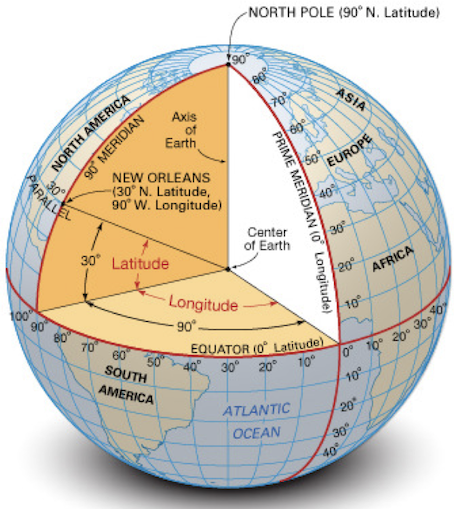
\includegraphics[width=4cm]{Longitude_latitude}
   \end{minipage} 
   \bigskip
   \begin{cadre}[B2][F4]
      \begin{center}
         Vidéo : \href{https://www.youtube.com/watch?v=lpYEuHeecko}{{\bf Les fondamentaux : latitude et longitude}, chaîne YouTube {\it La Classe d'Histoire}.}
      \end{center}
   \end{cadre}
\end{debat}


%%%%%%%%%%%%%%%%%%%%%%%%%%%%%%%%
%%%%%%%%%%%%%%%%%%%%%%%%%%%%%%%%
\activites

\begin{activite}[Couples d'angles]
   {\bf Objectif :} faire découvrir la notion d'angles-internes et d'angles correspondants.
   {\renewcommand{\baselinestretch}{1.15}\selectfont
   \begin{QCM}
   \partie[préparation]
      Découper les trois bandelettes en bas de page. Ces bandes représentent deux droites $(d_1)$ et $(d_2)$ et une troisième droite $(\Delta)$ qui leur est sécante aux points $A$ et $B$. Placer une attache parisienne au niveau du point $A$ commun entre $(d_1)$ et $(\Delta)$ et une autre au niveau du point $B$ commun entre $(d_2)$ et $(\Delta)$. \\
      Combien d'angles sont-ils matérialisés par cette configuration ?
   \partie[angles alternes-internes]
   \ \\ [-11mm]
      \begin{enumerate}
         \item Prendre deux jetons, les placer sur deux angles vérifiant les conditions suivantes :
            \begin{itemize}
               \item les deux angles n'ont pas le même sommet ;
               \item ils sont situés de part et d'autre de la droite $(\Delta)$ ;
               \item ils sont situés \og entre \fg{} les droites $(d_1)$ et $(d_2)$.
            \end{itemize}
         Quelle est la mesure en degrés de chacun de ces deux angles ?
         \item Combien y a-t-il de telles paires d'angles ?
         Les angles ainsi construits sont dit {\bf alternes-internes}.
         \item Placer les bandelettes de telle sorte que les droites $(d_1)$ et $(d_2)$ soient parallèles, repérer deux angles alternes-internes par deux jetons puis donner la mesure de chacun de ces deux angles.
         \item En observant les résultats de la classe, quelle conjecture peut-on faire ?
      \end{enumerate}
    \partie[angles correspondants]
    \ \\ [-11mm]
      \begin{enumerate}
         \item Prendre deux jetons, les placer sur deux angles vérifiant les conditions suivantes :
            \begin{itemize}
               \item les deux angles n'ont pas le même sommet ;
               \item ils sont situés du même côté que la droite $(\Delta)$ ;
               \item l'un est situé \og entre \fg{} les droites $(d_1)$ et $(d_2)$, l'autre à l'extérieur.
            \end{itemize}
         Quelle est la mesure en degrés de chacun de ces deux angles ?
         \item Combien y a-t-il de telles paires d'angles ? \\
            Les angles ainsi construits sont dit {\bf correspondants}.
         \item Placer les bandelettes de telle sorte que les droites $(d_1)$ et $(d_2)$ soient parallèles, repérer deux angles alternes-internes par deux jetons puis donner la mesure de chacun de ces deux angles.
         \item En observant les résultats de la classe, quelle conjecture peut-on faire ?
      \end{enumerate}
   \end{QCM}}
   \begin{pspicture}(0.5,1)(17.5,5)
      \psline(0.75,0.75)(17.25,0.75)
      \rput(1,1.1){$(d_1)$}
      \rput(12,1.25){$A$}
      \psline(0.75,2.25)(17.25,2.25)
      \rput(1,2.6){$(\Delta)$}
      \rput(6,2.75){$B$}
      \rput(12,2.75){$A$}
      \psline(0.75,3.75)(17.25,3.75)
      \rput(1,4.1){$(d_2)$}
      \rput(6,4.25){$B$}
      \psdots(12,0.75)(6,2.25)(12,2.25)(6,3.75)
      \psset{linecolor=gray}
      \psframe(0,0)(18,4.5)
      \psline(0,1.5)(18,1.5)
      \psline(0,3)(18,3)
   \end{pspicture}
\end{activite}


%%%%%%%%%%%%%%%%%%%%%%%%%%%%%%%%
%%%%%%%%%%%%%%%%%%%%%%%%%%%%%%%%
\cours 

%%%%%%%%%%%%%%%%%%%%%%%%%%%%%%%%%%%%%%%
\section{Mesure d'angles particuliers : rappels}

\begin{minipage}{10cm}
   \begin{pspicture}(-5,0.25)(5,2.5)
      \rput(0,-0.3){O}
      \rput(3.8,0){angle nul : \udeg{0}}
      \pswedge[fillstyle=solid,fillcolor=B2,linecolor=B2](0,0){1.5}{0}{90}
      \rput(2.5,1.5){\parbox{2.1cm}{\textcolor{B2}{angle aigu : \\ \udeg{0} < \pswedge[fillstyle=solid,fillcolor=B2,linecolor=B2](0.2,0){0.3}{0}{90} \qquad < \udeg{90}}}}
      \pswedge[fillstyle=solid,fillcolor=A1,linecolor=A1](0,0){1.5}{90}{180}
      \rput(-2.5,1.5){\parbox{2.5cm}{\textcolor{A1}{angle obtus : \\ \udeg{90} < \pswedge[fillstyle=solid,fillcolor=A1,linecolor=A1](0.4,0){0.3}{90}{180} \quad\; < \udeg{180}}}}
      \rput(0,2.5){angle droit : \udeg{90}}
      \rput(-3.8,0){angle plat : \udeg{180}}
      \psline(-2.5,0)(2.5,0)
      \psline(0,2)
   \end{pspicture}   
\end{minipage}
\begin{minipage}{5.5cm}
   Dans cette configuration, la somme des deux angles mesure \udeg{180}, on dit que ces angles sont supplémentaires. \\
   \begin{pspicture}(7,1.5)
      \psline(0.5,0)(5.5,0)
      \psline(3,0)(1.8,1.2)
      \psarc[linecolor=B1](3,0){0.7}{135}{180}
      \rput(2,0.4){\textcolor{B1}{\udeg{45}}}
      \psarc[linecolor=A1](3,0){0.5}{0}{135}
      \rput(3.6,0.7){\textcolor{A1}{\udeg{135}}}
   \end{pspicture}
\end{minipage}


%%%%%%%%%%%%%%%%%%%%%%%%%%%%%%%%
\section{Angles alternes-internes et correspondants}

\parbox{8cm}{Lorsque deux droites sont coupées par une droite sécante $(\Delta)$, on obtient huit angles. \\
{\it Dans la suite du cours, on se place dans cette configuration.}}
\hfill
\parbox{6.5cm}{\psset{unit=0.7}
   \begin{pspicture}(-0.5,-0.25)(6,3.5)
      \psline(0,1.5)(6,0.5)
      \psline(1,3)(6,3)
      \psline(1,0)(5,4)
      \psarc[linecolor=B2,doubleline=true](4,3){0.7}{0}{45}
      \rput(5,3.4){\textcolor{B2}{\small $A_2$}}
      \psarc[linecolor=J1,doubleline=true](4,3){0.7}{180}{225}
      \rput(3,2.5){\textcolor{J1}{\small $A_4$}}
      \psarc[linecolor=A1](4,3){0.5}{45}{180}
      \rput(3.7,3.8){\textcolor{A1}{\small $A_1$}}
      \psarc[linecolor=G1](4,3){0.5}{225}{0}
      \rput(4.35,2.25){\textcolor{G1}{\small $A_3$}}
      \psarc[linecolor=B2,doubleline=true](2.15,1.15){0.7}{-10}{45}
      \rput(3.2,1.4){\textcolor{B2}{\small $B_2$}}
      \psarc[linecolor=J1,doubleline=true](2.15,1.15){0.7}{170}{225}
      \rput(1.1,0.7){\textcolor{J1}{\small $B_4$}}
      \psarc[linecolor=A1](2.15,1.15){0.5}{45}{170}
      \rput(1.8,1.9){\textcolor{A1}{\small $B_1$}}
      \psarc[linecolor=G1](2.15,1.15){0.5}{225}{-10}
      \rput(2.4,0.3){\textcolor{G1}{\small $B_3$}}
      \rput(0.7,-0.3){$(\Delta)$}
      \rput(-0.5,1.5){$(d_1)$}
      \rput(0.5,3){$(d_2)$}
   \end{pspicture}}

\begin{definition}
   Deux angles sont {\bf alternes-internes} s'ils n'ont pas le même sommet, qu'ils sont situés de part et d'autre de la sécante $(\Delta)$ et qu'ils se situent \og entre \fg{} les droites $(d_1)$ et $(d_2)$.
\end{definition}

\begin{exemple*1}
Sur la figure, il y a deux couples d'angles alternes-internes : $A_4$ et $B_2$ ; $A_3$ et $B_1$.
\end{exemple*1}

\bigskip

\begin{definition}
   Deux angles sont {\bf correspondants} s'ils n'ont pas le même sommet, qu'ils sont situés du même côté de la sécante $(\Delta)$, l'un entre les deux droites $(d_1)$ et $(d_2)$ et l'autre à l'extérieur.
\end{definition}

\begin{exemple*1}
Sur la figure, il existe quatre couples d'angles correspondants :  $A_1$ et $B_1$ ; $A_2$ et $B_2$ ; $A_3$ et $B_3$ ; $A_4$ et $B_4$.
\end{exemple*1}


%%%%%%%%%%%%%%%%%%%%%%%%%%%%%%%%
\section{Et si les droites sont parallèles ?}

\begin{propriete}
   \begin{itemize}
      \item Si les deux droites $(d_1)$ et $(d_2)$ sont parallèles, alors les angles alternes-internes et les angles correspondants sont égaux deux à deux.
      \item Si deux angles alternes-internes ou deux angles correspondants sont égaux, alors les droites $(d_1)$ et $(d_2)$ sont parallèles.
   \end{itemize}
   \ \\ [-14mm]
\end{propriete}

\begin{exemple}
   {\psset{unit=0.9}
   \begin{pspicture}(0,0.3)(6,3.2)
      \psline(1,1)(6,1)
      \psline(1,2.5)(6,2.5)
      \psline(2,0)(4,3)
      \rput(2.4,2.1){$\alpha =\udeg{56}$}
      \rput(3.5,1.5){$\beta$}
      \rput(1.8,0.5){$\gamma$}
      \psarc[linecolor=B2,doubleline=true](3.67,2.5){0.6}{182}{234}
      \psarc[linecolor=A1,doubleline=true](2.67,1){0.6}{2}{55}
      \psarc[linecolor=J1,doubleline=true](2.67,1){0.6}{182}{233}
      \rput(5.5,1.75){\parbox{1.5cm}{\small droites\\parallèles}}
   \end{pspicture}}
   \correction
   Mesures de $\beta$ et $\gamma$, sachant que les droites sont parallèles :
   \begin{itemize}
      \item $\alpha$ et $\beta$ sont des angles alternes-internes, ils ont donc même mesure. D'où : $\beta =\alpha =\udeg{56}$.
      \item $\alpha$ et $\gamma$ sont des angles correspondants, ils ont donc même mesure. D'où : $\gamma =\alpha =\udeg{56}$.
   \end{itemize}
\end{exemple}


%%%%%%%%%%%%%%%%%%%%%%%%%%%%%%%%
%%%%%%%%%%%%%%%%%%%%%%%%%%%%%%%%
\exercicesbase

\begin{colonne*exercice}

\begin{exercice} %1
   Au regard de la figure, que peut-on dire des angles :
   \begin{colenumerate}{3}
      \item 1 et 5 ?
      \item 2 et 6 ?
      \item 4 et 6 ?
      \item 3 et 7 ?
      \item 3 et 5 ?
      \item 4 et 8 ?
   \end{colenumerate}
   {\psset{unit=0.9}
   \begin{pspicture}(-0.5,0)(6,4.2)
      \psline(0,1.5)(6,0.5)
      \psline(1,3)(6,3)
      \psline(1,0)(5,4)
      \psarc(4,3){0.7}{0}{45}
      \rput(5,3.4){2}
      \psarc(4,3){0.7}{180}{225}
      \rput(3,2.5){4}
      \psarc(4,3){0.5}{45}{180}
      \rput(3.7,3.8){1}
      \psarc(4,3){0.5}{225}{0}
      \rput(4.35,2.25){3}
      \psarc(2.15,1.15){0.7}{-10}{45}
      \rput(3.2,1.4){6}
      \psarc(2.15,1.15){0.7}{170}{225}
      \rput(1.1,0.7){8}
      \psarc(2.15,1.15){0.5}{45}{170}
      \rput(1.8,1.9){5}
      \psarc(2.15,1.15){0.5}{225}{-10}
      \rput(2.4,0.3){7}
   \end{pspicture}}
\end{exercice}

\begin{corrige}
   \ \\ [-5mm]
   \begin{enumerate}
      \item Les angles 1 et 5 sont {\blue correspondants}.
      \item Les angles 2 et 6 sont {\blue correspondants}.
      \item Les angles 4 et 6 sont {\blue alternes-internes}.
      \item Les angles 3 et 7 sont {\blue correspondants}.
      \item Les angles 3 et 5 sont {\blue alternes-internes}.
      \item Les angles 4 et 8 sont {\blue correspondants}.
   \end{enumerate}
\end{corrige}

\medskip


\begin{exercice} %2
   Dans la configuration suivante, citer :
   \begin{enumerate}
       \item la sécante ;
       \item deux angles correspondants ;
       \item deux angles alternes-internes.
   \end{enumerate}
   \begin{pspicture}(-3,-1.5)(3,1.2)
      \psline(-1.5,0)(2,0)
      \psline(-1,0.75)(2,-1.5)
      \psline(-1.5,-1)(2.5,-1)
      \rput(-1.75,0){$x$}
      \rput(-1.2,0.9){$y$}
      \rput(2.25,0){$t$}
      \rput(2.25,-1.6){$s$}
      \rput(2.75,-1){$u$}
      \rput(0.2,0.25){$O$}
      \rput(1.5,-0.75){$I$}
      \rput(-1.75,-1){$k$}
   \end{pspicture}
\end{exercice}

\begin{corrige}
   \ \\ [-5mm]
   \begin{enumerate}
       \item La sécante est {\blue la droite $(ys)$}.
       \item Il y a quatre couples d'angles correspondants : \\
          {\blue $\widehat{yOt}$ et $\widehat{OIu}$ ; \\
          $\widehat{yOx}$ et $\widehat{OIk}$ ; \\
          $\widehat{tOI}$ et $\widehat{uIs}$ ; \\
          $\widehat{xOI}$ et $\widehat{kIs}$}.
       \item Il y a deux couples d'angles alternes-internes : \\
          {\blue $\widehat{xOI}$ et $\widehat{OIu}$ \\
          $\widehat{tOI}$ et $\widehat{OIk}$}.
   \end{enumerate}
\end{corrige}

\medskip


\begin{exercice} %3
   Sur cette figure, les droites $(xy)$ et $(zt)$, ainsi que les droites $(su)$ et $(fg)$, sont parallèles. \\
   Compléter le tableau suivant lorsque c'est possible.
   \begin{center}
   \psset{xunit=2cm}
      \begin{pspicture}(-1.5,-2.2)(2.5,1.2)
         \psline(-1,0)(2,0)
         \psline(-1,-1)(2,-1)
         \psline(-1,1)(1,-2)
         \psline(0,1)(2,-2)
         \psline(0,-2)(1,1)
         \rput(-1.1,0){$x$}
         \rput(2.1,0){$y$}
         \rput(-1.1,-1){$z$}
         \rput(2.1,-1){$t$}
         \rput(-1.1,1.1){$s$}
         \rput(1.1,-2.1){$u$}
         \rput(-0.1,1.1){$f$}
         \rput(2.1,-2.1){$g$}      
         \rput(-0.1,-2.1){$h$}
         \rput(1.1,1.1){$i$}
         \rput(-0.3,0.25){$A$}
         \rput(0.85,0.2){$B$}
         \rput(0.3,-0.65){$C$}
         \rput(1.4,-0.65){$D$}
      \end{pspicture}
   \end{center}
   \begin{tabular}{|C{2.2}|*{4}{C{0.9}|}}
      \hline
      angle & $\widehat{yBg}$ & $\widehat{zCi}$ & $\widehat{fBi}$ & $\widehat{uCi}$ \\
      \hline
       alterne-interne & & & & \\
       \hline
       correspondant & & & & \\
       \hline
   \end{tabular}
\end{exercice}

\begin{corrige}
   On obtient le tableau suivant, par exemple : \\ \smallskip
   {\hautab{1.5}
   \begin{tabular}{|C{1.8}|*{4}{C{0.85}|}}
      \hline
      angle & $\widehat{yBg}$ & $\widehat{zCi}$ & $\widehat{fBi}$ & $\widehat{uCi}$ \\
      \hline
       \footnotesize Angles alterne-interne & \textcolor{blue}{$\widehat{zDf}$ $\widehat{BDC}$\dots} & \textcolor{blue}{$\widehat{hBy}$ $\widehat{yBC}$\dots} & \textcolor{blue}{$\varnothing$} & \textcolor{blue}{$\widehat{fBh}$ $\widehat{CBf}$\dots} \\
       \hline
       \footnotesize Angles correspondant & \textcolor{blue}{$\widehat{tDg}$ $\widehat{yAu}$\dots} & \textcolor{blue}{$\widehat{xBi}$ $\widehat{iBA}$\dots} & \textcolor{blue}{$\widehat{sCi}$ $\widehat{BCA}$\dots} & \textcolor{blue}{$\widehat{gBi}$ $\widehat{iBD}$\dots} \\
       \hline
   \end{tabular}} \medskip
\end{corrige}

\medskip


\begin{exercice} %4
   Anita pense que l'une des deux paires de droites $(d_1)$ et $(d_2)$ est parallèle. A-t-elle raison ? \\
   \begin{pspicture}(0,0.5)(4,2.7)
      \pstGeonode[PointSymbol=none,PointName=none](0,2.5){A}(4,0){B}(0,1){C}(3,2){D}(1,0){E}(4,1){F}
      \pstInterLL[PointName=none,PointSymbol=none]{A}{B}{C}{D}{H}
       \pstInterLL[PointName=none,PointSymbol=none]{A}{B}{E}{F}{I}
      \pstLineAB{A}{B}
      \pstLineAB{C}{D}
      \pstLineAB{E}{F}
      \pstMarkAngle{D}{H}{A}{\udeg{119}}
      \pstMarkAngle{B}{I}{F}{\udeg{61}}
      \rput(0.5,0.8){$(d_1)$}
      \rput(1.7,-0.2){$(d_2)$}
   \end{pspicture}   
   \begin{pspicture}(-0.8,0.6)(3.5,3.3)
      \pstGeonode[PointSymbol=none,PointName=none](0,1.5){A}(3,1){B}(0,0){C}(1.5,3){D}(1.5,0){E}(2.5,2.5){F}
      \pstInterLL[PointName=none,PointSymbol=none]{A}{B}{C}{D}{H}
       \pstInterLL[PointName=none,PointSymbol=none]{A}{B}{E}{F}{I}
      \pstLineAB{A}{B}
      \pstLineAB{C}{D}
      \pstLineAB{E}{F}
      \pstMarkAngle{B}{H}{D}{\udeg{59}}
      \pstMarkAngle{E}{I}{B}{\udeg{111}}
      \rput(1,2.8){$(d_1)$}
      \rput(3,2.5){$(d_2)$}
   \end{pspicture}
\end{exercice}

\begin{corrige}
   Oui, Anita a raison : \\
   \begin{itemize}
      \item Première figure : l'angle supplémentaire à \udeg{119} de l'autre côté de $(d_1)$ vaut $\udeg{180}-\udeg{119} =\udeg{61}$. \\
      On a deux angles correspondants de même mesure donc, {\blue les droites $(d_1)$ et $(d_2)$ sont parallèles}.
      \item Deuxième figure : l'angle supplémentaire à \udeg{111} de l'autre côté de $(d_2)$ vaut $\udeg{180}-\udeg{111} =\udeg{69}$. \\
      On a deux angles alternes-internes de mesures différentes donc, {\blue $(d_1)$ et $(d_2)$ ne sont pas parallèles}.
   \end{itemize}
\end{corrige}

\bigskip


\begin{exercice} %5
   Dans la figure ci-dessous, on sait que les droites $(xy)$ et
$(tz)$ sont parallèles et on connaît la mesure de deux angles. En utilisant les données de la figure :
   \begin{enumerate}
       \item Donner la mesure en degrés des angles suivants : $\widehat{IJK}$, puis $\widehat{JKI}$, puis $\widehat{rIy}$, puis $\widehat{yIJ}$, puis $\widehat{xIK}$ et enfin $\widehat{KIJ}$.
       \item En déduire la nature du triangle $IJK$?
   \end{enumerate}
   \begin{pspicture}(-2.5,-0.5)(4.8,3.2)
        \pstGeonode[PointSymbol=none,PosAngle={180,120,-120,0,180,0}](-1,0){z}(0,0){K}(2,0){J}(4,0){t}
        \pstRotation[PointSymbol=none,PosAngle=150,RotAngle=60]{K}{J}[I]
        \pstOIJGeonode[PointSymbol=none,PosAngle={180,0,60,120}](-1,1){x}{K}{J}{I}(1.5,1){y}(0,1.4){s}(-.4,1.4){r}
        \pstLineAB{x}{y}
        \pstLineAB{z}{t}
        \pstLineAB[nodesepA=-.9,nodesepB=-.5]{I}{K}
        \pstLineAB[nodesepA=-.9, nodesepB=-.5]{I}{J}
        \pstMarkAngle{t}{J}{r}{120°}
        \pstMarkAngle{y}{I}{s}{60°}
    \end{pspicture}
\end{exercice}

\begin{corrige}
\ \\ [-5mm]
   \begin{enumerate}
       \item $\bullet$ Les angles $\widehat{IJK}$ et $\widehat{IJt}$ sont supplémentaires donc, ${\blue \widehat{IJK}} =180\up{\circ}-120\up{\circ}° ={\blue 60\up{\circ}}$. \\
          $\bullet$ Les angles $\widehat{JKI}$ et $\widehat{yIS}$ sont correspondants et $\widehat{yIS} =60\up{\circ}$ donc, {\blue $\widehat{JKI} =60\up{\circ}$}. \\
          $\bullet$ Les angles $\widehat{rIy}$ et $\widehat{IJt}$ sont correspondants et $\widehat{IJt} =120\up{\circ}$ donc, {\blue $\widehat{rIy} =120\up{\circ}$}. \\
          $\bullet$ Les angles $\widehat{yIJ}$ et $\widehat{rIy}$ sont supplémentaires donc, ${\blue \widehat{yIJ}} =180\up{\circ}-120\up{\circ}° ={\blue 60\up{\circ}}$. \\
          $\bullet$ Les angles $\widehat{xIK}$ et $\widehat{sIy}$ sont opposés par le sommet donc, ${\blue \widehat{xIK}} =\widehat{sIy} ={\blue 60\up{\circ}}$. Et enfin : \\
          ${\blue \widehat{KIJ}} =180\up{\circ} -\widehat{xIK}-\widehat{yIJ} =180\up{\circ}-60\up{\circ}-60\up{\circ} ={\blue 60\up{\circ}}$.
       \item Les trois angles du triangle sont égaux, donc {\blue le triangle $IJK$ est équilatéral}.
   \end{enumerate}
\end{corrige}

\medskip


\begin{exercice} %6
   Sur la figure ci-dessous :
   \begin{itemize}
      \item les droites $(ab), (cd)$ et $(ef)$ sont parallèles ;
      \item $R$ est un point de $(ab)$, $S$ un point de $(cd)$ et $T$ un point de $(ef)$ tels que $\widehat{bRS} =\udeg{20}$ et $\widehat{RST} =\udeg{57}$.
   \end{itemize}
   Calculer la mesure de l'angle $\widehat{STf}$. \\
   \begin{pspicture}(-1,0)(7,3.8)
      \pstGeonode[PointSymbol=none,PosAngle={90}](0,0.5){e}(2,0.5){T}(7,0.5){f}(0,2){c}(4,2){S}(7,2){d}(0,3){a}(2,3){R}(7,3){b}
      \pstLineAB{a}{b}
      \pstLineAB{c}{d}
      \pstLineAB{e}{f}
      \pstLineAB{R}{S}
      \pstLineAB{S}{T}
      \pstMarkAngle{S}{R}{b}{}
      \rput(3,2.8){\udeg{20}}
      \pstMarkAngle[MarkAngleType=double]{R}{S}{T}{}
      \rput(3.2,1.8){\udeg{57}}
      \pstMarkAngle{f}{T}{S}{?}
   \end{pspicture}
\end{exercice}

\begin{corrige}
   \begin{itemize}
      \item Les angles $\widehat{bRS}$ et $\widehat{RSc}$ sont alternes-internes et les droites $(ab)$ et $(cd)$ sont parallèles donc : $\widehat{RSc} =\widehat{bRS} =\udeg{20}$.
      \item On décompose l'angle $\widehat{RST}$ : $\widehat{RST} =\widehat{RSc}+\widehat{cST}$ donc, $\widehat{cST} =\widehat{RST} -\widehat{RSc} =\udeg{57}-\udeg{20} =\udeg{37}$.
      \item Les angles $\widehat{cST}$ et $\widehat{STf}$ sont alternes-internes et les droites $(cd)$ et $(ef)$ sont parallèles donc : $\widehat{STf} =\widehat{cST} =\blue \udeg{37}$.
   \end{itemize}
\end{corrige}

\medskip


\begin{exercice} %7
   Nora possède un champ en forme de quadrilatère $NORA$ dont les côtés $(NO)$ et $(RA)$ sont parallèles. Elle prend la mesure de deux angles et se demande si son quadrilatère peut être un parallélogramme.
   \begin{enumerate}
      \item Écrire sur le schéma ci-dessous la mesure de tous les angles existants.
      \item Les droites $(NA)$ et $(OR)$ sont-elles parallèles ?
      \item Quelle est alors la nature du quadrilatère $NORA$ ?
   \end{enumerate}
   \psset{unit=0.7}
   \begin{pspicture}(-1,0)(10,6)
      \pstGeonode[PointSymbol=none,PointName=none](0,1){a}(10,1){b}(0,4){c}(10,4){d}(0.33,0){f}(4,5.5){g}(6.33,0){h}(9,5){j}
      \pstLineAB{a}{b}
      \pstLineAB{c}{d}
      \pstLineAB{f}{g}
      \pstLineAB{h}{j}
      \pstInterLL[PosAngle=-45,PointSymbol=none]{a}{b}{f}{g}{A}
      \pstInterLL[PosAngle=-45,PointSymbol=none]{a}{b}{h}{j}{R}
      \pstInterLL[PosAngle=-45,PointSymbol=none]{c}{d}{f}{g}{N}
      \pstInterLL[PosAngle=-45,PointSymbol=none]{c}{d}{h}{j}{O}
      \pstMarkAngle{j}{O}{N}{\udeg{121}}
      \pstMarkAngle{R}{A}{N}{\udeg{49}}
   \end{pspicture}
\end{exercice}

\begin{corrige}
\ \\ [-5mm]
   \begin{enumerate}
      \item Schéma du terrain de Nora : \\
      {\psset{unit=0.7}
   \begin{pspicture}(0,-0.5)(10,6)
      \pstGeonode[PointSymbol=none,PointName=none](0,1){a}(10,1){b}(0,4){c}(10,4){d}(0.33,0){f}(4.5,5.5){g}(6.33,0){h}(9,5){j}
      \pstLineAB{a}{b}
      \pstLineAB{c}{d}
      \pstLineAB{f}{g}
      \pstLineAB{h}{j}
      \pstInterLL[PosAngle=-45,PointSymbol=none,PointName=none]{a}{b}{f}{g}{S}
      \pstInterLL[PosAngle=-45,PointSymbol=none,PointName=none]{a}{b}{h}{j}{E}
      \pstInterLL[PosAngle=-45,PointSymbol=none,PointName=none]{c}{d}{f}{g}{I}
      \pstInterLL[PosAngle=-45,PointSymbol=none,PointName=none]{c}{d}{h}{j}{N}
      \pstMarkAngle{j}{N}{I}{\udeg{121}}
      \pstMarkAngle{E}{S}{I}{\udeg{49}}
      \pstMarkAngle{I}{N}{E}{\blue\udeg{59}}
      \pstMarkAngle{E}{N}{d}{\blue\udeg{121}}
      \pstMarkAngle{d}{N}{j}{\blue\udeg{59}}
      \pstMarkAngle{b}{E}{N}{\blue\udeg{59}}
      \pstMarkAngle{h}{E}{b}{\blue\udeg{121}}
      \pstMarkAngle{N}{E}{S}{\blue\udeg{121}}
      \pstMarkAngle{S}{E}{h}{\blue\udeg{59}}
      \pstMarkAngle{f}{S}{E}{\blue\udeg{131}}
      \pstMarkAngle{I}{S}{a}{\blue\udeg{131}}
      \pstMarkAngle{a}{S}{f}{\blue\udeg{49}}
      \pstMarkAngle{f}{S}{E}{\blue\udeg{131}}
      \pstMarkAngle{I}{S}{a}{\blue\udeg{131}}
      \pstMarkAngle{g}{I}{e}{\blue\udeg{131}}
      \pstMarkAngle{e}{I}{f}{\blue\udeg{49}}
      \pstMarkAngle{d}{I}{g}{\blue\udeg{49}}
      \pstMarkAngle{f}{I}{d}{\blue\udeg{131}}
   \end{pspicture}}
      \item Si les droites $(NA)$ ET $(OR)$ étaient parallèles, les angles correspondants en $N$ et $O$ par exemple seraient égaux, ce qui n'est pas le cas ici (\udeg{131}$\neq$\udeg{121}) donc, {\blue ces droites ne sont pas parallèles}.
      \item Dans le quadrilatère $NORA$, les droites $(NO)$ et $(RA)$ sont parallèles, mais les droites $(NA)$ et $(OR)$ ne le sont pas donc, {\blue le quadrilatère $NORA$ est un trapèze}.   
   \end{enumerate}
\end{corrige}

\end{colonne*exercice}


%%%%%%%%%%%%%%%%%%%%%%%%%%%%%%%%
%%%%%%%%%%%%%%%%%%%%%%%%%%%%%%%%
\Recreation

\begin{enigme}[Le flexagone]
   {\it Arthur Stone}, étudiant britannique de 23 ans, aurait découvert de curieuses formes géométriques polygonales en 1939, en découpant les feuilles de papier au format américain pour les transformer au format européen, plus étroit. Il lui restait alors des bandes qu'il se mit à plier pour obtenir des formes géométriques dont certaines se révélèrent \og flexibles \fg. Le premier {\bf flexagone} qu'il découvrit aurait été construit grâce à neuf triangles équilatéraux pliés puis assemblés pour former un hexagone. \medskip

   \partie[construction du flexagone] \vspace*{-5mm}
      \begin{enumerate}
         \item Reproduire, puis découper la figure ci-dessous, composée de 9 triangles équilatéraux de côté 5 cm. \\
            {\psset{unit=0.5}
               \begin{pspicture}(-8,-0.2)(10,2.2)
                  \multido{\n=0+2}{5}{\rput(\n,0){\pspolygon(0,0)(2,0)(2;60)}}
                  \psline(2;60)(9,1.732)
               \end{pspicture}}
         \item Marquer le pli vallée au niveau de l'arête commune entre le 3\up{e} et le 4\up{e} triangle, puis replier vers le haut les trois premiers triangles. \\
            {\psset{unit=0.5}
               \begin{pspicture}(-8,-0.2)(10,3.6)
                  \multido{\n=4+2}{3}{\rput(\n,0){\pspolygon(0,0)(2,0)(2;60)}}
                  \pspolygon[fillstyle=solid,fillcolor=lightgray](4,0)(3,1.732)(4,3.464)(6,3.464)(6,3.464)
                  \psline(3,1.732)(9,1.732)
                  \psline(4,3.464)(5,1.732)
               \end{pspicture}}
         \item Marquer le pli montagne au niveau de l'arête commune entre le 6\up{e} et le 7\up{e} triangle, puis replier vers le haut les trois derniers triangles en faisant passer le dernier triangle sur le premier triangle. \\
            Enfin, mettre un morceau de ruban adhésif pour maintenir le premier et le dernier triangle ensemble. \\
            {\psset{unit=0.5}
               \begin{pspicture}(-8,0)(13,5)
                  \rput(4,0){\pspolygon(0,0)(2,0)(2;60)}
                  \pspolygon[fillstyle=solid,fillcolor=lightgray](4,0)(3,1.732)(4,3.464)(6,3.464)(6,3.464)
                  \psline(3,1.732)(7,1.732)
                  \psline(4,3.464)(5,1.732)
                  \psline(6,0)(7,1.732)
                  \pspolygon[fillstyle=solid,fillcolor=gray](5,1.732)(7,1.732)(6,3.464)
                  \psline{->}(8,3)(12,3)
                  \rput(10,3.5){\it\small passer le dernier}
                  \rput(10,2.5){\it\small triangle au dessus}
               \end{pspicture}
               \begin{pspicture}(3,0)(7,5)
                  \rput(4,0){\pspolygon(0,0)(2,0)(2;60)}
                  \pspolygon[fillstyle=solid,fillcolor=lightgray](4,0)(3,1.732)(4,3.464)(6,3.464)
                  \pspolygon[fillstyle=solid,fillcolor=gray](5,1.732)(7,1.732)(6,3.464)(4,3.464)
                  \psline(3,1.732)(7,1.732)(6,0)
                  \psline(5,1.732)(6,3.464)   
                  \rput(5,4.5){\it scotch} 
                  \psline{->}(5,4.2)(5,3.7)    
               \end{pspicture}}
      \end{enumerate}
               
   \partie[utilisation du flexagone] \vspace*{-5mm}
      \begin{enumerate}
         \item On obtient un hexagone, ou plus précisément un hexaflexagone. Dessiner ou colorier les deux faces obtenues.
         \item Marquer tous les plis dans les deux sens.
         \item Plier une arête sur deux en alternant les plis vallée et montagne de telle sorte que les soufflets soient en plis montagne, puis ouvrir : on obtient, de manière magique, une troisième face que l'on peut à son tour colorier. \medskip
            \begin{center}
               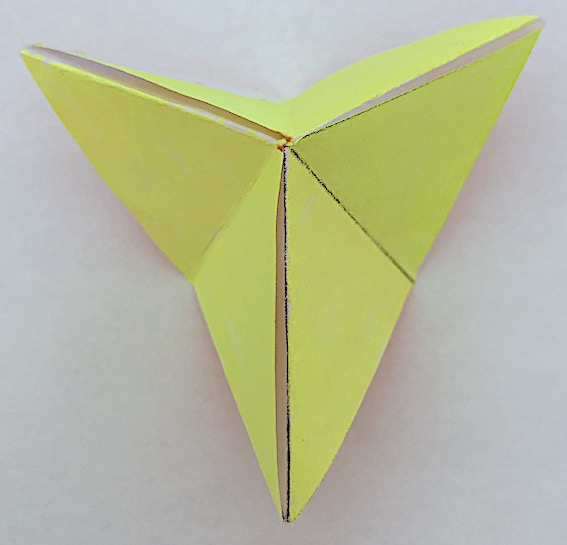
\includegraphics[width=3cm]{flexagone1} 
               \qquad
               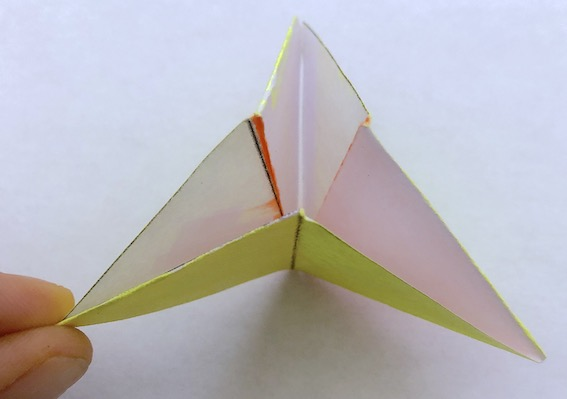
\includegraphics[width=4cm]{flexagone2} 
            \end{center}
         \item En réitérant le pliage, on obtient successivement les trois faces, une à une.
      \end{enumerate}

  {\bf Pour aller plus loin :}
  \begin{itemize}
      \item Un article, paru dan le magasine \og Pour la science \fg{} et écrit par Jean-Paul Delahaye, explique que l'on peut faire des flexagones avec autant de faces que l'on souhaite : \href{https://www.cristal.univ-lille.fr/~jdelahay/pls/2005/131.pdf}{\blue Le flexagone}
      \item Il existe également des sites spécialisés, comme \href{http://www.flexagon.net}{\blue Flexagone.net} qui propose de multiples modèles décorés à imprimer 
   \end{itemize}
\end{enigme}


\themaA
\graphicspath{{../../S03_En_route_vers_la_programmation/Images/}}

% Grille
\newcommand{\cn}{\psframe[fillstyle=solid,fillcolor=black](0,0)(1,1)}
\newcommand{\ho}{
\includegraphics[width=0.3cm]{Hercule}}
\newcommand{\po}{
\includegraphics[width=0.3cm]{pommier}}

% Commandes
\newcommand{\dep}{\pspolygon[fillstyle=solid,fillcolor=orange](6,1)(0,1)(0,0)(1,0)(1.25,-0.25)(1.5,0)(6.5,0)(6.5,0.5) \pswedge[fillstyle=solid,fillcolor=orange,linecolor=orange](6,0.5){0.5}{0}{90} \psarc(6,0.5){0.5}{0}{90} \put(0.5,0.3){\footnotesize Démarre}}
\newcommand{\av}[1]{\pspolygon[fillstyle=solid,fillcolor=green](0,0)(1,0)(1.25,-0.25)(1.5,0)(6.5,0)(6.5,1)(1.5,1)(1.25,0.75)(1,1)(0,1) \put(0.5,0.3){\footnotesize Avance de #1}}
\newcommand{\tg}{\pspolygon[fillstyle=solid,fillcolor=yellow](0,0)(1,0)(1.25,-0.25)(1.5,0)(6.5,0)(6.5,1)(1.5,1)(1.25,0.75)(1,1)(0,1) \put(0.5,0.3){\footnotesize Tourne à gauche}}
\newcommand{\td}{\pspolygon[fillstyle=solid,fillcolor=pink](0,0)(1,0)(1.25,-0.25)(1.5,0)(6.5,0)(6.5,1)(1.5,1)(1.25,0.75)(1,1)(0,1) \put(0.5,0.3){\footnotesize Tourne à droite}}
\newcommand{\fin}{\pspolygon[fillstyle=solid,fillcolor=orange](0,0)(6,0)(6.5,0.5)(6.5,1)(1.5,1)(1.25,0.75)(1,1)(0,1)(0,0) \pswedge[fillstyle=solid,fillcolor=orange,linecolor=orange](6,0.5){0.5}{-90}{0} \psarc(6,0.5){0.5}{-90}{0} \put(0.5,0.3){\footnotesize Prends les pommes}}

% Fourmi
\newcommand{\fourmi}[3]{\rput{#3}(#1,#2){\psdot[linecolor=red,dotstyle=triangle*,linewidth=1mm](0,0)}}
\newcommand{\cub}{\psframe[fillstyle=solid,fillcolor=black](0,0)(1,1)}

\chapter{En route vers la\\programmation}
\label{S03}


%%%%%%%%%%%%%%%%%%%%%%%%%%%%%%%%
%%%%%%%%%%%%%%%%%%%%%%%%%%%%%%%%
\begin{autoeval}
   \small
   Niveau 1 (possibilité d'aller au delà).
   \begin{enumerate}
      \item Il réalise des activités d’algorithmique débranchée.
      \item Il met en ordre et/ou complète des blocs fournis par le professeur pour construire un programme simple sur un logiciel de programmation.
      \item Il écrit un script de déplacement ou de construction géométrique utilisant des instructions conditionnelles et/ou la boucle \og Répéter \dots{} fois \fg.
   \end{enumerate}
\end{autoeval}

\begin{prerequis}
   \begin{itemize}
      \item Notions d'algorithme et de programme. 
      \item Notion de variable informatique.
      \item Déclenchement d'une action par un événement.
      \item Séquences d'instructions, boucles, instructions conditionnelles.
      \item[\com] Écrire, mettre au point (tester, corriger) et exécuter un programme en réponse à un problème donné.
   \end{itemize}
\end{prerequis}

\vfill

\begin{debat}[Débat : la fourmi de Langton : que se passe-t-il ensuite ?] 
   La {\bf fourmi de Langton}, du nom de son inventeur scientifique américain {\it Christopher Langton}, est un petit programme informatique inventé vers la fin des années 1980. Il consiste en un automate qui se déplace dans un quadrillage suivant des règles simples. Il modélise le fait qu'un ensemble de comportements élémentaires peut donner lieu à un comportement complexe.
   \begin{center}
      {\psset{unit=0.2}
      \begin{pspicture}(0,0)(13,13)
         \fourmi{6.5}{6.5}{-90}
         \rput(2,0){\cub} \rput(3,0){\cub}
         \rput(1,1){\cub} \rput(2,1){\cub} \rput(9,1){\cub} \rput(10,1){\cub}
         \rput(0,2){\cub} \rput(2,2){\cub} \rput(3,2){\cub} \rput(5,2){\cub} \rput(8,2){\cub} \rput(11,2){\cub}
         \rput(0,3){\cub} \rput(3,3){\cub} \rput(5,3){\cub} \rput(6,3){\cub} \rput(7,3){\cub} \rput(9,3){\cub} \rput(10,3){\cub} \rput(11,3){\cub}
         \rput(1,4){\cub} \rput(3,4){\cub} \rput(10,4){\cub} \rput(12,4){\cub}
         \rput(3,5){\cub} \rput(4,5){\cub} \rput(8,5){\cub} \rput(9,5){\cub}
         \rput(3,6){\cub} \rput(4,6){\cub} \rput(5,6){\cub} \rput(7,6){\cub} \rput(8,6){\cub} \rput(9,6){\cub}
         \rput(3,7){\cub} \rput(4,7){\cub} \rput(8,7){\cub} \rput(9,7){\cub}
         \rput(0,8){\cub} \rput(2,8){\cub} \rput(9,8){\cub} \rput(11,8){\cub}
         \rput(0,9){\cub} \rput(1,9){\cub} \rput(2,9){\cub} \rput(5,9){\cub} \rput(6,9){\cub} \rput(7,9){\cub} \rput(9,9){\cub} \rput(12,9){\cub}
         \rput(1,10){\cub} \rput(4,10){\cub} \rput(7,10){\cub} \rput(9,10){\cub} \rput(10,10){\cub} \rput(12,10){\cub}
         \rput(2,11){\cub} \rput(3,11){\cub} \rput(10,11){\cub} \rput(11,11){\cub}
         \rput(9,12){\cub} \rput(10,12){\cub}
      \end{pspicture}}
   \end{center}
   \bigskip
   \begin{cadre}[B2][J4]
      \begin{center}
         Vidéo : \href{https://www.youtube.com/watch?v=qZRYGxF6D3w}{\bf La fourmi de Langton}, chaîne YouTube {\it Science étonnante}.
      \end{center}
   \end{cadre}
\end{debat}


%%%%%%%%%%%%%%%%%%%%%%%%%%%%%%%%%%%
%%%%%%%%%%%%%%%%%%%%%%%%%%%%%%%%%%%
\activites

\begin{activite}[La fourmi de Langton]
   {\bf Objectifs :} suivre un algorithme de déplacement ; se repérer dans le plan dans un repérage relatif.
   \begin{QCM}
      La fourmi de Langton est un automate qui se déplace dans un quadrillage suivant les règles suivantes :
      \begin{itemize}
         \item au départ, toutes les cases sont de la même couleur, ici blanches ;
         \item si la fourmi est sur une case blanche, elle tourne de \udeg{90} vers la droite, change la couleur de la case en noir et avance d'une case ;
         \item si la fourmi est sur une case noire, elle tourne de \udeg{90} vers la gauche, change la couleur de la case en blanc et avance d'une case.
      \end{itemize}
      Compléter dans les quadrillages ci-dessous les quinze premières étapes du déplacement de la fourni.
      \begin{center}
      \psset{unit=0.5,subgriddiv=1,gridlabels=0mm,gridcolor=gray}
      \small
      \begin{pspicture}(0,-0.7)(7,7)
         \psgrid(0,0)(7,7)
         \fourmi{3.5}{3.5}{0}
          \rput(3.5,-0.5){étape 0}
      \end{pspicture}
      \quad
      \begin{pspicture}(0,-0.7)(7,7)
         \psframe[fillstyle=solid,fillcolor=darkgray](3,3)(4,4)
         \psgrid(0,0)(7,7)
         \fourmi{4.5}{3.5}{-90}
         \rput(3.5,-0.5){étape 1}
      \end{pspicture}
      \quad
      \begin{pspicture}(0,-0.7)(7,7)  
         \psframe[fillstyle=solid,fillcolor=darkgray](3,3)(5,4)
         \psgrid(0,0)(7,7)
         \fourmi{4.5}{2.5}{180}
         \rput(3.5,-0.5){étape 2}
      \end{pspicture}
      \quad
      \begin{pspicture}(0,-0.7)(7,7)
         \psgrid(0,0)(7,7)
         \rput(3.5,-0.5){étape 3}
      \end{pspicture}
      \bigskip
      \begin{pspicture}(0,-0.7)(7,7)
         \psframe[fillstyle=solid,fillcolor=darkgray](3,2)(5,4)
         \psgrid(0,0)(7,7)
         \fourmi{3.5}{3.5}{0}
         \rput(3.5,-0.5){étape 4}
      \end{pspicture}
      \quad
      \begin{pspicture}(0,-0.7)(7,7)
         \psgrid(0,0)(7,7)
         \rput(3.5,-0.5){étape 5}
      \end{pspicture}
      \quad
      \begin{pspicture}(0,-0.7)(7,7)
         \psgrid(0,0)(7,7)
         \rput(3.5,-0.5){étape 6}
      \end{pspicture}
      \quad
      \begin{pspicture}(0,-0.7)(7,7)
         \psframe[fillstyle=solid,fillcolor=darkgray](2,3)(3,5)
         \pspolygon[fillstyle=solid,fillcolor=darkgray](3,2)(5,2)(5,4)(4,4)(4,3)(3,3)
         \psgrid(0,0)(7,7)
         \fourmi{3.5}{4.5}{-90}
         \rput(3.5,-0.5){étape 7}
      \end{pspicture}
      \bigskip
      \begin{pspicture}(0,-0.7)(7,7)
         \psgrid(0,0)(7,7)
         \rput(3.5,-0.5){étape 8}
      \end{pspicture}
      \quad
      \begin{pspicture}(0,-0.7)(7,7)
         \psgrid(0,0)(7,7)
         \rput(3.5,-0.5){étape 9}
      \end{pspicture}
      \quad
      \begin{pspicture}(0,-0.7)(7,7)
         \psgrid(0,0)(7,7)
         \rput(3.5,-0.5){étape 10}
      \end{pspicture}
      \quad
      \begin{pspicture}(0,-0.7)(7,7)
         \pspolygon[fillstyle=solid,fillcolor=darkgray](2,2)(5,2)(5,4)(4,4)(4,5)(2,5)(2,4)(3,4)(3,3)(2,3)
         \psgrid(0,0)(7,7)
         \rput(3.5,-0.5){étape 11}
         \fourmi{1.5}{2.5}{90}
      \end{pspicture}
      \bigskip
      \begin{pspicture}(0,0)(7,7)
         \psgrid(0,0)(7,7)
         \rput(3.5,-0.5){étape 12}
      \end{pspicture}
      \quad
      \begin{pspicture}(0,0)(7,7)
         \psgrid(0,0)(7,7)
         \rput(3.5,-0.5){étape 13}
      \end{pspicture}
      \quad
      \begin{pspicture}(0,0)(7,7)
         \psgrid(0,0)(7,7)
         \rput(3.5,-0.5){étape 14}
      \end{pspicture}
      \quad
      \begin{pspicture}(0,0)(7,7)
         \psgrid(0,0)(7,7)
         \rput(3.5,-0.5){étape 15}
      \end{pspicture} 
      \end{center}
   \end{QCM}
\end{activite}


%%%%%%%%%%%%%%%%%%%%%%%%%%%%%%%%%%
%%%%%%%%%%%%%%%%%%%%%%%%%%%%%%%%%%
\cours 

%%%%%%%%%%%%%%%%%%%%%%%%%%
\section{Algorithmes et langages de programmation}

\begin{definition}[Algorithme]
   Un {\bf algorithme} est une liste ordonnée et logique d'instructions permettant de réaliser une tâche de manière automatisée.
\end{definition}

\medskip
 
Un algorithme peut-être traduit, grâce à un langage de programmation, en un programme exécutable par un ordinateur. Ce langage peut être formel, textuel, visuel\dots{} Actuellement, le logiciel utilisé au collège est Scratch, développé par le MIT. Les programmes sont créés grâce à une succession de blocs, chacun ayant une fonction.
\begin{center}
   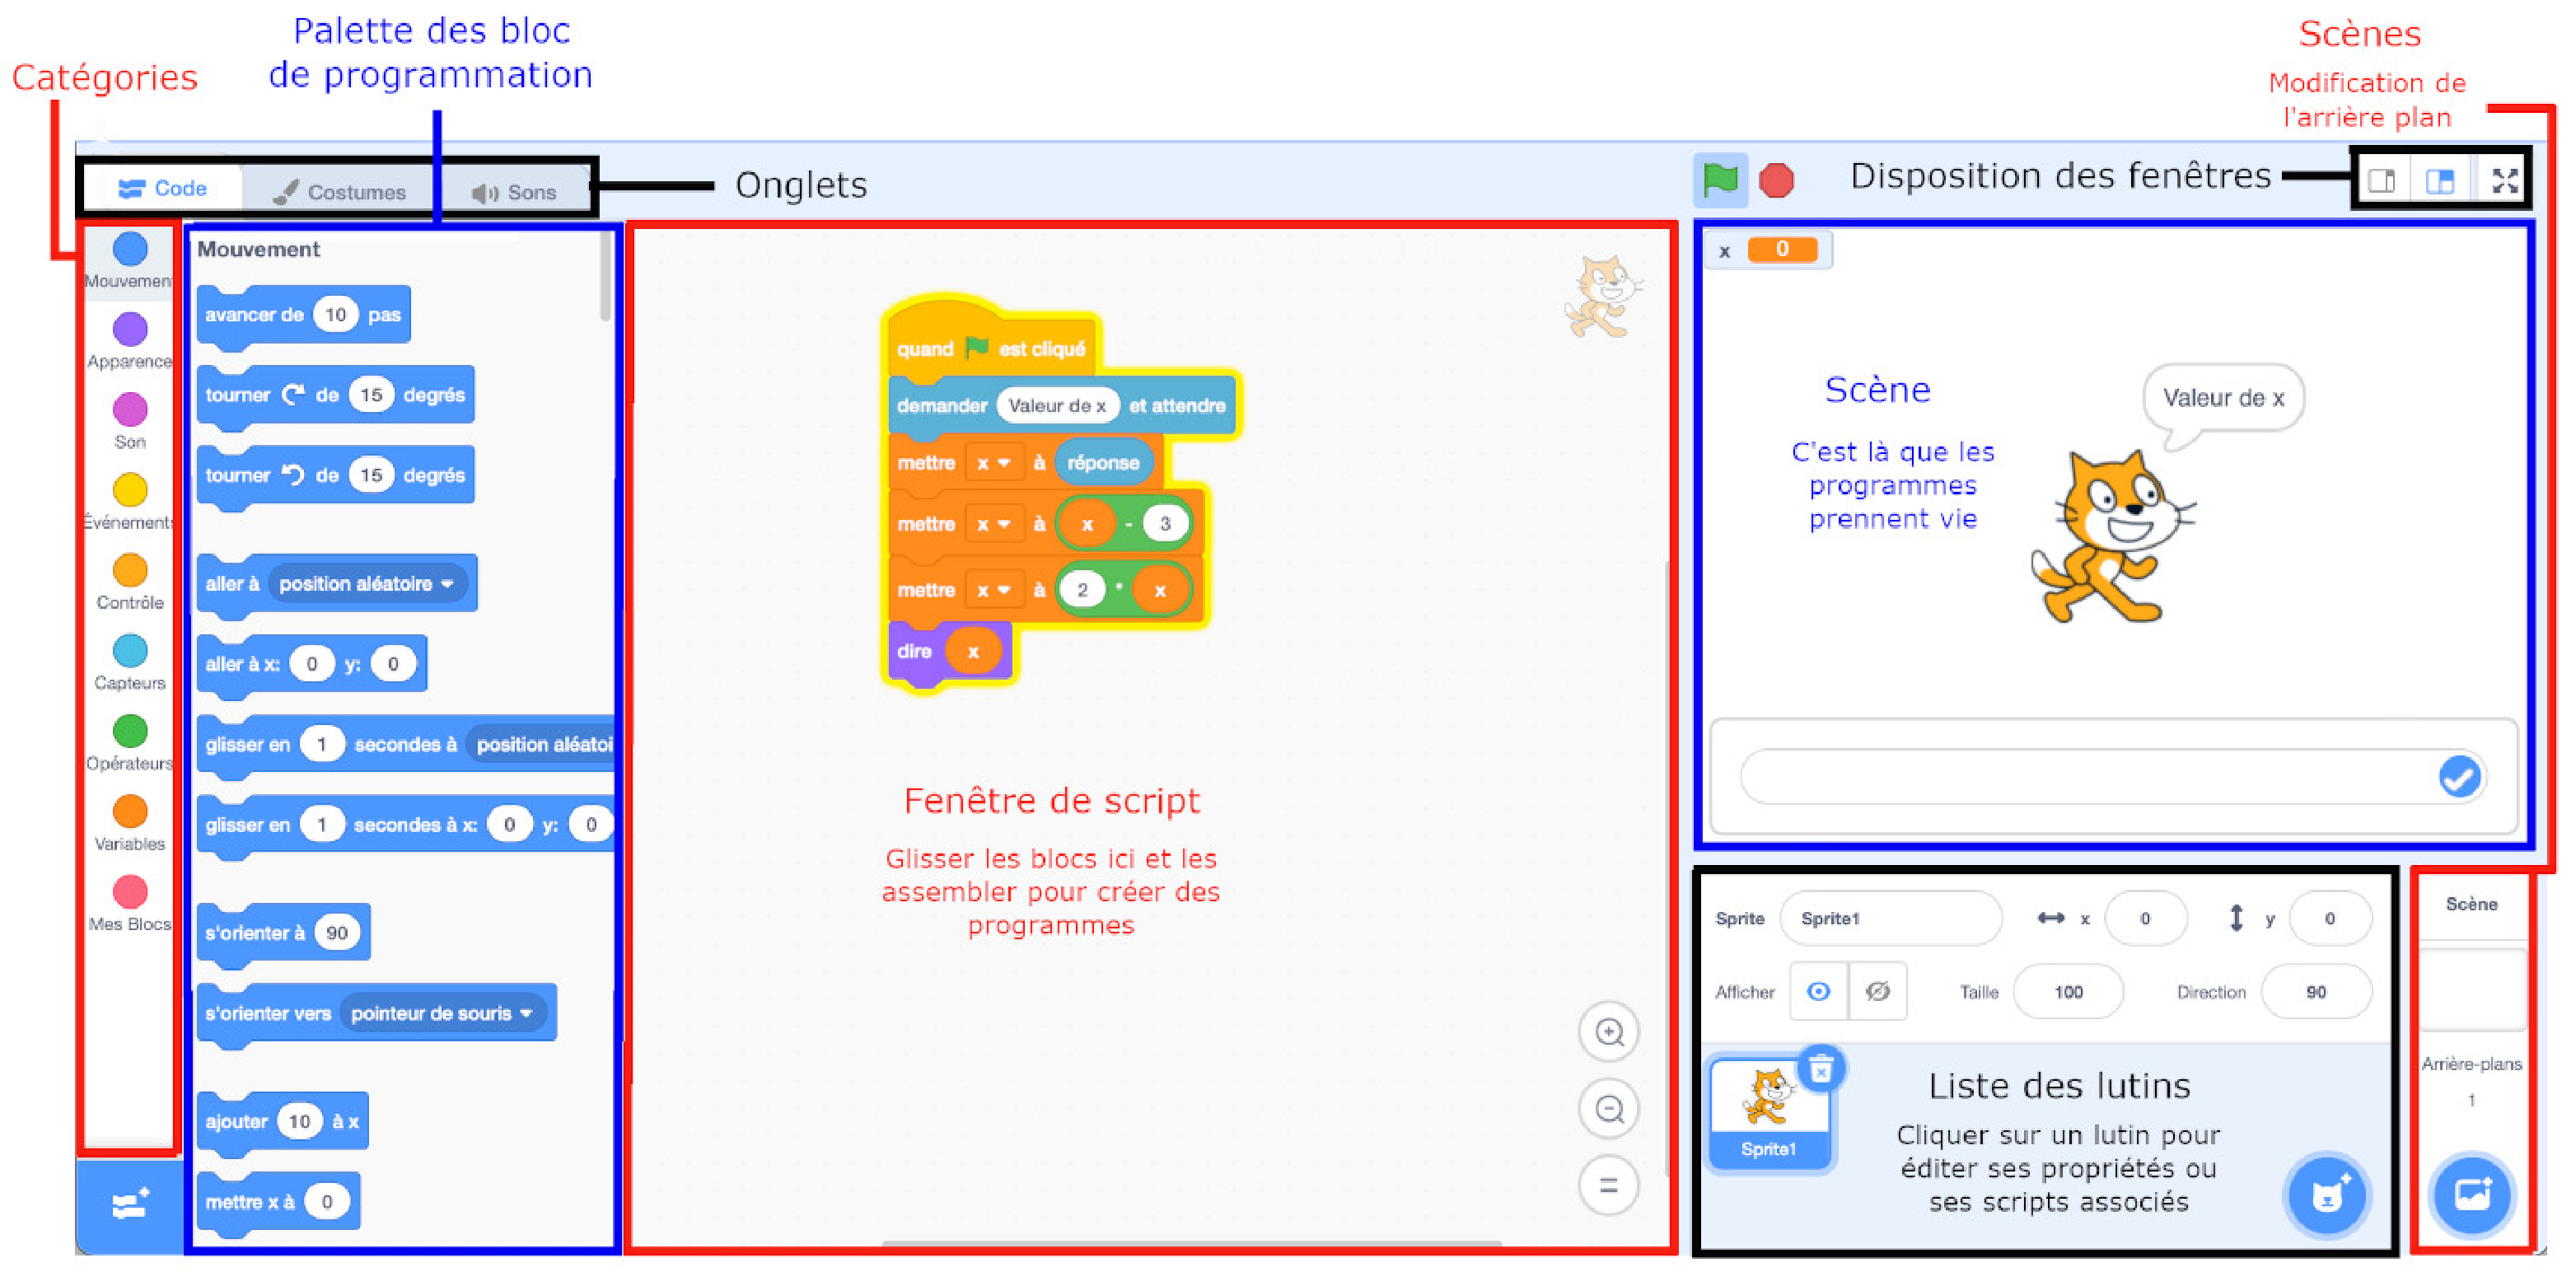
\includegraphics[width=16cm]{Interface_Scratch}
\end{center}


%%%%%%%%%%%
\section{Se déplacer}

\begin{methode}[Langages de déplacement]
   Pour se déplacer dans le plan, il existe principalement deux langages de déplacement :
   \begin{itemize}
      \item le langage {\bf absolu} composé de mots de vocabulaire du type : \og haut \fg{}, \og bas \fg{}, \og droite \fg{} et \og gauche \fg. Le déplacement se fait comme si on se plaçait en vue du dessus ;
      \item le langage {\bf relatif} composé de mots de vocabulaire du type : \og avancer \fg{}, \og tourner à droite \fg{} et \og tourner à gauche \fg. C'est ici le point de vue de l'observateur qui est adopté.
   \end{itemize}
   \exercice
   Coder ce déplacement :
   \begin{center}
   \psset{unit=0.6}
   \begin{pspicture}(0,0)(5,4)
      \psgrid[subgriddiv=1,gridlabels=0mm](0,-1)(5,4)
      \psset{linecolor=A1,arrowsize=3mm,linewidth=0.5mm}
      \psdots(0.5,0.5)(3.5,2.5)     
      \psline{->}(0.5,0.5)(2.5,0.5)(2.5,2.5)(3.5,2.5)
   \end{pspicture}
   \end{center}
   \correction
   \begin{minipage}{4cm}
      Avec le langage absolu : \\
      \og droite \\
      droite \\
      haut \\
      haut \\
      droite \fg \\ [5mm]
   \end{minipage}
   \qquad
   \begin{minipage}{4cm}   
     Avec le langage relatif : \\ [1mm]
     \og avancer \\
     avancer \\
     tourner à gauche \\
     avancer \\
     avancer \\
     tourner à droite \\
     avancer \fg
   \end{minipage}
\end{methode}


%%%%%%%%%%%%%%%%%%%%%%%%%%%%%%%%%%%%
%%%%%%%%%%%%%%%%%%%%%%%%%%%%%%%%%%%%
\exercicesbase

\begin{colonne*exercice}

\begin{exercice} %6
   Un programme permet à un robot de se déplacer sur les cases d'un quadrillage. Chaque case atteinte est colorée en gris. \\
Au début d'un programme, toutes les cases sont blanches, le robot se positionne sur une case de départ indiquée par un \og {\bf d} \fg{} et la colore aussitôt en gris. \\
Le robot se déplace suivant un programme grâce à un langage absolu dont le vocabulaire est
   \begin{center}
      \og S (south) ; E (east) ; N (north) ; W (west) \fg.
   \end{center}
   Voici des exemples de programmes et leurs effets :
   \begin{center}
   \begin{tabular}{|p{1.5cm}|C{2.5}|C{2.7}|}
      \hline
      1W
      &
      Le robot avance de 1 case vers l'ouest.
      &
      {\psset{unit=0.5cm}
      \begin{pspicture}(1,2)(3,3.5)
         \psframe[fillstyle=solid,fillcolor=lightgray](1,1)(3,2)
         \psgrid[gridlabels=0,subgriddiv=1,gridcolor=gray](0,0)(4,3)
         \rput(2.5,1.5){\textbf{d}}
      \end{pspicture}} \\
      \hline
      2E 1W 2N
      &
      Le robot avance de 2 cases vers l'est, puis de 1 case vers l'ouest,
puis de 2 cases vers le nord.
      &
      {\psset{unit=0.5cm}
      \begin{pspicture}(0,4.4)(5,6)
         \pspolygon[fillstyle=solid,fillcolor=lightgray](1,1)(4,1)(4,2)(3,2)(3,4)(2,4)(2,2)(1,2)
         \psgrid[gridlabels=0,subgriddiv=1,gridcolor=gray](5,5)
         \rput(1.5,1.5){\textbf{d}}
      \end{pspicture}} \\
      \hline
   \end{tabular}
   \end{center}
   \begin{enumerate}
      \item Voici un programme :
      \begin{center}
         1W 2N 2E 4S 2W
      \end{center}
      On souhaite dessiner le motif obtenu avec ce programme. Sur votre copie, réaliser ce motif en utilisant des carreaux, comme dans les exemples précédents. On marquera un \og \textbf{d} \fg{} sur la case de départ.
      \item On fait fonctionner un programme qui dessine le motif suivant :
      \begin{center}
      {\psset{unit=0.6cm}
      \begin{pspicture}(-0.5,-0.2)(8,3.7)
         \pspolygon[fillstyle=solid,fillcolor=lightgray](0,2)(1,2)(1,1)(2,1)(2,2)(3,2)(3,1)(4,1)(4,2)(5,2)(5,1)(6,1)(6,2)(7,2)(7,0)(0,0)
         \psgrid[gridlabels=0,subgriddiv=1,gridcolor=gray](-1,-1)(8,3)
         \rput(0.5,1.5){\textbf{d}}
      \end{pspicture}}
      \end{center}
      \begin{enumerate}
         \item Proposer un programme permettant de dessiner ce motif.
         \item Comment pourrait-on faire évoluer l'écriture de ce programme afin qu'il soit plus compact ?
      \end{enumerate}
   \end{enumerate}
   \end{exercice}

\begin{corrige}
   \ \\ [-5mm]\begin{enumerate}
      \item On obtient le {\blue dessin d'un 9} : \\
         {\psset{linecolor=white,fillstyle=solid,fillcolor=white}
         \begin{pspicture}(-1,0)(4,7.3)
            \psframe[fillcolor=lightgray](1,1)(4,6)
            \psframe(1,2)(3,3)          
            \psframe(2,4)(3,5)
            \psgrid[gridlabels=0,subgriddiv=1,gridcolor=gray](5,7)
            \rput(1.5,1.5){\textbf{d}}
         \end{pspicture}}
      \item \\
      \begin{enumerate}
         \item Le motif peut être programmé grâce à la suite : \\
            {\blue 1S 2E 1N 1S 2E 1N 1S 2E 1N}
         \item On peut introduire une boucle de répétition, par exemple : {\blue 3$\times$(1S 2E 1N)}
      \end{enumerate}
   \end{enumerate}
\end{corrige}


\begin{exercice} %2
   Tracer les figures obtenues lorsque l'on exécute les programmes suivants avec scratch. Pour chaque cas, donner la nature de la figure obtenue. \\
   {\it On représentera l'unité (un pas )par \umm{1} sur le cahier.} \\ [2mm]
         Programme 1 \hspace*{2.2cm} Programme 2 \\ [1mm]
         \begin{Scratch}[Echelle=0.7]
            Place Drapeau;
            Place PoserStylo;
            Place Repeter("4");
               Place Tournerd("90");
               Place Avancer("50");
            Place FinBlocRepeter;
         \end{Scratch}
         \qquad
         \begin{Scratch}[Echelle=0.7]
            Place Drapeau;
            Place PoserStylo;
            Place Repeter("3");
               Place Avancer("40");
               Place Tournerg("120");
            Place FinBlocRepeter;
         \end{Scratch}
         \\ [3mm]
         Programme 3 \hspace*{2.2cm} Programme 4 \\ [1mm]
         \begin{Scratch}[Echelle=0.7]
            Place Drapeau;
            Place PoserStylo;
            Place Repeter("2");
               Place Avancer("20");
               Place Tournerd("90");
               Place Avancer("80");
               Place Tournerd("90");
            Place FinBlocRepeter;
         \end{Scratch} 
         \qquad
         \begin{Scratch}[Echelle=0.7]
            Place Drapeau;
            Place PoserStylo;
            Place Repeter("2");
               Place Avancer("30");
               Place Tournerd("50");
               Place Avancer("30");
               Place Tournerd("130");
            Place FinBlocRepeter;
         \end{Scratch}
\end{exercice}

\begin{corrige}
   Le programme 1 donne un {\blue carré} de côté \ucm{5}, le programme 2 un {\blue triangle équilatéral} de côté \ucm{4}, le programme 3 un {\blue losange} de côté \ucm{3} et le programme 4 un {\blue rectangle} de longueur \ucm{8} et de largeur \ucm{2}. \\
   {\psset{linecolor=blue}
   \begin{pspicture}(0,0)(7,7.3)                                                                              
      \psgrid[gridlabels=0,subgriddiv=0,gridcolor=lightgray](0,0)(7,7)
      \psdot[linewidth=0.7mm](1,6)
      \psframe(1,1)(6,6)    
   \end{pspicture}}
   
\Coupe

   {\psset{linecolor=blue}
   \begin{pspicture}(0,0)(8,9)                                                                              
      \psgrid[gridlabels=0,subgriddiv=0,gridcolor=lightgray](0,0)(8,9)    
      \psdot[linewidth=0.7mm](0,4)
      \pspolygon(0,4)(4,4)(2,7.46)
      \psdot[linewidth=0.7mm](6,8)
      \psframe(6,0)(8,8)
      \psdot[linewidth=0.7mm](0,3)
      \pspolygon(0,3)(3,3)(4.93,0.7)(1.93,0.7)
   \end{pspicture}}
\end{corrige}


\begin{exercice} %3
   En utilisant les instructions ci-dessous, écrire un programme permettant de tracer les pointillés. \\
   \begin{pspicture}(0,-0.5)(10,0.5)
      \psline[linewidth=1mm,linecolor=blue](0,0)(1,0)
      \psline[linewidth=1mm,linecolor=blue](2,0)(3,0)
      \psline[linewidth=1mm,linecolor=blue](4,0)(5,0)
      \psline[linewidth=1mm,linecolor=blue](6,0)(7,0)
      \psline[linewidth=1mm,linecolor=blue](8,0)(9,0)
   \end{pspicture} \\
   \begin{Scratch}[Echelle=0.7]
      Place PoserStylo;
      Place LigneVide;
      Place Avancer("10");
      Place LigneVide;
      Place ReleverStylo;
   \end{Scratch} 
   \qquad
   \begin{Scratch}[Echelle=0.7]
      Place Drapeau;
      Place LigneVide;
      Place Repeter("");
         Place LigneVide;
      Place FinBlocRepeter;      
   \end{Scratch} \\
\end{exercice}

\begin{corrige}
   On peut proposer le programme suivant : \\ [1mm]
   \begin{Scratch}[Echelle=0.7]
      Place Drapeau;
      Place Repeter("5");
         Place PoserStylo;
         Place Avancer("10");
         Place ReleverStylo;
         Place Avancer("10");
      Place FinBlocRepeter;      
   \end{Scratch}
\end{corrige}


\begin{exercice}%4
   Proposer un programme permettant de dessiner les marches d'un escalier comme ci-dessous. \\
   Chaque segment de la marche doit mesurer 100 pas. \\
   {\psset{unit=0.5}
   \begin{pspicture}(-4,0)(6,6.5)
     \psline[linewidth=1mm,linecolor=blue](0,6)(0,4)(2,4)(2,2)(4,2)(4,0)(6,0)
   \end{pspicture}}
\end{exercice}

\begin{corrige}
   On peut proposer le programme suivant : \\ [1mm]
   \begin{Scratch}[Echelle=0.7]
      Place Drapeau;
      Place PoserStylo;
      Place Repeter("3");     
         Place Tournerd("90");
         Place Avancer("100");
         Place Tournerg("90");
         Place Avancer("100");
      Place FinBlocRepeter;      
   \end{Scratch}
\end{corrige}
   
   
\end{colonne*exercice}


%%%%%%%%%%%%%%%%%%%%%%%%%%%%%%%%%
%%%%%%%%%%%%%%%%%%%%%%%%%%%%%%%%%
\Recreation

\begin{enigme}[Le jeu des dominogrammes]
   
   {\bf But du jeu} : en groupe, faire une chaîne fermée avec les huit cartes de domino. \\ [1mm]
   {\bf Règle du jeu} : chaque domino est basé sur {\it Les douze travaux d'Hercule}, et notamment le travail n\degre11 dans lequel Hercule doit dérober les pommes d'or du jardin d'Hespérides. Le côté gauche comporte un quadrillage avec des cases noirs que l'on ne peut pas traverser, le personnage d'Hercule (orienté) et le pommier du jardin d'Hespérides. Le côté droit comporte un programme de déplacement d'Hercule. L'objectif est d'associer un programme d'un domino avec un quadrillage d'un autre domino. Les huit dominos doivent créer une chaine fermée. \\ [2mm]
   {\psset{unit=0.4}
   \begin{pspicture}(-1,-1)(19,10) % jaune 1
      \psframe(-1,-1)(19,9)
      \psline(9,-1)(9,9)
      \psgrid[subgriddiv=1,gridlabels=0](0,0)(8,8)
      \put(3.1,4.1){\ho} \put(7.1,6.1){\po}
      \put(1,1){\cn} \put(2,3){\cn} \put(3,2){\cn} \put(2,4){\cn}  \put(5,5){\cn} \put(7,2){\cn} \put(5,7){\cn} \put(6,0){\cn} \put(1,6){\cn}     
      \put(10,7){\dep}
      \put(10,6){\av{3}}
      \put(10,5){\td}
      \put(10,4){\av{1}}
      \put(10,3){\tg}
      \put(10,2){\av{1}}
      \put(10,1){\fin}
      \put(18,8){\ding{40}}
   \end{pspicture}
   \;
   \begin{pspicture}(-1,-1)(19,10) % jaune 2
      \psframe(-1,-1)(19,9)
      \psline(9,-1)(9,9)
      \psgrid[subgriddiv=1,gridlabels=0](0,0)(8,8)
      \rput{90}(3.5,2.5){\ho} \put(4.1,6.1){\po}
      \put(1,2){\cn} \put(4,3){\cn} \put(3,0){\cn} \put(2,7){\cn}  \put(5,6){\cn} \put(1,2){\cn} \put(0,7){\cn} \put(6,2){\cn} \put(1,3){\cn}     
      \put(10,7){\dep}
      \put(10,6){\td}
      \put(10,5){\av{4}}
      \put(10,4){\tg}
      \put(10,3){\av{3}}
      \put(10,2){\tg}
      \put(10,1){\av{1}}
      \put(10,0){\fin}
      \put(18,8){\ding{110}}
   \end{pspicture}

   \medskip
   \begin{pspicture}(-1,-1)(19,9) % jaune 3
      \psframe(-1,-1)(19,9)
      \psline(9,-1)(9,9)
      \psgrid[subgriddiv=1,gridlabels=0](0,0)(8,8)
      \put(5.1,3.1){\reflectbox{\ho}} \put(2.1,6.1){\po}
      \put(6,6){\cn} \put(3,3){\cn} \put(3,6){\cn} \put(2,5){\cn}  \put(3,5){\cn} \put(4,2){\cn} \put(1,3){\cn} \put(0,0){\cn} \put(2,5){\cn}     
      \put(10,7){\dep}
      \put(10,6){\av{7}}
      \put(10,5){\tg}
      \put(10,4){\av{7}}
      \put(10,3){\tg}
      \put(10,2){\av{7}}
      \put(10,1){\fin}
      \put(18,8){\ding{57}}
   \end{pspicture}
   \;
   \begin{pspicture}(-1,-1)(19,9) % jaune 4
      \psframe(-1,-1)(19,9)
      \psline(9,-1)(9,9)
      \psgrid[subgriddiv=1,gridlabels=0](0,0)(8,8)
      \put(0.1,0.1){\ho} \put(0.1,7.1){\po}
      \put(5,3){\cn} \put(4,3){\cn} \put(3,6){\cn} \put(0,6){\cn}  \put(5,5){\cn} \put(2,1){\cn} \put(2,5){\cn} \put(6,2){\cn} \put(1,3){\cn}     
      \put(10,7){\dep}
      \put(10,6){\av{3}}
      \put(10,5){\tg}
      \put(10,4){\td}
      \put(10,3){\av{2}}
      \put(10,2){\tg}
      \put(10,1){\av{2}}
      \put(10,0){\fin}
      \put(18,8){\ding{52}}
   \end{pspicture}

   \medskip
   \begin{pspicture}(-1,-1)(19,9) % jaune 5
      \psframe(-1,-1)(19,9)
      \psline(9,-1)(9,9)
      \psgrid[subgriddiv=1,gridlabels=0](0,0)(8,8)
      \rput{90}(5.5,0.5){\ho} \put(3.1,5.1){\po}
      \put(1,1){\cn} \put(0,3){\cn} \put(4,2){\cn} \put(3,4){\cn}  \put(5,6){\cn} \put(7,3){\cn} \put(5,7){\cn} \put(6,1){\cn} \put(1,7){\cn}     
      \put(10,7){\dep}
      \put(10,6){\av{6}}
      \put(10,5){\td}
      \put(10,4){\av{3}}
      \put(10,3){\td}
      \put(10,2){\av{2}}
      \put(10,1){\tg}
      \put(10,0){\fin}
      \put(18,8){\ding{70}}
   \end{pspicture}
   \;
   \begin{pspicture}(-1,-1)(19,9) % jaune 6
      \psframe(-1,-1)(19,9)
      \psline(9,-1)(9,9)
      \psgrid[subgriddiv=1,gridlabels=0](0,0)(8,8)
      \rput{-90}(4.5,7.5){\ho} \put(1.1,3.1){\po}
      \put(0,2){\cn} \put(6,5){\cn} \put(1,0){\cn} \put(2,0){\cn}  \put(3,6){\cn} \put(1,6){\cn} \put(6,7){\cn} \put(6,2){\cn} \put(1,7){\cn}     
      \put(10,7){\dep}
      \put(10,6){\av{2}}
      \put(10,5){\tg}
      \put(10,4){\av{1}}
      \put(10,3){\fin}
      \put(18,8){\ding{74}}
   \end{pspicture}

   \medskip
   \begin{pspicture}(-1,-1)(19,9) % jaune 7
      \psframe(-1,-1)(19,9)
      \psline(9,-1)(9,9)
      \psgrid[subgriddiv=1,gridlabels=0](0,0)(8,8)
      \put(7.1,7.1){\reflectbox{\ho}} \put(5.1,6.1){\po}
      \put(6,6){\cn} \put(2,3){\cn} \put(0,6){\cn} \put(4,2){\cn}  \put(3,7){\cn} \put(1,2){\cn} \put(0,3){\cn} \put(7,2){\cn} \put(2,5){\cn}
      \put(10,7){\dep}
      \put(10,6){\av{2}}
      \put(10,5){\tg}
      \put(10,4){\tg}
      \put(10,3){\tg}
      \put(10,2){\tg}
      \put(10,1){\av{2}}
      \put(10,0){\fin}
      \put(18,8){\ding{87}}
   \end{pspicture}
   \;
   \begin{pspicture}(-1,-1)(19,9) % jaune 8
      \psframe(-1,-1)(19,9)
      \psline(9,-1)(9,9)
      \psgrid[subgriddiv=1,gridlabels=0](0,0)(8,8)
      \rput{90}(2.5,3.5){\ho} \put(2.1,7.1){\po}
      \put(5,3){\cn} \put(3,3){\cn} \put(3,6){\cn} \put(0,5){\cn}  \put(7,5){\cn} \put(2,1){\cn} \put(2,0){\cn} \put(6,2){\cn} \put(1,3){\cn}     
   \put(10,7){\dep}
      \put(10,6){\av{1}}
      \put(10,5){\tg}
      \put(10,4){\av{2}}
      \put(10,3){\td}
      \put(10,2){\av{2}}
      \put(10,1){\av{1}}
      \put(10,0){\fin}
      \put(18,8){\ding{115}}
   \end{pspicture}}
   \\ [2mm]
   Lorsque le groupe a réussi la mission, passer au niveau supérieur avec une autre série de dominos comportant des boucles de répétition. 
\end{enigme}

\begin{corrige}
   Suite des dominos :\\    
   \ding{40} -- \ding{110} -- \ding{57} -- \ding{52} -- \ding{70} -- \ding{74} -- \ding{87} -- \ding{115}
\end{corrige}

\themaN
\graphicspath{{../../S04_Nombres_relatifs/Images/}}

\chapter{Nombres relatifs}
\label{S04}


%%%%%%%%%%%%%%%%%%%%%%%%%%%%%%%%%
%%%%%%%%%%%%%%%%%%%%%%%%%%%%%%%%%
\begin{autoeval}
   \small
   \begin{enumerate}
      \item Il utilise la notion d'opposé.
      \item Il repère sur une droite graduée les nombres décimaux relatifs.
      \item Il résout des problèmes faisant intervenir des nombres décimaux relatifs.
   \end{enumerate}
\end{autoeval}

\begin{prerequis}
   \begin{itemize}
      \item Nombres décimaux négatifs, notion d'opposé.
      \item[\com] Comparer, ranger, encadrer des nombres en écriture décimale.
   \end{itemize}
\end{prerequis}

\vfill

\def\thermo{\pspolygon[linearc=0.1,fillstyle=solid](-0.1,6.8)(-0.1,0.6)(-0.2,0.4)(-0.2,-0.1)(0.2,-0.1)(0.2,0.4)(0.1,0.6)(0.1,6.8) \pspolygon[linecolor=B1, linearc=0.1, fillstyle=solid, fillcolor=B1](0,5)(0,0.5)(-0.1,0.3)(-0.1,0)(0.1,0)(0.1,0.3)(0,0.5) \pscircle(0,6.7){0.05}}
            
\begin{debat}[Débat : les unités de mesure de température]
   Il existe trois échelles principales de température :
   \begin{itemize}
      \item l'échelle Farenheit, créée en 1720 par le scientifique allemand {\bf Gabriel Farenheit} et allant de \udeg{32}F à \udeg{212}F ;
      \item l'échelle Celsius, créée en 1741 par le physicien suédois {\bf Anders Celsius}  dans laquelle \udeg{0}C correspond au point de congélation de l'eau et \udeg{100}C à son point d'ébullition ;
      \item l'échelle de Kelvin, créée à la fin du {\small XIX}\up{e} siècle par {\bf Lord Kelvin} pour laquelle le point 0 correspond au zéro absolu, c'est-à-dire à la plus basse température existante.
   \end{itemize}
   \begin{center}
      {\psset{yunit=0.6}
      \begin{pspicture}(0,0)(8,7)
         \textcolor{B1}{
         \rput(1,0){\thermo}
         \rput[l](1.2,1){\udeg{-459}F}
         \rput[l](1.2,6){\udeg{212}F}
         \rput[l](1.2,4.66){\udeg{32}F}
         \rput(3.5,0){\thermo}
         \rput[l](3.7,1){\udeg{-273}C} 
         \rput[l](3.7,4.66){\udeg{0}C}
         \rput[l](3.7,6){\udeg{100}C}
         \rput(6,0){\thermo}
         \rput[l](6.2,1){\udeg{0}K} 
         \rput[l](6.2,4.66){\udeg{273}K}  
         \rput[l](6.2,6){\udeg{373}K} }          
      \end{pspicture}}
   \end{center}
   \bigskip
   \begin{cadre}[B2][J4]
      \begin{center}
         Vidéo : \href{https://www.youtube.com/watch?v=nzirDkQN99M}{\bf Celsius et Farenheit}, chaîne YouTube {\it Ma deuxième école}, épisode de la série {\it Culture G}.
      \end{center}
   \end{cadre}
\end{debat}


%%%%%%%%%%%%%%%%%%%%%%%%%%%%%%%%
%%%%%%%%%%%%%%%%%%%%%%%%%%%%%%%%
\activites

\begin{activite}[Carrés magiques]
   {\bf Objectifs : } résoudre un problème avec des nombres ; montrer que, pour résoudre un problème, il est parfois nécessaire d’inventer de nouveaux nombres, des nombres négatifs.
   \begin{QCM}
      \begin{minipage}{10cm}
         Un carré magique est un tableau carré tel que la somme pour chaque ligne, chaque colonne et chaque diagonale soit la même.
      \end{minipage}
      \qquad
      \begin{minipage}{5cm}
         \begin{pspicture}(-0.5,-1.5)(4,3.25)
            \psgrid[griddots=50, subgriddiv=0, gridlabels=0](0,0)(3,3)
            \rput(0.5,0.5){4}
            \rput(1.5,0.5){3}
            \rput(2.5,0.5){8}
            \rput(0.5,1.5){9}
            \rput(1.5,1.5){5}
            \rput(2.5,1.5){1}
            \rput(0.5,2.5){2}
            \rput(1.5,2.5){7}
            \rput(2.5,2.5){6}
            \rput(0.5,-0.3){$\downarrow$}
            \rput(0.5,-0.7){15}
            \rput(1.5,-0.3){$\downarrow$}
            \rput(1.5,-0.7){15}
            \rput(2.5,-0.3){$\downarrow$}
            \rput(2.5,-0.7){15}
            \rput(3.3,0.5){$\rightarrow$}
            \rput(3.7,0.5){15}
            \rput(3.3,1.5){$\rightarrow$}
            \rput(3.7,1.5){15}
            \rput(3.3,2.5){$\rightarrow$}
            \rput(3.7,2.5){15}
            \rput(3.3,-0.3){$\searrow$}
            \rput(3.7,-0.7){15}
            \rput(-0.3,-0.3){$\swarrow$}
            \rput(-0.7,-0.7){15}
         \end{pspicture}
      \end{minipage} \\
      Compléter les carrés suivants pour les rendre magiques en commençant par déterminer la somme commune.
      \begin{center}
      {\psset{unit=1.5,griddots=50, subgriddiv=0, gridlabels=0}
      \large
         \begin{pspicture}(0,-0.3)(4,4)
            \psgrid(0,0)(3,3)
            \rput(0.5,0.5){4}
            \rput(0.5,2.5){8}
            \rput(1.5,1.5){5}
            \rput(2.5,0.5){2}
            \rput(1.4,3.5){Somme = \pointilles[15mm]}
         \end{pspicture}
         \begin{pspicture}(-1,-0.3)(3,4)
            \psgrid(0,0)(3,3)
            \rput(2.5,2.5){24}
            \rput(0.5,2.5){18}
            \rput(1.5,1.5){15}
            \rput(2.5,0.5){12}
            \rput(1.4,3.5){Somme = \pointilles[15mm]}
         \end{pspicture}
      
          \begin{pspicture}(0,-0.3)(4,4)
            \psgrid(0,0)(3,3)
            \rput(1.5,2.5){7}
            \rput(0.5,2.5){2}
            \rput(1.5,1.5){3}
            \rput(2.5,0.5){4}
            \rput(1.4,3.5){Somme = \pointilles[15mm]}
         \end{pspicture}
         \begin{pspicture}(-1,-0.3)(3,4)
            \psgrid(0,0)(3,3)
            \rput(2.5,2.5){4}
            \rput(0.5,0.5){10}
            \rput(1.5,1.5){7}
            \rput(1.5,2.5){1}
            \rput(1.4,3.5){Somme = \pointilles[15mm]}
         \end{pspicture}}
      \end{center}   
   \end{QCM}
   \vfill\hfill{\footnotesize\it Source : Une introduction des nombres relatifs en 5\up{e} - PLOT 45, APMEP 2014.}
\end{activite}


%%%%%%%%%%%%%%%%%%%%%%%%%%%%%%%%
%%%%%%%%%%%%%%%%%%%%%%%%%%%%%%%%
\cours 

%%%%%%%%%%%%%
\section{Nombres relatifs}

\begin{definition}
   Un {\bf nombre relatif} est un nombre positif ($+$) ou négatif ($-$). Le nombre sans son signe correspond à sa distance à l'origine 0.
\end{definition}

\begin{exemple*1}
   Les étages d'un immeuble sont  repérés par rapport à un niveau 0 : le rez-de-chaussée. Les étages au-dessus sont les étages positifs et les étages en dessous (cave, garages) sont les étages négatifs.
\end{exemple*1}

\begin{exemple*1}
   Le signe de $+3$ est $+$ et sa distance à l'origine 0 est 3. \\
   Le signe de $-7$ est $-$ et sa distance à l'origine 0 est 7.  
\end{exemple*1}

\medskip

\begin{definition}
   L'{\bf opposé} d'un nombre relatif est le nombre de signe contraire et de même	
distance à 0.
\end{definition}

\begin{exemple*1}
   L'opposé de $-3$ est $+3$ et l'opposé de $+2$ est $-2$ .
\end{exemple*1}

\begin{remarque}
   de manière usuelle, on omet le signe \og $+$ \fg{} devant les nombres positifs.
\end{remarque}


%%%%%%%%%%%%%%%%%%%%
\section{Droite graduée et comparaison}

\begin{definition}
   Sur une droite graduée, on repère chaque point par un nombre : son abscisse. \\
   D'un côté de l'origine 0, on place les nombres négatifs et de l'autre les nombres positifs.
   \begin{center}
      \begin{pspicture}(-5,-0.5)(5,0.8)
         \psaxes[yAxis=false]{->}(0,0)(-5,0)(5,0)
         \psline[linecolor=B1]{<->}(-5,0.3)(0,0.3)
         \rput(-2.5,0.6){\textcolor{B1}{nombres négatifs}}
         \psline[linecolor=A1]{<->}(0,0.3)(5,0.3)
         \rput(2.5,0.6){\textcolor{A1}{nombres positifs}}
      \end{pspicture}
   \end{center}
\end{definition}

\medskip

\begin{exemple*1}
   L'abscisse de A est $-3$, on note A($-3$) ; l'abscisse de B est , l'abscisse de C est $+4$.
   \begin{center}
      \begin{pspicture}(-5,-0.5)(5,0.5)
         \psaxes[yAxis=false]{->}(0,0)(-5,0)(5,0)
         \rput(-3,0.5){A}
         \rput(0,0.5){B}
         \rput(4,0.5){C}
         \psline[linecolor=B1]{<->}(-3,-0.9)(0,-0.9)
         \rput(-1.5,-1.2){\textcolor{B1}{\small distance à l'origine : 3}}
         \psline[linecolor=A1]{<->}(0,-0.9)(4,-0.9)
         \rput(2,-1.2){\textcolor{A1}{\small distance à l'origine : 4}}
      \end{pspicture}
   \end{center}
\end{exemple*1}

\medskip

\begin{propriete}
   \begin{itemize}
      \item Deux nombres relatifs négatifs sont rangés dans l'ordre inverse de leur
distance à zéro.
      \item Un nombre relatif négatif est inférieur à un nombre relatif positif.
      \item Deux nombres relatifs positifs sont rangés dans l'ordre de leur distance à zéro. \\ [-8mm]
   \end{itemize}  
\end{propriete}

\begin{exemple*1}
   $-4<-2$ car $4>2$ \qquad ; \quad $-4<2$ car $-4<0$ et $2>0$ \qquad ; \quad $+4>+2$ car $4>2$.
\end{exemple*1}

\medskip

\begin{remarque}
   les nombres négatifs sont rangés \og dans le sens inverse \fg{} des nombres positifs.
\end{remarque}


%%%%%%%%%%%%%%%%%%%%%%%%%%%%%%
%%%%%%%%%%%%%%%%%%%%%%%%%%%%%%
\exercicesbase

\begin{colonne*exercice}

\begin{exercice} %1
   Quelle est la température indiquée par chacun des thermomètres ? \\ [3mm]
   \hspace*{-5mm}
      \Reperage[Thermometre,Pasx=10,ValeurUnitex=5,Mercure]{4/A,-16/,16/}
   \Reperage[Thermometre,Pasx=10,ValeurUnitex=10,Mercure]{-12/A,-15/,17/}
   \Reperage[Thermometre,Pasx=5,Mercure]{-2/A,-10/,6/}
   \Reperage[ Thermometre,Pasx=5,ValeurUnitex=0.5,Mercure]{7/A,-5/,11/}
\end{exercice}

\begin{corrige}
   On peut lire les températures suivantes : \\
   \blue \udegc{2} \hfill \udegc{-12} \hfill \udegc{-0,4} \hfill \udegc{0,7}
\end{corrige}

\bigskip


\begin{exercice} %2
   Colorier les thermomètres jusqu'à la graduation correspondant à la température donnée. \\ [3mm]
   \Reperage[Thermometre,Pasx=10,ValeurUnitex=10]{-17/A,-15/,15/}
   \Reperage[Thermometre,Pasx=5,ValeurUnitex=1]{-6/,-10/,6/}
   \Reperage[ Thermometre,Pasx=10,ValeurUnitex=1]{-5/,-20/,12/}
   \Reperage[ Thermometre,Pasx=10,ValeurUnitex=5]{12/,-15/,17/} \\
   \hspace*{10mm} $-17$ \hfill $-1,2$ \hfill $-0,5$ \hfill $6$
\end{exercice}

\begin{corrige}
   On a les hauteurs de mercure suivantes : \\ [2mm]
   \hspace*{-15mm}
   \Reperage[Thermometre,Pasx=10,ValeurUnitex=10,Mercure]{-17/A,-15/,15/}
   \Reperage[Thermometre,Pasx=5,ValeurUnitex=1,Mercure]{-6/,-10/,6/}
   \Reperage[ Thermometre,Pasx=10,ValeurUnitex=1,Mercure]{-5/,-20/,12/}
   \Reperage[ Thermometre,Pasx=10,ValeurUnitex=5,Mercure]{12/,-15/,17/} \\
\end{corrige}

\bigskip


\begin{exercice} %3
   Entourer en bleu les nombres positifs et en rouge les nombres négatifs.
   \begin{center}
       {\hautab{2}
       \begin{tabular}{|*{5}{C{1}|}}
         \hline
         $12$ & $+\pi$ & $-\dfrac{12}{13}$ & $-17$ & $+0,001$ \\
         \hline
         $-54,2$ & $\dfrac{1}{10}$ & $-0,14$ & $\dfrac{3}{7}$ & $100,01$ \\
         \hline
         $12,6$ & $-1,18$ & $-3^2$ & $0,1$ & $48\,000$ \\
         \hline
      \end{tabular}}
   \end{center}
\end{exercice}

\begin{corrige}
   \ \\ [-3mm]
   {\hautab{1.8}
      \begin{tabular}{|*{5}{C{1.05}|}}
         \hline
         \fcolorbox{blue}{white}{$12$} & \fcolorbox{blue}{white}{$+\pi$} & \fcolorbox{red}{white}{$-\dfrac{12}{13}$} & \fcolorbox{red}{white}{$-17$} & \!\!\fcolorbox{blue}{white}{$+0,001$} \\
         \hline
         \fcolorbox{red}{white}{$-54,2$} & \fcolorbox{blue}{white}{$\dfrac{1}{10}$} & \fcolorbox{red}{white}{$-0,14$} & \fcolorbox{blue}{white}{$\dfrac{3}{7}$} & \fcolorbox{blue}{white}{$100,01$} \\
         \hline
         \fcolorbox{blue}{white}{$12,6$} & \fcolorbox{red}{white}{$-1,18$} & \fcolorbox{red}{white}{$-3^2$} & \fcolorbox{blue}{white}{$0,1$} & \fcolorbox{blue}{white}{$48\,000$} \\
         \hline
      \end{tabular}}
\end{corrige}

\bigskip


\begin{exercice} %4
   Compléter le tableau suivant :
   \begin{center}
      {\hautab{1.3}
      \begin{Ctableau}{0.95\linewidth}{7}{c}
         \hline
         Nombre & 2,5 & & \; 0 & $-5$ & & 7,1 \\
         \hline
         Opposé & & \!\!$-2,7$ & & & \; 1 & \\
         \hline 
      \end{Ctableau}}
   \end{center}
\end{exercice}

\begin{corrige}
   \ \\ [-3mm]
      {\hautab{1.3}
      \begin{Ctableau}{1\linewidth}{7}{c}
         \hline
         Nombre & \,2,5 & \,\textcolor{blue}{2,7} & \; 0 & $-5$ & \textcolor{blue}{$-1$} & \,7,1 \\
         \hline
         Opposé & \!\!\textcolor{blue}{$-2,5$} & \!\!$-2,7$ & \; \textcolor{blue}{0} & \; \textcolor{blue}{5} & \; 1 & \!\!\textcolor{blue}{$-7,1$} \\
         \hline 
      \end{Ctableau}}
\end{corrige}

\bigskip


\begin{exercice} %5
   Reproduire l'axe chronologique ci-dessous puis placer le plus précisément possible ces évènements : \\ [2mm]
   \Reperage[Unitex=0.75,ValeurUnitex=100]{4/B,-5/A}
   \begin{itemize}
      \item T : le temple de Jérusalem est détruit en 70 après Jésus-Christ ;
      \item J : Jules César naît en 100 avant J.-C. ;
      \item C : Constantin crée Constantinople en 324 ;
      \item A : Alexandre le Grand meurt en 324 avant J.-C.
   \end{itemize}
\end{exercice}

\begin{corrige}
   Droite graduée complétée : \\ [2mm]
   \hspace*{-10mm} \Reperage[Unitex=0.75,ValeurUnitex=100,AffichageNom,AffichageAbs=1]{-5/,-1/J,0.7/T,3.24/C,-3.24/A,4/}
\end{corrige}

\medskip


\begin{exercice} %6 
   Construire une droite graduée dont l'origine est au milieu du cahier et l'unité vaut \ucm{1} puis répondre aux questions suivantes.
   \begin{enumerate}
      \item Sur la droite graduée, placer les points : \\
         A($+8$), B($-2$), C($+3$), D($-5$) et E($+2$).
      \item En examinant la position des points A, B, C, D et E sur cette droite graduée, comparer : \\ [-9mm]
         \begin{multicols}{3}
            $+2$ et $-2$ \\ \smallskip
            $-2$ et $-5$ \\ \smallskip
            $+2$ et $-5$ \\
            $+8$ et $-2$ \\
            $+3$ et $+8$ \\
            $-5$ et $+3$
         \end{multicols}
         \ \\ [-15mm]
      \item Ranger dans l'ordre croissant : $+8 ; -2 ; +3 ; -5$ et $+2$.
   \end{enumerate}
\end{exercice}

\begin{corrige}
   \ \\ [-5mm]
   \begin{enumerate}
      \item Droite graduée complétée (à l'échelle 1/2) : \\ [2mm]
      \hspace*{-10mm} \Reperage[Unitex=0.5,AffichageNom,AffichageAbs=1]{-6/,-5/D,-2/B,2/E,3/C,8/A,9/}
      \item On peut comparer directement par lecture graphique :
         \begin{multicols}{3}
            $+2 \; {\blue >} \, -2$ \\ \smallskip
            $-2  \; {\blue >} \, -5$ \\ \smallskip
            $+2 \; {\blue >} \, -5$ \\
            $+8 \; {\blue >} \, -2$ \\
            $+3 \; {\blue <} \, +8$ \\
            $-5 \; {\blue <} \, +3$
         \end{multicols}
         \vspace*{-3mm}
      \item \blue$-5<-2<+2<+3<+8$.
   \end{enumerate}
\end{corrige}

\medskip


\begin{exercice} %7
   Compléter par <, > ou =.
   {\baselineskip=7mm
   \begin{colenumerate}{2} 
      \item $+5,34 \pointilles +3,54$
      \item $0,05 \pointilles 1$
      \item $-8,51 \pointilles -8,5$
      \item $11,9 \pointilles +11,9$
      \item $3,14 \pointilles -1,732$
      \item $-9,27 \pointilles -9,272$
      \item $+8,64 \pointilles -8,64$
      \item $-19,2 \pointilles +9,2$
      \item $-14,39 \pointilles +14,4$
      \item $-0,99 \pointilles -0,909$
   \end{colenumerate}}
\end{exercice}

\begin{corrige}
   \ \\ [-7mm]
   {\baselineskip=7mm
   \begin{colenumerate}{2}
      \item $+5,34 \; {\blue >} \, +3,54$
      \item $0,05 \; {\blue <} \, 1$
      \item $-8,51 \; {\blue <} \, -8,5$
      \item $11,9 \; {\blue =} \, +11,9$
      \item $3,14 \; {\blue >} \, -1,732$
      \item $-9,27 \; {\blue >} \, -9,272$
      \item $+8,64 \; {\blue >} \, -8,64$
      \item $-19,2 \; {\blue <} \, +9,2$
      \item $-14,39 \; {\blue <} \, +14,4$
      \item $-0,99 \; {\blue <} \, -0,909$
   \end{colenumerate}}
\end{corrige}

\medskip


\begin{exercice} %8
   Ranger dans l'ordre croissant et simplifier.
   {\baselineskip=7mm
   \begin{enumerate}
      \item $+3 \; ; \; -7 \;;\;-8 \;;\; +7 \;; \;+14\; ;\; +8 \;;\; -9$.
      \item $+5,0\; ; \;+2,7 \;;\; -2,6\; ; \;-3,1\; ; \;+7,1\; ; \;-8,3\; ;\; -0,2$.
      \item $-10,6 \;; \;+14,52\; ;\; -8,31 \;; \;-3,8 \;; \;+4,2 \;; \;+14,6\; ;\; -8,3$.
   \end{enumerate}}  
\end{exercice}

\begin{corrige}
   \ \\ [-7mm]
   {\baselineskip=7mm
   \begin{enumerate}
      \item \blue $-9<-8<-7<+3<+7<+8<+14$.
      \item \blue $-8,3<-3,1<-2,6<-0,2<2,7<5<7,1$.
      \item \blue$-10,6<-8,31<-8,3<-3,8<4,2<14,52$ \\
      \hfill $<14,6$.
   \end{enumerate}}  
\end{corrige}

\medskip


\begin{exercice} %8
   Chasser l'intrus dans chacun des cas suivants.
   {\baselineskip=7mm
   \begin{enumerate}
      \item $-9,84 < -9,72 < -9,67 < -9,78 < -9,18$
      \item $+1,5 < +1,51 < +1,499 < +1,54 < +1,55$
      \item $-1\,002 > -1\,220 > -1\,022 > -1\,202 > -1\,222$
   \end{enumerate}}
\end{exercice}

\begin{corrige}
   \ \\ [-7mm]
   {\baselineskip=7mm
   \begin{enumerate}
      \item $-9,84 < -9,72 < -9,67 < {\blue\cancel{-9,78}} < -9,18$ 
      \item $+1,5 < +1,51 < {\blue\cancel{+1,499}} < +1,54 < +1,55$ 
      \item $-1\,002 > {\blue\cancel{-1\,220}} > -1\,022 > -1\,202 > -1\,222$
   \end{enumerate}}
\end{corrige}

\medskip


\begin{exercice} %10
   Donner tous les entiers relatifs compris entre :
   \begin{colenumerate}{2}
      \item $-2,3$ et $+5,7$.
      \item $-20$ et $-14,8$.
   \end{colenumerate}
\end{exercice}

\begin{corrige}
   \ \\ [-5mm]
   \begin{enumerate}
      \item Entre $-2$ et $+5$ : {\blue$-1 \; ; \; 0 \; ; \; 1 \; ; \; 2 \; ; \; 3 \; ; \; 4$}. \smallskip
      \item Entre $-15$ et $-20$ : {\blue $-19 \; ; \; -18 \; ; \; -17 \; ; \; -16$}. \smallskip
   \end{enumerate}
\end{corrige}

\end{colonne*exercice}


%%%%%%%%%%%%%%%%%%%%%%%
%%%%%%%%%%%%%%%%%%%%%%
\Recreation

\begin{enigme}[Nombres croisés]
   Compléter cette grille de nombres croisés à l'aide de chiffres et de signes \og $+$ \fg{} ou \og $-$ \fg{} grâce aux indications données.
   \begin{center}
   {\hautab{1.95}
   \begin{tabular}{|*{7}{C{0.57}|}}
      \hline
      & \cellcolor{J2}{\textcolor{B1}{a}} & \cellcolor{J2}{\textcolor{B1}{b}} & \cellcolor{J2}{\textcolor{B1}{c}} & \cellcolor{J2}{\textcolor{B1}{d}} & \cellcolor{J2}{\textcolor{B1}{e}} & \cellcolor{J2}{\textcolor{B1}{f}} \\
      \hline
      \cellcolor{J2}{\textcolor{A1}{1}} & & \cellcolor{black!70} & & & \cellcolor{black!70} & \\
      \hline
      \cellcolor{J2}{\textcolor{A1}{2}} & & & & \cellcolor{black!70} & & \\
      \hline
      \cellcolor{J2}{\textcolor{A1}{3}} & & \cellcolor{black!70} & \cellcolor{black!70} & & & \cellcolor{black!70} \\
      \hline
      \cellcolor{J2}{\textcolor{A1}{4}} & \cellcolor{black!70} & & & \cellcolor{black!70} & \cellcolor{black!70} & \\
      \hline
      \cellcolor{J2}{\textcolor{A1}{5}} & & & \cellcolor{black!70} & & & \\
      \hline
      \cellcolor{J2}{\textcolor{A1}{6}} & & \cellcolor{black!70} & & & & \cellcolor{black!70} \\
      \hline
   \end{tabular}}
   \end{center}
   \bigskip
   \begin{multicols}{2}
   {\bf Horizontalement} \\
   \begin{enumerate}
      \item Valeur du plus grand chiffre. \\
         Opposé de l'entier compris entre $-12,2$ et $-13,9$. \\
         Les nombres négatifs sont précédés de ce signe. \\
      \item Résultat du calcul $8\times20-(12+28)$. \\
         Nombre entier compris entre $-1,8$ et $-0,2$. \\
      \item Opposé de l’opposé de $+8$. \\
         Nombre entier supérieur à $73,01$ et inférieur $74,99$. \\
      \item Sur une droite graduée de $3$ en $3$, je suis placé à trois graduations à gauche de l'origine. \\
         Signe de l’opposé d'un nombre positif. \\
      \item Nombre entier le plus proche $-1,4$. \\
         Nombre entier inférieur à $-15,154$ et supérieur à $-16,98$. \\
      \item Diviseur commun à $12$ ; $24$ et $33$. \\
         Mon chiffre des centaines est le double de mon chiffre des dizaines qui est lui-même le double de mon chiffre des unités. \\ [1mm]
      \end{enumerate}
      
   {\bf Verticalement} \\
   \begin{enumerate}
      \item[\textcolor{B1}{\bf a)}] Résultat du calcul $9\times(100+2)$. \\
         Nombre relatif inférieur à zéro et se trouvant à 5 unités du nombre $+2$. \\
      \item[\textcolor{B1}{\bf b)}] J'ai la même distance à zéro que le nombre $-2$. \\
         Nombre opposé de la moitié de 2. \\
      \item[\textcolor{B1}{\bf c)}] Le chiffre des unités est l'abscisse de l'origine et le chiffre des dizaines est le premier nombre entier positif non nul. \\
         Opposé de l'entier compris entre $-9,12$ et $-8,93$. \\
         Nombre relatif se situant après zéro et se trouvant à $11$ unités du nombre $-7$. \\
      \item[\textcolor{B1}{\bf d)}] Distance à zéro de l'opposé de $-\dfrac{33}{11}$. \\ [1mm]
         Opposé de $-42\div6$. \\
         Nombre négatif se trouvant à deux unités de l'origine. \\
      \item[\textcolor{B1}{\bf e)}] Nombre se trouvant à 8 unités de $-12$. \\ [1mm]
         Distance à zéro de $+\dfrac{22}{2}$. \\
      \item[\textcolor{B1}{\bf f)}] Opposé de $+1$. \\
         Nombre entier le plus proche et supérieur à $-6,98$.
   \end{enumerate}
\end{multicols}
\end{enigme}

\begin{corrige}
\smallskip
\begin{center}
   {\hautab{1.95}
   \begin{tabular}{|*{7}{C{0.57}|}}
      \hline
      & \cellcolor{J2}{a} & \cellcolor{J2}{b} & \cellcolor{J2}{c} & \cellcolor{J2}{d} & \cellcolor{J2}{e} & \cellcolor{J2}{f} \\
      \hline
      \cellcolor{J2}{1} & \textcolor{blue}{9} & \cellcolor{black!70} & \textcolor{blue}{1} & \textcolor{blue}{3} & \cellcolor{black!70} & \textcolor{blue}{$-$} \\
      \hline
      \cellcolor{J2}{2} & \textcolor{blue}{1} & \textcolor{blue}{2} & \textcolor{blue}{0} & \cellcolor{black!70} & \textcolor{blue}{$-$} & \textcolor{blue}{1} \\
      \hline
      \cellcolor{J2}{3} & \textcolor{blue}{8} & \cellcolor{black!70} & \cellcolor{black!70} & \textcolor{blue}{7} & \textcolor{blue}{4} & \cellcolor{black!70} \\
      \hline
      \cellcolor{J2}{4} & \cellcolor{black!70} & \textcolor{blue}{$-$} & \textcolor{blue}{9} & \cellcolor{black!70} & \cellcolor{black!70} & \textcolor{blue}{$-$} \\
      \hline
      \cellcolor{J2}{5} & \textcolor{blue}{$-$} & \textcolor{blue}{1} & \cellcolor{black!70} & \textcolor{blue}{$-$} & \textcolor{blue}{1} & \textcolor{blue}{6} \\
      \hline
      \cellcolor{J2}{6} & \textcolor{blue}{3} & \cellcolor{black!70} & \textcolor{blue}{4} & \textcolor{blue}{2} & \textcolor{blue}{1} & \cellcolor{black!70} \\
      \hline
   \end{tabular}}
   \end{center}
\end{corrige}

\themaE
\graphicspath{{../../S05_Reperage_et_deplacements/Images/}}

\chapter{Repérage\\dans le plan}
\label{S05}


%%%%%%%%%%%%%%%%%%%%%%%%%%%%%%%%%
%%%%%%%%%%%%%%%%%%%%%%%%%%%%%%%%%
\begin{autoeval}
   \small
   \begin{enumerate}
      \item Il se repère dans le plan muni d'un repère orthogonal.
   \end{enumerate}
\end{autoeval}

\begin{prerequis}
   \begin{itemize}
      \item Abscisse, ordonnée.
      \item[\com] (Se) repérer dans le plan muni d'un repère orthogonal.
   \end{itemize}
\end{prerequis}

\vfill

\begin{debat}[Débat : repère, ou repaire ?] 
   Ces deux mots ont la même origine, le nom latin {\it rapatrirare}, \og rentrer chez soi, rentrer dans sa patrie \fg. \\
   {\bf Repaire} a assez vite pris le sens de \og gîte d'animaux sauvages \fg. Au moyen-âge, l'écriture du nom n'était pas encore stabilisée et s'écrivait également {\bf repère}, que l'on rattacha à tort au nom latin {\it reperire}, \og retrouver \fg. Finalement, repère se spécialise pour désigner une marque permettant de retrouver quelque chose. \\ [2mm]
    Revenons aux mathématiques, comment se repérer, selon le type d'objet où l'on se trouve :
   \begin{center}
      {\psset{unit=0.8,linecolor=B1}
      \begin{pspicture}(0,-0.5)(15,3.3)
         \psline(0,0)(3,3)
         \rput(1.5,-0.7){\small Sur une droite ?}
         \psframe(4,0)(7,3)
         \rput(5.5,-0.7){\small Sur un plan ?}
         \psframe(8,0)(10,2) 
         \psline(10,0)(11,1)(11,3)(9,3)(8,2)
         \psline(10,2)(11,3)
         \rput(9.5,-0.7){\small Dans l'espace ?}
         \pscircle(13.5,1.5){1.5}
         \psellipticarc(13.5,1.5)(1.5,0.6){180}{0}
         \rput(13.5,-0.7){\small Sur une sphère ?}
      \end{pspicture}}    
   \end{center}
   \bigskip
   \begin{cadre}[B2][J4]
      \begin{center}
         Vidéo : \href{https://www.youtube.com/watch?v=Tu2kRuZcWRI}{\bf C'est quoi un peu en 4D (et 1D) ?}, chaîne YouTube {\it Trash Bandicoot}.
      \end{center}
   \end{cadre}
\end{debat}


%%%%%%%%%%%%%%%%%%%%%%%%%%%%%%%%
%%%%%%%%%%%%%%%%%%%%%%%%%%%%%%%%
\activites

\begin{activite}[Dessin gradué]
   {\bf Objectif :} créer un dessin en utilisant un repérage particulier. \\ [-5mm]
   \begin{QCM}
      Pour découvrir le dessin codé, il faut placer les points A, B, C\dots{} selon les indications du tableau ci-dessous. Par exemple, le point A est sur la première ligne et son abscisse est 8. \\
      Une fois tous les points placés les relier en suivant les instructions données.
      \begin{center}
         \begin{tabular}{|*{3}{C{0.5}|}}
            \hline
            \cellcolor{lightgray}{\!\!\!\small Ligne} & \cellcolor{lightgray}{\!\!\!\small Point} & \cellcolor{lightgray}{\!\small Abs.} \\
            \hline
            (1) & A & 8 \\
            \hline
            (1) & B & 9 \\
            \hline
            (1) & C & 12 \\
            \hline
            (2) & D & 17 \\
            \hline
            (2) & E & 18 \\
            \hline
            (2) & F& 19 \\
            \hline
            (2) & G & 20 \\
            \hline
            (2) & H & 21 \\
            \hline
            (2) & I & 22 \\
            \hline
            (2) & J & 23 \\
            \hline
            (3) & K & 57 \\
            \hline
         \end{tabular}
         \hfill
         \begin{tabular}{|*{3}{C{0.5}|}}
            \hline
            \cellcolor{lightgray}{\!\!\!\small Ligne} & \cellcolor{lightgray}{\!\!\!\small Point} & \cellcolor{lightgray}{\!\small Abs.} \\
            \hline
            (3) &  L & 58 \\
            \hline
            (3) & M & 59 \\
            \hline
            (3) & N & 63 \\
            \hline
            (3) & O & 64 \\
            \hline
            (4) & P & 23 \\
            \hline
            (4) & Q & 24 \\
            \hline
            (4) & R & 25 \\
            \hline
            (4) & S & 28 \\
            \hline
            (4) & T & 29 \\
            \hline
            (5) & U & 22 \\
            \hline
            (5) & V & 24 \\
            \hline
         \end{tabular}
         \hfill
         \begin{tabular}{|*{3}{C{0.5}|}}
            \hline
            \cellcolor{lightgray}{\!\!\!\small Ligne} & \cellcolor{lightgray}{\!\!\!\small Point} & \cellcolor{lightgray}{\!\small Abs.} \\
            \hline
            (5) & W & 26 \\
            \hline
            (6) & X & 36 \\
            \hline
            (6) & Y & 44 \\
            \hline
            (7) & Z & 6 \\
            \hline
            (7) & A' & 14 \\
            \hline
            (7) & B' & 18 \\
            \hline
            (7) & C' & 22 \\
            \hline
            (8) & D' & 15 \\
            \hline
            (8) & E' & 18 \\
            \hline
            (8) & F' & 27 \\
            \hline
            (9) & G' & 103 \\
            \hline
         \end{tabular}
         \hfill
         \begin{tabular}{|*{3}{C{0.5}|}}
            \hline
            \cellcolor{lightgray}{\!\!\!\small Ligne} & \cellcolor{lightgray}{\!\!\!\small Point} & \cellcolor{lightgray}{\!\small Abs.} \\
            \hline
            (9) & H' & 107 \\
            \hline
            (9) & I' & 108 \\
            \hline
            (10) & J' & 2 \\
            \hline
             (10) & K' & 4 \\
            \hline
            (10) & L' & 16 \\
            \hline
            (11) & M' & 50 \\
            \hline
            (11) & N' & 80 \\
            \hline
            (12) & O' & 32 \\
            \hline
            (12) & P' & 44 \\
            \hline
            (13) & Q' & 0,1 \\
            \hline
            (13) & R' & 0,2 \\
            \hline
         \end{tabular}
         \hfill
         \begin{tabular}{|*{3}{C{0.5}|}}
            \hline
            \cellcolor{lightgray}{\!\!\!\small Ligne} & \cellcolor{lightgray}{\!\!\!\small Point} & \cellcolor{lightgray}{\!\small Abs.} \\
            \hline
            (13) & S' & 0,3 \\
            \hline
            (13) & T' & 0,5 \\
            \hline
            (13) & U' & 0,6 \\
            \hline
            (13) & V' & 0,7 \\
            \hline
            (13) & W' & 0,8 \\
            \hline
            (13) & X' & 0,9 \\
            \hline
            (14) & Y' & $-15$ \\
            \hline
            (14) & Z' & $-14$ \\
            \hline
            (14) & A'' & $-11$ \\
            \hline
            (14) & B'' & $-7$ \\
            \hline
            (14) & C'' & $-6$ \\
            \hline
         \end{tabular}
      \end{center}
      \begin{minipage}{4cm}
         Tracer les lignes brisées \\
         suivantes : \\ [3mm]
         FELMPKDACOTWVY \\
         C'P’C"B"V’O’W’X’B’XA’  \\ [3mm]
         GB \\ [3mm]
         HJNI \\ [3mm]
         ST \\ [3mm]
         QRUC’ \\ [3mm]
         D’E’L’N’U’T’ \\ [3mm]
         F’I’H’ \\ [3mm]
         U’V’ \\ [3mm]
         B"A"S’M’G’K’R’Z’Y’Q’J’ZK \\ [3mm]
         ZG’
      \end{minipage}
      \qquad
      \begin{minipage}{10cm}
            \DessinGradue[LignesIdentiques=false,Echelle=1,EcartVertical=0.8]
            {0/15/15,
            10/25/15,
            50/65/15,
            15/30/15,
            0/30/30, %5
            20/50/15,
            0/30/15,
            0/45/15,
            100/115/15,
            0/30/15, %10
            0/150/15,
            0/60/30,
            0/1.5/15,
            -15/0/15}
            {1/A/8,1/B/9,1/C/12,
            2/D/7,2/E/8,2/F/9,2/G/10,2/H/11,2/I/12,2/J/13,
            3/K/7,3/L/8,3/M/9,3/N/13,3/O/14,
            4/P/8,4/Q/9,4/R/10,4/S /13,4/T/14,
            5/U/22,5/V/24,5/W/26,
            6/X/8,6/ Y/12,
            7/Z/3,7/A'/7,7/B'/9,7/C'/11,
            8/D'/5 ,8/E'/6,8/F'/9,
            9/G'/3,9/H'/7,9/I'/8,
            10/J'/1,10/K'/2,10/L'/8,
            11/M'/5,11/N'/8,
            12/O'/16,12/P'/22,
            13/Q'/1,13/R'/2,13/S'/3,13/ T'/5,13/U'/6,13/V'/7,13/W'/8,13/X'/9,
            14/Y'/0,14/Z'/1,14/A''/4,14/B''/8,14/C''/9}
            {chemin(F,E,L,M,P,K,D,A,C,O,T,W,V,Y,C',P',C '',B'',V',O',W',X',B',X,A'),
            chemin(G,B),
            chemin(H,J,N,I),
            chemin(S,T),
            chemin(Q,R,U ,C'),
            chemin(D',E',L',N',U',T'),
            chemin(F ',I',H'),
            chemin(U',V'),
            chemin(B'',A'',S',M',G',K',R',Z',Y',Q',J',Z,K),
            chemin(Z, G')}
      \end{minipage} \smallskip
   \end{QCM}
   \vfill\hfill{\it\small Activité inspirée de la brochure APMEP n°169 : \og Jeux 7 \fg}
\end{activite}


%%%%%%%%%%%%%%%%%%%%%%%%%%%%%%%%%%%%%%%%
%%%%%%%%%%%%%%%%%%%%%%%%%%%%%%%%%%%%%%%%
\cours 

%%%%%%%%%%%%%%%%%%
\section{La droite graduée (rappels)}

\begin{definition}
   Pour graduer une droite, il faut choisir une {\bf origine} qui correspond au \og 0 \fg{} et une {\bf unité} qui sera reportée de manière régulière. \\
   Sur une droite graduée, un point est repéré par son {\bf abscisse}.
\end{definition}
      
\begin{center}
   \begin{pspicture}(-3,-1.3)(5.1,1)
      \psaxes[yAxis=false]{->}(0,0)(-3,0)(5.1,0)
      \psline[linecolor=gray]{<-}(0,0)(-0.5,0.5)
      \rput(-1,0.7){\textcolor{gray}{origine}}
      \psline[linecolor=gray]{<->}(0,0.3)(1,0.3)
      \rput(0.5,0.6){\textcolor{gray}{unité}}
      \rput(3,0.4){\textcolor{A1}{A}}
      \rput(3,-0.9){\textcolor{A1}{l'abscisse du}}
      \rput(3,-1.3){\textcolor{A1}{point A est 3}}
      \rput(3,-1.7){\textcolor{A1}{on note A(3)}}
   \end{pspicture}
\end{center}


%%%%%%%%%%%%%%%%%%%%%%%%%%%%%%%%%%%%%%%
\section{Repérer un point dans un repère du plan}


\begin{definition}  
   Un \textbf{repère orthogonal} est constitué de deux axes gradués perpendiculaires et sécants en O.
    \begin{itemize}
      \item O est l'\textbf{origine} du repère ;
      \item la droite horizontale est l'\textbf{axe des abscisses} ;
      \item la droite verticale est l'\textbf{axe des ordonnées}.
   \end{itemize} 
\end{definition}

\medskip

\begin{propriete}
   Dans un repère, un point $M$ est repéré par un couple $(x;y)$ appelé coordonnées du point $M$. \\
   $x$ est l'\textbf{abscisse} du point et $y$ est l'\textbf{ordonnée}.
\end{propriete}

\begin{exemple*1}
\ \\
   \begin{pspicture}(-7,-3.5)(7,3.5)
      \psgrid[gridlabels=0,subgriddiv=0,gridcolor=lightgray!70](-4,-3)(4,3)
      \pstGeonode[PosAngle=45](3,2){A}(-2,1.5){B}(-3,-2){C}(2.5,-1.5){D}
      \rput(-0.3,-0.3){\small $O$}
      \rput[l](4.5,0){\textcolor{A1}{axe des abscisses}}
      \rput(0,3.5){\textcolor{B1}{axe des ordonnées}}
      \rput[l](4.5,-2.5){\gray origine du repère}
      \footnotesize
      \psaxes[yAxis=false,linecolor=A1,labels=none]{->}(0,0)(-4,0)(4,0)
      \multido{\n=-4+1}{4}{\rput(\n,-0.4){\textcolor{A1}{\n}}}
      \multido{\n=1+1}{4}{\rput(\n,-0.4){\textcolor{A1}{\n}}}
      \psaxes[xAxis=false,linecolor=B1,labels=none]{->}(0,0)(0,-3)(0,3)
      \multido{\n=-3+1}{3}{\rput(-0.4,\n){\textcolor{B1}{\n}}}
      \multido{\n=1+1}{3}{\rput(-0.4,\n){\textcolor{B1}{\n}}}
      \psline[linestyle=dashed,linecolor=gray]{->}(4,-2.5)(2,-2.5)(0.1,-0.1)
      \psline[linestyle=dashed]{<->}(0,2)(3,2)(3,0)
   \end{pspicture}
   \correction
      Les coordonnées des points $O, A, B, C$ et $D$ sont : \\
      $O(\textcolor{A1}{0}\,;\textcolor{B1}{0})$ \qquad $A(\textcolor{A1}{3}\,;\textcolor{B1}{2})$ \qquad $B(\textcolor{A1}{-2}\,;\textcolor{B1}{1,5})$ \qquad $C(\textcolor{A1}{-3}\,;\textcolor{B1}{-2})$ \qquad $D(\textcolor{A1}{2,5}\,;\textcolor{B1}{-1,5})$
\end{exemple*1}


%%%%%%%%%%%%%%%%%%%%%%%%%%%%%%%%
%%%%%%%%%%%%%%%%%%%%%%%%%%%%%%%%
\exercicesbase

\begin{colonne*exercice}

\begin{exercice} %1
  Lire puis écrire les coordonnées des points A à L.
  {\psset{unit=0.4}
  \begin{center}
  \begin{pspicture}(-9,-10)(9,10.25)
   \psgrid[gridlabels=0,subgriddiv=0,gridcolor=lightgray](-9,-10)(9,10)
      \psaxes[labels=none,ticks=none]{->}(0,0)(-9,-10)(9,10)
      \psline(2,-0.2)(2,0.2)
      \psline(-0.2,2)(0.2,2)
      \small
      \rput(-0.4,-00.4){$O$}
      \rput(2,-0.5){1}
      \rput(-0.5,2){1}
      \pstGeonode[PointSymbol=+,PosAngle=45,linewidth=1mm](3,3){A}(-4,7){B}(-8,-7){C}(7,-3){D}(6,9){E}(-8,2){F}(-2,-4){G}(2,-6){H}(8,0){I}(0,5){J}(-4;0){K}(0,-8){L}
   \end{pspicture}
   \end{center}}
\end{exercice}

\begin{corrige}
   \begin{colitemize}{2}
      \item \blue $A(1,5\,;\,1,5)$
      \item \blue $B(-2\,;\,3,5)$
      \item \blue $C(-4\,;\,-3,5)$
      \item \blue $D(3,5\,;\,-1,5)$
      \item \blue $E(3\,;\,4,5)$
      \item \blue $F(-4\,;\,1)$
      \item \blue $G(-1\,;\,-2)$
      \item \blue $H(1\,;\,-3)$
      \item \blue $I(4\,;\,0)$
      \item \blue $J(0\,;\,2,5)$
      \item \blue $K(-2\,;\,0)$
      \item \blue $L(0\,;\,-4)$
   \end{colitemize}
\end{corrige}

\medskip


\begin{exercice} %2
   On considère les points de coordonnées : \\
   {\hautab{1.2}
   \begin{tabular}{p{1.6cm}p{1.6cm}p{1.6cm}p{1.6cm}}
      $M(-9\,;-5)$ & $N(-4\,;0)$ & $O'(2,5\,;7)$ & $P(5\,;3)$ \\
      $Q(-1\,;-1)$ & $R(2\,;-3)$ & $S(5\,;-2)$ & $T(-6,5\,;-2)$ \\
      $U(-1\,;-4)$ & $V(2\,;0)$ & $W(-6,5\,;4)$ & $X(-9\,,0)$ \\
      $Y(-4\,;-5)$ & $Z(-6,5\,;-1)$ & & \\
   \end{tabular}}
   \begin{enumerate}
      \item Créer un repère orthogonal en prenant un centimètre pour une unité qui puisse contenir tous les points.
      \item Placer les points dans le repère.
      \item Relier dans l'ordre les points suivants :
      \begin{itemize}
         \item $W-X-M-Y-N-W-O'-P-S-Y$.
         \item $U-Q-V-R$.
         \item $X-N-P$.
         \item Tracer le cercle de centre $T$ passant par $Z$.
      \end{itemize}
      Imane reconnait un dessin familier. Quel est-il ?
   \end{enumerate}
\end{exercice}

\begin{corrige}
   Imane reconnait le dessin d'{\blue une maison}. \\
   {\psset{unit=0.777,PointSymbol=none}
   \begin{pspicture}(-10,-5.6)(6,8.3)
   \psgrid[gridlabels=0,subgriddiv=0,gridcolor=lightgray](-10,-6)(6,8)
      \psaxes[labels=none,ticks=none]{->}(0,0)(-10,-6)(6,8)
      \psline(1,-0.2)(1,0.2)
      \psline(-0.2,1)(0.2,1)
      \footnotesize
      \rput(-0.4,-00.4){$O$}
      \rput(1,0.5){1}
      \rput(-0.5,1){1}
      \psset{linecolor=blue}
      \pstGeonode[PosAngle={90,135,-135,-45,50},CurveType=polygon](-6.5,4){W}(-9,0){X}(-9,-5){M}(-4,-5){Y}(-4,0){N}
      \pstGeonode[PosAngle=45,CurveType=polyline](2.5,7){O'}(5,3){P}(5,-2){S}
      \pstLineAB{W}{O'}
      \pstLineAB{S}{Y}
      \pstGeonode[PosAngle={-90,135,45,-45},CurveType=polyline](-1,-4){U}(-1,-1){Q}(2,0){V}(2,-3){R}
      \pstLineAB{X}{N}
      \pstLineAB{N}{P}
      \pstGeonode(-6.5,-2){T}(-6.1,-1){Z}
      \psdot(-6.5,-2)
      \pstCircleOA{T}{Z}
   \end{pspicture}}
\end{corrige}

\medskip


\begin{exercice} %3
   On se place dans un repère orthogonal d'origine $O$ et d'unité \ucm{1}.
   \begin{enumerate}
      \item Placer le point $A$ de coordonnées $(3,5\,;1,5)$.
      \item Placer le point $B$ symétrique du point $A$ par rapport à l'axe des abscisses. Quelles sont ses coordonnées ?
      \item Placer le point $C$ symétrique du point $B$ par rapport à l'axe des ordonnées. Quelles sont ses coordonnées ?
      \item Placer le point $D$ symétrique du point $C$ par rapport à l'axe des abscisses. Quelles sont ses coordonnées ?
      \item Quelle est la nature du quadrilatère $ABCD$ ?
   \end{enumerate}
\end{exercice}

\begin{corrige}
   On obtient un {\blue rectangle}. \\
   \begin{pspicture}(-3.5,-2)(4,2.2)
      \footnotesize
      \psgrid[gridlabels=0,subgriddiv=2,gridcolor=lightgray](-4,-2)(4,2)
      \pstGeonode[PointSymbol=none,PosAngle={45,-45,-135,135},CurveType=polygon,linecolor=blue](3.5,1.5){A}(3.5,-1.5){B}(-3.5,-1.5){C}(-3.5,1.5){D}
      \psaxes[labels=none,ticks=none]{->}(0,0)(-4,-2)(4,2)
      \psline(1,-0.2)(1,0.2)
      \psline(-0.2,1)(0.2,1)
      \rput(-0.4,-00.4){$O$}
      \rput(1,0.5){1}
      \rput(-0.5,1){1}
   \end{pspicture} \\
   {\blue $B(3,5\,;-1.5)\,; C(-3,5\,;-1.5)\,;D(-3,5\,;1.5)$} \\
\end{corrige}

\columnbreak


\begin{exercice} %4
   L'image suivante représente la position obtenue au déclenchement du bloc \og Départ \fg{} d'un programme. \\
   L'arrière-plan est constitué de points espacés de 40 unités. Le chat a pour coordonnées $(-120\,;\,-80)$. \\
   Le but du jeu est de positionner le chat sur la balle représentée par le petit disque.
   \begin{center}
   {\psset{unit=0.4}
   \begin{pspicture}(-6,-3.3)(6,4.3)
      \multido{\n=-6+1}{13}{
      \multido{\na=-4+1}{9}{\psdots[dotscale=0.5](\n,\na)}}
      \psaxes[Dx=10,Dy=10]{->}(0,0)(-6,-4)(6,4)
      \uput[dl](0,0){O}
      \psdots[dotscale=2](4,3)
      \rput(-3,-2){Chat}
   \end{pspicture}}
   \end{center}
   \begin{enumerate}
      \item Quelles sont les coordonnées du centre de la balle représentée dans cette position?
      \item Dans cette question, le chat est dans la position obtenue au déclenchement du bloc départ. \\
      Voici le script du lutin \og chat \fg{} qui se déplace. \\ [2mm]
      \begin{Scratch}[Echelle=0.75]
         Place Drapeau;
         Place Bloc("Départ");
      \end{Scratch}
      \quad
      \begin{Scratch}[Echelle=0.75]
         Place QPresse("n'importe laquelle");
         Place Si(TestCapToucheObjet("Balle"));
            Place DireT("Je t'ai attrapée","2");
            Place Bloc("Départ");
         Place FinBlocSi;
      \end{Scratch} \\ [2mm]
      \hspace*{-5mm}   
      \begin{Scratch}[Echelle=0.65]
         Place QPresse("flèche droite");
         Place AjouterVar("80","x");
      \end{Scratch}
      \begin{Scratch}[Echelle=0.65]
         Place QPresse("flèche haut");
         Place AjouterVar("80","y");
      \end{Scratch} \\ [2mm]
      \hspace*{-5mm}
      \begin{Scratch}[Echelle=0.65]
         Place QPresse("flèche gauche");
         Place AjouterVar("-40","x");
      \end{Scratch}
      \begin{Scratch}[Echelle=0.65]
         Place QPresse("flèche bas");
         Place AjouterVar("-40","y");
      \end{Scratch} 
      \begin{enumerate}
         \item Expliquer pourquoi le chat ne revient pas à sa position de départ si le joueur appuie sur la touche $\to$ puis sur la touche $\gets$.
         \item Le joueur appuie sur la succession de touches suivante : $\to$ $\to$  $\uparrow$ $\gets$ $\downarrow$. Quelles sont les coordonnées $x$ et $y$ du chat après ce déplacement ? Justifier.
         \item Parmi les propositions ci-dessous, laquelle permet au chat d'atteindre la balle ? \medskip
      \end{enumerate}
      \hspace*{-5mm}
      {\small
      \hautab{1.2}
      \begin{tabular}{|c|c|c|}
         \hline
         déplacement 1 & déplacement 2 & déplacement 3\\ \hline
         $\to \to \to \to \to \to \to \uparrow\uparrow\uparrow\uparrow\uparrow$
         &
         $\to\to\to \uparrow\uparrow\uparrow \to \downarrow \gets$
         &
         $\uparrow \to \uparrow \to \uparrow \to \to \downarrow \downarrow$ \\
         \hline
      \end{tabular}}
      \smallskip
      \item Que se passe-t-il quand le chat atteint la balle ?
   \end{enumerate}
\end{exercice}

\begin{corrige}
   \ \\ [-5mm]
   \begin{enumerate}
      \item La balle est située à quatre espaces vers la droite et trois espaces vers le haut, soit $4\times40$ unités = 160 unités et $3\times40$ unités = 120 unités. \\
      Ses coordonnées sont donc {\blue (160\,;\,120)}.
      \item \\
      \begin{enumerate}
         \item La touche $\to$ ajoute 80 à l'abscisse $x$ ; la touche $\gets$ ajoute $-40$ à l'abscisse $x$ ; donc, la succession $\to \, \gets$ ajoute $80+(-40) =40$ à l'abscisse $x$. \\
            Le chat a donc \og avancé \fg{} de 40 unités vers la droite,  {\blue il ne revient pas à sa position de départ}. \vspace*{11.5cm}
         \item On résume dans un tableau les déplacements : \\ \smallskip
            {\hautab{1.3}
            \begin{tabular}{|*{7}{c|}}
               \hline
               & départ & $\to$ & $\to$ & $\uparrow$ & $\gets$ & $\downarrow$ \\
               \hline
               $x$ & $-120$ & $-40$ & 40 & 40 & 0 & 0 \\
               \hline 
               $y$ & $-80$ & $-80$ & $-80$ & 0 & 0 & $-40$ \\
               \hline
            \end{tabular}} \\ \smallskip
         Les coordonnées du chat après ces cinq déplacements sont {\blue $(0\,;\,-40)$}.
         \item Seul le {\blue déplacement 2} permet au chat d'attraper la balle.
      \end{enumerate}
      \setcounter{enumi}{2}
      \item Quand le chat atteint la balle, {\blue il dit \og Je t'ai attrapée \fg{} pendant 2 sec.} puis retourne au départ. 
   \end{enumerate}
\end{corrige}

\end{colonne*exercice}


%%%%%%%%%%%%%%%%%%%%%%%%%%%%%%%
%%%%%%%%%%%%%%%%%%%%%%%%%%%%%%%
\Recreation

\begin{enigme}[Déformations]
   \partie[dessin]
      \begin{minipage}{10cm}
         \begin{enumerate}
            \item Placer ces points dans le repérage ci-contre. \\ [-9mm]
               \begin{multicols}{4}
                 \textls[400]{A($-$3;2) \\ B($-$3;$-5$) \\ C(3;$-$5) \\ D(3;2) \\ E(4;1) \\
            F(4;2) \\ G(0;6) \\ H($-$4;2) \\ I($-$4;1) \\ J(0;5) \\
            K($-$1;$-$5) \\ L($-$1;$-$2) \\ M(1;$-$2) \\ N(1;$-$5) \\
            O($-$2;0) \\ P($-$2;2) \\ Q($-$1;2) \\ R($-$1;0) \\ S(1;$-$1) \\
            T(1;1) \\ U(2;1) \\ V(2;$-$1)}
               \end{multicols}
               \vspace*{-4mm}
         \item Relier les points suivants : \\
            ABCDEFGHIJD \\
            KLMN \\
            OPQRO \\
            STUVS
         \end{enumerate}
      \end{minipage}
      \qquad
      \begin{minipage}{6cm}
         {\psset{unit=0.5}
         \begin{pspicture}(-6,-6)(5,6)
            \psgrid[subgriddiv=0,gridcolor=lightgray,gridlabels=0](0,0)(-5,-6)(5,7)
            \psaxes[labels=none]{->}%
(0,0)(-5,-6)(5,7)
            \rput(-0.4,-0.4){\scriptsize 0}
            \rput(1,-0.5){\scriptsize 1}
            \rput(-0.5,1){\scriptsize 1}
         \end{pspicture}}
      \end{minipage}
      \bigskip
      
   \partie[déformations]
      Tracer le dessin dans les repères suivants : que se passe-t-il ? \\ [2mm]
      \begin{minipage}{6cm}
         {\psset{xunit=0.5}
         \begin{pspicture}(-6,-5)(5,7)
            \psgrid[subgriddiv=0,gridcolor=lightgray,gridlabels=0](0,0)(-5,-6)(5,7)
            \psaxes[labels=none]{->}%
(0,0)(-5,-6)(5,7)
            \rput(-0.4,-0.4){\scriptsize 0}
            \rput(1,-0.5){\scriptsize 1}
            \rput(-0.5,1){\scriptsize 1}
         \end{pspicture}}
      \end{minipage}
      \begin{minipage}{11cm}
         {\psset{yunit=0.5}
         \begin{pspicture}(-6,-6)(5,7)
            \psgrid[subgriddiv=0,gridcolor=lightgray,gridlabels=0](0,0)(-5,-6)(5,7)
            \psaxes[labels=none]{->}%
(0,0)(-5,-6)(5,7)
            \rput(-0.4,-0.4){\scriptsize 0}
            \rput(1,-0.5){\scriptsize 1}
            \rput(-0.5,1){\scriptsize 1}
         \end{pspicture}} \\
         \pstilt{55}{
         {\psset{xunit=0.7,yunit=0.6}
         \begin{pspicture}(-5,-5)(5,8)
            \psgrid[subgriddiv=0,gridcolor=lightgray,gridlabels=0](0,0)(-5,-6)(5,7)
            \psaxes[labels=none]{->}%
(0,0)(-5,-6)(5,7)
            \rput(-0.4,-0.4){\scriptsize 0}
            \rput(1,-0.5){\scriptsize 1}
            \rput(-0.5,1){\scriptsize 1}
         \end{pspicture}}}
      \end{minipage}
\end{enigme}

\begin{corrige}
   \partie[dessin]
      {\psset{unit=0.5}
         \begin{pspicture}(-6,-6)(5,8)
            \psgrid[subgriddiv=0,gridcolor=lightgray,gridlabels=0](0,0)(-5,-6)(5,7)
            \psaxes[labels=none]{->}%
(0,0)(-5,-6)(5,7)
            \rput(-0.4,-0.4){\scriptsize 0}
            \rput(1,-0.5){\scriptsize 1}
            \rput(-0.5,1){\scriptsize 1}
            \psset{linecolor=blue}
            \psline(-3,2)(-3,-5)(3,-5)(3,2)(4,1)(4,2)(0,6)(-4,2)(-4,1)(0,5)(3,2) 
            \psframe(-1,-5)(1,-2)
            \psframe(-2,0)(-1,2)
            \psframe(1,-1)(2,1)
         \end{pspicture}}
         \bigskip
         
   \partie[déformations]
      {\psset{xunit=0.5}
         \begin{pspicture}(-6,-5)(5,7.5)
            \psgrid[subgriddiv=0,gridcolor=lightgray,gridlabels=0](0,0)(-5,-6)(5,7)
            \psaxes[labels=none]{->}%
(0,0)(-5,-6)(5,7)
            \rput(-0.4,-0.4){\scriptsize 0}
            \rput(1,-0.5){\scriptsize 1}
            \rput(-0.5,1){\scriptsize 1}
            \psset{linecolor=blue}
            \psline(-3,2)(-3,-5)(3,-5)(3,2)(4,1)(4,2)(0,6)(-4,2)(-4,1)(0,5)(3,2) 
            \psframe(-1,-5)(1,-2)
            \psframe(-2,0)(-1,2)
            \psframe(1,-1)(2,1)
         \end{pspicture}}

\Coupe

      {\psset{yunit=0.5}
         \begin{pspicture}(-4.05,-6)(5,10.55)
            \psgrid[subgriddiv=0,gridcolor=lightgray,gridlabels=0](0,0)(-5,-6)(5,7)
            \psaxes[labels=none]{->}%
(0,0)(-5,-6)(5,7)
            \rput(-0.4,-0.4){\scriptsize 0}
            \rput(1,-0.5){\scriptsize 1}
            \rput(-0.5,1){\scriptsize 1}
            \psset{linecolor=blue}
            \psline(-3,2)(-3,-5)(3,-5)(3,2)(4,1)(4,2)(0,6)(-4,2)(-4,1)(0,5)(3,2) 
            \psframe(-1,-5)(1,-2)
            \psframe(-2,0)(-1,2)
            \psframe(1,-1)(2,1)
         \end{pspicture}}
         
      \pstilt{55}{
      {\psset{xunit=0.7,yunit=0.6}
         \begin{pspicture}(-2,-5)(5,10.5)
            \psgrid[subgriddiv=0,gridcolor=lightgray,gridlabels=0](0,0)(-5,-6)(5,7)
            \psaxes[labels=none]{->}%
(0,0)(-5,-6)(5,7)
            \rput(-0.4,-0.4){\scriptsize 0}
            \rput(1,-0.5){\scriptsize 1}
            \rput(-0.5,1){\scriptsize 1}
            \psset{linecolor=blue}
            \psline(-3,2)(-3,-5)(3,-5)(3,2)(4,1)(4,2)(0,6)(-4,2)(-4,1)(0,5)(3,2) 
            \psframe(-1,-5)(1,-2)
            \psframe(-2,0)(-1,2)
            \psframe(1,-1)(2,1)
         \end{pspicture}}}
\end{corrige}
\themaD
\graphicspath{{../../S06_Interpreter_representer_des_donnees/Images/}}



\chapter{Interpréter,\\représenter\\des données}
\label{S06}

%%%%%%%%%%%%%%%%%%%%%%%%%%%%%%%%%%
%%%%%%%%%%%%%%%%%%%%%%%%%%%%%%%%%%
\begin{autoeval}
   \small
   \begin{enumerate}
      \item Il recueille et organise des données.
      \item Il lit et interprète des données brutes ou présentées sous forme de tableaux, de diagrammes et de graphiques.
      \item Il représente, sur papier ou à l’aide d’un tableur-grapheur, des données sous la forme d’un tableau, d’un diagramme ou d’un graphique.
   \end{enumerate}
\end{autoeval}

\begin{prerequis}
   \begin{itemize}
      \item[\com] Recueillir des données, les organiser.
      \item[\com] Lire et interpréter des données sous forme de données brutes, de tableau, de diagramme (diagramme en bâtons, diagramme circulaire, histogramme).
      \item[\com] Utiliser un tableur-grapheur pour présenter des données sous la forme d’un tableau ou d’un diagramme.
   \end{itemize}
\end{prerequis}

\vfill


\begin{debat}[Débat : le premier tableur]
   Des données brutes récoltées ont souvent peu de sens si elles sont utilisées ainsi, d'où la nécessité de les disposer d'une manière plus lisible à l'aide de tableaux et diagrammes. \\
   Avec l'avènement de l'informatique, les tableaux deviennent numériques grâce à l'apport des {\bf tableurs} : logiciels qui permettent de manipuler des données numériques, d'effectuer un certain nombre d'opérations de façon automatisée, de créer des représentations graphiques à partir des données : diagrammes , histogrammes, courbes\dots{} \\
   Le premier tableur fut créé en 1978 par {\it Daniel Bricklin}, étudiant à Harvard qui devait établir des tableaux comptables pour une étude de cas sur Pepsi-Cola sans pour autant établir tous les calculs \og à la main \fg. Son premier prototype, {\it VisiCalc} (pour Visible Calculator), pouvait manipuler un tableau de vingt lignes et cinq colonnes ! \\
   \begin{center}
      \begin{Tableur}[Bandeau=false,Colonnes=5]
         & & & & \\
         & & & & \\
         & & & & \\
      \end{Tableur}
   \end{center}
   \bigskip
   \begin{cadre}[B2][J4]
      \begin{center}
         Vidéo : \href{https://www.ted.com/talks/dan_bricklin_meet_the_inventor_of_the_electronic_spreadsheet#t-556741}{\bf Meet the inventor of electronic spreadsheet}, site Internet de {\it Ted talks}.
      \end{center}
   \end{cadre}
\end{debat}


%%%%%%%%%%%%%%%%%%%%%%%%%%%%%%%%
%%%%%%%%%%%%%%%%%%%%%%%%%%%%%%%%
\activites

\begin{activite}[Récolter des données]
   {\bf Objectif :} Récolter des données au sein de la classe afin de les représenter sous différentes formes. \\
   \begin{QCM}
      De combien d'enfants est composée ta famille proche (éventuellement recomposée), toi y compris ?
      \begin{center}
      {\hautab{2.5}
      \begin{ttableau}{0.9\linewidth}{4}
         \hline
         & & & \\
         \hline
         & & & \\
         \hline
         & & & \\
         \hline
         & & & \\
         \hline
         & & & \\
         \hline
         & & & \\
         \hline
         & & & \\
         \hline
      \end{ttableau}}
      \end{center}
      \ \\
      Ces données seront utilisées pour construire la trace écrite.
   \end{QCM}
\end{activite}


%%%%%%%%%%%%%%%%%%%%%%%
%%%%%%%%%%%%%%%%%%%%%%%
\cours 


%%%%%%%%%
\section{Tableaux}

On souhaite connaître le nombre d'enfants qui constitue une fratrie d'une classe de 5\up{e} du collège Simone Veil composée ce jour là de 25 élèves. On obtient les résultats suivants :
   \begin{center}
      1 ; 2 ; 5 ; 1 ; 2 ; 2 ; 3 ; 4 ; 1 ; 3 ; 2 ; 6 ; 2 ; 3 ; 4 ; 2 ; 6 ; 1 ; 3 ; 2 ; 1 ; 2 ; 3 ; 3 ; 2.
   \end{center}
   
On {\bf organise} les résultats : pour rassembler les données, on les présente sous forme d'un tableau où l'on regroupe ensemble les différentes valeurs obtenues. L'{\bf effectif} d'une donnée est le nombre de fois qu'elle apparaît.
\begin{center}
   \Stat[Sondage,Tableau,Largeur=8mm,Donnee=Nombre d'enfants,Total]{1,2,5,1,2,2,3,4,1,3,2,6,2,3,4,2,6,1,3,2,1,2,3,3,2}
\end{center}


%%%%%%%%%%%
\section{Diagrammes en barres}

\begin{definition}
   Un \textbf{diagramme en barres} (ou en bâtons) est un graphique qui représente une série par de barres rectangulaires avec des hauteurs ou des longueurs proportionnelles aux effectifs.
\end{definition}

\bigskip

\begin{minipage}{8cm}
   {\it Diagramme en barres verticales}\Stat[Graphique,Grille,Unitex=0.9,Unitey=0.4,EpaisseurBatons=8,Donnee=Nombre d'enfants,ListeCouleursB={LightSeaGreen,0.15[LightSeaGreen,white],0.3[LightSeaGreen,white],0.45[LightSeaGreen,white],0.6[LightSeaGreen,white],0.75[LightSeaGreen,white]}]{1/5,2/9,3/6,4/2,5/1,6/2}
\end{minipage}
\begin{minipage}{8cm}
   {\it Diagramme en barres horizontales}
      \Stat[Qualitatif,Graphique,Barre,Grille,Longueur=6cm,EcartBarre=2mm,ListeCouleurs={LightSeaGreen,0.15[LightSeaGreen,white],0.3[LightSeaGreen,white],0.45[LightSeaGreen,white],0.6[LightSeaGreen,white],0.75[LightSeaGreen,white]}]{1 enfant/5,2 enfants/9,3 enfants/6,4 enfants/2,5 enfants/1,6 enfants/2}
\end{minipage}


\begin{definition}
   Un \textbf{diagramme circulaire} est un graphique qui représente une série par des secteurs circulaires dont la mesure des angles est proportionnelle aux effectifs.
\end{definition}
   
\bigskip
   
\begin{minipage}{8.6cm}
   Pour déterminer la valeur d'un angle, on effectue un calcul de proportionnalité : \\
   Les 25 familles sont représentées sur le diagramme par un secteur angulaire de \udeg{360}. \\
   Une famille correspond à un secteur égal à $\dfrac{\udeg{360}}{25} =\udeg{14,4}$. \\
   Il suffit donc de multiplier l'effectif par 14,4 pour obtenir la valeur de l'angle (ici arrondie au degré). \\ [2mm]
   \Stat[Qualitatif,Tableau,Angle,Donnee=Nombre d'enfants,Largeur=0.5cm]{1/5,2/9,3/6,4/2,5/1,6/2}
\end{minipage}
\qquad
\begin{minipage}{7cm}
   {\it Diagramme circulaire} \\ [5mm]
   \Stat[Qualitatif,Graphique,Angle,Rayon=1.8cm,ListeCouleurs={LightSeaGreen,0.15[LightSeaGreen,white],0.3[LightSeaGreen,white],0.45[LightSeaGreen,white],0.6[LightSeaGreen,white],0.75[LightSeaGreen,white]}]{1 enfant/5,2 enfants/9,3 enfants/6,4 enfants/2,5 enfants/1,6 enfants/2}
\end{minipage}


%%%%%%%%%%%%%%%%%%%%%%%%%%%%%%%%%%%
%%%%%%%%%%%%%%%%%%%%%%%%%%%%%%%%%%%
\exercicesbase

\begin{colonne*exercice}

\begin{exercice} %1
   On a demandé à des élèves de trois classes de 5\up{e} combien d'animaux de compagnie vivaient avec eux. \\
   Le résultat est représenté dans le diagramme suivant :
   \Stat[Graphique,Grille,Unitex=1.2,Unitey=0.14,Origine=-0.5,Pasy=5,EpaisseurBatons=8,Donnee=,Effectif=Nombre d'élèves,LectureFine,Tiret,ListeCouleursB={Gray,Gray,Gray,Gray,Gray}]{0/32,1/21,2/15,3/4,4/3} \\ [-8mm]
   \hspace*{27mm} Nombre d'animaux de compagnie \\ [2mm]
   Les affirmations suivantes sont-elles vraies ou fausses ?
   \begin{enumerate}
      \item 21 élèves ont un seul animal de compagnie.
      \item Il y a 75 élèves en 5\up{e} dans ce collège.
      \item Les élèves qui ont deux animaux de compagnie sont trois fois plus nombreux que les élèves qui en ont trois.
      \item 70 élèves ont moins de trois animaux de compagnie.
      \item Plus de la moitié des élèves ont au moins un animal de compagnie.
      \item Parmi les élèves qui ont au moins un animal de compagnie, la moitié en ont plusieurs.
   \end{enumerate}
\end{exercice}

\begin{corrige}
\ \\ [-5mm]
   \begin{enumerate}
      \item {\blue vrai}, par lecture de la deuxième barre.
      \item {\blue faux}. Le diagramme ne nous permet pas de connaître le nombre d'élèves de ce collège puisqu'il s'agit des données de trois classes seulement.
      \item {\blue faux}. 15 élèves ont deux animaux de compagnie et  4 en ont trois. or, 15 n'est pas le triple de 4.
      \item {\blue faux}. $32+21+15 =68$. 68 élèves ont moins de trois animaux de compagnie.   
      \item {\blue vrai}. 32 élèves n'ont pas d'animal de compagnie et 43 en ont au moins un.
      \item {\blue vrai}. Parmi les 43 élèves qui ont au moins un animal de compagnie, 22 en ont plusieurs, donc plus de la moitié.
   \end{enumerate}
\end{corrige}

\bigskip


\begin{exercice} %2
   L'infographie suivante donne le nombre de fois que des sortilèges de magie apparaissent dans les sept livres de la série {\it Harry Potter}.
   \begin{center}
      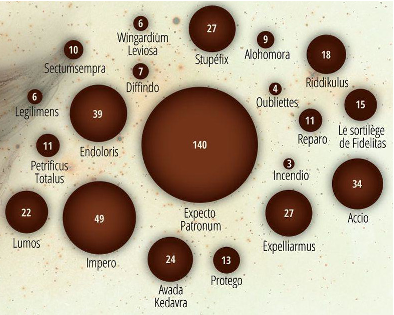
\includegraphics[width=8cm]{infographie}
   \end{center}
   {\footnotesize\it Source de l'infographie : Harry Potter, les nombres d'or de la saga, Le Figaro.fr, 2017}
   \begin{enumerate}
      \item Comment sont représentées les données dans cette infographie ?
      \item Combien y a-t-il eu de sortilèges donnés au total dans les sept livres ?
      \item Représenter les données dans un tableau en notant uniquement les sortilèges cités plus de 20 fois.
      \item Construire un diagramme en bâtons pour les valeurs de ce tableau.
      \item Construire un diagramme circulaire pour les valeurs de ce tableau.
      \item Laquelle de ces trois représentations vous convient le mieux ? Pourquoi ?
   \end{enumerate}
\end{exercice}

\begin{corrige}
   \ \\ [-5mm]
   \begin{enumerate}
      \item Les données sont représentées sous forme de {\blue bulles proportionnelles à l'effectif}.
      \item $140+49+39+34+27+27+24+22+18+15+13+11+11+10+9+7+6+6+4+3 =475$. \\
      {\blue 475 sorts ont été donnés durant les sept livres}.
      \item Tableau des effectifs : \\ \smallskip
         {\small
         \hautab{1}
         \setlength{\tabcolsep}{0cm}
         \begin{Ltableau}{\linewidth}{9}{c}
            \hline       
            Nom & E.P. & Imp. & End. & Accio &Stup. & Exp. & A.K. & Lum. \\
            \hline
            Eff. & 140 & 49 & 39 & 34 & 27 & 27 & 24 & 22 \\
            \hline
         \end{Ltableau}}
      \item Diagramme en bâtons : \\
         {\psset{yunit=0.4,xunit=0.8}
         \begin{pspicture}(-0.8,-1)(8,8.25)
         {\footnotesize
            \psline(0,0)(8,0)
            \multido{\i=0+1,\n=0+20}{8}{\psline(-0.1,\i)(0.1,\i) \rput(-0.5,\i){\n}}
            \psline{->}(0,0)(0,8)
            \psset{linewidth=0.5,linecolor=blue}
            \psline(0.5,0)(0.5,7)
            \psline(1.5,0)(1.5,2.45)
            \psline(2.5,0)(2.5,1.95)
            \psline(3.5,0)(3.5,1.7)
            \psline(4.5,0)(4.5,1.35)
            \psline(5.5,0)(5.5,1.35)
            \psline(6.5,0)(6.5,0.6)
            \psline(7.5,0)(7.5,0.55)
            \rput(0.5,-0.5){E.P.}
            \rput(1.5,-0.6){Imp.}
            \rput(2.5,-0.5){End.}
            \rput(3.5,-0.5){Accio}
            \rput(4.5,-0.6){Stup.}
            \rput(5.5,-0.6){Exp.}
            \rput(6.5,-0.5){A.K.}
            \rput(7.5,-0.5){Lum.}
            \rput(1,7.7){\it Effectifs}}
         \end{pspicture}}
      \item Diagramme circulaire : \\
         {\psset{unit=0.6}
         \footnotesize
         \begin{pspicture}(-5,-3.25)(3,3.25)
            \pscircle(0,0){3}
            \pswedge[fillstyle=solid,fillcolor=blue!70](0,0){3}{0}{139}
            \pswedge[fillstyle=solid,fillcolor=blue!65](0,0){3}{139}{188}
            \pswedge[fillstyle=solid,fillcolor=blue!60](0,0){3}{188}{227}      
            \pswedge[fillstyle=solid,fillcolor=blue!55](0,0){3}{227}{261}
            \pswedge[fillstyle=solid,fillcolor=blue!50](0,0){3}{261}{287}
            \pswedge[fillstyle=solid,fillcolor=blue!45](0,0){3}{287}{314}
            \pswedge[fillstyle=solid,fillcolor=blue!40](0,0){3}{314}{338}
            \pswedge[fillstyle=solid,fillcolor=blue!35](0,0){3}{338}{360}
            \rput(1.5;69){\white Expecto}
            \rput(2;69){\white Patronum}
            \rput{-17}(2;163){\white Impero}
            \rput{28}(2;208){\white Endoloris}
            \rput{62}(2.2;242){\white Accio}
            \rput{274}(2.2;274){\white Stupéfix}
            \rput{300}(1.9;300){\white Expelliarmus}
            \rput{326}(2.2;326){\white A.K.}
            \rput{349}(2.2;349){\white Lumos}
         \end{pspicture}}
      \item Cette question est personnelle\dots
   \end{enumerate}
\end{corrige}

\bigskip


\begin{exercice} %3
   Le tableau ci-dessous représente la répartition des médailles françaises aux Jeux olympiques d'été de 1896 à 2016 pour les dix sports ayant eu le plus de médailles.
   \begin{enumerate}
      \item Compléter le tableau.
      \item Comment est établi le classement des sports aux Jeux olympiques.
      \item Construire trois diagrammes circulaires : celui du cyclisme, du tir et du canoë-kayak en fonction de la couleur de médaille obtenue. Les comparer.
   \end{enumerate}
   \begin{center}
      \small
         {\hautab{2.1}
         \begin{tabular}{|*{7}{c|}}
            \hline 
            Pl. & & Sport & \pscircle[fillstyle=solid,fillcolor=Gold](0,0.1){0.2} & \pscircle[fillstyle=solid,fillcolor=lightgray](0,0.1){0.2} & \pscircle[fillstyle=solid,fillcolor=brown](0,0.1){0.2} & T. \\
            \hline
            1 & 
\includegraphics[height=4mm]{S1} & & & \, 51 \, & \, 35 \, & \, {\bf 118} \, \\
            \hline 
            2 & 
\includegraphics[height=4mm]{S2} & & 41 & & 23 & {\bf 91} \\
            \hline
            3 & 
\includegraphics[height=4mm]{S3} & & 14 & 25 & & {\bf 68} \\
            \hline  
            4 & 
\includegraphics[height=4mm]{S4} & & 14 & 13 & 10 & \\
            \hline  
            5 & 
\includegraphics[height=4mm]{S5} & & 14 & 10 & & {\bf 49} \\
            \hline  
            6 & \includegraphics[height=4mm]{S6} & & 13 & & 17 & {\bf 41} \\
            \hline  
            7 & 
\includegraphics[height=4mm]{S7} & & & 14 & 10 & {\bf 33} \\
            \hline  
            8 & 
\includegraphics[height=4mm]{S8} & & 9 & & 3 & {\bf 15} \\
            \hline  
            9 & 
\includegraphics[height=4mm]{S9} & & 8 & 15 & & {\bf 43} \\
            \hline  
            10 & 
\includegraphics[height=4mm]{S10} & {\textcolor{white}{Canoé-kayak}} & 8 & 9 & 19 & \\
            \hline    
         \end{tabular}} \\ [2mm]
      \hfill {\footnotesize\it Source : France aux Jeux olympiques, Wikipedia, 2019}
   \end{center}
\end{exercice}

\begin{corrige}
   \ \\ [-5mm]
   \begin{enumerate}
      \item Voici le tableau complété : \\ \smallskip
         {\footnotesize
         \hautab{2}
         \begin{tabular}{|*{7}{c|}}
            \hline 
             & & Sport & \pscircle[fillstyle=solid,fillcolor=Gold](0,0.1){0.2} & \pscircle[fillstyle=solid,fillcolor=lightgray](0,0.1){0.2} & \pscircle[fillstyle=solid,fillcolor=brown](0,0.1){0.2} & T. \\
            \hline
            1 & 
\includegraphics[scale=0.3]{../../S06_Interpreter_representer_des_donnees/Images/S1} & {\blue Escrime} & \, {\blue 32} \, & \, 51 \, & \, 35 \, & \, {\bf 118} \, \\
            \hline 
            2 & 
\includegraphics[scale=0.3]{../../S06_Interpreter_representer_des_donnees/Images/S2} & {\blue Cyclisme} & 41 & {\blue 27} & 23 & {\bf 91} \\
            \hline
            3 & 
\includegraphics[scale=0.3]{../../S06_Interpreter_representer_des_donnees/Images/S3} & {\blue Athlétisme} & 14 & 25 & {\blue 29} & {\bf 68} \\
            \hline  
            4 & 
\includegraphics[scale=0.3]{../../S06_Interpreter_representer_des_donnees/Images/S4} & {\blue Équitation} & 14 & 13 & 10 & {\blue \bf 37} \\
            \hline  
            5 & 
\includegraphics[scale=0.3]{../../S06_Interpreter_representer_des_donnees/Images/S5} & {\blue Judo} & 14 & 10 & {\blue 25} & {\bf 49} \\
            \hline  
            6 & \includegraphics[scale=0.3]{../../S06_Interpreter_representer_des_donnees/Images/S6} & {\blue Voile} & 13 & {\blue 11} & 17 & {\bf 41} \\
            \hline  
            7 & 
\includegraphics[scale=0.3]{../../S06_Interpreter_representer_des_donnees/Images/S7} & {\blue Tir} & {\blue 9} & 14 & 10 & {\bf 33} \\
            \hline  
            8 & 
\includegraphics[scale=0.3]{../../S06_Interpreter_representer_des_donnees/Images/S8} & {\blue Haltérophilie} & 9 & {\blue 3} & 3 & {\bf 15} \\
            \hline  
            9 & 
\includegraphics[scale=0.3]{../../S06_Interpreter_representer_des_donnees/Images/S9} & {\blue Natation} & 8 & 15 & {\blue 20} & {\bf 43} \\
            \hline  
            10 & 
\includegraphics[scale=0.3]{../../S06_Interpreter_representer_des_donnees/Images/S10} & {\blue Canoé-kayak} & 8 & 9 & 19 & {\blue \bf 36} \\
            \hline    
         \end{tabular}} \medskip
      \item Le classement des sports est établi grâce au {\blue nombre de médailles d'or}, puis d'argent, puis de bronze.
      \item On récapitule dans un tableau les angles : \\ \smallskip
   \end{enumerate}
      \small
      {\hautab{1.5}
      \begin{Ltableau}{0.95\linewidth}{5}{c}
         \hline   
         Couleur & Or & Argent & Bronze & Total \\
         \hline   
         Cyclisme & 41 & 27 & 23 & 91 \\
         Angle & \textcolor{blue}{\udeg{162}} & \textcolor{blue}{\udeg{107}} & \textcolor{blue}{\udeg{91}} & \udeg{360} \\
         \hline
         Tir & 9 & 14 & 10 & 33 \\
         Angle & \textcolor{blue}{\udeg{98}} & \textcolor{blue}{\udeg{153}} & \textcolor{blue}{\udeg{109}} & \udeg{360} \\
         \hline
         Canoé-kayak & 8 & 9 & 19 & 36 \\
         Angle & \textcolor{blue}{\udeg{80}} & \textcolor{blue}{\udeg{90}} & \textcolor{blue}{\udeg{190}} & \udeg{360} \\
        \hline
      \end{Ltableau}}
      {\psset{unit=0.4}
      \begin{pspicture}(-2,-3.3)(3,3.8)
         \pscircle(0,0){3}
         \pswedge[fillstyle=solid,fillcolor=Gold](0,0){3}{0}{162}
         \pswedge[fillstyle=solid,fillcolor=lightgray](0,0){3}{162}{269}
         \pswedge[fillstyle=solid,fillcolor=brown](0,0){3}{269}{360}      
      \end{pspicture}
      \begin{pspicture}(-3.5,-3)(3,3.5)
         \pscircle(0,0){3}
         \pswedge[fillstyle=solid,fillcolor=Gold](0,0){3}{0}{98}
         \pswedge[fillstyle=solid,fillcolor=lightgray](0,0){3}{98}{251}
         \pswedge[fillstyle=solid,fillcolor=brown](0,0){3}{251}{360}      
      \end{pspicture}
      \begin{pspicture}(-3.5,-3)(2.5,3.5)
         \pscircle(0,0){3}
         \pswedge[fillstyle=solid,fillcolor=Gold](0,0){3}{0}{80}
         \pswedge[fillstyle=solid,fillcolor=lightgray](0,0){3}{80}{170}
         \pswedge[fillstyle=solid,fillcolor=brown](0,0){3}{170}{360}      
      \end{pspicture}} \\
      \quad {\blue Cyclisme \hfill Tir \hfill Canoé-kayak} \hspace*{4mm} \\ \medskip
      On remarque par exemple que chacun de ces sports à une couleur très dominante : l'or pour le cyclisme, l'argent pour le tir et le bronze pour le canoé-kayak.  
\end{corrige} 

\end{colonne*exercice}


%%%%%%%%%%%%%%%%%%%%%%%%%%%%%%%%%%%%
%%%%%%%%%%%%%%%%%%%%%%%%%%%%%%%%%%%%
\Recreation

\begin{enigme}[Le tableur]
   Un tableur est un logiciel d'édition et de présentation de tableaux. Il comporte des \textbf{feuilles de calcul} composées de multiples lignes et colonnes formant des \textbf{cellules}. Chaque cellule est repérée par son adresse : une lettre désignant la colonne et un numéro désignant la ligne. Par exemple, la cellule {\bf A1} fait référence à la colonne A ligne numéro 1. \medskip

\partie[écrire dans une cellule] 
   Ouvrir une nouvelle feuille de tableur, écrire les textes suivants et appuyer sur entrée. 
   $$\text{Dans la cellule A1 : }  \Cell{\texttt{1+2}} \qquad ; \qquad \text{ Dans la cellule A2 :} \Cell{\texttt{=1+2}}$$
   Quelle est la différence entre ces deux écritures ? Quelle est la différence d'interprétation du tableur ? \par
   \Lignespointilles{2} \medskip

\partie[utilisation du tableaur-grapheur]
   Le ministère de la culture a effectué une enquête sur les équipements utilisés le plus souvent pour se connecter à Internet en 2019, en fonction de l'âge des utilisateurs.
   \begin{center}
      \begin{Tableur}[Bandeau=false,Colonnes=7,LargeurUn=5.5,Largeur=4.8]
         & 12-17 ans & 18-24 ans & 25-39 ans	 & 40-59 ans & 60-69 ans & 70 ans + \\
         Smartphone & 78\,\% & 89\,\% & 79\,\% & 45\,\% & 24\,\% & 12\,\% \\
         Ordinateur & 16\,\% & 10\,\% & 15\,\% & 42\,\% & 45\,\% & 38\,\% \\
      \end{Tableur}
   \end{center}
   On souhaite représenter, sous différentes formes, les résultats de cette enquête.
   \begin{enumerate}
      \item Reproduire ce tableau dans un tableur. \\
         {\it Enregistre ton travail dans un fichier nommé \texttt{Nom\_prenom\_classe\_tableur\_grapheur}.}
      \item Sélectionner le tableau en entier (cellules A1 à G3) et insérer trois graphiques : un diagramme en barres verticales (titre : graphique 1), un diagramme en barres horizontales (graphique 2) et un diagramme circulaire (graphique 3).
      \item Laquelle de ces trois représentations vous parait-elle la plus lisible, pourquoi ? \Lignespointilles{2}
      \item Choisir deux autres représentations et les décrire brièvement. \par
         Graphique 4 : \Lignespointilles{3} \par
         Graphique 5 : \Lignespointilles{3} \par
      \item Créer un graphique 6 de votre choix représentant uniquement les données concernant les ordinateurs.
      \item Répondre aux questions suivantes :
         \begin{enumerate}
            \item Quelle tranche d'âge utilise le plus son smartphone pour aller sur Internet ? \pointilles
            \item Selon toi, pourquoi \og les jeunes \fg{} utilisent-ils plus un smartphone qu'un ordinateur pour aller sur Internet ? \par
               \Lignespointilles{3}
            \item Selon toi, pourquoi \og les seniors \fg{} utilisent-ils plus un ordinateur qu'un smartphone pour aller sur Internet ? \par
               \Lignespointilles{3}         
         \end{enumerate}
   \end{enumerate}
\end{enigme}


\themaM
\graphicspath{{../../S07_Horaires_et_durees/Images}}

\chapter{Horaires et durées}
\label{S07}


%%%%%%%%%%%%%%%%%%%%%%%%%%%%%%%%%%%%%%%%%%
\begin{autoeval}
   \small
   \begin{enumerate}
      \item Il effectue des calculs de durées et d'horaires.
      \item Il vérifie la cohérence des résultats du point de vue des unités pour les calculs de durées.
      \item Il effectue des conversions d'unités de durée.
   \end{enumerate}
\end{autoeval}

\begin{prerequis}
   \begin{itemize}
      \item[\com] Mener des calculs impliquant des grandeurs mesurables, exprimer les résultats dans des les unités adaptées.
      \item[\com] Exprimer et vérifier la cohérence des résultats du point de vue des unités.
   \end{itemize}
\end{prerequis}

\vfill


\begin{debat}[Débat : instruments anciens de mesure de temps et de durée]
   De tous temps on a voulu mesurer le {\bf temps} et la {\bf durée}, ci-dessous figurent quelques instruments utilisés dans des époques plus ou moins lointaines. \\
   \textcolor{B1}{\small
   \begin{tabular}{*{4}{C{3.5}}}
      
\includegraphics[width=2.8cm]{cadran}
      &
      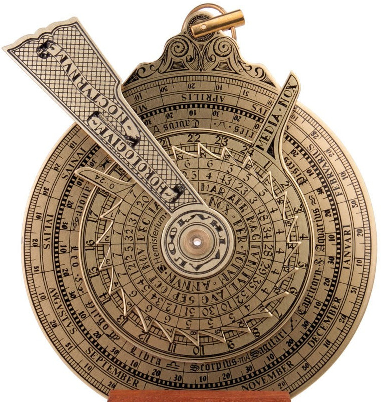
\includegraphics[width=2.8cm]{nocturlabe}
      &
      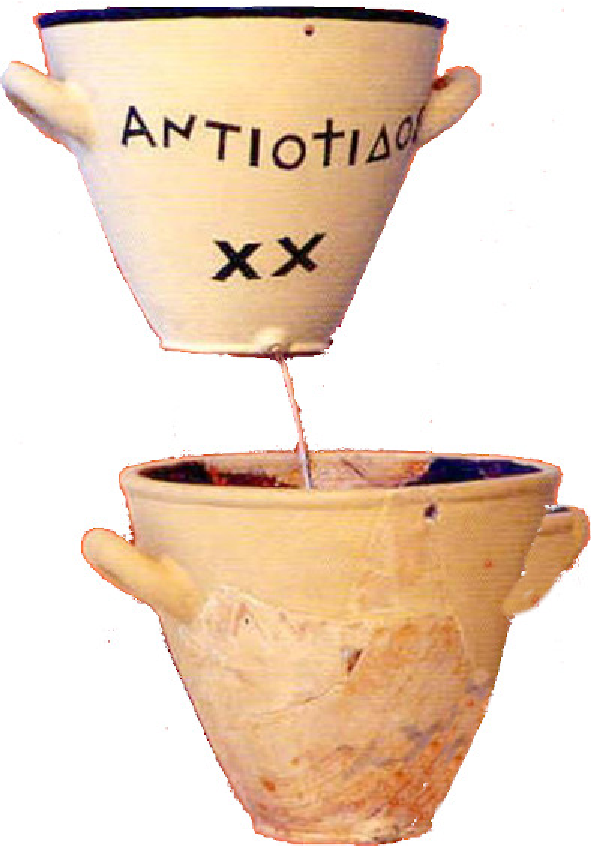
\includegraphics[width=2.8cm]{clepshydre}
      &
      
\includegraphics[width=2.8cm]{sablier} \\
      Cadran solaire & Nocturlabe & Clepsydre & Sablier \\
      1\,500 av. J.-C. & X\up{e} siècle & 1\,600 av. J.-C. & IX\up{e} siècle \\
      Heures du jour & Heures de la nuit & Durées longues (heures) & Durées courtes (minutes) \\
   \end{tabular}}
   \bigskip
   \begin{cadre}[B2][F4]
      \begin{center}
         Vidéo : \href{https://www.youtube.com/watch?v=8vMTE9U9z0U}{\bf Remettons les pendules à l'heure}, chaîne YouTube {\it C'est pas sorcier}.
      \end{center}
   \end{cadre}
\end{debat}


%%%%%%%%%%%%%%%%%%%%%%%%%%%%%%%
%%%%%%%%%%%%%%%%%%%%%%%%%%%%%%%
\activites
 
\begin{activite}[De la seconde au siècle]
   {\bf Objectif :} donner un ordre de grandeur dans le domaine des durées (plusieurs flèches peuvent arriver au même ordre de grandeur). \\
   \begin{QCM}
      Relier les durées suivantes à son ordre de grandeur.
      \begin{center}
         \begin{pspicture}(-8,-9)(8,9)
         {\psset{yunit=0.85}
            \rput(0,9){\cursive\large Le siècle}
            \rput(0,6){\cursive\large L'année}
            \rput(0,3){\cursive\large Le mois}
            \rput(0,0){\cursive\large Le jour}
            \rput(0,-3){\cursive\large L'heure}
            \rput(0,-6){\cursive\large La minute}
            \rput(0,-9){\cursive\large La seconde}
            \psdots(-1.5,-9)(-1.5,-6)(-1.5,-3)(-1.5,0)(-1.5,3)(-1.5,6)(-1.5,9)(1.5,-9)(1.5,-6)(1.5,-3)(1.5,0)(1.5,3)(1.5,6)(1.5,9)(-4,-10)(-4,-6)(-4,-2)(4,2)(4,6)(4,10)(4,-10)(4,-6)(4,-2)(-4,2)(-4,6)(-4,10)
            \rput(-6.25,-6){\parbox{3.5cm}{Temps mis par la lumière pour parcourir une distance équivalente à celle séparant la Terre et la Lune}}
            \rput(6.25,2){\parbox{3.5cm}{Durée d'un saison}}
            \rput(-6.25,2){\parbox{3.5cm}{Record du monde du \um{100}}}
            \rput(-6.25,-2){\parbox{3.5cm}{Temps de cuisson d'un \oe uf à la coque}}
            \rput(6.25,6){\parbox{3.5cm}{Intervalle entre deux battements de c\oe ur consécutifs}}
            \rput(-6.25,10){\parbox{3.5cm}{Durée d'un cycle complet de lune}}
            \rput(6.25,-6){\parbox{3.5cm}{Durée d'un film}}
            \rput(6.25,-10){\parbox{3.5cm}{Temps mis par la Terre pour faire le tour de son étoile : le Soleil}}
            \rput(6.25,10){\parbox{3.5cm}{Âge maximum atteint par un humain}}
            \rput(-6.25,6){\parbox{3.5cm}{Durée d'une grossesse}}
            \rput(6.25,-2){\parbox{3.5cm}{Durée d'un entraînement de sport}}
            \rput(-6.25,-10){\parbox{3.5cm}{Durée d'un weekend}}
            \multido{\n=-9+3}{7}{\rput(0,\n){\psframe(-1.2,-0.5)(1.2,0.5)}}}
         \end{pspicture}
      \end{center}
   \end{QCM}
\end{activite}


%%%%%%%%%%%%%%%%%%%%%%%%%%%%%%
%%%%%%%%%%%%%%%%%%%%%%%%%%%%%%
\cours 

 %%%%%%%%%%%%%
\section{Unités de temps}

Selon les situations, on indique les durées en années, mois, jours, heures, minutes, ou secondes : \\
1 siècle = 100 ans ; 1 an = 12 mois = 365/366 jours ; 1 jour = 24 heures ; 1 heure = 60 minutes = 3\,600 secondes\dots \\
Pour mesurer le temps ou une durée, on peut utiliser un cadran solaire, un sablier, une montre, un chronomètre\dots

%%%%%%%%%%%%%%%%
\section{Conversion de durées}

La seconde (s) est l'unité du système SI permettant de caractériser une durée. Contrairement aux autres unités, elle ne suit pas un système décimal, mais hexadécimal (de base 60).

\begin{methode*2*2}
   Pour convertir des heures en minutes ou des minutes en secondes ou inversement, on peut utiliser le schéma suivant : \\
   \begin{pspicture}(-1.5,-0.5)(11,3.3)
      \rnode{A}{\psframebox{durée en heures}}
      \hspace{12mm}
      \rnode{B}{\psframebox{durée en minutes}}
      \hspace{12mm}
      \rnode{C}{\psframebox{durée en secondes}}
      \nccurve[angle=90,linecolor=A1,offset=-1mm]{A}{B}
      \naput*{\textcolor{A1}{$\stackrel{\times60}{\longrightarrow}$}}
      \nbput*{\textcolor{A1}{$\stackrel{\div60}{\longleftarrow}$}}
      \nccurve[angle=90,linecolor=A1,offset=-1mm]{->}{B}{C}
      \naput*{\textcolor{A1}{$\stackrel{\times60}{\longrightarrow}$}}
      \nbput*{\textcolor{A1}{$\stackrel{\div60}{\longleftarrow}$}}
      \nccurve[angle=90,linecolor=B1]{->}{A}{C}
      \naput*{\textcolor{B1}{$\stackrel{\times3\,600}{\longrightarrow}$}}
      \nbput*{\textcolor{B1}{$\stackrel{\div3\,600}{\longleftarrow}$}}
   \end{pspicture}
   \exercice
      Convertir 170 minutes \par en heures et minutes.     
   \correction
      $170=2\times60+50$, donc \\
      $\umin{170} =\uh{2}\,\umin{50}$.
   \exercice
      Convertir \uh{1}\,\umin{25}\,\us{36} \par en secondes.
   \correction
      $\uh{1} =\us{3600}$ et $\umin{1} =\us{60}$ donc \\
      $\uh{1}\,\umin{25}\,\us{36} =\us{3600}+25\times\us{60}+\us{36} =\us{5136}$.
\end{methode*2*2}

\bigskip

Pour effectuer des additions ou soustractions de durées, on peut effectuer une opération en colonne (un peu périlleuse) ou procéder de proche en proche.
 
\begin{exemple}
\ \\ [-10mm]
  \begin{itemize}
      \item Un train part de Montpellier à \\
      8 h 48 min. La durée du trajet pour se rendre à Paris est de 3 h et 20 min. \\
      À quelle heure arrivera-t-il à Paris ?
      \item Un automobiliste part de Perpignan à 8 h 35 min et arrive à Montpellier à 10~h~20~min. Quelle est la durée de son trajet ?
   \end{itemize}
\correction
\ \\ [-8mm]
   \begin{itemize}
      \item   
      \begin{tabular}{ccccc}
         & 8 & h & 4 & 8 \\
         $+$ & 3 & h & 2 & 0 \\
         \hline
         1 & $\cancel{1}$ & h & $\cancel{6}$ & 8 \\
         \multicolumn{5}{c}{\psline{->}(0.5,0.3)(-0.5,-0.1)} \\
         1 & 2 & h & 0 & 8
      \end{tabular}
      \quad
      \begin{tabular}{p{5cm}}
        {\small on aligne les heures sous les heures, les minutes sous les minutes puis on additionne terme à terme. Si le nombre de minutes est supérieur à 60, on soustrait 60 min et on ajoute 1 h.} \\
      \end{tabular} 
      \medskip
      \item 8 h 35 $\xrightarrow{+\text{25 min}}$ 9 h 00 $\xrightarrow{+\text{1 h}}$ 10 h 00 $\xrightarrow{+\text{20 min}}$ 10 h 20. \\   
      La durée totale du trajet est de 1 h 45 min.
   \end{itemize}   
\end{exemple}

\medskip

\begin{remarque}
   attention à l'aspect hexadécimal de cette grandeur :
   \begin{itemize}
      \item lorsqu'on lit 1,5 h, cela correspond à 1 h et 0,5 h, c'est-à-dire 1h et 30 min ($0,5\times 60$ min).
      \item Inversement, 2 h 15 min ne correspond pas à 2,15 h mais à 2,25 h (15 min = $\frac{15}{60}$ h = 0,25 h).
   \end{itemize}
\end{remarque}


%%%%%%%%%%%%%%%%%%%%%%%%%%%%%%
%%%%%%%%%%%%%%%%%%%%%%%%%%%%%%
\exercicesbase

\begin{colonne*exercice}

\begin{exercice} %1
   Convertir les durées données ci-dessous en heures et minutes.
   \begin{enumerate}
      \item \uh{1,5}.
      \item \uh{2,25}.
      \item \uh{0,3}.
   \end{enumerate}
\end{exercice}

\begin{corrige}
   \ \\ [-5mm]
   \begin{enumerate}
      \item $\uh{1,5} =\blue \uh{1}\,\umin{30}$.
      \item $\uh{2,25} =\blue \uh{2}\,\umin{15}$.
      \item $\uh{0,3} =0,3\times\umin{60} =\blue \umin{18}$.
   \end{enumerate}
\end{corrige}

\bigskip


\begin{exercice} %2
   Convertir les durées données ci-dessous en heures décimales.
   \begin{enumerate}
      \item $\uh{6}\,\umin{30}$.
      \item $\uh{2}\,\umin{45}$.
      \item $\uh{8}\,\umin{33}$.
   \end{enumerate}
\end{exercice}

\begin{corrige}
   \ \\ [-5mm]
   \begin{enumerate}
      \item $\uh{6}\,\umin{30} =\blue \uh{6,5}$.
      \item $\uh{2}\,\umin{45} =\blue \uh{2,75}$. \smallskip
      \item $\uh{8}\,\umin{33} =\uh{8}+\frac{33}{60}\,\uh{} =\blue \uh{8,55}$.
   \end{enumerate}
\end{corrige}

\bigskip
 
 
\begin{exercice} %3
   Convertir les durées données ci-dessous en minutes.
   \begin{enumerate}
      \item \uh{1}\,\umin{56}.
      \item 2  j \umin{25}.
      \item 1 j \uh{20}\,\umin{3}.
   \end{enumerate}
\end{exercice}

\begin{corrige}
   \ \\ [-5mm]
   \begin{enumerate}
      \item $\uh{1}\,\umin{56} =1\times\umin{60}+\umin{56} =\blue \umin{116}$.
      \item $2\text{ j } \umin{25} =2\times24\times\umin{60}+\umin{25}$ \\
         \quad $=\umin{2880}+\umin{25} =\blue \umin{2905}$.
      \item $1\text{ j } \uh{20}\,\umin{3} =24\times\umin{60}+20\times\umin{60}+\small\umin{3}$ \\
         \quad $=\umin{1440}+\umin{1200}+\umin{3} =\blue \umin{2643}$.
   \end{enumerate}
\end{corrige}

\bigskip


\begin{exercice} %4
   Convertir les durées données ci-dessous en heures et minutes.
   \begin{enumerate}
      \item \umin{156}.
      \item \umin{296}.
      \item \umin{1603}.
   \end{enumerate}
\end{exercice}

\begin{corrige}
   \ \\ [-5mm]
   \begin{enumerate}
      \item $\umin{156} =2\times\umin{60}+\umin{36} =\blue \uh{2}\,\umin{36}$.
      \item $\umin{296} =4\times\umin{60}+\umin{56} =\blue \uh{4}\,\umin{56}$.
      \item $\umin{1603} =26\times\umin{60}+\umin{43}$ \\
         \quad $=\uh{26}\,\umin{43} =\blue 1\text{ j}\,\uh{2}\,\umin{43}$.
   \end{enumerate}
\end{corrige}

\bigskip


\begin{exercice} %5
   Effectuer les calculs suivants :
   \begin{enumerate}
      \item $\uh{3}\,\umin{45}+\uh{5}\,\umin{13}$
      \item $\uh{5}\,\umin{38}+\uh{9}\,\umin{43}$
      \item $\uh{11}\,\umin{28}-\uh{7}\,\umin{22}$
      \item $\uh{15}\,\umin{35}-\uh{9}\,\umin{49}$
   \end{enumerate}
\end{exercice}

\begin{corrige}
   \ \\ [-5mm]
   \begin{enumerate}
      \item $\uh{3}+\uh{5} =\uh{8}$ et $\umin{45}+\umin{13} =\umin{58}$ donc, $\uh{3}\,\umin{45}+\uh{5}\,\umin{13} =\blue \uh{8}\,\umin{58}$.
      \item $\uh{5}+\uh{9} =\uh{14}$ et \\
         $\umin{38}+\umin{43} =\umin{81} =\uh{1}+\umin{21}$ \\
         donc, $\uh{5}\,\umin{38}+\uh{9}\,\umin{43} =\blue \uh{15}\,\umin{21}$.
      \item $\uh{7}\,\umin{22} \quad \xrightarrow{+\umin{38}} \quad \uh{8}\,\umin{00}$ \\
         \quad\, $\uh{8}\,\umin{00} \quad \xrightarrow{+\uh{3}\;  \umin{28}} \quad \uh{11}\,\umin{28}$ \\
         $\uh{11}\,\umin{28}-\uh{7}\,\umin{22} =\uh{3}\,\umin{66} =\blue \uh{4}\,\umin{06}$.
      \item $\uh{9}\,\umin{49} \quad \xrightarrow{+\umin{11}} \quad \uh{10}\,\umin{00}$ \\
         \quad\, $\uh{10}\,\umin{00} \quad \xrightarrow{+\uh{5} \; \umin{35}} \quad \uh{15}\,\umin{35}$ \\   
         $\uh{15}\,\umin{35}-\uh{9}\,\umin{49} =\blue \uh{5}\,\umin{46}$.
   \end{enumerate}
\end{corrige}

\bigskip


\begin{exercice} %6
   Anita part à \uh{7}\,\umin{38} pour prendre le bus direction le collège Simone Veil. Elle met 6 minutes pour aller jusqu'à l'arrêt de bus, puis le trajet en bus dure 16 minutes et enfin il lui reste 4 minutes à pied. \\
   À quelle heure arrivera-t-elle au collège ?
\end{exercice}

\begin{corrige}
   Le temps de déplacement d'Anita est de \\
   $\umin{6}+\umin{16}+\umin{4} =\umin{26}$. \\
   Or, $\uh{7}\,\umin{38}+\umin{26} =\uh{7}\,\umin{64} =\uh{8}\,\umin{04}$. \\
   {\blue Anita devrait arriver au collège à \uh{8}\,\umin{04}}. \\
\end{corrige}

\bigskip


\begin{exercice} %7
   Douniya part du collège à pied à \uh{17}\,\umin{04}. Elle prévoit \umin{15}\,\us{30} pour le trajet, \umin{5} pour acheter un pain au chocolat et \umin{7} pour dire au revoir aux copines (et copains !). \\
   À quelle heure arrivera-t-elle chez elle ?
\end{exercice}

\begin{corrige}
   Le temps de déplacement de Douniya est de \\
   $\umin{15}\,\us{30}+\umin{5}+\umin{7} =\umin{27}\,\us{30}$. \\
   Or, $\uh{17}\,\umin{04}+\umin{27}\,\us{30} =\uh{17}\,\umin{31}\,\us{30}$. \\
   {\blue Douniya devrait arriver chez elle à \uh{17}\,\umin{31}\,\us{30}}. \\
\end{corrige}

\bigskip


\begin{exercice} %8
   Zayd part en promenade à \uh{9} 20. Il rentre à \uh{12}15, ne s'étant arrêté pour se reposer que lors de trois pauses de \umin{5} chacune. \\
   Pendant combien de temps a-t-il marché ?
\end{exercice}

\begin{corrige}
   $\uh{9}\,\umin{20} \quad \xrightarrow{+\umin{40}} \quad \uh{10}\,\umin{00}$ \\
   $\uh{10}\,\umin{00} \quad \xrightarrow{+\uh{2} \, \umin{15}} \quad \uh{12}\,\umin{15}$ \\
   La promenade de Zayd a duré \uh{2}\,\umin{55}. \\
   Or, il s'est arrêtée $3\times\umin{5} =\umin{15}$ donc, {\blue il a marché durant \uh{2}\,\umin{40}}. \\
\end{corrige}

\bigskip


\begin{exercice} %9
   Dans une usine, une machine met \umin{5}\,\us{26} pour fabriquer une pièce.
   \begin{enumerate}
      \item Combien de temps met-elle pour fabriquer 5 pièces ?
      \item Combien de temps met-elle pour en fabriquer 10 ?
      \item Combien de temps met-elle pour en fabriquer 20 ?
      \item Combien de temps met-elle pour en fabriquer 100 ?
      \item Combien la machine aura-t-elle fabriqué de pièces si elle fonctionne \uh{8} sans s’arrêter ?
      \item Une nouvelle machine, qui vient d’arriver à l’usine, met deux fois moins de temps pour fabriquer la même pièce. \\
      Quel temps met-elle pour fabriquer la pièce ?
   \end{enumerate}
\end{exercice}

\begin{corrige}
   \ \\ [-5mm]
   \begin{enumerate}
      \item $5\times\umin{5} =\umin{25} ; 5\times\us{26} =\us{130} =\umin{2}\,\us{10}$. \\
         $\umin{25}+\umin{2}\,\us{10} =\blue \umin{27}\,\us{10}$.
      \item $2\times(\umin{27}\,\us{10}) =\blue \umin{54}\,\us{20}$.
      \item $2\times(\umin{54}\,\us{20}) =\umin{108}\,\us{40} =\blue \uh{1}\,\umin{48}\,\us{40}$.
      \item $10\times(\umin{54}\,\us{20}) =\umin{540}\,\us{200} =\blue \uh{9}\,\umin{3}\,\us{20}$.
      \item $\uh{8} =8\times\us{3600} =\us{28800}$ et $\umin{5}\,\us{26} =5\times\us{60}+\us{26} =\us{326}$. \\
      Or, $28\,800\div326 \approx88,34$ donc, {\blue la machine aura fabriqué 88 pièces en \uh{8}}.
      \item La moitié de \umin{5} vaut \umin{2}\,\us{30} et la moitié de \us{26} vaut \us{13} donc, {\blue la machine met \umin{2}\,\us{43}}.
   \end{enumerate}
\end{corrige}

\bigskip


\begin{exercice} %10
   Résolution de problème : des robinets qui coulent. \\
   On dispose de deux robinets.
   \begin{itemize}
      \item Le premier est capable de remplir un réservoir d’eau de \ul{24} en 1 minute.
      \item Le second peut remplir ce même réservoir en 2 minutes.
   \end{itemize}
   En ouvrant les deux robinets au même moment, combien de temps faudrait-il pour remplir un jacuzzi avec \ul{1080} d’eau ? \\
   \begin{minipage}{4cm}
      \begin{enumerate}
         \item[a.] 15 min.
         \item[b.] 67,5 min.
         \item[c.] 135 min.
         \item[d.] 30 min.
      \end{enumerate}
   \end{minipage}
   \begin{minipage}{3cm}
      
\includegraphics[width=2.5cm]{robinet}
   \end{minipage}
   
   \qquad
   \begin{minipage}{2cm}
      \qrcode{https://www.youtube.com/watch?v=8vEacS_HnNw}
   \end{minipage}
   \qquad
   \begin{minipage}{4.2cm}
      {\it Un sketch sur la résolution de problème, par Gad Elmaleh}
   \end{minipage}
\end{exercice}

\begin{corrige}
   Pour un volume à remplir, le robinet R1 met deux fois moins de temps que le robinet R2. Donc, pendant le temps total, R1 remplit deux \og unités de volume \fg{} pendant que R2 n'en remplit qu’une : \\ [1mm]
   \ModeleBarre[Largeur=2.5cm]{PowderBlue 3 {"\ul{1080}"}}{DeepSkyBlue 1 "R1" DeepSkyBlue 1 "R1" LightSkyBlue 1 "R2"} \\
   En partageant le volume total en trois parties égales, on trouve $\ul{1080}\div3 =\ul{360}$.
   R2 remplit un tiers du volume total du jacuzzi : \ul{360}. \\
   Or, $360\div12 =30$. Sachant que R2 remplit \ul{12} en \umin{1}, il remplit \ul{360} en \ul{30}. \\
   {\blue La réponse est 30 minutes (d)}. \bigskip
\end{corrige}

\end{colonne*exercice}


%%%%%%%%%%%%%%%%%%%%%%%%
%%%%%%%%%%%%%%%%%%%%%%%%
\Recreation

\newcommand{\horloge}{\psset{fillstyle=none,linecolor=lightgray,linewidth=1.5mm}
      \multido{\n=0.0+2.8,\r=2.0+2.8}{4}{\psframe(0,\n)(11,\r)} %frames
      \multido{\n=2.75+2.75}{3}{\psline(\n,0)(\n,2)}
      \multido{\n=1+1}{10}{\psline(\n,2.8)(\n,4.8)}
      \multido{\n=2.75+2.75}{3}{\psline(\n,5.6)(\n,7.6)}
      \multido{\n=2.75+2.75}{3}{\psline(\n,8.4)(\n,10.4)}
      \pscircle(5.5,12.54){1.6}
      \multido{\n=2.4+2.8}{3}{\psarc(1.25,\n){0.4}{-90}{90}
         \psarc(4.25,\n){0.4}{90}{-90}
         \psline[linewidth=3mm](1.5,\n)(4,\n)
         \psarc(6.75,\n){0.4}{-90}{90}
         \psarc(9.75,\n){0.4}{90}{-90}
         \psline[linewidth=3mm](7,\n)(9.5,\n)}
      \psarc(4.75,10.75){0.35}{-90}{90}
      \psline[linewidth=2.5mm](5.1,10.75)(5.9,10.75)
      \psarc(6.25,10.75){0.35}{90}{-90}}


\begin{enigme}[Mengenlehreuhr]
   \partie[présentation]
      La {\bf Mengenlehreuhr} (en allemand \og Horloge de la théorie du jeu \fg) ou {\bf Berlin-Uhr} (\og Horloge de Berlin \fg) est la première horloge publique au monde qui indique l'heure au moyen de champs lumineux colorés, ce qui lui a valu d'entrer dans le livre Guinness des records lors de son installation le 17 juin 1975. \\
      {\it \small Source : \href{https://en.wikipedia.org/wiki/Mengenlehreuhr}{wikipedia}}

\medskip

   \partie[recherche]
      À partir des images suivantes représentant l'horloge à différents moments de la journée, déterminer le fonctionnement de l'horloge. Par groupe, vous construirez une affiche récapitulant vos recherches. \\
      \begin{center}
      {\psset{unit=0.54}
      \begin{minipage}{6cm}  
         \begin{pspicture}(0,-1.5)(11,13.8)
            \rput(5.5,6.5){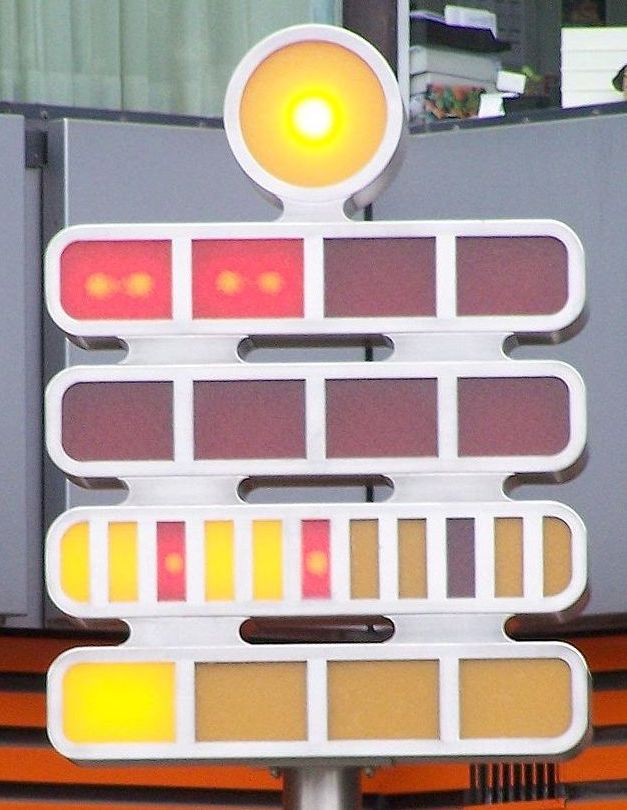
\includegraphics[width=6.7cm]{horloge_Berlin}}
         \end{pspicture}
      \end{minipage}
      \hspace{2cm}
      \begin{minipage}{6cm}  
         \begin{pspicture}(0,-1)(11,13.8)
            \psset{linecolor=yellow,fillstyle=solid,framearc=0.35}
               \psframe*(0,0)(2.75,2) %m1
               \psframe*(0,2.8)(5,4.8) %m5
               \pscircle*(5.5,12.54){1.6}
            \psset{linecolor=OrangeRed}
               \psframe*(2,2.8)(3,4.8) \psframe*(5,2.8)(6,4.8) %mi
               \psframe*(0,8.4)(5.5,10.4) %h5  
            \horloge
            \rput(5.5,-1){\large Il est 10h31}
         \end{pspicture}
      \end{minipage}
      
      \begin{minipage}{6cm}  
         \begin{pspicture}(0,-1)(11,15.5)

            \psset{linecolor=yellow,fillstyle=solid,framearc=0.35}
               \psframe*(0,0)(2.75,2) %m1
               \psframe*(0,2.8)(1,4.8) %m5
            \psset{linecolor=OrangeRed}
               \psframe*(0,5.6)(2.75,7.6) %h1
               \psframe*(0,8.4)(2.75,10.4) %h5  
            \horloge
            \rput(5.5,-1){\large Il est 6h06}
         \end{pspicture}
      \end{minipage}
      \hspace{2cm}
      \begin{minipage}{6cm}  
         \begin{pspicture}(0,-1)(11,15)
            \psset{linecolor=yellow,fillstyle=solid,framearc=0.35}
               \psframe*(0,2.8)(11,4.8) %m5
            \psset{linecolor=OrangeRed}
               \psframe*(2,2.8)(3,4.8) \psframe*(5,2.8)(6,4.8) \psframe*(8,2.8)(9,4.8) %mi
               \psframe*(0,5.6)(8.25,7.6) %h1
            \horloge
            \rput(5.5,-1){\large Il est 3h55}
         \end{pspicture}
      \end{minipage}}
      \end{center}
\end{enigme}

\begin{corrige}
   Chaque case allumée indique une durée écoulée :
   \begin{itemize}
      \item chaque case allumée de la première ligne en partant du haut représente 5 heures ;     
      \item chaque case allumée de la deuxième ligne représente 1 heure ;
      \item chaque case allumée de la troisième ligne représente 5 minutes. Les lumières rouges indiquent les quarts d’heure ;
      \item chaque case allumée de la dernière ligne représente 1 minute.
   \end{itemize}
  On additionne les durées pour obtenir l'heure.
\end{corrige}


%\themaN
\graphicspath{{../../S08_Expressions_litterales/Images/}}

\chapter{Expressions\\littérales}
\label{S08}


%%%%%%%%%%%%%%%%%%%%%%%%%%%%%%
%%%%%%%%%%%%%%%%%%%%%%%%%%%%%%
\begin{autoeval}
   \small
   \begin{enumerate}
      \item Il utilise les notations $2a$ pour $a\times2$ ou $2\times a$ et $ab$ pour $a\times b$, $a^2$ pour $a\times a$ et $a^3$ pour $a\times a\times a$.
      \item Il produit une expression littérale pour élaborer une formule ou traduire un programme de calcul.
      \item Il utilise une lettre pour traduire des propriétés générales.
      \item Il utilise une lettre pour démontrer une propriété générale.
   \end{enumerate}
\end{autoeval}

\begin{prerequis}
   \begin{itemize}
      \item Notion d'inconnue.
      \item[\com] Utiliser le calcul littéral pour traduire une propriété générale, pour démontrer un résultat général, pour valider ou réfuter une conjecture, pour modéliser une situation.
   \end{itemize}
\end{prerequis}

\vfill

\begin{debat}[Débat : petits contes mathématiques]
   Les vidéos des {\bf Petits contes mathématiques} ont été créés par {\it Universciences} : c'est une série pédagogique qui retrace l'histoire des maths à travers la découverte d'une notion, d'une formule, d'une conjecture ou d'une équation. Le récit est rythmé par des illustrations animées et la légèreté du ton dédramatise le sujet pour tous ceux qui ne seraient pas des \og matheux \fg. \\
   \begin{center}
      \begin{pspicture}(0,0)(5,3)
         \textcolor{B1}{
         \rput{10}(1,1){\huge $x$}
         \rput{20}(3.5,2.25){\huge $y$}
         \rput{-10}(3,0.5){\huge $z$}
         \rput(0.5,2.5){\huge $+$}
         \rput(2,1.5){\huge $\times$}
         \rput(4.5,2){\huge $()$}
         \rput(5,0.75){\huge $-$}
         \rput(2,3){\huge $\div$}
         \rput{-20}(5,3){\huge $t$}}
      \end{pspicture}
   \end{center}
   \bigskip
   \begin{cadre}[B2][J4]
      \begin{center}
         Vidéo : \href{https://leblob.fr/fondamental/le-x}{\bf Le $x$}, site Internet {\it Le blob}, épisode de la série {\it Petits contes mathématiques}.
      \end{center}
   \end{cadre}
\end{debat}


%%%%%%%%%%%%%%%%%%%%%%%%%%%%%%
%%%%%%%%%%%%%%%%%%%%%%%%%%%%%%
\activites

\begin{activite}[Des variables aux inconnues]
   {\bf Objectifs :} voir l'effet des variables dans un programme de calcul créé avec Scratch ; produire une expression littérale.
   \begin{QCM}
   On considère le programme de calcul ci-dessous dans lequel $x$, Etape 1, Etape 2 et Résultat sont quatre variables.
   \begin{center}
      \begin{Scratch}[Echelle=0.8]
         Place Drapeau ;
         Place Demander("Choisis un nombre");
         Place MettreVar("x",OvalCap("réponse"));
         Place DireT("Je multiplie le nombre par 6.","2");
         Place MettreVar("Etape 1",OpMul("6",OvalVar("x")));
         Place DireT("J'ajoute 10 au résultat.","2");
         Place MettreVar("Etape 2",OpAdd(OvalVar("Etape 1"),"10"));
         Place DireT("Je divise le résultat par 2.","2");
         Place MettreVar("Résultat",OpDiv(OvalVar("Etape 2"),"2"));
         Place Dire(OpRegrouper("J'obtiens finalement",OvalVar("Résultat")));
      \end{Scratch}
   \end{center}
   \begin{enumerate}
   {\psset{unit=0.9}
      \item Julien a fait fonctionner ce programme en choisissant le nombre 5.\\
      Vérifier que ce qui est dit à la fin est : \og J’obtiens finalement 20 \fg. Pour cela, remplir le diagramme suivant : \\
         \begin{pspicture}(-4,-0.2)(8,1.8)
            \psframe(0,0.5)(1,1.5)
            \rput(0.5,0){$x$}
            \psline[arrowsize=2mm]{->}(1.1,1)(2.4,1)
            \psframe(2.5,0.5)(3.5,1.5)
            \rput(3,0){étape 1}
            \psline[arrowsize=2mm]{->}(3.6,1)(4.9,1)
            \psframe(5,0.5)(6,1.5)
            \rput(5.5,0){étape 2}
            \psline[arrowsize=2mm]{->}(6.1,1)(7.4,1)
            \psframe(7.5,0.5)(8.5,1.5)
            \rput(8,0){résultat}
         \end{pspicture}         
      \item Que dit le programme si Zakariae le fait fonctionner en choisissant au départ le nombre 7 ? \\
          \begin{pspicture}(-4,-0.2)(8,1.8)
            \psframe(0,0.5)(1,1.5)
            \rput(0.5,0){$x$}
            \psline[arrowsize=2mm]{->}(1.1,1)(2.4,1)
            \psframe(2.5,0.5)(3.5,1.5)
            \rput(3,0){étape 1}
            \psline[arrowsize=2mm]{->}(3.6,1)(4.9,1)
            \psframe(5,0.5)(6,1.5)
            \rput(5.5,0){étape 2}
            \psline[arrowsize=2mm]{->}(6.1,1)(7.4,1)
            \psframe(7.5,0.5)(8.5,1.5)
            \rput(8,0){résultat}
         \end{pspicture}         
      \item Titouan fait fonctionner le programme, et ce qui est dit à la fin est : \og J’obtiens finalement 8 \fg. Quel nombre a-t-il choisi au départ ? \\
      \begin{pspicture}(-4,-0.2)(8,1.8)
            \psframe(0,0.5)(1,1.5)
            \rput(0.5,0){$x$}
            \psline[arrowsize=2mm]{<-}(1.1,1)(2.4,1)
            \psframe(2.5,0.5)(3.5,1.5)
            \rput(3,0){étape 1}
            \psline[arrowsize=2mm]{<-}(3.6,1)(4.9,1)
            \psframe(5,0.5)(6,1.5)
            \rput(5.5,0){étape 2}
            \psline[arrowsize=2mm]{<-}(6.1,1)(7.4,1)
            \psframe(7.5,0.5)(8.5,1.5)
            \rput(8,0){résultat}
         \end{pspicture} 
      \item Si l’on appelle $x$ le nombre choisi au départ, écrire en fonction de $x$ l’expression obtenue à la fin du programme. \par \medskip
         \pointilles}
   \end{enumerate}
   \end{QCM}
   \vfill\hfill{\footnotesize\it Cette activité est une adaptation du DNB 2017 de Pondichery.}
\end{activite} 


%%%%%%%%%%%%%%%%%%%%%%%%%%%%%
%%%%%%%%%%%%%%%%%%%%%%%%%%%%%
\cours 

\section{Expressions littérales} %%%%%

\medskip

\begin{definition}
   Une {\bf expression littérale} est une succession d'opérations où apparaissent des lettres représentant des nombres. On parle aussi d'{\bf expression algébrique}.
\end{definition}

\begin{exemple}
   $4\times x+3$ \; ; \; $2\times a-89$ \; ; \; $y-3\times z+t-4$.
\end{exemple}


%%%%%%%%%%%%%%%%%%%%%
\section{Produire une expression littérale}

On utilise notamment des expressions littérales pour produire des  formules générales, qui pourront être utilisées quelle que soit la valeur des variables.

\begin{exemple}[0.55]
\ \\ [-10mm]
   \begin{itemize}
      \item Matéo a quatre ans de plus que Noé. \\
         Exprimer l'âge de Matéo par rapport à celui de Noé.
      \item Un rectangle a pour largeur $\ell$ et pour longueur $L$. \\
         Donner l'expression de son aire et de son périmètre.
   \end{itemize}
   \correction
      \ \\ [-10mm]
      \begin{itemize}
         \item En appelant \og $\red x$ \fg{} l'âge de Noé, l'âge de Matéo peut s'écrire \og ${\red x}+4$ \fg.
         \item $\mathcal{A} =\ell\times L$. \\
         $\mathcal{P} =2\times(\ell+L)$.
      \end{itemize}
\end{exemple}

\medskip

\begin{remarque}
   la circonférence d'un disque s'écrit $2\pi R$ où :
   \begin{itemize}
      \item $\pi$ est une lettre grecque qui désigne le nombre 3,14\dots, qui est fixe ;
      \item $R$ est une lettre qui désigne le rayon du disque, ce nombre est variable et dépend du disque.
   \end{itemize}
\end{remarque}


%%%%%%%%%%%%%%%%%%%%%%%%%%%%%%%
\section{Simplifier d'une expression littérale}

Pour simplifier une expression littérale, on peut supprimer le signe \og $\times$ \fg{} devant une lettre, une parenthèse ou entre deux lettres. 

\begin{propriete}
   \begin{itemize}
      \item On utilise la notation $2a$ pour $a+a$ ou $a\times2$ ou encore $2\times a$. On dit \og deux a \fg.
      \item On utilise la notation $ab$ pour $a\times b$. On dit \og ab \fg.
      \item On utilise la notation $a^2$ pour $a\times a$. On dit \og a au carré \fg.
      \item On utilise la notation $a^3$ pour $a\times a\times a$. On dit \og a au cube \fg. \\ [-8mm]
   \end{itemize}
\end{propriete}

\bigskip

On écrit une expression comportant un nombre et une \og lettre \fg{} avec le nombre précédé de la \og lettre \fg.

\begin{exemple}[0.5]
   Simplifier les exepressions : \\
   $A =5\times y-2\times x$. \\
   $B =x\times x \times x + 7\times y\times y$. \\
   $C =x\times3$
   \correction
      $A =5y-2x$. \\
      $B =x^3+7y^2$. \\
      $C =3x$, est préférable à $C=x3$. Par commutativité de la multiplication, $x\times3 =3\times x =3x$.
\end{exemple}


%%%%%%%%%%%%%%%%%%%%%%%%%%%%%
%%%%%%%%%%%%%%%%%%%%%%%%%%%%%
\exercicesbase

\begin{colonne*exercice}

\begin{exercice} %1
   Si $x$ représente un nombre, comment peut-on écrire les expressions suivantes :
   \begin{enumerate}
      \item Le double de $x$.
      \item Le tiers de $x$.
      \item La somme de $x$ et de 13.
      \item La différence de $x$ et de 7.
      \item Le triple de la somme de 2 et de $x$.
      \item Le tiers de la différence de 16 et $x$.
   \end{enumerate}
\end{exercice}

\begin{corrige}
   \ \\ [-5mm]
   \begin{colenumerate}{2}
      \item $2\times x =\blue2x$ \smallskip
      \item $\dfrac13\times x =\blue\dfrac13x =\dfrac{x}{3}$ \smallskip
      \item $\blue x+13$
      \item $\blue x-7$
   \end{colenumerate}
   \begin{enumerate}
      \setcounter{enumi}{4}
      \item $3\times(2+x) =\blue3(2+x)$ \smallskip
      \item $\dfrac13\times(16-x) =\blue\dfrac13(16-x) =\dfrac{16-x}{3}$
   \end{enumerate}
\end{corrige}

\bigskip


\begin{exercice} %2
   Si on note $z$ l'âge en années de Rose aujourd'hui, comment peut-on noter :
   \begin{enumerate}
      \item L'âge qu'elle aura dans deux ans ?
      \item Le triple de l'âge qu'elle avait il y a quatre ans ?
      \item La moitié de l'âge qu'elle aura dans cinq ans ?
      \item Son année de naissance si on est en 2022 ?
   \end{enumerate}
\end{exercice}

\begin{corrige}
   \ \\ [-5mm]
   \begin{colenumerate}{2}
      \item $\blue z+2$
      \item $\blue 3(z-4)$
      \item $\blue \dfrac12(z+5) =\dfrac{z+5}{2}$ \smallskip
      \item $\blue 2021-z$
   \end{colenumerate}
\end{corrige}

\bigskip


\begin{exercice} %3
   Sahya construit un carré $ABCD$ de \ucm{5} de côté.
   \begin{enumerate}
      \item Calculer le périmètre $\mathcal{P}_1$ et l'aire $\mathcal{A}_1$ de $ABCD$.
      \item On augmente ses côtés de $k$ cm. Exprimer, en fonction de $k$ :
      \begin{itemize}
         \item la longueur $L$ du nouveau côté ;
         \item le nouveau périmètre $\mathcal{P}_2$ de ce carré ;
         \item la nouvelle aire $\mathcal{A}_2$ de ce carré.
      \end{itemize}
      \item Grâce aux expressions trouvées en 2, donner le périmètre et l'aire si on augmente le côté de 2 cm.
   \end{enumerate}
   {\psset{unit=1.2}
   \begin{pspicture}(-2,-1)(3,3.5)
      \pstGeonode[PosAngle={-135,-45,45,135},PointSymbol=none](0,0){A}(2,0){B}(2,2){C}(0,2){D}
      \psframe(0,0)(2,2)
      \psframe(0,0)(0.2,0.2)
      \psframe(0,0)(3,3)
      \psline{<->}(0,-0.5)(2,-0.5)
      \rput(1,-0.75){\small \ucm{5}}
      \psline{<->}(2,-0.5)(3,-0.5)
      \rput(2.5,-0.75){\small k}
   \end{pspicture}}
\end{exercice}

\begin{corrige}
   \ \\ [-5mm]
   \begin{enumerate}
      \item $\mathcal{P}_1 =4\times\ucm{5} =\blue\ucm{20}$ ; $\mathcal{A}_1 =(\ucm{5})^2 =\blue\ucmq{25}$
      \item Les longueurs sont en \ucm{} et les aires en \ucmq{}.
      \begin{itemize}
         \item La longueur $L$ du nouveau côté est $\blue5+k$.
         \item Le nouveau périmètre vaut $\mathcal{P}_2 =\blue4(5+k)$
         \item La nouvelle aire vaut $\mathcal{A}_2 =\blue(5+k)^2$
      \end{itemize}
      \item $\mathcal{P}_2 =4(5+2) \, \ucm{} = 4\times7 \, \ucm{} =\blue\ucm{28}$ et \\
      \quad\, $\mathcal{A}_2 =((5+2)\,\ucm{})^2 =(\ucm{7})^2 =\blue\ucmq{49}$
   \end{enumerate}
\end{corrige}

\bigskip


\begin{exercice} %4
Recopier les expressions suivantes en supprimant les signes $\times$ s'ils ne sont pas nécessaires.
\begin{enumerate}
   \item $A =9\times n$
   \item $B =x\times3$
   \item $C =12\times(a-3)$
   \item $D =2\times a(2\times8)$
   \item $E =n\times x$
   \item $F =2\times\pi\times R$
\end{enumerate}
\end{exercice}

\begin{corrige}
   \ \\ [-5mm]
   \begin{enumerate}
      \item $A =9\times n =\blue9n$
      \item $B =x\times3 =\blue3x$
      \item $C =12\times(a-3) =\blue12(a-3)$
      \item $D =2\times a(2\times8) =2\times16a =\blue32a$
      \item $E =n\times x =\blue nx$
      \item $F =2\times\pi\times R =\blue2\pi R$
\end{enumerate}
\end{corrige}

\bigskip

\begin{exercice} %5
   Simplifier les expressions suivantes :
   \begin{enumerate}
      \item $A =a\times a$
      \item $B =b\times b\times b$
      \item $C =c\times c\times3$
      \item $D =9+d\times d\times d$
      \item $E =a\times a\times b\times3$
      \item $F =x\times x\times x-2\times y\times y$
      \item $G =(a+b)\times(a+b)$
      \item $H =(x+y)(x+y)(x+y)$
   \end{enumerate}
\end{exercice}

\begin{corrige}
   \ \\ [-5mm]
   \begin{enumerate}
      \item $A =a\times a =\blue a^2$
      \item $B =b\times b\times b =\blue b^3$
      \item $C =c\times c\times3 =\blue3c^2$
      \item $D =9+d\times d\times d =\blue9+d^3$
      \item $E =a\times a\times b\times3 =\blue3a^2b$
      \item $F =x\times x\times x-2\times y\times y =\blue x^3-2y^2$
      \item $G =(a+b)\times(a+b) =\blue(a+b)^2$
      \item $H =(x+y)(x+y)(x+y) =\blue(x+y)^3$ \medskip
   \end{enumerate}
\end{corrige}

\bigskip


\begin{exercice} %6
   Dire si chaque affirmation est vraie ou fausse.
   \begin{enumerate}
      \item $x\times x = 2x$
      \item $x+x = 2x$
      \item $x\times x = x^{2}$
      \item $x+x =x^{2}$
      \item $x+2 =2x$
      \item $x+2=x^{2}$
   \end{enumerate}
\end{exercice}

\begin{corrige}
\ \\ [-5mm]
   \begin{colenumerate}{2}
      \item $x\times x = 2x$ : {\blue faux}.
      \item $x+x = 2x$ : {\blue vrai}.
      \item $x\times x = x^{2}$ : {\blue vrai}.
      \item $x+x =x^{2}$ : {\blue faux}.
      \item $x+2 =2x$ : {\blue faux}.
      \item $x+2=x^{2}$ : {\blue faux}.
   \end{colenumerate}
\end{corrige}

\bigskip


\begin{exercice} %7
   Voici un programme :
   \begin{center}
      \ProgCalcul[Enonce,Largeur=4.5cm]{
         Choisis un nombre,
         Retire-lui 5,
         Multiplie le résultat par 3}
   \end{center}
   \begin{enumerate}
      \item Faire fonctionner le programme avec trois nombres de son choix supérieurs ou égaux à 5.
      \item Quel nombre faut-il choisir pour obtenir 6 ?
      \item Soit $x$ le nombre de départ, donner l'expression finale en fonction de $x$.
   \end{enumerate}
\end{exercice}

\begin{corrige}
   \ \\ [-5mm]
   \begin{enumerate}
      \item \ProgCalcul{10,-5 *3}. Avec 10, on obtient {\blue 15} \dots
      \item \ProgCalcul[Direct=false]{7,-5 *3}. On obtient 6 avec {\blue 7}.
      \item \ProgCalcul[SansCalcul]{x,-5 *3,x-5 3(x-5)}.
   \end{enumerate}
\end{corrige}

\bigskip


\begin{exercice} %8
   Résoudre les défis suivants.
   \begin{enumerate}
      \item
         \begin{enumerate}
            \item Choisir deux nombres consécutifs, calculer leur somme et comparer avec les résultats de la classe.
            \item Quelle conjecture peut-on émettre ?
         \end{enumerate}
      \item On choisit un entier $n$.
         \begin{enumerate}
            \item Comment s'écrit le nombre suivant $n$ ?
            \item Donner l'expression de la somme de deux nombres consécutifs en fonction de $n$.
            \item Démontrer la conjecture.
         \end{enumerate}
      \item Montrer que la somme de trois nombres consécutifs est multiple de 3.
   \end{enumerate}
\end{exercice}

\begin{corrige}
\ \\ [-5mm]
   \begin{enumerate}
      \item
         \begin{enumerate}
            \item {\blue $16+17 =33$}.
            \item On peut conjecturer que  {\blue la somme de deux nombres consécutifs est un nombre impair}.
         \end{enumerate}
      \setcounter{enumi}{1}
      \item
         \begin{enumerate}
            \item Le nombre suivant $n$ s'écrit {\blue $n+1$}.
            \item $(n)+(n+1) =n+n+1 ={\blue 2n+1}$.
            \item $2n+1$ est un nombre pair ($2n$) auquel on ajoute 1, c'est donc un nombre impair. \\
               {\blue La conjecture est vraie}.
         \end{enumerate}
      \setcounter{enumi}{2}
      \item Soit $n$ un nombre quelconque, le suivant s'écrit $n+1$ et celui d'après $n+2$. \\
         La somme de trois nombres consécutifs s'écrit alors : \\
         $(n)+(n+1)+(n+2) =n+n+1+n+2 =3n+3$. \\
         $3n+3$ est la somme de deux nombres multiples de 3, {\blue c'est donc un multiple de 3}.
   \end{enumerate}
\end{corrige}
   
\flushright{\footnotesize\it D'après Sésamath, le manuel de cycle 4. Magnard 2016}

\end{colonne*exercice}


%%%%%%%%%%%%%%%%%%%%%%%%%%%%%%%
%%%%%%%%%%%%%%%%%%%%%%%%%%%%%%%
\Recreation

\def\croix{\psframe(0,-1)(1,2) \psframe(-1,-0)(2,1)}
\def\carre{\psframe(0,0)(1,1)}

\begin{enigme}[Défis !!!]

\vfill

\parbox{1.75cm}{
\includegraphics[width=2cm]{defi} \\ [2mm] \textcolor{orange}{\bf\large \, Défi 1}}
\qquad
\parbox{14.45cm}{
   Rayan et Aya ont choisi un nombre (entier positif). \\
   Rayan le multiplie par 5 et ajoute 35. \\
   Aya le multiplie par 2 et ajoute 146. \\
   Ils trouvent le même nombre à la fin. \\
   Quel nombre ont-ils choisi ?}

\vfill

\parbox{1.75cm}{
\includegraphics[width=2cm]{defi} \\ [2mm] \textcolor{orange}{\bf\large \, Défi 2}}
\qquad
\parbox{14cm}{
   Avec des petits carrés tous identiques, on construit un pattern selon le modèle évolutif ci-dessous : \\
   {\psset{unit=0.8}
   \begin{pspicture}(-3.5,-4.5)(4,3.75)
      \croix
      \rput(0.5,-2){Rang 1}
   \end{pspicture}
   \begin{pspicture}(-5,-4.5)(5,3.75)
      \croix
      \rput(2,0){\carre}
      \rput(0,2){\carre}
      \rput(-2,0){\carre}
      \rput(0,-2){\carre}
      \rput(0.5,-3){Rang 2}
   \end{pspicture}
   
   \begin{pspicture}(-8,-4.5)(4,1)
      \croix
      \rput(2,0){\carre}
      \rput(3,0){\carre}
      \rput(0,2){\carre}
      \rput(0,3){\carre}
      \rput(-2,0){\carre}
      \rput(-3,0){\carre}
      \rput(0,-2){\carre}
      \rput(0,-3){\carre}
      \rput(0.5,-4){Rang 3}
   \end{pspicture}}
   \begin{enumerate}
      \item Dessiner l’élément du rang suivant et expliquer la règle.
      \item Déterminer le nombre de petits carrés des éléments du rang 5, du rang 10, du rang 17.
      \item Déterminer le nombre de petits carrés de l’élément du rang 100 et donner un moyen de calculer rapidement le nombre de petits carrés d’un élément à n’importe quel rang.
     \item Existe-t-il un élément qui contient 532 petits carrés ? Un élément qui contient 813 petits carrés ?
  \end{enumerate}}
   
   \vfill\hfill {\it\small Source : La résolution de problèmes mathématiques au collège, MENJS, 2021}
 \end{enigme}  
 
\begin{corrige}
\hspace*{-7.5mm} \textcolor{orange}{\bf Défi 1} \\
   On peut modéliser ce défi par un schéma en barres. Soit $x$, le nombre choisi. \\
   \ModeleBarre[Separation=2]{DeepSkyBlue 1 "$x$" 1 "$x$" 1 "$x$" 1 "$x$" 1 "$x$" PowderBlue 2 "35"}{DeepSkyBlue 1 "$x$" 1 "$x$" SkyBlue 5 "146"}
   \ModeleBarre[Separation=3]{DeepSkyBlue 1 "$x$" 1 "$x$" 1 "$x$" PowderBlue 2 "35"}{ SkyBlue 3 "111" PowderBlue 2 "35"}
   \ModeleBarre{DeepSkyBlue 1 "$x$" 1 "$x$" 1 "$x$"}{SkyBlue 3 "111"} donc, $x =111\div3 ={\blue 37}$.

\hspace*{-7.5mm} \textcolor{orange}{\bf Défi 2} \\
   \begin{enumerate}
      \item Pour le rang 4, il suffit {\blue d'ajouter 1 carré à chacune des extrémités}.
      \item Au rang 1, on a 5 carrés. Au rang 2, $5+4 =9$ carrés. Au rang 3, $9+4 =13$ carrés.  Au rang 4, $13+4 =17$ carrés. {\blue Au rang 5, $17+4 =21$ carrés}. \\
         En continuant ainsi, on aura {\blue 41 carrés au rang 10 et 69 carrés au rang 17}.
         \item Soit $n$ le rang demandé, {\blue le nombre de carrés au rang $n$ est de $1+4\times n$}. \\
            Au rang 100, cela fait donc $1+4\times100 =401$.
         \item En enlevant 1 carré, on doit obtenir un multiple de 4. Or, $532-1 =531$ n'est pas un multiple de 4. \\
            $813-1 =812 =4\times203$ est un multiple de 4. \\
            {\blue Il y a donc 813 carrés au rang 203}.     
   \end{enumerate}
\end{corrige}


%\themaG
\graphicspath{{../../S09_Somme_des_angles_d_un_triangle/Images/}}

\chapter{Somme des angles\\d'un triangle}
\label{S09}

%%%%%%%%%%%%%%%%%%%%%%%%%%%%%%%%%%%%%%%%%
%%%%%%%%%%%%%%%%%%%%%%%%%%%%%%%%%%%%%%%%%
\begin{prerequis}
   \begin{itemize}
      \item Somme des angles d'un triangle.
   \end{itemize}
\end{prerequis}

\vfill

\begin{debat}[Débat : géométrie euclidienne VS géométrie sphérique]
   \og Un ours part de sa caverne et parcourt 10 km vers le sud, puis 10 km vers l'est et enfin 10 km vers le nord. Il se retrouve alors juste devant l'entrée de sa caverne. Quelle est la couleur de l'ours ? \fg \\ [2mm]
   La {\bf géométrie sphérique} n'a pas les même propriétés que la {\bf géométrie euclidienne} utilisée au collège et au lycée. Cette dernière est la géométrie initiée par {\it Euclide}, mathématicien grec né vers 330 av. J.-C., il est connu pour avoir recensé une grande partie des mathématiques de l'époque dans ses {\it Éléments} : une série de treize livres utilisée pendant près de 2\,000 ans qui fut l'ouvrage le plus édité au monde après la Bible. \\
   \begin{minipage}{4.5cm}
      \begin{pspicture}(0,0)(5,3.5)
         \pspolygon[linecolor=C1,linewidth=0.75mm](1,0.5)(4.5,0.5)(3,3.75)
      \end{pspicture}
   \end{minipage}
   \textcolor{B1}{
   \begin{minipage}{4cm}
      Un triangle \og plat \fg \\
      $\Longleftarrow$ \\ [5mm]
      \flushright Un triangle \og sphérique \fg \\
      \flushright $\Longrightarrow$
   \end{minipage}}
   \begin{minipage}{7cm}
      \psset{unit=0.8,lightsrc=10 0 10,viewpoint=50 -20 30,Decran=40,linecolor=gray!75} 
      \begin{pspicture}(-4,-4)(4,4)
         \psSolid[object=sphere,r=5,action=draw,ngrid=15 36]
         \psset{linecolor=C1,linewidth=1mm}
         \psarc(0,5.1){5.5}{-111}{-72}
         \psarc(3.5,-1.5){5.7}{128}{165.5}
         \psarc(-2.82,-0.47){4.47}{4}{51}
      \end{pspicture}
   \end{minipage} 
  \bigskip
   \begin{cadre}[B2][F4]
      \begin{center}
         Vidéo : \href{https://leblob.fr/videos/les-triangles-et-astronomie}{\bf Les triangles et l'astronomie}, site Internet {\it Le blob}, épisode de la série {\it Math.ing}.
      \end{center}
   \end{cadre}
\end{debat}

\vfill

\textcolor{PartieGeometrie}{\sffamily\bfseries Cahier de compétences} : chapitre 9, exercices 10 à 24.


%%%%%%%%%%%%%%%%%%%%%%%%%%%%%%%%%%
%%%%%%%%%%%%%%%%%%%%%%%%%%%%%%%%%%
\activites

\begin{activite}[Des angles mouvants]
   {\bf Objectif :} faire découvrir la propriété de la somme des angles d'un triangle.
   \begin{QCM}
   \partie[construction du triangle]
      \begin{enumerate}
         \item Sur une feuille, tracer un triangle ABC quelconque puis le découper.
         \item Colorier les trois angles de trois couleurs différentes des deux côtés du triangle (une couleur par angle). \\
         {\psset{unit=1.2}
         \begin{pspicture}(-2,0.2)(10,5.8)
            \rput(8.3,4.8){$\leftarrow$ colorier des deux côtés}
            \psline[linestyle=dashed](6,5)(6,1)(6.3,1)
            \psframe(6,1)(6.25,1.25)
            \pswedge[fillstyle=solid,fillcolor=B1,linecolor=B1](1,1){1}{0}{38.5}
            \pswedge[fillstyle=solid,fillcolor=A1,linecolor=A1](6,5){1}{218.8}{306.8}
            \pswedge[fillstyle=solid,fillcolor=J1,linecolor=J1](9,1){1}{127}{180}
            \pspolygon(1,1)(9,1)(6,5)
            \rput(0.7,1){B}
            \rput(9.3,1){C}
            \rput(6,5.3){A}
            \rput(6,0.7){H}     
         \end{pspicture}}
         \item Tracer la hauteur issue du sommet A et nommer le pied de cette hauteur H.
         \item Plier le triangle ABC de manière à placer le point A sur le point H.
         \item Plier le triangle ABC de manière à placer le point B sur le point H.
         \item Plier le triangle ABC de manière à placer le point C sur le point H.
      \end{enumerate}
   \partie[observations]
      \begin{enumerate}
         \item Que forment les trois angles obtenus en H ? \\ [5mm]
         \mbox{} \pfb \\
         \item Formuler cette observation en utilisant les angles $\widehat{\text A}, \widehat{\text B}$ et $\widehat{\text C}$. \\ [5mm]
         \mbox{} \pfb \\
         \item Formuler cette observation par une phrase simple et générale sans utiliser le nom des angles. \\ [5mm]
         \mbox{} \pfb \\ [5mm]
         \mbox{} \pfb \\
      \end{enumerate}
   \end{QCM}
\end{activite}

%%%%%%%%%%%%%%%%%%%%%%%%%%%%%%%%%%%%
%%%%%%%%%%%%%%%%%%%%%%%%%%%%%%%%%%%%
\cours 


%%%%%%%%%%%%%%%%%%%%%%%%%%%%%%%%%%%%
\section{Somme des angles dans un triangle}

\begin{propriete}
   Dans un triangle, la somme de la mesure de ses trois angles est égale à \udeg{180}.
\end{propriete}

\begin{center}
   \begin{pspicture}(-1,0.2)(9,5.5)
      \pswedge[fillstyle=solid,fillcolor=B1,linecolor=B1](1,1){1}{0}{38.5}
      \pswedge[fillstyle=solid,fillcolor=A1,linecolor=A1](6,5){1}{218.8}{306.8}
      \pswedge[fillstyle=solid,fillcolor=J1,linecolor=J1](9,1){1}{127}{180}
      \pspolygon(1,1)(9,1)(6,5)
      \rput(0.7,1){B}
      \rput(9.3,1){C}
      \rput(6,5.3){A} 
      \rput(5.5,2.5){$\widehat{A}+\widehat{B}+\widehat{C} =\udeg{180}$}
      \pswedge[fillstyle=solid,fillcolor=B1,linecolor=B1](0,3){1}{0}{38.5}
      \pswedge[fillstyle=solid,fillcolor=A1,linecolor=A1](0,3){1}{38.8}{126.8}
      \pswedge[fillstyle=solid,fillcolor=J1,linecolor=J1](0,3){1}{127}{180}
      \rput(-0.6,3.3){\white C}
      \rput(0.1,3.6){\white A}
      \rput(0.7,3.2){\white B}
   \end{pspicture}
\end{center}

\begin{exemple}
   \begin{pspicture}(-3,-0.8)(3,2)
      \psset{PointSymbol=none}
      \pstTriangle(2;15){A}(2;85){B}(2;195){C}
      \pstRightAngle[linecolor=A1]{C}{B}{A}
      \pstMarkAngle[linecolor=A1]{A}{C}{B}{?}
      \pstMarkAngle[linecolor=A1,MarkAngleType=double]{B}{A}{C}{\textcolor{A1}{\udeg{55}}} 
   \end{pspicture} \\
   Calculer la mesure de l'angle $\widehat{BCA}$.
   \correction
      D'après le codage, l'angle $\widehat{ABC}$ est droit, donc $\widehat{ABC} =\udeg{90}$. \\
      De plus, $\widehat{CAB} =\udeg{55}$.  \\
      Or, la somme des angles du triangle $ABC$ fait \udeg{180} d'où : \\
      $\widehat{CAB}+\widehat{ABC}+\widehat{BCA} =\udeg{180}$ \\
      $\udeg{55} +\udeg{90} +\widehat{BCA} =\udeg{180}$ \\
      $\widehat{BCA} =\udeg{180}-\udeg{55}-\udeg{90} =\udeg{35}$ 
\end{exemple}

\ \\ [2mm]

Par conséquent, pour qu'un triangle soit constructible, il est nécessaire que la somme de ses angles fasse \udeg{180}.


%%%%%%%%%%%%%%%%%%%%%%%%%%%%%%%%%%%%
\section{Triangles particuliers}

\begin{pspicture}(-1,-2)(4,3.5)
   \pstTriangle[PointSymbol=none](0,0){E}(4,0){C}(0,2){R}
   \psset{fillstyle=solid}
   \pstRightAngle[fillcolor=B1,linecolor=B1]{R}{E}{C}
   \pstMarkAngle[fillcolor=A1,linecolor=A1]{R}{C}{E}{}
   \pstMarkAngle[fillcolor=J1,linecolor=J1]{E}{R}{C}{}
   \rput(2,-1.5){\parbox{4cm}{\quad {\bf Triangle rectangle}\\ [3mm] la somme des deux angles aigus est égale à \udeg{90}}}
\end{pspicture}
\begin{pspicture}(-1.5,-3.5)(4,3.3)
   \pstTriangle[PointSymbol=none](0,1){I}(4,1){O}(2,3){S}
   \pstSegmentMark[SegmentSymbol=MarkHashh,MarkAngle=90]{I}{S} 
   \pstSegmentMark[SegmentSymbol=MarkHashh,MarkAngle=90]{S}{O}
   \pstLineAB{I}{O}
   \psset{linecolor=J1,fillstyle=solid,fillcolor=J1}
   \pstMarkAngle{S}{O}{I}{}
   \pstMarkAngle{O}{I}{S}{}
   \rput(2,-1.2){\parbox{4cm}{\qquad {\bf Triangle isocèle}\\ [3mm] les angles de la base ont la même mesure \\ [2mm] si le triangle est isocèle et rectangle, les angles de la base mesurent \udeg{45}}}
\end{pspicture}
\begin{pspicture}(-2,-2)(3,3.5)
   \pstTriangle[PointSymbol=none](0,0){E}(3,0){I}(1.5,2.55){Q}
   \psset{SegmentSymbol=MarkHash,MarkAngle=90}
   \pstSegmentMark{E}{Q} 
   \pstSegmentMark{I}{Q}
   \pstSegmentMark{I}{E}
   \psset{linecolor=J1,fillstyle=solid,fillcolor=J1,LabelSep=.75}
   \pstMarkAngle{Q}{I}{E}{\small \udeg{60}}
   \pstMarkAngle{I}{E}{Q}{\small \udeg{60}}
   \pstMarkAngle{E}{Q}{I}{\small \udeg{60}}
   \rput(1.5,-1.5){\parbox{3cm}{{\bf Triangle équilatéral}\\ [3mm] tous les angles\\mesurent \udeg{60}}}
\end{pspicture}


%%%%%%%%%%%%%%%%%%%%%%%%%%%%%%%%%%%%
%%%%%%%%%%%%%%%%%%%%%%%%%%%%%%%%%%%%
\exercicesbase

\begin{colonne*exercice}

\serie{Angles d'un triangle} %%%

\begin{exercice}%1
   Pour chaque cas, calculer la mesure de l'angle manquant dans le triangle $LEA$.
   \begin{center}
      {\hautab{1.25}
      \begin{ltableau}{0.8\linewidth}{3}
         \hline
         $\widehat{LEA}$ & $\widehat{EAL}$ & $\widehat{ALE}$ \\
         \hline
         \udeg{124} & \udeg{18} & \\
         \hline
         \udeg{71} & & \udeg{29} \\
         \hline
         & \udeg{98,1} & \udeg{59,6} \\
         \hline
         \udeg{49,5} & & \udeg{113} \\
         \hline
      \end{ltableau}}
   \end{center}
\end{exercice}

\begin{corrige}
   Pour chaque cas, la somme doit être égale à  \udeg{180}. \\ [1mm]
   {\hautab{1}
   \begin{ltableau}{0.9\linewidth}{3}
      \hline
      $\widehat{LEA}$ & $\widehat{EAL}$ & $\widehat{ALE}$ \\
      \hline
      \udeg{124} & \udeg{18} & \blue\udeg{38} \\
      \hline
      \udeg{71} & \blue\udeg{80} & \udeg{29} \\
      \hline
      \blue\udeg{22,3} & \udeg{98,1} & \udeg{59,6} \\
      \hline
      \udeg{49,5} & \blue\udeg{17,5} & \udeg{113} \\
      \hline
   \end{ltableau}}
\end{corrige}

\medskip

\begin{exercice}%2
   Les figures suivantes ne sont pas en vraie grandeur. Pour chacune d'elles, indiquer si elles sont constructibles ou non en justifiant la réponse. \\
   {\psset{unit=0.85}
   \small
   \begin{pspicture}(-0.5,0)(4,3.8)
      \pstTriangle[PointSymbol=none](0,0){A}(3,0){B}(2,3){C}
      \psset{LabelSep=.8}
      \pstMarkAngle{B}{A}{C}{\udeg{70}}
      \pstMarkAngle{C}{B}{A}{\udeg{75}} 
      \pstMarkAngle{A}{C}{B}{\udeg{40}} 
   \end{pspicture}
   \begin{pspicture}(-0.5,-0.5)(4,3)
      \pstTriangle[PointSymbol=none](0,2){F}(3.5,2){U}(2.2,0){O}
      \psset{LabelSep=.85}
      \pstMarkAngle{O}{F}{U}{\udeg{10}}
      \pstMarkAngle{U}{O}{F}{\udeg{95}} 
      \pstMarkAngle{F}{U}{O}{\udeg{85}} 
   \end{pspicture}   

   \begin{pspicture}(-1,-1)(4,3)
      \pstTriangle[PointSymbol=none](0,2){B}(0,0){O}(3,0){F}
      \pstMarkAngle{O}{B}{F}{\udeg{57,3}}
      \pstMarkAngle[LabelSep=1.2]{B}{F}{O}{\udeg{32,7}} 
      \pstRightAngle{F}{O}{B}
   \end{pspicture}
   \begin{pspicture}(-0.5,-1)(3.5,3.5)
      \pstTriangle[PointSymbol=none](1,0){P}(0,3){I}(3,2){C}
      \pstMarkAngle{P}{I}{C}{\udeg{35,1}}
      \pstMarkAngle[LabelSep=0.9]{C}{P}{I}{\udeg{72,4}}
      \psset{SegmentSymbol=MarkHashh,MarkAngle=90}
      \pstSegmentMark{P}{I}
      \pstSegmentMark{I}{C}
   \end{pspicture}}
\end{exercice}

\begin{corrige}
   \begin{itemize}
      \item $BAC$ : $\udeg{40}+\udeg{70}+\udeg{75} =\udeg{185} \neq \udeg{180}$. \\
         {\blue Le triangle $BAC$ n'est pas constructible}.
      \item $FOU$ : $\udeg{10}+\udeg{95}+\udeg{85} =\udeg{190} \neq \udeg{180}$. \\
         {\blue Le triangle $FOU$ n'est pas constructible}.
      \item $BOF$ : $\udeg{57,3}+\udeg{32,7}+\udeg{90} =\udeg{180}$. \\
         {\blue Le triangle $BOF$ est constructible}.
      \item $PIC$ : $\udeg{35,1}+\udeg{72,4}+\udeg{72,4} =\udeg{179,9} \neq \udeg{180}$. \\
         {\blue Le triangle $PIC$ n'est pas constructible}.
   \end{itemize}
\end{corrige}


\begin{exercice}%3
   Calculer, pour chaque triangle, la mesure de l'angle marqué d'un point d'interrogation. \\
   {\psset{unit=0.85}
   \small
   \begin{pspicture}(-1,0)(4,3.5)
      \pstTriangle[PointSymbol=none](0,0){R}(3,0){E}(1.5,2.6){P}
      \psset{SegmentSymbol=MarkHash,MarkAngle=90,LabelSep=0.8}
      \pstSegmentMark{R}{E}
      \pstSegmentMark{R}{P}
      \pstSegmentMark{P}{E}
      \pstMarkAngle{P}{E}{R}{?} 
   \end{pspicture}
   \begin{pspicture}(0,-0.5)(4,3)
      \pstTriangle[PointSymbol=none](0,2.3){R}(4,2.3){P}(2,0.3){A}
      \psset{SegmentSymbol=MarkHashh,MarkAngle=90}
      \pstSegmentMark{R}{A}
      \pstSegmentMark{P}{A}
      \pstMarkAngle[LabelSep=0.75]{P}{A}{R}{?} 
      \pstMarkAngle[LabelSep=0.9]{A}{R}{P}{\udeg{38}}
   \end{pspicture}
   
   \begin{pspicture}(-1,0.5)(4,3)
      \pstTriangle[PointSymbol=none](0,2){Y}(0,0){E}(3,0){S}
      \pstMarkAngle[LabelSep=1.1]{E}{Y}{S}{\small \udeg{50,36}}
      \pstRightAngle{S}{E}{Y}
      \pstMarkAngle[LabelSep=0.8]{Y}{S}{E}{?}
   \end{pspicture}
   \begin{pspicture}(-1,0.5)(3.5,3.5)
      \pstTriangle[PointSymbol=none](1,0){H}(0,3){W}(3,2){Y}
      \pstMarkAngle{H}{W}{Y}{\udeg{42,6}}
      \psset{SegmentSymbol=MarkHashh,MarkAngle=90}
      \pstSegmentMark{W}{H}
      \pstSegmentMark{W}{Y}
      \pstMarkAngle[LabelSep=0.8]{Y}{H}{W}{?}
   \end{pspicture}}
\end{exercice}

\begin{corrige}
      \begin{itemize}
      \item Le triangle $REP$ est équilatéral donc, tous ses angles ont la même mesure. La somme faisant \udeg{180}, un angle mesure $\udeg{180}\div3 =\udeg{60}$. \\
         Conclusion : {\blue $\widehat{REP} =\udeg{60}$}.
      \item Le triangle $RAP$ est isocèle en $A$ dont les angles à sa base principale mesurent \udeg{38}. \\
      $\udeg{38}+\udeg{38} =\udeg{76}$ d'où $\widehat{RAP} =\udeg{180}-\udeg{76} =\udeg{104}$. \\
      Conclusion : {\blue $\widehat{RAP} =\udeg{104}$}. 
      \item Le triangle $YES$ est rectangle en $E$ et $\udeg{90}+\udeg{50,36} =\udeg{140,36}$ d'où, $\widehat{ESY} =\udeg{180}-\udeg{140,36} =\udeg{39,64}$. \\
         Conclusion : {\blue $\widehat{ESY} =\udeg{39,64}$}. 
      \item Le triangle $WHY$ est isocèle en $W$ dont l'angle à son sommet principal vaut \udeg{42,6}. \\
         $\udeg{180}-\udeg{42,6} =\udeg{137,4}$ ; $\widehat{WHY} =\udeg{137,4}\div2 =\udeg{68,7}$. \\
         Conclusion : {\blue $\widehat{WHY} =\udeg{68,7}$}.
   \end{itemize}
\end{corrige}


\serie{Défis !}%%%%%%%%%%%%%%%%%%%%%%%

%\begin{exercice}%7
%   On considère la figure suivante : \\
%   \begin{pspicture}(-0.5,0)(8,5)
%      \pstGeonode[CurveType=polygon,PointSymbol=none,PosAngle={90,225,45,-45}](1.9,3.9){C}(0.5,1){E}(7,4){I}(5.2,0.9){A}
%      \pstGeonode[PointSymbol=none,PosAngle=90](3.55,2.4){L}
%      \pstSegmentMark{A}{I}
%      \pstSegmentMark{L}{I}
%      \pstMarkAngle{I}{E}{C}{\udeg{38}}
%      \pstMarkAngle{E}{I}{A}{\udeg{38}}
%   \end{pspicture}
%   \begin{enumerate}
%      \item Démontrer que les droites $(CE)$ et $(IA)$ sont parallèles.
%      \item Démontrer que les angles $\widehat{IAL}$ et $\widehat{ILA}$ ont la même mesure que l'on calculera.
%      \item Quelle est la nature du triangle $CLE$ ?
%   \end{enumerate}
%\end{exercice}
%
%\begin{corrige}
%  \ \\ [-5mm]
%   \begin{enumerate}
%      \item Les angles $\widehat{CEL}$ et $\widehat{LIA}$ sont alternes-internes et de même mesure, donc \\
%         {\blue les droites $(CE)$ et $(IA)$ sont parallèles}.      
%      \item Le triangle $ALI$ est isocèle en $I$, les angles à sa base principale sont donc égaux d'où : {\blue $\widehat{IAL} =\widehat{ILA}$}. \\
%         On calcule leur mesure :
%         $\udeg{180}-\udeg{38} =\udeg{142}$ et $\udeg{142}\div2 =\udeg{71}$. D'où {\blue $\widehat{IAL} =\widehat{ALI} =\udeg{71}$}.
%      \item Les angles $\widehat{ALI}$ et $\widehat{CLE}$ sont opposés par le sommet $L$ donc ils sont égaux, d'où $\widehat{CLE} =\udeg{71}$. \\
%         Le triangle $CLE$ a deux angles égaux au triangle $ALI$ donc, le troisième angle est également le même soit $\widehat{ACL} =\widehat{IAL} =\udeg{71}$. \\
%        Conclusion : {\blue le triangle $CLE$ est isocèle en $E$}.
%   \end{enumerate}
%\end{corrige}
%
%\bigskip

\begin{exercice}%4
   Dans la figure ci-dessous, les points $O, U, D$ et $A$ sont alignés. Des mesures d'angle sont indiquées. \\
   Le triangle $HOA$ est rectangle en $H$ ?
   \begin{center}
   {\psset{unit=0.7}
   \small
   \begin{pspicture}(-1.5,-0.5)(9.4,4)
      \psline[linestyle=dashed](4,0)(2,3.46)(0,0)
      \psline[linestyle=dashed](9.4,0)(2,3.46)(6.1,0)
      \psline(10,0)(-1,0)
      \rput(0,-0.3){$O$}
      \rput(4,-0.3){$U$}
      \rput(2,3.9){$H$}
      \rput(6.2,-0.3){$D$}
      \rput(9.5,-0.3){$A$}
      \psarc(0,0){0.5}{60}{180}
      \psarc(4,0){0.6}{120}{180}
      \psarc(6.1,0){0.7}{140}{180}
      \psarc(9.4,0){0.8}{155}{180}
      \rput(5.1,0.3){\udeg{40}}
      \rput(8,0.25){\udeg{25}}
      \rput(-0.6,0.8){\udeg{120}}
      \rput(3.1,0.4){\udeg{60}}
   \end{pspicture}}
   \end{center}
\end{exercice}

\begin{corrige}
   \begin{itemize}
      \item L'angle $\widehat{HOU}$ est supplémentaire à l'angle de mesure \udeg{120}, donc il mesure $\udeg{180}-\udeg{120} =\udeg{60}$.
      \item Dans le triangle $HOA$ : \\
         $\widehat{HOA}+\widehat{OAH} = \udeg{60}+\udeg{25} =\udeg{85}$ soit : \\
         $\widehat{OHA} =\udeg{180}-\udeg{85} =\udeg{95} \neq\udeg{90}$. \\
         Donc, {\blue le triangle $HOA$ n'est pas rectangle en $H$}.
   \end{itemize}
\end{corrige}


\begin{exercice}%5
   Sachant que les droites $(OS)$ et $(AC)$ sont parallèles, calculer la mesure de chacun des angles du quadrilatère $OSCA$ en justifiant. \\
   {\psset{unit=0.9}
   \small
   \begin{pspicture}(-3.5,-0.5)(5,4.4)
      \pstGeonode[CurveType=polygon,PointSymbol=none,PosAngle={90,-90,-45}](3,4){R}(0,0){A}(5,0){C}
      \pstGeonode[PointSymbol=none,PosAngle={0,180}](4,2){S}(1.48,2){O}
      \pstLineAB{O}{S}
      \pstMarkAngle[LabelSep=0.8]{O}{R}{S}{\udeg{64}}
      \psline(-2,0)(0,0)
      \rput(-1.8,0.3){$x$}
      \psarc(0,0){0.3}{53}{180}
      \rput(-0.2,0.6){\udeg{127}}
   \end{pspicture}}
\end{exercice}

\begin{corrige}
   \begin{itemize}
      \item L'angle $\widehat{CAO}$ est le supplémentaire de l'angle $\widehat{xAO}$ de mesure $\udeg{127}$, donc il mesure $\udeg{180}-\udeg{127} =\udeg{53}$. Soit : {\blue $\widehat{CAO} =\udeg{53}$}.
      \item Les angles $\widehat{xAO}$ et $\widehat{AOS}$ sont alternes-internes et les droites $(OS)$ et $(AC)$ sont parallèles donc, ces deux angles sont égaux. Soit {\blue $\widehat{AOS} =\udeg{127}$}.
      \item Les angles $\widehat{CAO}$ et $\widehat{SOR}$ sont correspondants et les droites $(OS)$ et $(AC)$ sont parallèles, ils sont donc égaux et $\widehat{SOR} =\udeg{53}$. \\
         Dans le triangle $ROS, \widehat{SOR}+\widehat{ORS}+\widehat{RSO} =\udeg{180}$. \\ 
         Donc, $\udeg{53}+\udeg{64}+\widehat{RSO} =\udeg{180}$ soit $\widehat{RSO} =\udeg{180}-\udeg{53}-\udeg{64} =\udeg{63}$. \\
          Les angles $\widehat{RSO}$ et $\widehat{OSC}$ sont supplémentaires donc, $\widehat{OSC} =\udeg{180}-\udeg{63} =\udeg{117}$. {\blue $\widehat{OSC} =\udeg{117}$}.
      \item Les angles $\widehat{RSO}$ et $\widehat{SCA}$ sont correspondants et les droites $(OS)$ et $(AC)$ sont parallèles donc, ces deux angles sont égaux. Soit : {\blue $\widehat{SCA} =\udeg{63}$}.
   \end{itemize}
\end{corrige}


\begin{exercice}%6
   On considère la figure suivante : \\
   {\psset{unit=0.8}
   \small
   \begin{pspicture}(-3,-0.5)(8,8.2)
      \pstGeonode[PointSymbol=none,PosAngle={-135,-45,45,135,90,90}](0,0){A}(4,0){S}(4,4){H}(0,4){R}(0.54,2){U}(2,7.46){T}
      \psset{SegmentSymbol=MarkHashh,MarkAngle=90}
      \pstSegmentMark{A}{R}
      \pstSegmentMark{S}{A}
      \pstSegmentMark{S}{H}
      \pstSegmentMark{S}{U}
      \pstSegmentMark{U}{H}
      \pstSegmentMark{R}{H}
      \pstSegmentMark{T}{R}
      \pstSegmentMark{T}{H}
      \pstRightAngle{R}{A}{S}
   \end{pspicture}}
   \begin{enumerate}
      \item Quelle est la nature des triangles $ASU$ et $UHT$ ?
      \item 
      \begin{itemize}
         \item Calculer l'angle $\widehat{ASU}$.
         \item Calculer l'angle $\widehat{UHT}$.
      \end{itemize}
      \item Calculer alors la mesure des angles $\widehat{SAU}$ et $\widehat{HUT}$.
      \item Que peut-on dire des points $A, U$ et $T$ ? Justifier.
   \end{enumerate}
\end{exercice}

\begin{corrige}
   \ \\ [-5mm]
   \begin{enumerate}
      \item $AS =SU$ donc, {\blue le triangle $ASU$ est isocèle en $S$}. \\
      $UH = HT$ donc, {\blue le triangle $UHT$ est isocèle en $H$}.
      \item
      \begin{enumerate}
         \item Le triangle $SUH$ est équilatéral, la mesure de ses angles est donc de \udeg{60}. \\
          Le quadrilatère $RHSA$ possède quatre côtés égaux et un angle droit, c'est donc un carré. \\
         On a alors ${\blue \widehat{ASU}} =\widehat{ASH}-\widehat{USH} =\udeg{90}-\udeg{60} ={\blue \udeg{30}}$. \\
         \item le triangle $THR$ est équilatéral, la mesure de ses angles est donc de \udeg{60}. \\ 
         De plus, $\widehat{UHR} =\widehat{SHR}-\widehat{SHU} =\udeg{90}-\udeg{60} =\udeg{30}$. \\
         Soit ${\blue \widehat{UHT}} =\widehat{UHR} +\widehat{RHT} =\udeg{30}+\udeg{60} ={\blue \udeg{90}}$. \\
      \end{enumerate}
      \setcounter{enumi}{2}
      \item \textcolor{G1}{$\bullet$} Dans le triangle $ASU$ isocèle en $S$, $\widehat{ASU} =\udeg{30}$ donc, la somme des deux angles restants vaut $\udeg{180}-\udeg{30} =\udeg{150}$ et comme ils sont égaux, ils valent chacun $\udeg{150}\div2 =\udeg{75}$. \\
      Soit : {\blue $\widehat{SAU} =\widehat{SUA} =\udeg{75}$}. \\
          \textcolor{G1}{$\bullet$} Dans le triangle $UHT$ isocèle en $H$, $\widehat{UHT} =\udeg{90}$ donc, la somme des deux angles restants vaut $\udeg{180}-\udeg{90} =\udeg{90}$ et comme ils sont égaux, ils valent chacun $\udeg{90}\div2 =\udeg{45}$. \\
          Soit : {\blue $\widehat{HUT} = \widehat{HTU} =\udeg{45}$}.
      \item $\widehat{AUT} =\widehat{AUS}+\widehat{SUH}+\widehat{HUT}$. \\
      \quad\, $\widehat{AUT} =\udeg{75}+\udeg{60}+\udeg{45} =\udeg{180}$. \\
      Conclusion : {\blue les points $A, U$ et $T$ sont alignés}.
   \end{enumerate}
\end{corrige}

\end{colonne*exercice}


%%%%%%%%%%%%%%%%%%%%%%%%%%%%%%%%%%%
%%%%%%%%%%%%%%%%%%%%%%%%%%%%%%%%%%%
\Recreation

\enigme[Le triangle de Penrose]{

\partie[le triangle de Penrose, kesako ?]

Le {\it triangle de Penrose}, aussi appelé tripoutre ou tribarre est un triangle impossible à construire physiquement en 3D mais facilement modélisable en 2D. Il a été conçu par le physicien et mathématicien britanique {\bf Roger Penrose} (né à Colchester en 1931) dans les années 1950.
\begin{enumerate}
   \item Observer le triangle de Penrose et en particulier ses angles sur ce quadrillage à maille triangulaire (aussi appelé isométrique en raison de l'égalité de longueur de tous ses côtés). Pourquoi est-il impossible à construire ?
   \item Le reproduire sur le quadrillage juste à droite puis le colorier. \bigskip
\end{enumerate}
\begin{pspicture*}(0,2.5)(18,10.5)
   \pstVerb{gsave [0.866 0.5 0 1 0 -400] concat }
   {\psset{linewidth=0.3pt,linecolor=black!40}
      \multido{\iA=-0+1,\iB=-10+1,\iC=-25+1}{40}{
         \psline(\iA,-4)(\iA,20)
         \psline(-5,\iB)(20,\iB)
         \rput(0,\iC){\psline(0,0)(!\iA\space abs dup add dup )}
      }
   }
   \pspolygon[fillstyle=solid,fillcolor=PartieStatistique](2,2)(1,2)(1,8)(6,8)(5,7)(2,7)
   \pspolygon[fillstyle=solid,fillcolor=PartieStatistique!25](2,2)(2,7)(3,7)(3,4)(8,9)(8,8)
   \pspolygon[fillstyle=solid,fillcolor=PartieStatistique!50](3,4)(3,5)(6,8)(1,8)(2,9)(8,9)
   \pstVerb{grestore }
\end{pspicture*} \smallskip

\partie[et dans la vraie vie ?]

$\Rightarrow$ Le jeu {\bf Monument Valley} est un jeu de réflexion en perspective isométrique qui se passe dans un décor composé de structures aux formes géométriques impossibles basées sur ce triangle. \\ [2mm]
$\Rightarrow$ {\bf An impossible triangle sculpture in Perth} : in 1997, a new landmark has been created for Perth, in a unique collaboration between a leading WA artist Brian McKay and architect Ahmad Abas. Destined to become a bold icon for Perth, the \og Impossible Triangle \fg{} has been erected in Claisebrook Square, East Perth. The sculpture is 13.5 meters height and the design striations on the polished aluminium reflects both sunlight and artificial lighting. The view of the triangle depends on where it is observed from. \hfill {\footnotesize\it Source : https://im-possible.info/english/}
\medskip

\begin{center}
   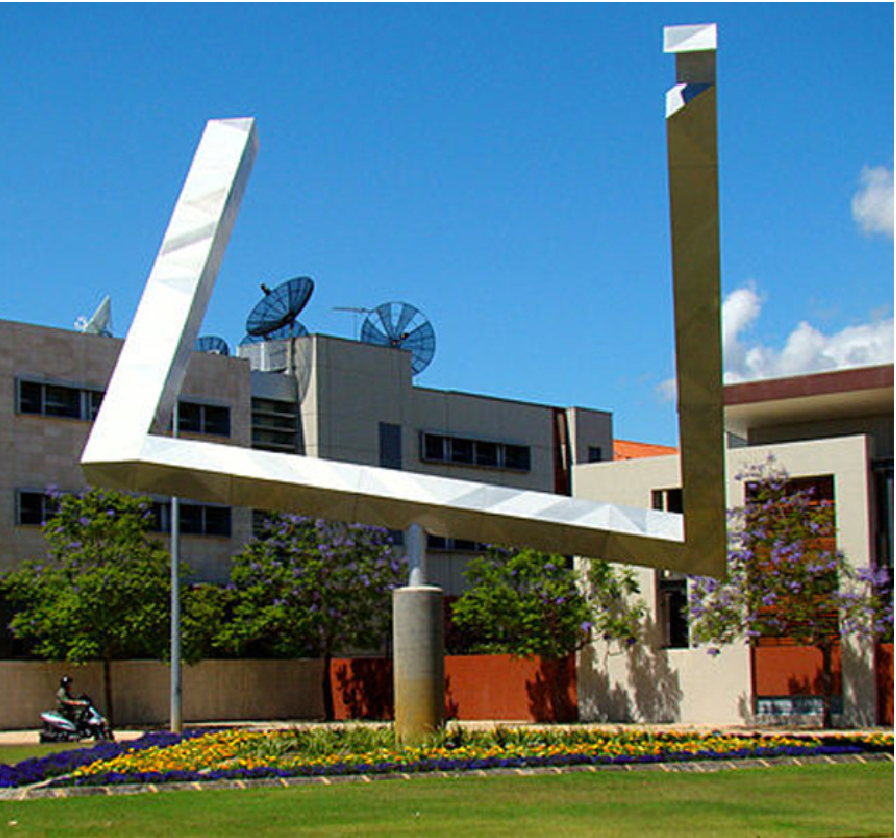
\includegraphics[height=3.5cm]{Penrose1} \qquad 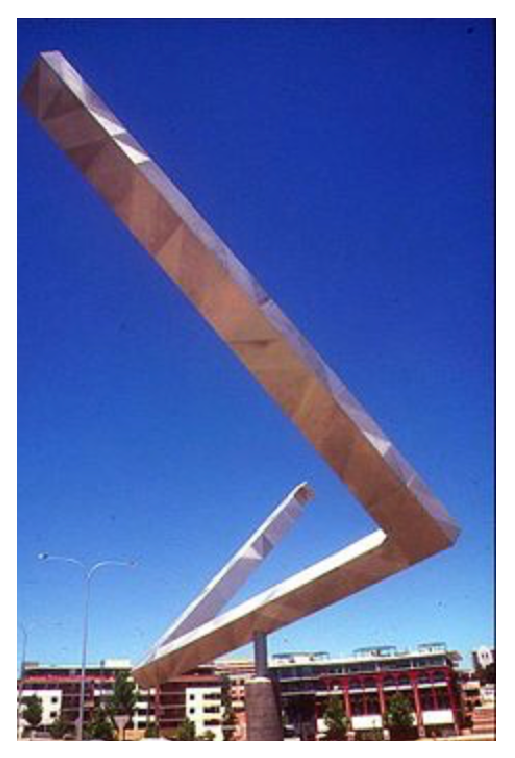
\includegraphics[height=3.5cm]{Penrose2} \qquad 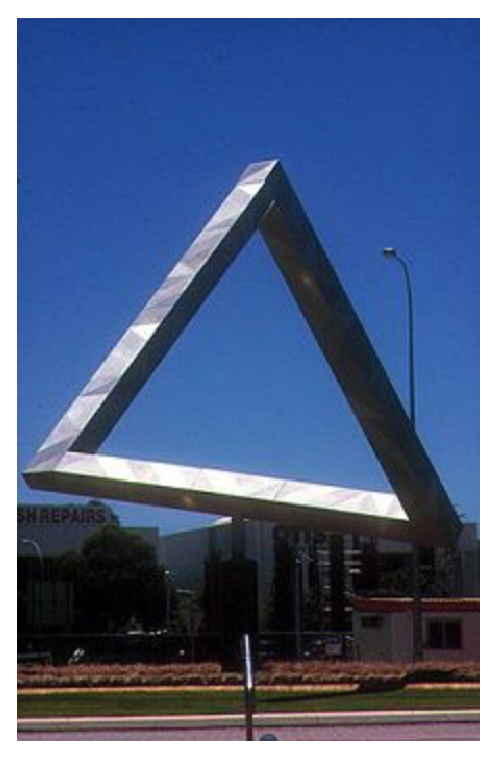
\includegraphics[height=3.5cm]{Penrose3}
\end{center}

}
%\themaO
\graphicspath{{../../S10_Probabilites/Images/}}

\chapter{Probabilités}
\label{S10}


%%%%%%%%%%%%%%%%%%%%%%%%%%%%%%%%%%%%%%%%%%
\begin{prerequis}
   \begin{itemize}
      \item Vocabulaire des probabilités.
      \item Notion de probabilités.
      \item La probabilité d’un événement est comprise entre 0 et 1.
      \item[\com] Aborder les questions relatives au hasard à partir de problèmes simples.
      \item[\com] Calculer des probabilités dans des cas simples.
   \end{itemize}
\end{prerequis}

\vfill

\begin{debat}[Débat : histoire des probabilités] 
   C’est en cherchant à résoudre des problèmes posés par les jeux de hasard que les mathématiciens donnent naissance aux {\bf probabilités}. Lors de fouilles archéologiques, on a trouvé des indices montrant que les jeux de hasard se pratiquaient déjà 5\,000 ans av. J.-C. (on utilisait des osselets). Les premiers dés connus ont été mis à jour à {\it Tepe Gawra}, au nord de l’Irak, et datent du troisième millénaire av. J.-C. Le jeu de cartes était également pratiqué dans divers pays depuis des époques reculées. Les cartes actuelles apparaissent en France au {\small XIV}\up{e} siècle et leur utilisation donne très vite lieu à des jeux d’argent. \\
   On attribue souvent la réelle naissance à la fin du {\small XVII}\up{e} siècle ce qui en fait une branche des mathématiques relativement récente.
   \begin{center}
      \begin{pspicture}(1,0)(8,3)
         \rput(2,1){\psdice[linecolor=G1]{6}}
         \rput(5,2){\psdice[linecolor=A1]{5}}
         \rput(4,0.5){\psdice[linecolor=B1]{4}}
         \rput(7,2.5){\psdice[linecolor=J1]{3}}
         \rput(6,0.75){\psdice[linecolor=gray]{2}}
         \rput(3,2.5){\psdice[linecolor=H1]{1}}
      \end{pspicture}
   \end{center}
   \bigskip
   \begin{cadre}[B2][F4]
      \begin{center}
         Vidéo : \href{https://leblob.fr/fondamental/les-probabilites}{\bf Les probabilités}, site Internet {\it Le blob}, épisode des {\it Petits contes mathématiques}.
      \end{center}
   \end{cadre}
\end{debat}

\vfill

\textcolor{PartieGeometrie}{\sffamily\bfseries Cahier de compétences} : chapitre 6, exercices 27 à 36.


%%%%%%%%%%%%%%%%%%%%%%%%%%%%%%%%%%%%%
%%%%%%%%%%%%%%%%%%%%%%%%%%%%%%%%%%%%%
\activites

\begin{activite}[Imposible, probable o seguro]
   {\bf Objectifs} : placer un événement sur une échelle de probabilité. 
   \begin{QCM}
      \partie[traduction]
         Traduire en français les six vignettes de cette illustration.
         \begin{center}
            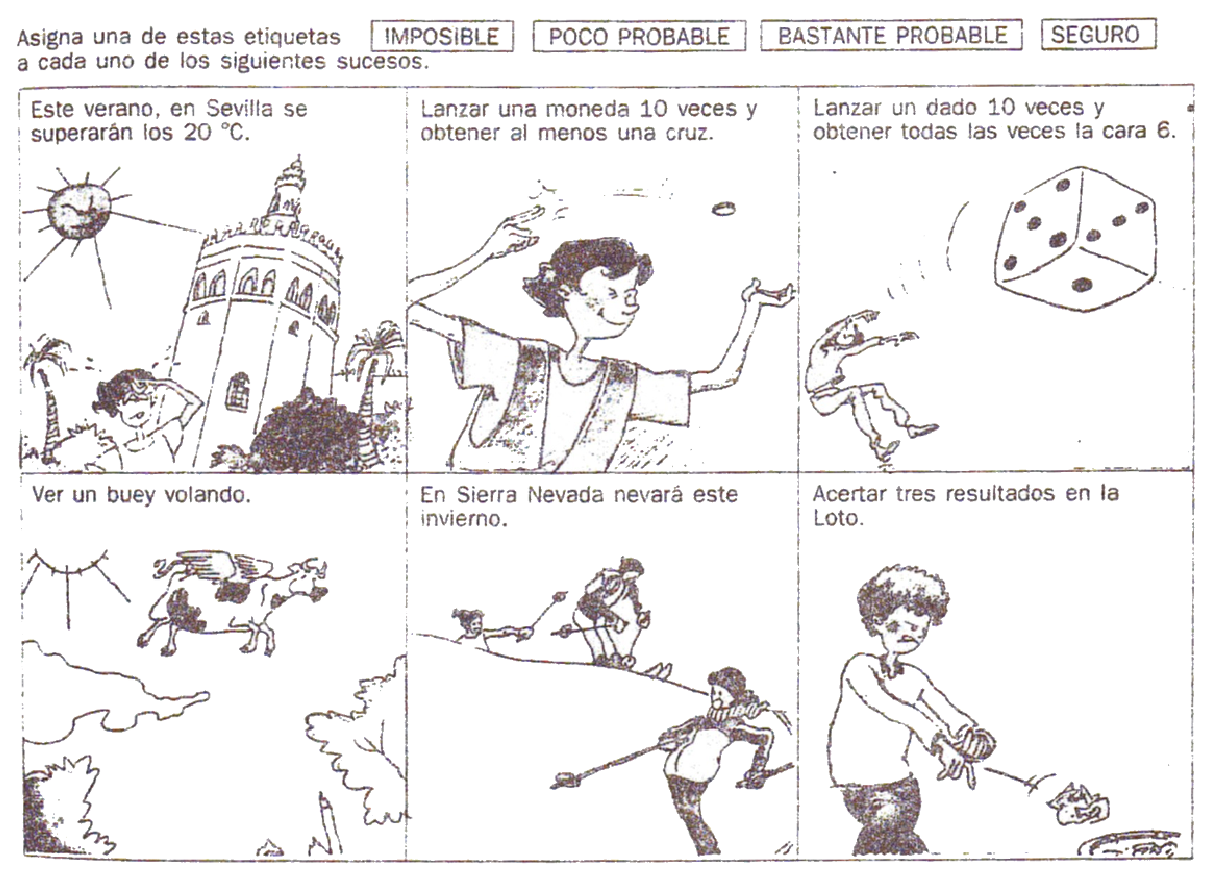
\includegraphics[width=14cm]{BD}
        \end{center}
        \ \\ [-10mm]
        \begin{itemize}
           \item Vignette 1 : \pfb \medskip
           \item Vignette 2 : \pfb \medskip
           \item Vignette 3 : \pfb \medskip
           \item Vignette 4 : \pfb \medskip
           \item Vignette 5 : \pfb \medskip
           \item Vignette 6 : \pfb \bigskip
        \end{itemize}
     \partie[exploitation]
        Pour chaque cas, dire si l'affirmation est \og imposible \fg, \og poco probable \fg, \og bastante probable \fg{} ou \og seguro \fg.
        \begin{center}
           {\hautab{1.4}
           \begin{ltableau}{0.9\linewidth}{6}
              \hline
              Vignette 1 & Vignette 2 & Vignette 3 & Vignette 4 & Vignette 5 & Vignette 6 \\
              \hline
              & & & & & \\
              \hline
           \end{ltableau}}
        \end{center}
        \bigskip
   \end{QCM}
   \medskip
   \vfill\hfill {\it\footnotesize Source : \href{http://numerisation.irem.univ-mrs.fr/RO/IRO09001/IRO09001.pdf}{Une initiation aux probabilités par le jeu}, IREM de Rouen.}
\end{activite}


%%%%%%%%%%%%%%%%%%%%%%%%%%%%%%%%%%%%%
%%%%%%%%%%%%%%%%%%%%%%%%%%%%%%%%%%%%%
\cours 

\section{Vocabulaire des probabilités} %%%

\begin{definition}
   On appelle \textbf{expérience aléatoire} une expérience dont on ne peut pas prévoir le résultat de façon certaine.
\end{definition}

\begin{exemple*1}
   Lancer une pièce de monnaie est une expérience aléatoire dont le résultat est soit \og pile \fg, soit \og face \fg.
\end{exemple*1}

\begin{vocabulaire}
   \begin{itemize}
      \item Chaque résultat possible et prévisible d'une expérience aléatoire est appelé une \textbf{issue}.
      \item L'ensemble formé par les issues est appelé \textbf{univers}, souvent noté $\Omega$.
      \item Un \textbf{événement} de l'expérience aléatoire est une partie quelconque de l'univers.
   \end{itemize}
\end{vocabulaire}

\begin{exemple*1}
   \begin{itemize}
      \item Lancer d'une pièce de monnaie : $\Omega =\{$~pile~;~face~$\}$.
      \item Lancer d'un dé à six faces : $\Omega =\{~1~;~2~;~3~;~4~;~5~;~6~\}$. \\
      \og Obtenir un numéro pair \fg{} est un événement que l'on peut noter $A=\{~2~;~4~;~6~\}$.
   \end{itemize}
   \vspace*{-5mm}
\end{exemple*1}


\section{Calcul de probabilités} %%%

La probabilité $P$ d'un événement est \og la chance \fg{} qu'il se produise.

\begin{definition}
   On dit qu'il y a \textbf{équiprobabilité} lorsque toutes les issues ont la même probabilité ; \\ [0.5mm]
   dans ce cas, on a $P=\dfrac{\textrm{nombre d'issues favorables}}{\textrm{nombre de cas possibles}}$.
\end{definition}

\begin{remarque}
   dans un exercice, pour signifier que l'on est dans une situation d'équiprobabilité, on a des expressions du type : \og on lance un dé \textbf{non pipé} \fg ; \og dans une urne, les boules sont \textbf{indiscernables} au toucher \fg ; \og on rencontre \textbf{au hasard} une personne parmi\dots \fg.
\end{remarque}

\begin{exemple}
   On tire une carte dans un jeu non truqué de 52 cartes. Quelle est la probabilité d'obtenir une tête ?
   \correction
      Le jeu est non truqué, il y a donc équiprobabilité. Les issues possibles sont le valet, la dame et le roi de pique, de carreau, de trèfle et de coeur ce qui fait $4\times3$ cartes donc, $P =\dfrac{12}{52}$.
\end{exemple}

\begin{propriete}
   Un probabilité est toujours comprise entre 0 et 1. Si elle est égale à 0, on dit que l'événement est {\bf impossible} et si elle est égale à 1, l'événement est {\bf certain}.
\end{propriete}

\begin{exemple}
   On lance un dé classique équilibré à six faces. Quelle est la probabilité d'obtenir un 9 ? d'obtenir un nombre entier ?
\correction
   Nous sommes dans une situation d'équiprobabilité.
   \begin{itemize} 
      \item On ne peut pas obtenir un 9 avec un dé à 6 faces donc, $P =\dfrac06 =0$.
      \item Tous les nombres obtenus sont entiers donc, $P =\dfrac66 =1$.
   \end{itemize}
\end{exemple}



%%%%%%%%%%%%%%%%%%%%%%%%%%%%%%%%%%%
%%%%%%%%%%%%%%%%%%%%%%%%%%%%%%%%%%%
\exercicesbase

\begin{colonne*exercice}

\serie{Échelle des probabilités} %%%

\begin{exercice} %1
   Pour chacun des événements suivants, indiquer s'il relève du hasard et si oui, le placer sur l'échelle ci-dessous.
   \begin{center}
      \begin{pspicture}(0,-0.5)(8,0.5)
         \psline{->}(0.3,0)(7.7,0)
         \rput(4,0){|}
         \footnotesize
         \rput{90}(0.1,-0.2){impossible}
         \rput{90}(7.9,0){certain}
         \rput(1.2,0.3){improbable}
         \rput(3,0.3){peu probable}
         \rput(4.8,0.3){probable}
         \rput(6.5,0.3){très probable}
      \end{pspicture}
   \end{center}
   \begin{enumerate}
      \item Obtenir pile au jeu de pile ou face \pfb
      \item La fête nationale aura lieu le 14 juillet \pfb
      \item Un élève aura des basquettes demain \pfb
      \item Obtenir 6 avec un dé à six faces \pfb
      \item Trouver la bonne combinaison au loto \pfb
      \item Demain il fera beau \pfb
   \end{enumerate}
\end{exercice}

\begin{corrige}
   \ \\ [-5mm]
   \begin{enumerate}
      \item Obtenir pile au jeu de pile ou face : {\blue hasard}.
      \item La fête nationale aura lieu le 14 juillet.
      \item Un élève aura des basquettes demain : {\blue hasard}.
      \item Obtenir 6 avec un dé à six faces : {\blue hasard}.
      \item Trouver la bonne combinaison au loto : {\blue hasard}.
      \item Demain il fera beau : {\blue hasard}.
   \end{enumerate}
   \begin{pspicture}(0.7,-0.9)(8,0.9)
      \psline{->}(0.3,0)(7.7,0)
      \rput(4,0){|}
      \footnotesize
      \rput{90}(0.1,0){impossible}
      \rput{90}(7.9,0){certain}
      \rput(1.2,0.3){improbable}
      \rput(3,0.3){peu probable}
      \rput(4.8,0.3){probable}
      \rput(6.5,0.3){très probable}
      \rput(5,-0.4){\blue 1}
      \rput(7.7,-0.4){\blue 2}
      \rput(6,-0.4){\blue 3}
      \rput(3,-0.4){\blue 4}
      \rput(1,-0.4){\blue 5}
      \rput(3.9,-0.4){\blue 6}
   \end{pspicture}
\end{corrige}


\begin{exercice} %2
   Une roue de loterie est partagée en huit secteurs identiques numérotés de 1 à 8. Calculer la probabilité de chaque événement et les placer sur l'échelle.
   \begin{center}
      \begin{pspicture}(0.7,-0.5)(8,1)
         \psline{->}(0.3,0)(7.7,0)
         \rput(4,0){|}
         \footnotesize
         \rput{90}(0.1,-0.2){impossible}
         \rput{90}(7.9,0){certain}
         \rput(1.2,0.3){improbable}
         \rput(3,0.3){peu probable}
         \rput(4.8,0.3){probable}
         \rput(6.5,0.3){très probable}
      \end{pspicture}
   \end{center}
   \begin{enumerate}
      \item \og Obtenir 2. \fg
      \item \og Obtenir un multiple de 2. \fg
      \item \og Obtenir un nombre supérieur à 4. \fg
      \item \og Obtenir un nombre positif. \fg
      \item \og Obtenir un nombre impair. \fg
      \item \og Obtenir un multiple de 13. \fg
   \end{enumerate}
\end{exercice}

\begin{corrige}
   \ \\ [-5mm]
   \begin{enumerate}
      \item Obtenir 2 : $\blue P =1/8$
      \item Obtenir un multiple de 2 : $\blue P =4/8$
      \item Obtenir un nombre supérieur à 5 : $\blue P =3/8$
      \item Obtenir un nombre positif : $\blue P =8/8 =1$
      \item Obtenir un nombre impair : $\blue P =4/8$
      \item Obtenir un multiple de 13 : $\blue P =0/8 =0$
   \end{enumerate}
   \begin{pspicture}(0.7,-1)(8,0.9)
      \psline{->}(0.3,0)(7.7,0)
      \rput(4,0){|}
      \footnotesize
      \rput{90}(0.1,0){impossible}
      \rput{90}(7.9,0){certain}
      \rput(1.2,0.3){improbable}
      \rput(3,0.3){peu probable}
      \rput(4.8,0.3){probable}
      \rput(6.5,0.3){très probable}
      \rput(3,-0.4){\blue 1}
      \rput(5,-0.4){\blue 2 et 5}
      \rput(4,-0.4){\blue 3}
      \rput(7.5,-0.4){\blue 4}
      \rput(0.5,-0.4){\blue 6}
   \end{pspicture}
\end{corrige}


\serie{Calcul de probabilités} %%%

\medskip

\begin{exercice} %3
   On écrit sur les faces d’un dé équilibré à six faces, chacune des lettres du mot : NOTOUS. On lance le dé et on regarde la lettre inscrite sur la face supérieure.
   \begin{enumerate}
      \item Quelles sont les issues de cette expérience ?
      \item Déterminer la probabilité des évènements suivants :
      \begin{enumerate}
         \item $E_1$ : \og On obtient la lettre O. \fg
         \item $E_2$ : \og On obtient une consonne. \fg
         \item $E_3$ : \og On obtient une lettre du mot KIWI. \fg
         \item $E_4$ : \og On obtient une lettre du mot CAGOUS. \fg
      \end{enumerate}
      \item Graduer un axe et y placer les probabilités des évènements précédents.
   \end{enumerate}
\end{exercice}

\begin{corrige}
   \ \\ [-5mm]
   \begin{enumerate}
      \item Les issues possibles sont les lettres {\blue N, O, T, U, S}
      \item
      \begin{enumerate}
         \item $E_1=\{\text{O}\}$ (lettre double) donc, $\blue P(E_1) =\dfrac26$
         \item  $E_2=\{\text{N, T, S}\}$ donc, $\blue P(E_2) =\dfrac36$
         \item  $E_3=\{\varnothing\}$ donc, $\blue P(E_3) =\dfrac06 =0$
         \item  $E_4=\{\text{O, U, S}\}$ donc, $\blue P(E_4) =\dfrac46$
      \end{enumerate}
      \setcounter{enumi}{2}
      \item Axe de graduation : \\
      \begin{pspicture}(0.7,-1)(8,0.9)
         \psline{->}(0.3,0)(7.7,0)
         \rput(4,0){|}
         \footnotesize
         \rput{90}(0.1,0){impossible}
         \rput{90}(7.9,0){certain}
         \rput(1.2,0.3){improbable}
         \rput(3,0.3){peu probable}
         \rput(4.8,0.3){probable}
         \rput(6.5,0.3){très probable}
         \rput(3.5,-0.5){\blue $E_1$}
         \rput(4.5,-0.5){\blue $E_2$}
         \rput(0.5,-0.5){\blue $E_3$}
         \rput(5.5,-0.5){\blue $E_4$}
      \end{pspicture}
   \end{enumerate}
\end{corrige}


\begin{exercice} %4
   Rosalie tire une carte dans un jeu ordinaire de cinquante-deux cartes.
   \begin{enumerate}
      \item Donner les probabilités de chacun des événements suivants : \og Obtenir un carreau \fg ; \og Obtenir un valet \fg{} et \og Obtenir un valet de carreau \fg.
      \item Calculer la probabilité de ne pas obtenir de carreau.
   \end{enumerate}
\end{exercice}

\begin{corrige}
   \ \\ [-5mm]
   \begin{enumerate}
      \item Obtenir un carreau : ${\blue P =\dfrac{13}{52}}$ \\ [1mm]
         Obtenir un valet : ${\blue P =\dfrac{4}{52}}$ \\
         Obtenir un valet de carreau  : ${\blue P =\blue \dfrac{1}{52}}$ \smallskip
      \item La probabilité de ne pas obtenir de carreau s'obtient en calculant la probabilité d'obtenir un c\oe ur, un pique ou un trèfle, ce qui fait au total $3\times13$ carte, soit 39 cartes. {\blue $P =\dfrac{39}{52}$}.
   \end{enumerate}      
\end{corrige}

\medskip


\begin{exercice} %5
   On dispose d’un dé à six faces numérotées de 1 à 6 et d’un dé à quatre faces avec des sommets numérotés de 1 à 4, parfaitement équilibrés. On lance les deux dés.
   \begin{enumerate}
      \item Avec quel dé la probabilité d’obtenir un 3 est-elle la plus
grande ?
      \item Avec quel dé la probabilité d’obtenir un multiple de 3 est-elle la plus grande ?
   \end{enumerate}
\end{exercice}

\begin{corrige}
   \ \\ [-5mm]
   \begin{enumerate}
      \item Dé à six faces : $P =\dfrac16$ (obtenir 3) ; \\ [1mm]
      dé à quatre faces : $P =\dfrac14$ (obtenir 3). \\ [1mm]
      C'est avec le {\blue dé à quatre faces} que la probabilité d'obtenir un 3 est la plus grande. \smallskip
      \item Dé à six faces : $ P =\dfrac26$ (obtenir 3 ou 6) ; \\ [1mm]
      dé à quatre faces : $P =\dfrac14$ (obtenir 3). \\ [1mm] 
      C'est avec le {\blue dé à six faces} que la probabilité d'obtenir un multiple de 3 est la plus grande.
   \end{enumerate}
\end{corrige}

\medskip


\begin{exercice} %6
   Trois personnes, Ali, Ben et Charles, ont chacune un sac contenant des billes. Chacune tire au hasard une bille de son sac dont le contenu est le suivant : \\ [1mm]
      {\hautab{1.25}
      \begin{ltableau}{\linewidth}{3}
         \hline
         Sac d'Ali & Sac de Ben & Sac de Charles \\
         \hline
         10 billes rouges & 97 billes rouges & 5 billes rouges \\
         30 billes noires & 3 billes noires & \\
         \hline
      \end{ltableau}}
   Laquelle de ces trois personnes a-t-elle la plus grande probabilité de tirer une bille rouge ? Justifier.
\end{exercice}

\begin{corrige}
   probabilité de tirer une bille rouge :
   \begin{itemize}
      \item Pour Ali : $P =\dfrac{10}{40} =0,25$. \smallskip
      \item Pour Ben : $P =\dfrac{97}{100} =0,97$. \smallskip
      \item Pour Charles : $P =\dfrac{5}{5} =1$. \smallskip
   \end{itemize}
  {\blue Charles a la plus grande probabilité d'obtenir une bille rouge}, ce qui est logique puisqu'il n'a QUE des billes rouges. \\
\end{corrige}

\medskip


\begin{exercice} %7
   Dans une loterie, 300 billets sont vendus et il y a 37 billets gagnants. Les autres billets sont des billets perdants. Parmi les 37 billets gagnants :
   \begin{itemize}
      \item 2 de ces billets permettent de gagner une télévision ;
      \item 5 permettent de gagner un bon de \ueuro{100} ;
      \item 10 permettent de gagner un bon de \ueuro{50} ;
      \item 20 permettent de gagner un porte-clés.
   \end{itemize}
   \vspace*{-5mm}
   \begin{enumerate}
      \item Quelle est la probabilité de gagner une télévision si l’on achète un billet ?
      \item Quelle est la probabilité de gagner un bon (peu importe la somme) si l’on achète un billet ?
      \item En plus de l’achat des bons dans plusieurs magasins, l’organisateur de la loterie dépense \ueuro{500} pour chaque télévision et \ueuro{0,50} pour chaque porte-clés.
      \begin{enumerate}
         \item À quel prix doit-il vendre les billets de loterie pour être sûr que ce jeu ne lui fera pas perdre d’argent ?
         \item S’il souhaite vendre chaque billet \ueuro{2}, combien doit-il rajouter de billets perdants pour être assuré que ce jeu ne lui fera pas perdre d’argent ? \\ [-10mm]
      \end{enumerate}
   \end{enumerate}
\end{exercice}

\begin{corrige}
   \ \\ [-5mm]
   \begin{enumerate}
   \item $P =\dfrac{2}{300}$. La probabilité de gagner une télévision est de {\blue $\dfrac{2}{300} \approx0,007$}. \smallskip
   \item $P =\dfrac{5+10}{300} =\dfrac{15}{300}$. La probabilité de gagner un bon de réduction est de {\blue $\dfrac{15}{300} =0,05$}. \smallskip
   \item
   \begin{enumerate}
      \item Calcul des dépenses $D$ de l'organisateur : \\
      $2\times\ueuro{500}+5\times\ueuro{100}+10\times\ueuro{50} +20\times\ueuro{0,50}$ \\
      $D =\ueuro{2010}$. Or, $\ueuro{2010}\div300 =\ueuro{6,7}$ donc, si l'organisateur vend 300 billets, {\blue il devra les vendre au minimum à 6,70 \euro{}} pour ne pas perdre d'argent.
      \item Il a dépensé \ueuro{2010}, et la vente de ses 300 billets à \ueuro{2} lui rapporte \ueuro{600}. Il lui reste alors $\ueuro{2010}-\ueuro{600} =\ueuro{1410}$ à récupérer. \\
      Or, $\ueuro{1410}\div\ueuro{2} =705$. \\
      Donc, à \ueuro{2}, {\blue l'organisateur doit ajouter au moins 705 billets} pour ne pas perdre d'argent. \\
   \end{enumerate}
\end{enumerate}

\bigskip
\corec{Vers la loi des grands nombres\dots}
\medskip

   \begin{ltableau}{\linewidth}{7}
      \hline
      N° & 1 & 2 & 3 & 4 & 5 & 6 \\
      \hline
      \small Proba & 1/6 & 1/6 & 1/6 & 1/6 & 1/6 & 1/6 \\
      \hline
      \small Proba & $0,17$ & $0,17$ & $0,17$ & $0,17$ & $0,17$ & $0,17$ \\
      \hline
   \end{ltableau}
   Les probabilités, en théorie, sont toutes identiques.
\end{corrige}

\end{colonne*exercice}


%%%%%%%%%%%%%%%%%%%%%%%%%%%%%%%%%%%
%%%%%%%%%%%%%%%%%%%%%%%%%%%%%%%%%%%
\Recreation

\enigme[Vers la loi des grands nombres\dots]

Le travail s'effectue en binôme, vous avez à votre disposition un dé classique non truqué à six faces.

{\hautab{1.6}
\begin{enumerate}
   \item Compléter le tableau suivant : \\ [1mm] 
   \begin{Ltableau}{0.95\linewidth}{7}{c}
      \hline
      Numéro sur la face visible du dé & 1 & 2 & 3 & 4 & 5 & 6 \\
      \hline
      Probabilité d'obtenir cette face (fraction) & & & & & & \\
      \hline
      Probabilité d'obtenir cette face (décimal) & & & & & & \\
      \hline
   \end{Ltableau} \bigskip
   Que remarque-t-on ? \pfb \\
   \item Lancer 10 fois le dé et noter les résultats obtenus dans le tableau suivant : \\ [1mm]
   \begin{Ltableau}{0.95\linewidth}{7}{c}
      \hline
      Numéro sur la face visible du dé & 1 & 2 & 3 & 4 & 5 & 6 \\
      \hline
      Nombre de fois où cette face est obtenue & & & & & & \\
      \hline
      Probabilité d'obtenir cette face (fraction) & & & & & & \\
      \hline
      Probabilité d'obtenir cette face (décimal) & & & & & & \\
      \hline
   \end{Ltableau} \bigskip
   Que remarque-t-on ? \pfb \\
   \item Lancer 100 fois le dé et noter les résultats obtenus dans le tableau suivant : \\ [1mm]
   \begin{Ltableau}{0.95\linewidth}{7}{c}
      \hline
      Numéro sur la face visible du dé & 1 & 2 & 3 & 4 & 5 & 6 \\
      \hline
      Nombre de fois où cette face est obtenue & & & & & & \\
      \hline
      Probabilité d'obtenir cette face (fraction) & & & & & & \\
      \hline
      Probabilité d'obtenir cette face (décimal) & & & & & & \\
      \hline
   \end{Ltableau} \bigskip
   Que remarque-t-on ? \pfb \\
   \item Répertorier les résultats de la classe entière et noter les résultats obtenus dans le tableau suivant : \\ [1mm]
   \begin{Ltableau}{0.95\linewidth}{7}{c}
      \hline
      Numéro sur la face visible du dé & 1 & 2 & 3 & 4 & 5 & 6 \\
      \hline
      Nombre de fois où cette face est obtenue & & & & & & \\
      \hline
      Probabilité d'obtenir cette face (fraction) & & & & & & \\
      \hline
      Probabilité d'obtenir cette face (décimal) & & & & & & \\
      \hline
   \end{Ltableau} \bigskip
   Que remarque-t-on ? \pfb
\end{enumerate}}


%\setlength{\doublerulesep}{0.3pt}

\themaN
\graphicspath{{../../S11_Multiples_et_diviseurs/Images/}}

\chapter{Multiples et diviseurs}
\label{S11}


%%%%%%%%%%%%%%%%%%%%%%%%%%%%%%%%%%%%%%%%%%
%%%%%%%%%%%%%%%%%%%%%%%%%%%%%%%%%%%%%%%%%%
\begin{prerequis}[Connaissances $\heartsuit$ et compétences $\diamondsuit$ du cycle 4]
   \begin{itemize}
      \item Multiples et diviseurs.
      \item Critères de divisibilité par 2, 3, 5, 9.
      \item Division euclidienne.
      \item[\com] Déterminer si un entier est ou n'est pas multiple ou diviseur d'un autre entier.
      \item[\com] Utiliser un critère de divisibilité par 2, 3, 5, 9, 10.
      \item[\com] Modéliser et résoudre des problèmes mettant en jeu la divisibilité.
   \end{itemize}
\end{prerequis}

\vfill

\begin{debat}[Débat : la division euclidienne] 
   Le nom de {\bf division euclidienne} est un hommage rendu à {\it Euclide} (300 av. J.-C.), mathématicien grec qui en explique le principe par soustractions successives dans son \oe uvre {\it Les éléments}. Mais elle apparait très tôt dans l'histoire des mathématiques, par exemple dans les mathématiques égyptiennes, babyloniennes et chinoises.
   \begin{center}
      \begin{pspicture}(0,1)(4,4.5)
         \psline[linewidth=1mm](2,1)(2,4)
         \psline[linewidth=1mm](2,3)(4,3)
         \textcolor{B1}{\it\large
         \rput(0.8,3.5){dividende}
         \rput(3,3.5){diviseur}
         \rput(3,2.5){quotient}
         \rput(3,2){\small (euclidien)}
         \rput(1,1.5){reste}}
      \end{pspicture}
   \end{center}
   \bigskip
   \begin{cadre}[B2][F4]
      \begin{center}
         Vidéo : \href{https://www.youtube.com/watch?v=VWS9NyXbEyY&t=18s}{\bf Division euclidienne avec matériel multibase}, chaîne YouTube {\it Méthode Heuristique}.
      \end{center}
   \end{cadre}
\end{debat}

\vfill

\textcolor{PartieGeometrie}{\sffamily\bfseries Cahier de compétences} : $\varnothing$


%%%%%%%%%%%%%%%%%%%%%%%%%%%%%%%%%%
%%%%%%%%%%%%%%%%%%%%%%%%%%%%%%%%%%
\activites

\begin{activite}[Les multiplications incomplètes]
   {\bf Objectifs} : calculer mentalement des multiplications et des divisions ; résoudre un problème de calcul mental ; compléter un tableau à double entrée.
   \begin{QCM}
   Compléter ces tables de multiplication dont on a effacé le contenu de certaines cases. Les nombres sont tous strictement positifs, il ne peut pas y avoir deux fois le même nombre sur une même colonne ou une même ligne. \medskip
   {\hautab{1.82}
   \partie[piste verte] \medskip
      \hfill
      \begin{tabular}{|C{0.5}||C{0.5}|C{0.5}|}
         \hline
         {\Large $\times$} & & \\
         \hline\hline
         & & 24 \\
         \hline
         & 25 & 30 \\
         \hline
      \end{tabular}
      \hfill
      \begin{tabular}{|C{0.5}||C{0.5}|C{0.5}|}
         \hline
         {\Large $\times$} & & 7 \\
         \hline\hline
         & & 21 \\
         \hline
         4 & 8 & \\
         \hline
      \end{tabular}
      \hfill
      \begin{tabular}{|C{0.5}||C{0.5}|C{0.5}|}
         \hline
         {\Large $\times$} & 6 & \\
         \hline\hline
         & 24 & 32 \\
         \hline
         & 36 & \\
         \hline
      \end{tabular}
      \hfill
      \begin{tabular}{|C{0.5}||C{0.5}|C{0.5}|}
         \hline
         {\Large $\times$} & 3 & \\
         \hline\hline
         & & 18 \\
         \hline
         5 & & 45 \\
         \hline
      \end{tabular}
      \hspace*{1cm} \\
         
   \partie[piste bleue] \medskip
      \hfill
      \begin{tabular}{|C{0.5}||C{0.5}|C{0.5}|C{0.5}|}
         \hline
         {\Large $\times$} & 2 & & \\
         \hline\hline
         & & 9 & \\
         \hline
         & 8 & & \\
         \hline
         & 16 & & 56 \\
         \hline
      \end{tabular}
      \hfill
      \begin{tabular}{|C{0.5}||C{0.5}|C{0.5}|C{0.5}|}
         \hline
         {\Large $\times$} & 2 & & \\
         \hline\hline
         4 & & 16 & \\
          \hline
         & & & 35 \\
         \hline
         9 & 18 & & 45 \\
         \hline
      \end{tabular}
      \hfill
      \begin{tabular}{|C{0.5}||C{0.5}|C{0.5}|C{0.5}|}
         \hline
         {\Large $\times$} & & 7 & \\
         \hline\hline
         & 12 & & 32 \\
         \hline
         & & & 64 \\
         \hline
         & & 63 & 72 \\
         \hline
      \end{tabular}
      \hspace*{1cm} \\
      
   \partie[piste rouge] \medskip 
      \hfill
      \begin{tabular}{|C{0.5}||C{0.5}|C{0.5}|C{0.5}|}
         \hline
         {\Large $\times$} & & 3 & \\
         \hline\hline
         & 20 & & \\
         \hline
         & & 18 & \\
         \hline
         & & 6 & 4 \\
         \hline
      \end{tabular}
      \hfill
      \begin{tabular}{|C{0.5}||C{0.5}|C{0.5}|C{0.5}|}
         \hline
         {\Large $\times$} & & & 7 \\
         \hline\hline
         2 & & & 14 \\
         \hline
         & 72 & 54 & \\
          \hline
         & 40 & & 35 \\
         \hline
      \end{tabular}
      \hfill
      \begin{tabular}{|C{0.5}||C{0.5}|C{0.5}|C{0.5}|}
         \hline
         {\Large $\times$} & & & \\
         \hline\hline
         & 18 & & 15 \\
         \hline
         & & 64 & \\
         \hline
         & & 32 & \\
         \hline
      \end{tabular}
      \hspace*{1cm} \\
      
   \partie[piste noire] \medskip
      \hfill
      \begin{tabular}{|C{0.5}||C{0.5}|C{0.5}|C{0.5}|}
         \hline
         {\Large $\times$} & & & 10 \\
         \hline\hline
         & 20 & 8 & \\
         \hline
         & 35 & & 70 \\
         \hline
         & & & 100 \\
         \hline
      \end{tabular}
      \hfill
      \begin{tabular}{|C{0.5}||C{0.5}|C{0.5}|C{0.5}|}
         \hline
         {\Large $\times$} & & & \\
         \hline\hline
         & & 45 & \\
         \hline
         & 28 & & \\
         \hline
         & 44 & & 99 \\
         \hline
      \end{tabular}
      \hfill
      \begin{tabular}{|C{0.5}||C{0.5}|C{0.5}|C{0.5}|}
         \hline
         {\Large $\times$} & & 13 & \\
         \hline\hline
         & & 65 & \\
         \hline
         & 42 & & 49 \\
         \hline
         & 72 & & 84 \\
         \hline
      \end{tabular}}
      \hspace*{1cm}
      \vspace*{1cm}
   \end{QCM}
\end{activite}


%%%%%%%%%%%%%%%%%%%%%%%%%%%%%%%%%%%%%%%%%%
%%%%%%%%%%%%%%%%%%%%%%%%%%%%%%%%%%%%%%%%%%
\cours 

%%%%%%%%%%%%%%%%%%%%%%%%%%
\section{Multiples et diviseurs}

\begin{minipage}{10cm}
   {\it Rappel :} effectuer une division euclidienne d'un {\bf dividende} $a$ par un {\bf diviseur} $b$, c'est trouver deux entiers appelés {\bf quotient} $q$ et {\bf reste} $r$ tels que $a=b\times q+r$ où $r<b$. \\
   Dans l'exemple ci-contre, on peut écrire : $123 =5\times24+3$.
\end{minipage}
\qquad
\begin{minipage}{4cm}
   \begin{pspicture}(-0.5,-0.5)(4,3)
      \rput(1,1.2){$\opidiv[displayintermediary=all,voperation=top]{123}{5}$}
      \psline[linecolor=A1]{->}(0.7,2.8)(0.7,2.4)
      \rput(0.7,3){\textcolor{A1}{dividende}}
      \psline[linecolor=A1]{<-}(1.9,2.3)(2.4,2.3)
      \rput[l](2.5,2.3){\textcolor{A1}{diviseur}}
      \psline[linecolor=B1]{<-}(2.2,1.7)(2.7,1.7)
      \rput[l](2.8,1.7){\textcolor{B1}{quotient}}
      \psline[linecolor=B1]{<-}(1.4,0.2)(1.9,0.2)
      \rput[l](2,0.2){\textcolor{B1}{reste}}
   \end{pspicture}
\end{minipage}

\begin{definition}
   $a$ et $b$ sont deux nombres entiers. Lorsque le reste de la division de $a$ par $b$ est égal à 0, on dit que $a$ est un \textbf{multiple} de $b$, ou que $b$ est un \textbf{diviseur} de $a$, ou encore que $a$ est \textbf{divisible} par $b$.
\end{definition}

\begin{exemple*1}
   \begin{itemize}
      \item 15 est un multiple de 3 car $15=3\times 5+\textcolor{A1}{0}$, on peut aussi dire que 3 est un diviseur de 15, ou que 15 est divisible par 3.
      \item 17 n'est pas un multiple de 3 car $17=3\times 5+\textcolor{A1}{2}$.
      \item Les diviseurs de 24 sont 1; 2; 3; 4; 6; 8; 12 et 24.
      \item Il y a une infinité de multiples de 18, comme par exemple 18 ; 36 ; 54 ; 180\dots
   \end{itemize}
   \vspace*{-3mm}
\end{exemple*1}

%%%%%%%%%%%%%%%%%%%%%%%%%%
\section{Critères de divisibilité}

\begin{propriete}
   \begin{itemize}
      \item un nombre est divisible par 2 s'il se termine par 0 ; 2 ; 4 ; 6 ou 8 ;
      \item un nombre est divisible par 3 si la somme de ses chiffres est un multiple de 3 ;
      \item un nombre est divisible par 5 s'il se termine par 0 ou 5 ;
      \item un nombre est divisible par 9 si la somme de ses chiffres est un multiple de 9 ;
      \item un nombre est divisible par 10 s'il se termine par 0.
   \end{itemize}
   \vspace*{-3mm}
\end{propriete}

\begin{exemple*1}
   \begin{itemize}
      \item 252 et 253 sont-ils divisibles par 3 ?
      \item 52\,362 et 52\,363 sont-ils divisibles par 9 ?
    \end{itemize}   
   \correction
      \begin{itemize}
         \item $2+5+2=9$ est multiple de 3 donc, 252 est divisible par 3. \\
            $2+5+3=10$ n'est pas multiple de 3 donc, 253 n'est pas divisible par 3.
         \item $5+2+3+6+2=18$ est multiple de 9 donc, 52\,362 est divisible par 9, et donc par 3. \\
            $5+2+3+6+3=19$ n'est pas multiple de 9 donc, 52\,363 n'est pas divisible par 9.
       \end{itemize}
    \vspace*{-3mm}
\end{exemple*1}

\begin{remarque}
   pour savoir si un nombre est divisible par $3$, on peut calculer la somme des chiffres du nombre obtenu jusqu'à ce que l'on trouve un seul chiffre : \\
   pour $563\,387\,981$, on calcule : $5+6+3+3+8+7+9+8+1=50$. Puis on calcule $5+0=5$.
   $5$ n'est pas divisible par $3$ donc, $563\,387\,981$ n'est pas divisible par $3$.
\end{remarque}



%%%%%%%%%%%%%%%%%%%%%%%%%%%%%%%%%%%%%
%%%%%%%%%%%%%%%%%%%%%%%%%%%%%%%%%%%%%
\exercicesbase

\begin{colonne*exercice}

\serie{Division euclidienne} %%%

\bigskip

\begin{exercice} %1
   Effectuer la division euclidienne de 307 par 7 puis de 13\,758 par 25.
\end{exercice}
        
\begin{corrige}
   {\small \opidiv[displayintermediary=all,voperation=top]{307}{7} \qquad \opidiv[displayintermediary=all,voperation=top]{13758}{25}} \\
   {\blue $307 =7\times43+6$} et {\blue $13\,758 =25\times550+8$}.
\end{corrige}

\bigskip


\begin{exercice} %2
   On donne les égalités : \\
   $415 = 7\times59+2$ \; et \; $56\times57 = 3\,192$. \\
   Sans effectuer de calculs, donner le quotient et le reste des divisions euclidiennes suivantes.
   \begin{colenumerate}{2}
      \item 415 par 7
      \item 3\,192 par 56
      \item 415 par 59
      \item 3\,192 par 57
   \end{colenumerate}
\end{exercice}

\begin{corrige}
   \ \\ [-5mm]
   \begin{enumerate}
      \item Le quotient de 415 par 7 est {\blue 59}, le reste est {\blue 2}.
      \item Le quotient de 3\,192 par 56 est {\blue 57}, le reste est {\blue 0}.
      \item Le quotient de 415 par 59 est {\blue 7}, le reste est {\blue 2}.
      \item Le quotient de 3\,192 par 57 est {\blue 56}, le reste est {\blue 0}.
   \end{enumerate}
\end{corrige}

\bigskip


\begin{exercice} %3
   Résoudre les problèmes suivants :
   \begin{enumerate}
      \item 6\,798 supporters d'un club de rugby doivent faire un déplacement en car pour soutenir leur équipe. Chaque car dispose de 55 places. Combien de cars faut-il réserver ?
      \item Des stylos sont conditionnés par boîte de 40. Jules a 2\,647 stylos. Combien lui en manque-t-il pour avoir des boîtes entièrement remplies ?
      \item Trois amis participent à une chasse au trésor et trouvent 1\,419 pièces en chocolat. Si le partage est équitable, combien de pièces en chocolat auront-ils chacun ? Zakaria arrive et leur rappelle que c'est lui qui leur a prêté sa boussole. Il exige donc d'avoir la même part que chacun des trois autres plus les pièces restantes. Combien de pièces recevra-t-il ?
   \end{enumerate}
\end{exercice}

\begin{corrige}
   \ \\ [-5mm]
   \begin{enumerate}
      \item On effectue la division : {\small \opidiv[displayintermediary=all,voperation=top]{6798}{55}} \\
         Il faudra donc réserver {\blue 124 cars}.
      \item On effectue la division : {\small \opidiv[displayintermediary=all,voperation=top]{2647}{40}} \\
         Il lui reste 7 stylos pour une boite de 40, il faut donc ajouter {\blue 33 stylos} pour compléter la boite.
      \item On effectue la division : {\small \opidiv[displayintermediary=all,voperation=top]{1419}{3}} \\
         Chaque ami aura donc {\blue 473 pièces en chocolat}. \\
         Lorsque Zakaria arrive, on fait {\small \opidiv[displayintermediary=all,voperation=top]{1419}{4}} \\
         Il recevra $(354+3)$ pièces en chocolat, soit {\blue 357}.
   \end{enumerate}
\end{corrige}

\bigskip


%%%%%%%%%%%%%%%
\serie{Multiples et diviseurs}

\bigskip

 \begin{exercice} %7
   Trouver tous les diviseurs des nombres suivants : \\
   14 ; 40 ; 48 et 2\,037.
\end{exercice}

\begin{corrige}
   \begin{itemize}
      \item Diviseurs de 14 : {\blue 1 ; 2 ; 7 ; 14}.
      \item Diviseurs de 40 : {\blue 1 ; 2 ; 4 ; 5 ; 8 ; 10 ; 20 ; 40}.
      \item Diviseurs de 48 : {\blue 1 ; 2 ; 3 ; 4 ; 6 ; 8 ; 12 ; 16 ; 24 ; 48}.
      \item Diviseurs de 2\,037 : {\blue 1 ; 3 ; 7 ; 21 ; 97 ; 291 ; 679 ; 2037}.
   \end{itemize}
\end{corrige}

\bigskip


\begin{exercice} %5
   Ecrire :
   \begin{enumerate}
      \item La liste des dix premiers multiples de 6.
      \item Cinq multiples de 11.
      \item Tous les multiples de 13 inférieurs à 80.
      \item Le plus grand multiple de 12 inférieur à 75.
      \item Le plus grand multiple de 36 inférieur à 100.
      \item Le plus petit multiple de 9 supérieur à 1\,200.
      \item Le plus petit multiple de 14 supérieur à 710 ?
      \item Le plus petit et le plus grand diviseur de 2\,021.
   \end{enumerate}
\end{exercice}

\begin{corrige}
   \ \\ [-5mm]\begin{enumerate}
      \item Dix premiers multiples de 6 : \\
         {\blue 0 ; 6 ; 12 ; 18 ; 24 ; 30 ; 36 ; 42 ; 48 ; 54}.
      \item Cinq multiples de 11 : \\
         {\blue 0 ; 11 ; 22 ; 33 ; 44}.
      \item Multiples de 13 inférieurs à 80 : \\
         {\blue 0 ; 13 ; 26 ; 39 ; 52 ; 65 ; 78}
      \item Plus grand multiple de 12 inférieur à 75 : {\blue 72}.
      \item Plus grand multiple de 36 inférieur à 100 : {\blue 72}.
      \item Plus petit multiple de 9 supérieur à 1\,200 : {\blue 1206}.
      \item Plus petit multiple de 14 supérieur à 710 : {\blue 714}.
      \item Plus grand/petit diviseur de 2\,021 : {\blue 1 et 2\,021}.
   \end{enumerate}
\end{corrige}

\bigskip


\begin{exercice} %6
   Répondre aux questions suivantes :
   \begin{enumerate}
      \item 
      \begin{enumerate}
         \item Écrire tous les multiples de 3 inférieurs à 41. 
         \item Écrire tous les multiples de 5 inférieurs à 41.
         \item Entourer les multiples communs à 3 et 5.
         \item Que remarque-t-on ?
      \end{enumerate}
      \item
      \begin{enumerate}      
         \item Écrire tous les multiples de 4 inférieurs à 50. 
         \item Écrire tous les multiples de 6 inférieurs à 50.
         \item Entourer les multiples communs à 4 et 6.
         \item Que remarque-t-on ?
      \end{enumerate}
   \end{enumerate}
\end{exercice}

\begin{corrige}
   \ \\ [-5mm]
   \begin{enumerate}
      \item 
      \begin{enumerate}
         \item Multiples de 3 inférieurs à 41 : \\ \smallskip
            {\blue \fbox{0} ; 3 ; 6 ; 9 ; 12 ; \fbox{15} ; 18 ; 21 ; 24 ; 27 ; \fbox{30} ; 33 ; 36 ; 39} \smallskip
         \item Multiples de 5 inférieurs à 41 : \\ \smallskip
            {\blue \fbox{0} ; 5 ; 10 ; \fbox{15} ; 20 ; 25 ; \fbox{30} ; 35 ; 40} \smallskip
         \item On a entouré : {\blue 0 ; 15 ; 30}.
         \item On remarque que les multiples communs à 3 et à 5 sont les {\blue multiples de 15}.
      \end{enumerate}
      \setcounter{enumi}{1}
      \item
      \begin{enumerate}
         \item Multiples de 4 inférieurs à 50 : \\ \smallskip
            {\blue \fbox{0} ; 4 ; 8 ; \fbox{12} ; 16 ; 20 ; \fbox{24} ; 28 ; 32 ; \fbox{36} ; 40 ; 44 ; \fbox{\!48\!}} \smallskip
         \item Multiples de 6 inférieurs à 50 : \\ \smallskip
            {\blue \fbox{0} ; 6 ; \fbox{12} ; 18 ; \fbox{24} ; 30 ; \fbox{36} ; 42 ; \fbox{48}} \smallskip
         \item On a entouré : {\blue 0 ; 12 ; 24 ; 36 ; 48}.
         \item On remarque que les multiples communs à 4 et à 6 sont les {\blue multiples de 12}.
      \end{enumerate}
   \end{enumerate}
\end{corrige}

\bigskip


%%%%%%%%%%%%
\serie{Critères de divisibilité}

\bigskip

\begin{exercice} %8
   Les nombres 30 ; 27 ; 246 ; 325 ; 4\,238 et 6\,139 sont-ils divisibles par 2 ? par 3 ? par 5 ? par 9 ?
\end{exercice}

\begin{corrige}
   On résume les résultats dans un tableau : \\ \medskip
   {\hautab{1.25}
   \begin{CLtableau}{0.95\linewidth}{7}{c}
      \hline
      & 30 & 27 & 246 & 325 & 4\,238 & 6\,139 \\
      \hline
      par 2 & \textcolor{blue}{$\surd$} & & \textcolor{blue}{$\surd$} & & \textcolor{blue}{$\surd$} & \\
      \hline
      par 3 & \textcolor{blue}{$\surd$} & \textcolor{blue}{$\surd$} & \textcolor{blue}{$\surd$} & & & \\
      \hline
      par 5 & \textcolor{blue}{$\surd$} & & & \textcolor{blue}{$\surd$} & & \\
      \hline
      par 9 & & \textcolor{blue}{$\surd$} & & & & \\
      \hline
   \end{CLtableau}}
\end{corrige}

\bigskip


\begin{exercice} %9
   Colorie le chemin pour aller de la case 99 à la case 108 en ne passant que par des nombres divisibles par 9, horizontalement et verticalement. \\ [2mm]
   {\footnotesize
   \hautab{1.5}
   \begin{tabular}{C{0.25}|*{8}{C{0.43}|}C{0.3}}
      \cline{1-9}
      99 & 27 & 7875 & 934 & 117 & 9999 & 63 & 8321 & 69 & \\
       \cline{1-9}
      & 980 & 1116 & 128 & 9000 & 777 & 4455 & 109 & 675 & \\
      \cline{2-9}
      & 732 & 8784 & 666 & 7866 & 304 & 963 & 124 & 946 & \\
      \cline{2-9}
      & 132 & 678 & 418 & 456 & 2044 & 7272 & 1070 & 6666 & \\
      \cline{2-9}
      & 1152 & 4200 & 82 & 1035 & 3303 & 54 & 5543 & 765 & \\
      \cline{2-9}
      & 4778 & 354 & 4779 & 234 & 9001 & 1117 & 208 & 89 & \\
      \cline{2-9}
      & 810 & 888 & 7200 & 998 & 632 & 5544 & 36 & 945 & \\
      \cline{2-10}
      & 101 & 7001 & 6669 & 8757 & 207 & 1071 & 2350 & 2358 & 108 \\
      \cline{2-10}
   \end{tabular}}
\end{exercice}

\begin{corrige}
   Le chemin possible : \\ [1mm]
   {\footnotesize
   \hspace*{-10mm}
      {\hautab{1.5}
      \begin{tabular}{C{0.2}|*{8}{C{0.43}|}C{0.3}}
         \cline{1-9}
         \cellcolor{blue!25}{99} & \cellcolor{blue!25}{27} & \cellcolor{blue!25}{7875} & 934 & \cellcolor{blue!25}{117} & \cellcolor{blue!25}{9999} & \cellcolor{blue!25}{63} & 8321 & 69 & \\
         \cline{1-9}
         & 980 & \cellcolor{blue!25}{1116} & 128 & \cellcolor{blue!25}{9000} & 777 & \cellcolor{blue!25}{4455} & 109 & 675 & \\
         \cline{2-9}
         & 732 & \cellcolor{blue!25}{8784} & \cellcolor{blue!25}{666} & \cellcolor{blue!25}{7866} & 304 & \cellcolor{blue!25}{963} & 124 & 946 & \\
         \cline{2-9}
         & 132 & 678 & 418 & 456 & 2044 & \cellcolor{blue!25}{7272} & 1070 & 6666 & \\
         \cline{2-9}
         & 1152 & 4200 & 82 & \cellcolor{blue!25}{1035} & \cellcolor{blue!25}{3303} & \cellcolor{blue!25}{54} & 5543 & 765 & \\
         \cline{2-9}
         & 4778 & 354 & \cellcolor{blue!25}{4779} & \cellcolor{blue!25}{234} & 9001 & 1117 & 208 & 89 & \\
         \cline{2-9}
         & 810 & 888 & \cellcolor{blue!25}{7200} & 998 & 632 & \cellcolor{blue!25}{5544} & \cellcolor{blue!25}{36} & \cellcolor{blue!25}{945} & \\
         \cline{2-10}
         & 101 & 7001 & \cellcolor{blue!25}{6669} & \cellcolor{blue!25}{8757} & \cellcolor{blue!25}{207} & \cellcolor{blue!25}{1071} & 2350 & \cellcolor{blue!25}{2358} & \cellcolor{blue!25}{108} \\
         \cline{2-10}
      \end{tabular}}}
\end{corrige}

\bigskip


\begin{exercice} %9
   Je suis un nombre impair à deux chiffres sans 2 dans mon écriture. Je ne suis pas divisible par 5 mais je suis un multiple de 9. Qui suis-je ? 
\end{exercice}

\begin{corrige}
   \begin{itemize}
      \item On peut commencer par écrire la liste des multiples de 9 à deux chiffres : \\
         18 ; 27 ; 36 ; 45 ; 54 ; 63 ; 72 ; 81 ; 90 ; 99.
      \item On supprime ensuite les nombres pairs, il reste : \\
         27 ; 45 ; 63 ; 81 ; 99.
      \item On supprime 27 qui comporte un 2, il reste : \\
         45 ; 63 ; 81 ; 99. \\
      \item Enfin, on supprime 45 qui est divisible par 5. \\
         Je peux donc être {\blue 63, 81 ou 99}.
   \end{itemize}
\end{corrige}

\bigskip


\begin{exercice} %10
   Répondre par vrai ou faux en justifiant.
   \begin{enumerate}
      \item Tout nombre divisible par 3 est divisible par 9.
      \item Tout nombre divisible par 9 est divisible par 3.
      \item Tout nombre divisible par 2 et 3 est divisible par 5.
      \item Tout nombre dont le chiffre des unités est 2 est divisible par 2. 
      \item Tout nombre dont le chiffre des unités est 3 est divisible par 3.
   \end{enumerate}
\end{exercice}

\begin{corrige}
   \ \\ [-5mm]
   \begin{enumerate}
      \item Tout nombre divisible par 3 est divisible par 9 : \\
         {\blue faux}. \\
         Par exemple, 6 est divisible par 3 mais pas par 9.
      \item Tout nombre divisible par 9 est divisible par 3 : \\
         {\blue vrai}. \\
         Un nombre divisible par 9 s'écrit $9k$ où $k$ est un nombre entier. Or, $9k =3\times(3k)$ donc il est aussi divisible par 3.
      \item Tout nombre divisible par 2 et 3 est divisible par 5 : {\blue faux}. \\
      Par exemple, 6 est divisible par 2 et par 3 mais il n'est pas divisible par 5.
      \item Tout nombre dont le chiffre des unités est 2 est divisible par 2 : {\blue vrai}. \\
      Un nombre qui se termine par 0, 2, 4, 6 ou 8 est divisible par 2.
      \item Tout nombre dont le chiffre des unités est 3 est divisible par 3 : {\blue faux}. \\
      Par exemple, 13 se termine par 3 mais n'est pas divisible par 3.
   \end{enumerate}
   
\Coupe
\corec{L'escalier}
\medskip

\begin{enumerate}
      \item Le nombre de marches est un multiple de 3 inférieur à 100. Il peut donc être égal à : \\
      3;\;6;\;9;\;12;\;15;\;18;\;21;\;24;\;27;\;30;\;33;\;36;\;39;\\
      42;\;45;\;48;\;51;\;54;\;57;\;60;\;63;\;66;\;69;\;72;\;75;\\
      78;\;81;\;84;\;87;\;90;\;93;\;96;\;99. \\
      Le nombre de marches est un multiple de 4 inférieur à 100. Il peut donc être égal à : \\
      4;\;8;\;12;\;16;\;20;\;24;\;28;\;32;\;36;\;40;\;44;\;48;\\
      52;\;56;\;60;\;64;\;68;\;72;\;76;\;80;\;84;\;88;\;92;\;96. \\
      Le nombre de marches est un multiple de 5 inférieur à 100. Il peut donc être égal à : \\
      5;\;10;\;15;\;20;\;25;\;30;\;35;\;40;\;45;\;50;\;55;\;60;\\  
      65;\;70;\;75;\;80;\;85;\;90;\;95. \\
      Le nombre de marches doit faire partir des trois listes précédentes, le seul qui convient est 60. \\
      Conclusion : {\blue l'escalier comporte 60 marches}.
      \item 
      \begin{enumerate}
         \item Si on monte les marches 6 par 6, {\blue on arrive exactement sur la dernière marche} car $60 =10\times6$.
         \item Si on monte les marches 8 par 8, {\blue on n'arrive pas exactement sur la dernière marche} car \\
            $60 =7\times8+4$.
         \item Si on monte les marches alternativement par 5 puis par 7, {\blue on arrive exactement sur la dernière marche} car $60 =5\times(5+7)$.
         \item Si on monte les marches alternativement par 3 puis par 4, {\blue on n'arrive pas exactement sur la dernière marche} car $60 =8\times(3+4)+4$. \\
         En revanche, si on monte les marches alternativement par 4 puis par 3, {\blue on arrive exactement sur la dernière marche} car $60 =8\times(4+3)+4$.
      \end{enumerate}
   \end{enumerate}  
\end{corrige}
\vspace*{-2mm}
\flushright{\footnotesize\it D'après Le manuel Sésamath de cycle 4. Magnard-Sesamath 2016}

\end{colonne*exercice}


%%%%%%%%%%%%%%%%%%%%%%%%%%%%%%%%%%%%%%%%%%
\Recreation

\enigme[L'escalier]

\partie[l'énoncé]
   \begin{pspicture}(0,-0.5)(15,6.)
      \rput[lb](1.5,0){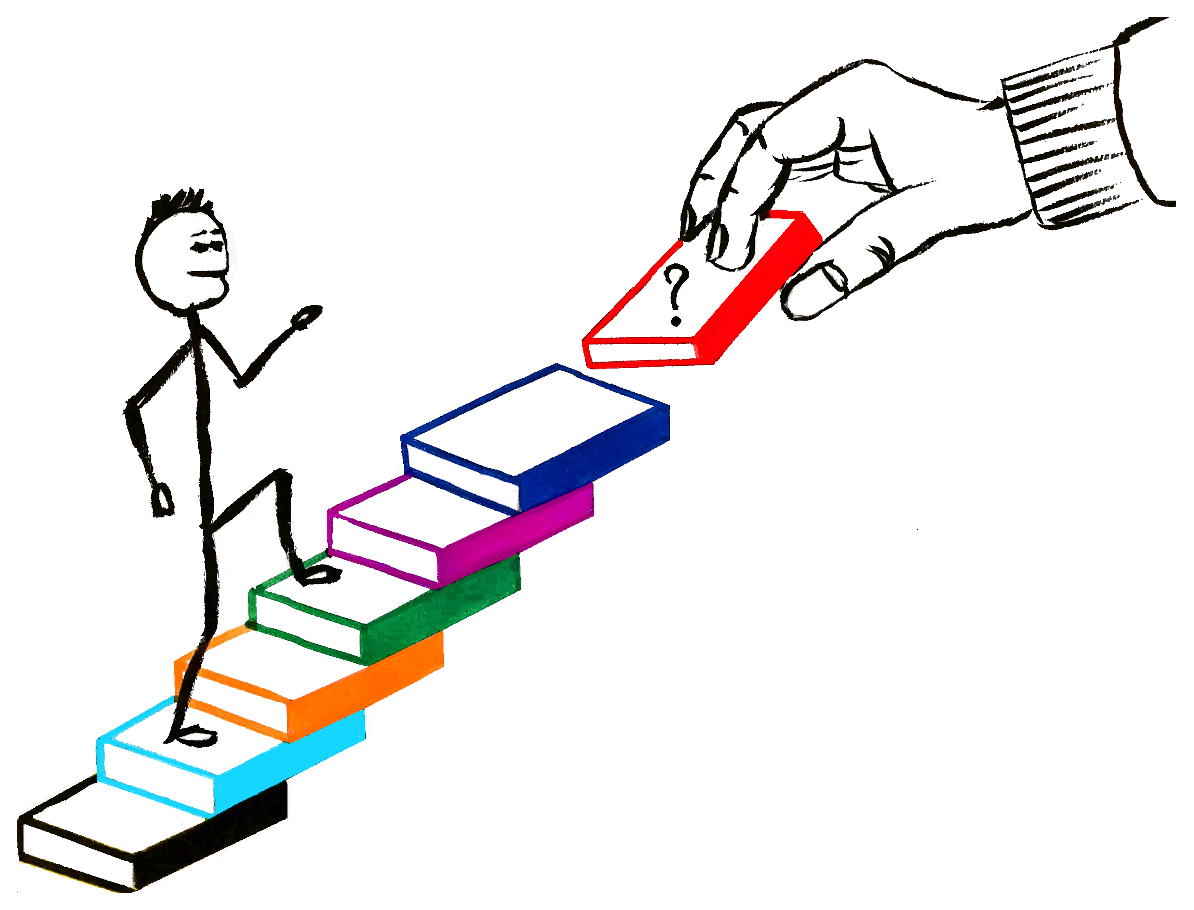
\includegraphics[height=6cm]{escaliers_Nath}}
      \rput[lb](8,1){\parbox{6.5cm}{\it Un escalier compte moins de 100 marches. \\
   Si on le monte 3 par 3, 4 par 4, ou encore 5 par 5, à chaque fois on arrive exactement sur la dernière marche.}}
         \end{pspicture}
\partie[les questions]
   \begin{enumerate}
      \item Combien y a-t-il de marches à cet escalier ?
      \item Arriverait-on exactement sur la dernière marche de cet escalier si on le montait :
      \begin{enumerate}
         \item en sautant 6 marches à la fois ?
         \item en sautant 8 marches à la fois ?
         \item en sautant 5 marches, puis 7, à nouveau 5, puis 7, et ainsi de suite ?
         \item en sautant 3 marches, puis 4, à nouveau 3, puis 4, et ainsi de suite ? et en sautant d'abord 4 marches ?
      \end{enumerate}
   \end{enumerate}
\partie[la narration de recherche]
 

%\themaG
\graphicspath{{../../S12_Symetrie_centrale/Images/}}

\chapter{La symétrie centrale}
\label{S12}


%%%%%%%%%%%%%%%%%%%%%%%%%%%%%%%%%%%%%%%%%%
%%%%%%%%%%%%%%%%%%%%%%%%%%%%%%%%%%%%%%%%%%
\begin{prerequis}
   \begin{itemize}
      \item[\com] Comprendre l'effet d'une symétrie (axiale et centrale) sur une figure.
   \end{itemize}
\end{prerequis}

\vfill

\begin{debat}[Débat : les pavages] 
   Un {\bf pavage du plan} est un ensemble de portions du plan qui, lorsqu'on les met les unes à côté des autres, forment le plan tout entier, sans recouvrement. Par exemple, lorsque l'on pose du carrelage, on effectue un pavage de la pièce. Ce carrelage peut être de forme carrée, rectangulaire, hexagonale\dots
   \begin{center}
      \begin{pspicture}(-3,-3)(3,3)
         \psset{dimen=middle}
         \pstVerb{/aP 3 sqrt 3 div 1 mul def
         /MajorAxis 2 aP mul 3 sqrt mul def
         /LengthSideHexagon aP 3 sqrt 1 sub mul def
         /HeightHexagon 3 3 sqrt sub 2 div aP mul def
         % pentagone 0
         /A0 { 0 aP 2 div 1 3 sqrt add mul HeightHexagon add} def
         /B0 {aP 2 div 3 sqrt mul neg aP 2 div 3 sqrt mul HeightHexagon add} def
         /C0 {aP 2 div 3 sqrt 1 sub mul neg HeightHexagon} def
         /D0 {aP 2 div 3 sqrt 1 sub mul HeightHexagon} def
         /E0 {aP 2 div 3 sqrt mul     aP 2 div 3 sqrt mul HeightHexagon add} def
         %%%% hexagone %%%%
         /H0 {LengthSideHexagon 0} def
         /H1 {LengthSideHexagon 60 cos mul LengthSideHexagon 60 sin mul} def
         /H2 {LengthSideHexagon 120 cos mul LengthSideHexagon 120 sin mul} def
         /H3 {LengthSideHexagon neg 0} def
         /H4 {LengthSideHexagon 240 cos mul LengthSideHexagon 240 sin mul} def
         /H5 {LengthSideHexagon 300 cos mul LengthSideHexagon 300 sin mul} def
         %%%% sommets grand hexagone
         /HX0 {0 2 aP mul} def
         /HX1 {aP 3 sqrt neg mul aP} def
         /HX2 {aP 3 sqrt mul neg aP neg} def
         /HX3 {0 -2 aP mul} def
         /HX4 {aP 3 sqrt mul aP neg} def
         /HX5  {aP 3 sqrt mul aP} def
         }%
         \def\pentagone{\pspolygon(!A0)(!B0)(!C0)(!D0)(!E0)}%
         \def\hexagone{\pspolygon[linecolor=B1](!H0)(!H1)(!H2)(!H3)(!H4)(!H5)}%
         \def\motifA{\multido{\i=0+60}{6}{\rput{\i}{\pentagone}}\hexagone}
         \motifA\rput(!MajorAxis 0){\motifA}
         \motifA\rput(!MajorAxis neg 0){\motifA}
         \rput(!MajorAxis 2 div aP 3 mul){\motifA}
         \rput(!MajorAxis 2 div aP -3 mul){\motifA}
         \rput(!MajorAxis -2 div aP 3 mul){\motifA}
         \rput(!MajorAxis -2 div aP -3 mul){\motifA}
      \end{pspicture}
   \end{center}
   \bigskip
   \begin{cadre}[B2][F4]
      \begin{center}
         Vidéo : \href{http://therese.eveilleau.pagesperso-orange.fr/pages/truc_mat/textes/pavages.htm}{\bf Pavages interactifs}, site Internet {\it Mathématiques magiques} de {\it Thérèse Eveilleau}.
      \end{center}
   \end{cadre}
\end{debat}

\vfill

\textcolor{PartieGeometrie}{\sffamily\bfseries Cahier de compétences} : chapitre 7, exercices 1 à 33.


%%%%%%%%%%%%%%%%%%%%%%%%%%%%%%%%%%
%%%%%%%%%%%%%%%%%%%%%%%%%%%%%%%%%
\activites

\begin{activite}[Le bonhomme inversé]
   {\bf Objectifs :} transformer une figure par symétrie axiale ; observer l'effet de deux symétries axiales. \\ 
   \begin{QCM}
      Construire sur le quadrillage ci-dessous les bonhommes demandés.
      \begin{enumerate}
         \item Construire en vert le symétrique du bonhomme par rapport à la droite $(d)$. 
         \item Construire en rouge le symétrique du bonhomme vert par rapport à
la droite $(\Delta)$.
         \item Reproduire sur du papier calque le bonhomme noir et le point $O$.
         \item En s'aidant du calque, sans le plier, trouver comment passer du bonhomme noir au bonhomme rouge.
         \item Sans utiliser les bonhommes noir et rouge ni les droites $(d)$ et $(\Delta)$, construire en bleu l'image du bonhomme vert par la symétrie centrale de centre $O$. \\
      \end{enumerate}
      \begin{center}
      {\psset{unit=0.65}
         \begin{pspicture}(-11,-11)(11,11)
            \psgrid[subgriddiv=0,gridlabels=0,gridcolor=gray](-11,-11)(11,11)
            \psline[linewidth=0.5mm](-11,0)(11,0)
            \psline[linewidth=0.5mm](0,-11)(0,11)
            \rput(0.5,-0.5){$O$}
            \rput(10.5,0.5){$(\Delta)$}
            \rput(0.7,10.5){$(d)$}
            \psset{linewidth=1mm}
            \psline(2,1)(3,1)(5,4)(7,1)(8,1)
            \psline(5,4)(5,7)
            \psframe(4,7)(6,9)
            \psline(3,5)(7,6)
            \psdots(3,5)(7,6)(4.5,8.5)
            \psline(5.25,8.5)(5.75,8.5)
            \psarc(5,8){0.5}{180}{0}
            \psline(3,9)(7,9)
            \psarc(5,9){1}{0}{180}
         \end{pspicture}}
      \end{center}
  \end{QCM}
  \vfill\hfill{\it\footnotesize Source : \href{https://irem.univ-lille1.fr/IMG/pdf/fiche_eleve_symetrie.pdf}{À la découverte de la symétrie centrale, Nathalie Bernard, IREM de Lille.}}
\end{activite}


%%%%%%%%%%%%%%%%%%%%%%%%%%%%%%%%%%%%
%%%%%%%%%%%%%%%%%%%%%%%%%%%%%%%%%%%%
\cours 

\section{La symétrie centrale} %%%%%%

\begin{definition}
   Le point $M'$ est l'image du point $M$ par la \textbf{symétrie de centre $O$} lorsque le point $O$ est le milieu du segment $[MM']$.
\end{definition}

\medskip

\begin{methode}[Construire le symétrique d'un point par symétrie centrale]
   Pour construire le symétrique d'un point $M$ par la symétrie centrale de centre $O$ :
   \begin{itemize}
      \item tracer la demi-droite $[MO)$ ;
      \item reporter la longueur $MO$ de l'autre côté du point $O$ ;
      \item placer le point $M'$ symétrique de $M$ par rapport à $O$.
   \end{itemize}
   \exercice
      Tracer le point $M'$, symétrique du point $M$ par rapport à $O$. \\
      \small
      \begin{pspicture}(0,-0.2)(4,1.7)
         \pstGeonode[PosAngle=-90,PointSymbol=+](0.5,0.5){M}(2,1){O}
         \pstLineAB[linecolor=A1]{M}{O}
      \end{pspicture}
   \correction
      \begin{pspicture}(0,-0.2)(4,2.2)
         \pstGeonode[PosAngle=-90,PointSymbol=+](0.5,0.5){M}(2,1){O}
         \pstLineAB[linecolor=A1]{M}{O}
         \pstGeonode[PointSymbol=none,PointName=none](4,1.67){N}
         \pstLineAB[linecolor=B1]{O}{N}
      \end{pspicture}
      \begin{pspicture}(0,-0.2)(4,2.2)
         \pstGeonode[PosAngle=-90,PointSymbol=+](0.5,0.5){M}(2,1){O}
         \pstGeonode[PointSymbol=none,PointName=none](4,1.67){N}
         \pstSymO[CodeFig=true,CodeFigColor=black,PosAngle=-90,SegmentSymbol=pstslashh]{O}{M}[M']
         \pstLineAB[linecolor=A1]{M}{O}
         \pstLineAB[linecolor=B1]{O}{N}
      \end{pspicture}
\end{methode}

\begin{remarque}
   transformer une figure par symétrie centrale de centre $O$ revient à lui faire faire un demi-tour autour de ce point.
\end{remarque}

\begin{minipage}{7cm}
   Pour tracer la figure symétrique d'une figure par la symétrie centrale de centre $O$, il faut construire le symétrique de chacun des points qui la compose.
\end{minipage}
\quad
\begin{minipage}{8cm}
   {\psset{unit=0.8}
   \begin{pspicture}(-5,-0)(4,3.5)
      \pstGeonode[PosAngle=-90](0,1.5){O}
      \pstTriangle(1,0){A}(4,0){B}(2,2){C}
      \pstSymO[CodeFig=true, CodeFigColor=A1, PosAngle={40,170,-90}]{O}{A, B, C}[A', B', C']
      \pstLineAB[linecolor=B1]{A'}{B'}
      \pstLineAB[linecolor=B1]{C'}{B'}
      \pstLineAB[linecolor=B1]{A'}{C'}
   \end{pspicture}}
\end{minipage}


\section{Centre de symétrie} %%%%%%

\begin{definition}
   Si une figure $\cal F$ est transformée en elle-même par la symétrie centrale de centre O, alors O est le \textbf{centre de symétrie} de la figure $\cal F$.
\end{definition}

\begin{exemple*1}
   Si une figure possède un centre de symétrie, alors il est unique.
   {\psset{unit=0.75}
   \begin{multicols}{3}
      \begin{center}
         \begin{pspicture}(-2.5,-0.5)(2.5,2.3)
            \pstGeonode[PointName=none,PointSymbol=none,CurveType=polygon](-1.156,0){A}(1.156,0){B}(0,2){C}
            \pstGeonode[PointName=none,PointSymbol=none,CurveType=polygon,linecolor=B1](0,-0.5){D}(0,2.5){E}
            \psline[linecolor=B1](-1.156,0)(2;50)
            \psline[linecolor=B1](1.156,0)(2;130)
         \end{pspicture}
   
         3 axes de symétrie \\
         0 centre de symétrie
         \begin{pspicture}(-2.5,-0.5)(2.5,2.3)
            \pscircle(0,1){1}
            \psset{linecolor=B1}
            \psline(-1.5,1)(1.5,1)
            \psline(0,-0.5)(0,2.5)
            \psline(-1.5,-0.5)(1.5,2.5)
            \psline(-1.5,2.5)(1.5,-0.5)
            \psline(-0.5,-0.5)(0.5,2.5)
            \psline(-0.5,2.5)(0.5,-0.5)
            \psline(-1.5,0)(1.5,2)
            \psline(-1.5,0.5)(1.5,1.5)
            \psline(-1.5,2)(1.5,0)
            \psline(-1.5,1.5)(1.5,0.5)
            \psdot[linecolor=A1,linewidth=1mm](0,1)  
         \end{pspicture}
   
         $\infty$ axes de symétrie \\
         1 centre de symétrie  
      \end{center}
   
      \begin{pspicture}(-2.5,-0.5)(2.5,2.3)
         \pspolygon(-1.5,0)(1.5,0)(1.5,2)(-1.5,2)
         \psset{linecolor=B1}
         \psline(-2,1)(2,1)
         \psline(0,-0.5)(0,2.5)
         \psdot[linecolor=A1,linewidth=1mm](0,1)  
      \end{pspicture}
   
      \quad 2 axes de symétrie
      
      \quad 1 centre de symétrie
   \end{multicols}}
\vspace*{-5mm}
\end{exemple*1}


%%%%%%%%%%%%%%%%%%%%%%%%%%%%%%%%%%%%%%%%%%
%%%%%%%%%%%%%%%%%%%%%%%%%%%%%%%%%%%%%%%%%%
\exercicesbase

\begin{colonne*exercice}

\serie{Construction de symétriques}

\begin{exercice} %1
   Construire les points $I', K', R'$ et $A'$ symétriques respectifs de $I, K, R$ et $A$ par rapport au point $M$.
   \begin{center}
      {\psset{unit=0.6}
      \begin{pspicture}(12,8)
        \small
        \psgrid[subgriddiv=0,gridlabels=0,gridcolor=darkgray](0,0)(12,8)
         \pstGeonode[,PosAngle=45](2,2){R}(3,5){I}(8,5){K}(6,2){A}(6,4){M}
      \end{pspicture}}
   \end{center} 
\end{exercice}

\begin{corrige}
   \ \\ [-3mm]
   {\psset{unit=0.6}
   \begin{pspicture}(0,-1)(12,8)
     \small
     \psgrid[subgriddiv=0,gridlabels=0,gridcolor=darkgray](0,0)(12,8)
         \pstGeonode[,PosAngle=45](2,2){R}(3,5){I}(8,5){K}(6,2){A}(6,4){M}
        \blue
        \pstGeonode[PosAngle=45,linecolor=blue](10,6){R'}(9,3){I'}(4,3){K'}(6,6){A'}
   \end{pspicture}}
\end{corrige}


\begin{exercice} %2
   Sur la figure ci-dessous, $DEFG$ est un rectangle de centre $L$. Les points $R, C, N$ et $S$ sont les milieux respectifs des côtés $[DE], [EF], [FG]$ et $[GD]$.
   \begin{center}
      {\small
      \psset{xunit=0.5}
      \begin{pspicture}(-0.5,-0.3)(8.5,4.5)
         \psframe(0,0)(8,4)
         \pspolygon(4,0)(8,2)(4,4)(0,2)
         \psline(0,4)(8,0)
         \psline(0,0)(8,4)
         \psline(0,2)(8,2)
         \psline(4,0)(4,4)
\pstGeonode[PosAngle={-135,-90,-45,-90,-90,180,70,0,90,90,135,90,45},PointSymbol=none](0,0){E}(4,0){C}(8,0){F}(2,1){Y}(6,1){P}(0,2){R}(4,2){L}(8,2){N}(2,3){H}(6,3){K}(0,4){D}(4,4){S}(8,4){G}
      \end{pspicture}}
   \end{center}
   \begin{enumerate}
      \item Colorier en jaune le triangle $DHS$.
      \item Colorier en rouge le symétrique du triangle $DHS$ par rapport à $(RN)$.
      \item Colorier en orange le symétrique du triangle $DHS$ par rapport à $(SC)$
      \item Colorier en bleu le symétrique du triangle $DHS$ par rapport à $H$.
      \item Colorier en vert le symétrique du triangle $DHS$ par rapport à $L$.
   \end{enumerate}
\end{exercice}

\begin{corrige}
   \ \\ [-6mm]
   {\psset{xunit=0.45,yunit=0.9}
   \small
   \begin{pspicture}(-4,-1)(8.5,4.7)
      \pspolygon[fillstyle=solid,fillcolor=yellow](0,4)(2,3)(4,4)
      \pspolygon[fillstyle=solid,fillcolor=red](0,0)(2,1)(4,0)
      \pspolygon[fillstyle=solid,fillcolor=orange](8,4)(6,3)(4,4)
      \pspolygon[fillstyle=solid,fillcolor=blue](0,2)(4,2)(2,3)
      \pspolygon[fillstyle=solid,fillcolor=green](4,0)(8,0)(6,1)
      \psframe(0,0)(8,4)
      \pspolygon(4,0)(8,2)(4,4)(0,2)
      \psline(0,4)(8,0)
      \psline(0,0)(8,4)
      \psline(0,2)(8,2)
      \psline(4,0)(4,4)
      \pstGeonode[PosAngle={-135,-90,-45,-90,-90,180,70,0,90,90,135,90,45},PointSymbol=none](0,0){E}(4,0){C}(8,0){F}(2,1){Y}(6,1){P}(0,2){R}(4,2){L}(8,2){N}(2,3){H}(6,3){K}(0,4){D}(4,4){S}(8,4){G}  
   \end{pspicture}}
\end{corrige}


\begin{exercice} %3
   Dans chaque cas, reproduire la lettre sur le cahier et construire son symétrique par rapport au point $B$.
   \begin{center}
      {\small
      \psset{unit=0.6,subgriddiv=0,gridlabels=0,gridcolor=darkgray}
      \begin{pspicture}(2.3,3)
        \psgrid(0,0)(2,3)
        \pstGeonode[PosAngle=-45](1,1){B}
        \psset{linewidth=0.6mm}
        \psline(0,1)(0,3)(1,3)(1,1)
        \psline(0,2)(1,2)
     \end{pspicture}
     \begin{pspicture}(2.3,3)
        \psgrid(0,0)(2,3)
        \pstGeonode[PosAngle=-135](1,1){B}
        \psset{linewidth=0.6mm}
        \psline(2,1)(1,1)(1,3)(2,3)
     \end{pspicture}
     \begin{pspicture}(2.3,3)
        \psgrid(0,0)(2,3)
        \pstGeonode[PosAngle=45](1,0){B}
        \psset{linewidth=0.6mm}
        \psline(1,1)(0,1)(0,3)(1,3)
        \psline(0,2)(1,2)
     \end{pspicture}
     \begin{pspicture}(2.3,3)
        \psgrid(0,0)(2,3)
        \pstGeonode[PosAngle=-135](2,1){B}
        \psset{linewidth=0.6mm}
        \psline(0,1)(0,3)
        \psline(0,2)(1,2)
        \psline(1,1)(1,3)
     \end{pspicture}
     \begin{pspicture}(2.3,3)
        \psgrid(0,0)(2,3)
        \pstGeonode[PosAngle=-135](1,3){B}
        \psset{linewidth=0.6mm}
        \psline(1,2)(1,0)(2,0)
     \end{pspicture}}
   \end{center}
\end{exercice} 

\begin{corrige}
   \ \\ [-2mm]
   {\psset{unit=0.6,subgriddiv=0,gridlabels=0,gridcolor=darkgray}
   \begin{pspicture}(-1,-3)(2.5,4)
      \psgrid(-1,-2)(2,4)
      \pstGeonode[PosAngle=-45](1,1){B}
      \psset{linewidth=0.6mm}
      \psline(0,1)(0,3)(1,3)(1,1)
      \psline(0,2)(1,2)
      \psset{linecolor=blue}
      \psline(1,0)(2,0)  
      \psline(1,1)(1,-1)(2,-1)(2,1)
   \end{pspicture}
   \begin{pspicture}(-1,-3)(3.5,4)
      \psgrid(-1,-2)(3,4)
      \pstGeonode[PosAngle=-135](1,1){B}
      \psset{linewidth=0.6mm}
      \psline(2,1)(1,1)(1,3)(2,3)
      \psset{linecolor=blue}
      \psline(0,1)(1,1)(1,-1)(0,-1)
   \end{pspicture}
   \begin{pspicture}(-1,-4)(3,4)
      \psgrid(-1,-4)(3,4)
      \pstGeonode[PosAngle=45](1,0){B}
      \psset{linewidth=0.6mm}
      \psline(1,1)(0,1)(0,3)(1,3)
      \psline(0,2)(1,2)
      \psset{linecolor=blue}
      \psline(1,-1)(2,-1)(2,-3)(1,-3)
      \psline(1,-2)(2,-2)
   \end{pspicture}
     
   \begin{pspicture}(-1,-3)(6,4)
      \psgrid(-1,-3)(5,4)
      \pstGeonode[PosAngle=-135](2,1){B}
      \psset{linewidth=0.6mm}
      \psline(0,1)(0,3)
      \psline(0,2)(1,2)
      \psline(1,1)(1,3)
      \psset{linecolor=blue}
      \psline(3,0)(3,-2)
      \psline(4,0)(4,-2)
      \psline(3,-1)(4,-1)
  \end{pspicture}
  \begin{pspicture}(-1,-1)(4,7.5)
      \psgrid(-1,-1)(3,7)
      \pstGeonode[PosAngle=-135](1,3){B}
      \psset{linewidth=0.6mm}
      \psline(1,2)(1,0)(2,0)
      \psset{linecolor=blue}
      \psline(1,4)(1,6)(2,6)
   \end{pspicture}}
\end{corrige}  


\begin{exercice} %4
   Colorier le minimum de cases pour que chacune des figures ci-dessous admette le point $O$ pour centre de symétrie.
   {\psset{unit=0.45,subgriddiv=0,gridlabels=0,gridcolor=darkgray}
   \begin{center}
      \begin{pspicture}(0,0)(8,8)
        \psgrid[subgriddiv=0,gridlabels=0](0,0)(8,8)
        \pstGeonode[PosAngle=-45](4,4){O}
        \psset{fillstyle=solid,fillcolor=black!80}
        \psframe(0,0)(1,1)
        \rput(5,7){\psframe(0,0)(1,1)}
        \rput(6,3){\psframe(0,0)(1,1)}
        \rput(3,2){\psframe(0,0)(1,1)}
        \psset{fillcolor=gray!50}
        \rput(1,5){\psframe(0,0)(1,1)}
        \rput(4,4){\psframe(0,0)(1,1)}
        \rput(5,2){\psframe(0,0)(1,1)}
        \rput(3,7){\psframe(0,0)(1,1)}   
     \end{pspicture}
     \;
     \begin{pspicture}(0,0)(8,8)        
        \psset{fillstyle=solid,fillcolor=black!80}
        \psframe(0,0)(1,3)
        \rput(6,3){\psframe(0,0)(1,2)}
        \rput(2,2){\psframe(0,0)(2,1)}
        \rput(1,5){\psframe(0,0)(1,2)}
        \rput(4,4){\psframe(0,0)(3,1)}
        \rput(5,2){\psframe(0,0)(1,2)}
        \rput(3,7){\psframe(0,0)(4,1)}
        \psgrid[subgriddiv=0,gridlabels=0](0,0)(8,8)
        \pstGeonode[PosAngle=-45](4,4){O}
     \end{pspicture}
   \end{center}}
\end{exercice} 

\begin{corrige}
   \ \\ [-3mm]
   {\psset{unit=0.45,subgriddiv=0,gridlabels=0,gridcolor=darkgray}
   \begin{pspicture}(0,0)(8,8)
     \psgrid[subgriddiv=0,gridlabels=0](0,0)(8,8)
     \pstGeonode[PosAngle=-45](4,4){O}
     \psset{fillstyle=solid,fillcolor=black!80}
     \psframe(0,0)(1,1)
     \rput(5,7){\psframe(0,0)(1,1)}
     \rput(6,3){\psframe(0,0)(1,1)}
     \rput(3,2){\psframe(0,0)(1,1)}
     \rput(4,5){\psframe(0,0)(1,1)}
     \rput(2,0){\psframe(0,0)(1,1)}
     \rput(1,4){\psframe(0,0)(1,1)}
     \rput(7,7){\psframe(0,0)(1,1)}
     \psset{fillcolor=gray!50}
     \rput(1,5){\psframe(0,0)(1,1)}
     \rput(4,4){\psframe(0,0)(1,1)}
     \rput(5,2){\psframe(0,0)(1,1)}
     \rput(3,7){\psframe(0,0)(1,1)}  
     \rput(3,3){\psframe(0,0)(1,1)}
     \rput(6,2){\psframe(0,0)(1,1)}
     \rput(4,0){\psframe(0,0)(1,1)}
     \rput(2,5){\psframe(0,0)(1,1)}
  \end{pspicture}
  \;
  \begin{pspicture}(0,0)(8,8)        
     \psset{fillstyle=solid,fillcolor=black!80}
     \pspolygon(0,0)(5,0)(5,1)(1,1)(1,3)(0,3)
     \pspolygon(1,3)(2,3)(2,2)(4,2)(4,4)(3,4)(3,6)(2,6)(2,7)(1,7)
     \pspolygon(3,7)(3,8)(8,8)(8,5)(7,5)(7,7)
     \pspolygon(4,4)(4,6)(6,6)(6,5)(7,5)(7,1)(6,1)(6,2)(5,2)(5,4)
     \psgrid[subgriddiv=0,gridlabels=0](0,0)(8,8)
     \pstGeonode[PosAngle=-45](4,4){O}
  \end{pspicture}}
\end{corrige}


\begin{exercice} %5
   Tracer la figure symétrique de toutes les figures par rapport au point $O$.
   {\psset{unit=0.45cm}
   \begin{center}
      \begin{pspicture}(18,18)
         \psgrid[subgriddiv=1,griddots=10,gridlabels=0,gridcolor=darkgray]
         \psdot(9,9)
         \psset{linewidth=1.5pt}
         \pspolygon(1,8)(2,9)(3,8)(5,8)(6,9)(5,9)(6,10)(5,11)(3,11)(2,10)(1,11)
         \pspolygon(1,13)(3,17)(7,17)(9,13)
         \pscircle(5,15){1}
         \psdot(5,10)
         \psline(7,13)(7,17)
         \psline(3,13)(3,17)
         \pspolygon(12,14)(15,14)(16,15)(12,15)
         \psline(14,15)(14,18)(13,16)(14,16)
      \end{pspicture}
   \end{center}}
\end{exercice}

\begin{corrige}
   \ \\ [-3mm]
   {\psset{unit=0.41cm}
   \begin{pspicture}(18,18)
      \psgrid[subgriddiv=1,griddots=10,gridlabels=0,gridcolor=gray]
      \psdot(9,9)
      \psset{linewidth=1.5pt}
      \pspolygon(1,8)(2,9)(3,8)(5,8)(6,9)(5,9)(6,10)(5,11)(3,11)(2,10)(1,11)
      \pspolygon(1,13)(3,17)(7,17)(9,13)
      \pscircle(5,15){1}
      \psdot(5,10)
      \psline(7,13)(7,17)
      \psline(3,13)(3,17)
      \pspolygon(12,14)(15,14)(16,15)(12,15)
      \psline(14,15)(14,18)(13,16)(14,16)
      \psset{linecolor=blue}
      \pspolygon(17,10)(16,9)(15,10)(13,10)(12,9)(13,9)(12,8)(13,7)(15,7)(16,8)(17,7)
      \pspolygon(17,5)(15,1)(11,1)(9,5)
      \pscircle(13,3){1}
      \psdot(13,8)
      \psline(11,5)(11,1)
      \psline(15,5)(15,1)
      \pspolygon(6,4)(3,4)(2,3)(6,3)
      \psline(4,3)(4,0,)(5,2)(4,2)
      \psset{linecolor=blue}
   \end{pspicture}}
\end{corrige}

\end{colonne*exercice}

\begin{exercice} %6
   Pour chacun de ces panneaux de signalisation, tracer le ou les axes et/ou centre de symétrie.
   \begin{center}
      {\psset{unit=0.8}
      \begin{pspicture}(-0.9,-1)(1.3,1) %1
         \pscircle[linewidth=0.3,linecolor=red](0,0){0.85}
      \end{pspicture} 
      \begin{pspicture}(-1,-1)(1.3,1) %2
         \psframe[framearc=0.15](-1,-1)(1,1)
         \psframe[framearc=0.05,fillstyle=solid,fillcolor=blue,linecolor=blue](-0.9,-0.9)(0.9,0.9)
         \psframe[fillstyle=solid,fillcolor=white,linecolor=white](-0.15,-0.8)(0.15,0.3)
         \psframe[fillstyle=solid,fillcolor=white,linecolor=white](-0.4,0.3)(0.4,0.8)
         \psframe[fillstyle=solid,fillcolor=red,linecolor=red](-0.35,0.35)(0.35,0.75)
      \end{pspicture}
      \begin{pspicture}(-1,-1)(1.3,1) %3
         \pscircle[linewidth=0.3,linecolor=red](0,0){0.85}
         \psline[linewidth=0.2,linecolor=black](0.25,-0.55)(0.25,0.25)
         \psarc[linewidth=0.2,linecolor=black](0,0.25){0.25}{0}{180}
         \psline[linewidth=0.2,linecolor=black,arrowinset=0,arrowlength=0.5]{->}(-0.25,0.25)(-0.25,-0.4)
         \psline[linewidth=0.2,linecolor=red](1;135)(1;-45)
      \end{pspicture}   
      \begin{pspicture}(-1,-1)(1.3,1) %4
         \pspolygon[linearc=0.05,fillstyle=solid,fillcolor=white](0,-1)(1,0)(0,1)(-1,0)
         \pspolygon[linearc=0.05,fillstyle=solid,fillcolor=yellow](0,-0.68)(0.68,0)(0,0.68)(-0.68,0)
         \psline[linewidth=0.3,linecolor=black](0.7;-135)(0.7;45)
      \end{pspicture}
      \begin{pspicture}(-1,-1)(1.3,1) %5
         \pscircle[fillstyle=solid,fillcolor=blue,linecolor=blue](0,0){1}
         \psline[linewidth=0.2,linecolor=white](0,-0.9)(0,0.05)
         \psarc[linewidth=0.2,linecolor=white](0.4,0){0.4}{90}{180}
         \psline[linewidth=0.2,linecolor=white,arrowlength=0.8]{->}(0.35,0.4)(0.8,0.4)
         \psarc[linewidth=0.2,linecolor=white](-0.4,0){0.4}{0}{90}
         \psline[linewidth=0.2,linecolor=white,arrowlength=0.8]{->}(-0.35,0.4)(-0.8,0.4)
      \end{pspicture}
      \begin{pspicture}(-1,-1)(1.3,1) %6
         \psframe[framearc=0.15](-1,-1)(1,1)
         \psframe[linewidth=0.2,linecolor=blue](-0.8,-0.8)(0.8,0.8)
         \psline[linewidth=0.4,linecolor=red](0,-0.65)(0,0.65)
         \psline[linewidth=0.4,linecolor=red](-0.65,0)(0.65,0)
      \end{pspicture}
      \begin{pspicture}(-1,-1)(1.3,1) %7
         \pspolygon[linearc=0.05,fillstyle=solid,fillcolor=white](0,-1)(1,0)(0,1)(-1,0)
         \pspolygon[linearc=0.05,fillstyle=solid,fillcolor=yellow](0,-0.68)(0.68,0)(0,0.68)(-0.68,0)
      \end{pspicture}
      \begin{pspicture}(-1,-1)(1.3,1) %8
         \pscircle[fillstyle=solid,fillcolor=red,linecolor=red](0,0){1}
         \pscircle[fillstyle=solid,fillcolor=blue,linecolor=blue](0,0){0.7}
         \psline[linewidth=0.2,linecolor=red](1;-135)(1;45)
         \psline[linewidth=0.2,linecolor=red](1;135)(1;-45)
      \end{pspicture}
      \begin{pspicture}(-1,-1)(0.9,1) %9
         \psframe[framearc=0.15](-1,-1)(1,1)
         \psframe[framearc=0.05,fillstyle=solid,fillcolor=blue,linecolor=blue](-0.9,-0.9)(0.9,0.9)
         \pspolygon[linewidth=0.15,linecolor=orange](0.55;30)(0.55;90)(0.55;150)(0.55;210)(0.55;270)(0.55;330)
      \end{pspicture}}
   \end{center}
\end{exercice}

\begin{corrige}
   \ \\ [-3mm]
   {\psset{unit=0.8}
      \begin{pspicture}(-1.5,-2)(2,1) %1
         \pscircle[linewidth=0.3,linecolor=red](0,0){0.85}
         \psset{linecolor=gray,linewidth=0.05}
         \psline(1.3;0)(1.3;180)
         \psline(1.3;30)(1.3;210)
         \psline(1.3;45)(1.3;225)
         \psline(1.3;90)(1.3;270)
         \psline(1.3;120)(1.3;300)
         \psline(1.3;150)(1.3;330)
         \psline(1.3;60)(1.3;240)
         \psdot[linecolor=green,linewidth=0.1](0,0)
      \end{pspicture} 
      \begin{pspicture}(-1,-2)(2,1) %2
         \psframe[framearc=0.15](-1,-1)(1,1)
         \psframe[framearc=0.05,fillstyle=solid,fillcolor=blue,linecolor=blue](-0.9,-0.9)(0.9,0.9)
         \psframe[fillstyle=solid,fillcolor=white,linecolor=white](-0.15,-0.8)(0.15,0.3)
         \psframe[fillstyle=solid,fillcolor=white,linecolor=white](-0.4,0.3)(0.4,0.8)
         \psframe[fillstyle=solid,fillcolor=red,linecolor=red](-0.35,0.35)(0.35,0.75)
         \psset{linecolor=gray}
         \psline(1.3;90)(1.3;270)
      \end{pspicture}
      \begin{pspicture}(-1,-2)(1,1) %3
         \pscircle[linewidth=0.3,linecolor=red](0,0){0.85}
         \psline[linewidth=0.2,linecolor=black](0.25,-0.55)(0.25,0.25)
         \psarc[linewidth=0.2,linecolor=black](0,0.25){0.25}{0}{180}
         \psline[linewidth=0.2,linecolor=black,arrowinset=0,arrowlength=0.5]{->}(-0.25,0.25)(-0.25,-0.4)
         \psline[linewidth=0.2,linecolor=red](1;135)(1;-45) 
      \end{pspicture}   
      
      \begin{pspicture}(-1.5,-2)(2,1) %4
         \pspolygon[linearc=0.05,fillstyle=solid,fillcolor=white](0,-1)(1,0)(0,1)(-1,0)
         \pspolygon[linearc=0.05,fillstyle=solid,fillcolor=yellow](0,-0.68)(0.68,0)(0,0.68)(-0.68,0)
         \psline[linewidth=0.3,linecolor=black](0.7;-135)(0.7;45)
         \psset{linecolor=gray}
         \psline(1.3;45)(1.3;225)
         \psline(1.3;-45)(1.3;-225)
         \psdot[linecolor=green,linewidth=0.1](0,0)
      \end{pspicture}
      \begin{pspicture}(-1,-2)(2,1) %5
         \pscircle[fillstyle=solid,fillcolor=blue,linecolor=blue](0,0){1}
         \psline[linewidth=0.2,linecolor=white](0,-0.9)(0,0.05)
         \psarc[linewidth=0.2,linecolor=white](0.4,0){0.4}{90}{180}
         \psline[linewidth=0.2,linecolor=white,arrowlength=0.8]{->}(0.35,0.4)(0.8,0.4)
         \psarc[linewidth=0.2,linecolor=white](-0.4,0){0.4}{0}{90}
         \psline[linewidth=0.2,linecolor=white,arrowlength=0.8]{->}(-0.35,0.4)(-0.8,0.4)
         \psset{linecolor=gray}
         \psline(1.3;90)(1.3;270)
      \end{pspicture}
      \begin{pspicture}(-1,-2)(1,1) %6
         \psframe[framearc=0.15](-1,-1)(1,1)
         \psframe[linewidth=0.2,linecolor=blue](-0.8,-0.8)(0.8,0.8)
         \psline[linewidth=0.4,linecolor=red](0,-0.65)(0,0.65)
         \psline[linewidth=0.4,linecolor=red](-0.65,0)(0.65,0)
         \psset{linecolor=gray}
         \psline(1.3;0)(1.3;180)
         \psline(1.5;45)(1.5;225)
         \psline(1.3;90)(1.3;270)
         \psline(1.5;135)(1.5;315)
         \psdot[linecolor=green,linewidth=0.1](0,0)
      \end{pspicture}
     
      \begin{pspicture}(-1.5,-1)(2,1) %7
         \pspolygon[linearc=0.05,fillstyle=solid,fillcolor=white](0,-1)(1,0)(0,1)(-1,0)
         \pspolygon[linearc=0.05,fillstyle=solid,fillcolor=yellow](0,-0.68)(0.68,0)(0,0.68)(-0.68,0)
         \psset{linecolor=gray}
         \psline(1.3;0)(1.3;180)
         \psline(1.3;45)(1.3;225)
         \psline(1.3;90)(1.3;270)
         \psline(1.3;135)(1.3;315)
         \psdot[linecolor=green,linewidth=0.1](0,0)
      \end{pspicture}
      \begin{pspicture}(-1,-1)(2,1) %8
         \pscircle[fillstyle=solid,fillcolor=red,linecolor=red](0,0){1}
         \pscircle[fillstyle=solid,fillcolor=blue,linecolor=blue](0,0){0.7}
         \psline[linewidth=0.2,linecolor=red](1;-135)(1;45)
         \psline[linewidth=0.2,linecolor=red](1;135)(1;-45)
         \psset{linecolor=gray}
         \psline(1.3;0)(1.3;180)
         \psline(1.3;45)(1.3;225)
         \psline(1.3;90)(1.3;270)
         \psline(1.3;135)(1.3;315)
         \psdot[linecolor=green,linewidth=0.1](0,0)
      \end{pspicture}
      \begin{pspicture}(-1,-1)(1,1) %9
         \psframe[framearc=0.15](-1,-1)(1,1)
         \psframe[framearc=0.05,fillstyle=solid,fillcolor=blue,linecolor=blue](-0.9,-0.9)(0.9,0.9)
         \pspolygon[linewidth=0.15,linecolor=orange](0.55;30)(0.55;90)(0.55;150)(0.55;210)(0.55;270)(0.55;330)
         \psset{linecolor=gray}
         \psline(1.3;0)(1.3;180)
         \psline(1.3;90)(1.3;270)
         \psdot[linecolor=green,linewidth=0.1](0,0)
      \end{pspicture}}
\end{corrige}


%%%%%%%%%%%%%%%%%%%%%%%%%%%%%%%%%%%%%%%%%%
%%%%%%%%%%%%%%%%%%%%%%%%%%%%%%%%%%%%%%%%%%
\Recreation

\enigme[Pavage du plan rectangulaire]
   Un pavage du plan est une portion de plan sur laquelle un motif de base se répète par isométrie (transformation du plan qui conserve les longueurs) tel que les motifs ne se recouvrent pas et ne laissent pas de \og trous \fg. La symétrie centrale est une isométrie. Nous allons composer un pavage à partir d'un motif.
   \begin{center}
      \begin{minipage}{5cm}
         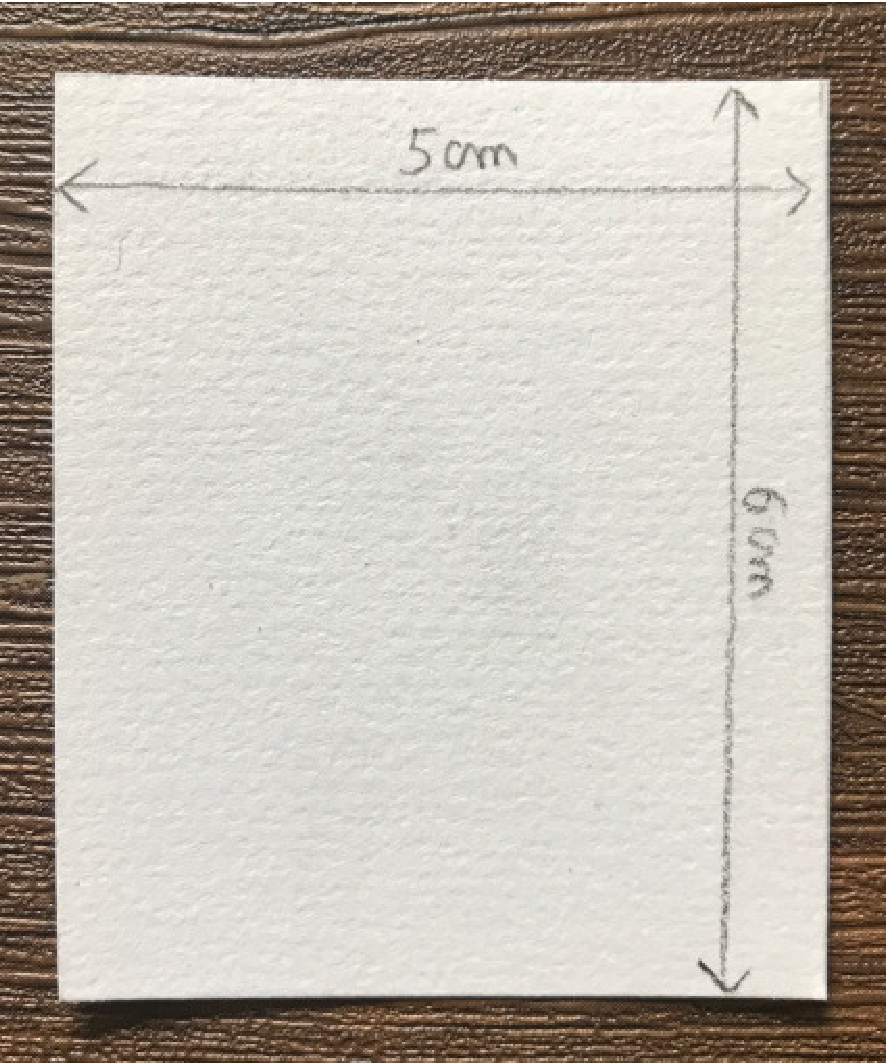
\includegraphics[width=5cm]{pavage1}
      \end{minipage}
      \qquad
      \begin{minipage}{5cm}
         \begin{enumerate}
            \item Découper dans une feuille de papier Canson un rectangle de \ucm{5} sur \ucm{6}. \smallskip
            \item Plier le rectangle en deux dans le sens de la largeur et placer trois petits bouts de scotch sur les trois côtés qui ne sont pas attachés. \smallskip
            \item Dessiner une forme qui ressemble à un poisson en deux morceaux.
         \end{enumerate}
      \end{minipage}
      \qquad
      \begin{minipage}{5cm}
         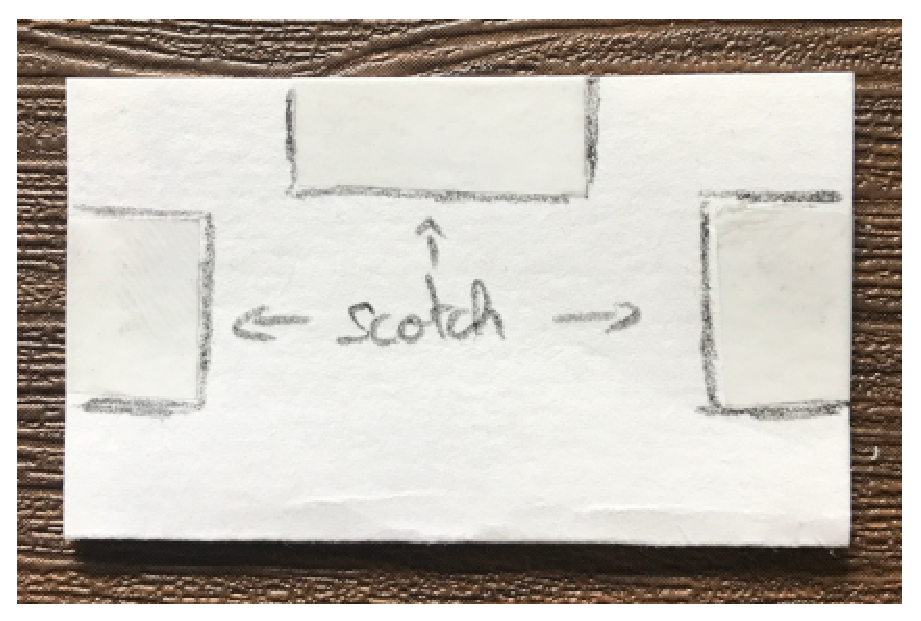
\includegraphics[width=5cm]{pavage2}
         
\includegraphics[width=5cm]{pavage3}
      \end{minipage} \\ \medskip
      \begin{minipage}{7cm}
         \begin{enumerate}
            \setcounter{enumi}{3}
            \item Découper selon les traits en commençant par les coins laissés sans scotch puis ouvrir afin d'obtenir la forme du poisson. \smallskip
            \item Grâce à ce gabarit, dessiner un pavage de poissons sur une feuille unie en passant de l'un à l'autre par symétrie centrale de manière à remplir toute la feuille.
         \end{enumerate}
       \end{minipage}
      \qquad
      \begin{minipage}{9cm}
         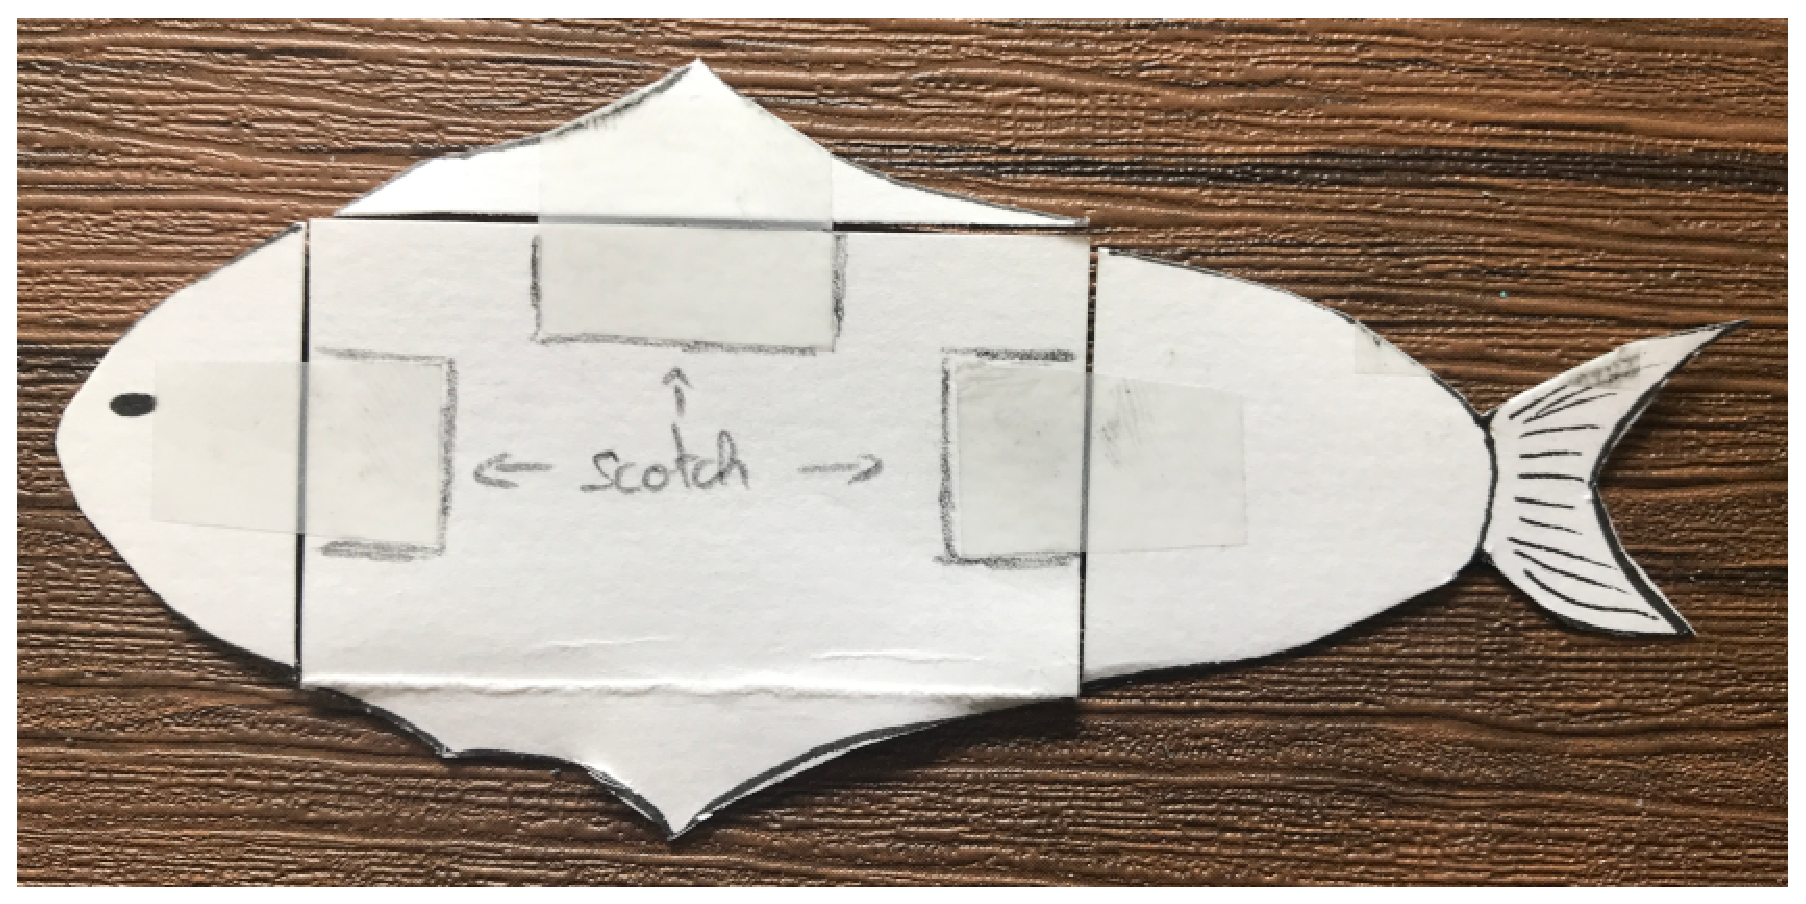
\includegraphics[width=8cm]{pavage4} 
      \end{minipage}
      \ \\ [5mm]
      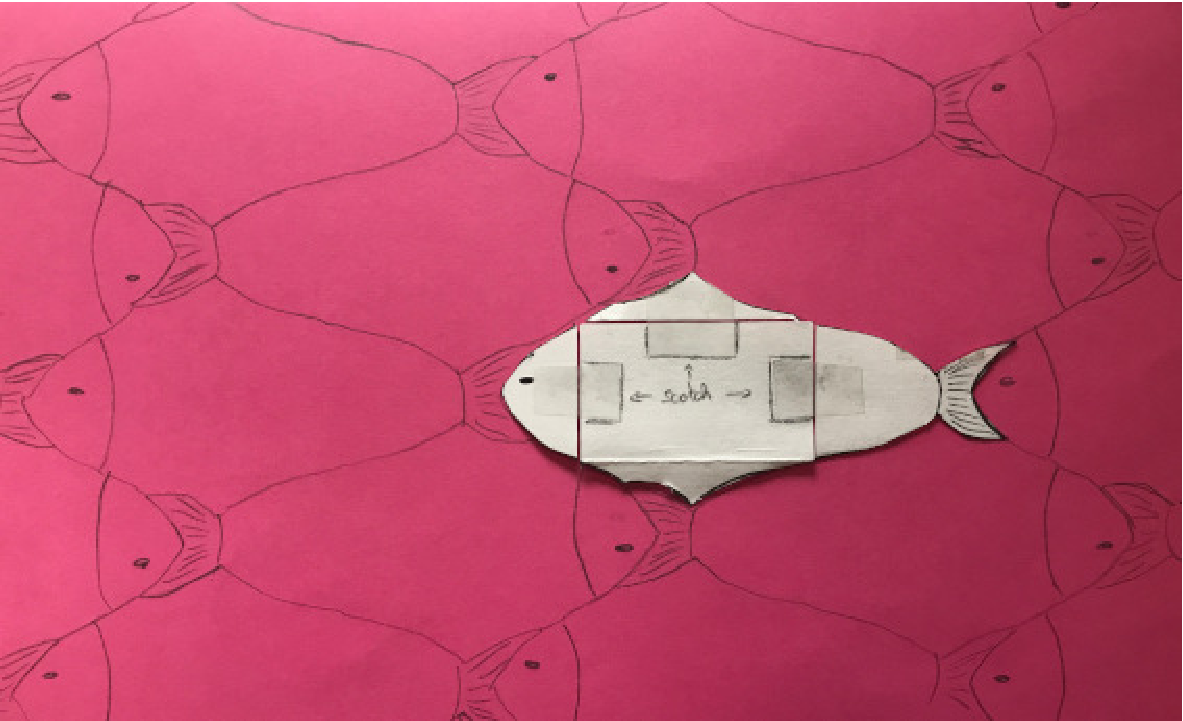
\includegraphics[width=14cm]{pavage5}
   \end{center}
 

%\themaM
\graphicspath{{../../S13_Calcul_d_aires/Images/}}

\chapter{Calcul d'aires}
\label{S13}


%%%%%%%%%%%%%%%%%%%%%%%%%%%%%%%%%%%%%
%%%%%%%%%%%%%%%%%%%%%%%%%%%%%%%%%%%%%
\begin{prerequis}
   \begin{itemize}
      \item[\com] Mener des calculs impliquant des grandeurs mesurables, notamment des grandeurs composées, exprimer les résultats dans les unités adaptées.
      \item[\com] Vérifier la cohérence des résultats du point de vue des unités.
      \item[\com] Effectuer des conversions d’unités.
   \end{itemize}
\end{prerequis}

\vfill

\begin{debat}[La quadrature du cercle]
   Dans le langage courant, l'aire désigne souvent une surface plane limitée, destinée à un usage précis : une aire de jeu, une aire d'atterrissage, une aire de lancement\dots{} \\
   En mathématiques, l'aire est la mesure d'une surface et a procuré de nombreuses recherches depuis très longtemps. Par exemple, {\bf la quadrature du cercle} consiste à trouver, par construction à la règle et au compas, un carré d'aire égale à un disque. Ce problème a été posé pendant l'Antiquité dans la civilisation grecque et a été réfuté seulement en 1882 par le mathématicien allemand {\it Ferdinand von Lindemann}. 
   \begin{center}
      \begin{pspicture}(0,0)(8.5,4.2)
         \pscircle*[linecolor=B3](2,2){2}
         \psline(2,2)(4,2)
         \rput(3,2.3){$R$}
         \rput(2,1.3){aire : $\pi R^2$}
         \psframe*[linecolor=A3](5,0.23)(8.54,3.77)
         \rput(6.8,2){aire : $\pi R^2$\;?}
      \end{pspicture}
   \end{center}
   \bigskip
   \begin{cadre}[B2][F4]
      \begin{center}
         Vidéo : \href{https://www.youtube.com/watch?v=TcNfC8b4hUg}{\bf Raconte-moi une histoire : Archimède et le nombre $\pi$}, chaîne YouTube {\it m@ths et tiques}, Yvan Monka.
      \end{center}
   \end{cadre}
\end{debat}

\vfill

\textcolor{PartieGeometrie}{\sffamily\bfseries Cahier de compétences} : chapitre 11, exercices 14 à 31.


%%%%%%%%%%%%%%%%%%%%%%%%%%%%%%%%%%%%
%%%%%%%%%%%%%%%%%%%%%%%%%%%%%%%%%%%%
\activites

\begin{activite}[Une aire multiforme]
   {\bf Objectifs :} tracer différentes figures d'aire donnée ; travailler les multiples et diviseurs.
   \begin{QCM}
      M. et Mme Vegetable veulent installer un potager de \umq{12} dans leur jardin. \\
         Ils souhaitent dessiner sur une feuille différentes formes correspondant à cette surface au 1/100\up{e}. \\
         Par combien de centimètre sera représentée une longueur de 1 mètre ? \pf \\
   
      \partie[des potagers rectangulaires]
      \ \\ [-10mm]
         \begin{enumerate}
            \item Pour délimiter leur potager, on propose à M. et Mme Vegetable des bordures de longueur \um{1} qu'ils ne veulent pas découper. Dessiner en rouge sur votre feuille toutes les possibilités de potagers rectangulaires qu'ils peuvent constituer avec de telles bordures.
            \item Ils décident de couper une bordure en deux. Dessiner en noir les nouveaux potagers rectangulaires qu'il est possible de construire.
            \item Dessiner en vert deux nouveaux potagers rectangulaire d'aire \umq{12} avec des mesures de votre choix.
            \item Rappeler la formule de calcul de l'aire d'un rectangle de côtés $L$ et $\ell$ puis compléter le tableau avec les valeurs trouvées aux questions 1), 2) et 3). \\
               \begin{minipage}{6cm}
                  \begin{pspicture}(-1,-0.75)(5,2.5)
                     \small
                     \psframe(0,0)(3.5,2)
                     \rput(1.75,-0.3){$L$}
                     \rput(3.8,1){$\ell$}
                     \rput(1.75,1){$\mathcal{A} =\hdashrule{16mm}{0.15pt}{4pt 2pt}$}
                  \end{pspicture}
               \end{minipage}
               \begin{minipage}{10cm}
                  {\hautab{1.5}
                  \begin{ctableau}{0.9\linewidth}{8}
                     \hline
                     \small $L$ & & & & & & & \\
                     \hline
                     \small $\ell$ & & & & & & & \\
                     \hline
                  \end{ctableau}}
               \end{minipage}
         \end{enumerate}

      \partie[des potagers triangulaires]
      \ \\ [-10mm]
          \begin{enumerate}
            \item M. et Mme Vegetable se disent qu'il serait original d'avoir un potager triangulaire. Ils souhaitent avoir une base de \um{6}. Dessiner en bleu trois potagers d'aire \umq{12} et de base \um{6}.
            \item Donner toutes les mesures possibles pour la base et la hauteur sachant que ces mesures sont des nombres entiers.
            \item Rappeler la formule de calcul de l'aire d'un triangle de base $B$ et de hauteur $h$ puis compléter le tableau avec les valeurs trouvées à la question 2). \\
               \begin{minipage}{7.5cm}
                  \begin{pspicture}(-1.5,-0.75)(5,2.5)
                     \pspolygon(0,0)(3.5,0)(2.5,2)
                     \psline[linestyle=dashed](2.5,0)(2.5,2)
                     \rput(1.75,-0.3){$B$}
                     \rput(2.8,1){$h$}
                     \psframe(2.5,0)(2.25,0.25)
                     \rput(-0.5,1.3){$\mathcal{A} =\hdashrule{16mm}{0.15pt}{4pt 2pt}$}
                  \end{pspicture}
               \end{minipage}
               \begin{minipage}{7cm}
                  {\hautab{1.5}
                  \begin{ctableau}{0.9\linewidth}{5}
                     \hline
                     \small $B$ & & & & \\
                     \hline
                     \small $h$ & & & & \\
                     \hline
                  \end{ctableau}}
               \end{minipage}
         \end{enumerate}
         
      \partie[un potager circulaire]
       \ \\ [-10mm]
        \begin{enumerate}
            \item Finalement, M. et Mme Vegetable s'orientent vers un potager circulaire. Donner une valeur au centième près de la valeur du rayon.
            \item Rappeler la formule de calcul de l'aire d'un disque de rayon $R$. \\
                  \begin{pspicture}(-9.5,-0.25)(3,1.5)
                     \pscircle(2,1){1}
                     \psline[linestyle=dashed](2,1)(3,1)
                     \rput(2.5,1.3){$R$}
                     \rput(5,1){$\mathcal{A} =\hdashrule{16mm}{0.15pt}{4pt 2pt}$}
                     \psdot(2,1)
                  \end{pspicture}
            \end{enumerate}
   \end{QCM}
\end{activite}


%%%%%%%%%%%%%%%%%%%%%%%%%%%%%%%%%%%%
%%%%%%%%%%%%%%%%%%%%%%%%%%%%%%%%%%%%
\cours 

\section{Aires usuelles} %%%

\medskip

\begin{Ltableau}{\linewidth}{4}{C{4}|p{2.6cm}|C{3.5}|p{5cm}}
   \hline 
   Figure plane & Mesures & Exemple & Calcul \\
   \hline
   \begin{pspicture}(0,0)(4,4) % rectangle
      \pstGeonode[PointName=none,linecolor=B2,PointSymbol=none](0.5,1){A}(3.5,1){B}(3.5,3){C}(0.5,3){D}
      \pstSegmentMark[linecolor=B2]{A}{B}
      \pstSegmentMark[SegmentSymbol=MarkCros,linecolor=A1]{B}{C}
      \pstSegmentMark[linecolor=B2]{C}{D}
      \pstSegmentMark[SegmentSymbol=MarkCros,linecolor=A1]{D}{A}
      \rput(2,2){\small rectangle}
      \rput(2,0.6){\textcolor{B2}{$L$}}
      \rput(3.8,2){\textcolor{A1}{$\ell$}}
   \end{pspicture}
   &
   \begin{minipage}[b]{3cm}
      $\mathcal{A} =L\times \ell$ \\ [10mm]
   \end{minipage}
   &
   \begin{pspicture}(0,-0.2)(4,4.1)
      \psframe[fillstyle=solid,fillcolor=lightgray!50](1,0.5)(3,3.5)
      \psline[linestyle=dashed]{<->}(1,0.2)(3,0.2)
      \rput(2,-0.1){\udm{0,2}}
      \psline[linestyle=dashed]{<->}(0.7,0.5)(0.7,3.5)
      \rput{90}(0.4,2){\udm{0,3}}
   \end{pspicture}
   &
   \begin{minipage}[b]{5cm}
      $\mathcal{A}=\udm{0,2}\times\udm{0,3} =\udmq{0,06}$ \\ [10mm]
   \end{minipage} \\
      \multicolumn{4}{|c|}{Pour le cas particulier du carré, on a $\mathcal{A} =c^2$ \, où $c$ est la mesure du côté du carré.} \\
   \hline
      \begin{pspicture}(0,-0.2)(4,4.2) % triangles
      \pstGeonode[PointName=none,PointSymbol=none](0.5,0.5){A}(3.5,0.5){B}(1,3.5){C}(1,0.5){H}
      \pstLineAB[linecolor=B2]{A}{B}
      \pstLineAB{A}{C}
      \pstLineAB{C}{B}
      \pstLineAB[linecolor=J1]{C}{H}
      \pstRightAngle[linecolor=J1]{B}{H}{C}
      \rput(1.9,1.2){\small triangle}
      \rput(2,0.2){\textcolor{B2}{$b$}}
      \rput(1.2,2){\textcolor{J1}{$h$}}
   \end{pspicture}
   &
   \begin{minipage}[b]{3cm}
      $\mathcal{A} =\dfrac{b\times h}{2}$ \\ [10mm]
   \end{minipage}
   &
   \begin{pspicture}(0,-0.2)(4,4.2)
      \pspolygon[fillstyle=solid,fillcolor=lightgray!50](0.5,3)(3.2,3)(2.5,0.4)
      \psline[linestyle=dashed]{<->}(0.5,3.3)(3.2,3.3)
      \psline(2.2,3)(2.2,2.7)(2.5,2.7)
      \rput(2,3.6){$27$ mm}
      \psline[linestyle=dashed]{<->}(2.5,0.4)(2.5,3)
      \rput{90}(2.15,2){$26$ mm}
   \end{pspicture}
   &
   \begin{minipage}[b]{5cm}
      $\mathcal{A} =\dfrac{\umm{27}\times\umm{26}}{2} =\ummq{351}$ \\ [10mm]
   \end{minipage} \\ 
      \multicolumn{4}{|c|}{Dans le cas du triangle rectangle, on choisit comme base et comme hauteur les deux côtés de l'angle droit.} \\
   \hline
   \begin{pspicture}(0,0.2)(4,3.8)
      \pscircle(2,2){1.3}
      \psdots(2,2)
      \psline[linecolor=B2,arrowsize=0.2]{<->}(2,2)(3.3,2)
      \rput(2.75,2.2){\textcolor{B2}{$r$}}
      \rput(2,1.6){disque}
   \end{pspicture}
   &
   \begin{minipage}[b]{3cm}
      $\mathcal{A} =\pi\times r\times r$ \\
      $\mathcal{A} =\pi r^2$ \\ [8mm]
   \end{minipage}
   &
   \begin{pspicture}(0.2,0.2)(4,3.8)
      \pscircle[fillstyle=solid,fillcolor=lightgray](2,2){1.3}
      \psline[linestyle=dashed,arrowsize=0.2]{<->}(2,2)(3.3,2)
      \rput(2.65,2.35){$1,2$ cm}
   \end{pspicture}
   &
   \begin{minipage}[b]{5cm}
      $\mathcal{A} =\pi\times(\ucm{1,2})^2\approx\ucmq{4,52}$ \\ [10mm]
   \end{minipage} \\
   \hline
\end{Ltableau}


\section{Calcul d'aires composées} %%%%%%%%

Pour calculer l'aire d'une figure complexe, il suffit de la \og découper \fg{} en figures usuelles et d'additionner ou de soustraire les aires qui la constituent.

\begin{exemple}
   \begin{pspicture}(-1,-0.5)(5,2.7)
         \pspolygon[fillstyle=solid,fillcolor=lightgray](0,0)(4,0)(3,2)(0,2)
         \psline{<->}(1,-0.3)(2,-0.3)
         \rput(1.5,-0.6){\ucm{1}}
         \psline[linestyle=dashed](3,2)(3,0)
         \pscircle[fillstyle=solid,fillcolor=white](1.5,1){0.5}
         \rput(-0.3,-0.3){$D$}
         \rput(-0.3,2.3){$A$}
         \rput(4.3,-0.1){$C$}
         \rput(3.2,2.3){$B$}
         \rput(3,-0.35){$M$}
         \psgrid[subgriddiv=2,gridcolor=darkgray,subgridcolor=darkgray,gridlabels=0](0,0)(4,2)
      \end{pspicture}
   \correction
      La figure grisée ci-contre est composée du rectangle $ABMD$ de longueur \ucm{3} et de largeur \ucm{2} ; du triangle $MBC$ de base \ucm{1} et de hauteur \ucm{2} et du disque de rayon \ucm{0,5}. \\
      Pour calculer son aire, on additionne l'aire du rectangle et du triangle et on soustrait l'aire du disque : \\ [1mm]
      $\mathcal{A} =\ucm{3}\times\ucm{2}+\dfrac{\ucm{1}\times\ucm{2}}{2}-\pi\times(\ucm{0,5})^2 \approx\ucmq{6,21}$
\end{exemple}


%%%%%%%%%%%%%%%%%%%%%%%%%%%%%%%
%%%%%%%%%%%%%%%%%%%%%%%%%%%%%%%
\exercicesbase

\begin{colonne*exercice}

\serie{Calcul d'aires} %%%

\medskip

\begin{exercice} %1
   Calculer l'aire de ces figures. \\
   {\psset{unit=0.45}
   \small
   \begin{pspicture}(-1,0)(13,6)
      \psframe(1,1)(7,5)
      \psframe(1,1)(1.4,1.4)
      \rput(4,1){/\!\!/}
      \rput(4,5){/\!\!/}
      \rput(1,3){$\times$}
      \rput(7,3){$\times$}
      \rput(4,0.2){\um{8}}
      \rput{90}(0.2,2.7){\um{4,5}}
      \rput(4,3){A}
      
      \psframe(10,1)(13,4)
      \psframe(10,1)(10.4,1.4)
      \rput(11.5,1){$\bullet$}
      \rput(11.5,4){$\bullet$}
      \rput(10,2.5){$\bullet$}
      \rput(13,2.5){$\bullet$}
      \rput(11.5,0.2){\umm{12,3}}
      \rput(11.5,2.5){B}
   \end{pspicture} \\

   \begin{pspicture}(-1,0)(13,5)
      \pspolygon(1,1)(7,1)(2,5)
      \psframe(2,1)(2.3,1.3)
      \psline(2,1)(2,5)
      \rput{-40}(5.2,3.5){\ucm{6,9}}
      \rput{78}(0.8,3.2){\ucm{4,6}}
      \rput(3.5,0){\ucm{6,6}}
      \rput{90}(2.5,2.7){\ucm{4,4}}
      \rput(3.8,2.2){C}
      
      \pspolygon(9,1)(14,1)(14,6)
      \psframe(14,1)(13.7,1.3)
      \rput(11.5,0){\ukm{8,5}}
      \rput(11.5,1){|\!\!|}
      \rput(14,3.5){=}
      \rput(12.5,2.5){D}
   \end{pspicture} \\
   
   \begin{pspicture}(-1,0.5)(13,5.5)
      \pscircle(3,3){2.5}
      \psline(3,3)(5.5,3)
      \rput(4.25,2.5){\udm{1,5}}
      \rput(3,3.75){E}
      \pscircle(12,3){2}
      \psline(10,3)(14,3)
      \rput(12,2.5){\um{5,6}}
      \rput(12,3.5){F}
   \end{pspicture}}
\end{exercice}

\begin{corrige}
   \textcolor{G1}{$\bullet$} Figure A : on a un rectangle d'aire $L\times\ell$. \\
      $\mathcal{A} =\um{8}\times\um{4,5} =\blue\umq{36}$. \\ [2mm]
   \textcolor{G1}{$\bullet$} Figure B : on a un carré d'aire $c\times c$. \\
      $\mathcal{A} =\umm{12,3}\times\umm{12,3} =\blue\umq{151,29}$. \\ [2mm]  
   \textcolor{G1}{$\bullet$} Figure C : on a un triangle d'aire $\dfrac{b\times h}{2}$. \\
      $\mathcal{A} =\dfrac{\ucm{6,6}\times\ucm{4,4}}{2}=\blue \ucmq{14,52}$.  \\ [2mm]  
   \textcolor{G1}{$\bullet$} Figure D : on a un triangle d'aire $\dfrac{b\times h}{2}$. \\
      $\mathcal{A} =\dfrac{\ukm{8,5}\times\ukm{8,5}}{2}=\blue \ukmq{36,125}$.  \\ [2mm]  
   \textcolor{G1}{$\bullet$}  Figure E : on a un disque d'aire $\pi r^2$. \\
      $\mathcal{A} =\pi\times\udm{1,5}^2 \approx\blue \udmq{7,07}$. \\ [2mm]
   \textcolor{G1}{$\bullet$}  Figure F : on a un disque d'aire $\pi r^2$. \\
      $\mathcal{A} =\pi\times\left(\dfrac{\um{5,6}}{2}\right)^2 \approx\blue \umq{24,63}$.        
\end{corrige}

\smallskip

\begin{exercice} %2
   \begin{enumerate}
      \item On peut regrouper les surfaces ci-dessous par deux ou par trois sauf une, laquelle ?
      \item Calculer alors l'aire de chaque surface.
   \end{enumerate}
   \begin{center}
      {\psset{unit=0.8}
      \small
      \begin{pspicture}(0,0)(8,13)
         \psgrid[subgriddiv=0,gridlabels=0,gridcolor=lightgray](0,0)(8,13)
         \rput[r](7.8,12.5){unités de longueur}
         \rput(7.5,11.7){$u$}
         \psline(7,12)(8,12)
         \psset{fillstyle=solid,fillcolor=lightgray}
         \pscustom{\psarc(2,11){1}{0}{180} \psarcn(1,10){1}{90}{0} \psarcn(3,10){1}{180}{90}}
         \rput(2,11.25){\small B}
         \pscustom{\psarc(5,11){1}{0}{180} \psline(4,11)(4,10) \psarc(4,11){1}{270}{0} \psarc(6,11){1}{180}{270} \psline(6,10)(6,11)}
         \rput(5,11.5){\small D}
         
         \pscustom{\psarc(2,8){1}{90}{180} \psarcn(1,7){1}{90}{0} \psarc(2,8){1}{270}{0} \psarcn(3,9){1}{270}{180}}
         \rput(2,8){\small P}
         \pscustom{\psarc(5,8){1}{180}{0} \psline(6,8)(7,8) \psarc(6,8){1}{0}{180} \psline(5,8)(4,8)}
         \rput(5.5,8){\small F}
         
         \pscustom{\psarc(5,5){1}{90}{180} \psarcn(4,4){1}{90}{0} \psline(5,4)(5,5)(6,5)(6,4) \psarcn(7,4){1}{180}{90} \psarc(6,5){1}{0}{90} \psline(6,6)(5,6)}
         \rput(6.5,5.5){\small H}
         \pscustom{\psarcn(1,4){1}{90}{0} \psarcn(3,4){1}{180}{90} \psarcn(3,6){1}{270}{180} \psarcn(1,6){1}{0}{270}}
         \rput(2,5){\small I}
         
         \pscircle(6,2){1}
         \rput(6,2){\small L}
         \pscustom{\psline(1,2)(1,3)(3,3) \psarcn(3,2){1}{90}{0} \psline(4,2)(2,2)(2,1) \psarc(1,1){1}{0}{90}}
         \rput(2.5,2.5){\small N}
      \end{pspicture}}
   \end{center}
\end{exercice}

\begin{corrige}
\ \\ [-5mm]
   \begin{enumerate}
      \item On peut regrouper B et P ; D, F et L ; N et H. \\
         {\blue La surface $I$ est seule}. \smallskip
      \item \textcolor{G1}{$\bullet$} Les figures B et P peuvent être recomposées en rectangle de mesures $2u$ et $u$, leur aire vaut {\blue $2u^2$}. \\ [2mm]
         \textcolor{G1}{$\bullet$} Les figures D, F et L peuvent être recomposées en disque de rayon $u$, leur aire veut {\blue $\pi u^2$}. \\ [2mm]
         \textcolor{G1}{$\bullet$} Les figures N et H peuvent être recomposées en rectangle de mesures $3u$ et $u$, leur aire veut {\blue $3u^2$}. \\ [2mm]
         \textcolor{G1}{$\bullet$} La figure I peut être vue comme un carré de côté $2u$ auquel on enlève quatre quarts de disques, soit un disque de rayon $u$. $\mathcal{A} =\blue 4u^2-\pi u^2$.
   \end{enumerate}
\end{corrige}


\serie{Problèmes} %%%

\begin{exercice} %3
   Résoudre les petits problèmes suivants :
   \begin{enumerate}
      \item Quelle est l'aire d'un carré de périmètre \ucm{32} ?
      \item Quel est le périmètre d'un rectangle de largeur \um{6} et d'aire \umq{48} ?
   \end{enumerate}
\end{exercice}

\begin{corrige}
   \ \\ [-5mm]
   \begin{enumerate}
      \item Le périmètre d'un carré vaut $4\times c$, donc $c =\ucm{32}\div4 =\ucm{8}$. \\
         L'aire du carré vaut $(\ucm{8})^2 =\blue\ucmq{64}$.
      \item L'aire d'un rectangle vaut $L\times\ell$. \\
         On a alors $L\times\um{6} =\umq{48}$ soit $L =\dfrac{\umq{48}}{\um{6}} =\um{8}$. \\ [1mm]
         Donc, le périmètre vaut $2\times(\um{8}+\um{6}) =\blue\um{28}$.
   \end{enumerate}
\end{corrige}


%\begin{exercice} %4
%   On a la figure suivante où $M$ est un point de $]DC[$ :
%   \begin{center}
%   \small
%   {\psset{unit=0.9}
%      \begin{pspicture}(0,-0.5)(5,2.5)
%         \pspolygon(0,0)(5,0)(2,2)(0,2)
%         \psline[linestyle=dashed](2,2)(1.5,0)
%         \psframe(0,0)(0.2,0.2)
%         \psframe(0,2)(0.2,1.8)
%         \rput(-0.3,-0.3){$D$}
%         \rput(-0.3,2.3){$A$}
%         \rput(5.3,0){$C$}
%         \rput(2,2.3){$B$}
%         \rput(1.5,-0.3){$M$}
%         \rput(1,2.3){\ucm{2}}
%         \rput{90}(-0.3,1){\ucm{3}}
%         \psline{<->}(0,-0.5)(5,-0.5)
%         \rput(2.5,-0.8){\ucm{6}}
%         \rput{-30}(4,1){\ucm{5}}
%      \end{pspicture}}
%   \end{center}
%   \begin{enumerate}
%      \item Déterminer la position du point $M$ pour que le périmètre du quadrilatère $ABMD$ soit égal au périmètre du triangle $BCM$ sachant que c'est un nombre entier.
%      \item On place le point $M$ tel que $ABMD$ soit un rectangle. \\
%      Calculer l'aire du rectangle $ABMD$ et celle du triangle $BMC$. Que remarque-t-on ?
%   \end{enumerate}
%\end{exercice}
%
%\begin{corrige}
%   \ \\ [-5mm]
%   \begin{enumerate}
%      \item On teste plusieurs valeurs pour la longueur $DM$ et on note $\mathcal{P}_1$ le périmètre du quadrilatère $ABMD$ et $\mathcal{P}_2$ celui du triangle $BCM$. \\
%      \begin{itemize}
%         \item Si $DM =\ucm{1}$, alors $MC =\ucm{5}$ et : \\
%            $\mathcal{P}_1 =\ucm{2}+\ucm{3}+\ucm{1}+MB =\ucm{6}+MB$ \\
%            $\mathcal{P}_2 =\ucm{5}+\ucm{5}+MB =\ucm{10}+MB$. \\
%            Les périmètres ne sont pas égaux.
%         \item Si $DM =\ucm{2}$, alors $MC =\ucm{4}$ et : \\
%            $\mathcal{P}_1 =\ucm{2}+\ucm{3}+\ucm{2}+MB =\ucm{7}+MB$ \\
%            $\mathcal{P}_2 =\ucm{5}+\ucm{4}+MB =\ucm{9}+MB$. \\
%            Les périmètres ne sont pas égaux.
%         \item Si $DM =\ucm{3}$, alors $MC =\ucm{3}$ et : \\
%            $\mathcal{P}_1 =\ucm{2}+\ucm{3}+\ucm{3}+MB =\ucm{8}+MB$ \\
%            $\mathcal{P}_2 =\ucm{5}+\ucm{3}+MB =\ucm{8}+MB$. \\
%            Les périmètres sont égaux.
%      \end{itemize}
%      Conclusion : le point $M$ doit être placé à {\blue \ucm{3} de $D$} pour que les périmètres soient égaux.
%      \item Si $ABMD$ est un rectangle, alors $DM =\ucm{2}$ \\
%      D'où $\mathcal{A}_{ABMD} =\ucm{3}\times\ucm{2} =\ucmq{6}$ ; \\ [1mm]
%      et $\mathcal{A}_{BMC} =\dfrac{\ucm{4}\times\ucm{3}}{2}=\ucmq{6}$. \\ [1mm]
%      Conclusion : {\blue les aires sont égales}.
%   \end{enumerate}
%\end{corrige}

\bigskip

\begin{exercice} %4
   Dans cette figure, on a : $AB =\ucm{9}$ ; $BC =\ucm{21}$ ; $CD =\ucm{11}$ ; $DE =\ucm{9}$ ; $EF =\ucm{11}$ ; $GH =\ucm{7}$.
   \begin{center}
   {\psset{unit=1.7}
      \small
      \begin{pspicture}(-0.25,0)(3.25,2.25)
         \psframe(0,0)(3,2)
         \pspolygon(2,0)(3,1)(1,2)(0,0.8)
         \rput(-0.2,-0.2){$G$}
         \rput(-0.2,2.2){$A$}
         \rput(3.2,-0.2){$E$}
         \rput(3.2,2.2){$C$}
         \rput(2,-0.2){$F$}
         \rput(3.2,1){$D$}
         \rput(1,2.2){$B$}
         \rput(-0.2,0.8){$H$}
      \end{pspicture}}
   \end{center}
   \begin{enumerate}
      \item Calculer le périmètre du rectangle $ACEG$.
      \item Calculer l'aire du quadrilatère $BDFH$.
   \end{enumerate}
\end{exercice}

\begin{corrige}
   \ \\ [-5mm]
   \begin{enumerate}
      \item $\mathcal{P}_{ACEG} =2\times(AC+CE)$. \\
         Or, $AC =AB+BC =\ucm{9}+\ucm{21} =\ucm{30}$ ;\\
         et $CE =CD+DE =\ucm{11}+\ucm{9} =\ucm{20}$. \\
         D'où $\mathcal{P}_{ACEG} =2\times(\ucm{30}+\ucm{20}) =\ucm{100}$. \\
         {\blue Le périmètre du rectangle $ACEG$ est de \ucm{100}}.
      \item Pour calculer l'aire du quadrilatère $BDFH$, on calcule l'aire du rectangle $ACEG$ auquel on soustrait l'aire de chacun des triangles rectangles $ABH$, $BCD$, $DEF$ et $FGH$. \\
      $\mathcal{A}_{ACEG} =AC\times CE =\ucm{30}\times\ucm{20} =\ucmq{600}$. \\ [1.5mm]
      $\mathcal{A}_{ABH} =\dfrac{HA\times AB}{2} =\dfrac{\ucm{13}\times\ucm{9}}{2} =\ucmq{58,5}$. \\ [1.5mm]
      $\mathcal{A}_{BCD} =\dfrac{BC\times CD}{2} =\dfrac{\ucm{21}\times\ucm{11}}{2} =\ucmq{115,5}$. \\ [1.5mm]
      $\mathcal{A}_{DEF} =\dfrac{DE\times EF}{2} =\dfrac{\ucm{9}\times\ucm{11}}{2} =\ucmq{49,5}$. \\ [1mm]
      $\mathcal{A}_{FGH} = \dfrac{FG\times GH}{2} =\dfrac{\ucm{19}\times\ucm{7}}{2} =\ucmq{66,5}$. \\ [1.5mm]
      $\mathcal{A}_{BDFH} =\ucmq{600}-\ucmq{58,5}-\ucmq{115,5}$ \\
      \hspace*{14mm} $-\ucmq{49,5}-\ucmq{66,5} =\ucmq{310}$. \\
      {\blue L'aire du quadrilatère $BDFH$ est de \ucmq{310}}.
   \end{enumerate}
\end{corrige}

\smallskip

\begin{exercice} %5
   Le drapeau suisse est constitué d'un fond rouge et d'une croix blanche en son centre. \\
   On considère un drapeau dont la largeur et la longueur sont de \ucm{20} et \ucm{35} et la largeur et la longueur de chaque bande blanche est de \ucm{4} par \ucm{15}.
   \begin{enumerate}
      \item Dessiner le drapeau suisse à l'échelle 1/5\up{e}.
      \item Calculer l'aire de la croix blanche dessinée.
      \item Calculer l'aire de la surface rouge dessiné.
   \end{enumerate}
\end{exercice}

\begin{corrige}
   \ \\ [-5mm]
   \begin{enumerate}
      \item À l'échelle 1/5\up{e}, il faut diviser toutes les mesures par 5. \\
      Le drapeau mesure \ucm{4} par \ucm{7} et les bandes blanches mesurent chacune \ucm{0,8} par \ucm{3}. \\ [2mm]
         \begin{pspicture}(0,0)(7,4)
            \psframe[fillstyle=solid,fillcolor=red,linecolor=red](0,0)(7,4)
            \psframe[fillstyle=solid,fillcolor=white,linecolor=white](2,1.6)(5,2.4)
            \psframe[fillstyle=solid,fillcolor=white,linecolor=white](3.1,0.5)(3.9,3.5)
         \end{pspicture}
      \item Les deux bandes sont des rectangles de longueur \ucm{0,8} et de largeur \ucm{3} donc, leur aire vaut $\ucm{0,8}\times\ucm{3} =\ucmq{2,4}$. \\
         Pour calculer l'aire de la croix blanche, il faut multiplier par deux l'aire d'une bande blanche et lui soustraire l'aire du carré central (qui sinon est compté deux fois) de mesure $(\ucm{0,8})^2 =\ucmq{0,64}$. \\
      Or, $2\times\ucmq{2,4}-\ucmq{0,64} =\ucmq{4,16}$. \\
      D'où : {\blue l'aire de la croix blanche vaut \ucmq{4,16}}.
   \end{enumerate}
   
\Coupe

   \begin{enumerate}
      \setcounter{enumi}{2}
      \item L'aire de la surface rouge du drapeau se calcule en soustrayant l'aire de la surface blanche au drapeau entier. \\
      L'aire du drapeau entier vaut $\ucm{4}\times\ucm{7} =\ucmq{28}$. \\
      Or, $\ucmq{28}-\ucmq{4,16} =\ucmq{23,84}$. \\
      D'où : {\blue l'aire de la surface rouge vaut \ucmq{23,84}}.
   \end{enumerate}
\end{corrige}

\bigskip


\begin{exercice} %6
   Calculer l'aire de cette figure. Donner la valeur exacte et une valeur approchée au centimètre près.
   \begin{center}
      {\psset{unit=1.25}
      \begin{pspicture}(0,0)(5,4)
         \psgrid[subgriddiv=0,gridlabels=0,gridcolor=lightgray](0,0)(5,4)
         \psset{linewidth=0.3mm}
         \psarc(3,0){3}{90}{180}
         \psarc(3,1){2}{0}{90}
         \psarc(4,1){1}{-90}{0}
         \psline(0,0)(4,0)
         \psline{<->}(0,3)(1,3)
         \rput(0.5,3.5){\small \ucm{4}}
         \psline(3,0)(3,3)
         \psline(3,1)(5,1)
         \psline(4,0)(4,1)
      \end{pspicture}}
   \end{center}
\end{exercice}

\begin{corrige}
   Cette figure est composée de trois quarts de disque de rayons respectifs \ucm{12} ; \ucm{8} et \ucm{4} et d'un carré de côté \ucm{4}. \\
   \textcolor{G1}{$\bullet$} Aire du quart de disque de rayon \ucm{12} : $\pi\times(\ucm{12})^2\div4 =36\pi\,\ucmq{}$ \\
   \textcolor{G1}{$\bullet$} Aire du quart de disque de rayon \ucm{8} : $\pi\times(\ucm{8})^2\div4 =16\pi\,\ucmq{}$ \\
   \textcolor{G1}{$\bullet$} Aire du quart de disque de rayon \ucm{4} : $\pi\times(\ucm{4})^2\div4 =4\pi\,\ucmq{}$ \\
   \textcolor{G1}{$\bullet$} Aire du carré de côté \ucm{4} : $(\ucm{4})^2 =\ucmq{16}$ \\
   Aire totale : $=36\pi\,\ucmq{}+16\pi\,\ucmq{}+4\pi\,\ucmq{}+\ucmq{16}$ \\
   $ =56\pi\,\ucmq{}+\ucmq{16} \approx\ucmq{192}$. \\
   {\blue L'aire de la figure vaut environ \ucmq{192}}. \vspace*{10cm}
  
\Coupe

\corec{La surface du disque selon Archimède}
\bigskip

\begin{enumerate}
   \item Ce disque a pour rayon \ucm{6}, donc son périmètre vaut $2\times\pi\times\ucm{6} =12\pi \approx{\blue \ucm{37,7}}$.
   \item {\blue La figure 2 \og ressemble \fg{} à un rectangle}.
   \item On peut mesurer à l'aide d'une règle, on trouve environ \ucm{18,7} pour la longueur et \ucm{6} pour la largeur. Or, l'aire d'un rectangle se calcule grâce à la formule \og longueur $\times$ largeur \fg{} ce qui donne {\blue \ucmq{112,2}}.
   \item On peut approximer la longueur de la courbe bleue par le demi-périmètre du disque, soit \\
      {\blue $L =2\times\pi\times R\div2 =\pi\times R$} et la largeur est égale au rayon soit {\blue $\ell =R$}.
   \item On en déduit la formule de l'aire : \\
      $\mathcal{A} =(\pi\times R)\times R$, soit {\blue $\mathcal{A} =\pi\times R^2$}.
   \item En découpant des portions de plus en plus petites, Archimède a pu considérer que la courbe bleue se rapprochait de plus en plus d'une droite de même longueur. \\
      Intuitivement, il touche du doigt le concept de limite qui émergera près de 20 siècles plus tard avec les mathématiciens (entre autres) Isaac Newton et Gottfried Wilhelm Leibniz, au 17\up{e} siècle.
\end{enumerate}

\end{corrige}

\end{colonne*exercice}



%%%%%%%%%%%%%%%%%%%%%%%%%%%%%%%%%%%%%
%%%%%%%%%%%%%%%%%%%%%%%%%%%%%%%%%%%%%
\Recreation

\vspace*{-5mm}

\enigme[La surface du disque selon Archimède]

   \partie[un peu d'histoire] \smallskip
      \begin{minipage}{11cm}
         Archimède de Syracuse $(-284 ; -212)$ est un des plus grands scientifiques de l'antiquité, né à Syracuse. \\
         Il est à l'origine de plusieurs découvertes, dont la poussée d'Archimède et de systèmes de leviers. En mathématiques, il serait le premier à avoir donné une méthode permettant de trouver une valeur approchée de $\pi$ par encadrement par des polygones et il a proposé des méthodes de calcul d'aires de certaines surfaces comme par exemple celle du disque.
      \end{minipage}
      \qquad
      \begin{minipage}{3cm}
         
\includegraphics[width=3cm]{Archimede}
      \end{minipage}
      
   \partie[la méthode d'Archimède] \smallskip
      \begin{minipage}{5cm}
         \begin{pspicture}(-2.5,-2.25)(2.5,2.25)
            \pscircle(0,0){2}
            \psline[linewidth=1mm](-2,0)(2,0)
            \psarc[linewidth=1mm,linecolor=red](0,0){2}{0}{180}
            \psarc[linewidth=1mm,linecolor=blue](0,0){2}{180}{0}
            \multido{\r=0+22.5}{16}{\psline(0,0)(2;\r)}
         \end{pspicture}
      \end{minipage}
      \qquad
      \begin{minipage}{10cm}
         \begin{itemize}
            \item Tracer sur une feuille au format A4 un disque de rayon \ucm{6}.
            \item Tracer un diamètre de ce cercle puis repasser en rouge l'un des demi-cercles et en bleu l'autre demi-cercle.
            \item Découper ce cercle en deux parts égales, puis quatre, puis huit, puis seize. Proposer une méthode pour cela (il est possible d'utiliser tout le matériel de géométrie). 
         \end{itemize}
         \begin{enumerate}
            \item Calculer la valeur du périmètre de ce disque : \pf
         \end{enumerate}
      \end{minipage} \\
      \begin{itemize}
         \item Assembler les portions de disque comme sur la {\it figure 1} ci-dessous.
         \item Découper l'un des deux portions de disque des extrémités en deux parts égales.
         \item Coller sur le cahier toutes les portions de disque selon la {\it figure 2}.
         \begin{center}
            \begin{pspicture}(-0.5,-0.5)(14.5,2.5)
               \def\portion{
                  \psline(2;101.25)(0,0)(2;78.75)(0.79,0)
                  \psarc[linewidth=1mm,linecolor=red](0,0){2}{78.35}{101.65}
                  \psarc[linewidth=1mm,linecolor=blue](2;78.75){2}{-101.65}{-78.35}}
               \multido{\n=0+0.79}{8}{\rput(\n,0){\portion}}
               \rput(3,-0.5){\it figure 1}
               \rput(7,1){$\Rightarrow$}
               \multido{\n=8+0.79}{9}{\rput(\n,0){\portion}}
               \psframe*[fillstyle=solid,fillcolor=white,linecolor=white](8,-0.1)(7.5,2.1)
               \psline(8,-0.05)(8,2.05)
               \psframe*[fillstyle=solid,fillcolor=white,linecolor=white](14.32,-0.1)(15.15,2.1)
               \psline(14.32,-0.05)(14.32,2.05)
               \rput(11.5,-0.5){\it figure 2}
            \end{pspicture}
         \end{center}
      \end{itemize}
      \begin{enumerate}
      \setcounter{enumi}{1}
         \item À quoi \og ressemble \fg{} la figure 2 obtenue ? \pf \medskip
         \item En s'appuyant sur les mesures prises sur la figure collée, donner une approximation de son aire : \pf
      \end{enumerate}
         
   \partie[vers la formule de l'aire du disque] \smallskip   
      On considère ici un cercle de rayon $R$ découpé de la même manière que dans la partie B. \\ [2mm]
      \begin{minipage}{9cm} 
         \begin{enumerate}
         \setcounter{enumi}{3}
            \item Sur la figure ci-contre, exprimer la longueur $L$ et la largeur $\ell$ en fonction de $R$ en considérant que la longueur $L$ est presque équivalente à la longueur de la courbe en bleu.
            \item En déduire la formule proposée par Archimède pour l'aire d'un disque : \pf \medskip
            \item Comment cette approximation peut-elle se justifier ?
         \end{enumerate}
      \end{minipage}
      \qquad
      \begin{minipage}{7cm}
         {\psset{unit=0.9}
         \begin{pspicture}(7,-0.5)(14.5,2.5)
            \def\portion{
               \psline(2;101.25)(0,0)(2;78.75)(0.79,0)
               \psarc[linewidth=1mm,linecolor=red](0,0){2}{78.35}{101.65}
               \psarc[linewidth=1mm,linecolor=blue](2;78.75){2}{-101.65}{-78.35}}
            \multido{\n=8+0.79}{9}{\rput(\n,0){\portion}}
            \psframe*[fillstyle=solid,fillcolor=white,linecolor=white](8,-0.1)(7.5,2.1)
            \psline(8,-0.05)(8,2.05)
            \psframe*[fillstyle=solid,fillcolor=white,linecolor=white](14.32,-0.1)(15.15,2.1)
            \psline(14.32,-0.05)(14.32,2.05)
            \rput(11.5,-0.5){$L=\dots$}
            \rput{90}(7.5,0.75){$\ell =\dots$}
         \end{pspicture}}
      \end{minipage}

      

%\themaN
\graphicspath{{../../S14_Comparaison_et_egalite_de_fractions/Images/}}

\chapter{Comparaison et\\égalité de fractions}
\label{S14}


%%%%%%%%%%%%%%%%%%%%%%%%%%%%%%%%%%%%%%%
%%%%%%%%%%%%%%%%%%%%%%%%%%%%%%%%%%%%%%%
\begin{prerequis}
   \begin{itemize}
      \item[\com] Effectuer des calculs et des comparaisons de pour traiter des problèmes (fractions).
   \end{itemize}
\end{prerequis}

\vfill

\begin{debat}[Débat : les fractions, ces nombres rompus !] 
   Tout nombre peut s'écrire de différentes façons : ils ont des habillages différents mais ont la même valeur. La façon dont on les écrit permet de pouvoir les comparer. Par exemple, la {\bf fraction} $\dfrac68$ possède (entre autres) les représentations suivantes :
   \begin{center}
      {\psset{unit=0.8}
      \begin{pspicture}(-4,-4)(4,4)  
         \textcolor{B1}{\large
         \multido{\n=5+60,\i=55+60}{6}{\psline(3;\n)(0,0)(3;\i)}
         \multido{\n=30+60,\i=-60+60,\r=120+60}{6}{\psarc(2.719;\n){1.268}{\i}{\r}}
         \pscircle[fillstyle=solid,fillcolor=yellow](0,0){1.3}
         \rput(0,0){\bf $\dfrac68$}
         \rput(2.7;30){75\,\%}
         \rput(2.7;-30){0,75}
         \rput(2.7;150){$\dfrac34$}
         \rput(2.7;-150){$\dfrac{75}{100}$}
         \rput(2.7;90){\pswedge[fillstyle=solid,fillcolor=B3](0,0){0.8}{0}{-90}
                              \pscircle(0,0){0.8}
                              \multido{\n=0+45}{8}{\psline(0,0)(0.8;\n)}}
          \rput(2.7;-90){\psline(-1,0)(1,0)  
          \rput(-1,-0.4){\footnotesize 0}
          \rput(1,-0.4){\footnotesize 1}
          \psline[linecolor=B1,linewidth=1mm](-1,0)(0.5,0) \multido{\r=-1+0.25}{9}{\rput(\r,0){|}}}}
      \end{pspicture}}
   \end{center}
   \bigskip
   \begin{cadre}[B2][F4]
      \begin{center}
         Vidéo : \href{https://www.youtube.com/watch?v=eawBr43xWf8}{\bf Les fractions}, site Internet {\it Le blob}, épisode de la série {\it Petits contes mathématiques}.
      \end{center}
   \end{cadre}
\end{debat}

\vfill

\textcolor{PartieGeometrie}{\sffamily\bfseries Cahier de compétences} : chapitre 2, exercices 1 à 29 ; 43 à 45.


%%%%%%%%%%%%%%%%%%%%%%%%%%%%%%%%%%%%
%%%%%%%%%%%%%%%%%%%%%%%%%%%%%%%%%%%%%
\activites

\begin{activite}[Des briques et des fractions]
   {\bf Objectifs :} utiliser des fractions pour exprimer une proportion ; produire des fractions égales, ranger des fractions. \\
   \begin{QCM}
      \partie[les légo®] \medskip
         \begin{minipage}{10cm}
            On choisit la brique de Lego® classique $u$ ci-contre que l'on prend comme unité et les onze briques $a$ à $k$. On considère que le volume d'une brique est proportionnel au nombre de \og boutons \fg{} présents sur le dessus.
         \end{minipage}
         \hspace{1cm}
         \begin{minipage}{5cm}
            $u$ : \includegraphics[width=3.15cm]{lego_4_2a}
         \end{minipage} \\ [10mm]
            $a$ : \includegraphics[width=5.22cm]{lego_8_2a} \qquad 
            $b$ : \includegraphics[width=3.6cm]{lego_6_2a} \qquad
            $c$ : \includegraphics[width=1.35cm]{lego_2_2a} \qquad
            $d$ : \includegraphics[width=1.8cm]{lego_3_2a} \\ [5mm]
            $e$ : \includegraphics[width=6.3cm]{lego_10_2a} \qquad
            $f$ : \includegraphics[width=0.9cm]{lego_1_1a} \qquad
            $g$ : \includegraphics[width=1.35cm]{lego_2_1a} \qquad
            $h$ : \includegraphics[width=2.7cm]{lego_4_1a} \\ [5mm]
            $i$ : \includegraphics[width=5.4cm]{lego_8_1a} \qquad
            $j$ : \includegraphics[width=1.98cm]{lego_3_1a} \qquad
            $k$ : \includegraphics[width=4.05cm]{lego_6_1a} \\
            
      \partie[les fractions]
         \begin{enumerate}
            \item Compléter les égalités suivantes à l'aide de nombres entiers, décimaux ou fractionnaires : \\ [-3mm]
               \begin{multicols}{6}
                  $a = \pfh u$ \\ [7mm]
                  $b = \pfh u$ \\ [7mm]
                  $c = \pfh u$ \\ [7mm]
                  $d = \pfh u$ \\ [7mm]
                  $e = \pfh u$ \\ [7mm]
                  $f = \pfh u$ \\ [7mm]
                  $g = \pfh u$ \\ [7mm]
                  $h = \pfh u$ \\ [7mm]
                  $i = \pfh u$ \\ [7mm]
                  $j = \pfh u$ \\ [7mm]
                  $k = \pfh u$ \\ [7mm]
               \end{multicols} \medskip
            \item Compléter les égalités suivantes à l'aide de fractions dont le dénominateur est 8 : \\ [-3mm]
               \begin{multicols}{6}
                  $a = \dfrac{\qquad}{8} u$ \\ [7mm]
                  $b = \dfrac{\qquad}{8} u$ \\ [7mm]
                  $c = \dfrac{\qquad}{8} u$ \\ [7mm]
                  $d = \dfrac{\qquad}{8} u$ \\ [7mm]
                  $e = \dfrac{\qquad}{8} u$ \\ [7mm]
                  $f = \dfrac{\qquad}{8} u$ \\ [7mm]
                  $g = \dfrac{\qquad}{8} u$ \\ [7mm]
                  $h = \dfrac{\qquad}{8} u$ \\ [7mm]
                  $i = \dfrac{\qquad}{8} u$ \\ [7mm]
                  $j = \dfrac{\qquad}{8} u$ \\ [7mm]
                  $k = \dfrac{\qquad}{8} u$ \\ [7mm]
               \end{multicols} \smallskip
            \item Classer les Lego® dans l'ordre croissant de leur volume : \\ [2mm]
               \pf
      \end{enumerate}
   \end{QCM}
\end{activite}


%%%%%%%%%%%%%%%%%%%%%%%%%%%%%%%%%%%%%%%%%
%%%%%%%%%%%%%%%%%%%%%%%%%%%%%%%%%%%%%%%%%
\cours 

\section{Rappels sur les fractions} %%%

\begin{definition}
   Soit $a$ et $b$ deux nombres ($b\neq0$). Le {\bf quotient} $\dfrac{a}{b}$ est le nombre qui, multiplié par $b$, donne $a$. \\
   Ce quotient, écrit sous forme d'une fraction, est le résultat d'une division : $\dfrac{a}{b} =a\div b$.
\end{definition}

\begin{exemple}
   La fraction $\dfrac73$ peut-être interprétée comme :
   \correction
   \ \\ [-10mm]
   \begin{itemize}
      \item $7\div3$, dont une valeur approchée est 2,33 ;
      \item sept tiers, c'est-à-dire sept fois un tiers ;
      \item le nombre qui, multiplié par 3, donne
      7 : $\dfrac73\times3 =7$.
   \end{itemize}
\end{exemple}


\section{Égalité de fractions} %%%

\begin{propriete}
   On ne change pas la valeur d'une fraction en multipliant ou en divisant le numérateur et le dénominateur par un même nombre relatif non nul. \\ [1mm]
   \hspace*{3cm} $\dfrac{b}{c} =\dfrac{b\times a}{c\times a}= \dfrac{ba}{ca}. \text{\quad On a aussi \quad }a\times\dfrac{b}{c}= \dfrac{a\times b}{c} =\dfrac{ab}{c}$
\end{propriete}

%\begin{preuve}
%   {\hautab{1.9}
%   \begin{tabular}{p{3.7cm}p{10cm}}
%      $(a\times c)\times\dfrac{b}{c} =a\times \left(c\times\dfrac{b}{c}\right)$ & associativité de la multiplication\\
%      $\hspace*{16mm} =a\times b$
%      & $\dfrac{b}{c}$ est le nombre qui, multiplié par $c$ donne $b$ donc $c\times\dfrac{b}{c} =b$ \\
%      donc, $\dfrac{b}{c} =\dfrac{a\times b}{a\times c}$ & puisque $\dfrac{a\times b}{a\times c}$ est le nombre qui, multiplié par $a\times c$ donne $a\times b$ \\
%   \end{tabular}}
%\end{preuve}

\begin{exemple*1}   
   $\dfrac12 =\dfrac{1\times2}{2\times2} =\dfrac24 =\dfrac{2\times2}{4\times2} = \dfrac48\dots \qquad ; \qquad 7\times\dfrac{3}{5} =\dfrac{7\times3}{5} =\dfrac{21}{5}$.
\end{exemple*1}

\begin{remarque}
   la propriété permet de {\bf simplifier} des fractions, ce qui  signifie écrire une fraction qui lui est égale, mais avec un numérateur et un dénominateur plus petits.
\end{remarque}

\begin{exemple*1}
   Pour simplifier $\dfrac{150}{180}$, on peut tout d'abord diviser le numérateur et le dénominateur \\ [1mm]
      par 10 : $\dfrac{150}{180} =\dfrac{150\div10}{180\div10} =\dfrac{15}{18}$, puis les diviser encore par 3 : $\dfrac{15}{18} =\dfrac{15\div3}{18\div3} =\dfrac56$.
\end{exemple*1}


\section{Comparaison de fractions} %%%

\begin{propriete}
   \begin{itemize}
      \item Pour comparer deux fractions ayant le même dénominateur, on compare uniquement le numérateur : la fraction la plus grande est celle dont le numérateur est le plus grand.
      \item Pour comparer deux fractions de dénominateurs différents, on modifie l'écriture des fractions pour qu'elles aient le même dénominateur. \\ [-8mm]
   \end{itemize}
\end{propriete}

\begin{exemple}
   Comparer les fractions suivantes : \smallskip
   \begin{itemize}
      \item $\dfrac35$ et $\dfrac45$. \medskip
      \item $\dfrac23$ et $\dfrac{7}{12}$.
   \end{itemize}
   \correction
   On a :
   \begin{itemize}
      \item $3<4$ donc $\dfrac35<\dfrac45$. \smallskip
      \item On remarque que $\dfrac23=\dfrac{2\times4}{3\times4}=\dfrac{8}{12}$. \\ [1mm]
      Comme $\dfrac{8}{12}>\dfrac{7}{12}$, alors $\dfrac23>\dfrac{7}{12}$.
   \end{itemize}
\end{exemple}


%%%%%%%%%%%%%%%%%%%%%%%%%%%%%%%%%%%%%%%%%%
%%%%%%%%%%%%%%%%%%%%%%%%%%%%%%%%%%%%%%%%%%
\exercicesbase

\begin{colonne*exercice}

\serie{Fractions}

\begin{exercice} %1
   Ecrire la fraction qui représente la partie colorée de chaque figure puis la simplifier si possible. \\
   \begin{center}
      {\psset{unit=0.6}
      \begin{pspicture}(-1,-1.5)(2.2,1)
         \psframe[fillstyle=solid,fillcolor=A2](0,0)(-1,-1)
         \psframe(-1,-1)(1,1)
         \psline(-1,0)(1,0)
         \psline(0,-1)(0,1)
         \rput(-1.4,0){$a$}
      \end{pspicture}
      \begin{pspicture}(-1,-1.5)(2.2,1)
         \pspolygon[fillstyle=solid,fillcolor=A2](0,0)(0,-1)(1,-1)(1,1)(1,1)(-1,1)(-1,0)
         \psframe(-1,-1)(1,1)
         \psline(-1,0)(1,0)
         \psline(0,-1)(0,1)
         \rput(-1.4,0){$b$}
      \end{pspicture}
      \begin{pspicture}(-1,-1.5)(2.2,1)
         \psframe[fillstyle=solid,fillcolor=A2](-1,-1)(1,0)
         \psframe(-1,-1)(1,1)
         \psline(-1,0)(1,0)
         \psline(0,-1)(0,1)
         \rput(-1.4,0){$c$}
      \end{pspicture}
      \begin{pspicture}(-1,-1.5)(1,1)
         \psframe[fillstyle=solid,fillcolor=A2](-1,-1)(1,1)
         \psline(-1,0)(1,0)
         \psline(0,-1)(0,1)
         \rput(-1.4,0){$d$}
      \end{pspicture} \\ \medskip
      
      \begin{pspicture}(-1,-1.5)(2.2,1)
         \pswedge[fillstyle=solid,fillcolor=B2](0,0){1}{30}{-30}
         \pscircle(0,0){1}
         \multido{\n=0+30}{12}{\psline(0,0)(1;\n)}
         \rput(-1.4,0){$e$}
      \end{pspicture}
      \begin{pspicture}(-1,-1.5)(2.2,1)
         \pswedge[fillstyle=solid,fillcolor=B2](0,0){1}{90}{180}
         \pscircle(0,0){1}
         \multido{\n=0+30}{12}{\psline(0,0)(1;\n)}
         \rput(-1.4,0){$f$}
      \end{pspicture}
      \begin{pspicture}(-1,-1.5)(2.2,1)
         \pswedge[fillstyle=solid,fillcolor=B2](0,0){1}{-120}{-60}
         \pscircle(0,0){1}
         \multido{\n=0+30}{12}{\psline(0,0)(1;\n)}
         \rput(-1.4,0){$g$}
      \end{pspicture}
      \begin{pspicture}(-1,-1.5)(1,1)
         \pswedge[fillstyle=solid,fillcolor=B2](0,0){1}{60}{-120}
         \pscircle(0,0){1}
         \multido{\n=0+30}{12}{\psline(0,0)(1;\n)}
         \rput(-1.4,0){$h$}
      \end{pspicture} \\ \medskip
      
      \begin{pspicture}(-1,-1.2)(2.2,1.3)
         \pspolygon[fillstyle=solid,fillcolor=H1](1.2;210)(0,-0.6)(1.2;90)
         \pspolygon(1.2;-30)(1.2;90)(1.2;210)
         \psline(0.6;150)(1.2;-30)
         \psline(0.6;30)(1.2;210)
         \psline(0,-0.6)(0,1.2)
         \rput(-1.4,0.25){$i$}
      \end{pspicture}
      \begin{pspicture}(-1,-1.2)(2.2,1.3)
         \pspolygon[fillstyle=solid,fillcolor=H1](0,0)(1.2;-30)(0,-0.6)
         \pspolygon[fillstyle=solid,fillcolor=H1](0,0)(1.2;210)(0.6;150)
         \pspolygon[fillstyle=solid,fillcolor=H1](0,0)(1.2;90)(0.6;30)
         \pspolygon(1.2;-30)(1.2;90)(1.2;210)
         \psline(0.6;150)(1.2;-30)
         \psline(0.6;30)(1.2;210)
         \psline(0,-0.6)(0,1.2)
         \rput(-1.4,0.25){$j$}
      \end{pspicture}
      \begin{pspicture}(-1,-1.2)(2.2,1.3)
         \pspolygon[fillstyle=solid,fillcolor=H1](0,0)(0.6;30)(1.2;90)(0.6;150)
         \pspolygon(1.2;-30)(1.2;90)(1.2;210)
         \psline(0.6;150)(1.2;-30)
         \psline(0.6;30)(1.2;210)
         \psline(0,-0.6)(0,1.2)
         \rput(-1.4,0.25){$k$}
      \end{pspicture}
      \begin{pspicture}(-1,-1.2)(1,1.3)
         \pspolygon[fillstyle=solid,fillcolor=H1](0,0)(0.6;30)(1.2;90)(1.2;210)(1.2;-30)
         \pspolygon(1.2;-30)(1.2;90)(1.2;210)
         \psline(0.6;150)(1.2;-30)
         \psline(0.6;30)(1.2;210)
         \psline(0,-0.6)(0,1.2)
         \rput(-1.4,0.25){$l$}
      \end{pspicture} \\ \medskip
      
      \begin{pspicture}(-1,-1.5)(2.2,1)
         \psgrid[subgriddiv=2,subgridcolor=black,subgridwidth=0.8pt,gridlabels=0](-1,-1)(1,1)
         \psframe[fillstyle=solid,fillcolor=J1](-1,0)(0,1)
         \rput(-1.4,0){$m$}
      \end{pspicture}
      \begin{pspicture}(-1,-1.5)(2.2,1)
         \psgrid[subgriddiv=2,subgridcolor=black,subgridwidth=0.8pt,gridlabels=0](-1,-1)(1,1)
         \psframe[fillstyle=solid,fillcolor=J1](-1,0)(0,1)
         \psframe[fillstyle=solid,fillcolor=J1](0,0.5)(0.5,0)
         \psframe[fillstyle=solid,fillcolor=J1](-1,-0.5)(-0.5,0)
         \rput(-1.4,0){$n$}
      \end{pspicture}
      \begin{pspicture}(-1,-1.5)(2.2,1)
         \psgrid[subgriddiv=2,subgridcolor=black,subgridwidth=0.8pt,gridlabels=0](-1,-1)(1,1)
         \psframe[fillstyle=solid,fillcolor=J1](-1,-1)(1,0)
         \psframe[fillstyle=solid,fillcolor=J1](-1,0)(0,1)
         \psframe[fillstyle=solid,fillcolor=J1](0,0)(0.5,0.5)
         \rput(-1.4,0){$p$}
      \end{pspicture}
      \begin{pspicture}(-1,-1.5)(1,1)
         \psgrid[subgriddiv=2,subgridcolor=black,subgridwidth=0.8pt,gridlabels=0](-1,-1)(1,1)
         \psframe[fillstyle=solid,fillcolor=J1](-1,-1)(0.5,0)
         \psframe[fillstyle=solid,fillcolor=J1](-1,0)(-0.5,1)
         \psframe[fillstyle=solid,fillcolor=J1](0.5,-0.5)(1,0)
         \rput(-1.4,0){$q$}
      \end{pspicture}}   
   \end{center}
\end{exercice}
      
\begin{corrige}
   \begin{colitemize}{3}
      \item $a =\blue \dfrac14$ \medskip
      \item $b =\blue \dfrac34$ \medskip
      \item $c =\blue \dfrac24 =\dfrac12$ \medskip
      \item $d =\blue \dfrac44 =1$ \medskip
      \item $e =\blue \dfrac{10}{12} =\dfrac56$ \medskip
      \item $f =\blue \dfrac{3}{12} =\dfrac14$
      \item $g =\blue \dfrac{2}{12} =\dfrac16$
      \item $h =\blue \dfrac{6}{12} =\dfrac12$
      \item $i =\blue \dfrac36 =\dfrac12$
      \item $j =\blue \dfrac36 =\dfrac12$
      \item $k =\blue \dfrac26 =\dfrac13$
      \item $l =\blue \dfrac56$
      \item $m =\blue \dfrac{4}{16} =\dfrac14$
      \item $n =\blue \dfrac{6}{16} =\dfrac38$
      \item $p =\blue \dfrac{13}{16}$
      \item $q =\blue \dfrac{9}{16}$
   \end{colitemize}
\end{corrige}
    
      
\begin{exercice} %2
   Dans chaque figure ci-dessous, colorier selon la fraction donnée.
   \begin{center}
   {\small
      \psset{unit=0.75}
      \begin{pspicture}(-1,-1.3)(2.5,1)
         \psframe(-1,-1)(1,1)
         \rput(1.25,0){$\dfrac13$}
      \end{pspicture}
      \begin{pspicture}(-1,-1.3)(2.5,1)
         \psframe(-1,-1)(1,1)
         \rput(1.25,0){$\dfrac34$}
      \end{pspicture}
      \begin{pspicture}(-1,-1.3)(1.5,1)
         \psframe(-1,-1)(1,1)
         \rput(1.25,0){$\dfrac58$}
      \end{pspicture} \\ \medskip
      
      \begin{pspicture}(-1,-1.3)(2.5,1)
         \pscircle(0,0){1}
         \rput(1.25,0){$\dfrac13$}
      \end{pspicture}
      \begin{pspicture}(-1,-1.3)(2.5,1)
         \pscircle(0,0){1}
         \rput(1.25,0){$\dfrac34$}
      \end{pspicture}
      \begin{pspicture}(-1,-1.3)(1.5,1)
         \pscircle(0,0){1}
         \rput(1.25,0){$\dfrac58$}
      \end{pspicture} \\ \medskip
      
      \begin{pspicture}(-1,-1.3)(2.5,1)
         \pspolygon(1;30)(1;90)(1;150)(1;210)(1;270)(1;330)
         \rput(1.25,0){$\dfrac13$}
      \end{pspicture}
      \begin{pspicture}(-1,-1.3)(2.5,1)
         \pspolygon(1;30)(1;90)(1;150)(1;210)(1;270)(1;330)
         \rput(1.25,0){$\dfrac34$}
      \end{pspicture}
      \begin{pspicture}(-1,-1.3)(1.5,1)
         \pspolygon(1;30)(1;90)(1;150)(1;210)(1;270)(1;330)
         \rput(1.25,0){$\dfrac56$}
      \end{pspicture} \\ \medskip

      \begin{pspicture}(-1,-1.3)(2.5,1)
         \pspolygon(-1,-0.33)(-1,0.33)(-0.33,0.33)(-0.33,1)(0.33,1)(0.33,0.33)(1,0.33)(1,-0.33)(0.33,-0.33)(0.33,-1)(-0.33,-1)(-0.33,-0.33)
         \rput(1.25,0){$\dfrac14$}
      \end{pspicture}
      \begin{pspicture}(-1,-1.3)(2.5,1)
         \pspolygon(-1,-0.33)(-1,0.33)(-0.33,0.33)(-0.33,1)(0.33,1)(0.33,0.33)(1,0.33)(1,-0.33)(0.33,-0.33)(0.33,-1)(-0.33,-1)(-0.33,-0.33)
         \rput(1.25,0){$\dfrac38$}
      \end{pspicture}
      \begin{pspicture}(-1,-1.3)(1.5,1)
         \pspolygon(-1,-0.33)(-1,0.33)(-0.33,0.33)(-0.33,1)(0.33,1)(0.33,0.33)(1,0.33)(1,-0.33)(0.33,-0.33)(0.33,-1)(-0.33,-1)(-0.33,-0.33)
         \rput(1.25,0){$\dfrac25$}
      \end{pspicture}}
   \end{center}
\end{exercice}

\begin{corrige}
   \ \\ [-3mm]
   {\small
      \psset{unit=0.6}
      \begin{pspicture}(-1,-1.2)(3,1)
         \psframe(-1,-1)(1,1)
         \psline(-0.33,-1)(-0.33,1)
         \psline(0.33,-1)(0.33,1)
         \psframe[fillstyle=solid,fillcolor=A2](-1,-1)(-0.33,1)
         \rput(1.5,0){$\dfrac13$}
      \end{pspicture}
      \begin{pspicture}(-1,-1.2)(3,1)
         \pspolygon[fillstyle=solid,fillcolor=A2](0,0)(0,-1)(1,-1)(1,1)(1,1)(-1,1)(-1,0)
         \psframe(-1,-1)(1,1)
         \psline(-1,0)(1,0)
         \psline(0,-1)(0,1)
         \rput(1.5,0){$\dfrac34$}
      \end{pspicture}
      \begin{pspicture}(-1,-1.2)(1.5,1)
         \pspolygon[fillstyle=solid,fillcolor=A2](0,0)(1,-1)(1,-1)(1,1)(1,1)(-1,1)(-1,0)
         \psframe(-1,-1)(1,1)
         \psline(-1,0)(1,0)
         \psline(0,-1)(0,1)
         \psline(-1,-1)(1,1)
         \psline(-1,1)(1,-1)
         \rput(1.5,0){$\dfrac58$}
      \end{pspicture} \\ \medskip
      
      \begin{pspicture}(-1,-1.2)(3,1)
         \pswedge[fillstyle=solid,fillcolor=B2](0,0){1}{0}{120}
         \pscircle(0,0){1}
         \multido{\n=0+120}{3}{\psline(0,0)(1;\n)}
         \rput(1.5,0){$\dfrac13$}
      \end{pspicture}
      \begin{pspicture}(-1,-1.2)(3,1)
         \pswedge[fillstyle=solid,fillcolor=B2](0,0){1}{0}{-90}
         \pscircle(0,0){1}
         \multido{\n=0+90}{4}{\psline(0,0)(1;\n)}
         \rput(1.5,0){$\dfrac34$}
      \end{pspicture}
      \begin{pspicture}(-1,-1.2)(1.5,1)
         \pswedge[fillstyle=solid,fillcolor=B2](0,0){1}{0}{225}
         \pscircle(0,0){1}
         \multido{\n=0+45}{8}{\psline(0,0)(1;\n)}
         \rput(1.5,0){$\dfrac58$}
      \end{pspicture} \\ \medskip
      
      \begin{pspicture}(-1,-1.2)(3,1)
         \pspolygon[fillstyle=solid,fillcolor=H1](0,0)(1;30)(1;90)(1;150)
         \multido{\n=30+120}{3}{\psline(0,0)(1;\n)}
         \pspolygon(1;30)(1;90)(1;150)(1;210)(1;270)(1;330)
         \rput(1.5,0){$\dfrac13$}
      \end{pspicture}
      \begin{pspicture}(-1,-1.2)(3,1)
         \pspolygon[fillstyle=solid,fillcolor=H1](1;30)(1;90)(1;150)(1;210)(1;270)(1;330)
         \pspolygon[fillstyle=solid,fillcolor=white](0,0)(0.87,0)(1;30)(0,1)
         \psline(0,-1)(0,1)
         \psline(-0.87,0)(0.87,0)
         \rput(1.5,0){$\dfrac34$}
      \end{pspicture}
      \begin{pspicture}(-1,-1.2)(1.5,1)
         \pspolygon[fillstyle=solid,fillcolor=H1](1;30)(1;90)(1;150)(1;210)(1;270)(1;330)
         \pspolygon[fillstyle=solid,fillcolor=white](0,0)(1;30)(0,1)
         \multido{\n=30+60}{6}{\psline(0,0)(1;\n)}
         \rput(1.5,0){$\dfrac56$}
      \end{pspicture} \\ \medskip

      \begin{pspicture}(-1,-1.5)(3,1)
         \pspolygon[fillstyle=solid,fillcolor=J1](0,0)(0.33,0.33)(0.33,1)(-0.33,1)(-0.33,0.33)
         \pspolygon(-1,-0.33)(-1,0.33)(-0.33,0.33)(-0.33,1)(0.33,1)(0.33,0.33)(1,0.33)(1,-0.33)(0.33,-0.33)(0.33,-1)(-0.33,-1)(-0.33,-0.33)
         \psline(-0.33,-0.33)(0.33,0.33)
         \psline(0.33,-0.33)(-0.33,0.33)
         \rput(1.5,0){$\dfrac14$}
      \end{pspicture}
      \begin{pspicture}(-1,-1.5)(3,1)
         \pspolygon[fillstyle=solid,fillcolor=J1](0,0)(1,0)(1,0.33)(0.33,0.33)(0.33,1)(-0.33,1)(-0.33,0.33)
         \pspolygon(-1,-0.33)(-1,0.33)(-0.33,0.33)(-0.33,1)(0.33,1)(0.33,0.33)(1,0.33)(1,-0.33)(0.33,-0.33)(0.33,-1)(-0.33,-1)(-0.33,-0.33)
         \pspolygon(-1,-0.33)(-1,0.33)(-0.33,0.33)(-0.33,1)(0.33,1)(0.33,0.33)(1,0.33)(1,-0.33)(0.33,-0.33)(0.33,-1)(-0.33,-1)(-0.33,-0.33)
         \psline(-0.33,-0.33)(0.33,0.33)
         \psline(0.33,-0.33)(-0.33,0.33)
         \psline(-1,0)(1,0)
         \psline(0,-1)(0,1)
         \rput(1.5,0){$\dfrac38$}
      \end{pspicture}
      \begin{pspicture}(-1,-1.5)(1.5,1)
         \psframe[fillstyle=solid,fillcolor=J1](-0.33,-0.33)(1,0.33)
         \pspolygon(-1,-0.33)(-1,0.33)(-0.33,0.33)(-0.33,1)(0.33,1)(0.33,0.33)(1,0.33)(1,-0.33)(0.33,-0.33)(0.33,-1)(-0.33,-1)(-0.33,-0.33)
         \psframe(-0.33,-0.33)(0.33,0.33)
         \rput(1.5,0){$\dfrac25$}
      \end{pspicture}}
\end{corrige}

%%%%%%%%%%%%%
\serie{Egalités et comparaisons}

\begin{exercice} %3
   Compléter avec le signe $=$ ou $\neq$. \medskip
   \begin{colenumerate}{3}
      \item $\dfrac{3+5}{7+5} \pfh \dfrac{3}{7}$ \bigskip
      \item $\dfrac{3\times5}{7\times5} \pfh \dfrac{3}{7}$ \bigskip
      \item $\dfrac{3\times7}{7\times3} \pfh \dfrac{3}{7}$ \medskip
      \item $\dfrac{33}{77} \pfh \dfrac{3}{7}$
      \item $\dfrac{7}{3} \pfh \dfrac{3}{7}$
      \item $\dfrac{3}{7} \pfh 3,7$
      \item $\dfrac{3}{7} \pfh \dfrac{30}{70}$
      \item $\dfrac{3}{3} \pfh \dfrac{7}{7}$
      \item $3 \pfh\dfrac{21}{7}$
   \end{colenumerate}
\end{exercice}

\begin{corrige}
    \begin{colenumerate}{3}
      \item $\dfrac{3+5}{7+5} \, {\blue \neq} \, \dfrac{3}{7}$ \medskip
      \item $\dfrac{3\times5}{7\times5} \, {\blue =} \, \dfrac{3}{7}$ \medskip
      \item $\dfrac{3\times7}{7\times3} \, {\blue \neq} \, \dfrac{3}{7}$ \medskip
      \item $\dfrac{33}{77} \, {\blue =} \,  \dfrac{3}{7}$
      \item $\dfrac{7}{3} \, {\blue \neq} \, \dfrac{3}{7}$
      \item $\dfrac{3}{7} \, {\blue \neq} \, 3,7$
      \item $\dfrac{3}{7} \, {\blue =} \, \dfrac{30}{70}$
      \item $\dfrac{3}{3} \, {\blue =} \, \dfrac{7}{7}$
      \item $3 \, {\blue =} \, \dfrac{21}{7}$
   \end{colenumerate}
\end{corrige}

\medskip

%\begin{exercice} %3
%   Par quel nombre faut-il :
%   \begin{enumerate}
%      \item multiplier 5 pour obtenir 3 ?
%      \item multiplier 19 pour obtenir 97 ?
%      \item multiplier 12 pour obtenir 11 ?
%   \end{enumerate}
%   Ecrire à chaque fois l'égalité obtenue.
%\end{exercice}
%
%\begin{corrige}
%   \ \\ [-5mm]
%   \begin{enumerate}
%      \item On multiplie 5 par $\blue\dfrac35$ pour obtenir 3 : $5\times\dfrac35 =3$. \smallskip
%      \item On multiplie 19 par $\blue\dfrac{97}{19}$ pour obtenir 97 : \\
%          \qquad $19\times\dfrac{97}{19} =97$.
%      \item On multiplie 12 par $\blue\dfrac{11}{12}$ pour obtenir 11 : \\
%         \qquad $12\times\dfrac{11}{12} =11$.
%   \end{enumerate}
%\end{corrige}


\begin{exercice} %4
   Compléter les fractions suivantes : \medskip
   \begin{enumerate}
      \item $\dfrac{1}{2} =\dfrac{\qquad\;}{14} =\dfrac{8}{\qquad\;} =\dfrac{\qquad\;}{50} =\dfrac{16}{\qquad\;} =\dfrac{64}{\qquad\;}$ \\ [2mm]
      \item $\dfrac{4}{5} =\dfrac{\qquad\;}{15} =\dfrac{8}{\qquad\;} =\dfrac{\qquad\;}{50} =\dfrac{16}{\qquad\;} =\dfrac{64}{\qquad\;}$ \\ [2mm]
      \item $\dfrac{11}{7} =\dfrac{\qquad\;}{14} =\dfrac{88}{\qquad\;} =\dfrac{\qquad\;}{49} =\dfrac{121}{\qquad\;} =\dfrac{550}{\qquad\;}$ \\
   \end{enumerate}
\end{exercice}

\begin{corrige}
   \ \\ [-5mm]
   \begin{enumerate}
      \item $\dfrac{1}{2} =\dfrac{\blue 7}{14} =\dfrac{8}{\blue 16} =\dfrac{\blue 25}{50} =\dfrac{16}{\blue 32} =\dfrac{64}{\blue 128}$ \\ [2mm]
      \item $\dfrac{4}{5} =\dfrac{\blue 12}{15} =\dfrac{8}{\blue 10} =\dfrac{\blue 40}{50} =\dfrac{16}{\blue 20} =\dfrac{64}{\blue 80}$ \\ [2mm]
      \item $\dfrac{11}{7} =\dfrac{\blue 22}{14} =\dfrac{88}{\blue 56} =\dfrac{\blue 77}{49} =\dfrac{121}{\blue 77} =\dfrac{550}{\blue 350}$
   \end{enumerate}
\end{corrige}

\medskip

\begin{exercice} %5
   Surligner d'une même couleur les nombres égaux. \\ [2mm]
   {\hautab{2}
   \begin{tabular}{|*{7}{C{0.8}}|}
      \hline
      $\dfrac{5}{4}$ & $\dfrac{54}{45}$ & $\dfrac{28}{42}$ & $\dfrac{12}{15}$ & $\dfrac{1}{2}$ & $\dfrac{9}{81}$ & $\dfrac{4}{6}$ \\ [2mm]
      $\dfrac{50}{40}$ & $\dfrac{27}{54}$ & $\dfrac{4}{36}$ & $\dfrac{36}{72}$ & $\dfrac{1}{9}$ & $\dfrac{4}{5}$ & $\dfrac{6}{5}$ \\ [2mm]
      \hline
   \end{tabular}} \\ [1mm]
\end{exercice}

\begin{corrige}
   \ \\ [-8mm]
   {\hautab{2}
   \begin{tabular}[t]{|*{7}{C{0.6}}|}
      \hline
      $\textcolor{red}{\dfrac{5}{4}}$ & $\textcolor{blue}{\dfrac{54}{45}}$ & $\textcolor{orange}{\dfrac{28}{42}}$ & $\textcolor{green}{\dfrac{12}{15}}$ & $\textcolor{violet}{\dfrac{1}{2}}$ & $\textcolor{teal}{\dfrac{9}{81}}$ & $\textcolor{orange}{\dfrac{4}{6}}$ \\
       $\textcolor{red}{\dfrac{50}{40}}$ & $\textcolor{violet}{\dfrac{27}{54}}$ & $\textcolor{teal}{\dfrac{4}{36}}$ & $\textcolor{violet}{\dfrac{36}{72}}$ & $\textcolor{teal}{\dfrac{1}{9}}$ & $\textcolor{green}{\dfrac{4}{5}}$ & $\textcolor{blue}{\dfrac{6}{5}}$ \\ [1mm]
      \hline
   \end{tabular}}
\end{corrige}

\medskip

\begin{exercice} %6
   Simplifier au maximum ces fractions. \medskip
   \begin{colenumerate}{4}
      \item $\dfrac{6}{10}$ \bigskip
      \item $\dfrac{18}{16}$ \bigskip
      \item $\dfrac{16}{28}$
      \item $\dfrac{30}{48}$
      \item $\dfrac{88}{33}$
      \item $\dfrac{55}{30}$
      \item $\dfrac{15}{75}$
      \item $\dfrac{108}{117}$
   \end{colenumerate}
\end{exercice}

\begin{corrige}
   \begin{colenumerate}{2}
      \item $\dfrac{6}{10} =\dfrac{\cancel2\times3}{\cancel2\times5} =\blue\dfrac35$ \medskip
      \item $\dfrac{18}{16} =\dfrac{\cancel2\times9}{\cancel2\times8} =\blue\dfrac98$ \medskip
      \item $\dfrac{16}{28} =\dfrac{\cancel4\times4}{\cancel4\times7} =\blue\dfrac47$ \medskip
      \item $\dfrac{30}{48} =\dfrac{\cancel6\times5}{\cancel6\times8} =\blue\dfrac58$ \medskip
      \item $\dfrac{88}{33} =\dfrac{\cancel{11}\times8}{\cancel{11}\times3} =\blue\dfrac83$ \medskip
      \item $\dfrac{55}{30} =\dfrac{\cancel5\times11}{\cancel5\times6} =\blue\dfrac{11}6$ \medskip
      \item $\dfrac{15}{75} =\dfrac{\cancel{15}\times1}{\cancel{15}\times5} =\blue\dfrac15$ \medskip
      \item $\dfrac{108}{117} =\dfrac{\cancel9\times12}{\cancel9\times13} =\blue\dfrac{12}{13}$
   \end{colenumerate}
\end{corrige}

\medskip

\begin{exercice} %7
   Comparer les fractions suivantes : \medskip
   \begin{colenumerate}{3}
      \item $\dfrac{1}{9} \pfh \dfrac{1}{3}$ \bigskip
      \item $\dfrac{4}{9} \pfh \dfrac{12}{9}$ \bigskip
      \item $\dfrac{18}{17} \pfh 1$ \bigskip
      \item $\dfrac{7}{19} \pfh \dfrac{7}{20}$
      \item $\dfrac{2}{3} \pfh \dfrac{4}{6}$
      \item $\dfrac{18}{13} \pfh \dfrac{15}{13}$
      \item $\dfrac{81}{91} \pfh \dfrac{81}{90}$
      \item $\dfrac{17}{10} \pfh 0,7$
      \item $\dfrac{2}{3} \pfh \dfrac{1}{4}$
   \end{colenumerate}
\end{exercice}

\begin{corrige}
   \begin{colenumerate}{3}
      \item $\dfrac{1}{9} \, {\blue <} \, \dfrac{1}{3}$ \smallskip
      \item $\dfrac{4}{9} \, {\blue <} \,\dfrac{12}{9}$ \smallskip
      \item $\dfrac{18}{17} \, {\blue >} \,1$
      \item $\dfrac{7}{19} \, {\blue >} \,\dfrac{7}{20}$
      \item $\dfrac{2}{3} \, {\blue =} \,\dfrac{4}{6}$
      \item $\dfrac{18}{13} \, {\blue >} \,\dfrac{15}{13}$
      \item $\dfrac{81}{91} \, {\blue <} \,\dfrac{81}{90}$
      \item $\dfrac{17}{10} \, {\blue >} \,0,7$
      \item $\dfrac{2}{3} \, {\blue >} \,\dfrac{1}{4}$
   \end{colenumerate}
\end{corrige}

\medskip

\begin{exercice} %8
   Pour chaque item, réduire les fractions au même dénominateur, les ranger dans l'ordre croissant puis en déduire le classement des fractions initiales dans l'ordre croissant. \medskip
   \begin{enumerate}
      \item $A =\dfrac12 \; ; \; B =\dfrac23 \; ; \; C =\dfrac56 \; ; \; D = \dfrac5{12} \; ; \; E =\dfrac7{24}$. \bigskip
      \item $F =\dfrac12 \; ; \; G =\dfrac34 \; ; \; H =\dfrac78 \; ; \; I = \dfrac{11}{16} \; ; \; J =\dfrac{23}{32}$.
   \end{enumerate}
\end{exercice}

\begin{corrige}
   \ \\ [-5mm]
   \begin{enumerate}
      \item Fractions de dénominateur 24. \\ [1.5mm]
         $A =\dfrac{1\times12}{2\times12} =\dfrac{12}{24} \qquad B =\dfrac{2\times8}{3\times8} =\dfrac{16}{24}$ \\ [1.5mm]
         $C =\dfrac{5\times4}{6\times4} =\dfrac{20}{24} \qquad D = \dfrac{5\times2}{12\times2} =\dfrac{10}{24} \qquad E =\dfrac{7}{24}$ \\ [1.5mm]
         $\dfrac{7}{24}<\dfrac{10}{24}<\dfrac{12}{24}<\dfrac{16}{24}<\dfrac{20}{24}\Rightarrow$ {\blue $E<D<A<B<C$} \\ [3mm]
      \item Fractions de dénominateur 32. \\ [1.5mm]
         $F =\dfrac{1\times16}{2\times16} =\dfrac{16}{32} \qquad G =\dfrac{3\times8}{4\times8} =\dfrac{24}{32}$ \\ [1.5mm]
         $H =\dfrac{7\times4}{8\times4} =\dfrac{28}{32} \qquad I = \dfrac{11\times2}{16\times2} =\dfrac{22}{32} \qquad J =\dfrac{23}{32}$ \\ [1.5mm]
         $\dfrac{16}{32}<\dfrac{22}{32}<\dfrac{23}{32}<\dfrac{23}{32}<\dfrac{24}{32} \Rightarrow$ {\blue $F<I<J<G<H$} \\ [3mm]
   \end{enumerate}
   
\bigskip
\corec{ExploRATIO}
\bigskip

   \begin{ltableau}{\linewidth}{8}
      \hline
      \multicolumn{8}{|c|}{Niveau 1} \\
      \hline
      1a & 1b & 1c & 1d & 1e & 1f & 1g & 1h \\
      \hline
      & & & & & & & \\ [-4mm]
      $\dfrac27$ & $\dfrac38$ & $\dfrac14 $ & $\dfrac25$ & $\dfrac78$ & $\dfrac34$ & $\dfrac76$ & $\dfrac75$ \\
      & & & & & & & \\ [-4mm]
      \hline
   \end{ltableau}
   
   \begin{ltableau}{\linewidth}{8}
      \hline
      \multicolumn{8}{|c|}{Niveau 2} \\
      \hline
      2a & 2b & 2c & 2d & 2e & 2f & 2g & 2h \\
      \hline
      & & & & & & & \\ [-4mm]
      $\dfrac14$ & $\dfrac18$ & $\dfrac16$ & $\dfrac{1}{18}$ & $\dfrac{11}{24}$ & $\dfrac13$ & $\dfrac89$ & $\dfrac13$ \\
      & & & & & & & \\ [-4mm]
      \hline
   \end{ltableau}
   
   \begin{ltableau}{\linewidth}{7}
      \hline
      \multicolumn{7}{|c|}{Niveau 3} \\
      \hline
      2i & 2j & 2k & 2l & 2m & 2n & 2p \\
      \hline
      & & & & & & \\ [-4mm]
      $\dfrac{13}{6}$ & $\dfrac23$ & $\dfrac35$ & $\dfrac23$ & $1$ & $\dfrac12$ & $\dfrac38$ \\
      & & & & & & \\ [-4mm]
      \hline
   \end{ltableau}
\end{corrige}


\end{colonne*exercice}


%%%%%%%%%%%%%%%%%%%%%%%%%%%%%%%%%%%%%%%%%%
\Recreation

\enigme[ExploRATIO]
   \partie[présentation du matériel] 
      ExploRATIO est un matériel permettant des activités de manipulation et de réflexion dans le domaine des fractions. \\
      Il est composé de {\bf transparents} représentant un carré unité, puis un carré partagé en 2, en 3, en 4, en 5, en 6, en 7, en 8, en 9 et en 10 et de {\bf vignettes} dont une partie est colorée. \\
      L'objectif est de déterminer la fraction de l'unité correspondant à la partie colorée. \\ [3mm]
      {\it Exemple de vignette :
      \begin{center}
         \psset{unit=0.5}
         \begin{pspicture}(0,-1)(30,10)
            \psframe(0,0)(10,10)
            \psset{fillstyle=solid,fillcolor=A1}
            \psframe[linecolor=A1](1.43,0)(5.71,10)
            \rput(15,5){\parbox{4cm}{le transparent divisé en 7 parts égales permet de vérifier que la partie colorée correspond à trois septièmes d'unité, soit $\dfrac37$.}}
            \psframe[fillcolor=lightgray!50](20,0)(30,10)
            \psframe(21.43,0)(25.71,10)
            \multido{\n=21.43+1.43}{6}{\psline(\n,0)(\n,10)}
            \rput(29.6,9.5){7}
            \rput{90}(20.6,1.8){\footnotesize\gray ExploRATIO}
         \end{pspicture}
       \end{center}}

   \partie[À vous de jouer !]
      Pour chacun des niveaux 1, 2 et 3, donner la fraction de carré unité coloriée puis simplifier au maximum.
      \begin{center}
         \begin{ltableau}{\linewidth}{8}
            \hline
            \multicolumn{8}{|c|}{Niveau 1} \\
            \hline
            1a & 1b & 1c & 1d & 1e & 1f & 1g & 1h \\
            \hline
            & & & & & & & \\
            & & & & & & & \\
            & & & & & & & \\
            \hline
         \end{ltableau}
         \bigskip
         \begin{ltableau}{\linewidth}{8}
            \hline
            \multicolumn{8}{|c|}{Niveau 2} \\
            \hline
            2a & 2b & 2c & 2d & 2e & 2f & 2g & 2h \\
            \hline
            & & & & & & & \\
            & & & & & & & \\
            & & & & & & & \\
            \hline
         \end{ltableau}
         \bigskip
         \begin{ltableau}{\linewidth}{7}
            \hline
            \multicolumn{7}{|c|}{Niveau 3} \\
            \hline
            2i & 2j & 2k & 2l & 2m & 2n & 2p \\
            \hline
            & & & & & & \\
            & & & & & & \\
            & & & & & & \\
            \hline
         \end{ltableau}
      \end{center}
      
  
\vfill\hfill{\footnotesize \href{https://wp.gem-math.be/2021/02/04/exploratio-2/}{ExploRATIO : Un dispositif pédagogique créé par le 
Groupe d’Enseignement Mathématique (Belgique)}}


%\themaG
\graphicspath{{../../S15_Inegalite_triangulaire/Images/}}

\chapter{L'inégalité\\triangulaire}
\label{S15}


%%%%%%%%%%%%%%%%%%%%%%%%%%%%%%%%%%%%%%%%%%
\begin{prerequis}
   \begin{itemize}
      \item Inégalité triangulaire.
      \item[\com] Mettre en \oe uvre ou écrire un protocole de construction d’une figure géométrique.
   \end{itemize}
\end{prerequis}

\vfill

\begin{debat}[Débat : des instruments de navigation astronomique anciens] 
   De tous temps, les hommes ont cherché à se repérer. Avant l'avénement de l'électronique et des GPS, de multiples instruments ont pu exister, par exemple : 
   \begin{center}
   \textcolor{B1}{\small
      \begin{tabular}{*{5}{C{3}}}
         \includegraphics[height=3cm]{sphere} & \includegraphics[height=3cm]{astrolabe} & \includegraphics[height=3cm]{boussole}  & \includegraphics[height=3cm]{octant} & \includegraphics[height=3cm]{sextant} \\
        Sphère armillaire : & Astrolabe : & Boussole : & Octant : & Sextant : \\
        modélisation de la sphère céleste & représentation plane de la sphère armillaire & indique le nord magnétique & mesure la hauteur des corps célestes (\udeg{45}) & mesure la hauteur des corps célestes (\udeg{60}) \\
        & & & & \\
        Antiquité & Antiquité & {\small XIII}\up{e} & {\small XVIII}\up{e} & {\small XVIII}\up{e} \\
     \end{tabular}}
   \end{center}
   \bigskip
   \begin{cadre}[B2][F4]
      \begin{center}
         Vidéo : \href{https://www.youtube.com/watch?v=E0KvuFx0Mr8}{\bf Du kamal au GPS 1} et \href{https://www.youtube.com/watch?v=Jv21tvyZokk}{\bf Du kamal au GPS 2}, chaîne Youtube du {\it Musée national de la marine}. 
      \end{center}
   \end{cadre}
\end{debat}

\vfill

\textcolor{PartieGeometrie}{\sffamily\bfseries Cahier de compétences} : chapitre 8, exercices 1 à 17 ; 27 à 33.


%%%%%%%%%%%%%%%%%%%%%%%%%%%%%%%%%%%%%%%%
\activites

\begin{activite}[Avec des allumettes]
   {\bf Objectifs :} construire des triangles sous contraintes.
   \begin{QCM}
      Devant vous, vous avez dix allumettes. Pour chacune des questions suivantes, faire la construction si elle est possible avec des allumettes puis faire un dessin pour schématiser la situation.
      \begin{enumerate}
         \item
         \begin{enumerate}
            \item Aligner quatre allumettes en les plaçant les unes à côté des autres.
            \bigskip
            \begin{center}
               \includegraphics[width=3cm]{allumette}\includegraphics[width=3cm]{allumette}\includegraphics[width=3cm]{allumette}\includegraphics[width=3cm]{allumette}
            \end{center}
            \bigskip
            \item À partir de ce segment de longueur 4 allumettes, construire un triangle dont les deux autres côtés ont pour longueur trois allumettes. \\ [2cm]
            \item En utilisant les dix allumettes, construire un triangle différent du précédent dont un des côtés a pour longueur quatre allumettes. Quelles sont les longueurs de ses côtés ? \\ [2cm]
         \end{enumerate}
         \item En utilisant les dix allumettes, est-il possible de construire un triangle dont un des côtés a pour longueur six allumettes ? sept allumettes ? Expliquer. \\ [2cm]
         \item En utilisant les dix allumettes, peut-on construire un triangle dont un côté a pour longueur cinq allumettes ? Que constate-t-on dans ce cas ? \\ [2cm]
         \item On veut maintenant construire un triangle de périmètre 15 allumettes dont les côtés ont pour longueur un nombre entier d'allumettes. Donner toutes les solutions possibles. \\ [2cm]
      \end{enumerate}
   \end{QCM}
\end{activite}


%%%%%%%%%%%%%%%%%%%%%%%%%%%%%%%%%%%%%
%%%%%%%%%%%%%%%%%%%%%%%%%%%%%%%%%%%%%
\cours 

\section{L'inégalité triangulaire} %%%

\begin{propriete}
   Dans un triangle, la longueur d'un côté est toujours inférieure à la somme des longueurs des deux autres côtés. S'il y a égalité, alors les trois points sont alignés et le triangle est \og plat \fg.
\end{propriete}

\medskip

\begin{exemple}
   \begin{center}
   {\small
      \begin{pspicture}(0,-0.3)(3.5,2)
         \pstGeonode[CurveType=polygon,PointSymbol=none,PosAngle={180,90,0}](0,0){A}(2.5,2){C}(3.5,0){B}
         \pstLabelAB[offset=-3mm]{A}{B}{\ucm{3,5}}
         \pstLabelAB{A}{C}{\ucm{3,2}}
         \pstLabelAB{C}{B}{\ucm{2,2}}
      \end{pspicture}}
   \end{center}
   \correction
   Dans le triangle $ABC$, on a :
   \begin{itemize}
      \item $AC =\ucm{3,2}$ et $AB+BC =\ucm{5,7}$ donc $AC\leq AB+BC$ ;
      \item $CB =\ucm{2,2}$ et $CA+AB =\ucm{6,7}$ donc $CB\leq CA+AB$ ;
      \item $BA =\ucm{3,5}$ et $BC+CA =\ucm{5,4}$ donc $BA\leq BC+CA$.
   \end{itemize}
\end{exemple}

\smallskip

\begin{remarque}
   dans la pratique, on vérifie seulement que la longueur du plus grand côté est plus grande que la somme des longueurs des deux autres côtés.
\end{remarque}


\section{Construction de triangles} %%%

Pour construire un triangle, il faut au minimum trois données : \\
   - soit trois longueurs ; \\
   - soit deux longueurs et l'angle compris entre les segments correspondants aux longueurs données ; \\
   - soit une longueur et les deux angles adjacents au segment correspondant à la longueur donnée ; \\
   - si on a trois angles, on pourra construire un triangle mais il ne sera pas unique : tous les triangles seront semblables (des agrandissements ou des réductions du même triangle).

\bigskip

\begin{methode*1}[Construction d'un triangle connaissant trois longueurs]
   Pour construire un triangle $ABC$ dont on connaît les longueurs des trois côtés :
   \begin{itemize}
      \item on trace à la règle graduée l'un des côtés (en général le plus grand), par exemple $[AB]$ ;
      \item on trace un arc de cercle de centre $A$ et de rayon $AC$ ;
      \item on trace un arc de cercle de centre $B$ et de rayon $BC$ ;
      \item le point $C$ se situe à l'intersection des deux arcs de cercle.
   \end{itemize}
   \exercice
      Tracer le triangle $ABC$ tel que : $AB =\ucm{3,5}$ ; $BC =\ucm{2,2}$ et $CA =\ucm{3,2}$.
   \correction
         \ \\
         {\small
         \psset{unit=0.8}
         \begin{pspicture}(-0.5,-1.5)(4.8,2.8)
            \pstGeonode[PosAngle={225,-45}](0,0){A}(3.5,0){B}
            \pstLineAB{A}{B}
            \pstLabelAB[offset=-3mm]{A}{B}{\ucm{3,5}}
         \end{pspicture}
         \begin{pspicture}(0,-1.5)(4.8,2.8)
            \pstGeonode[PosAngle={225,-45}](0,0){A}(3.5,0){B}
            \pstLineAB{A}{B}
            \psset{linecolor=A1}
            \psarc(0,0){3.2}{30}{60}
            \rput{55}(0.8,1.3){\textcolor{A1}{\ucm{3,2}}}
            \compas{1.5}{1.2}{55}{0.9}{34.5}
         \end{pspicture}
         \begin{pspicture}(0,-1.5)(4.8,2.8)
            \pstGeonode[PosAngle={225,-45}](0,0){A}(3.5,0){B}
            \pstLineAB{A}{B}
            \psset{linecolor=A1}
            \psarc(0,0){3.2}{30}{60}
            \psset{linecolor=B1}
            \psarc[fillstyle=none](3.5,0){2.2}{90}{130}
            \rput{-45}(2.8,0.8){\textcolor{B1}{\ucm{2,2}}}
            \compas{3.3}{1.1}{130}{0.9}{23}
         \end{pspicture}
         \begin{pspicture}(0,-1.5)(2,2.8)
            \pstGeonode[CurveType=polygon,PointSymbol=none,PosAngle={225,90,-45}](0,0){A}(2.5,2){C}(3.5,0){B}
         \end{pspicture}}
\end{methode*1}


\begin{methode*1}[Construction d'un triangle connaissant deux longueurs et un angle]
   Pour construire un triangle $ABC$ dont on connait la longueur de deux côtés ainsi que l'angle entre ces cotés :
   \begin{itemize}
      \item on trace à la règle graduée l'un des côtés donnés, par exemple $[AB]$ ;
      \item on trace au rapporteur l'angle donné à partir du segment tracé ;
      \item on trace à la règle graduée le deuxième segment de longueur donnée le long du support de l'angle tracé juste avant ;
      \item le point $C$ se trouve à l'extrémité de ce segment.
   \end{itemize}
   \exercice
      Tracer le triangle $ABC$ tel que : $AB =\ucm{3,5}$ ; $\widehat{BAC} =39$\degre et $CA =\ucm{3,2}$.
   \correction
     \ \\
      {\small
      \psset{unit=0.8}
      \begin{pspicture}(-0.5,-1.5)(4.5,3)
         \pstGeonode[PosAngle={225,-45}](0,0){A}(3.5,0){B}
         \pstLineAB{A}{B}
         \pstLabelAB[offset=-3mm]{A}{B}{\ucm{3,5}}
      \end{pspicture}
      \begin{pspicture}(-3,-1.5)(4.1,3)
         \pstGeonode[PosAngle={225,-45}](0,0){A}(3.5,0){B}
         \pstLineAB{A}{B}  
         \psset{linecolor=A1}
         \rapporteur{0}{0}{0}{0.75}
         \psline(0,0)(4;38.66)
         \psarc(0,0){1}{0}{39}
         \rput(1.4,0.4){\textcolor{A1}{39\degre}}
      \end{pspicture}
      \begin{pspicture}(-1,-1.5)(3,3)
         \pstGeonode[CurveType=polygon,PointSymbol=none,PosAngle={225,90,-45}](0,0){A}(2.5,2){C}(3.5,0){B}
         \psline(0,0)(4;38.66) 
         \psline[linecolor=B1,linewidth=0.8mm](0,0)(2.5,2)
         \rput{40}(1.1,1.4){\textcolor{B1}{3,2 cm}}
      \end{pspicture}}
\end{methode*1}

\ \\ [5mm]

\begin{methode*1}[Construction d'un triangle connaissant une longueur et deux angles]
   Pour construire un triangle $ABC$ dont on connait la longueur d'un côté ainsi que ses deux angles adjacents :
   \begin{itemize}
      \item on trace à la règle graduée le côté donné, par exemple $[AB]$ ;
      \item on trace au rapporteur les deux angles donnés à partir du segment tracé ;
      \item les deux demi-droites tracées grâce au rapporteur se coupent au point $C$.
   \end{itemize}
   \exercice
      Tracer le triangle $ABC$ tel que : $AB =\ucm{3,5}, \widehat{BAC} =39$\degre et $\widehat{ABC} =63$\degre
   \correction
      \ \\
      {\small
      \psset{unit=0.8}
      \begin{pspicture}(-0.5,-1.5)(4.5,3.3)
         \pstGeonode[PosAngle={225,-45}](0,0){A}(3.5,0){B}
         \pstLineAB{A}{B}
         \rput(1.75,-0.25){3,5 cm}
      \end{pspicture}
      \begin{pspicture}(-3,-1.5)(4.1,3.3)
         \pstGeonode[PosAngle={225,-45}](0,0){A}(3.5,0){B}
         \pstLineAB{A}{B}  
         \psset{linecolor=A1}
         \rapporteur{0}{0}{0}{0.75}
         \psline(0,0)(4;38.66)
         \psarc(0,0){1}{0}{39}
         \rput(1.4,0.4){\textcolor{A1}{39\degre}}
      \end{pspicture}
      \begin{pspicture}(-1,-1.5)(3,3.3)
         \pstGeonode[PointSymbol=none,PosAngle={225,-45}](0,0){A}(3.5,0){B}
         \pstLineAB{A}{B}
         \psline{->}(2.5,3.2)(2.5,2)
         \psset{linecolor=A1}
         \psline(0,0)(4;38.66)
         \psset{linecolor=B1}
         \rapporteur{4.65}{0}{0}{0.75}
         \psline(3.5,0)(2.05,2.8)
         \psarc(3.5,0){0.8}{117}{180}
         \rput(2.5,0.6){\textcolor{B1}{63\degre}}
         \rput(2.5,3.5){C}
      \end{pspicture}}
\end{methode*1}

\ \\

\begin{remarque}
   pour chaque cas, on a deux choix de construction pour $C$, d'un côté ou de l'autre du segment.
\end{remarque}



%%%%%%%%%%%%%%%%%%%%%%%%%%%%%%%%%%%
\exercicesbase

\begin{colonne*exercice}

\serie{Inégalité triangulaire}

\begin{exercice} %1
   Ces triangles sont-ils constructibles (ils ne sont pas tracés en vraie grandeur) ?
   \begin{center}
      {\small
      \begin{pspicture}(-0.5,-0.5)(3,2.5)
         \pstTriangle[PointSymbol=none](0,0){G}(3,0){L}(1,2){E}
         \pstLabelAB[offset=-3mm]{G}{L}{\ucm{8}}
         \pstLabelAB{G}{E}{\ucm{3}}
         \pstLabelAB{E}{L}{\ucm{3,5}}
      \end{pspicture}
      \begin{pspicture}(-0.5,-1.5)(3.5,1)
         \pstTriangle[PointSymbol=none](0,0){E}(3,0){U}(1.5,1){A}
         \pstLabelAB[offset=-3mm]{E}{U}{\ucm{6,2}}
         \pstLabelAB{E}{A}{\ucm{3,1}}
          \pstSegmentMark[MarkAngle=90]{E}{A}
          \pstSegmentMark[MarkAngle=90]{A}{U}
      \end{pspicture} 
   
      \psset{unit=1.5}
      \begin{pspicture}(0,-1)(3,1.5)
         \pstTriangle[PointSymbol=none](0,0){G}(3,0){Z}(2.7,1){A}
         \pstLabelAB[offset=-3mm]{G}{Z}{\ucm{6,3}}
         \pstLabelAB{A}{Z}{\ucm{2}}
         \pstSegmentMark[MarkAngle=90]{Z}{G}
         \pstSegmentMark[MarkAngle=90]{A}{G}
      \end{pspicture} 
      \begin{pspicture}(-0.5,-0.5)(3.5,1.5)
         \pstTriangle[PointSymbol=none](0,0){A}(3,0){R}(1,1.5){I}
         \pstLabelAB[offset=-3mm]{A}{R}{\udm{1,3}}
         \pstLabelAB{A}{I}{\ucm{6}}
         \pstLabelAB{I}{R}{\ucm{8}}
      \end{pspicture}}
   \end{center}
\end{exercice}

\begin{corrige}
   \begin{itemize}
      \item Triangle $GEL$ : le plus grand côté $GL$ mesure \ucm{8} et la somme des deux autres côtés vaut $\ucm{3}+\ucm{3,5} =\ucm{6,5}$ qui est inférieure à \ucm{8} donc, {\blue le triangle $GEL$ n'est pas constructible}. \smallskip
      \item Triangle $EAU$ : le plus grand côté $EU$ mesure \ucm{6,2} et la somme des deux autres côtés vaut $\ucm{3,1}+\ucm{3,1} =\ucm{6,2}$ qui est égale à \ucm{6,2} donc, {\blue le triangle $EAU$ est constructible, mais il est plat}. \smallskip
      \item Triangle $GAZ$ : le plus grand côté $GZ$ mesure \ucm{6,3} et la somme des deux autres côtés vaut $\ucm{6,3}+\ucm{2} =\ucm{8,3}$ qui est supérieure à \ucm{6,3} donc, {\blue le triangle $GAZ$ est constructible}. \smallskip
      \item Triangle $AIR$ : le plus grand côté $AR$ mesure \ucm{13} et la somme des deux autres côtés vaut $\ucm{6}+\ucm{8} =\ucm{14}$ qui est supérieure à \ucm{13} donc, {\blue le triangle $AIR$ est constructible}.
   \end{itemize}
\end{corrige}


\begin{exercice} %2
   Choisir trois nombres du tableau (chacun une fois) correspondant aux longueurs des côtés d'un triangle :
   \begin{enumerate}
      \item non constructible ;
      \item quelconque ;
      \item isocèle ;
      \item de périmètre \ucm{13}.
   \end{enumerate}
   \begin{center}
   {\hautab{2}
   \begin{tabular}{|*{4}{C{1}|}}
      \hline
      \ucm{8} & \ucm{5} & \ucm{12} & \ucm{2} \\
      \hline
      \ucm{10} & \ucm{12} & \ucm{15} & \ucm{10} \\
      \hline
      \ucm{9} & \ucm{3} & \ucm{5} & \ucm{7} \\
      \hline
   \end{tabular}}
   \end{center}
\end{exercice}

\begin{corrige}
   On a, par exemple (solution non unique).
   \begin{enumerate}
      \item Triangle non constructible : {\blue \ucm{15} ; \ucm{8} et \ucm{2}}.
      \item Triangle quelconque : {\blue \ucm{10} ; \ucm{9} et \ucm{7}}.
      \item Triangle isocèle : {\blue \ucm{12} ; \ucm{12} et \ucm{10}}.
      \item Triangle de périmètre \ucm{13} : {\blue \ucm{5} ; \ucm{5} et \ucm{3}}.
   \end{enumerate}
\end{corrige}

\smallskip


%\begin{exercice} %3
%   Un segment $[AB]$ mesure \ucm{7}. \\
%   Construire sur la même figure, lorsque cela est possible, les points $M, N, P, Q$ et $R$ du même côté de $(AB)$, vérifiant les conditions ci-dessous.
%   \begin{enumerate}
%      \item $AM =\ucm{6}$ et $BM =\ucm{4,5}$.
%      \item $AN=\ucm{4,8}$ et $BN=\ucm{2,2}$.
%      \item $AP =\ucm{5}$ et $BP =\ucm{12}$.
%      \item $AQ=\ucm{3,1}$ et $BQ=\ucm{3}$.
%      \item $AR=\ucm{11}$ et $BR=\ucm{4}$.
%   \end{enumerate}
%\end{exercice}
%
%\begin{corrige}
%   \ \\ [-5mm]
%   \begin{enumerate}
%      \item $AM+MB>AB$, donc $ABM$ est un triangle.
%      \item $AN+NB=AB$, donc $ABN$ est un triangle plat.
%      \item $PA+AB=PB$, donc $ABP$ est un triangle plat.
%      \item $AQ+QB<AB$, donc $ABQ$ n'est pas un triangle constructible.
%      \item $AB+BR=AR$, donc $ABR$ est un triangle plat.
%   \end{enumerate}
%   Figure à l'échelle1/2. \\
%   {\psset{unit=0.5,linecolor=blue}
%   \begin{pspicture}(-4,-0.25)(11,4.25)
%      \pstGeonode[PosAngle=-90,PointSymbol=+]{A}(7,0){B}(11,0){R}(4.8,0){N}(-5,0){P}(6;39.57){M}
%      \pstLineAB{P}{R}
%      \pstLineAB{A}{M}
%      \pstLineAB{B}{M}
%   \end{pspicture}}
%\end{corrige}
%
%\medskip


\begin{exercice} %3
   Le périmètre d'un triangle non aplati est de \ucm{18}. Ce triangle peut-il avoir un côté\dots
   \begin{colenumerate}{2}
      \item de \ucm{7} ?
      \item de \ucm{4} ?
      \item de \ucm{11} ?
      \item de \ucm{9} ?
   \end{colenumerate}
   Justifier en donnant un exemple lorsque cela est possible ou en le prouvant dans le cas contraire.
\end{exercice}

\begin{corrige}
   \ \\ [-5mm]
   \begin{enumerate}
      \item Avec un côté de \ucm{7}, il reste \ucm{11}. On peut choisir les deux autres côtés de mesures \ucm{6} et \ucm{5} par exemple. {\blue Ce triangle est  constructible} puisque $\ucm{6}+\ucm{5} =\ucm{11} >\ucm{7}$. \smallskip
      \item Avec un côté de \ucm{4}, il reste \ucm{14}. On peut choisir les deux autres côtés de mesures \ucm{7} et \ucm{7} par exemple. {\blue Ce triangle est constructible} puisque $\ucm{7}+\ucm{4} =\ucm{11} >\ucm{7}$. \smallskip
      \item Avec un côté de \ucm{11}, il reste \ucm{7}. On ne peut pas construire un triangle car \ucm{7} est inférieur à \ucm{11}. {\blue Ce triangle n'est pas constructible}. \smallskip
      \item Avec un côté de \ucm{9}, il reste \ucm{9}. On peut choisir les deux autres côtés de mesures \ucm{4} et \ucm{5} par exemple. {\blue Ce triangle est un triangle plat} puisque $\ucm{4}+\ucm{5} =\ucm{9}$.
   \end{enumerate}
\end{corrige}

\medskip

\serie{Construction de triangles} %%%%%

\begin{exercice} %4
   Construire en vraie grandeur les deux triangles $NOM$ et $EDF$ suivants tels que :
   \begin{enumerate}
      \item $MN =\ucm{4,5}$, $MO =\ucm{7}$ et $\widehat{NMO} =\udeg{48}$.
      \item $\widehat{FDE} =\udeg{45}$, $DE =\ucm{8}$ et $\widehat{FED} =\udeg{28}$.
   \end{enumerate}
\end{exercice}

\begin{corrige}
   \ \\ [-5mm]
   \begin{enumerate}
      \psset{linecolor=blue}
      \item Triangle $NOM$ : \\
         \begin{pspicture}(0,-1)(7,4)
            \pstTriangle[PointSymbol=none](0,0){M}(7,0){O}(4.5;48){N}
            \pstLabelAB[offset=-3mm]{M}{O}{\small\blue \ucm{7}}
            \pstLabelAB{M}{N}{\small\blue \ucm{4,5}}
            \pstMarkAngle{O}{M}{N}{\small\blue \udeg{48}}
         \end{pspicture}
      \item Triangle $EDF$ : \\
         \begin{pspicture}(0.25,-0.5)(8,3.5)
            \pstTriangle[PointSymbol=none](0,0){D}(8,0){E}(3.93;45){F}
            \pstLabelAB[offset=-3mm]{D}{E}{\small\blue \ucm{8}}
            \pstMarkAngle{E}{D}{F}{\small\blue \udeg{45}}
            \pstMarkAngle{F}{E}{D}{\small\blue \udeg{28}}
         \end{pspicture}
   \end{enumerate}
\end{corrige}

\medskip


\begin{exercice} %5
   Après avoir effectué les calculs nécessaires, tracer chacun des triangles suivants en vraie grandeur.
   \begin{enumerate}
      \item $EFG$ tel que $EF =\ucm{7,5}$, $\widehat{EFG}=\udeg{49}$ et $\widehat{EGF}=\udeg{72}$.
      \item $RST$ isocèle en $S$ de périmètre \ucm{13} et $ST=\ucm{4}$.
      \item $OCI$ isocèle en $I$ tel que $CO=\ucm{7}$ et $\widehat{CIO} =\udeg{100}$.
   \end{enumerate}
\end{exercice}

\begin{corrige}
   \ \\[-5mm]
   \begin{enumerate}
   \psset{linecolor=blue}
      \item Pour tracer le triangle $EFG$, il faut calculer l'angle $\widehat{GEF}$ : la somme des angle d'une triangle faisant \udeg{180}, $\widehat{GEF} =\udeg{180}-\udeg{49}-\udeg{72} =\udeg{59}$. \\
         \begin{pspicture}(0.25,-0.75)(7.5,6)
            \pstTriangle[PointSymbol=none](0,0){E}(7.5,0){F}(5.95;59){G}
            \pstLabelAB[offset=-3mm]{E}{F}{\small\blue \ucm{7,5}}
            \pstMarkAngle{G}{F}{E}{\small\blue \udeg{49}}
            \pstMarkAngle{E}{G}{F}{\small\blue \udeg{72}}
            \pstMarkAngle{F}{E}{G}{\small \udeg{59}}
         \end{pspicture}
      \item Pour tracer le triangle $RST$ isocèle en $S$, il faut calculer la mesure du troisième côté. \\
      On a $SR =ST =\ucm{4}$ et le périmètre mesure \ucm{13} donc, $RT =\ucm{13}-2\times\ucm{4} =\ucm{5}$. \\
   \end{enumerate}
   
\Coupe

         \begin{pspicture}(-1,-0.75)(5,3.75)
            \pstTriangle[PointSymbol=none](0,0){T}(5,0){R}(2.5,3.12){S}
            \pstLabelAB[offset=-3mm]{T}{R}{\small \ucm{5}}
            \pstLabelAB{T}{S}{\small\blue \ucm{4}}
            \pstLabelAB{S}{R}{\small \ucm{4}}
         \end{pspicture}  
   \begin{enumerate}
   \setcounter{enumi}{2}      
      \item Pour tracer le triangle $OCI$, il faut calculer les angles à la base. La somme des angle faisant \udeg{180}, il reste $\udeg{180}-\udeg{100} =\udeg{80}$ à partager en deux angles égaux puisque le triangle est isocèle, soit \udeg{40} chacun. \\
         \begin{pspicture}(0,0)(7,3.5)
            \pstTriangle[PointSymbol=none](0,0){C}(7,0){O}(4.57;40){I}
            \pstLabelAB[offset=-3mm]{C}{O}{\small\blue \ucm{7}}
            \pstMarkAngle{C}{I}{O}{\small\blue \udeg{100}}
            \pstMarkAngle{O}{C}{I}{\small \udeg{40}}
            \pstMarkAngle{I}{O}{C}{\small \udeg{40}}
         \end{pspicture}
   \end{enumerate}
\end{corrige}

\medskip

\serie{Défis} %%%

\begin{exercice} %6
   Kaoutar a trouvé un triangle sympa dont tous les angles ont pour mesure un entier pair : \udeg{44}, \udeg{66} et \udeg{70}.
   \begin{enumerate}
      \item Trouver un autre exemple de triangle dont les mesures d'angles sont paires.
      \item En poursuivant ses recherches, elle a trouvé un triangle dont les mesures sont des multiples de trois : 45\degre, 51\degre et 84\degre. Trouve un autre exemple de triangle dont les mesures d'angles sont des multiples de trois.
      \item Continuer les recherches en trouvant un triangle dont les mesures d'angles sont des multiples de quatre.
      \item Cela est-il possible avec tous les nombres entiers ?
   \end{enumerate}
\end{exercice}

\begin{corrige}
   \ \\ [-5mm]
   \begin{enumerate}
      \item On peut choisir, par exemple, {\blue $\udeg{60} ; \udeg{60}$ et $\udeg{60}$}.
      \item On peut choisir, par exemple, {\blue $\udeg{30} ; \udeg{60}$ et $\udeg{90}$}.
      \item On peut choisir, par exemple, {\blue $\udeg{40} ; \udeg{60}$ et $\udeg{80}$}.
      \item {\blue Non}, cela n'est pas possible par exemple avec des multiples de 7 : dans ce cas, la somme des angles est un multiple de 7 et doit être égale à \udeg{180} ce qui n'est pas possible puisque 7 n'est pas un diviseur de 180.
   \end{enumerate}
\end{corrige}

\medskip


\begin{exercice} %7
   Rana veut tracer un triangle tel que son périmètre mesure \ucm{16} et deux de ses angles mesurent \udeg{64} et \udeg{46}.
   \begin{enumerate}
      \item Calculer la mesure de son troisième angle.
      \item Tracer un segment $[DE]$ mesurant \ucm{16} et placer le point $A$ tel que $\widehat{ADE} =\udeg{32}$ et $\widehat{AED} =\udeg{23}$ qui sont les angles moitié de \udeg{64} et \udeg{46}.
      \item Placer un point $B$ sur le segment $[DE]$ à égale distance de $A$ et de $D$, puis un point $C$ sur le segment $[DE]$ à égale distance de $A$ et $E$. 
      \item Quelle est la nature des triangles $ABD$ et $ACE$ ?
      \item Calculer la mesure des angles de $ABD$ et de $ACE$.
      \item Démontrer que le périmètre du triangle $ABC$ vaut bien \ucm{16}.
      \item Montrer que $\widehat{ABC} =\udeg{46}$ et $\widehat{ACB} =\udeg{64}$ puis conclure.
   \end{enumerate}
\end{exercice}

\begin{corrige}
   \ \\ [-5mm]
    \begin{enumerate}
      \item La somme des angles fait \udeg{180} donc, le troisième angle mesure $\udeg{180}-\udeg{64}-\udeg{46} =\blue\udeg{70}$.
      \item Figure à l'échelle 1/2 en bas de page, complétée au fur et à mesure.
      \item Pour tracer les points demandés, il suffit de construire la médiatrice de $[AD]$ qui coupe $[DE]$ en $B$, puis celle de $[AE]$ qui coupe $[DE]$ en $C$.
      \item {\blue Le triangle $ABD$ est isocèle en $B$} puisque le point $B$ est à égale distance de $A$ et $D$. \\
         {\blue Le triangle $ACE$ est isocèle en $C$} puisque le point $C$ est à égale distance de $A$ et $E$.
   \end{enumerate}
   
\Coupe

   \begin{enumerate}
   \setcounter{enumi}{4}
      \item $ABD$ est isocèle en $B$ donc, $\widehat{DAB} =\widehat{ADB} =\udeg{32}$. \\
         La somme des angles faisant \udeg{180}, l'angle $\widehat{ABD}$ mesure alors $\udeg{180}-2\times\udeg{32} =\udeg{116}$. \\
         {\blue Les angles de $ABD$ mesurent \udeg{32}, \udeg{32} et \udeg{116}}. \\
         $ACE$ est isocèle en $C$ donc, $\widehat{CAE} =\widehat{CEA} =\udeg{23}$. \\
         La somme des angles faisant \udeg{180}, l'angle $\widehat{ACE}$ mesure $\udeg{180}-2\times\udeg{23} =\udeg{134}$. \\
         {\blue Les angles de $ACE$ mesurent \udeg{23}, \udeg{23} et \udeg{134}}.
      \item $AB+BC+CA = DB+BC+CE =DE =\ucm{16}$. \\
        {\blue Le périmètre de $ABC$ vaut \ucm{16}}.
      \item $\widehat{ABC} =\udeg{180}-\udeg{116} =\udeg{64}$ ; \\
         $\widehat{ACB} =\udeg{180}-\udeg{134} =\udeg{46}$. \\
         Conclusion : {\blue le triangle $ABC$ correspond bien au triangle demandé.}
   \end{enumerate}
   {\psset{unit=0.5,PointSymbol=none,CodeFig=true}
      \small
       \begin{pspicture}(1.2,-2.5)(15.5,5.5)
         \pstTriangle[PointSymbol=none](0,0){D}(16,0){E}(7.63;32){A}
         \psline[linestyle=dashed]{<->}(0,-1.5)(16,-1.5)
         \rput(8,-2){\ucm{16}}
         \pstMarkAngle[MarkAngleRadius=1.5,LabelSep=2.2]{E}{D}{A}{\small \udeg{32}}
         \pstMarkAngle[MarkAngleRadius=1.5,LabelSep=2.2]{A}{E}{D}{\small \udeg{23}}
         \psset{CodeFigColor=B1,linecolor=B1}
         \pstMediatorAB[PointName=none]{A}{D}{I}{J}
         \pstMediatorAB[PointName=none,SegmentSymbol=pstslash]{E}{A}{K}{L}
         \psset{PosAngle=-90,linecolor=blue}
         \pstInterLL{D}{E}{I}{J}{B}
         \pstInterLL{D}{E}{K}{L}{C}
         \pstLineAB{A}{B}
         \pstLineAB{A}{C}
         \pstLineAB{B}{C}
         \pstMarkAngle[MarkAngleRadius=0.8,LabelSep=1.6]{C}{B}{A}{\small\blue \udeg{64}}
         \pstMarkAngle[MarkAngleRadius=0.8,LabelSep=1.6]{A}{C}{B}{\small\blue \udeg{46}}
      \end{pspicture}}
      
\bigskip
\corec{Le tangram}
\bigskip

   {\psset{unit=0.4}
   \footnotesize
   \begin{pspicture}(-3,-1)(12,12)
      \rput{135}(12,0){\gt}
      \rput{-135}(12,12){\gt}
      \rput{-90}(0,0){\pa}
      \rput{45}(3,3){\pt}
      \rput{45}(6,6){\ca}
      \rput{-45}(6,12){\pt}
      \rput{180}(6,12){\mt}
      \rput(1.5,0.5){\blue\udeg{45}}
      \rput(10.5,0.5){\blue\udeg{45}}
      \rput(6,5){\blue\udeg{90}}
      \rput(11.4,1.7){\blue\udeg{45}}
      \rput(11.4,10.5){\blue\udeg{45}}
      \rput(10.8,11.5){\blue\udeg{45}}
       \rput(9.2,10){\blue\udeg{90}}
      \rput(7.5,11.5){\blue\udeg{45}}
      \rput(4.7,11.5){\blue\udeg{45}}
      \rput(0.8,11.5){\blue\udeg{90}}
      \rput(0.7,7.4){\blue\udeg{45}}
      \rput(0.8,5.8){\blue\udeg{135}}
      \rput(0.7,1.4){\blue\udeg{45}}
      \rput(2.4,7.6){\blue\udeg{45}}
      \rput(2.2,3){\blue\udeg{135}}
      \rput(3.65,4.3){\blue\udeg{45}}
      \rput(3.65,7.5){\blue\udeg{45}}
      \rput(5.1,6){\blue\udeg{90}}
      \rput(6.15,6.8){\blue\udeg{90}}
      \rput(6,11.1){\blue\udeg{90}}
      \rput(4,9){\blue\udeg{90}}
      \rput(8,9){\blue\udeg{90}}
      \rput(7.1,6){\blue\udeg{90}}
   \end{pspicture}}
   
   {\psset{unit=0.2}
   \begin{pspicture}(-3,1)(15,25)
      \rput{-135}(6,16.24){\gt}
      \rput{180}(14.49,16.24){\gt}
      \rput{135}(10.24,20.48){\mt}
      \rput{0}(1.76,0){\pt}
      \rput{-45}(6,4.24){\pt}
      \rput{0}(3.88,16.24){\ca}
      \rput{0}(6,16.24){\pas}
   \end{pspicture}
   \begin{pspicture}(-8,-2)(8,20)
      \rput{0}(-8.49,4.24){\gt}
      \rput{-90}(0,12.73){\gt}
      \rput{45}(0,12.73){\pa}
      \rput{90}(4.24,8.48){\pt}
      \rput{0}(-2.12,0){\ca}
      \rput{-90}(4.24,12.73){\pt}
      \rput{135}(4.24,12.73){\mt}
   \end{pspicture}}
\end{corrige}

\hfill {\it\footnotesize Source : Sesamath, le manuel 5\up{e}. Génération 5 - 2013}   
\end{colonne*exercice}


%%%%%%%%%%%%%%%%%%%%%%%%%%%%%%%%%%%%%%%%%%
\Recreation

\enigme[Le tangram]

%pièces du tangram
\def\pt{\psset{unit=4.24}\pspolygon(0,0)(1,0)(1,1)} 
\def\mt{\psset{unit=6}\pspolygon(0,0)(1,0)(1,1)} 
\def\gt{\psset{unit=8.49}\pspolygon(0,0)(1,0)(1,1)} 
\def\ca{\psset{unit=4.24}\psframe(0,0)(1,1)}
\def\pa{\psset{unit=3}\pspolygon(0,0)(-2,0)(-3,1)(-1,1)}
\def\pas{\psset{unit=3}\pspolygon(0,0)(-2,0)(-3,-1)(-1,-1)}

\partie[histoire]
   Le jeu de tangram, appelé en chinois \og qī qiǎo bǎn \fg, prononcé {\it tzi tchiao pan}, \og les sept plaques de l’habileté \fg, semble avoir été inventé au début du {\small XIX}\up{e} siècle en Chine. \\
   Ce jeu viendrait d'une légende qui dit qu'un empereur chinois du {\small XVI}\up{e} siècle du nom de {\it Tan}, fit tomber un carreau de faïence qui se brisa en 7 morceaux. Il n'arriva jamais à rassembler les morceaux pour reconstituer le carreau mais l'homme s'aperçut qu'avec les 7 pièces il était possible de créer de formes multiples.
   
\vfill

\partie[le tangram carré]
   \begin{minipage}{10cm}
      Voilà le tangram. \\
      Donner la mesure de tous les angles présents sur la figure. \\
      {\it Matériel autorisé : équerre et compas.}
   \end{minipage}
   \qquad
   \begin{minipage}{6cm}
      \psset{unit=0.4}
      \begin{pspicture}(-3,6)(12,10.5)
         \rput{135}(12,0){\gt}
         \rput{-135}(12,12){\gt}
         \rput{-90}(0,0){\pa}
         \rput{45}(3,3){\pt}
         \rput{45}(6,6){\ca}
         \rput{-45}(6,12){\pt}
         \rput{180}(6,12){\mt}
      \end{pspicture}
   \end{minipage}
   
 \vfill
 
\partie[puzzles]
   Le bonhomme et le sapin sont deux formes constituées des sept \\
   pièces du tangram. Tracer le contour des formes à l'intérieur. \\
   {\it Matériel autorisé : règle non graduée et rapporteur.}
\begin{center}
   \psset{unit=0.5}
   \begin{pspicture}(-2,1)(14,25)
      \pspolygon(1.76,0)(6,0)(6,4.24)(9,1.24)(12,4.24)(6,4.24)(6,7.75)(14.49,16.24)(8.12,16.24)(8.12,20.48)(10.24,20.48)(6,24.72)(1.76,20.48)(3.88,20.48)(3.88,16.24)(0,16.24)(-3,13.24)(3,13.24)(0,10.24)(6,4.24)
   \end{pspicture}
\quad
   \begin{pspicture}(-8,-1)(7,23)
      \pspolygon(-2.12,0)(2.12,0)(2.12,4.24)(8.48,4.24)(4.24,8.48)(8.48,8.48)(0,17)(-8.48,8.48)(-4.24,8.48)(-8.48,4.24)(-2.12,4.24)
   \end{pspicture}
\end{center}



%\themaO
\graphicspath{{../../S16_Proportionnalite/Images/}}

\chapter{Proportionnalité}
\label{S16}


%%%%%%%%%%%%%%%%%%%%%%%%%%%%%%%%%%%%%%%%%%
\begin{prerequis}
   \begin{itemize}
     \item Coefficient de proportionnalité.
     \item[\com] Reconnaître une situation de proportionnalité ou de non- proportionnalité.
     \item[\com] Résoudre des problèmes utilisant la proportionnalité (pourcentages, échelles, réduction).
   \end{itemize}
\end{prerequis}

\vfill

\begin{debat}[Défi : ces affreux pourcentages !] 
   La notion de {\bf pourcentage} est très importante dans la vie courante mais c'est un concept relativement mal compris ou mal utilisé, et on trouve régulièrement des erreurs dans les médias. Ces deux vidéos montrent des exemples de pourcentages erronés dans des journaux d'information. \\
   \begin{center}
      \textcolor{B1}{\fontsize{70}{80}\selectfont \%}
   \end{center}
   \bigskip
   \begin{cadre}[B2][F4]
      \begin{center}
         Vidéos : \href{https://www.youtube.com/watch?v=ibWzdm_05zs}{\bf Consommation d'huile de palme} et \href{https://www.youtube.com/watch?v=gLbsxj8mv-U}{\bf Facture d'électricité}, issues de journaux télévisés.
      \end{center}
   \end{cadre}
\end{debat}

\vfill

\textcolor{PartieGeometrie}{\sffamily\bfseries Cahier de compétences} : chapitre 5, exercices 1 à 43.


%%%%%%%%%%%%%%%%%%%%%%%%%%%%%%%%%%%%%
%%%%%%%%%%%%%%%%%%%%%%%%%%%%%%%%%%%%%
\activites

\begin{activite}[Le puzzle de Brousseau]
   {\bf Objectifs :} mettre en \oe uvre un ou des moyens pour résoudre un problème d'agrandissement ; reproduire une figure géométrique en respectant des mesures ; rendre compte d'un travail en groupe.
   \begin{QCM}
      \partie[présentation du puzzle]
      Ci-dessous se trouve un puzzle composé de quatre pièces A, B, C et D dont les mesures sont indiquées sur la figure. \\
      \begin{center}
         \begin{pspicture}(-1,-1)(12,11.5)
            \psframe(0,0)(11,11)
            \psline(4,0)(4,9)(11,2)
            \psline(6,11)(0,5)
            \psline[linestyle=dashed,linecolor=gray](11,9)(4,9)
            \rput(2,9){\bf\large A}
            \rput(8.5,7.5){\bf\large B}
            \rput(2,4){\bf\large C}
            \rput(7,3){\bf\large D}
            \rput{90}(11.5,6.5){\ucm{9}}
            \rput{90}(11.5,1){\ucm{2}}
            \rput(8.5,11.5){\ucm{5}}
            \rput(3,11.5){\ucm{6}}
            \rput{90}(-0.5,8){\ucm{6}}
            \rput{90}(-0.5,2.5){\ucm{5}}
            \rput(2,-0.5){\ucm{4}}
            \rput(7.5,-0.5){\ucm{7}}
            \rput{90}(3.5,4){\ucm{9}}
            \rput(8,9.5){\ucm{7}}
         \end{pspicture}
      \end{center}
      \partie[travail demandé]
         Par groupes de quatre, vous allez devoir refaire le même puzzle mais en plus grand : il faudra s'accorder sur la procédure à adopter pour agrandir les éléments du puzzle, se répartir la construction des pièces en faisant les calculs individuellement puis assembler les morceaux pour reconstituer le puzzle agrandi. \\
         Le compte-rendu de vos recherches sera présenté sous la forme d’une affiche par groupe.
         \begin{center}
            {\bf C'est parti\dots{} le segment de 4 cm devra mesurer 5 cm sur votre puzzle agrandi.}
         \end{center}
         \bigskip
   \end{QCM}
\end{activite}


%%%%%%%%%%%%%%%%%%%%%%%%%%%%%%%%%%%%%
%%%%%%%%%%%%%%%%%%%%%%%%%%%%%%%%%%%%%
\cours 

\section{Procédures de proportionnalité (rappels)} %%%

\begin{center}
   \begin{pspicture}(0,0.2)(16,10)
      \psellipse[fillstyle=solid,fillcolor=B3](8,5.5)(2.7,1)
      \rput(8,5.5){\parbox{4.1cm}{\centering \bf Si 4 stylos coûtent 10 \ueuro{} \\ combien coûtent 12 stylos ?}}
      \psarc{<-}(5.5,8){2}{205}{270}
      \psellipse[fillstyle=solid,fillcolor=A3](3.5,8.5)(3.4,1.2)
      \rput(3.5,8.5){\parbox{5.7cm}{\centering {\bf Linéarité additive} \\ 12 stylos = 4 stylos + 4 stylos + 4 stylos \\ coûtent $\ueuro{10}+\ueuro{10}+\ueuro{10} =\ueuro{30}$}}
      \psarc{->}(10.5,8){2}{270}{335}
      \psellipse[fillstyle=solid,fillcolor=A3](12.5,8.5)(3.4,1.2)
      \rput(12.5,8.5){\parbox{5cm}{\centering {\bf Linéarité multiplicative} \\ 12 stylos = 3$\times$4 stylos \\ coûtent $3\times\ueuro{10} =\ueuro{30}$}}
      \psarc{->}(5.5,3){2}{90}{162}
      \psellipse[fillstyle=solid,fillcolor=A3!50](3.5,2)(3.4,1.5)
      \rput(3.5,2){\parbox{5.1cm}{\centering {\bf Passage par l'unité} \\ 1 stylo coûte 4 fois moins cher : \\ $\ueuro{10}\div4 =\ueuro{2,5}$ \\ 12 stylos coûtent 12 fois plus cher : \\ $12\times\ueuro{2,5} =\ueuro{30}$}}
      \psarc{<-}(10.5,3){2}{28}{90}
      \psellipse[fillstyle=solid,fillcolor=A3!50](12.5,2)(3.4,1.8)
      \rput(12.5,2){\parbox{6.5cm}{\centering {\bf Coefficient de proportionnalité} \\ $4\times\fbox{2,5} =10$ \\ le coefficient de proportionnalité vaut 2,5 \\ $12\times\fbox{2,5} =30$ \\ 12 stylos coûtent \ueuro{30}}}
   \end{pspicture}
\end{center}


\section{Reconnaître une situation de proportionnalité} %%%%%%

\begin{methode*2*2}[Proportionnel ou pas ?]
   Pour reconnaître des grandeurs proportionnelles, on peut vérifier qu'il existe un coefficient de proportionnalité entre ces grandeurs.
   \exercice
      \begin{itemize}
         \item Le périmètre d'un cercle est-il proportionnel à son rayon ?
         \item L'aire d'un disque est-elle proportionnelle à son rayon ?
      \end{itemize}
   \correction
      \begin{itemize}
         \item On a $p =2\times \pi\times r =\;$\fbox{$2\times\pi$}$\times r$. \\
            $2\times\pi$ est un coefficient constant, le périmètre est donc bien proportionnel à son rayon.
         \item On a $A =\pi\times r^2 =\pi\times r\times r =\;$\fbox{$\pi\times r$}$\times r$. \\
      $\pi\times r$ varie en fonction de $r$, l'aire n'est donc pas proportionnelle à son rayon.
      \end{itemize}
   \exercice
      Ces deux tableaux T$_1$ et T$_2$ sont-ils des tableaux de proportionnalité ? \\ [2mm]
   T$_1$
      {\hautab{1.2}
      \begin{tabular}{|c|c|c|}
         \hline
         10 & 22 & 30 \\
         \hline
         12 & 26,4 & 36 \\
         \hline
      \end{tabular}
      \quad
      T$_2$
      \begin{tabular}{|c|c|c|c|}
         \hline
         10 & 22 & 30 & 45 \\
         \hline
         12 & 26,4 & 36 & 56 \\
         \hline
      \end{tabular}}
   \correction
      On calcule tous les quotients : \\ [2mm]
      $\dfrac{12}{10} =1,2$ \, ; \, $\dfrac{26,4}{22} =1,2$ \, ; \, $\dfrac{36}{30} =1,2$ \, ; \, $\dfrac{56}{45} \approx1,24$. \medskip
      \begin{itemize}
         \item T$_1$ est un tableau de proportionnalité de coefficient de proportionnalité 1,2.
         \item T$_2$ n'est pas un tableau de proportionnalité car le dernier quotient n'est pas égal aux autres.
      \end{itemize}
\end{methode*2*2}


\section{Pourcentages, échelles} %%%

\begin{definition}
   Le {\bf pourcentage} d'une quantité est le nombre qui aurait été proportionnellement obtenu si la quantité avait été de 100.
\end{definition}

\begin{exemple}[0.5]
   \ \\ [-10mm]
   \begin{itemize}
      \item Une promotion sur un jus de fruits indique que la contenance est de 1 L + 20\,\%. \\
      Quelle est la nouvelle contenance ?
      \item La contenance d'une bouteille d'eau est passée de 1,5 L à 1,75 L. \\
      Quel est le pourcentage d'augmentation ?
   \end{itemize}
   \correction
      \ \\ [-10mm]
      \begin{itemize}
         \item Calcul de l'augmentation : $\dfrac{20}{100}\times1\text{ L}=0,2\text{ L}$. \\
         Calcul de la nouvelle contenance : \\
         $1\text{ L}+0,2\text{ L} =1,2\text{ L}$.
         \item Calcul de la différence entre les contenances : \\
         $1,75\text{ L}-1,5\text{ L} =0,25\text{ L}$. \\
      Calcul du pourcentage : $\dfrac{0,25\text{ L}}{1,5\text{ L}}\times100 \approx33\%$.
      \end{itemize}
\end{exemple}

\medskip

\begin{definition}
   L'\textbf{échelle} d'une carte est le coefficient de proportionnalité entre la mesure réelle et sa mesure sur la carte, ces deux mesures étant exprimées dans la même unité.
\end{definition}

\begin{exemple*1}
   Une carte au 1/2\,000\up{e} signifie que \ucm{1} sur la carte représente \ucm{2000} en réalité, soit \um{20}. On note aussi $1:2\,000$.
   \begin{center}
      \begin{Ctableau}{0.6\linewidth}{4}{c}
         \hline
         Distance sur la carte en cm & 1 & 2 & 10 \\
         \hline
         Distance sur le terrain en m & 20 & 40 & 200 \\
         \hline
      \end{Ctableau}
   \end{center}
\end{exemple*1}


%%%%%%%%%%%%%%%%%%%%%%%%%%%%%%%%%%%%%
%%%%%%%%%%%%%%%%%%%%%%%%%%%%%%%%%%%%%
\exercicesbase

\begin{colonne*exercice}

\serie{Problèmes de proportionnalité}

\begin{exercice} %1
   Ces situations sont-elles proportionnelles ? \\
   Justifier par un contre-exemple ou une preuve.
   \begin{enumerate}
      \item Taille en mètre en fonction de l'âge ?
      \item Périmètre du carré en fonction de son côté ?
      \item Aire du carré en fonction de son côté ?
      \item Distance parcourue à vélo à vitesse constante en fonction du temps.
   \end{enumerate}
\end{exercice}

\begin{corrige}
   \ \\ [-5mm]
   \begin{enumerate}
      \item Taille en mètre en fonction de l'âge : {\blue non}. \\
         Par exemple, si un enfant mesure \ucm{75} à 1 an, il ne mesurera pas $\ucm{750} =\um{7,5}$ à 10 ans.
      \item Périmètre du carré en fonction de son côté : {\blue oui}. \\
         $\mathcal{P} =4\times c$, 4 étant une constante.
      \item Aire du carré en fonction de son côté  : {\blue non}. \\
         Par exemple, un carré de côté \ucm{1} a une aire de \ucmq{1} et un carré de côté \ucm{2} a une aire de \ucmq{4}.
      \item Distance parcourue à vitesse constante : {\blue oui}. \\
         $d =v\times t$, la vitesse étant constante.
   \end{enumerate}
\end{corrige}

\bigskip


\begin{exercice} %2
   Compléter les tableaux de proportionnalité suivants. \\ [1mm]
   {\hautab{1.5}
   $\times\dots\uparrow$
   \begin{tabular}{|*{4}{C{1}|}}
      \hline
      1 & 12 & 8 & \\
      \hline
      & & 24 & 75 \\
      \hline
   \end{tabular}
   $\downarrow\times\dots$ \\ [3mm]
   $\times\dots\uparrow$
   \begin{tabular}{|*{4}{C{1}|}}
      \hline
       & & & 60 \\
      \hline
      3 & 10 & 26 & \\
      \hline
   \end{tabular}
   $\downarrow\div5$}
\end{exercice}

\begin{corrige}
   {\hautab{1.5}
   $\times{\blue \frac13}\uparrow$
   \begin{tabular}{|*{4}{C{1}|}}
      \hline
      1 & 12 & 8 & \textcolor{blue}{25} \\
      \hline
      \textcolor{blue}{3} & \textcolor{blue}{36} & 24 & 75 \\
      \hline
   \end{tabular}
   $\downarrow\times\blue 3$ \\ [5mm]
  
   $\times{\blue 5}\uparrow$
   \begin{tabular}{|*{4}{C{1}|}}
      \hline
      \textcolor{blue}{15} & \textcolor{blue}{50} & \!\!\textcolor{blue}{130} & 60 \\
      \hline
      3 & 10 & 26 & \textcolor{blue}{12} \\
      \hline
   \end{tabular}
   $\downarrow\div5$} \\
\end{corrige}

\bigskip


\begin{exercice} %3
   Maïssae a pesé ses beignets et a trouvé que deux beignets pèsent \ug{300} et trois beignets pèsent \ug{450}.
   \begin{enumerate}
      \item Combien pèsent cinq beignets ?
      \item Combien pèsent six beignets ?
      \item Combien pèsent quatorze beignets ?
   \end{enumerate}
\end{exercice}

\begin{corrige}
   \ \\ [-5mm]\begin{enumerate}
      \item 5 beignets $=$ 2 beignets $+$ 3 beignets. \\
         Or, $\ug{300}+\ug{450} =\ug{750}$. \\
         Donc, {\blue 5 beignets pèsent \ug{750}}.
      \item 6 beignets $=2\times3$ beignets.
         Or, $2\times\ug{450} = \ug{900}$. \\
         Donc, {\blue 6 beignets pèsent \ug{900}}.
      \item 14 beignets $=7\times2$ beignets. \\
         Or, $7\times\ug{300} =\ug{2100}$. \\
         Donc, {\blue 14 beignets pèsent \ug{2100}}.
   \end{enumerate}
\end{corrige}

\bigskip


\begin{exercice} %4
   Un robinet qui fuit laisse échapper de façon continue trois litres d’eau en deux heures.
   \begin{enumerate}
      \item Quelle quantité d’eau se sera écoulée au bout d’une demi-journée ?
      \item Quel temps s’est écoulé pour laisser s’échapper \ul{51} ?
      \item L’eau est facturée \ueuro{0,0031} le litre. \\
         Quel sera le montant de la facture au bout d’un an ?
   \end{enumerate}
\end{exercice}

\begin{corrige}
   \ \\ [-5mm]
   \begin{enumerate}
      \item Une demi-journée dure \uh{12}, c'est-à-dire $6\times\uh{2}$. La quantité d'eau écoulée sera de $6\times\ul{3} =\blue \ul{18}$.
      \item $\ul{51} =17\times\ul{3}$. Il s'est donc écoulé $17\times\uh{2} =\blue \uh{34}$.
      \item Un an, c'est 365 jours, soit 730 demi-journée. \\
         Il s'écoulera donc $730\times\ul{18} =\ul{13140}$ en un an. \\
         À 0,0031\euro{} le litre, cela fait $13140\times0,0031\text{\euro} \approx\blue \ueuro{41}$.
   \end{enumerate}
\end{corrige}

\bigskip


\begin{exercice} %5
   Trois poules pondent dix \oe ufs en deux heures.
   \begin{enumerate}
      \item Combien de poules faudrait-il pour pondre cinq \oe ufs en vingt minutes ?
      \item Combien de temps mettraient neuf poules pour pondre vingt \oe ufs ?
   \end{enumerate}
\end{exercice}

\begin{corrige}
   3 poules pondent 10 \oe ufs en \uh{2} donc : \\
   \begin{enumerate}
      \item 3 poules pondent 5 \oe ufs en $\uh{1} =\umin{60}$ ; \\
         donc, {\blue 9 poules pondent 5 \oe ufs en \umin{20}} (il faut 3 fois plus de poules pour 3 fois moins de temps). \\
      \item 9 poules pondent 5 \oe ufs en \umin{20} ; \\
         donc, {\blue 9 poules pondent 20 \oe ufs en \umin{80}} (il y a 4 fois plus d'\oe ufs, il faut 4 fois plus de temps). \\
   \end{enumerate}
\end{corrige}

\bigskip


\hfill {\it\footnotesize Source : d'après Les cahiers Sésamath 5\up{e}. Magnard-Sésamath 2017.}


\serie{Pourcentages, échelles, vitesses\dots}

\begin{exercice} %6
   Au collège de Rayhan, le foyer prend en charge 25\,\% du prix des voyages scolaires alors que dans celui de Bilal, le foyer donne \ueuro{54} pour un voyage de \ueuro{180} et l'aide est proportionnelle au coût du voyage.
   \begin{enumerate}
      \item Si Rayhan participe à un voyage qui coûte \ueuro{230}, quel montant est pris en charge par son foyer ?
      \item En proportion, dans quel collège le foyer participe-t-il le plus au financement des voyages ?
   \end{enumerate}
\end{exercice}

\begin{corrige}
   \ \\ [-5mm]
   \begin{enumerate}
      \item $\dfrac{25}{100}\times\ueuro{230} =\ueuro{57,5}$. \\ [2mm]
         Sur \ueuro{230}, {\blue \ueuro{57,5} sont pris en charge par le foyer}.
      \item Au collège de Bilal, le pourcentage pris en charge est de $\dfrac{\ueuro{54}}{\ueuro{180}}\times100 =30\%$. \\ [2mm]
      C'est au {\blue collège de Bilal que la proportion prise en charge par le foyer est la plus élevée}.
   \end{enumerate}
\end{corrige}

\bigskip


\begin{exercice} %7
   Khaoula mélange deux verres contenant des boissons au sirop.
      \begin{enumerate}
         \item Les deux verres sont identiques. Dans l’un des verres il y a 3,5\,\% de sirop et dans l'autre 5\,\%. \\
            Quel est le pourcentage de sirop dans le mélange ?
         \item Le premier verre a une contenance de \ucl{20} et il y a 3,5\,\% de sirop. Le deuxième verre contient \ucl{10} de boisson dont 5\,\% de sirop. \\
            Quel est le pourcentage de sirop dans le mélange ?
      \end{enumerate}
\end{exercice}
   
\begin{corrige}
\ \\ [-5mm]
   \begin{enumerate}
      \item Les verres ayant la même contenance, le pourcentage de sirop dans le mélange est la moyenne des deux pourcentages, soit  : \\ [1.5mm]
         $\dfrac{3,5\,\%+5\,\%}{2} ={\blue 4,25\,\%}$.
      \item 1\up{er} verre : il y a $\dfrac{3,5}{100}\times\ucl{20} =\ucl{0,7}$ de sirop. \\ [1mm]
         2\up{e} verre : il y a $\dfrac{5}{100}\times\ucl{10} =\ucl{0,5}$ de sirop. \\ [1.5mm]
         Dans le mélange, il y a $\ucl{0,7}+\ucl{0,5} =\ucl{1,2}$ de sirop pour un total de $\ucl{20}+\ucl{10} =\ucl{30}$ de boisson. \\
         Cela fait un pourcentage de $\dfrac{\ucl{1,2}}{\ucl{30}}\times 100 ={\blue 4\,\%}$.
   \end{enumerate}
\end{corrige}

\bigskip


\begin{exercice} %8
   La vitesse moyenne de connexion ADSL est de 10~Mbit/s (Mbit = méga bit soit \num{1000000} bits).
   \begin{enumerate}
      \item Quelle est la durée de chargement d'un fichier de taille 786 Mbit ?
      \item Calculer la taille d’un fichier qui s’est chargé en 5~minutes et 12~secondes.
      \item Reprendre les questions avec une vitesse moyenne de connexion de la fibre optique qui est de 100 Mbits/s.
   \end{enumerate}
\end{exercice}

\begin{corrige}
   Un fichier de 10~Mbit se télécharge en \us{1}.
   \begin{enumerate}
      \item $786\text{ Mbit} =78,6\times10\text{ Mbit}$, il faut donc $\us{78,6} =\blue \umin{1}+\us{18,6}$ pour télécharger ce fichier.
      \item $\um{5}+\us{12} =5\times\us{60}+\us{12} =\us{312}$. \\
         Or, $312\times10\text{ Mbit} =3\,120\text{ Mbit}$. \\
         Le fichier pesait donc {\blue 3\,120 Mbit}.
      \item On met 10 fois moins de temps pour télécharger un fichier, donc il faut $\blue \us{7,86}$ pour charger un fichier de 786 Mbit. \\
         En \us{1}, on télécharge 10 fois plus de données, on peut donc charger un fichier de {\blue 31\,200 Mbit} en \umin{5} et \us{12}.
   \end{enumerate}
\end{corrige}

\bigskip

\begin{exercice} %8
   Reproduire sur le cahier la cocotte à l'échelle $1:2$ puis à l'échelle $2:1$.
   \begin{center}
      \psset{unit=0.5}
      \begin{pspicture}(8,8)
         \psgrid[subgriddiv=1,linestyle=solid,gridlabels=0,gridcolor=gray](0,0)(8,8)
         \psset{linewidth=0.5mm}
         \pspolygon(1,1)(4,1)(5.5,2.5)(7,1)(7,4)(5.5,5.5)(7,7)(4,7)(4,4)
      \end{pspicture}
   \end{center} 
\end{exercice}

\begin{corrige}
   Echelle $1:2$. {\blue On divise les mesures par 2}. \\
   {\psset{unit=0.5}
      \begin{pspicture}(-5,-0.5)(5,5.5)
         \psgrid[subgriddiv=1,linestyle=solid,gridlabels=0,gridcolor=gray](0,0)(5,5)
      \psset{unit=0.5}
         \psset{linewidth=0.5mm}
         \pspolygon(2,2)(5,2)(6.5,3.5)(8,2)(8,5)(6.5,6.5)(8,8)(5,8)(5,5)         
      \end{pspicture}} \\
   Echelle $2:1$. {\blue On multiplie les mesures par 2}.
    {\psset{unit=0.5}
        \begin{pspicture}(0,0)(13,14.5)
         \psgrid[subgriddiv=1,linestyle=solid,gridlabels=0,gridcolor=gray](0,0)(14,14)
         \psset{linewidth=0.5mm}
         \pspolygon(1,1)(7,1)(10,4)(13,1)(13,7)(10,10)(13,13)(7,13)(7,7)
      \end{pspicture}}
      
\Coupe

\corec{Je rénove ma maison}
\bigskip

   L'échelle au 1/70 signifie que \ucm{1} sur le plan représente \ucm{70} dans la réalité. \\
   Les résultats sont arrondis au centième. \\
   \begin{itemize}  
      \item On peut commencer par calculer le montant des travaux pour le séjour et la salle à manger. \\
         - Longueur mesurée sur le plan : \ucm{7,7}. \\ 
           Longueur réelle : $70\times\ucm{7,7} =\ucm{539} =\um{5,39}$. \\
         - Largeur mesurée sur le plan : \ucm{4,3}. \\
           Largeur réelle : $70\times\ucm{4,3} =\ucm{301} =\um{3,01}$. \\
         - Surface : $\um{5,39}\times3,01 =\umq{16,22}$. \\
         - Prix du carrelage : \ueuro{5,99} le \umq{} avec une réduction de 15\,\%. \\
      La réduction est de $\dfrac{15}{100}\times\ueuro{5,99} \approx\ueuro{0,90}$. \\
      Le prix au \umq{} est donc de $\ueuro{5,99}-\ueuro{0,90} \approx\ueuro{5,09}$. \\
         - Prix payé : $16,22\times\ueuro{5,09} \approx{\blue \ueuro{82,56}}$ \\
      \item Puis on calcule le montant des travaux pour la cuisine. \\
         - Longueur mesurée sur le plan : \ucm{4,7}. \\
           Longueur réelle : $70\times\ucm{4,7} =\ucm{329} =\um{3,29}$. \\
         - Largeur mesurée sur le plan : \ucm{2,9}. \\
           Largeur réelle : $70\times\ucm{2,9} =\ucm{203} =\um{2,03}$. \\
         - Surface : $\um{3,29}\times\um{2,03} =\umq{6,8687}$. \\
         - Prix du sol stratifié : \ueuro{13,08} la botte de \umq{2,669}. Or, il faut trois bottes pour la cuisine (deux seraient insuffisantes puisque $2\times\umq{2,669} =\umq{5,338}$). \\
         - Prix payé : $3\times\ueuro{13,08} =\ueuro{39,24}$. \\
      \item Prix total payé : $\ueuro{82,56}+\ueuro{39,24} =\ueuro{121,80}$. \\
      {\blue Lucie et Marc vont payer \ueuro{121,80} pour le revêtement de la pièce principale.}
\end{itemize}

\end{corrige}
\end{colonne*exercice}

%%%%%%%%%%%%%%%%%%%%%%%%%%%%%%%%%%%%%%%%%%
\Recreation

\enigme[Je rénove ma maison]
   \partie[les documents]
   Lucie et Marc doivent poser le revêtement de sol dans leur pièce de vie principale (séjour, salle à manger et cuisine) de leur nouveau pavillon. Ils disposent d'une page de magazine (document 1) et du plan du rez-de-chaussée de leur pavillon (document 2).
   \begin{center}
      \includegraphics[width=13cm]{promotion} \\ [5mm]
      \includegraphics[width=16cm]{plan}
   \end{center}
   \partie[la tâche proposée]
    Ils veulent poser du carrelage dans la cuisine et du parquet dans le reste de la pièce. À l'aide des documents 1 et 2, aider Lucie et Marc à estimer le montant de leur facture.

\vfill\hfill {\it\footnotesize Source : éduSCOL.education.fr/ressources-2016 - résoudre des problèmes de proportionnalité.}

 

%\themaN
\graphicspath{{../../S17_Distributivite/Images/}}

\chapter{Distributivité simple}
\label{S17}


%%%%%%%%%%%%%%%%%%%%%%%%%%%%%%%%%%%%%%%%%%   
\begin{prerequis}
   \begin{itemize}
      \item[\com] Réduire des expressions algébriques dans des cas très simples.
   \end{itemize}
\end{prerequis}

\vfill

\begin{debat}[Débat : polysémie du facteur]
   La {\bf polysémie} est la caractéristique d'un mot ou d'une expression qui a plusieurs sens ou significations différentes. En mathématiques, on utilise régulièrement des mots qui n'ont pas forcément le même sens qu'en français par exemple. \\
   Le mot {\bf facteur} ne déroge pas à cette règle : étymologiquement, il vient du latin {\it factir}, celui qui fait. Le facteur que nous utilisons en mathématiques désigne un terme d'un produit, et le facteur que nous connaissons le mieux est certainement la personne distribuant le courrier. À l'origine, le facteur est un fabriquant d'instruments de musique. Enfin, le terme facteur s'utilise aussi en économie ou en biologie pour mentionner un élément important qui concourt à un résultat.
   \begin{center}
      \begin{pspicture}(0,0)(3,2)
         \psframe[fillstyle=solid,fillcolor=A1!15](0,0)(3,2)
         \pspolygon[fillstyle=solid,fillcolor=A1!10](0,2)(1.5,0.8)(3,2)
      \end{pspicture}
   \end{center}
   \bigskip
   \begin{cadre}[B2][F4]
      \begin{center}
         Vidéo : \href{https://www.youtube.com/watch?v=g73sqrZZlQo}{\bf Comprendre la simple distributivité}, chaîne YouTube de {\it Jean-Yves Labouche}.
      \end{center}
   \end{cadre}
\end{debat}

\vfill

\textcolor{PartieGeometrie}{\sffamily\bfseries Cahier de compétences} : $\varnothing$.


%%%%%%%%%%%%%%%%%%%%%%%%%%%%%%%%%%%
%%%%%%%%%%%%%%%%%%%%%%%%%%%%%%%%%%%
\activites

\begin{activite}[Je veux du chocolat !]
   {\bf Objectifs :} découvrir la distributivité simple pour réduire une expression littérale de la forme $ax+bx$ où $a$ et $b$ sont des nombres décimaux.
   \begin{QCM}
      Un chocolatier expérimente une nouvelle tablette de chocolat pour son magasin : celle-ci est composée de rangées de chocolat dont le cacao vient de côte d'ivoire (CI) et d'un tout nouveau chocolat du Brésil (BR), un peu plus clair. Sa tablette représentée ci-dessous est composée de \ug{64} de chocolat CI et de \ug{32} de chocolat BR.
      \begin{center}
         \includegraphics[width=5.25cm]{chocolat}
      \end{center}
      \begin{enumerate}
         \item Il fait un premier test sur 20 tablettes de chocolat qu'il distribue à ses amis pour la tester. \\
            Combien a-t-il besoin de chocolat en tout : trouver deux manières de calculer la masse des 20 tablettes et écrire les deux calculs {\it (aide : on peut utiliser des parenthèses dans l'un des calculs)}. \\ [3mm]
            Calcul 1 : \pf \\ [3mm]
            Calcul 2 : \pf \bigskip
         \item Ses amis trouvent qu'il n'y a pas de chocolat BR, ils proposent donc un deuxième test sur 35 tablettes de chocolat, mais en utilisant cette fois-ci \ug{56} de chocolat CI et \ug{40} de chocolat BR. \\
            Combien a-t-il besoin de chocolat en tout ? \\ [3mm]
            Calcul 1 : \pf \\ [3mm]
            Calcul 2 : \pf \bigskip
         \item Pour pouvoir effectuer ses calculs plus rapidement, il décide de trouver une formule littérale qui lui permette de calculer le nombre de carreaux de chocolat dont il aura besoin. \\
         \begin{minipage}{8cm}
            On note :
            \begin{itemize}
               \item $a$ le nombre de rangées de chocolat CI ;
               \item $b$ le nombre de rangées de chocolat BR ;
               \item $x$ le nombre de lignes de chocolat.
            \end{itemize}
         \end{minipage}
         \qquad
         \begin{minipage}{7cm}
            \psset{xunit=0.75,yunit=0.525}
            \begin{pspicture}[subgriddiv=0,gridlabels=0,gridcolor=gray](-3,-0.8)(6,4.8)
               \psgrid(0,0)(6,4)
               \psframe[linewidth=0.5mm](0,0)(6,4)
               \psline[linewidth=0.5mm](4,0)(4,4)
               \psline[linecolor=marron]{<->}(-0.3,0)(-0.3,4)
               \rput(-0.6,1.5){\textcolor{marron}{$x$}}
               \psline[linecolor=marron]{<->}(0,4.4)(4,4.4)
               \rput(2,4.8){\textcolor{marron}{$a$}}
               \psline[linecolor=marron]{<->}(4,4.4)(6,4.4)
                \rput(5,4.8){\textcolor{marron}{$b$}}
            \end{pspicture}
         \end{minipage}
         \begin{enumerate}
            \item Donner deux expressions algébriques permettant de calculer le nombre total de carreaux de chocolat. \\ [3mm]
               Calcul 1 : \pf \\ [3mm]
               Calcul 2 : \pf \bigskip
            \item Sachant que le nombre de carreaux est le même dans les deux expressions, écrire l'égalité qui résulte de ces deux calculs. \\
               \pf
         \end{enumerate}
      \end{enumerate}
   \end{QCM}
\end{activite}

%%%%%%%%%%%%%%%%%%%%%%%%%%%%%%%%%%%%%%%%%%
%%%%%%%%%%%%%%%%%%%%%%%%%%%%%%%%%%%%%%%%%%
\cours 

\section{Distributivité simple} %%%

\begin{propriete}
   Le produit d'un nombre par une somme est égal à la somme des produits de ce nombre par chacun des termes de la somme : 
   $$x \times(a+b)=x\times a+x\times b \qquad \text{ou} \qquad x(a+b) =xa+xb$$
   Le produit d'un nombre par une différence est égal à la différence des produits de ce nombre par chacun des termes de la différence : 
   $$x \times(a-b)=x\times a-x\times b \qquad \text{ou} \qquad x(a-b) =xa-xb$$
\end{propriete}

\begin{center}
   {\psset{xunit=0.9}
   \begin{pspicture}(0,-0.5)(7,2.5)
      \psframe(0,0)(5,2)
      \rput(2.5,1){$x(a+b)$}
      \psline[linecolor=B1]{<->}(-0.2,0)(-0.2,2)
      \rput(-0.5,1){\textcolor{B1}{$x$}}
      \psline[linecolor=A1]{<->}(0,2.2)(5,2.2)
      \rput(2.5,2.5){\textcolor{A1}{$a+b$}}
      \rput(6,1){\Large =}
   \end{pspicture}
   \quad
   \begin{pspicture}(0,-0.5)(5,2.5)
      \psframe(0,0)(5,2)
      \psline(4,0)(4,2)
     \rput(2,1){$xa$}
      \rput(4.5,1){$xb$}
      \psline[linecolor=B1]{<->}(-0.2,0)(-0.2,2)
      \rput(-0.5,1){\textcolor{B1}{$x$}}
      \psline[linecolor=A1]{<->}(0,2.2)(4,2.2)
      \rput(2,2.5){\textcolor{A1}{$a$}}
      \psline[linecolor=A1]{<->}(4,2.2)(5,2.2)
      \rput(4.5,2.5){\textcolor{A1}{$b$}}
   \end{pspicture}}
\end{center}

\begin{exemple}
   Calculer en ligne $8\times(12+7)$ et \\
   $17\times(100-1)$.
   \correction
      \ \\ [-10mm]
      \begin{itemize}
         \item $8\times(12+7)=8\times12+8\times7 = 96+56 =152$.
         \item $17\times(100-1)=17\times100-17\times1 =1\,700-17 =1\,683$.
      \end{itemize}
\end{exemple}


\section{Simplification d'écritures littérales} %%%

Par commutativité, on peut transformer la propriété de distributivité selon les quatre formes suivantes :
\begin{center}
   \fbox{$x(a+b) =xa+xb$} \qquad \fbox{$(a+b)x =ax+bx$} \qquad \fbox{$ax+bx=(a+b)x$} \qquad \fbox{$xa+xb =x(a+b)$} \bigskip
\end{center}

Ces différentes formes nous permettent de simplifier des écritures ou d'effectuer des calculs plus facilement.

\begin{exemple*1} 
   \mbox{} \\
   $\textcolor{B1}{13}\times102 =\textcolor{B1}{13}\times(100+2) =\textcolor{B1}{13}\times100+\textcolor{B1}{13}\times2 =1\;300+26 = 1\;326$. \\ [1mm]
   $5\,\textcolor{B1}{x}+3\,\textcolor{B1}{x} =(5+3)\,\textcolor{B1}{x} =8\,\textcolor{B1}{x}$. \\ [1mm]
   $18\,\textcolor{B1}{t}-5\,\textcolor{B1}{t}=(18-5)\,\textcolor{B1}{t}=13\,\textcolor{B1}{t}$.
\end{exemple*1}
   
\begin{center}
   \begin{pspicture}(0,0)(8,3.5)
      \psset{nodesep=2mm}
      \rput(4,1.5){\huge$ax\rnode{a}+bx = (a\rnode{b}+b)x$} 
      \nccurve[angleA=90,angleB=90,linecolor=A1]{->}{a}{b}
      \rput(3.8,3.1){\textcolor{A1}{\large factoriser}}
      \rput(8.9,1.5){\textcolor{A1}{on a mis des parenthèses}}
      \nccurve[angleA=-90,angleB=-90,linecolor=B1]{->}{b}{a}
      \rput(3.8,-0.1){\textcolor{B1}{\large développer}}
      \rput(-1.1,1.5){\textcolor{B1}{on a enlevé des parenthèses}}
   \end{pspicture}
\end{center}


%%%%%%%%%%%%%%%%%%%%%%%%%%%%%%%%%%%
%%%%%%%%%%%%%%%%%%%%%%%%%%%%%%%%%%%
\exercicesbase

\begin{colonne*exercice}

\serie{Factoriser}

\begin{exercice} %1
   Entourer le facteur commun de chaque expression, la factoriser puis calculer mentalement.
   \begin{colenumerate}{2}
      \item $83\times72+83 \times28$
      \item $36 \times25-36\times5$
      \item $98\times26+98\times4$
      \item  $16\times44-6\times44$
   \end{colenumerate}
\end{exercice}

\begin{corrige}
   \ \\ [-5mm]
   \begin{enumerate}
      \item $\fbox{83}\times72+\fbox{83} \times28 =\fbox{83}\times(72+28)$ \\
         \quad\, $=83\times100 =\blue 8\,300$ \smallskip
      \item $\fbox{36}\times25-\fbox{36}\times5 =\fbox{36}\times(25-5)$ \\
         \quad\, $=36\times20 =\blue 720$ \smallskip
      \item $\fbox{98}\times26+\fbox{98}\times4 =\fbox{98}\times(26+4)$ 
         \quad\, $=98\times30 =\blue 2\,940$ \smallskip
      \item $16\times\fbox{44}-6\times\fbox{44} =(16-6)\times\fbox{44}$ \\
         \quad\, $=10\times44 =\blue 440$
   \end{enumerate}
\end{corrige}

\bigskip
     
     
\begin{exercice} %2
   On considère l'expression suivante : \\
   $A=97\times27+3\times27$
   \begin{enumerate}
      \item En respectant les priorités opératoires, effectuer le calcul de $A$ sans  calculatrice.
      \item Factoriser $A$ puis calculer sa valeur toujours sans calculatrice.
      \item Des questions 1) et 2), quelle est la méthode la plus simple pour calculer l'expression $A$ ?
      \item Calculer sans calculatrice $B =1\,215\times47-47\times215$.
   \end{enumerate}
\end{exercice}  

\begin{corrige}
   \ \\ [-5mm]
   \begin{enumerate}
      \item $A=97\times27+3\times27 =2\,619+81 =\blue2\,700$ \smallskip
      \item $A=97\times\fbox{27}+3\times\fbox{27} =(97+3)\times\fbox{27}$ \\
         \quad\, $=100\times27 =\blue2\,700$ \smallskip
      \item La {\blue méthode 2)} est plus simple et plus rapide. \smallskip
      \item $B =1\,215\times\fbox{47}-\fbox{47}\times215$ \\
         \quad\, $=\fbox{47}\times(1\,215-215) =47\times1\,000 =\blue 47\,000$
   \end{enumerate}
\end{corrige}  

\bigskip


\begin{exercice} %3
   Factoriser chaque expression puis en donner une écriture simplifiée si nécessaire.
   \begin{colenumerate}{2}
      \item $A =6\times b+6\times d$
      \item $B =3\times4+g\times4$
      \item $C =p\times8-p\times4$
      \item $D =s\times7-4\times7$
      \item $E =6\times a+z\times 6$
      \item $F =k\times5+k\times t$ 
   \end{colenumerate}
\end{exercice}

\begin{corrige}
   \ \\ [-5mm]
   \begin{enumerate}
      \item $A =\fbox{6}\times b+\fbox{6}\times d =\blue 6(b+d)$ \smallskip
      \item $B =3\times\fbox{4}+g\times\fbox{4} =\blue 4(3+g)$ \smallskip
      \item $C =\fbox{$p$}\times8-\fbox{$p$}\times4 =\blue p(8-4) =4p$ \smallskip
      \item $D =s\times\fbox{7}-4\times\fbox{7} =\blue 7(s-4)$ \smallskip
      \item $E =\fbox{6}\times a+z\times\fbox{6} =\blue 6(a+z)$ \smallskip
      \item $F =\fbox{$k$}\times5+\fbox{$k$}\times t =\blue k(5+t)$
   \end{enumerate}
\end{corrige}

\bigskip


\begin{exercice} %4
   Faire apparaître un facteur commun puis factoriser l'expression.
   \begin{colenumerate}{2}
      \item $12+6a$
      \item $24c+12$
      \item $3x-15$
      \item $21-7g$
      \item $18b+99c$ 
      \item $7x-14y$
   \end{colenumerate}
\end{exercice}

\begin{corrige}
   \ \\ [-5mm]
   \begin{enumerate}
      \item $12+6a =\fbox{6}\times2+\fbox{6}\times a =\blue 6(2+a)$ \smallskip
      \item $24c+12 =\fbox{12}\times2c+\fbox{12}\times1 =\blue 12(2c+1)$ \smallskip
      \item $3x-15 =\fbox{3}\times x-\fbox{3}\times5 =\blue 3(x-5)$ \smallskip
      \item $21-7g =\fbox{7}\times3-\fbox{7}\times g =\blue 7(3-g)$ \smallskip
      \item $18b+99c =\fbox{9}\times2b+\fbox{9}\times11c =\blue 9(2b+11c)$ \smallskip
      \item $7x-14y =\fbox{7}\times x-\fbox{7}\times2y =\blue 7(x-2y)$ \\ [5mm]
   \end{enumerate}
\end{corrige}

\bigskip


\begin{exercice} %5
   Aurèle propose le programme de calcul suivant :
   \begin{center}
   \fbox{
   \begin{minipage}{6cm}
      \begin{itemize}
         \item Choisir un nombre.
         \item Calculer son double et son triple.
         \item Ajouter les deux nombres obtenus.
         \item Diviser le résultat par dix.
      \end{itemize}
   \end{minipage}}
   \end{center}
   \begin{enumerate}
      \item Appliquer ce programme de calcul en prenant comme nombre de départ 4 puis 15,4.
      \item Appliquer ce programme de calcul avec un nombre de votre choix.
      \item Quelle conjecture peut-on faire sur le résultat obtenu ?
      \item Montrer que la remarque reste vraie quel que soit le nombre $x$ de départ choisi.
   \end{enumerate}
\end{exercice}

\begin{corrige}
   \ \\ [-6mm]
   \begin{enumerate}
      \item \begin{pspicture}(0,-0.1)(6,0.5)
                  \rput(0.5,0){4}
                  \psline{->}(0.8,0.1)(1.8,0.4)
                  \rput{20}(1.2,0.45){\footnotesize $\times2$}
                  \rput(2.1,0.4){8}
                  \psline{->}(0.8,-0.1)(1.8,-0.4)
                  \rput{-20}(1.2,-0.4){\footnotesize $\times3$}
                  \rput(2.1,-0.4){12}
                  \psline{->}(2.4,0.4)(3.4,0.1)
                  \psline{->}(2.4,-0.4)(3.4,-0.1)
                  \rput(3,0){\footnotesize $+$}
                  \rput(3.7,0){20}
                  \psline{->}(4,0)(5,0)
                  \rput(4.4,0.25){\footnotesize $\div10$}
                  \rput(5.3,0){\blue 2}
               \end{pspicture} \\
               \quad\,
               \begin{pspicture}(0,-0.5)(6,1.5)
                  \rput(0.5,0){\small 15,4}
                  \psline{->}(0.8,0.1)(1.8,0.4)
                  \rput{20}(1.2,0.45){\footnotesize $\times2$}
                  \rput(2.1,0.4){\small 30,8}
                  \psline{->}(0.8,-0.1)(1.8,-0.4)
                  \rput{-20}(1.2,-0.4){\footnotesize $\times3$}
                  \rput(2.1,-0.4){\small 46,2}
                  \psline{->}(2.4,0.4)(3.4,0.1)
                  \psline{->}(2.4,-0.4)(3.4,-0.1)
                  \rput(3,0){\footnotesize $+$}
                  \rput(3.7,0){\small 77}
                  \psline{->}(4,0)(5,0)
                  \rput(4.4,0.25){\footnotesize $\div10$}
                  \rput(5.3,0){\blue\small 7,7}
               \end{pspicture}
   \end{enumerate}
   
   \Coupe
   
   \begin{enumerate}
      \setcounter{enumi}{1}
      \item \begin{pspicture}(0,-0.1)(6,0.9)
                  \rput(0.5,0){0}
                  \psline{->}(0.8,0.1)(1.8,0.4)
                  \rput{20}(1.2,0.45){\footnotesize $\times2$}
                  \rput(2.1,0.4){0}
                  \psline{->}(0.8,-0.1)(1.8,-0.4)
                  \rput{-20}(1.2,-0.4){\footnotesize $\times3$}
                  \rput(2.1,-0.4){0}
                  \psline{->}(2.4,0.4)(3.4,0.1)
                  \psline{->}(2.4,-0.4)(3.4,-0.1)
                  \rput(3,0){\footnotesize $+$}
                  \rput(3.7,0){0}
                  \psline{->}(4,0)(5,0)
                  \rput(4.4,0.25){\footnotesize $\div10$}
                  \rput(5.3,0){\blue 0}
               \end{pspicture} \\
      \item On obtient à chaque fois {\blue la moitié du nombre}.
      \item \begin{pspicture}(0,-0.1)(6,0.9)
                  \rput(0.5,0){$x$}
                  \psline{->}(0.8,0.1)(1.8,0.4)
                  \rput{20}(1.2,0.45){\footnotesize $\times2$}
                  \rput(2.1,0.4){$2x$}
                  \psline{->}(0.8,-0.1)(1.8,-0.4)
                  \rput{-20}(1.2,-0.4){\footnotesize $\times3$}
                  \rput(2.1,-0.4){$3x$}
                  \psline{->}(2.4,0.4)(3.4,0.1)
                  \psline{->}(2.4,-0.4)(3.4,-0.1)
                  \rput(3,0){\footnotesize $+$}
                  \rput(3.7,0){$5x$}
                  \psline{->}(4,0)(5,0)
                  \rput(4.4,0.25){\footnotesize $\div10$}
                  \rput(5.5,0){\blue $0,5x$}
               \end{pspicture} \\
   \end{enumerate}
\end{corrige}

\bigskip


\serie{Développer} %%%%%%%%%%

\begin{exercice} %6
   \begin{enumerate}
      \item Sans calculatrice, poser le calcul suivant : \\
      $E =33\times103$.
      \item Décomposer le nombre 103 comme une somme de deux nombres simples. 
      \item Développer l'expression $E$ et effectuer les calculs.
      \item Quelle est la méthode la plus simple pour calculer l'expression $E$ de tête ?
   \end{enumerate}
\end{exercice}

\begin{corrige}
   \ \\ [-7mm]
   \begin{enumerate}
      \item On peut poser la multiplication : \qquad $\opmul[voperation=top,voperator=top]{103}{33}$ \\
         On trouve $33\times103 =103\times33 =\blue 3\,399$
      \item $103 =\blue 100+3$
      \item $E =33\times(100+3) =33\times100+33\times3$ \\
         \quad\, $=3\,300+99 =\blue 3\,399$
      \item La {\blue méthode par décomposition} est plus simple pour calculer le résultat de tête.
   \end{enumerate}
\end{corrige}

\bigskip


\begin{exercice} %7
   On donne : $197\times17 =3\,349$ et $197\times4 =788$. \\
   Calculer les nombres suivants en proposant une décomposition qui utilise les égalités ci-dessus.
   \begin{colenumerate}{2}
      \item $A =197\times21$
      \item $B =197\times13$
      \item $C =197\times34$
      \item $D =197\times12$
   \end{colenumerate}
\end{exercice}

\begin{corrige}
   \ \\ [-5mm]\begin{enumerate}
      \item $A =197\times21 =197\times(17+4) $\\
         \quad\, $=197\times17+197\times4 =3\,349+788 =\blue 4\,137$
      \item $B =197\times13 =197\times(17-4)$ \\
         \quad\, $=197\times17-197\times4 =3\,349-788 =\blue 2\,561$
      \item $C =197\times34 =197\times(17\times2)$ \\
         \quad\, $=(197\times17)\times2 =3\,349\times2 =\blue 10\,047$
      \item $E =197\times12 =197\times(4\times3)$ \\
         \quad\, $=(197\times4)\times3 =788\times3 =\blue 6\,698$
   \end{enumerate}
\end{corrige}

\bigskip


\begin{exercice} %8
   Développer chaque expression puis en donner une écriture simplifiée.
   \begin{colenumerate}{2}
      \item $A =5\times(a+9)$
      \item $B =3\times(10+b)$
      \item $C =(11+c)\times7$
      \item $D =2\times(a-4)$
      \item $E =(9,3-c)\times5$
      \item $F =4\times(a+b)$
   \end{colenumerate}
\end{exercice}

\begin{corrige}
   \ \\ [-5mm]
   \begin{enumerate}
      \item $A =5\times(a+9) =5\times a+5\times9 =\blue 5a+45$
      \item $B =3\times(10+b) =3\times10+3\times b =\blue 30+3b$
      \item $C =(11+c)\times7 =11\times7+c\times7 =\blue 77+7c$
      \item $D =2\times(a-4) =2\times a-2\times4 =\blue 2a-8$
      \item $E =(9,3-c)\times5 =9,3\times5-c\times5 =\blue 46,5-5c$
      \item $F =4\times(a+b) =4\times a+4\times b =\blue 4a+4b$
   \end{enumerate}
\end{corrige}

\bigskip


\begin{exercice} %9
   Millie propose le programme de calcul suivant :
   \begin{center}
   \fbox{
   \begin{minipage}{6cm}
      \begin{itemize}
         \item Choisir un nombre.
         \item Calculer son triple.
         \item Ajouter 5
         \item Doubler le résultat obtenu.
      \end{itemize}
   \end{minipage}}
   \end{center}
   \begin{enumerate}
      \item Appliquer ce programme de calcul en prenant comme nombre de départ 4 puis 1,5.
      \item Effectuer ce programme pour un nombre $x$ de départ et écrire une expression simplifiée du résultat en fonction de $x$.
      \item Utiliser cette expression pour calculer le résultat \\ [1mm] obtenu à partir du nombre $\dfrac72$ puis du nombre $0$. \\ [5mm]
   \end{enumerate}
\end{exercice}

\begin{corrige}
   \ \\ [-5mm]
   \begin{enumerate}
      \item $4\;\stackrel{\times3}{\longrightarrow}\;12\;\stackrel{+5}{\longrightarrow}\;17\;\stackrel{\times2}{\longrightarrow}\;\blue 34$ \\ \medskip
         \quad\, $1,5\;\stackrel{\times3}{\longrightarrow}\;4,5\;\stackrel{+5}{\longrightarrow}\;9,5\;\stackrel{\times2}{\longrightarrow}\blue 19$ \\ \medskip
      \item $x\;\stackrel{\times3}{\longrightarrow}\;3x\;\stackrel{+5}{\longrightarrow}\;3x+5\;\stackrel{\times2}{\longrightarrow}\;2(3x+5) =\blue 6x+10$ \\ \medskip
      \item $6\times\dfrac72+10 =\dfrac{42}{2}+10 =21+10 =\blue 31$ \\ \medskip
      \quad\, $6\times0+10 =0+10 =\blue 10$ \\
   \end{enumerate}

\Coupe
\bigskip

\corec{Un diamant algébrique}

{\psset{unit=2.5}
      \begin{pspicture}(-0.107,0)(6,8)      
         \rput{-60}(2,4){\tri{7(x+10)}{14x-35}{14x+140}}
         \rput(2,4){\tri{7(2x-5)}{14x+35}{7(x+5)}}
         \rput{60}(2,4){\car{7(2x+5)}{2x-4}{}{4(x-2)}}
         \rput{150}(2,4){\tri{4x-8}{5(4x+1)}{}}
         \rput{-150}(2,4){\car{20x+5}{}{10(2x+1)}{7x+70}}
         \rput{-150}(3,2.27){\tri{20x+10}{10(x+2)}{}}
         \rput{-90}(3,2.27){\tri{10x+20}{10(x+1)}{}}
         \rput{-120}(4,4){\car{14(x+10)}{10x+10}{}{5(2x+1)}}
         \rput{-30}(4,4){\tri{10x+5}{4(4x-1)}{}}
         \rput{30}(4,4){\car{16x-4}{}{4(2x-1)}{7x+35}}
         \rput{30}(3,5.73){\tri{8x-4}{2(x-1)}{}}
         \rput{90}(3,5.73){\tri{2x-2}{2(x-2)}{}}
      \end{pspicture}}   
\end{corrige}

\hfill {\it\footnotesize Source : d’après Les cahiers Sésamath 5e. Magnard-Sésamath 2017.}

\end{colonne*exercice}


%%%%%%%%%%%%%%%%%%%%%%%%%%%%%%%%%%%%%%%%%%
\Recreation

\newcommand{\tri}[3]{\pspolygon(0,0)(2,0)(2;60) \rput(1,0.25){$#1$} \rput{-120}(0.7,0.8){$#2$} \rput{120}(1.3,0.8){$#3$}}
\newcommand{\car}[4]{\psframe(0,0)(2,2) \rput(1,0.2){$#1$} \rput{90}(1.8,1){$#2$} \rput{180}(1,1.8){$#3$} \rput{-90}(0.2,1){$#4$}}

\enigme[Un diamant algébrique]
   \begin{minipage}{9cm}
      Découper les douze pièces du puzzle et les assembler de telle sorte que les expressions face à face soient égales. Coller le puzzle sur votre cahier. \\ [2mm]
      La forme à obtenir est celle ci-contre.
   \end{minipage}
   \hfill
   \begin{minipage}{5cm}
      {\psset{unit=0.5}
      \begin{pspicture}(0,1)(6,7)      
         \rput{-60}(2,4){\tri{}{}{}}
         \rput(2,4){\tri{}{}{}}
         \rput{60}(2,4){\car{}{}{}{}}
         \rput{150}(2,4){\tri{}{}{}}
         \rput{-150}(2,4){\car{}{}{}{}}
         \rput{-150}(3,2.27){\tri{}{}{}}
         \rput{-90}(3,2.27){\tri{}{}{}}
         \rput{-120}(4,4){\car{}{}{}{}}
         \rput{-30}(4,4){\tri{}{}{}}
         \rput{30}(4,4){\car{}{}{}{}}
         \rput{30}(3,5.73){\tri{}{}{}}
         \rput{90}(3,5.73){\tri{}{}{}}
      \end{pspicture}}
   \end{minipage}
   \begin{center}
      {\psset{unit=2.5,linewidth=0.6mm}
      \large
      \begin{pspicture}(0,-0.5)(6,6.5)
         \rput(0,0){\car{4(x-2)}{7(2x+5)}{2x-4}{}}
         \rput(2,0){\car{7x+35}{16x-4}{}{4(2x-1)}}
         \rput(4,0){\car{20x+5}{}{10(2x+1)}{7x+70}}
         \rput(0,2){\tri{}{4x-8}{5(4x+1)}}
         \rput{60}(2,2){\tri{14x+140}{7(x+10)}{14x-35}}
         \rput(2,2){\tri{}{10x+5}{4(4x-1)}}
         \rput{60}(4,2){\tri{7(x+5)}{7(2x-5)}{14x+35}}
         \rput(4,2){\tri{}{2x-2}{2(x-2)}}
         \rput(0,3.73){\car{14(x+10)}{10x+10}{}{5(2x+1)}}
         \rput(2,3.73){\tri{8x-4}{2(x-1)}{}}
         \rput{60}(4,3.73){\tri{10x+20}{10(x+1)}{}}
         \rput(4,3.73){\tri{}{20x+10}{10(x+2)}}
      \end{pspicture}}
   \end{center}
   \vfill \hfill{\it\footnotesize Source : \href{https://www.monclasseurdemaths.fr/profs/puzzles/}{monclasseurdemaths.fr}}

%\themaG
\graphicspath{{../../S18_Reconnaitre_des_solides/Images/}}

\newcommand{\cone}{\pspolygon[fillstyle=solid,fillcolor=white](0,0)(0.9,0)(0.45,1.7)}
\newcommand{\boule}{\pscircle[fillstyle=solid,fillcolor=white](0,0.45){0.45}}
\newcommand{\cube}{\psframe[fillstyle=solid,fillcolor=white](0,0)(1.15,0.9)\psline(0.75,0)(0.75,0.9)}
\newcommand{\cubeg}{\psframe[fillstyle=solid,fillcolor=white](0,0)(1.15,0.9)\psline(0.4,0)(0.4,0.9)}
          
\chapter{Reconnaître\\des solides}
\label{S18}


%%%%%%%%%%%%%%%%%%%%%%%%%%%%%%%%%%%%%%%%%%
%%%%%%%%%%%%%%%%%%%%%%%%%%%%%%%%%%%%%%%%%%
\begin{prerequis}
   \begin{itemize}
      \item Reconnaître des solides : cube, pavé droit, prisme, cylindre, pyramide, cône et boule.
   \end{itemize}
\end{prerequis}

\vfill

\begin{debat}[Débat : les solides de Platon]
   Parmi les {\it solides} de l'espace, il en est une sorte qui a été étudiée par le philosophe grec {\bf Platon} ($-425;-348$) : les polyèdres réguliers et convexes. Ce dernier associe chacun des quatre éléments physiques avec un solide régulier.
   \begin{itemize}
      \item la Terre est associée au {\it cube} : ces petits solides font de la poussière lorsqu'ils sont émiettés et se cassent lorsqu'on s'en saisit ;
      \item l'air est associé à l'{\it octaèdre} : ses composants minuscules sont si doux qu'on peut à peine les sentir ;
      \item l'eau est associée à l'{\it icosaèdre} : elle s'échappe de la main lorsqu'on la saisit comme si elle était constituée de petites boules minuscules ;
      \item le feu est associé au {\it tétraèdre} car la chaleur du feu semble pointue comme un poignard ;
      \item le \textit{dodécaèdre} est mis en correspondance avec le tout, parce que c'est le solide qui ressemble le plus à la sphère.
   \end{itemize}
   \begin{center}
      \begin{pspicture}(-1,-1)(15,1.8)
         \psset{faceName=\arabic,Frame=false,faceNameFont=\sffamily}
         \rput(0,-0.2){\psTetrahedron}
         \rput(3,0.3){\psHexahedron[psscale=0.8]}
         \rput(6,0.2){\psOctahedron[psscale=1.5,faceNameFont=\scriptsize]}
         \rput(8.8,0.3){\psDodecahedron[psscale=0.8]}
         \rput(11.6,0.2){\psIcosahedron[psscale=0.7]}
      \end{pspicture}
   \end{center}
   \bigskip
   \begin{cadre}[B2][F4]
      \begin{center}
         Vidéo : \href{https://www.youtube.com/watch?v=eDsFmYur9Yo}{\bf Les 5 solides de Platon}, chaîne YouTube {\it Micmaths} de {\it Mickaël Launay}.
      \end{center}
   \end{cadre}
\end{debat}

\vfill

\textcolor{PartieGeometrie}{\sffamily\bfseries Cahier de compétences} : chapitre 12, exercices 1 à 3.


%%%%%%%%%%%%%%%%%%%%%%%%%%%%%%%%%%%%%
%%%%%%%%%%%%%%%%%%%%%%%%%%%%%%%%%%%%%
\activites

\begin{activite}[Les polydrons]
   {\bf Objectifs :} construire des solides fermés ; trier des solides selon leur forme.
   \begin{QCM}
      Les Polydrons sont des polygones en plastique dur qui peuvent se fixer entre eux à l'aide de charnières. \\
      Ce matériel permet de construire facilement des polyèdres et des patrons. \\
      \partie[construction de solides]
         \begin{enumerate}
            \item Citer les différentes formes de Polydrons en précisant leur nature exacte. \\ [3mm]
               \pf \\
            \item Construire un premier solide, donner son nom si possible et le dessiner. \\ [35mm]
            
            \item Construire d'autres solides en essayant de varier les formes.
         \end{enumerate}       
    \partie[classement des solides]
       \begin{enumerate}
          \item En regroupant tous les solides de la classe, déterminer un classement commun, discuter des choix.
          \item Citer les classes choisies en expliquant leurs caractéristiques. \\ [3mm]
             \pf \\ [3mm]
             \pf \\ [3mm]
             \pf \\ [3mm]
             \pf \\ [3mm]
             \pf
       \end{enumerate}
    \begin{center}
         \includegraphics[width=15cm]{polydrons} \\
      \end{center}
   \end{QCM}
\end{activite}


%%%%%%%%%%%%%%%%%%%%%%%%%%%%%%%%%%%%
%%%%%%%%%%%%%%%%%%%%%%%%%%%%%%%%%%%%
\cours 

\begin{pspicture}(0,0)(17,22)
   \rput(9.25,10){\ovalnode{A}{\Large Les solides du collège}}
   \rput{90}(0,5){\textcolor{B2}{\large Les solides non polyédriques}}
   \rput{90}(0,15){\textcolor{A1}{\large Les polyèdres}}
   %prisme
   \psnode(6,12.5){B}{\begin{minipage}{10.5cm}{\bf Prisme} : du grec {\it prismatos}, scié. Deux bases polygonales, des faces latérales qui sont des parallélogrammes, rectangles si le prisme est droit \end{minipage}}
   \rput(5,13.5){{\psset{unit=0.35}\psSolid[object=prisme,h=0.8,action=draw*,linecolor=A1]}}
   \rput(8.5,14){\includegraphics[width=3.25cm]{Cours_Toblerone}}
   \ncline{A}{B}
   \ncput*{\textcolor{A1}{prismes}}
   %pavé 
   \psnode(6,16){D}{\begin{minipage}{10.5cm}{\bf Parallélépipède ou pavé} : du grec {\it parallelos}, parallèle et {\it epidon}, surface. Cas particulier du prisme droit lorsque la base est un rectangle \end{minipage}}
   \rput(4.5,17.5){\psSolid[object=parallelepiped,a=0.6,b=0.4,c=0.3,action=draw*,linecolor=A1]}
   \rput(8.5,17.5){\includegraphics[width=2.5cm]{Cours_boite}}
   \psnode(6,13){G}{} 
   %\ncline{G}{D}
   %cube
   \psnode(6,19.5){E}{\begin{minipage}{10.5cm}{\bf Cube} : cas particulier du pavé droit lorsque toutes les faces sont carrées \end{minipage}}
   \rput(4.5,21){\psSolid[object=parallelepiped,a=0.5,action=draw*,RotX=30,linecolor=A1]}
   \rput(8.5,21){\includegraphics[width=2cm]{Cours_Rubiks}}
   \psnode(6,17){F}{}
   %\ncline{F}{E}
   %Pyramide
   \psnode(14.75,14){C}{\begin{minipage}{4.5cm}{\bf Pyramide} : une base polygonale, un sommet, des faces latérales triangulaires, qui sont isocèles et superposables si la pyramide est régulière \end{minipage}}
   \rput(15,17){\psSolid[object=tetrahedron,r=0.6,action=draw*,RotZ=70,linecolor=A1]}
   \rput(14.75,20.5){\includegraphics[width=4.5cm]{Cours_Kheops}}
   \ncline{A}{C}
   \ncput*{\textcolor{A1}{pyramides}}
   %Cylindre
   \psnode(3.75,6.5){D}{\begin{minipage}{4.5cm}{\bf Cylindre} : du grec {\it kulindros}, rouleau. Deux bases en forme de disques, une surface latérale \end{minipage}}
   \rput(4.5,3.5){\psSolid[object=cylindre,h=1,r=0.2,action=draw**,
ngrid=8 16,RotX=90,linecolor=B2]}
   \rput(3.75,1){\includegraphics[height=2.75cm]{Cours_conserve}}
   \ncline{A}{D}
   \ncput*{\textcolor{B2}{cylindres}}
   %Cône
   \psnode(9.25,6.5){D}{\begin{minipage}{4.5cm}{\bf Cône} : du grec {\it kônos}, pomme de pain. Une base en forme de disque, une surface latérale, un sommet \end{minipage}}
   \rput(9.25,4.85){\psSolid[object=cone,h=0.8,r=0.4,action=draw**,ngrid=8 16,RotX=200,linecolor=B2]
}
   \rput(10,1){\includegraphics[height=3cm]{Cours_glace}}
   \ncline{A}{D}
   \ncput*{\textcolor{B2}{cônes}}
   %Sphère
   \psnode(14.75,6.5){D}{\begin{minipage}{4.5cm}{La \bf sphère} : du grec {\it sphaîra}, corps rond, est la surface extérieure de la {\bf boule} \end{minipage}}
   \rput(14.75,4.15){\psSolid[object=sphere,r=0.45,ngrid=18 18,linecolor=B2]}
   \rput(14.75,1){\includegraphics[height=2.75cm]{Cours_ballon}}
   \ncline{A}{D}
   \ncput*{\textcolor{B2}{boules}}
\end{pspicture}


%%%%%%%%%%%%%%%%%%%%%%%%%%%%%%%%%%%%%%%%%%
%%%%%%%%%%%%%%%%%%%%%%%%%%%%%%%%%%%%%%%%%%
\exercicesbase

\begin{colonne*exercice}

\serie{Classer et reconnaître des solides} %%%

\begin{exercice} %1
   On considère les catégories de solides suivants que l'on peut trouver dans la vie courante :
   \begin{enumerate}
      \item[A.] Différentes boites parallélépipédiques et cubiques.
      \item[B.] Des prismes droits à bases triangulaires (Toblerone) ou octogonales.
      \item[C.] Une pyramide à base carrée tronquée (boite de fromage de chèvre).
      \item[D.] Des cylindres (boîtes de conserve diverses, boîte de camembert, rouleau de papier d'aluminium).
      \item[E.] Des cônes.
      \item[F.] Des boules (balles, ballons).
      \item[G.] D'autres emballages (formes ovales, anneaux, boîtes en forme de c\oe ur\dots).
   \end{enumerate}
   \vspace*{-5mm}
   \begin{enumerate}
      \item Classer ces sept catégories selon leur caractère polyédrique ou non
      \item Pourquoi, en cours de maths, faut-il s'intéresser uniquement aux formes des boites d'emballages ?
      \item Quelle est la particularité du rouleau de papier d'aluminium ?
      \item Des classes ont proposé les classements suivants : \smallskip
      \begin{center}
         \hautab{1}
         \begin{ltableau}{0.55\linewidth}{2}
            \hline
            5\up{e}1 & 5\up{e}2 \\
            \hline
            A, B et C & A, B et D \\
            F & C et E \\
            G & F et G \\
            \hline
         \end{ltableau}
      \end{center}
      \medskip
      Quels ont pu être leurs critères de classement ?
      \item On propose la définition suivante pour déterminer un polyèdre : \og solide qui ne roule pas \fg{} et pour un non polyèdre : \og solide qui roule \fg. \\
      Ces définition vous paraissent-elles pertinentes ?
   \end{enumerate}
\end{exercice}
  
\begin{corrige}
   \ \\ [-5mm]
   \begin{enumerate}
      \item On obtient le classement suivant :
      \begin{itemize}
         \item \blue les polyèdres : A, B, C ;
         \item \blue les non polyèdres : D, E, F, G. 
      \end{itemize}
      \item On pourrait proposer un classement du type \og sucré, salé \fg{}, ou \og ça se mange - ça ne se mange pas \fg{} ou encore proposer un classement par couleur, par taille\dots{} ce qui n'est pas l'objectif attendu.
      \item Le rouleau de papier d'aluminium est un {\blue solide non fermé}. 
      \item 
      \begin{itemize}
         \item Pour les 5\up{e}1, il semble que les élèves ont \og repéré \fg{} les polyèdres A, B et C. \\
           Les boules forment une deuxième catégorie. \\
           Les autres emballages une troisième. \\
           On remarque que les cylindres et les cônes n'apparaissent pas dans le classement, sûrement en raison de leur forme mélangeant des faces planes comme pour les polyèdres A, B, C et des surfaces non planes comme pour les boules F.
         \item Pour les 5\up{e}2, les élèves ont classé ensemble les prismes et les cylindres, c'est-à-dire les solides ayant des faces opposées parallèles. \\
         Puis ils ont mis ensemble les solides \og pointus \fg{} comme les pyramides et les cônes. \\
         Enfin, les boules et autres emballages, constituent la catégorie des formes \og arrondies \fg{}, les cylindres et les cônes ayant déjà été classés. 
      \end{itemize}
      \item Cette définition n'est pas pertinente : par exemple un cône peut rouler ou pas selon si on le pose sur sa base ou sur le côté. \\
      Un polyèdre régulier avec de multiples faces donne l'impression qu'il roule lorsqu'on le lance.
   \end{enumerate}
\end{corrige}

\bigskip


\begin{exercice} %2
   On dispose de trois objets sur une table : un cône, un cube et une sphère. On a également des représentations de ces solides selon des points de vue différents. \\ [2mm]
   {\bf Vue de la table du dessus :} 
   \begin{center}
      \begin{pspicture}(-2.3,-2.1)(2.3,2.3)
         \psframe(-1.5,-1.5)(1.5,1.5)
         \rput(2,2){NE}
         \rput(1.7,1.7){$\swarrow$}
         \rput(2,0){E}
         \rput(1.7,0){$\leftarrow$}
         \rput(2,-2){SE}
         \rput(1.7,-1.7){$\nwarrow$}
         \rput(0,-2){S}
         \rput(0,-1.7){$\uparrow$}
         \rput(-2,-2){SO}
         \rput(-1.7,-1.7){$\nearrow$}
         \rput(-2,0){O}
         \rput(-1.7,0){$\rightarrow$}
         \rput(-2,2){NO}
         \rput(-1.7,1.7){$\searrow$}
         \rput(0,2){N}
         \rput(0,1.7){$\downarrow$}
         \pscircle(0.6,-0.85){0.45}
         \pscircle(-0.25,0.85){0.45}
         \pscircle(-0.25,0.85){0.05}
         \pspolygon(-1,-0.4)(-0.55,0.35)(0.2,-0.1)(-0.25,-0.85)
      \end{pspicture}
   \end{center}
   {\bf Solides en vue du dessus et de face :}
   \begin{center}
      \begin{pspicture}(0,-1.5)(8,1.7)
          \rput[l](0.5,1){vue aérienne}
          \pscircle(3.5,1){0.45}
          \pscircle(3.5,1){0.05}
          \pscircle(5.25,1){0.45}
          \rput(7.4,1.25){\pspolygon(-1,-0.4)(-0.55,0.35)(0.2,-0.1)(-0.25,-0.85)}
          \rput[l](0.5,-0.5){vue frontale}
          \rput(3.05,-1.3){\cone}
          \rput(5.25,-.95){\boule}
          \rput(6.4,-0.95){\cube}
      \end{pspicture}
   \end{center} 
   Les images ci-dessous représentent des vues, selon divers axes de visée. Déterminer le point de vue de chaque image (attention, certaines images correspondent à aucune configuration !). \\ [2mm]
   {\hautab{1.5}
   \begin{ltableau}{\linewidth}{8}
      \hline
      N & NE & E & SE & S & SO & O & NO \\
      \hline
      & & & & & & & \\
      \hline
   \end{ltableau}}
\end{exercice} 
 
\end{colonne*exercice}

\begin{center}
   \begin{pspicture}(0,0)(3.3,2.9)
      \psframe(0,0)(3.2,2.5)
      \rput(2.9,2.2){A}
      \rput(0.9,0.2){\boule}
      \rput(1.35,0.2){\cube}
      \rput(1.35,0.2){\cone}
   \end{pspicture}
   \begin{pspicture}(0,0)(3.3,2.9)
      \psframe(0,0)(3.2,2.5)
      \rput(2.9,2.2){B}
      \rput(0.2,0.2){\cone}
      \rput(2.3,0.2){\boule}
      \rput(1.1,0.2){\cube} 
   \end{pspicture}
   \begin{pspicture}(0,0)(3.3,2.9)
      \psframe(0,0)(3.2,2.5)
      \rput(2.9,2.2){C}
      \rput(2.15,0.2){\boule}
      \rput(0.8,0.2){\cone}
      \rput(0.55,0.2){\cube}      
   \end{pspicture}
   \begin{pspicture}(0,0)(3.3,2.9)
      \psframe(0,0)(3.2,2.5)
      \rput(2.9,2.2){D}
      \rput(1.4,0.2){\cube}  
      \rput(0.4,0.2){\cone}
      \rput(0.85,0.2){\boule}
   \end{pspicture}
   \begin{pspicture}(0,0)(3.3,2.9)
      \psframe(0,0)(3.2,2.5)
      \rput(2.9,2.2){E}
      \rput(0.65,0.2){\cube}
      \rput(0.75,0.2){\boule}
      \rput(1.9,0.2){\cone}
   \end{pspicture} \\
   \begin{pspicture}(0,0)(3.3,2.7)
      \psframe(0,0)(3.2,2.5)
      \rput(2.9,2.2){F}
      \rput(1.6,0.2){\boule}
      \rput(1.3,0.2){\cubeg}
      \rput(0.5,0.2){\cone}
   \end{pspicture}
   \begin{pspicture}(0,0)(3.3,2.7)
      \psframe(0,0)(3.2,2.5)
      \rput(2.9,2.2){G}
      \rput(0.3,0.2){\cone}
      \rput(2.55,0.2){\boule}
      \rput(0.8,0.2){\cubeg} 
   \end{pspicture}
   \begin{pspicture}(0,0)(3.3,2.7)
      \psframe(0,0)(3.2,2.5)
      \rput(2.9,2.2){H}
      \rput(0.6,0.2){\cone}
      \rput(1.4,0.2){\cubeg}
      \rput(1.6,0.2){\boule}   
   \end{pspicture}
   \begin{pspicture}(0,0)(3.3,2.7)
      \psframe(0,0)(3.2,2.5)
      \rput(2.9,2.2){I}
      \rput(1.6,0.2){\cone}
      \rput(0.6,0.2){\cubeg}  
      \rput(1.5,0.2){\boule}
   \end{pspicture}
   \begin{pspicture}(0,0)(3.3,2.7)
      \psframe(0,0)(3.2,2.5)
      \rput(2.9,2.2){J}
      \rput(1.2,0.2){\cubeg}
      \rput(0.65,0.2){\boule}
      \rput(2,0.2){\cone}
   \end{pspicture}
\end{center}

\begin{corrige}
   Les images D et H ne sont pas utilisées. \\ \smallskip
   \small
   \hautab{1.5}
   \begin{ltableau}{0.9\linewidth}{8}
      \hline
      N & NE & E & SE & S & SO & O & NO \\
      \hline
      \textcolor{blue}{A} & \textcolor{blue}{J} & \textcolor{blue}{E} & \textcolor{blue}{I} & \textcolor{blue}{C} & \textcolor{blue}{G} & \textcolor{blue}{B} & \textcolor{blue}{F} \\
      \hline
   \end{ltableau}

\Coupe

\corec{La relation d'Euler}
\bigskip

{\hautab{1.8}
  \small
      \begin{CLtableau}{\linewidth}{5}{c}
         \hline
         Nom du solide & n & F & S & A \\
         \hline
         Tétraèdre & \textcolor{blue}{9} & \textcolor{blue}{4} & \textcolor{blue}{4} & \textcolor{blue}{6} \\
         \hline
         Polyèdre étoilé & \textcolor{blue}{7} & \textcolor{blue}{24} & \textcolor{blue}{14} & \textcolor{blue}{36} \\
         \hline
         Octaèdre & \textcolor{blue}{4} & \textcolor{blue}{8} & \textcolor{blue}{6} & \textcolor{blue}{12} \\
         \hline
         Pyramide & \textcolor{blue}{1} & \textcolor{blue}{5} & \textcolor{blue}{5} & \textcolor{blue}{8} \\
         \hline
         Icosaèdre & \textcolor{blue}{6} & \textcolor{blue}{20} & \textcolor{blue}{12} & \textcolor{blue}{30} \\
         \hline
         Prisme & \textcolor{blue}{5} & \textcolor{blue}{5} & \textcolor{blue}{6} & \textcolor{blue}{9} \\
         \hline
          Cube & \textcolor{blue}{2} & \textcolor{blue}{6} & \textcolor{blue}{8} & \textcolor{blue}{12} \\
         \hline
         Beignoïde & \textcolor{blue}{3} & \textcolor{blue}{16} & \textcolor{blue}{16} & \textcolor{blue}{32} \\
         \hline
         Dodécaèdre & \textcolor{blue}{8} & \textcolor{blue}{12} & \textcolor{blue}{20} & \textcolor{blue}{30} \\
         \hline    
      \end{CLtableau}
   \bigskip
      \begin{CLtableau}{\linewidth}{5}{c}
         \hline
         Nom du solide & \!\!F+S-A & \!\!régulier & \!\!convexe & \!\!Platon \\
         \hline
         Tétraèdre & \textcolor{blue}{2} & \textcolor{blue}{oui} & \textcolor{blue}{oui} & \textcolor{blue}{oui} \\
         \hline
         Polyèdre étoilé & \textcolor{blue}{2} & \textcolor{blue}{non} & \textcolor{blue}{non} & \textcolor{blue}{non} \\
         \hline
         Octaèdre & \textcolor{blue}{2} & \textcolor{blue}{oui} & \textcolor{blue}{oui} & \textcolor{blue}{oui} \\
         \hline
         Pyramide & \textcolor{blue}{2} & \textcolor{blue}{non} & \textcolor{blue}{oui} & \textcolor{blue}{non} \\
         \hline
          Icosaèdre & \textcolor{blue}{2} & \textcolor{blue}{oui} & \textcolor{blue}{oui} & \textcolor{blue}{oui} \\
         \hline
         Prisme & \textcolor{blue}{2} & \textcolor{blue}{non} & \textcolor{blue}{oui} & \textcolor{blue}{non} \\
         \hline
         Cube & \textcolor{blue}{2} & \textcolor{blue}{oui} & \textcolor{blue}{oui} & \textcolor{blue}{oui} \\
         \hline
         Beignoïde & \textcolor{blue}{0} & \textcolor{blue}{non} & \textcolor{blue}{non} & \textcolor{blue}{non} \\
         \hline
         Dodécaèdre & \textcolor{blue}{2} & \textcolor{blue}{oui} & \textcolor{blue}{oui} & \textcolor{blue}{oui} \\
         \hline
   \end{CLtableau}}
\end{corrige}  


%%%%%%%%%%%%%%%%%%%%%%%%%%%%%%%%%%%%%%%%%%
%%%%%%%%%%%%%%%%%%%%%%%%%%%%%%%%%%%%%%%%%%
\Recreation

\enigme[La relation d'Euler\footnote{Leonhard Euler, né le 15 avril 1707 à Bâle (Suisse) et mort à 76 ans le 7 septembre 1783 à Saint-Pétersbourg (Empire russe), est un mathématicien et physicien suisse.}]
   On a reproduit page suivante une représentation en perspective cavalière de neuf solides. Pour chacun de ces solides, effectuer les actions suivantes à l'aide du tableau ci-dessous :
   \begin{itemize}
      \item retrouver son nom dans le tableau (indiquer le numéro n) ;
      \item trouver le nombre de faces F ;
      \item trouver le nombre de sommets S ;
      \item trouver le nombre d'arrêtes A ;
      \item calculer la valeur de F + S $-$ A, que remarque-t-on ?
      \item dire si le solide est régulier, c'est-à-dire si toutes ses faces sont identiques et régulières, et tous les angles du solide sont identiques ;
      \item dire si le solide est convexe, c'est-à-dire s'il n'a pas de \og creux \fg{} ou de trou ;
      \item enfin, dire s'il s'agit d'un solide de Platon (polyèdre régulier et convexe).
   \end{itemize}
   \begin{center}   
      {\hautab{2.2}
      \begin{CLtableau}{0.958\linewidth}{9}{C{3}|C{0.9}|C{0.9}|C{0.9}|C{0.9}|C{1.4}|C{1.4}|C{1.4}|C{1.4}}
         \hline
         Nom du solide & n & F & S & A & F + S $-$ A & est-il régulier ? & est-il convexe ? & solide de Platon ? \\
         \hline
         Tétraèdre & & & & & & & & \\
         \hline
         Polyèdre étoilé & & & & & & & & \\
         \hline
         Octaèdre & & & & & & & & \\
         \hline
         Pyramide & & & & & & & & \\
         \hline
          Icosaèdre & & & & & & & & \\
         \hline
         Prisme & & & & & & & & \\
         \hline
          Cube & & & & & & & & \\
         \hline
         Beignoïde  & & & & & & & & \\
         \hline
         Dodécaèdre & & & & & & & & \\
         \hline    
   \end{CLtableau}}
   \end{center}
   \hfill{\footnotesize\it Source : d'après une activité parue dans la revue {\it Envol}. n\degre129, octobre-novembre-décembre 2004.}
   
\pagebreak

   {\psset{unit=0.9}
   \begin{pspicture}(-4,-6)(18,18)
      \rput(12,16){\psSolid[object=cube,a=1,RotZ=20,action=draw*, fillcolor=orange!20] \\
         {\Huge2}}
      \rput(6,-4){\psSolid[object=tetrahedron,r=1.1,RotZ=20,action=draw*,fillcolor=A1!20] \\
          {\Huge9}}
      \rput(12,0){\psSolid[object=dodecahedron,a=0.9,RotZ=0,action=draw*,fillcolor=B2!20] \\
          {\Huge8}}
      \rput(0,8){\psSolid[object=octahedron,a=1,RotZ=20,action=draw*,fillcolor=yellow!20] \\
          {\Huge4}}
      \rput(6,4){\psSolid[object=icosahedron,a=1,RotZ=60,action=draw*,fillcolor=lightgray!20] \\
          {\Huge6}}
      \rput(12,7.7){\psSolid[object=prisme,h=0.6,RotZ=10,action=draw*,fillcolor=green!20] \\
          {\Huge5}}
      \rput(0,17){\psSolid[object=new, sommets=0 -0.7 0 -0.7 0 0 0 1 0 1 0 0 0 0 -2,faces={[3 2 1 0][4 0 3][4 3 2][4 2 1][4 1 0]},RotZ=40,action=draw*,fillcolor=magenta!20]{\Huge 1}}
      \rput(5.5,12){\psSolid[object=anneau,r=0.4,R=1,h=1.5,ngrid=4,RotZ=30,RotY=50,action=draw*,fillcolor=cyan!20] \\
         {\Huge 3}}
      \rput(0,0){\psSolid[object=new,sommets=-0.3 -0.3 -0.3 0.3 -0.3 -0.3 0.3 0.3 -0.3 -0.3 0.3 -0.3 -0.3 -0.3 0.3 0.3 -0.3 0.3 0.3 0.3 0.3 -0.3 0.3 0.3 1.5 0 0 0 1.5 0 0 0 1.5 0 0 -1.5 -1.5 0 0 0 -1.5 0,faces={[1 2 6 5][0 3 2 1][4 5 6 7][0 1 5 4][3 7 6 2][0 4 7 3][11 3 2][11 0 3][11 1 0][11 2 1][12 7 3][12 4 7][12 0 4][12 3 0][13 1 5][13 0 1][13 4 0][13 5 4][8 2 6][8 6 5][8 5 1][8 1 2][9 3 7][9 7 6][9 6 2][9 2 3][10 6 7][10 5 6][10 7 4][10 4 5]},RotZ=20,RotX=10,action=draw*,fillcolor=green!20] \\
         {\Huge7}}
   \end{pspicture}}
 

%\themaM
\graphicspath{{../../S19_Volumes_et_capacites/Images/}}

\chapter{Volumes et capacités}
\label{S19}


%%%%%%%%%%%%%%%%%%%%%%%%%%%%%%%%%%%%%%%%%%
%%%%%%%%%%%%%%%%%%%%%%%%%%%%%%%%%%%%%%%%%%
\begin{prerequis}
   \begin{itemize}
      \item Calculer le volume d'un prisme, d'un cylindre.
      \item Correspondance entre volume et contenance : \\
         $\ul{1} =\udmc{1}$ et $\ul{1000} =\umc{1}$.
      \item[\com] Mener des calculs impliquant des grandeurs mesurables, notamment des grandeurs composées, exprimer les résultats dans les unités adaptées.
      \item[\com] Vérifier le cohérence des résultats au niveau des unités.
      \item[\com] Effectuer des conversions d'unités de volumes.
   \end{itemize}
\end{prerequis}

\vfill

\begin{debat}[Débat : $\ul{1} =\udmc{1}$]
   Cette correspondance est à connaître. Pourtant, elle ne paraît pas si naturelle que cela : elle signifie que l'eau contenue dans une bouteille d'un litre remplirait exactement un cube de \udm{1} de côté.
   \begin{center}
      \begin{pspicture}(0,-0.25)(6,5.5)
         \psline(0.5,0.5)(0.5,3.75) %bouteille
         \psline(2,0.5)(2,3.75)
         \psarc(1.5,3.75){0.5}{0}{90}
         \psarc(1,3.75){0.5}{90}{180}
         \psline(1,4.25)(1,5)
         \psline(1.5,4.25)(1.5,5)
         \psellipticarc(1.25,0.5)(0.75,0.3){180}{0}
         \psellipticarc(1.25,3.5)(0.75,0.3){180}{0}
         \psellipticarc[linestyle=dashed](1.25,3.5)(0.75,0.3){0}{180}
         \psellipse(1.25,5)(0.25,0.1)
         \rput(1.25,2){\textcolor{B1}{\ul{1}}}
         \psframe(3,0.5)(5,2.5) %cube
         \psline(3,2.5)(3.75,3.25)(5.75,3.25)(5.75,1.25)(5,0.5)
         \psline(5,2.5)(5.75,3.25)
         \rput(4,0.2){\textcolor{B1}{$\udm{1} =\ucm{10}$}}
         \rput(4,1.5){\textcolor{B1}{$\udmc{1}$}}
      \end{pspicture}
   \end{center}
   \bigskip
   \begin{cadre}[B2][F4]
      \begin{center}
         Vidéo : \href{https://www.youtube.com/watch?v=DRKmlWtUN0k}{\bf Correspondance entre unités de volume et de contenance}, chaîne YouTube de {\it Jean-Charles Toussaint}.
      \end{center}
   \end{cadre}
\end{debat}

\vfill

\textcolor{PartieGeometrie}{\sffamily\bfseries Cahier de compétences} : chapitre 12, exercices 24 à 42.


%%%%%%%%%%%%%%%%%%%%%%%%%%%%%%%%%%%%
%%%%%%%%%%%%%%%%%%%%%%%%%%%%%%%%%%%%
\activites

\begin{activite}[Des pavés de toutes sortes]
   {\bf Objectifs :} calculer le volume d'un pavé ; différencier volume et capacité ; résoudre un problème dans le domaine des grandeurs et mesures.
   \begin{QCM}
      \partie[observations]
         Quelle action est matérialisée par le schéma suivant ? \\ [2mm]
         \pf \\ [2mm]
         \pf \\
         \begin{center}
            \includegraphics[width=8cm]{piscine}
         \end{center}
      \partie[questions]
         \begin{enumerate}
            \item Quel est le volume d'eau en \ucmc{} contenu dans la boite transparente ? \\ [2mm]
               \pf \\
            \item Quelle est la capacité d'eau en L contenue dans la boite transparente ? \\ [2mm]
               \pf \\
            \item Dans la bassine, on plonge trois cubes et quatre pavés. Quelle doit être la hauteur des pavés pour que l'eau monte de \ucm{4} ? \\ [2mm]
               \pf \\ [2mm]
               \pf \\ [2mm]
               \pf
         \end{enumerate}
      \end{QCM}
      \vfill \hfill {\it\footnotesize Source : d'après l'activité \href{http://www-irem.univ-paris13.fr/site_spip/IMG/pdf/des_paves_dans_la_mare_2_noir.pdf}{Des pavés dans la mare}, IREM Paris Nord.}
\end{activite}


%%%%%%%%%%%%%%%%%%%%%%%%%%%%%%%%%%%%%%%%%%
%%%%%%%%%%%%%%%%%%%%%%%%%%%%%%%%%%%%%%%%%%
\cours 

\section{Volume par dénombrement} %%%%%%%%%%%%%%%%%%%%%

\begin{definition}
   Le \textbf{volume} est une grandeur physique qui mesure l'espace occupé par celui-ci.
\end{definition}

\begin{exemple*1}
   {\psset{unit=0.5}
   Ces trois objets n'ont pas la même forme mais occupent la même quantité d'espace, ils ont donc le même volume. \\
   \begin{minipage}{8cm}
      \begin{pspicture}(0,-1)(13,3.8)
         \psset{linecolor=A1}
         \psframe(0,0)(3,2)
         \psline(1,0)(1,2)(1.5,2.5)
         \psline(2,0)(2,2)(2.5,2.5)
         \psline(0,1)(3,1)(3.5,1.5)
         \psline(3,0)(3.5,0.5)(3.5,2.5)(0.5,2.5)(0,2)
         \psline(3,2)(3.5,2.5)
         \psset{linecolor=B1}
         \pspolygon(5,0)(9,0)(9,2)(8,2)(8,1)(6,1)(6,2)(5,2)
         \psline(5,1)(6,1)(6,0)
         \psline(7,0)(7,1)(7.5,1.5)
         \psline(9,0)(9.5,0.5)(9.5,2.5)(8.5,2.5)(8,2)
         \psline(9,2)(9.5,2.5)
         \psline(9.5,1.5)(9,1)(8,1)(8,0)
         \psline(5,2)(5.5,2.5)(6.5,2.5)(6.5,1.5)(8,1.5)
         \psline(6,2)(6.5,2.5)
         \psline(6,1)(6.5,1.5)    
         \psset{linecolor=G1}  
         \pspolygon(11,0)(14,0)(14,1)(13,1)(13,2)(12,2)(12,3)(11,3)
         \psline(12,0)(12,1)(11,1)
         \psline(13,0)(13,1)(12,1)(12,2)(11,2)
         \psline(14,0)(14.5,0.5)(14.5,1.5)(13.5,1.5)(13.5,2.5)(12.5,2.5)(12.5,3.5)(11.5,3.5)(11,3)
         \psline(14,1)(14.5,1.5)
         \psline(13,2)(13.5,2.5)
         \psline(12,3)(12.5,3.5)
         \psline(13,1)(13.5,1.5)
         \psline(12,2)(12.5,2.5)
      \end{pspicture}
   \end{minipage}
   \begin{minipage}{5cm}
   Si l'unité de volume est un cube \, \psline(0,1)(0,0)(1,0)(1,1)(0,1)(0.5,1.5)(1.5,1.5)(1.5,0.5)(1,0) \psline(1,1)(1.5,1.5) \\
   le volume de ces trois solides est de 6 unités de volume.
   \end{minipage}}
\end{exemple*1}

\bigskip

Il existe deux unités en dimension 3 : les unités de volumes en \og cube \fg{} et les unités de capacité en \og litre \fg. 

\begin{definition}
   \begin{itemize}
      \item Lorsque l'unité de volume est un cube de \um{1} d'arête, cela représente \umc{1}.
      \item Le {\bf litre} (L) est une unité de capacité valant \udmc{1}. On a alors $\ul{1} =\udmc{1}$ et $\ul{1000} =\umc{1}$.
   \end{itemize}
   \ \\ [-12mm]
\end{definition}

\bigskip

Pour effectuer un changement d'unité de volume, on reprend les même préfixes que pour les changements de longueur, et on impose pour chacun d'eux trois colonnes au tableau.
\begin{center}
   {\hautab{1.3}
      \begin{ltableau}{0.9\linewidth}{21}
         \hline
         \multicolumn{3}{|c|}{\ukmc{}}
         & \multicolumn{3}{c|}{\uhmc{}}
         & \multicolumn{3}{c|}{\udamc{}}
         & \multicolumn{3}{c|}{\umc{}}
         & \multicolumn{3}{c|}{\udmc{}}
         & \multicolumn{3}{c|}{\ucmc{}}
         & \multicolumn{3}{c|}{\ummc{}} \\
         \hline
         & & & & & & & 2 & 1 & 0 & 9 & 2 & 8 & 0 & 1 & 5 & & & & & \\
         \hline
      \end{ltableau}}
\end{center}

\smallskip

Ainsi, pour convertir d'une unité à l'autre; on multiplie ou on divise par \numprint{1000}, \numprint{1000000}\dots

\begin{exemple*1}
    \udamc{21,092801\,5} = \umc{21092,8015} = \udmc{21092801,5}  = \ucmc{21092801500}.
\end{exemple*1}
   
\section{Volumes classiques} %%%

\begin{center}
\begin{tabular}{p{5cm}|p{5cm}|p{5cm}}
   {\bf Le pavé droit} : ${\cal V}=L\times \ell\times h$
   & {\bf Le prisme} : ${\cal V}={\cal A}\times h$
   & {\bf Le cylindre} : ${\cal V}=\pi\times r^2\times h$ \\
   \begin{center}
      \begin{pspicture}(-0.5,-0.5)(5,3)
         \pspolygon(0,0)(3,0)(4,1)(4,3)(1,3)(0,2)
         \psline(0,2)(3,2)(3,0)
         \psline(3,2)(4,3)
         \psline[linestyle=dashed](0,0)(1,1)(4,1)
         \psline[linestyle=dashed](1,1)(1,3)
         \psset{linecolor=B1}
         \psline{<->}(0,-0.3)(3,-0.3)
         \rput(1.5,-0.6){\textcolor{B1}{$L$}}
         \psline{<->}(-0.3,0)(-0.3,2)
         \rput(-0.6,1){\textcolor{B1}{$\ell$}}
         \psline{<->}(-0.2,2.2)(0.9,3.3)
         \rput(0.2,3){\textcolor{B1}{$h$}}
      \end{pspicture}
   \end{center}
   &
   \begin{center}
      \begin{pspicture}(-0.75,-0.5)(5,3)
         \psline(0,2)(1.5,3)(2.5,3)(3.5,2.5)(1,1.5)(0,2)(0,0.5)(1,0)(3.5,1)(3.5,2.5)
         \psline(1,0)(1,1.5)
         \psline[linestyle=dashed](0,0.5)(1.5,1.5)(2.5,1.5)(3.5,1)
         \psline[linestyle=dashed](1.5,1.5)(1.5,3)
         \psline[linestyle=dashed](2.5,1.5)(2.5,3)
         \psline[linecolor=B1]{<->}(-0.25,0.5)(-0.25,2)
         \rput(-0.55,1.25){\textcolor{B1}{$h$}}
         \rput(1.75,0.9){\textcolor{B1}{$\mathcal{A}$}}
      \end{pspicture}
   \end{center}
   &
   \begin{center}
      \begin{pspicture}(-0.5,0.5)(5,3.5)
         \psline(0.5,1)(3.5,1)
         \psline(0.5,3)(3.5,3) 
         \psellipse(3.5,2)(0.3,1) 
         \psellipticarc(0.5,2)(0.3,1){90}{-90}
         \psellipticarc[linestyle=dashed](0.5,2)(0.3,1){-90}{90}
         \psset{linecolor=B1}
         \psline{<->}(0.5,0.7)(3.5,0.7)
         \rput(2,0.35){\textcolor{B1}{$h$}}
         \psline{<->}(3.5,1)(3.5,2)
         \rput(3.65,1.6){\textcolor{B1}{$r$}}
      \end{pspicture}
   \end{center} \\
   Le {\bf cube} de côté $c$ est un cas particulier avec $L=\ell=h=c : {\cal V}=c^3$
   &
   $\cal A$ est l'aire d'une base, $h$ la hauteur du prisme.
   &
   $h$ est la hauteur du cylindre, $r$ est le rayon du disque de base.
   \\
\end{tabular}
\end{center}


%%%%%%%%%%%%%%%%%%%% %%%%%%%%%%%%%%%%%%%%
%%%%%%%%%%%%%%%%%%%% %%%%%%%%%%%%%%%%%%%%
\exercicesbase

\begin{colonne*exercice}

\serie{Calcul de volumes}

\begin{exercice} %1
   Donner le volume de chaque solide en unités de volume (les volumes sont supposés pleins).
   \begin{center}
      \includegraphics[width=7.5cm]{cubes}
   \end{center}
\end{exercice}

\begin{corrige}
  a. {\blue 60 u} \quad ; b. {\blue 22 u} \quad ; c. {\blue 16 u} \quad ; d. {\blue 35 u} \quad ; e. {\blue 10 u}
\end{corrige}



\begin{exercice} %2
   Dans chacune des figures suivantes, colorier une base en jaune, repasser une hauteur en rouge puis calculer le volume.
   \begin{center}
      \includegraphics[width=8cm]{volumes_ex2}
   \end{center}
\end{exercice}

\begin{corrige}
   \begin{itemize}
      \item $V_a =\ucmq{8}\times\ucm{6,5} ={\blue \ucmc{52}}$ \smallskip
      \item $V_b =\dfrac{\ucm{4}\times\ucm{3}}{2}\times\ucm{5} ={\blue \ucmc{30}}$ \smallskip
      \item $V_c =\dfrac{\ucm{8}\times\ucm{6}}{2}\times\ucm{5} ={\blue \ucmc{120}}$ \smallskip
      \item $V_d =\pi\times(\ucm{2})^2\times\ucm{6} \approx{\blue \ucmc{75,4}}$ \smallskip
      \item $V_e =\pi\times(\ucm{3})^2\times\ucm{4} \approx{\blue \ucmc{113,1}}$
   \end{itemize}
\end{corrige}


\begin{exercice} %3
   Les figures colonne suivante représentent deux pièces d'un jeu. Comparer leur volume.
   \begin{center}
      \includegraphics[width=8cm]{pieces}
   \end{center}
\end{exercice}

\begin{corrige}
   \begin{itemize}
      \item La première figure est composée de trois pavés droits : le \og pied \fg{} de mesures \ucm{1}; \ucm{4,5} et \ucm{1,5} ; le \og haut \fg{} de mesures \ucm{2}; \ucm{1} et \ucm{1,5} et enfin la partie qui relie les deux de mesures \ucm{1}; \ucm{2,5} et \ucm{1,5}. \\
      On calcule le volume en \ucmc{} : \\
      $1\times4,5\times1,5+2\times1\times1,5+1\times2,5\times1,5 ={\blue 13,5}$
      \item La deuxième figure est composée de deux pavés droits : le pied de mesures \ucm{1,5}; \ucm{1,5} et \ucm{3} et la tête de mesures \ucm{1,5}; \ucm{4,5} et \ucm{1,5}. \\
      Or, $1,5\times1,5\times3+1,5\times4,5\times1,5 ={\blue 16,875}$
      \item Donc, {\blue la deuxième pièce est la plus volumineuse}.
   \end{itemize}
\end{corrige}



\serie{Volumes et capacités : problèmes}

\bigskip


\begin{exercice} %4
   Pour un chantier, un maçon doit construire quatre colonnes en béton de forme cylindrique, de \ucm{50} de rayon et de \um{4} de hauteur.
   \begin{enumerate}
      \item Quel est le volume total des colonnes ?
      \item Pour \umc{1} de béton, il faut \ukg{400} de ciment, \ul{460} de sable, \ul{780} de gravillons et \ul{200} d'eau. \\
         Donner la quantité de ciment, de sable, de gravillons et d'eau nécessaire pour les quatre colonnes.
   \end{enumerate}
\end{exercice}

\begin{corrige}
   \ \\ [-5mm]
   \begin{enumerate}
      \item $V =4\times(\pi\times(\um{0,5})^2\times\um{4}) \approx \umc{12,57}$. \\
         {\blue Le volume des colonnes est d'environ \umc{12,57}}.
      \item Les valeurs sont pour \umc{1} donc, il suffit de multiplier toutes les quantités par 12,57 : \\
         Il faut $12,57\times\ukg{400} =$ {\blue \ukg{5028} de ciment} ; \\
         $12,57\times\ul{460} \approx$ {\blue \ul{5 782} de sable} ; \\
         $12,57\times\ul{780} \approx$ {\blue \ul{9 805} de gravillons} et \\
         $12,57\times\ul{200} =$ {\blue \ul{2 514} d'eau}.
   \end{enumerate}
\end{corrige}

\bigskip


\begin{exercice} %5
   Ilia dispose de deux seaux d'exactement 3 litres et 5 litres. Chaque seau a une forme cylindrique et l'aire de leur base est de \ucmq{200}.
   \begin{enumerate}
      \item Calcule la hauteur de chacun de ces seaux.
      \item Comment va procéder Ilia pour obtenir \ul{4} en utilisant uniquement ses seaux de \ul{3} et \ul{5} ?
   \end{enumerate}
\end{exercice}

\begin{corrige}
  \ \\ [-5mm]
  \begin{enumerate}
      \item Le volume d'un cylindre est égal à l'aire de sa base multipliée par la hauteur donc, pour trouver la hauteur, il suffit de diviser le volume par l'aire. \\
         Seau de \ul{3} : $h =\dfrac{\ul{3}}{\ucmq{200}} =\dfrac{\udmc{3}}{\udmq{2}} =\udm{1,5}$. \\ [1mm]
         Seau de \ul{5} : $h =\dfrac{\ul{5}}{\ucmq{200}} =\dfrac{\udmc{5}}{\udmq{2}} =\udm{2,5}$. \\ [1mm] 
      Les seaux ont une hauteur de {\blue \ucm{15} et \ucm{25}}.
   \end{enumerate}

\Coupe

   \begin{enumerate}
   \setcounter{enumi}{1}
      \item Remplir le seau de 5L, le verser dans celui de 3L \\
         -- vider le petit seau, et le remplir avec le grand qui contient \ul{2} \\
         -- remplir de nouveau le seau de \ul{5}, en verser une partie dans le petit qui contient \ul{2} \\
         -- il reste alors \ul{4} dans le gros seau.
   \end{enumerate}
\end{corrige}

\bigskip


\begin{exercice} %7
   Voici la représentation en perspective cavalière d'une maison de poupée dont les longueurs sont exprimées en centimètres.
   \begin{center}
      \includegraphics[width=6cm]{maison}
   \end{center}
   \ \\ [-12mm]
   \begin{enumerate}
      \item Calculer la surface de bois nécessaire pour réaliser le modèle de la maison.
      \item Sachant que le contre-plaqué choisi coûte \ueuro{28,90} le \umq{}, calculer le montant de sa dépense.
      \item Calculer, au \udmc{} près, le volume de la maison.
   \end{enumerate}
\end{exercice}

\begin{corrige}
   \ \\ [-5mm]
   \begin{enumerate}
      \item On a les pièces suivantes, les aires sont en \ucmq{} :
         \begin{itemize}
            \item fond : $90\times40 =3\,600$ ;
            \item face et arrière : $2\times(90\times60) =10\,800$ ;
            \item côtés : $2\times(40\times60) =4\,800$ ; 
            \item toit : $2\times(40\times53) =4\,240$ ; \smallskip
            \item pignons : $2\times\dfrac{90\times28}{2} =2\,520$. \smallskip
         \end{itemize}
         On additionne les mesures de toutes les pièces : \\
         $3\,600+10\,800+4\,800+4\,240+2\,520 =25\,960$. \\
         {\blue Il faut \ucmq{25960} de bois pour la maison}.
      \item $\ucmq{25960} =\umq{2,596}$ et $2,596\times28,90 \approx75,02$. \\
      {\blue Le montant sera d'environ \ueuro{75}}.
      \item La maison a la forme d'un prisme dont la base est une façade de mesure : \\
      \ucmq{5400} + \ucmq{1260} = \ucmq{6660} et dont la hauteur vaut \ucm{40}. Son volume est donc de $\ucmq{6660}\times\ucm{40} =\ucmc{266400} =\udmc{266,4}$. \\
      {\blue Le volume de la maison est d'environ \udmc{266}}.
   \end{enumerate}
   
\bigskip
\corec{Format A5 et cylindres}
\smallskip

\begin{enumerate}
   \setcounter{enumi}{4}
      \item Format A4 : {\blue $\ell =\ucm{21}; L=\ucm{29,7}$}. \\
         Format A5 : {\blue $\ell =\ucm{29,7}\div2 = \ucm{14,85}; L=\ucm{21}$}.
      \item
      \begin{enumerate}
         \item La hauteur vaut {\blue $h_1 =\ucm{14,85}$}.
         \item Le périmètre du disque vaut {\blue $P_1 =\ucm{21}$}. \\
         Or, le périmètre d'un disque se calcule grâce à la formule $2\pi\times R$ où $R$ est le rayon du disque. \\
            Donc,  ${\blue R_1} =\ucm{21}\div(2\pi) {\blue \approx\ucm{3,34}}$.
         \item $\mathcal{V}_1 =\pi\times R_1^2\times h_1 \approx\pi\times(\ucm{3,34})^2\times\ucm{14,85}$ \\
            {\blue $\mathcal{V}_1 \approx\ucmc{520,44}$}.
      \end{enumerate}
      \setcounter{enumi}{6}
      \item
      \begin{enumerate}
         \item La hauteur vaut {\blue $h_2 =\ucm{21}$}.
         \item Le périmètre du disque vaut {\blue $P_2 =\ucm{14,85}$}. \\
            Donc,  ${\blue R_2} =\ucm{14,85}\div(2\pi) {\blue \approx\ucm{2,36}}$.
         \item $\mathcal{V}_2 =\pi\times R_2^2\times h_2 \approx\pi\times(\ucm{2,36})^2\times\ucm{21}$ \\
            {\blue $\mathcal{V}_2 \approx\ucmc{367,45}$}.
      \end{enumerate}
      \setcounter{enumi}{7}
      \item {\blue Le premier cylindre a le volume le plus grand}, malgré la feuille identique.
   \end{enumerate}
\end{corrige}

\smallskip   
\hfill{\it\footnotesize Source : D’après Les cahiers Sésamath 5e. Magnard-Sesamath 2017}

\end{colonne*exercice}


%%%%%%%%%%%%%%%%%%%%%%%%%%%%%%%%%%%
%%%%%%%%%%%%%%%%%%%%%%%%%%%%%%%%%%%
\Recreation

\enigme[Format A5 et cylindres]
   \partie[construction de cylindres]
   \ \\ [-10mm]
      \begin{enumerate}
         \item Découper une feuille au format A4 suivant sa médiane la plus courte afin d'obtenir deux feuilles au format A5.
            \begin{center}
               \begin{pspicture}(0,0)(3,2.3)
                  \psframe(0,0)(3,2.1)
                  \psline[linestyle=dashed](1.5,0)(1.5,2)
                  \rput(0.75,1){A5}
                  \rput(2.25,1){A5}
               \end{pspicture}
            \end{center}
         \begin{multicols}{2}
         \item Rouler la première feuille dans le sens de la \\
            longueur pour former un premier cylindre. \\
            {\psset{unit=0.7}
               \begin{pspicture}(0.5,-0.5)(11,3.75)
                  \psframe(0,0)(3,2.1)
                  \rput(1.5,1){A5}
                  \rput(4,1){$\Rightarrow$}
                  \psline(5.6,-0.37)(5.6,1.65)
                  \psline(5,0)(5,2)
                  \psline(7,0)(7,2)
                  \psellipticarc(6,2)(1,0.4){0}{-137}
                  \psellipticarc(6,0)(1,0.4){0}{137}
                  \psellipticarc(6,0)(1,0.4){180}{-137}
                  \rput(8,1){$\Rightarrow$}
                  \psline(10.5,0)(10.5,2)
                  \psline(9,0)(9,2)
                  \psellipse(9.75,2)(0.75,0.3)
                  \psellipticarc(9.75,0)(0.75,0.3){180}{0}
               \end{pspicture}}
         \item Rouler la deuxième feuille dans le sens de la \\
            largeur pour former un deuxième cylindre. \\
            {\psset{unit=0.71}
               \begin{pspicture}(0,-0.5)(8.5,3.75)
                  \psframe(0,0)(2.1,3)
                  \rput(1,1.5){A5}
                  \rput(3,1.5){$\Rightarrow$}
                  \psline(4.4,-0.3)(4.4,2.7)
                  \psline(4,0)(4,3)
                  \psline(5.5,0)(5.5,3)
                  \psellipticarc(4.75,3)(0.75,0.35){0}{-137}
                  \psellipticarc(4.75,0)(0.75,0.35){0}{137}
                  \psellipticarc(4.75,0)(0.75,0.35){180}{-137}
                  \rput(6.5,1.5){$\Rightarrow$}
                  \psline(8.5,0)(8.5,3)
                  \psline(7.5,0)(7.5,3)
                  \psellipse(8,3)(0.5,0.25)
                  \psellipticarc(8,0)(0.5,0.25){180}{0}
               \end{pspicture}}
         \end{multicols}
         \item À votre avis, ces cylindres ont-il le même volume ? Si non, quel est celui qui semble avoir le volume le plus grand ? \pf \\
      \end{enumerate}
      
   \partie[calcul du volume]
   \ \\ [-10mm]
   \begin{enumerate}
     \setcounter{enumi}{4}
        \item Rappeler les dimensions d'une feuille au format A4. En déduire les dimensions d'une feuille au format A5. \\ [2mm]
           \pf \medskip
        \item Premier cylindre.
        \begin{enumerate}
           \item Donner la mesure de la hauteur du cylindre. \pf \\
           \item Que vaut le périmètre du disque de base du cylindre ? En déduire son rayon. \\ [2mm]
           \pf \medskip
           \item Calculer alors  le volume du premier cylindre. \\ [2mm]
           \pf \\
        \end{enumerate}
        \item Deuxième cylindre.
        \begin{enumerate}
           \item Donner la mesure de la hauteur du cylindre. \pf \\
           \item Que vaut le périmètre du disque de base du cylindre ? En déduire son rayon. \\ [2mm]
           \pf \medskip
           \item Calculer alors  le volume du deuxième cylindre. \\ [2mm]
           \pf \bigskip
        \end{enumerate}
        \item Conclusion : \pf
     \end{enumerate}


%\themaN
\graphicspath{{../../S20_Somme_et_difference_de_nombres_relatifs/Images/}}

% pour créer la pyramide (#1 est le nombre de cases en bas)
\newcommand{\pyramidedenombres}[1]{
   \pgfmathparse{#1-1};
   \edef\yy{\pgfmathresult};
   \foreach \y in {0,1,...,\yy}{
      \pgfmathparse{\yy-\y};
      \edef\xx{\pgfmathresult};
      \foreach \x in {0,...,\xx}{
         \draw (\x+0.5*\y,1+\y) rectangle (\x+1+0.5*\y,0+\y);}};}

% pour placer dans la pyramide a l'étage #1 dans la case #2 le nombre #3 
\newcommand{\pyramideplacernombre}[3]{
   \pgfmathparse{0.5*#1+#2-1};
   \edef\xx{\pgfmathresult};
   \pgfmathparse{#1-0.5};
   \edef\yy{\pgfmathresult};
   \draw (\xx,\yy) node {$#3$};}

\newcommand\encercle[1]{%entourer les nombres
   \unitlength1em
   \begin{picture}(2,2)
      \put(0.75,0.3){\circle{3}}
      \put(0,0){\parbox[b]{1.5em}{\centering#1}}
   \end{picture}}
   
\chapter{Somme et différence de nombres relatifs}
\label{S20}


%%%%%%%%%%%%%%%%%%%%%%%%%%%%%%%%%%%%%%%%%
%%%%%%%%%%%%%%%%%%%%%%%%%%%%%%%%%%%%%%%%%
\begin{prerequis}
   \begin{itemize}
      \item Somme et différence de nombres décimaux.
      \item[\com] Calculer avec des nombres décimaux relatifs.
   \end{itemize}
\end{prerequis}

\vfill

\begin{debat}[Débat : Brahmagupta et l'invention du 0]
   {\bf Brahmagupta} est un mathématicien indien né en 598. Dans l'un de ses ouvrages, le {\it Brahma Sphuta Siddhanta}, il présente les règles d'arithmétique qui concernant les nombres positifs (qu'il appelle les biens) et les nombres négatifs (qu'il appelle les dettes) par des calculs de pertes et de profits. Il définit ainsi le zéro comme la différence d’un nombre par lui-même. Par exemple, voilà comment il exprime les opérations usuelles :
   \begin{itemize}
      \item zéro soustrait d’une dette est une dette ;
      \item zéro soustrait d’un bien est un bien ;
      \item zéro soustrait de zéro est zéro ;
      \item une dette soustraite de zéro est un bien ;
      \item un bien soustrait de zéro est une dette.
   \end{itemize}
   \begin{center}
      \textcolor{B1}{
      \begin{pspicture}(0,1)(11,5.5)
         \psset{fillstyle=solid}
         \psellipse[fillcolor=A1!50](2,4.3)(1.3,0.8)
         \rput(2,4.6){\it indien}
         \rput(2,4){\bf sunya}
         \psline{->}(3.5,4.3)(4.5,4.3)
         \psellipse[fillcolor=A1!40](6,4.3)(1.3,0.8)
         \rput(6,4.6){\it arabe}
         \rput(6,4){\bf sifr}
         \psline{->}(7.5,4.3)(9,3.9) %
         \psellipse[fillcolor=A1!30](9.5,3)(1.3,0.8)
         \rput(9.5,3.3){\it latin}
         \rput(9.5,2.7){\bf zephirum}
         \psline{->}(9,2.1)(7.5,1.7)
         \psellipse[fillcolor=A1!20](6,1.7)(1.3,0.8)
         \rput(6,2){\it italien}
         \rput(6,1.4){\bf zephiro}
         \psellipse[fillcolor=A1!10](2,1.7)(1.3,0.8)
         \rput(2,2){\it français}
         \rput(2,1.4){\bf zéro}
         \psline{<-}(3.5,1.7)(4.5,1.7)    
      \end{pspicture}}
   \end{center}
   \bigskip
   \begin{cadre}[B2][F4]
      \begin{center}
         Vidéo : \href{https://leblob.fr/fondamental/les-nombres-negatifs}{\bf Les nombres négatifs}, site Internet {\it Le blob}, épisode de la série {\it Petits contes mathématiques}.
      \end{center}
   \end{cadre}
\end{debat}

\vfill

\textcolor{PartieGeometrie}{\sffamily\bfseries Cahier de compétences} : chapitre 3, exercices 24 à 47.


%%%%%%%%%%%%%%%%%%%%%%%%%%%%%%%%%%%%
%%%%%%%%%%%%%%%%%%%%%%%%%%%%%%%%%%%%
\activites

\begin{activite}[La pêche mystérieuse]
   {\bf Objectif :} effectuer des additions et des soustractions avec des nombres entiers relatifs.
   \begin{QCM}
      Sept amis jouent à la fête foraine au jeu de la pêche mystérieuse, ils gagnent ou il perdent des points selon les objets qu'ils \og pêchent \fg. Voilà les points qu'ils peuvent gagner : \\
      \begin{pspicture}(0,1)(15,3.25)
         \rput(2,2.25){\psscalebox{0.4}{\psBill}}
         \rput(4,2.5){\it\textcolor{B1}{Billy}}
         \rput(4,2){\it\textcolor{B1}{+150 points}}
         \rput{-30}(6,2.4){\psscalebox{0.55}{\psBird}}
         \rput(9.5,2.5){\it\textcolor{B1}{Birdy}}
         \rput(9.5,2){\it\textcolor{B1}{+100 points}}
         \rput(12.5,1.5){\psKangaroo[fillcolor=brown]{1.7}}
         \rput(14.5,2.5){\it\textcolor{B1}{Skippy}}
         \rput(14.5,2){\it\textcolor{B1}{+50 points}}
      \end{pspicture} \\
      Cependant, certains objets font perdre des points : \\
      \begin{pspicture}(0,1)(15,3.25)
         \rput{-30}(2.2,2.25){\psscalebox{0.4}{\psAnt}}
         \rput(4,2.5){\it\textcolor{B1}{Antas}}
         \rput(4,2){\it\textcolor{B1}{-25 points}}
         \rput(6.7,1.7){\psscalebox{0.25}{\psFish[fillstyle=slope]}}         
         \rput(9.5,2.5){\it\textcolor{B1}{Fishas}}
         \rput(9.5,2){\it\textcolor{B1}{-75 points}}
         \rput(12.6,2.5){\psscalebox{0.45}{\psPig[fillcolor=pink](0,0)}}
         \rput(14.5,2.5){\it\textcolor{B1}{Pigas}}
         \rput(14.5,2){\it\textcolor{B1}{-125 points}}
      \end{pspicture} \\
      Compléter le tableau suivant des gains et des pertes. En déduire le total, puis le classement.
      \begin{center}
         \begin{Ltableau}{0.9\linewidth}{4}{c}
            \hline
            Pêche & Gains & Pertes & Total \\
            \hline
            \begin{pspicture}(0,1.5)(9.5,3)
               \rput[l](0,2.2){Smaïl}
               \rput(2,2.25){\psscalebox{0.3}{\psBill}}
               \rput(3.5,2.25){\psscalebox{0.3}{\psBill}}
               \rput(5,2.25){\psscalebox{0.3}{\psBill}}
               \rput{-30}(5.8,2.3){\psscalebox{0.4}{\psBird}}
               \rput(8.3,1.7){\psKangaroo[fillcolor=brown]{1.2}}
            \end{pspicture} & & & \\
            \hline
            \begin{pspicture}(0,1.5)(9.5,3)
               \rput[l](0,2.2){Houda}
               \rput{-30}(2.2,2.25){\psscalebox{0.3}{\psAnt}}
               \rput(3.7,2.3){\psscalebox{0.33}{\psPig[fillcolor=pink](0,0)}}
               \rput(4.7,1.9){\psscalebox{0.2}{\psFish[fillstyle=slope]}} 
               \rput(6.4,1.9){\psscalebox{0.2}{\psFish[fillstyle=slope]}} 
               \rput{-30}(8.5,2.25){\psscalebox{0.3}{\psAnt}}
            \end{pspicture} & & & \\
            \hline
            \begin{pspicture}(0,1.5)(9.5,3)
               \rput[l](0,2.2){Zakaria}
               \rput(2,2.25){\psscalebox{0.3}{\psBill}}
               \rput(3.5,2.25){\psscalebox{0.3}{\psBill}}
               \rput{-30}(4.2,2.3){\psscalebox{0.4}{\psBird}}
               \rput(6.8,2.3){\psscalebox{0.33}{\psPig[fillcolor=pink](0,0)}}
               \rput(7.8,1.9){\psscalebox{0.2}{\psFish[fillstyle=slope]}} 
            \end{pspicture} & & & \\
            \hline
            \begin{pspicture}(0,1.5)(9.5,3)
               \rput[l](0,2.2){Ikram}
               \rput(2,2.3){\psscalebox{0.33}{\psPig[fillcolor=pink](0,0)}}
               \rput(3.5,1.7){\psKangaroo[fillcolor=brown]{1.2}}
               \rput(4.6,1.9){\psscalebox{0.2}{\psFish[fillstyle=slope]}} 
               \rput(6.7,2.25){\psscalebox{0.3}{\psBill}}
               \rput(8.4,1.7){\psKangaroo[fillcolor=brown]{1.2}}
            \end{pspicture} & & & \\
            \hline
            \begin{pspicture}(0,1.5)(9.5,3)
               \rput[l](0,2.2){Adrien}
               \rput{-30}(2,2.25){\psscalebox{0.3}{\psAnt}}
               \rput(3.5,1.7){\psKangaroo[fillcolor=brown]{1.2}}
               \rput{-30}(5.2,2.25){\psscalebox{0.3}{\psAnt}}
               \rput{-30}(6.8,2.25){\psscalebox{0.3}{\psAnt}}
               \rput{-30}(8.5,2.25){\psscalebox{0.3}{\psAnt}}
            \end{pspicture} & & & \\
            \hline
            \begin{pspicture}(0,1.5)(9.5,3)
               \rput[l](0,2.2){Hajar}
               \rput{-30}(1.1,2.3){\psscalebox{0.4}{\psBird}}
               \rput(3.5,1.7){\psKangaroo[fillcolor=brown]{1.2}}
               \rput(4.6,1.9){\psscalebox{0.2}{\psFish[fillstyle=slope]}}
               \rput(6.7,2.3){\psscalebox{0.35}{\psPig[fillcolor=pink](0,0)}}
               \rput(8.2,1.7){\psKangaroo[fillcolor=brown]{1.2}}
            \end{pspicture} & & & \\
            \hline
            \begin{pspicture}(0,1.5)(9.5,3)
               \rput[l](0,2.2){Bilal}
               \rput(2.1,2.3){\psscalebox{0.35}{\psPig[fillcolor=pink](0,0)}}
               \rput(3.6,2.3){\psscalebox{0.35}{\psPig[fillcolor=pink](0,0)}}
               \rput(5.1,2.3){\psscalebox{0.35}{\psPig[fillcolor=pink](0,0)}}
               \rput{-30}(5.8,2.3){\psscalebox{0.4}{\psBird}}
               \rput{-30}(7.4,2.3){\psscalebox{0.4}{\psBird}}
            \end{pspicture} & & & \\
            \hline
         \end{Ltableau}
      \end{center} \medskip
      Classement : \pfb \\
   \end{QCM}
\end{activite}



%%%%%%%%%%%%%%%%%%%%%%%%%%%%%%%%%%%%
%%%%%%%%%%%%%%%%%%%%%%%%%%%%%%%%%%%%
\cours 

\section{Additionner deux nombres relatifs} %%%%%%%%%%%%%%%%

\begin{methode*2*2}[Somme de deux nombres relatifs]
   \begin{itemize}
      \item La somme de deux nombres relatifs ayant {\bf le même signe} s'obtient en ajoutant les distances à 0 et en mettant le même signe que les nombres. 
      \item La somme de deux nombres relatifs n'ayant {\bf pas le même signe} s'obtient en calculant la différence entre les distances à 0 et en mettant le signe du terme ayant la plus grande distance à 0.
   \end{itemize}
   \exercice
      Même signe : \\
      $A =(+3)+(+7)$ \\
      $B =(-12)+(-5)$
   \correction
      Le signe devant 3 et 7 est $+$, on additionne donc 3 et 7 et on met le signe $+$ : $A =+10$. \\
      On peut écrire $A =+(3+7) =+10 =10$. \\
      Le signe devant 12 et 5 est $-$, on additionne donc 12 et 5 et on met le signe $-$ : $B =-17$. \\
      On peut écrire $B =-(12+5) =-17$.
   \exercice
      Signes différents : \\
      $C =(-7)+(+3)$ \\
      $D =(+12)+(-5)$
   \correction
      Le signe devant 7 est $-$ et celui devant 3 est $+$, on effectue donc la différence entre 3 et 7 et on met le signe $-$ : $C =-(7-3) =-4$. \\
      Le signe devant 12 est $+$ et celui devant 5 est $-$, on effectue donc la différence entre 5 et 12 et on met le signe $+$ : $D =+(12-5) =+7 =7$. 
\end{methode*2*2}

\smallskip

\begin{propriete}
   La somme de deux nombres opposés vaut 0.
\end{propriete}

\begin{exemple*1}
   $E =(+2\,022)+(-2\,022) =(-2\,022)+(+2\,022) =2\,022-2\,022 =0$.
\end{exemple*1}


\section{Soustraire deux nombres relatifs} %%%%%%%%%%%%%

\begin{propriete}
   Soustraire un nombre revient à ajouter son opposé : $a-b=a+(-b)$.
\end{propriete}

\begin{exemple}
   Calculer $F =(+15,3)-(-5,1)$ \\
   et $G =(+2,4)-(+1,3)$
   \correction 
      $F =(+15,3)+(+5,1) =+(15,3+5,1) =+20,4 =20,4$ \\
      $G =(+2,4)+(-1,3) =+(2,4-1,3) =+1,1 =1,1$
\end{exemple}

\smallskip

\begin{methode*1}[Simplification d'expressions]
   Pour {\bf simplifier} les écritures dans les opérations :
   \begin{itemize}
      \item on transforme chaque soustraction en addition de l'opposé ;
      \item on écrit l'expression en enlevant les parenthèses et les signes $+$ devant les nombres ;
      \item on peut éventuellement regrouper les termes de même signe afin de les calculer ensemble.
   \end{itemize}
   \exercice
   $H =(+1,2)+(+3,4)+(-1,5)-(+2,7)-(-5,7)$.
   \correction
   $H =(+1,2)+(+3,4)+(-1,5)+(-2,7)+(+5,7) =1,2+3,4-1,5-2,7+5,7$ \\
   $H =(1,2+3,4+5,7)-(1,5+2,7) =10,3-4,2 =6,1$.
\end{methode*1}


%%%%%%%%%%%%%%%%%%%%%%%%%%%%%%%%%%%
%%%%%%%%%%%%%%%%%%%%%%%%%%%%%%%%%%%
\exercicesbase

\begin{colonne*exercice}

\serie{Additions et/ou soustractions} %%%

\begin{exercice} %1
   Effectuer les calculs suivants :
   \begin{colenumerate}{2}
      \item $A =(-12)+(-15)$
      \item $B =(-20)+(+18)$
      \item $C =(+21)+(-21)$
      \item $D =(+10)+(-13)$
      \item $E =(-3)+(+16)$
      \item $F =(+13)+(+7)$
      \item $G =(+2,1)+(+0,8)$
      \item $H =(-1,5)+(-0,1)$
   \end{colenumerate}
\end{exercice}

\begin{corrige}
   \ \\ [-5mm]
   \begin{enumerate}
      \item $A =(-12)+(-15) =-(12+15) ={\blue -27}$ \smallskip
      \item $B =(-20)+(+18) =-(20-18) ={\blue -2}$ \smallskip
      \item $C =(+21)+(-21) =21-21 ={\blue 0}$ \smallskip
      \item $D =(+10)+(-13) =-(13-10) ={\blue -3}$ \smallskip
      \item $E =(-3)+(+16) =+(16-3) ={\blue 13}$ \smallskip
      \item $F =(+13)+(+7) =+(13+7) ={\blue 20}$ \smallskip
      \item $G =(+2,1)+(+0,8) =+(2,1+0,8) ={\blue 2,9}$ \smallskip
      \item $H =(-1,5)+(-0,1) =-(1,5+0,1) ={\blue -1,6}$
   \end{enumerate}
\end{corrige}

\medskip


\begin{exercice} %2
   Pour chaque cas, transformer la soustraction en addition puis effectuer le calcul.
   \begin{enumerate}
      \item $A =(-12)-(+15)$
      \item $B =(-45)-(-41)$
      \item $C =(+32)-(+27)$
      \item $D =(-2,6)-(+2,7)$
      \item $E =(-1,4)-(-2,3)$
   \end{enumerate}
\end{exercice}

\begin{corrige}
   \ \\ [-5mm]
   \begin{enumerate}
      \item $A =(-12)-(+15)=(-12)+(-15)$ \\
         \qquad\, $=-(12+15) =\blue -27$
      \item $B =(-45)-(-41) =(-45)+(+41)$ \\
         \qquad\, $=-(45-41) =\blue -4$
      \item $C =(+32)-(+27) =(+32)+(-27)$ \\
         \qquad\, $=+(32-27) =\blue 5$
      \item $D =(-2,6)-(+2,7) =(-2,6)+(-2,7)$ \\
         \qquad\, $=-(2,6+2,7) =\blue -5,3$
      \item $E =(-1,4)-(-2,3) =(-1,4)+(+2,3)$ \\
         \qquad\, $=+(2,3-1,4) =\blue 0,9$
   \end{enumerate}
\end{corrige}

\medskip


\begin{exercice} %3
   Effectuer les calculs suivants en simplifiant.
   \begin{enumerate}
      \item $A =(+12) + (-11) + (+25) + (-17)$
      \item $B = (-2,1) + (-9) + (+6,4) + (-8,3)$
      \item $C = (+14) + (-7) + (+2) + (-3,75) + (-5,25)$
      \item $D = (+13,5) + (-8,1) + (-6,9) + (-5,5)$
      \item $E=(-7)+(+1)-(-10)$
   \end{enumerate}
\end{exercice}

\begin{corrige}
   \ \\ [-5mm]
   \begin{enumerate}
      \item $A =(+12) + (-11) + (+25) + (-17)$ \\
         $=+(12+25)-(11+17) =+37-28 =\blue 9$
      \item $B = (-2,1) + (-9) + (+6,4) + (-8,3)$ \\
         $=+(6,4)-(2,1+9+8,3) =+6,4-19,4 =\blue -13$
      \item $C = (+14) + (-7) + (+2) + (-3,75) + (-5,25)$ \\
         $=+(14+2)-(7+3,75+5,25) =+16-16 ={\blue 0}$
      \item $D = (+13,5) + (-8,1) + (-6,9) + (-5,5)$ \\
         $=+(13,5)-(8,1+6,9+5,5) =+13,5-20,5 =\blue -7$
      \item $E=(-7)+(+1)-(-10) =(-7)+(+1)+(+10)$ \\
         $=+(1+10)-(7) =+11-7 =\blue 4$
   \end{enumerate}
\end{corrige}

\medskip


\begin{exercice} %4
   Pour chaque expression, regrouper astucieusement puis calculer.
   \begin{enumerate}
      \item $A =-14+5-2$
      \item $B =-2-23+33$
      \item $C =18-7+9-18-9+7$
      \item $D =6,4+11,5-3,4+0,5$
      \item $E =13,36+4+6-3,36$
   \end{enumerate}
\end{exercice}

\begin{corrige}
   \ \\[-5mm]
   \begin{enumerate}
      \item $A =-14+5-2 =5-(14+2) =5-16 =\blue -11$
      \item $B =-2-23+33 =33-(2+23) =33-25 =\blue 8$
      \item $C =18-7+9-18-9+7$ \\
          \qquad\, $=(18-18)+(9-9)+(7-7) =0+0+0 =\blue 0$
      \item $D =6,4+11,5-3,4+0,5$ \\
         \qquad\, $=(6,4-3,4)+(11,5+0,5) =3+12 =\blue 15$
   \end{enumerate}
   
\Coupe

   \begin{enumerate}
   \setcounter{enumi}{4}
      \item $E =13,36+4+6-3,36$ \\
         \qquad\, $=(13,36-3,36)+(4+6) =10+10 =\blue 20$
   \end{enumerate}
\end{corrige}

\bigskip

%%%%%%%%%%%%%
\serie{Problèmes et défis}

\smallskip

\begin{exercice} %5
   Dans le monde entier, les heures locales sont fixées par rapport à l'heure universelle (UT). Paris est à UT, New York est à UT $-\uh{6}$ et New Delhi est à UT $+\uh{4}\,30$.
   \begin{enumerate}
      \item François, qui est à Paris, appelle à New York à \uh{20} et téléphone pendant trois quarts d'heure. Quelle heure est-il à New York à la fin de l'appel ?
      \item Après ce coup de téléphone, François peut-il raisonnablement appeler à New Delhi ?
   \end{enumerate}
\end{exercice}

\begin{corrige}
   \ \\ [-5mm]
   \begin{enumerate}
      \item \uh{20}\,\umin{00} \quad $\xrightarrow{+\umin{45}}$ \quad \uh{20}\,\umin{45}. \\
         Donc, François termine son appel à \uh{20}\,45. \\ [1mm]
         \uh{20}\,\umin{45} \quad $\xrightarrow{-\uh{6}}$ \quad \uh{14}\,\umin{45}. \\
         À cette heure, il est {\blue \uh{14}\,45} à New-York.
      \item Pour New Delhi, il faut ajouter \uh{4}\,30 à l'heure de Paris, on peut décomposer ainsi : \\ [1mm]
         \uh{20}\,\umin{45} \quad $\xrightarrow{+\uh{4}}$ \quad \uh{24}\,\umin{45} = \uh{0}\,\umin{45}\\ [1mm]
         \uh{0}\,\umin{45} \quad $\xrightarrow{+\umin{30}}$ \quad \uh{1}\,\umin{15} \\ [1mm]
         Il est \uh{1}\,15 du matin donc, {\blue il n'est pas raisonnable d'appeler en Inde !}
   \end{enumerate}
\end{corrige}

\vfill\hfill{\footnotesize\it D'après Les cahiers Sésamath 5e. Magnard-Sesamath 2017}


\begin{exercice} %6
   Dans un QCM de dix questions, une réponse juste rapporte 4 points, une absence de réponse 0 point et une mauvaise réponse enlève 3 points.
   \begin{enumerate}
      \item Mohamed-Amine a 2 bonnes réponses et 8 mauvaises. Quelle est sa note ?
      \item Quelle est la plus mauvaise note qu'il est possible d'obtenir à ce QCM ? La meilleure note ?
      \item Emma a obtenu 14 points. Donner une combinaison possible pour obtenir ce résultat.
   \end{enumerate}
\end{exercice}

\begin{corrige}
   \ \\ [-5mm]
   \begin{enumerate}
      \item 2 bonnes réponses donnent  : \\
         $2\times4\text{ points} =8\text{ points}$ ; \\
         8 mauvaises réponses enlèvent : \\
         $8\times3\text{ points} =24\text{ points}$. \\
         Or, $+8-24 =-(24-8) =-16$ donc, la note de Mohamed-Amine est de {\blue $-16$ points}.
      \item La plus mauvaise note est obtenue lorsque l'on donne 10 mauvaises réponses, soit : \\
         $-(10\times3\text{ points}) =\blue -30\text{ points}$ ; \\
         La meilleure note est obtenue lorsque l'on donne 10 bonnes réponses, soit  : \\
         $+(10\times4\text{ points}) =\blue +40\text{ points}$. \\
      \item Emma peut, par exemple, avoir donné :
         \begin{itemize}
            \item {\blue 5 bonnes réponses}, soit +20 points ;
            \item {\blue 2 mauvaises réponses}, soit $-6$ points ; 
            \item {\blue 3 questions sans réponse}, soit 0 point.
         \end{itemize}
      Cela donne bien : $+20-6+0 =14$.
   \end{enumerate}
\end{corrige}

\medskip


\begin{exercice} %7
   Voici un programme de calcul :
   \begin{center}
      \fbox{\begin{minipage}{5cm}
         Choisir un nombre. \\
         Ajouter $-3$. \\
         Retirer $-1,5$. \\
         Donner l'opposé du résultat.
      \end{minipage}}
   \end{center}
   \begin{enumerate}
      \item Appliquer ce programme au nombre $-2,5$ puis 0.
      \item Quel nombre faut-il choisir pour obtenir 6 ?
      \item Soit $x$ le nombre de départ, donner l'expression finale en fonction de $x$.
   \end{enumerate}
\end{exercice}

\begin{corrige}
   \ \\ [-5mm]
   \begin{enumerate}
      \item $-2,5 \xrightarrow[-3]{+(-3)} -5,5 \xrightarrow[+1,5]{-(-1,5)} -4 \xrightarrow{\text{opposé}} {\blue 4}$ \\ [1mm]
         \quad\, $0 \xrightarrow[-3]{+(-3)} -3 \xrightarrow[+1,5]{-(-1,5)} -1,5 \xrightarrow{\text{opposé}} {\blue 1,5}$ \\ [1mm]
      \item On effectue les opérations \og à l'envers \fg. \\ [1mm]
         \quad\, $6 \xrightarrow{\text{opposé}} -6 \xrightarrow[-1,5]{+(-1,5)} -7,5  \xrightarrow[+3]{-(-3)}{\blue -4,5}$ \\ [1mm]
      \item $x \xrightarrow[-3]{+(-3)} x-3 \xrightarrow[+1,5]{-(-1,5)} x-3+1,5$ \\
         \quad\, $=x-1,5 \xrightarrow{\text{opposé}}{\blue -x+1,5}$. \\ [1mm]
   \end{enumerate}
\end{corrige}

\medskip


\begin{exercice} %8
   Compléter les pyramides suivantes sachant que chaque nombre est la somme des nombres se trouvant dans les deux cases juste en dessous. \\ [2mm]
   \begin{tikzpicture}
      \pyramidedenombres{4}
      \pyramideplacernombre{1}{1}{-1}
      \pyramideplacernombre{2}{1}{8}
      \pyramideplacernombre{3}{1}{-4}
      \pyramideplacernombre{4}{1}{-7}
   \end{tikzpicture}
   \;
   \begin{tikzpicture}
      \pyramidedenombres{4}
      \pyramideplacernombre{1}{1}{6}
      \pyramideplacernombre{2}{1}{-7}
      \pyramideplacernombre{3}{1}{-5}
      \pyramideplacernombre{4}{1}{-3}
   \end{tikzpicture}
   \ \\
   \begin{tikzpicture}
      \pyramidedenombres{4}
      \pyramideplacernombre{1}{1}{-1,5}
      \pyramideplacernombre{2}{1}{3}
      \pyramideplacernombre{3}{1}{-5}
      \pyramideplacernombre{4}{1}{-5}
   \end{tikzpicture}
   \;
   \begin{tikzpicture}
      \pyramidedenombres{4}
      \pyramideplacernombre{1}{1}{6,3}
      \pyramideplacernombre{4}{1}{-5,2}
      \pyramideplacernombre{2}{1}{7,2}
      \pyramideplacernombre{3}{2}{-3,1}
   \end{tikzpicture}
\end{exercice}

\begin{corrige}
   \ \\ [-3mm]
   \begin{tikzpicture}[scale=1.25]
      \pyramidedenombres{4}
      \pyramideplacernombre{1}{1}{-1}
      \pyramideplacernombre{1}{2}{{\blue 9}}
      \pyramideplacernombre{1}{3}{{\blue -21}}
      \pyramideplacernombre{1}{4}{{\blue 30}}
      \pyramideplacernombre{2}{1}{8}
      \pyramideplacernombre{2}{2}{{\blue -12}}
      \pyramideplacernombre{2}{3}{{\blue 9}}
      \pyramideplacernombre{3}{1}{-4}
      \pyramideplacernombre{3}{2}{{\blue -3}}
      \pyramideplacernombre{4}{1}{-7}
   \end{tikzpicture}

   \bigskip

   \begin{tikzpicture}[scale=1.25]
      \pyramidedenombres{4}
      \pyramideplacernombre{1}{1}{6}
      \pyramideplacernombre{1}{2}{{\blue -13}}
      \pyramideplacernombre{1}{3}{{\blue 15}}
      \pyramideplacernombre{1}{4}{{\blue -15}}
      \pyramideplacernombre{2}{1}{-7}
      \pyramideplacernombre{2}{2}{{\blue 2}}
      \pyramideplacernombre{2}{3}{{\blue 0}}
      \pyramideplacernombre{3}{1}{-5}
      \pyramideplacernombre{3}{2}{{\blue 2}}
      \pyramideplacernombre{4}{1}{-3}
   \end{tikzpicture}
   
   \bigskip
      
   \begin{tikzpicture}[scale=1.25]
      \pyramidedenombres{4}
      \pyramideplacernombre{1}{1}{-1,5}
      \pyramideplacernombre{1}{2}{{\blue 4,5}}
      \pyramideplacernombre{1}{3}{{\blue -12,5}}
      \pyramideplacernombre{1}{4}{{\blue 20,5}}
      \pyramideplacernombre{2}{1}{3}
      \pyramideplacernombre{2}{2}{{\blue -8}}
      \pyramideplacernombre{2}{3}{{\blue 8}}
      \pyramideplacernombre{3}{1}{-5}
      \pyramideplacernombre{3}{2}{{\blue 0}}
      \pyramideplacernombre{4}{1}{-5}
   \end{tikzpicture}

   \bigskip
      
   \begin{tikzpicture}[scale=1.25]
      \pyramidedenombres{4}
      \pyramideplacernombre{1}{1}{6,3}
      \pyramideplacernombre{1}{2}{{\blue 0,9}}
      \pyramideplacernombre{1}{3}{{\blue -10,2}}
      \pyramideplacernombre{1}{4}{{\blue 16,4}}
      \pyramideplacernombre{2}{1}{7,2}
      \pyramideplacernombre{2}{2}{{\blue -9,3}}
      \pyramideplacernombre{2}{3}{{\blue 6,2}}
      \pyramideplacernombre{3}{1}{{\blue -2,1}}
      \pyramideplacernombre{3}{2}{-3,1}
      \pyramideplacernombre{4}{1}{-5,2}
   \end{tikzpicture}
   
\Coupe

\corec{Décryptage}
\bigskip

   {\hautab{2}
   Premier code. \\ [2mm]
   \begin{tabular}{|p{1.8cm}|p{1.8cm}|}
      \hline
      \Large\ding{101} = \textcolor{blue}{5} & \Large\ding{40} = \textcolor{blue}{6} \\
      \hline
      \Large\ding{168} = \textcolor{blue}{3} & \Large\ding{52} = \textcolor{blue}{9} \\
      \hline
   \end{tabular}  
   \ \\ [5mm]
   Deuxième code. \\ [2mm]
   \begin{tabular}{|p{1.8cm}|p{1.8cm}|}
      \hline
      \Large\ding{101} = \textcolor{blue}{$-1$} & \Large\ding{40} = \textcolor{blue}{2} \\
      \hline
      \Large\ding{168} = \textcolor{blue}{$-4$} & \Large\ding{52} = \textcolor{blue}{5}\\
      \hline
   \end{tabular}
   \ \\ [5mm]
   Troisième code. \\ [2mm]
   \begin{tabular}{|p{1.8cm}|p{1.8cm}|p{1.8cm}|}
      \hline
      \Large\ding{101} = \textcolor{blue}{$-1$} & \Large\ding{40} = \textcolor{blue}{2} & \Large\ding{168} = \textcolor{blue}{3} \\
      \hline
      \Large\ding{36} = \textcolor{blue}{$-7$} & \Large\ding{52} = \textcolor{blue}{$-5$} \\
      \cline{1-2}
   \end{tabular}
   \ \\ [5mm]
   Quatrième code. \\ [2mm]
   \begin{tabular}{|p{1.8cm}|p{1.85cm}|p{1.8cm}|}
      \hline
      \Large\ding{101} = \textcolor{blue}{81} & \Large\ding{40} = \textcolor{blue}{$-59$} & \Large\ding{168} = \textcolor{blue}{$-25$} \\
      \hline
      \Large\ding{36} = \textcolor{blue}{47} & \Large\ding{52} = \textcolor{blue}{$-54$} \\
      \cline{1-2}
   \end{tabular}}
\end{corrige}

\end{colonne*exercice}


%%%%%%%%%%%%%%%%%%%%%%%%%%%%%%%%%%%%%%%%
%%%%%%%%%%%%%%%%%%%%%%%%%%%%%%%%%%%%%%%%
\Recreation

\enigme[Décryptage]
   Décrypter les codes suivants utilisé par l'agent Zérozérossette sachant que chaque symbole correspond à un nombre entier relatif et que la somme de chaque ligne et de chaque colonne est indiquée en bout de celle-ci. \\
   \medskip
   \begin{center}
      {\hautab{1.5}
      \begin{tabular}{*{7}{C{0.3}}}
         \Large\ding{101} & $+$ & \Large\ding{101} & $+$ & \Large\ding{40} & $=$ & \encercle{16} \\
         $+$ & & $+$ & & $+$ & & \\
         \Large\ding{168} & + & \Large\ding{168} & + & \Large\ding{168} & $=$ & \encercle{9} \\
         $+$ & & $+$ & & $+$ & & \\
         \Large\ding{40} & + & \Large\ding{52} & + & \Large\ding{168} & $=$ & \encercle{18} \\
         $=$ & & $=$ & & $=$ & & \\
         \encercle{14} & & \encercle{17} & & \encercle{12} & & \\
      \end{tabular}
      \hspace*{4cm}
      \begin{tabular}{*{7}{C{0.3}}}
         \Large\ding{101} & $+$ & \Large\ding{101} & $+$ & \Large\ding{101} & $=$ & \encercle{$-3$} \\
         $+$ & & $+$ & & $+$ & & \\
         \Large\ding{40} & + & \Large\ding{168} & + & \Large\ding{101} & $=$ & \encercle{$-3$} \\
         $+$ & & $+$ & & $+$ & & \\
         \Large\ding{52} & + & \Large\ding{52} & + & \Large\ding{168} & $=$ & \encercle{6} \\
         $=$ & & $=$ & & $=$ & & \\
         \encercle{6} & & \encercle{0} & & \encercle{$-6$} & & \\
      \end{tabular}

      \ \\ [10mm]
      
      \begin{tabular}{|p{1.8cm}|p{1.8cm}|}
         \hline
         \Large\ding{101} = & \Large\ding{40} = \\
         \hline
         \Large\ding{168} = & \Large\ding{52} = \\
         \hline
      \end{tabular}
      \hspace*{5cm}
      \vspace*{1cm}
      \begin{tabular}{|p{1.8cm}|p{1.8cm}|}
         \hline
         \Large\ding{101} = & \Large\ding{40} = \\
         \hline
         \Large\ding{168} = & \Large\ding{52} = \\
         \hline
      \end{tabular}

      \ \\ [5mm]
      
      \begin{tabular}{*{9}{C{0.3}}}
         \Large\ding{101} & $+$ & \Large\ding{40} & $+$ & \Large\ding{40} & $+$ & \Large\ding{101} & $=$ & \encercle{2} \\
         $+$ & & $+$ & & $+$ & & $+$ & \\
         \Large\ding{40} & $+$ & \Large\ding{40} & $+$ & \Large\ding{40} & $+$ & \Large\ding{168} & $=$ & \encercle{9} \\
         $+$ & & $+$ & & $+$ & & $+$ & \\
         \Large\ding{40} & + & \Large\ding{168} & + & \Large\ding{52} & $+$ & \Large\ding{36} & $=$ & \encercle{$-7$} \\
         $=$ & & $=$ & & $=$ & & $=$ & \\
         \encercle{3} & & \encercle{7} & & \encercle{$-1$} & & \encercle{$-5$} & & \\ 
      \end{tabular}
      \hspace*{2cm}
      \begin{tabular}{*{9}{C{0.3}}}
         \Large\ding{52} & $+$ & \Large\ding{52} & $+$ & \Large\ding{168} & $+$ & \Large\ding{168} & $=$ & \encercle{\!\!$-158$} \\
         $+$ & & $+$ & & $+$ & & $+$ & \\
         \Large\ding{40} & $+$ & \Large\ding{52} & $+$ & \Large\ding{36} & $+$ & \Large\ding{36} & $=$ & \encercle{\!$-19$} \\
         $+$ & & $+$ & & $+$ & & $+$ & \\
         \Large\ding{101} & + & \Large\ding{52} & + & \Large\ding{40} & $+$ & \Large\ding{52} & $=$ & \encercle{\!$-86$} \\
         $=$ & & $=$ & & $=$ & & $=$ & \\
         \encercle{\!$-32$} & & \encercle{\!\!$-162$} & & \encercle{\!$-37$} & & \encercle{\!$-32$} & & \\ 
      \end{tabular}

     \ \\ [10mm]
     
      \begin{tabular}{|p{1.8cm}|p{1.8cm}|p{1.8cm}|}
         \hline
         \Large\ding{101} = & \Large\ding{40} = & \Large\ding{168} = \\
         \hline
         \Large\ding{36} = & \Large\ding{52} = \\
         \cline{1-2}
      \end{tabular}
      \hspace*{2cm}
      \begin{tabular}{|p{1.8cm}|p{1.8cm}|p{1.8cm}|}
         \hline
         \Large\ding{101} = & \Large\ding{40} = & \Large\ding{168} = \\
         \hline
         \Large\ding{36} = & \Large\ding{52} = \\
         \cline{1-2}
      \end{tabular}}
   \end{center}


%\input{../../S21_Le_parallelogramme/M5_S21_Le_parallelogramme}
%\themaO
\graphicspath{{../../S22_Traiter_des_donnees/Images/}}

\chapter{Traiter des données}
\label{S22}

%%%%%%%%%%%%%%%%%%%%%%%%%%%%%%%%%%%%%%%%%
%%%%%%%%%%%%%%%%%%%%%%%%%%%%%%%%%%%%%%%%%
\begin{prerequis}
   \begin{itemize}
      \item Effectifs et fréquences.
      \item Indicateurs de position : moyenne.
      \item[\com] Calculer des effectifs, des fréquences.
      \item[\com] Calculer et interpréter des indicateurs de position
   \end{itemize}
\end{prerequis}

\vfill

\begin{debat}[Débat : les statistiques]
   Les premiers textes écrits retrouvés sur les {\bf statistiques} étaient des recensements de bétail. On attribue souvent l'introduction du terme {\bf statistique} au professeur {\it Achenwall}, qui aurait, en 1746, créé le mot {\it Statistik}, dérivé de l'allemand {\it Staatskunde}. \\
   Même si cette branche des mathématiques est récente, elle fait partie des notions les plus utilisées actuellement et les plus gros consommateurs de statistiques sont les assureurs (risques d'accidents, de maladie des assurés), les médecins (épidémiologie), les démographes (populations et leur dynamique), les économistes (emploi, conjoncture économique), les météorologues\dots
   \begin{center}
      \textcolor{B1}{\psset{unit=0.8}
      \begin{pspicture}(0,-0.5)(5,4)
         \it\small
          \rput{10}(0,0){maximum}
         \rput{20}(1.5,1){moyenne}
         \rput{-10}(3,0){minimum}
         \rput{-20}(4.5,1){fréquence}
         \rput{30}(0.5,2){médiane}
         \rput{-30}(2,3){mode}
         \rput{40}(3.5,2){écart-type}
         \rput{-25}(5,3){histogramme}
         \rput(-0.5,3){quartiles}
      \end{pspicture}}
   \end{center}
   \bigskip
   \begin{cadre}[B2][F4]
      \begin{center}
         Vidéo : \href{https://www.youtube.com/watch?v=aOX0pIwBCvw}{\bf Chocolat, corrélation et moustache de chat}, chaîne YouTube {\it La statistique expliquée à mon chat}.
      \end{center}
   \end{cadre}
\end{debat}

\vfill

\textcolor{PartieGeometrie}{\sffamily\bfseries Cahier de compétences} : chapitre 6, exercices 2 ; 5 à 18 ; 22 ; 24 ; 26 ; 37 à 40 ; 42 ; 43.


%%%%%%%%%%%%%%%%%%%%%%%%%%%%%%%%%%
%%%%%%%%%%%%%%%%%%%%%%%%%%%%%%%%%
\activites

\begin{activite}[Pourquoi étudier les statistiques ?]
   {\bf Objectif :} avoir un regard critique envers les chiffres et les informations que l'on nous donne.
   \begin{QCM}
      Pourquoi étudier les statistiques ? Entre autres pour savoir démêler le vrai du faux dans les publicités, les journaux\dots{} Pour chaque ligne du tableau suivant, discuter de ce que vous pouvez déduire immédiatement des données brutes que l'on vous donne, puis étudier ce que l'on pourrait ajouter dans la colonne de droite. \\
      Cela change-t-il votre opinion ? \medskip
      \begin{center}
         {\small
         \hautab{2}
         \begin{CLtableau}{0.85\linewidth}{3}{c}
            \hline
            & Ce qu'on vous dit & Ce qu'on oublie de vous dire \\
            \hline
            1 & Au loto, 100\,\% des gagnants ont tenté leur chance. & Le pourcentage de gagnants par rapport au nombre total de joueurs. \\
            \hline
            2 & M. Truc a largement remporté les élections avec 60\,\% des suffrages. & Le taux d’abstention a été de 50\,\%. \\
            \hline
            4 & En 1995, au Brésil, 16\,\% des enfants étaient au travail et au Guatemala : 15,9\,\%. & Le Brésil compte 170 millions d’habitants et le Guatemala 12,7 millions d’habitants.  \\
            \hline
            5 & La température annuelle moyenne de Moscou est de 5 degrés. \newline Que prendrez-vous dans vos valises ? & Quel mois partez-vous ? \\
            \hline
            6 & Il y a en France environ 200\,000 licenciés à la Fédération française de tir à l'arc. En Chine, il y en a 1\,500\,000. \newline C'est un sport beaucoup plus pratiqué en Chine qu'en France. & La France compte 60\,000\,000 habitants et la Chine 1\,200\,000\,000 habitants. \\
            \hline
            7 & C’est un vendredi noir à la Bourse ! Forte chute des valeurs ! & Et si on prenait une autre échelle ? \\
             & \footnotesize
                \psset{yunit=0.7}
                \begin{pspicture}(-1,-0.5)(5,5.5)
                   \psset{linecolor=lightgray}
                   \multido{\r=0+0.5,\n=3760+10}{11}{\psline(0,\r)(5,\r) \rput(-0.5,\r){\n}}  
                   \multido{\n=0+1}{6}{\rput(\n,0){|}}
                   \psline[linecolor=black](0.5,4.5)(1,3.5)(1.5,4)(2,3.75)(2.5,3)(3,2.75)(3.5,1.5)(4,1.75)(4.5,0.5)
               \end{pspicture}
              & \footnotesize
                \psset{yunit=0.7}
                \begin{pspicture}(-1,-0.5)(5,5.5)
                   \psset{linecolor=lightgray}
                   \multido{\r=0+0.5,\n=3500+50}{11}{\psline(0,\r)(5,\r) \rput(-0.5,\r){\n}}  
                   \multido{\n=0+1}{6}{\rput(\n,0){|}}
                   \psline[linecolor=black](0.5,3.5)(1,3.3)(1.5,3.4)(2,3.35)(2.5,3.2)(3,3.15)(3.5,2.9)(4,2.95)(4.5,2.7)
               \end{pspicture} \\
            \hline
         \end{CLtableau}}
      \end{center} \medskip
      Ce que nous apprend ce tableau c'est que l'on peut faire dire n'importe quoi aux chiffres, et ainsi déformer la réalité, donc il faut toujours avoir à l'esprit que les résultats d'une étude statistique peuvent être fortement biaisés. \\
   \end{QCM}
   \vfill\hfill{\footnotesize Source : d'après \href{http://maths.spip.ac-rouen.fr/IMG/pdf/Statistiques.pdf}{Les statistiques dans les nouveaux programmes du cycle central, académie de Rouen}}
\end{activite}


%%%%%%%%%%%%%%%%%%%%%%%%%%%%%%%%%%%
%%%%%%%%%%%%%%%%%%%%%%%%%%%%%%%%%%%
\cours 

\section{Effectifs et fréquences} %%%

On demande aux élèves d'une classe de 5\up{e} quel est son loisir principal et combien de temps il passe à le pratiquer. On obtient les résultats suivants arrondis à l'heure près :
\begin{center}
\footnotesize
   \begin{ttableau}{\linewidth}{7}
      \hline
      Judo \hfill 6 & Gymnastique \hfill 4 & Hand-ball \hfill 5 & Hand-ball \hfill 4 & Tennis \hfill 2 & Karaté \hfill 2 & Équitation \hfill 1 \\
      G.R.S. \hfill 10 & Hand-ball \hfill 5 & Natation \hfill 2 & Lego\textregistered \hfill 3 & Badminton \hfill 14 & Football \hfill 8 & Danse \hfill 2 \\
      Taekwondo \hfill 7 & Lecture \hfill 3 & Boxe \hfill 2 & Danse \hfill 2 & Courir \hfill 6 & Taekwondo \hfill 6 & Musique \hfill 7 \\
       Hand-ball \hfill 3 & Piano \hfill 4 & Vidéos \hfill 10 & Dessiner \hfill 10 & Lecture \hfill 30 & & \\
      \hline
   \end{ttableau}
\end{center}

 \begin{definition}
   \begin{itemize}
      \item L'{\bf effectif} d'une donnée est le nombre de fois qu'elle apparaît ; si on fait la somme des effectifs on obtient l'{\bf effectif total}.
      \item La {\bf fréquence} d'une donnée est le quotient de l'effectif de cette donnée par l'effectif total. Elle s'exprime par un nombre décimal entre compris entre 0 et 1 ou en pourcentage. \\ [-9mm]
   \end{itemize}
\end{definition}
 
\begin{exemple*1}
   Tableau des effectifs et des fréquences.
   \begin{center}  
   \small
      \begin{Ctableau}{\linewidth}{13}{c}
         \hline
         Temps passé (h) & 1 & 2 & 3 & 4 & 5 & 6 & 7 & 8 & 10 & 14 & 30 & T \\
         \hline
         Effectif & 1 & 6 & 3 & 3 & 2 & 3 & 2 & 1 & 3 & 1 & 1 & 26 \\
         \hline
         Fréquence en \% & 3,8 & 23,1 & 11,5 & 11,5 & 7,7 & 11,5 & 7,7 & 3,8 & 11,5 & 3,8 & 3,8 & 100 \\
         \hline
      \end{Ctableau}
   \end{center}
   \ \\ [-8mm]
\end{exemple*1}

\smallskip

On peut également faire un regroupement par classes, ce qui rend l'étude moins précise, mais ce qui permet d'avoir une vision plus globale.

\begin{exemple*1}
   Tableau des effectifs par classes d'amplitude 5 heures.
   \begin{center}
   \small
      \begin{Ctableau}{\linewidth}{8}{c}
         \hline       
         Temps passé (h) & $]~0~;~5~]$ & $]~5~;~10~]$ & $]~10~;~15~]$ & $]~15~;~20~]$ & $]~20~;~25~]$ & $]~25~;~30~]$ & Total \\
         \hline
         Effectif & 15 & 9 & 1 & 0 & 0 & 1 & 26 \\
         \hline
      \end{Ctableau}
   \end{center}
   \vspace*{-7mm}
\end{exemple*1}


\section{Moyenne arithmétique} %%%

\begin{definition}
   La \textbf{moyenne} d'une série est égale au quotient de la somme des données par l'effectif total.
\end{definition}

\begin{methode*1}[Calcul d'une moyenne pondérée]
   Pour obtenir la somme des données dans le cas où les données sont pondérées (effectif $\neq1)$ :
   \begin{itemize}
      \item on multiplie chaque effectif par sa donnée, puis on fait la somme ;
      \item lorsque les données sont présentées par classes, on choisit le centre de la classe comme donnée que l'on multiplie par l'effectif, puis on fait la somme.
   \end{itemize}
   Puis on divise cette somme par l'effectif total.
   \exercice
      Quel est le temps moyen passé sur le loisir principal de la classe de 5\up{e} ? Faire le calcul avec le tableau simple $(\overline{m})$ et le tableau par classes $(\overline{m_c})$.
   \correction
      \small $\overline{m_c} =\dfrac{15\times2,5+9\times7,5+1\times12,5+0\times17,5+0\times22,5+1\times27,5}{26} =\dfrac{145}{26} \approx5,6$. \\ [2mm] 
      $\overline{m} =\dfrac{1\times1+6\times2+3\times3+3\times4+2\times5+3\times6+2\times7+1\times8+3\times10+1\times14+1\times30}{26} =\dfrac{158}{26} \approx6,1$.
\end{methode*1}


%%%%%%%%%%%%%%%%%%%%%%%%%%%%%%%%%%
%%%%%%%%%%%%%%%%%%%%%%%%%%%%%%%%%%
\exercicesbase

\begin{colonne*exercice}

\serie{Effectifs, fréquences, moyennes} %%%%%%%%

\begin{exercice} %1
   Le diagramme en bâtons ci-dessous représente le temps de trajet journalier en minutes de 36 personnes travaillant dans l'entreprise Kadubol.
   \begin{center}
   {\footnotesize
   \psset{xunit=0.6,yunit=0.45,linecolor=gray}
      \begin{pspicture}(1,-0.5)(12,8)
          \psline{->}(0,0)(0,7.5)
          \multido{\n=1+1}{5}{\psline(\n,-.1)(\n,0)}  
          \multido{\n=0+1}{8}{\psline[linecolor=lightgray](-.1,\n)(12,\n)}  
          \multido{\n=0+1}{8}{\rput(-0.5,\n){\n}}
          \multido{\r=0.5+1,\n=5+5}{12}{\rput(\r,-0.5){\n}}
          \psset{fillstyle=solid,fillcolor=gray}
          \rput(.5,0){\psframe(-.3,0)(.3,1)}
          \rput(1.5,0){\psframe(-.3,0)(.3,3)}
          \rput(2.5,0){\psframe(-.3,0)(.3,2)}
          \rput(3.5,0){\psframe(-.3,0)(.3,2)}
          \rput(4.5,0){\psframe(-.3,0)(.3,4)}
          \rput(5.5,0){\psframe(-.3,0)(.3,7)}
          \rput(6.5,0){\psframe(-.3,0)(.3,5)}
          \rput(7.5,0){\psframe(-.3,0)(.3,4)}
          \rput(8.5,0){\psframe(-.3,0)(.3,3)}
          \rput(9.5,0){\psframe(-.3,0)(.3,2)}
          \rput(11.5,0){\psframe(-.3,0)(.3,3)}
          \rput(10.2,-1.2){\it temps en minutes}
          \rput(2.2,7.5){\it nombre de personnes}
      \end{pspicture}}
   \end{center}  
   \begin{enumerate}
      \item
      \begin{enumerate}
         \item Construire le tableau d'effectifs et de fréquences récapitulant toutes ces valeurs.
         \item Calculer la moyenne
      \end{enumerate}
      \item
      \begin{enumerate}
         \item Construire le tableau des effectifs en les regroupant par classes d'amplitude 15 minutes en commençant par la classe ]~0~;~15~].
         \item Calculer la moyenne en utilisant la répartition par classes. Le résultat obtenu est-il le même que lors du calcul précédent ? Pourquoi ? Est-il plus fiable ?
      \end{enumerate}
   \end{enumerate}
\end{exercice}

\begin{corrige}
   \ \\ [-5mm]
   \begin{enumerate}
      \item
      \begin{enumerate}
         \item Tableau des effectifs et des fréquences en \% \\ \smallskip
         {\footnotesize
         \hautab{1.3}
         \begin{ltableau}{\linewidth}{12}
            \hline
            5 & 10 & 15 & 20 & 25 & 30 & 35 & 40 & 45 & 50 & 55 & 60 \\
            \hline
            1 & 3 & 2 & 2 & 4 & 7 & 5 & 4 & 3 & 2 & 0 & 3 \\
            \hline
            \!2,8 & \!8,3 & \!5,6 & \!5,6 & \!\!11,1 & \!\!19,4 & \!\!13,9 & \!\!11,1 & \!8,3 & \!5,6 & 0 & \!8,3 \\
            \hline
         \end{ltableau}}
         \item $\overline{m} =(1\times5+3\times10+2\times15+2\times20+4\times25+7\times30+5\times35+4\times40+3\times45+2\times50+0\times55+3\times60)\div36 =1\,165\div36 \approx32,4$. \\
         {\blue La moyenne est de \umin{32,4}}.
      \end{enumerate}   
      \setcounter{enumi}{1}
      \item
      \begin{enumerate}
      \item Tableau des effectifs par classes. \\ \smallskip
      {\small
      \hautab{1.3}
      \begin{lctableau}{\linewidth}{5}
         \hline
         Durée & $]\,0\,;\,15\,]$ & $]\,15\,;\,30\,]$ & $]\,30\,;\,45\,]$ & $]\,45\,;\,60\,]$ \\
         \hline
         Effectif & 6 & 13 & 12 & 5 \\
         \hline
      \end{lctableau}}
      \item $\overline{m} =(6\times7,5+13\times22,5+12\times37,5+5\times52,5)\div36 \approx 29,2$. {\blue La moyenne est de \umin{29,2}}. \\
         Ce résultat est différent de celui trouvé dans la question précédente car on perd en précision, puisqu'on ne s'occupe plus de la valeur exacte, mais de l'appartenance à un intervalle plus grand.
      \end{enumerate}
   \end{enumerate}
\end{corrige}


\begin{exercice} %2
   Le tableau suivant résume les résultats obtenus par une classe  lors d'une évaluation.
   \begin{center}
   {\small
      \hautab{1.2}
      \begin{lctableau}{\linewidth}{14}
         \hline
         N & 3 & 5 & 6 & 7 & 8 & 9 & \!10 & \!11 & \!12 & \!13 & \!14 & \!17 & \!18 \\
         \hline
         E & 1 & 2 & 1 & 3 & 3 & 5 & 6 & 4 & 2 & 1 & 2 & 2 & 1 \\
         \hline
     \end{lctableau}}
   \end{center}
   \begin{enumerate}
      \item Combien y a-t-il d'élèves dans cette classe ?
      \item Compléter le tableau par les fréquences.
      \item Quel est le pourcentage d'élèves ayant obtenu une note inférieure ou égale à 8 ?
      \item Déterminer la moyenne de la série de notes.
      \item Cette évaluation était la quatrième de la période. \\
         Toutes les évaluations ont le même coefficient et jusqu'alors Bastien avait 9 de moyenne ; après ce devoir, il a 9,5 de moyenne. Quelle note a-t-il obtenue à ce devoir ? 
   \end{enumerate}
\end{exercice}

\begin{corrige}
   \ \\ [-5mm]
   \begin{enumerate}
      \item $1+2+1+3+3+5+6+4+2+1+2+2+1 =33$. Donc, {\blue il y a 33 élèves dans cette classe}.
      \item Tableau des fréquences en \%. \\ \smallskip
      {\small
      \hautab{1.3}
      \begin{lctableau}{\linewidth}{14}
         \hline
         N & 3 & 5 & 6 & 7 & 8 & 9 & \!10 & \!11 & \!12 & \!13 & \!14 & \!17 & \!18 \\
         \hline
         E & 1 & 2 & 1 & 3 & 3 & 5 & 6 & 4 & 2 & 1 & 2 & 2 & 1 \\
         \hline
         F & 3 & 6 & 3 & 9 & 9 & \!\!15 & \!\!18 & \!\!12 & 6 & 3 & 6 & 6 & 3 \\
         \hline
     \end{lctableau}}
      \item $p =\dfrac{1+2+1+3+3}{33}\times100 =\dfrac{10}{33}\times100 \approx30,3$. \\ [1.5mm]
      Environ {\blue 30,3\,\% des élèves} ont obtenu une note inférieure ou égale à 8. \smallskip
      \item $\overline{m} =(1\times3+2\times5+1\times6+3\times7+3\times8+5\times9+6\times10+4\times11+2\times12+1\times13+2\times14+2\times17+1\times18)\div33 =330\div33 =10$. \\
      {\blue La moyenne est de 10}.
      \item La moyenne après le 4\up{e} devoir est de 9,5 donc, la somme de ses notes est de $4\times9,5 =38$. \\
         La somme des trois premiers devoirs était de $3\times9 =27$.  Or, $38-27 =11$ donc  : \\
         {\blue Bastien a obtenu 11} au dernier devoir.
  \end{enumerate}
\end{corrige}


\begin{exercice} %3
   Quatre-vingts archers d'un club de tir à l'arc A ont participé à un championnat. Le nombre de points obtenus par chaque archer du club est donné par le diagramme ci-dessous.
   \begin{center}
   {\footnotesize
   \psset{xunit=0.6,yunit=0.33,linecolor=gray}
      \begin{pspicture}(-0.5,-0.8)(11,10.8)
         \psline{->}(0,-0.1)(0,10.5)
         \multido{\n=0+1}{11}{\psline[linecolor=lightgray](-0.1,\n)(11,\n)}
         \multido{\r=0.5+1,\n=0+1}{11}{\rput(\r,-0.5){\n}}
         \multido{\i=0+2,\n=0+4}{6}{\rput(-0.5,\i){\n}}
         \psset{linewidth=4mm,linecolor=gray}
         \psline(2.5,0)(2.5,2.5)
         \psline(3.5,0)(3.5,4.5)
         \psline(5.5,0)(5.5,4)
         \psline(6.5,0)(6.5,6)
         \psline(7.5,0)(7.5,7)
         \psline(8.5,0)(8.5,3)
         \psline(9.5,0)(9.5,4)
         \psline(10.5,0)(10.5,9)
         \rput(1.9,10.7){\it Nombre d'archers}
         \rput(9.5,-1.5){\it Nombre de points}
      \end{pspicture}}
   \end{center}
   \begin{enumerate}
      \item 
      \begin{enumerate}
         \item Combien d'archers ont gagné exactement six points lors de ce championnat ?
         \item Combien d'archers ont gagné trois points ou plus lors de ce championnat ?
      \end{enumerate}
      \item Le club de tir à l'arc B a aussi participé à ce championnat. Voici quelques données :
      \begin{itemize}
         \item Le score moyen des archers lors du championnat est 7 points.
         \item Le score moyen des dix meilleurs archers lors du championnat est 9,9 points. \\ [-10mm]
      \end{itemize}
      \begin{enumerate}
         \item Comparer les résultats des deux clubs selon leurs scores moyens.
         \item Comparer les résultats des deux clubs selon les scores de leurs dix meilleurs archers.
      \end{enumerate}
   \end{enumerate}
\end{exercice}

\begin{corrige}
   \ \\ [-5mm]
   \begin{enumerate}
      \item
      \begin{enumerate}
         \item {\blue 12 d'archers} ont gagné six points.
         \item 5 archers ont obtenu 2 points. Or, $80-5 =75$ \\
            donc, {\blue 75 ont gagné trois points ou plus}.
      \end{enumerate}
      \setcounter{enumi}{1}
      \item 
      \begin{enumerate}
         \item Score moyen des archers du club A : \\
            $\overline{m} =(5\times2+9\times3+8\times5+12\times6+14\times7+6\times8+8\times9+18\times10)\div80 =547\div80 =6,8375$. \\
            Or, le score moyen du club B est de 7 points donc, c'est {\blue le club B} qui a le score moyen le plus élevé.
         \item Les 10 meilleurs archers du club A ont marqué 10 points alors que la moyenne des 10 meilleurs archers du club B est de 9,9 points donc, c'est {\blue le club A} qui possède les dix meilleurs résultats.
      \end{enumerate}
   \end{enumerate}
\end{corrige}

\end{colonne*exercice}

\begin{exercice} %4
   Ce tableau présente les températures moyennes mensuelles à Tours en 2019.
   \begin{center}
       \begin{CLtableau}{0.9\linewidth}{13}{c}
         \hline
         Mois & J & F & M & A& M & J & J & A & S & O & N & D \\
         \hline
         Température en \udegc{} & 4,4 & 7,8 & 9,6 & 11,2 & 13,4 & 19,4 & 22,6 & 20,5 & 17,9 & 14,4 & 8,2 & 7,8 \\
         \hline
      \end{CLtableau}
   \end{center}
   \begin{enumerate}
      \item D'après le tableau, quelle a été la température moyenne à Tours en novembre 2019 ?
      \item Vérifier que la température moyenne annuelle est \udegc{13,1}.
      \item La température moyenne annuelle à Tours en 2009 était de \udegc{11,9}. Le pourcentage d'augmentation entre 2009 et 2019, arrondi à l'unité, est-il de :  7\,\% ; 10\,\%  ou 13\,\%  ? Justifier la réponse.
   \end{enumerate}
\end{exercice}

\begin{corrige}
   \ \\ [-5mm]
      \begin{enumerate}
      \item La température moyenne à Tours en novembre 2019 a été de {\blue \udegc{8,2}}.
      \item $(4,4+7,8+9,6+11,2+13,4+19,4+22,6+20,5+17,9+ 14,4+8,2+7,8)\div12$ \\
         $=157,2\div12 =13,1$. {\blue La température moyenne annuelle à Tours en 2019 était de \udegc{13,1}}. \smallskip
         \item \textcolor{G1}{$\bullet$} Calcul avec 7\,\% : $\dfrac{7}{100}\times\udegc{11,9} =\udegc{0,833}$. \\ [1mm]
            $\udegc{11,9}+\udegc{0,833} =\udegc{12,733} \neq\udegc{13,1}$. \\ [1mm]
            \textcolor{G1}{$\bullet$} Calcul avec  10\,\% : $\dfrac{10}{100}\times\udegc{11,9} =\udegc{1,19}$. \\ [1mm]
            $\udegc{11,9}+\udegc{1,19} =\udegc{13,09} \approx\udegc{13,1}$. \\
           {\blue Le pourcentage d'augmentation de la température entre 2009 et 2019 a été d'environ 10\,\%}.
   \end{enumerate}
   
\bigskip
\corec{Cryptographie}
\medskip

On obtient les effectifs et fréquences suivants : \\
{\footnotesize
\begin{Ltableau}{\linewidth}{9}{c}
   \hline
   A & B & C & D & E & F & G & H & I \\
   \hline
   9 & 4 & 13 & 2 & 0 & 9 & 1 & 3 & 6 \\
   \hline
   6,67 & 2,96 & 9,63 & 1,48 & 0 & 6,67 & 0,74 & 2,22 & 4,44 \\
   \hline
   C & F & A & H & & N & Q & R & U \\
   \hline
\end{Ltableau}

\begin{Ltableau}{\linewidth}{9}{c}
   \hline
   J & K & L & M & N & O & P & Q & R \\
   \hline
   0 & 20 & 1 & 12 & 0 & 5 & 1 & 0 & 4 \\
   \hline
   0 & 14,81 & 0,74 & 8,89 & 0 & 3,7 & 0,74 & 0 & 2,95 \\
   \hline
   & E & G & I & & D & Z & & V \\
   \hline
\end{Ltableau}

\begin{Ltableau}{\linewidth}{8}{c}
   \hline
   S & T & U & V & W & X & Y & Z \\
   \hline
   4 & 6 & 4 & 1 & 0 & 1 & 12 & 13 \\
   \hline
   2,96 & 4,44 & 2,96 & 0,74 & 0 & 0,74 & 8,89 & 9,63 \\
   \hline
   L & O & M & B & & P & S & T \\
   \hline
\end{Ltableau}}

En analysant ces données, on peut décrypter le message suivant : \og Félicitations : en décodant très astucieusement ce message codé, vous avez franchi un pas décisif vers la solution finale dans cette activité mathématique. Bravo ! \fg
\end{corrige}


%%%%%%%%%%%%%%%%%%%%%%%%%%%%%%%%%%%
%%%%%%%%%%%%%%%%%%%%%%%%%%%%%%%%%%%
\Recreation

\enigme[Cryptographie]
   La cryptographie est l'ensemble des techniques permettant de protéger une communication au moyen d'un code graphique secret. Parmi elles, on retrouve la méthode de substitution monoalphabétique : les lettres du texte à coder sont remplacées par d’autres lettres tel que  deux lettres différentes sont codées de façons différentes et que la même lettre est toujours codée de la même façon. \\
   \begin{minipage}{12cm}
      Le savant arabe {\it Al-Kindi}  (Abu Yūsuf Ya'qūb ibn'Ishāq as-Sabbāh al-Kindī) met au point, au 9\up{e} siècle, une technique appelée analyse des fréquences afin de déchiffrer les messages secrets. Elle repose sur la comparaison entre les fréquences d'apparition des lettres dans un message crypté à partir d'une langue connue avec la fréquence d'apparition moyenne des lettres dans cette langue. \\ [3mm]
      En français, par exemple, on a la répartition suivante représentée par \\
      un diagramme en bâtons, basée sur l'analyse de milliers de romans. 
   \end{minipage}
   \qquad
   \begin{minipage}{4cm}
      \includegraphics[width=3.5cm]{Al-kindi}
   \end{minipage}
   \begin{center}
   {\footnotesize
   \psset{xunit=0.6,yunit=0.35,linecolor=gray}
      \begin{pspicture}(-0.5,-1)(27,19.5)
          \psline{->}(0,0)(0,18)
          \multido{\n=0+1}{19}{\psline[linecolor=lightgray](-.1,\n)(26.5,\n)}  
          \multido{\n=0+1}{19}{\rput(-0.5,\n){\n}}
          \psset{linewidth=3mm}
          \rput(1,-0.7){A}
          \psline(1,0)(1,7.68)
          \rput(2,-0.7){B}
          \psline(2,0)(2,0.8)
          \rput(3,-0.7){C}
          \psline(3,0)(3,3.32)
          \rput(4,-0.7){D}
          \psline(4,0)(4,3.6)
          \rput(5,-0.7){E}
          \psline(5,0)(5,17.76)
          \rput(6,-0.7){F}
          \psline(6,0)(6,1.06)
          \rput(7,-0.7){G}
          \psline(7,0)(7,1.1)
          \rput(8,-0.7){H}
          \psline(8,0)(8,0.64)
          \rput(9,-0.7){I}
          \psline(9,0)(9,7.23)
          \rput(10,-0.7){J}
          \psline(10,0)(10,0.19)
          \rput(11,-0.7){K}
          \psline(11,0)(11,0)
          \rput(12,-0.7){L}
          \psline(12,0)(12,5.89)
          \rput(13,-0.7){M}
          \psline(13,0)(13,2.72)
          \rput(14,-0.7){N}
          \psline(14,0)(14,7.61)
          \rput(15,-0.7){O}
          \psline(15,0)(15,5.34)
          \rput(16,-0.7){P}
          \psline(16,0)(16,3.24)
          \rput(17,-0.7){Q}
          \psline(17,0)(17,1.34)
          \rput(18,-0.7){R}
          \psline(18,0)(18,6.81)
          \rput(19,-0.7){S}
          \psline(19,0)(19,8.23)
          \rput(20,-0.7){T}
          \psline(20,0)(20,7.3)
          \rput(21,-0.7){U}
          \psline(21,0)(21,6.05)
          \rput(22,-0.7){V}
          \psline(22,0)(22,1.27)
          \rput(23,-0.7){W}
          \psline(23,0)(23,0)
          \rput(24,-0.7){X}
          \psline(24,0)(24,0.54)
          \rput(25,-0.7){Y}
          \psline(25,0)(25,0.21)
          \rput(26,-0.7){Z}
          \psline(26,0)(26,0.07)
          \rput(3.7,19.5){\it fréquence d'apparition en pourcentage de la lettre}
      \end{pspicture}}
   \end{center}  
   Ainsi, il y a des chances que la lettre la plus fréquente du message crypté soit la traduction de la lettre E, très fréquente en français. Les lettres très peu fréquentes ou absentes dans un message auront tendance à être les traductions de K ou W, par exemple. \\

   Calculer la fréquence de chaque lettre du message codé ci-dessous (on pourra représenter les résultats dans un tableau). En observant les correspondances entre le diagramme en bâton et votre tableau, décoder le message.
   
   \begin{center}
      \fbox{
         \begin{minipage}{13cm}
            \ \\ [-1mm]
            BKSMAMZCZMTFY \; KF \; OKATOCFZ \; ZHKY \; CYZIAMKIYKUKFZ \; AK \; UKYYCLK \; ATOK \; RTIY \; CRKP \; BHCFADM \; IF \; XCY \; OKAMYMB \; RKHY \; SC \; YTSIZMTF \; BMFCSK \; OCFY \; AKZZK \; CAZMRMZK \; UCZDKUCZMGIK \; VHCRT \medskip
         \end{minipage}
      }
   \end{center}

   \vfill
   
   {\it Pour retrouver la correspondance de chaque lettre, on pourra tout d'abord retrouver la lettre la plus fréquente qui correspond à un E, puis chercher les mots courts de 2 lettres par exemple. \\
      \hspace*{8.85cm}\rotatedown{Spolier : l'un des mots du message décrypté est \og message \fg.}}


%\themaN
\graphicspath{{../../S23_Nombres_premiers/Images/}}

\chapter{Nombres premiers}
\label{S23}

\setlength{\doublerulesep}{0.3pt}

%%%%%%%%%%%%%%%%%%%%%%%%%%%%%%%%%%%%%%%%%%
%%%%%%%%%%%%%%%%%%%%%%%%%%%%%%%%%%%%%%%%%%
\begin{prerequis}
   \begin{itemize}
      \item Définition d'un nombre premier.
      \item Liste des nombres premiers inférieurs ou égaux à 30.
      \item[\com] Décomposer un nombre entier en produit de facteurs premiers (à la main ou à l'aide d'un logiciel).
      \item[\com] Simplifier une fraction pour la rendre irréductible.
   \end{itemize}
\end{prerequis}

\vfill

\begin{debat}[Débat : la cryptologie]
   La {\bf cryptologie} est un art ancien et une science nouvelle : un art ancien car Jules César l’utilisait déjà ; une science nouvelle parce que ce n’est un thème de recherche scientifique que depuis les années 1970. Ce mot vient du grec {\it krypton} - caché et {\it logos} - science et signifie science du secret. Elle englobe la {\bf cryptographie} (l’écriture secrète) et la {\bf cryptanalyse} (l’analyse de cette dernière). Actuellement, on utilise en cryptographie des méthodes basées sur la difficulté de trouver la décomposition d'un nombre en produit de facteurs premiers.
   \begin{center}
      \begin{pspicture}(0,0.5)(2.5,3)
         \psset{fillstyle=solid}
         \psframe[fillcolor=A1,framearc=0.2,linecolor=A1](0.5,0.5)(2,2)
         \pscircle[fillcolor=white,linecolor=white](1.25,1.5){0.15}
         \psline[linewidth=0.15,linecolor=white]{c-c}(1.25,0.9)(1.25,1.35)
         \psarc[linewidth=0.25](1.25,2){0.5}{0}{180}         
      \end{pspicture}
      \begin{pspicture}(0,0.5)(2.5,3)
         \psset{fillstyle=solid}
          \psarc[linewidth=0.25](1.2,2.1){0.5}{45}{225} 
         \psframe[fillcolor=B1,framearc=0.2,linecolor=B1](0.5,0.5)(2,2)
          \pscircle[fillcolor=white,linecolor=white](1.25,1.5){0.15}
         \psline[linewidth=0.15,linecolor=white]{c-c}(1.25,0.9)(1.25,1.35)       
      \end{pspicture}
      \begin{pspicture}(0,0.5)(2.5,3)
         \psset{fillstyle=solid}
         \psframe[fillcolor=A1,framearc=0.2,linecolor=A1](0.5,0.5)(2,2)
         \pscircle[fillcolor=white,linecolor=white](1.25,1.5){0.15}
         \psline[linewidth=0.15,linecolor=white]{c-c}(1.25,0.9)(1.25,1.35)
         \psarc[linewidth=0.25](1.25,2){0.5}{0}{180}         
      \end{pspicture}
   \end{center}
   \bigskip
   \begin{cadre}[B2][F4]
      \begin{center}
         Vidéo : \href{https://www.youtube.com/watch?v=4jPtEsDS-qI}{\bf Les nombres premiers}, site Internet {\it Le blob}, épisode de la série {\it Petits contes mathématiques}.
      \end{center}
   \end{cadre}
\end{debat}

\vfill

\textcolor{PartieGeometrie}{\sffamily\bfseries Cahier de compétences} : $\varnothing$.


%%%%%%%%%%%%%%%%%%%%%%%%%%%%%%%%%%%%
%%%%%%%%%%%%%%%%%%%%%%%%%%%%%%%%%%%%
\activites

\begin{activite}[Le crible d'Ératosthène]
   {\bf Objectifs} : calculer des multiples ; suivre un algorithme ; déterminer des nombres premiers.
   \begin{QCM}
   On considère le tableau des nombres entiers de 1 à 100 ci-dessous. \\
   \begin{center}
      {\hautab{1.8}
      \begin{tabular}{|*{10}{C{0.5}|}}
         \hline
         1 & 2 & 3 & 4 & 5 & 6 & 7 & 8 & 9 & 10 \\
         \hline
         11 & 12 & 13 & 14 & 15 & 16 & 17 & 18 & 19 & 20 \\
         \hline
         21 & 22 & 23 & 24 & 25 & 26 & 27 & 28 & 29 & 30 \\
         \hline
         31 & 32 & 33 & 34 & 35 & 36 & 37 & 38 & 39 & 40 \\
         \hline
         41 & 42 & 43 & 44 & 45 & 46 & 47 & 48 & 49 & 50 \\
         \hline
         51 & 52 & 53 & 54 & 55 & 56 & 57 & 58 & 59 & 60 \\
         \hline
         61 & 62 & 63 & 64 & 65 & 66 & 67 & 68 & 69 & 70 \\
         \hline
         71 & 72 & 73 & 74 & 75 & 76 & 77 & 78 & 79 & 80 \\
         \hline
         81 & 82 & 83 & 84 & 85 & 86 & 87 & 88 & 89 & 90 \\
         \hline
         91 & 92 & 93 & 94 & 95 & 96 & 97 & 98 & 99 & 100 \\
         \hline
      \end{tabular}}
   \end{center}
   \medskip
   \partie[recherche des nombres premiers jusqu'à 100]
      \begin{enumerate}
         \item Barrer le nombre 1.
         \item Entourer le nombre 2, premier nombre non barré après 1, puis barrer tous les multiples de 2 plus grands que 2.
         \item Entourer le nombre 3, premier nombre non barré après 2, puis barrer tous les multiples de 3 plus grands que 3.
         \item Entourer le nombre 5, premier nombre non barré après 3, puis barrer tous les multiples de 5 plus grands que 5.
         \item Continuer ainsi de suite jusqu'à 10 puis entourer les nombres restants.
      \end{enumerate}
      
   \partie[conclusion]
      {\it Eratosthène} ($-276 ; -194$) était un mathématicien, géographe, philosophe, astronome, poète grec. Cet algorithme qu'il a établi porte son nom et permet de trouver tous les {\bf nombres premiers} (des nombres entiers divisibles uniquement par 1 et eux-même) inférieurs à un certain nombre $n$, ici 100. \\ [3mm]
      Lister tous les nombres entourés dans le tableau : ce sont les nombres premiers inférieurs à 100. \\ [3mm]
      \pf \\ [3mm]
      \pf \\ [3mm]
   \end{QCM}
 \end{activite}


%%%%%%%%%%%%%%%%%%%%%%%%%%%%%%%%%%%%%%%%%
%%%%%%%%%%%%%%%%%%%%%%%%%%%%%%%%%%%%%%%%%
\cours 

\section{Nombres premiers} %%%

\begin{definition}
   Un entier naturel est un \textbf{nombre premier} s'il admet comme seuls diviseurs 1 et lui-même.
\end{definition}

\medskip

\begin{propriete}
   Les nombres premiers inférieurs à 30 sont 2, 3, 5, 7, 11, 13, 17, 19, 23 et 29.
\end{propriete}

\begin{exemple}
   23 et 49 sont-ils des nombres premiers ?
   \correction
   \vspace*{-5mm}
   \begin{itemize}
      \item 23 est un nombre premier car il est dans la liste des nombres premiers.
      \item 49 est divisible par 1 et par 49, mais aussi par 7. Donc, 49 n'est pas un nombre premier.
   \end{itemize}
\end{exemple}


\section{Décomposition en produit de facteurs premiers} %%%

\begin{propriete}
   Tout nombre entier admet une décomposition en produit de facteurs premiers, unique à l'ordre des facteurs près. 
\end{propriete}

\bigskip

Pour déterminer cette décomposition, on teste si le nombre est divisible par les nombres premiers successifs, éventuellement plusieurs fois. Sur la calculatrice, la fonction \og {\it Décomp} \fg{} permet d'obtenir la décomposition d'un nombre en produit de facteurs premiers.

\begin{exemple}
   Décomposer 180 en produit de facteurs premiers.
   \correction
      {\hautab{0.8}
      \begin{tabular}{C{2}r|ll}
         & 180 & 2 & \\
         & 90 & 2 & \\
         & 45 & 3 \qquad & \\
         & 15 & 3 & \\
         & 5 & 5 & \\
         & 1 & & \\
      \end{tabular}} \\
      donc, $180=2\times2\times3\times3\times5$ ou encore, $180=2^2\times3^2\times5$.
\end{exemple}

%%%%%%%%%%%%%%%%%%%%%%%%%%
\section{Simplifier une fraction}

\begin{methode}[Rendre une fraction irréductible]
   Pour simplifier une fraction, c'est-à-dire écrire une fraction égale mais avec des nombres plus petits au numérateur et au dénominateur, on procède de la façon suivante :
   \begin{itemize}
      \item On décompose le numérateur en produit de facteurs premiers.
      \item On décompose le dénominateur en produit de facteurs premiers.
      \item On simplifie par tout nombre commun au numérateur et au dénominateur.
   \end{itemize}
   \exercice
   Simplifier la fraction $\dfrac{90}{84}$.
   \correction
   $\dfrac{90}{84} =\dfrac{2\times3^2\times5}{2^2\times3\times7} =\dfrac{\cancel{2}\times\cancel{3}\times3\times5}{\cancel{2}\times2\times\cancel{3}\times7} =\dfrac{3\times5}{2\times7} =\dfrac{15}{14}$.
\end{methode}


%%%%%%%%%%%%%%%%%%%%%%%%%%%%%%%%%%%
%%%%%%%%%%%%%%%%%%%%%%%%%%%%%%%%%%%
\exercicesbase

\begin{colonne*exercice}

\serie{Nombres premiers} %%%

\begin{exercice} %1
   Les nombres suivants sont-ils des nombres premiers ? Justifier.
   \begin{colenumerate}{2}
      \item 0 \smallskip
      \item 1 \smallskip
      \item 11 \smallskip
      \item 23 \smallskip
      \item 35 \smallskip
      \item 36 
      \item 37 
      \item 38 
      \item 51 
      \item \, 99
   \end{colenumerate}
\end{exercice}
 
\begin{corrige}
   \begin{itemize}
      \item {\blue 0 et 1} ne sont pas premiers car un nombre premier est supérieur ou égal à 2. 
      \item {\blue 11, 23 et 37} sont des nombres premiers.
      \item {\blue 35} n'est pas un nombre premier car il est divisible au moins par 5.
      \item {\blue 36 et 38} ne sont pas des nombres premiers car ils sont divisibles au moins par 2.
      \item {\blue 51 et 99} ne sont pas des nombres premiers car ils sont divisibles au moins par 3.
   \end{itemize}
\end{corrige}

\bigskip


\begin{exercice} %2
   Décomposer les nombres suivants en produits de facteurs premiers.
   \begin{colenumerate}{2}
      \item 12 \smallskip
      \item 18 \smallskip
      \item 28 \smallskip
      \item 45 \smallskip
      \item 48\smallskip
      \item 210
      \item 442
      \item 2\,048
      \item 30\,375
      \item \, 100\,000
   \end{colenumerate}
\end{exercice}

\begin{corrige}
   \begin{colenumerate}{2}
      \item $12 =\blue 2^2\times3$
      \item $18 =\blue 2\times3^2$
      \item $28 =\blue 2^2\times7$
      \item $45 =\blue 3^2\times5$
      \item $48 =\blue 2^4\times3$
      \item $210 =\blue 2\times3\times5\times7$
      \item $442 =\blue 2\times13\times17$
      \item $2\,048 =\blue 2^{11}$
      \item $30\,375 =\blue 3^5\times5^3$
      \item \, $100\,000 =\blue 2^5\times5^5$
   \end{colenumerate}
\end{corrige}

\bigskip


%%%%%%%%%%%%%%%
\serie{Simplifications de fractions}
  
\begin{exercice} %3
   \begin{enumerate}
      \item Décomposer les nombres 90 et 75 en produit de facteurs premiers.
      \item Simplifier la fraction $\dfrac{90}{75}$ \medskip
      \item Simplifier la fraction $\dfrac{75}{90}$
   \end{enumerate}
\end{exercice}

\begin{corrige}
   \ \\ [-5mm]\begin{enumerate}
      \item $90 ={\blue 2\times3^2\times5}$ et $75 ={\blue 3\times5^2}$ \medskip
      \item $\dfrac{90}{75} =\dfrac{2\times\cancel{3}\times3\times\cancel{5}}{\cancel{3}\times\cancel{5}\times5} =\dfrac{2\times3}{5} ={\blue \dfrac65}$ \medskip
      \item $\dfrac{75}{90}$ est l'inverse de $\dfrac{90}{75}$ donc, $\dfrac{75}{90}={\blue \dfrac56}$
   \end{enumerate}
\end{corrige}

\bigskip


\begin{exercice}
   \begin{enumerate}
      \item Décomposer les nombres 242 et 165 en produit de facteurs premiers.
      \item Simplifier la fraction $\dfrac{242}{165}$ \medskip
      \item Simplifier la fraction $\dfrac{165}{242}$
   \end{enumerate}
\end{exercice}

\begin{corrige}
   \ \\ [-5mm]
   \begin{enumerate}
      \item $242 =\blue 2\times11^2$ et $165 =\blue3\times5\times11$ \medskip
      \item $\dfrac{242}{165} =\dfrac{2\times\cancel{11}\times11}{3\times5\times\cancel{11}} =\dfrac{2\times11}{3\times5} ={\blue \dfrac{22}{15}}$ \medskip
      \item $\dfrac{165}{242}$ est l'inverse de $\dfrac{242}{165}$ donc, $\dfrac{165}{242} ={\blue \dfrac{15}{22}}$
   \end{enumerate}
\end{corrige}

\bigskip


\begin{exercice}
   Simplifier les fractions suivantes : \smallskip
   \begin{colenumerate}{2}
      \item $\dfrac{5}{15}$ \bigskip
      \item $\dfrac{12}{23}$ \bigskip
      \item $\dfrac{15}{35}$ \smallskip
      \item $\dfrac{20}{90}$
      \item $\dfrac{125}{45}$
      \item $\dfrac{57}{98}$
   \end{colenumerate}
\end{exercice}

\begin{corrige}
   \ \\ [-5mm]
   \begin{enumerate}
      \item $\dfrac{5}{15} =\dfrac{1\times\cancel{5}}{3\times\cancel{5}} ={\blue \dfrac13}$ \medskip
      \item $\dfrac{12}{23} =\dfrac{2\times2\times3}{23} ={\blue \dfrac{12}{23}}$ \medskip
      \item $\dfrac{15}{35} =\dfrac{3\times\cancel{5}}{\cancel{5}\times7} ={\blue \dfrac37}$ \medskip
      \item $\dfrac{20}{90} =\dfrac{\cancel{2}\times2\times\cancel{5}}{\cancel{2}\times3\times3\times\cancel{5}} =\dfrac{2}{3^2} ={\blue \dfrac29}$ \medskip
      \item $\dfrac{125}{45} =\dfrac{\cancel{5}\times5\times5}{3\times3\times\cancel{5}} =\dfrac{5^2}{3^2} ={\blue \dfrac{25}{9}}$ \medskip
      \item $\dfrac{57}{98} =\dfrac{3\times19}{2\times7\times7} ={\blue \dfrac{57}{98}}$
   \end{enumerate}
\end{corrige}

\bigskip


\begin{exercice}
   Voici les diviseurs de trois nombres :
   \begin{center}
      {\hautab{1.3}
      \begin{CLtableau}{0.9\linewidth}{2}{c}
         \hline
         & Liste des diviseurs \\
         \hline
         42 & 1 ; 2 ; 3 ; 6 ; 7 ; 14 ; 21 ; 42 \\
         \hline
         56 & 1 ; 2 ; 4 ; 7 ; 8 ; 14 ; 28 ; 56 \\
         \hline
         60 & 1 ; 2 ; 3 ; 4 ; 5 ; 6 ; 10 ; 12 ; 15 ; 20 ; 30 ; 60 \\
         \hline
      \end{CLtableau}}
   \end{center}
   À l'aide de cette liste, simplifier au maximum chaque fraction. \bigskip
   \begin{colenumerate}{2}
      \item $\dfrac{42}{56}$ \bigskip
      \item $\dfrac{56}{60}$ \bigskip
      \item $\dfrac{60}{42}$
      \item $\dfrac{56}{42}$  
      \item $\dfrac{60}{56}$
      \item $\dfrac{42}{60}$
   \end{colenumerate}
\end{exercice}

\begin{corrige}
\ \\ [-5mm]
    \begin{colenumerate}{2}
       \item $\dfrac{42}{56} =\dfrac{42\div14}{56\div14} ={\blue \dfrac{3}{4}}$ \medskip
       \item $\dfrac{56}{60} =\dfrac{56\div4}{60\div4} ={\blue \dfrac{14}{15}}$ \medskip
       \item $\dfrac{60}{42} =\dfrac{60\div6}{42\div6} ={\blue \dfrac{10}{7}}$
       \item $\dfrac{56}{42} =\dfrac{56\div14}{42\div14} ={\blue \dfrac{4}{3}}$
       \item $\dfrac{60}{56} =\dfrac{60\div4}{56\div4} ={\blue \dfrac{15}{14}}$    
       \item $\dfrac{42}{60} =\dfrac{42\div6}{60\div6} ={\blue \dfrac{7}{10}}$
   \end{colenumerate}
\end{corrige}

\bigskip


\serie{Défis} %%%%%%%%%%%%%%%%%%%%%%%%%%%

\begin{exercice}
   Une conjecture est un résultat que l'on pense vrai, mais qui n'a pas encore été démontré. La conjecture de Goldbach dit que tout nombre pair strictement supérieur à 2 peut s'écrire comme la somme de deux nombres premiers. Par exemple, $8 =3+5$ ; $40 =23+17$.
   \begin{enumerate}
      \item Trouver deux telles sommes pour 28.
      \item Trouver deux telles sommes pour 42.
      \item Trouver deux telles sommes pour 52.
   \end{enumerate}
\end{exercice}

\begin{corrige}
   \ \\ [-5mm]
   \begin{enumerate}
      \item $28 ={\blue 5+23 =11+17}$ \smallskip
      \item $42 ={\blue 11+31 =13+29 =19+23}$ \smallskip
      \item $52 ={\blue 11+41 = 23+29}$
   \end{enumerate}
\end{corrige}

\bigskip


\begin{exercice}
   On considère un nombre entier naturel $n$. \\
   On note $S$ la somme de tous ses diviseurs stricts (c'est-à-dire ses diviseurs autres que lui-même). 
   \begin{itemize}
      \item $n$ est dit parfait lorsque $S=n$.
      \item $n$ est dit déficient lorsque $S<n$.
      \item $n$ est dit abondant lorsque $S>n$.
   \end{itemize}
   Par exemple, 8 a comme diviseurs 1; 2; 4 et 8 donc $S =1+2+4 =7$ et 7 est plus petit que 8, donc 8 est déficient.
   \begin{enumerate}
      \item Vérifier que 28 et 496 sont des nombre parfait.
      \item Trouver le plus petit nombre déficient, le plus petit nombre parfait et le plus petit nombre abondant.
      \item Quelle est la nature des nombres 7; 11 et 29 ?
      \item Quelle est la nature d'un nombre premier ?
   \end{enumerate}
\end{exercice}

\begin{corrige}
   \ \\ [-5mm]
   \begin{enumerate}
      \item -- Les diviseurs stricts de 28 sont 1, 2, 4, 7 et 14. \\
         $S =1+2+4+7+14 =28$ donc, {\blue 28 est parfait}. \\
         -- Les diviseurs stricts de 496 sont 1, 2, 4, 8, 16, 31, 62, 124 et 248. $S =1+2+4+8+16+31+62+124+248 =496$ donc, {\blue 496 est un nombre parfait}
      \item \textcolor{G1}{$\bullet$} Diviseur de 1 : aucun. $S =0$, {\blue 1 est déficient}.
      \begin{itemize}
         \item Diviseur de 2 : 1. $S =1$ donc, 2 est déficient.
         \item Diviseur de 3 : 1. $S =1$ donc, 3 est déficient.
         \item Diviseurs de 4 : 1 ; 2. \\
            $S =1+2 =3$ donc, 4 est déficient.
         \item Diviseur de 5 : 1. $S =1$ donc, 5 est déficient.
         \item Diviseurs de 6 : 1 ; 2 ; 3. \\
            $S =1+2+3 =6$ donc, {\blue 6 est parfait}.
         \item Diviseur de 7 : 1. $S =1$ donc, 7 est déficient.
         \item Diviseurs de 8 : 1 ; 2 ; 4. \\
            $S =1+2+4 =7$ donc, 8 est déficient.
         \item Diviseurs de 9 : 1 ; 3. \\
            $S =1+3 =4$ donc, 9 est déficient.
         \item Diviseurs de 10 : 1 ; 2 ; 5. \\
            $S =1+2+5 =8$ donc, 10 est déficient.
         \item Diviseur de 11 : 1. $S =1$ donc, 11 est déficient.
         \item Diviseurs de 12 : 1 ; 2 ; 3 ; 4 ; 6. \\
            $S =1+2+3+4+6 =16$ donc, {\blue 12 est abondant}.
      \end{itemize}
      \item Le seul diviseur strict de 7, 11 et 29 est 1 donc, {\blue 7, 11 et 29 sont déficients}
      \item Le seul diviseur strict d'un nombre premier est 1 donc, {\blue les nombres premiers sont déficients}.
   \end{enumerate}
   
\bigskip
\corec{Le jeu de Juniper-Green}
\smallskip

Exemple de suite minimale : {\blue 12 - 1 - 17}. \\
Exemple de suite maximale : {\blue 20 - 10 - 5 - 15 - 3 - 9 - 18 - 6 - 12 - 4 - 16 - 8 - 2 - 14 - 7 - 1 - 19}. \\
\end{corrige}

\end{colonne*exercice}


%%%%%%%%%%%%%%%%%%%%%%%%%%%%%%%%%%%%%%%%%
%%%%%%%%%%%%%%%%%%%%%%%%%%%%%%%%%%%%%%%%%
\Recreation

\enigme[Le jeu de Juniper-Green]

   Ce jeu mathématique se joue à deux. Il a été créé par {\it Richard Porteous}, enseignant à l'école de Juniper Green. \bigskip
   
   \partie[règles du jeu]
      Deux joueurs jouent sur une grille de $N$ nombres suivant les règles suivantes :
      \begin{itemize}
         \item Règle 1 : le premier joueur choisit un nombre pair entre 1 et $N$ et le barre sur la grille.
         \item Règle 2 : chacun son tour, les deux joueurs choisissent un nombre parmi les multiples ou les diviseurs du nombre choisi précédemment par son adversaire et inférieur à $N$ puis le barre.
         \item Règle 3 : un nombre ne peut être joué qu'une seule fois.
      \end{itemize}
      Le joueur qui ne peut plus jouer a perdu. \\
      
   \partie[avec des grilles de 20 nombres]
      En binôme, jouer quelques parties sur une grille de 20 nombres. Sous la grille, noter la suite de nombres obtenue.\bigskip
         \begin{center}
            \hspace*{-5mm}
            \hautab{1.4}
            \begin{tabular}{|*{5}{C{0.3}|}}
               \hline
               1 & 2 & 3 & 4 & 5 \\
                \hline
               6 & 7 & 8 & 9 & 10 \\
               \hline
               11 & 12 & 13 & 14 & 15 \\
               \hline
               16 & 17 & 18 & 19 & 20 \\
               \hline
            \end{tabular}
            \qquad
            \begin{tabular}{|*{5}{C{0.3}|}}
               \hline
               1 & 2 & 3 & 4 & 5 \\
               \hline
               6 & 7 & 8 & 9 & 10 \\
               \hline
               11 & 12 & 13 & 14 & 15 \\
               \hline
               16 & 17 & 18 & 19 & 20 \\
               \hline
            \end{tabular}     
            \qquad
            \begin{tabular}{|*{5}{C{0.3}|}}
               \hline
               1 & 2 & 3 & 4 & 5 \\
               \hline
               6 & 7 & 8 & 9 & 10 \\
               \hline
               11 & 12 & 13 & 14 & 15 \\
               \hline
               16 & 17 & 18 & 19 & 20 \\
               \hline
            \end{tabular}
            \qquad
            \begin{tabular}{|*{5}{C{0.3}|}}
               \hline
               1 & 2 & 3 & 4 & 5 \\
               \hline
               6 & 7 & 8 & 9 & 10 \\
               \hline
               11 & 12 & 13 & 14 & 15 \\
               \hline
               16 & 17 & 18 & 19 & 20 \\
               \hline
            \end{tabular} \\ [7mm]
            \pfb \qquad \pfb \qquad \pfb \qquad \pfb \hspace*{3mm} \\ [3mm]
         \end{center}
      Trouver une suite minimale : \pfb \\ [3mm]
      Trouver une suite maximale : \pfb \\
         
   \partie[avec des grilles de 100 nombres] 
      Jouer avec ces grilles de 100 nombres. \\
         \begin{center}
            {\hautab{1.4}
            \begin{tabular}{|*{10}{C{0.3}|}}
               \hline
               1 & 2 & 3 & 4 & 5 & 6 & 7 & 8 & 9 & 10 \\
               \hline
               11 & 12 & 13 & 14 & 15 & 16 & 17 & 18 & 19 & 20 \\
               \hline
               21 & 22 & 23 & 24 & 25 & 26 & 27 & 28 & 29 & 30 \\
               \hline
               31 & 32 & 33 & 34 & 35 & 36 & 37 & 38 & 39 & 40 \\
               \hline
               41 & 42 & 43 & 44 & 45 & 46 & 47 & 48 & 49 & 50 \\
               \hline
               51 & 52 & 53 & 54 & 55 & 56 & 57 & 58 & 59 & 60 \\
               \hline
               61 & 62 & 63 & 64 & 65 & 66 & 67 & 68 & 69 & 70 \\
               \hline
               71 & 72 & 73 & 74 & 75 & 76 & 77 & 78 & 79 & 80 \\
               \hline
               81 & 82 & 83 & 84 & 85 & 86 & 87 & 88 & 89 & 90 \\
               \hline
               91 & 92 & 93 & 94 & 95 & 96 & 97 & 98 & 99 & 100 \\
               \hline
            \end{tabular}
            \qquad
            \begin{tabular}{|*{10}{C{0.3}|}}
               \hline
               1 & 2 & 3 & 4 & 5 & 6 & 7 & 8 & 9 & 10 \\
               \hline
               11 & 12 & 13 & 14 & 15 & 16 & 17 & 18 & 19 & 20 \\
               \hline
               21 & 22 & 23 & 24 & 25 & 26 & 27 & 28 & 29 & 30 \\
               \hline
               31 & 32 & 33 & 34 & 35 & 36 & 37 & 38 & 39 & 40 \\
               \hline
               41 & 42 & 43 & 44 & 45 & 46 & 47 & 48 & 49 & 50 \\
               \hline
               51 & 52 & 53 & 54 & 55 & 56 & 57 & 58 & 59 & 60 \\
               \hline
               61 & 62 & 63 & 64 & 65 & 66 & 67 & 68 & 69 & 70 \\
               \hline
               71 & 72 & 73 & 74 & 75 & 76 & 77 & 78 & 79 & 80 \\
               \hline
               81 & 82 & 83 & 84 & 85 & 86 & 87 & 88 & 89 & 90 \\
               \hline
               91 & 92 & 93 & 94 & 95 & 96 & 97 & 98 & 99 & 100 \\
               \hline
            \end{tabular}}
         \end{center}


%\themaG
\graphicspath{{../../S24_Representer_les_solides/Images/}}

\chapter{Représenter\\les solides}
\label{S24}


%%%%%%%%%%%%%%%%%%%%%%%%%%%%%%%%%%%%%%%%%%
\begin{prerequis}
   \begin{itemize}
      \item[\com] Construire et mettre en relation des représentations des solides suivants : pavé droit et cylindre (perspective cavalière, vue de face, de dessus, patrons).
      \item[\com] Utiliser un logiciel de géométrie dynamique pour représenter des solides.
   \end{itemize}
\end{prerequis}

\vfill

\begin{debat}[Débat : la perspective]
   La {\bf perspective cavalière} est un outil qui permet de représenter sur une feuille de papier des objets en volume sans point de fuite.
   Cette représentation était utilisée pour la conception des fortifications militaires. Le \og cavalier \fg{} était un promontoire de terre situé en arrière des fortifications et qui permettait de voir par-dessus la ligne des ouvrages de défense, et donc de voir les ouvrages des assaillants et ainsi d'anticiper leurs plans offensifs. D'autres perspectives sont utilisées notamment pour les arts : le perspective par {\bf point de fuite} et la {\bf perspective isométrique} par exemple.
   \begin{center} 
      {\psset{Decran=20,viewpoint=10 5 10,unit=0.45}
      \begin{pspicture}(-5,-5)(5,5)
         \psSolid[fcol=0 (red) 1 (Aquamarine) 2 (Bittersweet) 3 (ForestGreen) 4 (Goldenrod) 13 (GreenYellow) 40 (Mulberry), object=cube,mode=3]
      \end{pspicture}
      \begin{pspicture}(-5,-5)(5,5)
         \psSolid[fcol=0 (gray) 2 (Lavender) 3 (SkyBlue) 11 (LimeGreen) 22 (OliveGreen), object=cylindre,h=4,ngrid=4 10](0,0,-2)
      \end{pspicture}}  
   \end{center}
   \bigskip
   \begin{cadre}[B2][F4]
      \begin{center}
         Vidéo : \href{https://www.youtube.com/watch?v=zCIxdOCQiZg}{\bf Comment dessiner des illusions d'optique 3D}, chaîne YouTube {\it Simple drawing tutorial}.
      \end{center}
   \end{cadre}
\end{debat}

\vfill

\textcolor{PartieGeometrie}{\sffamily\bfseries Cahier de compétences} : chapitre 12, exercices 4 à 23.


%%%%%%%%%%%%%%%%%%%%%%%%%%%%%%%%%%%%
%%%%%%%%%%%%%%%%%%%%%%%%%%%%%%%%%%%%
\activites

\begin{activite}[Patrons !]
   {\bf Objectifs :} tracer le patron d'un pavé droit et d'un cylindre ; construire un pavé droit et un cylindre.
   \begin{QCM}
      \setlength{\columnseprule}{0.2mm}
      \begin{multicols}{2}
         \partie[patron du pavé droit]
            On considère un pavé droit, aussi appelé parallélépipède rectangle de mesures \ucm{4} ; \ucm{3} et \ucm{2}. Quelles sont les figures qui composent son patron ? \\
         Tracer à main levée un patron en indiquant les mesures. \\ [30mm]

         \partie[développement du cylindre]
            On considère un cylindre de révolution de hauteur \ucm{4} et dont le rayon de la base mesure \ucm{1,6}. Quelles sont les figures qui composent son développement ? \\
            Tracer à main levée un développement avec les mesures. \\ [30mm]
      \end{multicols}

      \partie[patron à taille réelle]
         Tracer ci-dessous le patron à taille réelle du pavé droit puis le découper : il servira pour la trace écrite. \\
         \begin{pspicture}(-0.5,-0.5)(16,11.5)
            \multido{\i=0+1}{12}{\multido{\n=0+1}{17}{\psdot[linewidth=0.02mm](\n,\i)}}
         \end{pspicture}
   \end{QCM}
\end{activite}


%%%%%%%%%%%%%%%%%%%%%%%%%%%%%%%%%%%%
%%%%%%%%%%%%%%%%%%%%%%%%%%%%%%%%%%%%
\cours 


\section{Définitions} %%%

\begin{definition}
   \begin{itemize}
      \item La représentation en \textbf{perspective cavalière} d'un solide de l'espace est une technique de dessin permettant de représenter un solide sur une surface à deux dimensions en respectant le parallélisme.
      \item Le \textbf{patron} d'un solide est une surface plane d'un seul tenant qui, par pliage, permet de reconstituer le solide sans recouvrement de ses faces.
      \item Si le solide n'est pas un polyèdre, on parle de {\bf développement}. \\ [-8mm]
   \end{itemize}
\end{definition}

\bigskip
Le patron ou le développement d'un solide n'est pas unique, il dépend de la manière dont on le déplie.


%%%%%%%%%%%%%%%%%%%%%%%%
\section{Représentations graphiques}

\begin{center}
   {\psset{unit=0.5}
   \small
   \hautab{1.5}
   \begin{CLtableau}{0.9\linewidth}{3}{c}
      \hline
      & Pavé (droit) & Cylindre (de révolution) \\
      \hline
      \rotatebox{90}{Perspective cavalière \quad} 
      &
      \begin{pspicture}(-4,-1.25)(9,1)
         \pspolygon(0,0)(4,0)(5,1)(5,4)(1,4)(0,3)
         \psline(0,3)(4,3)(4,0)
         \psline(4,3)(5,4)
         \psline[linestyle=dashed](0,0)(1,1)(5,1)
         \psline[linestyle=dashed](1,1)(1,4)
         \psdots[linecolor=red](2,0)(3,1)(2,3)(3,4)
         \psdots[dotstyle=square*,linecolor=blue](0,1.5)(4,1.5)(1,2.5)(5,2.5)
         \psdots[dotstyle=triangle*,linecolor=teal](0.5,0.5)(0.5,3.5)(4.5,0.5)(4.5,3.5)
      \end{pspicture}
      &
      \begin{pspicture}(-5,-1.5)(8,1)
         \psellipse[linecolor=A1](1.6,4)(1.6,0.5)
         \psellipticarc[linestyle=dashed,linecolor=A1](1.6,0)(1.6,0.5){0}{180}
         \psellipticarc[linecolor=A1](1.6,0)(1.6,0.5){180}{0}
         \psline(0,0)(0,4)  
         \psline(3.2,0)(3.2,4)
         \psdots[linecolor=red](0,2)(3.2,2)
      \end{pspicture} \\
      \hline
      \rotatebox{90}{Patron ou développement \qquad\qquad}
      &
      \begin{pspicture}(-2,0)(12,3)
         \pspolygon(2,0)(5,0)(5,2)(10,2)(10,6)(5,6)(5,8)(2,8)(2,6)(0,6)(0,2)(2,2)
         \psframe(2,2)(5,6)
         \psline(7,2)(7,6)
         \psdots[linecolor=red](0,4)(2,4)(5,4)(7,4)(10,4)
         \psdots[dotstyle=square*,linecolor=blue](3.5,0)(3.5,2)(3.5,6)(3.5,8)(8.5,2)(8.5,6)
         \psdots[dotstyle=triangle*,linecolor=teal](1,2)(1,6)(2,1)(2,7)(5,1)(5,7)(6,2)(6,6)
      \end{pspicture}
      &
      \begin{pspicture}(-2,-4)(12,3)
         \psframe(0,0)(10,4)
         \psline[linecolor=A1](0,0)(10,0)
         \psline[linecolor=A1](0,4)(10,4)
         \pscircle[linecolor=A1](2,5.6){1.6}
         \pscircle[linecolor=A1](6,-1.6){1.6}
         \psdots[linecolor=red](0,2)(10,2)
      \end{pspicture} \\
      \hline
      \rotatebox{90}{Vues diverses \qquad}
      &
      \begin{pspicture}(-0.75,-1)(13,1)
         \psframe(0,0)(4,3)
         \psframe(5,0)(9,2)
         \psframe(10,0)(12,3)
         \psdots[linecolor=red](2,0)(2,3)(7,0)(7,2)
         \psdots[dotstyle=square*,linecolor=blue](0,1.5)(4,1.5)(10,1.5)(12,1.5)
         \psdots[dotstyle=triangle*,linecolor=teal](5,1)(9,1)(11,0)(11,3)
         \rput(2,1.5){\footnotesize face}
         \rput(7,1){\footnotesize dessus}
         \rput(11,1.5){\footnotesize côté}
      \end{pspicture}
      &
      \begin{pspicture}(-2.5,-1)(11,2)
         \psframe(0,0)(3.2,4)
         \pscircle[dotstyle=square*,linecolor=A1](7,1.6){1.6}
         \psdots[linecolor=red](0,2)(3.2,2)
         \rput(1.5,2){\footnotesize face}
         \rput(7,1.6){\footnotesize dessus}
      \end{pspicture} \\
      \hline
   \end{CLtableau}}
\end{center}


%%%%%%%%%%%%%%%%%%%%%%%%%%%%%%%%%%%%%
%%%%%%%%%%%%%%%%%%%%%%%%%%%%%%%%%%%%%
\exercicesbase

%\begin{colonne*exercice}
   
\serie{Représenter des solides} %%%%%

\begin{exercice} %1
   Terminer la représentation en perspective cavalière des trois pavés et du cylindre suivants :
   \begin{center}
      {\psset{unit=0.5}
      \begin{pspicture}(-1,-1)(30,6)
         \psgrid[subgriddiv=1,gridlabels=0pt,gridcolor=lightgray](-1,-1)(30,6)
         \psset{linewidth=0.7mm}
         \psline(0,2)(0,0)(2,0) % cube
         \psline[linestyle=dashed](0,0)(1,1)
         \psline(5,0)(5,4)(8,4)(10,5) % pavé
         \psline[linestyle=dashed](12,0)(13,2)(21,2) % pavé plat
         \psline[linestyle=dashed](13,2)(13,4)
         \psline(23,1)(23,4) % cylindre
         \psellipticarc(26,1)(3,0.5){180}{0}
      \end{pspicture}}
   \end{center}
\end{exercice}

\begin{corrige}
   \ \\ [-5mm]
   {\psset{unit=0.35}
      \begin{pspicture}(-1,-1)(12,6.7)
         \psgrid[subgriddiv=1,gridlabels=0pt,gridcolor=lightgray](-1,-1)(12,6)
         \psset{linewidth=0.4mm}
         \psline(0,2)(0,0)(2,0) % cube
         \psline[linestyle=dashed](0,0)(1,1)
         \psline[linecolor=blue](2,0)(3,1)(3,3)(1,3)(0,2)(2,2)(2,0)
         \psline[linecolor=blue](2,2)(3,3)         
         \psline[linestyle=dashed,linecolor=blue](3,1)(1,1)(1,3)
         \psline(5,0)(5,4)(8,4)(10,5) % pavé haut
         \psline[linecolor=blue](5,0)(8,0)(10,1)(10,5)(7,5)(5,4)
         \psline[linecolor=blue](8,0)(8,4)    
         \psline[linestyle=dashed,linecolor=blue](5,0)(7,1)(10,1)
         \psline[linestyle=dashed,linecolor=blue](7,1)(7,5)
      \end{pspicture} \\
      \begin{pspicture}(10,-1)(30,7)
         \psgrid[subgriddiv=1,gridlabels=0pt,gridcolor=lightgray](10,-1)(30,6)
         \psset{linewidth=0.4mm}
         \pspolygon[linecolor=blue](12,0)(20,0)(21,2)(21,4)(13,4)(12,2) % pavé plat
         \psline[linecolor=blue](12,2)(20,2)(21,4)
         \psline[linecolor=blue](20,2)(20,0)         
         \psline[linestyle=dashed](12,0)(13,2)(21,2)
         \psline[linestyle=dashed](13,2)(13,4)
         \psline(23,1)(23,4) % cylindre
         \psline[linecolor=blue](29,1)(29,4)
         \psellipticarc(26,1)(3,0.5){180}{0}
         \psellipticarc[linecolor=blue,linestyle=dashed](26,1)(3,0.5){0}{180}
         \psellipse[linecolor=blue](26,4)(3,0.5)
      \end{pspicture}}
\end{corrige}

\medskip


\begin{exercice} %2
   Tracer un maximum de patrons différents du cube (c'est-à-dire non superposables).
\end{exercice}

\begin{corrige}
% patrons de cubes
\def\face#1#2{\rput(#1,#2){\psframe(0,0)(1,1)}}
\def\facec#1#2{\rput(#1,#2){\psframe[fillstyle=solid,fillcolor=lightgray](0,0)(1,1)}}
\def\facer#1#2{\rput(#1,#2){\psframe[linecolor=B2](0,0)(1,1)}}

On obtient onze patrons différents : \\
   {\psset{unit=0.45,linecolor=blue} 
      \begin{pspicture}(0,0)(4,4.5) %1
         \facer{0}{0} \facec{1}{0} \facec{1}{1} \facec{1}{2} \facec{1}{3} \facer{2}{0}
      \end{pspicture}
      \begin{pspicture}(0,0)(4,4.5) %2
         \facer{0}{0} \facec{1}{0} \facec{1}{1} \facec{1}{2} \facec{1}{3} \facer{2}{1}
      \end{pspicture}
      \begin{pspicture}(0,0)(4,4.5) %3
         \facer{0}{0} \facec{1}{0} \facec{1}{1} \facec{1}{2} \facec{1}{3} \facer{2}{2}
      \end{pspicture}
      \begin{pspicture}(0,0)(4,4.5) %4
         \facer{0}{0} \facec{1}{0} \facec{1}{1} \facec{1}{2} \facec{1}{3} \facer{2}{3}
      \end{pspicture}

      \begin{pspicture}(0,0)(4,4.5) %5
         \facer{0}{1} \facec{1}{0} \facec{1}{1} \facec{1}{2} \facec{1}{3} \facer{2}{1}
      \end{pspicture}
      \begin{pspicture}(0,0)(4,4.5) %6
         \facer{0}{1} \facec{1}{0} \facec{1}{1} \facec{1}{2} \facec{1}{3} \facer{2}{2}
      \end{pspicture}
      \begin{pspicture}(0,0)(4,3.5) %11
         \facec{0}{0} \facec{1}{0} \face{1}{1} \face{2}{1} \face{2}{2} \face{3}{2}
      \end{pspicture}

      \begin{pspicture}(0,-2)(4,4.5) %7
         \facec{1}{1} \facec{1}{2} \facec{1}{3} \face{2}{0} \face{2}{1} \facer{0}{3}
      \end{pspicture}
      \begin{pspicture}(0,-2)(4,4.5) %8
         \facec{1}{1} \facec{1}{2} \facec{1}{3} \face{2}{0} \face{2}{1} \facer{0}{2}
      \end{pspicture}
      \begin{pspicture}(0,-2)(3,4.5) %9
         \facec{1}{1} \facec{1}{2} \facec{1}{3} \face{2}{0} \face{2}{1} \facer{0}{1}
      \end{pspicture}
      \begin{pspicture}(0,-2)(4,4) %10
         \facec{1}{1} \facec{1}{2} \facec{1}{3} \face{2}{0} \face{2}{1} \facer{2}{-1}
      \end{pspicture}}
\end{corrige}

\medskip


\begin{exercice} %3
   Construire en vraie grandeur un patron des solides suivants : 
   \begin{enumerate}
      \item Pavé droit de mesures \ucm{5} ; \ucm{4} et \ucm{2}.
      \item Cylindre de révolution de hauteur \ucm{8} dont le diamètre de la base vaut \ucm{2}.
      \item Cylindre de révolution de hauteur \ucm{2} dont le rayon de la base vaut \ucm{2,5}.
   \end{enumerate}
\end{exercice}

\begin{corrige}
   Un carreau représente un carré de \ucm{1} de côté. \\
   \begin{enumerate}
      \item Patron du pavé de mesures \ucm{5}, \ucm{4} et \ucm{2}. \\
         {\psset{unit=0.5}
         \begin{pspicture}(0,0)(14,11.5)
            \psset{linecolor=blue}
            \psgrid[subgriddiv=1,gridlabels=0pt,gridcolor=lightgray](0,0)(14,11)
            \psline(3,1)(3,3)(1,3)(1,8)(3,8)(3,10)(7,10)(7,8)(13,8)(13,3)(7,3)(7,1)(3,1)
            \psframe(3,3)(7,8)
            \psline(9,3)(9,8)
         \end{pspicture}}
   \end{enumerate}
   
\Coupe

   \begin{enumerate}
      \setcounter{enumi}{1}
      \item Développement du cylindre de hauteur \ucm{8} de diamètre \ucm{2} : le périmètre du disque vaut \\ [1mm]
         $2\times\pi\times\dfrac{\ucm{2}}{2} \approx\ucm{6,28}$. \\
         {\psset{unit=0.5}
         \begin{pspicture}(-1,-1.5)(13,7.5)
            \psgrid[subgriddiv=1,gridlabels=0pt,gridcolor=lightgray](-1,-1)(13,7)
            \psset{linecolor=blue}
            \psframe(2,0)(10,6.28)
            \pscircle(1,3){1}
            \pscircle(11,3){1}
            \psdots(1,3)(11,3)
         \end{pspicture}}
      \item Développement du cylindre de hauteur \ucm{2} de rayon \ucm{2,5} : le périmètre du disque vaut \\
         $2\times\pi\times\ucm{2,5} \approx\ucm{15,71}$. \\
        {\psset{unit=0.41}
        \begin{pspicture}(-1,-1)(16,14)
           \psgrid[subgriddiv=1,gridlabels=0pt,gridcolor=lightgray](-1,-1)(16,13)
           \psset{linecolor=blue}
           \psframe(0,5)(15.7,7)
           \pscircle(5,2.5){2.5}
           \pscircle(8,9.5){2.5}
           \psdots(5,2.5)(8,9.5)
         \end{pspicture}}
   \end{enumerate}
\end{corrige}

\medskip


\begin{exercice} %5
   Parmi tous ces patrons, quels sont ceux qui permettent de construire un pavé ?
   \begin{center}
      \includegraphics[width=16cm]{patrons_paves}
   \end{center}
\end{exercice}

\begin{corrige}
   \begin{itemize}
      \item Les figures {\blue 2, 5, 6, 8; 9} sont des patrons de pavés.
      \item Les figures 1 et 10 n'ont pas le bon nombre de faces (5 et 7).
      \item Les figures 3, 4 et 11 possèdent des arêtes qui ne se correspondent pas.
      \item La figure 7 a deux faces qui se superposent.
   \end{itemize}
\end{corrige}

\medskip


\begin{exercice} %6
   Parmi tous ces développements, quels sont ceux qui permettent de construire un cylindre ? \smallskip
   \begin{center}
      \includegraphics[width=16cm]{patrons_cylindres}
   \end{center}
\end{exercice}

\begin{corrige}
   \begin{itemize}
      \item Les figures {\blue 1, 3, 8 et 10 sont les développements de cylindres} (la figure 10 est un cas particulier avec une surface divisée en deux parties).
      \item Les figures 2 et 9 possèdent un rectangle trop court par rapport au périmètre du disque.
      \item Les figures 4, 5 et 7 ont un disque mal placé.
      \item La figure 6 possède un disque trop petit.
   \end{itemize}
\end{corrige}


%%%%%%%%%%%%%%%%%%%%%%%%%%%%%%%%%%%%
\Recreation

\enigme[Des dessins magiques]

%Cube
\newcommand{\cubiso}[2]     
   {\rput(#1,#2) 
      {\psset{fillstyle=solid}
       \pspolygon[fillcolor=purple!80](0,0)(2;90)(2;30)(2;-30)
       \pspolygon[fillcolor=lightgray](2;-30)(3.464;0)(4;30)(2;30)
       \pspolygon[fillcolor=teal](2;90)(2;30)(4;30)(3.464;60)}}

\hspace*{-10mm}
{\psset{unit=0.75}
\begin{pspicture*}(-1,-1)(24,27.5)
   \multido{\i=-15+1}{45}{\rput(\i;90){\multido{\n=0+1}{29}{\psdot[linewidth=0.05mm,linecolor=gray](\n;30)}}} % quadrillage
   \cubiso{1.732}{1}
   \cubiso{5.196}{1}
   \cubiso{8.66}{1}
   \cubiso{3.464}{4}
   \cubiso{6.928}{4}
   \cubiso{5.196}{7}
   \rput(0,18){ % trident
      \psline(0,0)(19;30)(23.383,5.5)(8;-30)
      \psline(0,-2)(16.454,7.5)(19.919,5.5)(3.464,-4)
      \psline(23.383,5.5)(23.383,3.5)(6.928,-6)
      \psline(16.454,7.5)(16.454,5.5)(18.187,4.5)
      \psline(16.454,5.5)(3.464,-2)
      \psellipse(0,-1)(0.4,0.98)
      \psellipse(3.464,-3)(0.4,0.98)
      \psellipse(6.928,-5)(0.4,0.98)
   }
   \psset{fillstyle=solid,fillcolor=teal}
   \rput(3.464,-2){\pspolygon(2;90)(2;30)(4;30)(3.464;60)}
   \rput(6.928,-2){\pspolygon(2;90)(2;30)(4;30)(3.464;60)}
   \psset{fillcolor=purple!80}
   \rput(8.66,7){\pspolygon(0,0)(2;90)(2;30)(2;-30)}
   \rput(10.393,4){\pspolygon(0,0)(2;90)(2;30)(2;-30)}
   \psset{fillcolor=lightgray}
   \rput(0,4){\pspolygon(2;-30)(3.464;0)(4;30)(2;30)}
   \rput(1.732,7){\pspolygon(2;-30)(3.464;0)(4;30)(2;30)}
   \rput(17;30){ %triangle impossible
      \pspolygon[fillcolor=cyan](0,0)(8;-30)(7.794,-3.5)(1.732,0)(6.062,2.5)(6.062,3.5)(7;30)
      \pspolygon[fillcolor=violet](0,0)(7;30)(6.062,-1.5)(6.928,-2)(6.928,5)(1;90)
      \pspolygon[fillcolor=orange](1.732,0)(7.794,-3.5)(7.794,4.5)(6.928,5)(6.928,-2)(2.598,0.5)
   }
   \psframe[fillstyle=solid,fillcolor=white,linecolor=white](0,25)(6,27.5)
   \rput(3,26.6){Reproduire ces dessins}
   \rput(3,25.8){sur du papier pointé}
\end{pspicture*}}

\pagebreak

\hspace*{-10mm}
{\psset{unit=0.75}
\begin{pspicture*}(-1,-1)(24,28)
   \multido{\i=-15+1}{45}{\rput(\i;90){\multido{\n=0+1}{29}{\psdot[linewidth=0.05mm,linecolor=gray](\n;30)}}}
\end{pspicture*}}
 


%\themaM
\graphicspath{{../../S25_L_aire_du_parallelogramme/Images/}}

\chapter{L'aire du\\parallélogramme}
\label{S25}


%%%%%%%%%%%%%%%%%%%%%%%%%%%%%%%%%
%%%%%%%%%%%%%%%%%%%%%%%%%%%%%%%%%
\begin{prerequis}
   \begin{itemize}
      \item Aire du parallélogramme (obtenue à partir de celle du rectangle par découpage et recollement).
      \item[\com] Mener des calculs impliquant des grandeurs mesurables, notamment des grandeurs composées, exprimer les résultats dans des unités adaptées.
   \end{itemize}
\end{prerequis}

\vfill


\begin{debat}[Débat : des aires en images]
   Le parallélogramme peut être vu comme un rectangle que l'on aurait \og étiré \fg{} par un coin, son {\bf aire} correspond donc à l'aire un rectangle.
   \begin{center}
      \begin{pspicture}(0,-0.5)(15.5,2.5)
         \rput(0.1,1.7){\Huge \ding{43}}
         \psframe[fillstyle=solid,fillcolor=A3,linecolor=A3](0.5,0)(3.5,2)
         \rput(5.55,1.7){\Huge \ding{43}}
         \pspolygon[fillstyle=solid,fillcolor=A3,linecolor=A3](5,0)(8,0)(9,2)(6,2)
         \psframe[linestyle=dashed,linecolor=B1](5,0)(8,2)
         \rput(10.95,1.7){\Huge \ding{43}}
         \pspolygon[fillstyle=solid,fillcolor=A3,linecolor=A3](9.5,0)(12.5,0)(14.5,2)(11.5,2)
         \psframe[linestyle=dashed,linecolor=B1](9.5,0)(12.5,2)
      \end{pspicture}
   \end{center}
   \begin{cadre}[B2][F4]
      \begin{center}
         Vidéo : \href{https://www.youtube.com/watch?v=5_PiZrfLghQ}{\bf Aire de figures simples}, chaîne YouTube de {\it Science silencieuse}.
      \end{center}
   \end{cadre}
\end{debat}

\vfill

\textcolor{PartieGeometrie}{\sffamily\bfseries Cahier de compétences} : chapitre 11, exercices 16.


%%%%%%%%%%%%%%%%%%%%%%%%%%%%%%%%%%%%
%%%%%%%%%%%%%%%%%%%%%%%%%%%%%%%%%%%%
\activites 

\begin{activite}[Aire d'un parallélogramme]
   {\bf Objectif :} calculer l'aire d'un rectangle ; déterminer la formule de l'aire d'un parallélogramme. \\
   \begin{QCM}
      Pour cette activité, il faut se munir d'une paire de ciseau et de colle.
      \begin{enumerate}
         \item Sur le cahier, tracer une droite horizontale sur toute la largeur de la page en laissant \ucm{4} au dessus puis dessiner un rectangle de \ucm{5} sur \ucm{3} sur la ligne comme ceci :
            \begin{center}
               \begin{pspicture}(0,-0.5)(16,2.3)
                  \psline[linewidth=1mm](0,0)(16,0)
                  \psframe(1,0)(4,1.8)
                  \rput(2.5,1.55){\footnotesize \ucm{5}}
                  \rput{-90}(3.75,0.9){\footnotesize \ucm{3}}
               \end{pspicture}
            \end{center}
         \item Découper les trois rectangles tracés en bas de page dont une longueur est en gras (la base). \\
            Ils mesurent tous \ucm{5} par \ucm{3}.
         \item Transformer les trois rectangles en trois parallélogrammes en donnant un seul coup de ciseaux en ligne droite en partant de la base (côté en gras) et en coupant le bord supérieur.
         \item Coller les deux morceaux obtenus côte à côte sur le cahier en apposant le côté gras sur la droite tracée. \\
            Quelle est la nature de chaque quadrilatère obtenu ? \\ [3mm]
            \pf \\
         \item Que peut-on dire de l'aire des quatre quadrilatères obtenus ? \\ [3mm]
            \pf \\
         \item À partir de la formule de l'aire du rectangle, déterminer comment calculer l'aire d'un parallélogramme. \\ [3mm]
            \pf \\ [3mm]
            \pf \\ [3mm]
            \pf \\ [3mm]
      \end{enumerate}
   \end{QCM}
   \begin{center}
      \begin{pspicture}(0,-0.5)(5.5,4)
         \psframe(0,0)(5,3)
         \psline[linewidth=1mm](0,0)(5,0)
      \end{pspicture}
      \begin{pspicture}(0,-0.5)(5.5,4)
         \psframe(0,0)(5,3)
         \psline[linewidth=1mm](0,0)(5,0)
      \end{pspicture}
      \begin{pspicture}(0,-0.5)(5,4)
         \psframe(0,0)(5,3)
         \psline[linewidth=1mm](0,0)(5,0)
      \end{pspicture}
   \end{center}

   \vfill \hfill {\footnotesize\it Inspiré de : \href{http://www.gem-math.be/spip.php?article14}{Aire des parallélogrammes}, Groupe d'Enseignement Mathématique, Belgique.}
\end{activite}


%%%%%%%%%%%%%%%%%%%%%%%%%%%%%%%%%%%%
%%%%%%%%%%%%%%%%%%%%%%%%%%%%%%%%%%%%
\cours 

\section{Hauteur d'un parallélogramme} %%%

\begin{definition}
   On considère l'un des côtés parallèles d'un parallélogramme que l'on prend comme {\bf base}. Une {\bf hauteur} du parallélogramme associée à cette base est un segment perpendiculaire à la base situé entre les deux côtés parallèles.
\end{definition}

\begin{remarque}
   il y a donc quatre bases possibles pour un parallélogramme, deux à deux parallèles et deux hauteurs associées chacune à une paire de parallèles.
\end{remarque}

\begin{center}
   \begin{pspicture}(0,-0.5)(6,3.2)
      \pspolygon(0,0)(4,0)(5,2.5)(1,2.5)
      \psset{linecolor=B1}
      \color{B1}
      \psline{<->}(0,-0.3)(4,-0.3)
      \rput(2,-0.6){base 1}
      \psline{<->}(1,2.8)(5,2.8)
      \rput(3,3.1){base 1'}
      \psline(1,0)(1,2.5)
      \psframe(1,0)(1.3,0.3)
      \psframe(1,2.5)(1.3,2.2)
      \rput{90}(1.3,1.3){hauteur 1}
   \end{pspicture}
   \begin{pspicture}(-1,-0.5)(6,3)
      \pspolygon(0,0)(4,0)(5,2.5)(1,2.5)
      \psset{linecolor=A1}
      \color{A1}
      \psline{<->}(-0.3,0)(0.7,2.5)
      \rput{68}(-0.15,1.4){base 2}
      \psline{<->}(4.3,0)(5.3,2.5)
      \rput{68}(5.15,1.3){base 2'}
      \psline(4,0)(0.55,1.38)
      \pspolygon(4,0)(4.1,0.25)(3.85,0.35)(3.75,0.1)
      \pspolygon(0.55,1.38)(0.8,1.28)(0.9,1.53)(0.65,1.63)
      \rput{-23}(2.4,1){hauteur 2}
   \end{pspicture} 
\end{center}


\section{Aire du parallélogramme} %%%

\begin{propriete}
   L'aire du parallélogramme se calcule grâce à la formule :
   $$\mathcal{A} =\text{base}\times\text{hauteur} =b\times h$$
\end{propriete}

\begin{remarque}
   attention à ne pas confondre avec l'aire du rectangle qui est longueur $\times$ largeur.
\end{remarque}

\begin{exemple}[0.3]
   Déterminer l'aire du parallélogramme suivant : \\
   \begin{pspicture}(1,-3)(5,3)
      \rput{-90}(2,2.5){\pspolygon(0,0)(4,0)(5,2.5)(1,2.5)}
   \end{pspicture}
   \correction
      \begin{minipage}{4.5cm}
         \begin{itemize}
            \item On définit une base ;
            \item on trace une hauteur relative à cette base ;
            \item on mesure la base ;
            \item on mesure la hauteur ;
            \item on applique la formule : \\
            $\mathcal{A} =b\times h$ \\
            $\mathcal{A} =\ucm{4}\times\ucm{2,5}$ \\
            $\mathcal{A} =\ucmq{10}$.
         \end{itemize}
      \end{minipage}
      \begin{minipage}{4cm}
         \begin{pspicture}(0.5,-3)(5,3)
            \rput{-90}(2,2.5){
            \pspolygon(0,0)(4,0)(5,2.5)(1,2.5)
            \psset{linecolor=B1}
            \color{B1}
            \psline{<->}(0,-0.3)(4,-0.3)
            \rput(2,-0.6){$b =\ucm{4}$}
            \psline(1,0)(1,2.5)
            \psframe(1,0)(1.3,0.3)
            \rput{90}(1.3,1.3){$h =\ucm{2,5}$}
           }
         \end{pspicture}
      \end{minipage}
\end{exemple}


%%%%%%%%%%%%%%%%%%%%%%%%%%%%%%%%%%%
%%%%%%%%%%%%%%%%%%%%%%%%%%%%%%%%%%%
\exercicesbase

\begin{colonne*exercice}

\serie{Aire des parallélogrammes} %%%

\begin{exercice} %1
   Calculer l'aire puis le périmètre :
   \begin{enumerate}
      \item d’un rectangle de longueur \um{30} et de largeur \um{20} ;
      \item d’un carré de côté \ucm{6} ;
      \item du parallélogramme suivant :
      \begin{center}
      {\small
      \psset{unit=0.9}
         \begin{pspicture}(1,0)(6,2.7)
            \pspolygon(0,2)(3,0)(6,0)(3,2)
            \psline(3,0)(3,2)
            \psframe(3,0)(3.3,0.3)
            \psframe(3,2)(2.7,1.7)
            \rput(1.5,2.3){\ucm{12}}
            \rput{90}(2.7,1){\ucm{5}}
            \rput{-35}(4.5,1.35){\ucm{13}}  
         \end{pspicture}}
      \end{center}
   \end{enumerate}
\end{exercice}

\begin{corrige}
   \ \\ [-5mm]
   \begin{enumerate}
      \item Aire du rectangle : $\um{30}\times\um{20} =\blue \umq{600}$. \\
        Périmètre du rectangle : \\
        $2\times(\um{30}+\um{20}) =\blue \um{100}$.
      \item Aire du carré : $\ucm{6}\times\ucm{6} =\blue \ucmq{36}$. \\
        Périmètre du carré : $4\times\ucm{6} =\blue \ucm{24}$.
     \item Aire du parallélogramme : $\ucm{12}\times\ucm{5} =\blue \umq{60}$. \\
        Périmètre : $2\times(\ucm{12}+\ucm{13}) =\blue \um{50}$.
   \end{enumerate}
\end{corrige}

\bigskip


\begin{exercice} %2
   Observer le parallélogramme $ABCD$ puis compléter les phrases ci-dessous.
   \begin{center}
   {\small
      \begin{pspicture}(0,-0.1)(5,2.6)
         \psset{PointSymbol=none}
         \pstGeonode[CurveType=polygon,PosAngle={45,100,-45,-45}](0,2){A}(3,2){B}(5,0){C}(2,0){D}
         \pstProjection[PosAngle=180]{A}{D}{B}[P]
         \pstProjection[PosAngle=135]{A}{B}{D}[R]
         \pstProjection[PosAngle=-135]{C}{D}{A}[Q]
         \psset{linestyle=dashed,nodesep=-0.4}
         \pstLineAB[nodesepB=-1]{B}{P}
         \pstLineAB{D}{R}
         \pstLineAB{Q}{D}
         \pstLineAB{A}{Q}
         \psset{RightAngleSize=0.15}
         \pstRightAngle{A}{Q}{D}
         \pstRightAngle{B}{P}{D}
         \pstRightAngle{A}{R}{D}
      \end{pspicture}}
   \end{center}
   \begin{enumerate}
      \item Une hauteur relative au côté $[DC]$ est \pfb
      \item La droite $(BP)$ est une hauteur relative à \pfb
      \item La perpendiculaire à $(AB)$ passant par $R$ est une hauteur relative à \pfb
      \item La droite $(AQ)$ est une hauteur relative à \pfb
      \item Le quadrilatère $ARDQ$ est un \pfb
   \end{enumerate}
\end{exercice}

\begin{corrige}
  \ \\ [-5mm]
  \begin{enumerate}
      \item Une hauteur relative au côté $[DC]$ est {\blue [DR]} ou {\blue [QA]}.
      \item La droite $(BP)$ est une hauteur relative à {\blue [AD]} ou {\blue [BC]}.
      \item La perpendiculaire à $(AB)$ passant par $R$ est une hauteur relative à {\blue [AB]} ou {\blue [DC]}.
      \item La droite $(AQ)$ est une hauteur relative à {\blue [AB] et [DC]}.
      \item Le quadrilatère $ARDQ$ est un {\blue rectangle}.
   \end{enumerate}
\end{corrige}

\bigskip


\begin{exercice} %3
   Pour chaque parallélogramme, tracer une hauteur puis déterminer son aire.
   \begin{center}
   {\psset{unit=0.45}
      \begin{pspicture}(0,0)(18,14)
         \psset{fillstyle=solid,linewidth=0.5mm}
         \pspolygon[fillcolor=A1!25](1,2)(6,0)(6,7)(1,9)
         \pspolygon[fillcolor=B1!25](7,2)(15,2)(18,7)(10,7)
         \pspolygon[fillcolor=G1!25](4,11)(10,11)(8,13)(2,13)
         \pspolygon[fillcolor=J1!25](13,8)(17,9)(17,13)(13,12)
         \psgrid[subgriddiv=1,griddots=10,gridlabels=0,gridcolor=gray](18,14)
         \psline[linewidth=0.5mm]{<->}(7,8)(9,8)
         \rput(8,8.6){\ucm{1}}
         \rput(3.5,4.5){\bf a.}
         \rput(12.5,4.5){\bf b.}
         \rput(15,10.5){\bf c.}
         \rput(6,12){\bf d.}
      \end{pspicture}}
   \end{center}
\end{exercice}

\begin{corrige}
   \ \\ [-5mm]
   \psset{unit=0.4}
      \begin{pspicture}(0,-0.5)(18,14.6)
         \psset{fillstyle=solid,linewidth=0.5mm}
         \pspolygon[fillcolor=A1!25](1,2)(6,0)(6,7)(1,9)
         \pspolygon[fillcolor=B1!25](7,2)(15,2)(18,7)(10,7)
         \pspolygon[fillcolor=G1!25](4,11)(10,11)(8,13)(2,13)
         \pspolygon[fillcolor=J1!25](13,8)(17,9)(17,13)(13,12)
         \psgrid[subgriddiv=1,griddots=10,gridlabels=0,gridcolor=gray](18,14)
         \psline[linewidth=0.5mm]{<->}(7,8)(9,8)
         \rput(8,8.6){\ucm{1}}
         \rput(3.5,4.5){\bf a.}
         \rput(12.5,4.5){\bf b.}
         \rput(15,10.5){\bf c.}
         \rput(6,12){\bf d.}
         \psset{linecolor=red,linewidth=0.6mm}
         \psline(1,2)(6,2)
         \psline(10,2)(10,7)
         \psline(4,11)(4,13)
         \psline(13,9)(17,9)
      \end{pspicture}
   \begin{itemize}
      \item $\mathcal{A}_a =\ucm{3,5}\times\ucm{2,5} =\blue \ucmq{8,75}$.
      \item $\mathcal{A}_b =\ucm{4}\times\ucm{2,5} =\blue \ucmq{10}$.
      \item $\mathcal{A}_c =\ucm{2}\times\ucm{2} =\blue \ucmq{4}$.
      \item $\mathcal{A}_d =\ucm{3}\times\ucm{1} =\blue \ucmq{3}$.
   \end{itemize}
\end{corrige}

\bigskip


\begin{exercice} %4
   Déterminer l'aire de chacun des parallélogrammes suivants.
   \begin{center}
      \includegraphics[width=8cm]{parallelogrammes}
   \end{center}
\end{exercice}

\begin{corrige}
   \ \\ [-5mm]
   \begin{enumerate}
      \item $\mathcal{A}_a =\ucm{7}\times\ucm{3} =\blue \ucmq{21}$.
      \item $\mathcal{A}_b =\ucm{8}\times\ucm{6,5} =\blue \ucmq{52}$.
      \item $\mathcal{A}_c =\ucm{10}\times\ucm{6} =\blue \ucmq{60}$.
      \item $\mathcal{A}_d =\ucm{10,5}\times\ucm{3,7} =\blue \ucmq{38,85}$.
   \end{enumerate}
\end{corrige}

\bigskip


\begin{exercice} %5
   Déterminer la longueur inconnue.
   \begin{enumerate}
      \item Parallélogramme de base \ucm{8} et d'aire \ucmq{24}. Calculer la hauteur.
      \item Parallélogramme de hauteur \ucm{30} et d'aire \udmq{2,1}. Calculer la mesure de la base relative à cette hauteur.
   \end{enumerate}
\end{exercice}

\begin{corrige}
   \ \\ [-5mm]
   \begin{enumerate}
      \item $\mathcal{A} =\ucm{8}\times h =\ucmq{24}$ soit $h =\dfrac{\ucmq{24}}{\ucm{8}} =\ucm{3}$. \\ [1mm]
         La {\blue hauteur} du parallélogramme mesure {\blue \ucm{3}}. \smallskip
      \item $\mathcal{A} =b\times\ucm{30} =\ucmq{210}$ ; $b =\dfrac{\ucmq{210}}{\ucm{30}} =\ucm{7}$. \\ [1mm]
      La {\blue base} du parallélogramme mesure {\blue 7 cm}.
   \end{enumerate}
\end{corrige}

\bigskip


\begin{exercice} %6
   Un menuisier doit découper une planche selon le plan suivant :
   \begin{center}
   \footnotesize
   {\psset{unit=0.7}
      \begin{pspicture}(0,0)(8,4.5)
         \pspolygon(0,0)(5,0)(8,1)(8,4.5)(5,3.5)(0,3.5)
         \psline(5,0)(5,3.5)
         \psline{<->}(0,-0.3)(8,-0.3)
         \rput(4,-0.7){\ucm{80}}
         \psline{<->}(-0.3,0)(-0.3,3.5)
         \rput{90}(-0.7,1.75){\ucm{35}}
         \psline{<->}(0,3.8)(5,3.8)
         \rput(2.5,4.2){\ucm{50}}
      \end{pspicture}}
   \end{center}
   \begin{enumerate}
      \item Calculer l'aire de la planche.
      \item Le menuisier doit faire deux ouvertures dans cette planche :
      \begin{itemize}
        \item une ouverture rectangulaire de \ucm{40} sur \ucm{15} ;
        \item une ouverture en parallélogramme de base \ucm{20} et de hauteur \ucm{13}.
      \end{itemize}
      Calculer la nouvelle aire de la planche.
   \end{enumerate}
\end{exercice}

\begin{corrige}
   \ \\ [-5mm]
   \begin{enumerate}
      \item Aire de la planche de gauche : \\
      $\mathcal{A}_1 =\ucm{50}\times\ucm{35} =\ucmq{1750}$. \\
         Aire de la planche de droite : \\
         $\mathcal{A}_2 =\ucm{35}\times(\ucm{80}-\ucm{50}) =\ucm{35}\times\ucm{30}$ \\
         $=\ucmq{1050}$. \\
         Aire de la planche complète : \\
         $\mathcal{A}_1+\mathcal{A}_2 =\ucmq{1750}+\ucmq{1050} =\ucmq{2800}$. \\
         L'aire de la planche est de {\blue \ucmq{2800}}.
      \item Ouverture rectangulaire : \\
         $\mathcal{A}_3 =\ucm{40}\times\ucm{15} =\ucmq{600}$. \\
         Ouverture du parallélogramme : \\
         $\mathcal{A}_4 =\ucm{20}\times\ucm{13} =\ucmq{260}$. \\
         $\mathcal{A}_3+\mathcal{A}_4 =\ucmq{600}+\ucmq{260} =\ucmq{860}$. \\
         La nouvelle aire de la planche est de \\
         $\ucmq{2800}-\ucmq{860} ={\blue \ucmq{1940}}$.
   \end{enumerate}
   
\bigskip
\corec{La formule de Pick}
\smallskip

\begin{enumerate}
   \item $\mathcal{A}_{PICK} =6\,u.\ell.\times4\,u\ell. ={\blue 24\,u.a.}$
   \item $\mathcal{A}(MOFE) =5\,u.\ell.\times5\,u.\ell. =25\,u.a.$ \\ [1mm] 
      $\mathcal{A}(MOR) =\dfrac{5\,u.\ell.\times4\,u.\ell.}{2} =10\,u.a.$ \\ [1mm]
      $\mathcal{A}(MULE) =4\,u.\ell.\times3\,u.\ell.+\dfrac{4\,u.\ell.\times2\,u.\ell.}{2} =16\,u.a.$ \\ [1mm]
      En sommant, on obtient : $\mathcal{A}(FORMULE)$ \\
      $=25\,u.a.+10\,u.a.+16\,u.a. ={\blue 51\,u.a.}$ \smallskip
   \item {\blue $i =18$} et {\blue $b =14$} donc, $\mathcal{A} =18+\dfrac{14}{2}-1 ={\blue 24}$. \smallskip
   \item {\blue $i =41$} et {\blue $b =22$} donc, $\mathcal{A} =41+\dfrac{22}{2}-1 ={\blue 51}$. \smallskip
   \item On décompose comme à la question 2)
   \begin{itemize}
      \item MOFE : $i =16$, $b =20$, $\mathcal{A} =16+\dfrac{20}{2}-1 =25$. \smallskip
      \item MOR : $i =7$ et $b =8$, $\mathcal{A} =7+\dfrac{8}{2}-1 =10$. \smallskip
      \item MULE : $i =10$ et $b =14$, $\mathcal{A} =10+\dfrac{14}{2}-1 =16$. \smallskip
      \item FORMULE : $\mathcal{A} =25+10+16 =51$. \\
         {\blue La somme des résultats obtenus est égale au résultat trouvé à la question 2).}
      \end{itemize}
   \end{enumerate}

\end{corrige}

\vfill\hfill {\footnotesize\it D'après Les cahiers Sésamath 5e. Magnard-Sesamath 2017}

\end{colonne*exercice}


%%%%%%%%%%%%%%%%%%%%%%%%%%%%%%%%%%%%%
%%%%%%%%%%%%%%%%%%%%%%%%%%%%%%%%%%%%%
\Recreation

\enigme[La formule de Pick]

\bigskip

On travaille dans un réseau pointé à maille carrée. On note $u.\ell.$ l'unité de longueur et $u.a.$ l'unité d'aire. \\
On appelle polygone de Pick, un polygone non aplati construit sur un tel réseau et dont chacun des sommets est un point du réseau. On considère les figures $FORMULE$ et $PICK$ suivantes :
\begin{center}
   \small
   {\psset{unit=0.5}
   \begin{pspicture}(6,0)(28,11.5)
      \pstGeonode[fillstyle=solid,fillcolor=lightgray!30,CurveType=polygon,PosAngle={45,135,-135,-50,-30,45}](9,10){R}(7,6){O}(7,1){F}(12,1){E}(16,3){L}(16,6){U}(12,6){M}
      \psframe[fillstyle=solid,fillcolor=lightgray!30](22,9)(23,10)
      \pstGeonode[fillstyle=solid,fillcolor=lightgray!30,CurveType=polygon,PosAngle={-150,-45,30,135}](18,1){P}(24,1){I}(27,5){C}(21,5){K}
      \psgrid[griddots=1,gridlabels=0,subgriddiv=1,gridwidth=0.5mm](6,0)(28,11)
      \rput(22.5,8.5){1 $u.a.$}
      \psline{<->}(18,9)(19,9)
      \rput(18.5,8.5){1 $u.\ell.$}      
   \end{pspicture}}
\end{center}

\partie[avec les formules classiques]
  \ \\ [-10mm]
   \begin{enumerate}
      \item Calculer l'aire du parallélogramme $PICK$ en unité d'aire. \\ [3mm]
         \pf \\
      \item Calculer l'aire du polygone $FORMULE$, en unité d'aire en détaillant les étapes du raisonnement. \\ [3mm]
         \pf \\ [3mm]
         \pf
   \end{enumerate}

\partie[avec la formule de Pick]
   La formule de Pick permet de calculer l'aire $\mathcal{A}$ d'un polygone de Pick, à partir du nombre $i$ de points du réseau strictement intérieurs à ce polygone et du nombre $b$ de points du réseau sur le bord du polygone : \fbox{$\mathcal{A} =i+\dfrac{b}{2}-1$}. 
   \begin{enumerate}
   \setcounter{enumi}{2}
      \item Appliquer cette formule au parallélogramme $PICK$. \\ [3mm]
         $i =\pfb \quad b =\pfb$ \quad donc, $\mathcal{A} = \pfb$ \\
       \item Appliquer cette formule au polygone $FORMULE$. \\ [3mm]
         $i =\pfb \quad b =\pfb$ \quad donc, $\mathcal{A} = \pfb$ \\
       \item Appliquer la formule de Pick aux trois polygones de Pick $MOFE$, $MOR$ et $MULE$. \\
         Vérifier que la somme des résultats obtenus est égale à l'aire totale de la figure. \\ [3mm]
         \pf \\ [3mm]
         \pf \\ [3MM]
         \pf
   \end{enumerate}

t
%\themaN
\graphicspath{{../../S26_Somme_et_difference_de_fractions/Images/}}

\chapter{Somme et différence\\de fractions}
\label{S26}



%%%%%%%%%%%%%%%%%%%%%%%%%%%%%%%%%%%%%%%%%%
\begin{prerequis}
   \begin{itemize}
      \item Somme, différence de deux nombres rationnels.
      \item[\com] Calculer avec des fractions.
      \item[\com] Effectuer des calculs et des comparaisons pour traiter des problèmes.
   \end{itemize}
\end{prerequis}

\vfill

\begin{debat}[Débat : l'\oe il d'Oudjat, ou \oe il d'Horus] 
   Dans la mythologie égyptienne, on trouve une histoire liée aux fractions : {\it Seth}, dieu de la violence et incarnation du mal, arrache l’{\bf œil} à {\bf Horus}. {\it Seth} le partage en six morceaux et les répand à travers l’Egypte. {\it Thot}, dieu magicien, reconstitue l’œil, symbole du bien contre le mal. Chacune de ses parties symbolise une fraction de numérateur 1 et de dénominateurs 2, 4, 8, 16, 32 et 64. Il accordera le 64\up{e} manquant à tout scribe recherchant et acceptant sa protection.
   \begin{center}
      \includegraphics[width=6cm]{Horus}
   \end{center}
   \bigskip
   \begin{cadre}[B2][F4]
      \begin{center}
         Vidéo : \href{https://www.youtube.com/watch?v=yHft4m1Gi7k}{\bf La légende de l'\oe il d'Horus}, chaîne YouTube {\it Ma deuxième école}, épisode de la série {\it Culture G}.
      \end{center}
   \end{cadre}
\end{debat}

\vfill

\textcolor{PartieGeometrie}{\sffamily\bfseries Cahier de compétences} : chapitre 2, exercices 30 à 41 ; 46 à 49.


%%%%%%%%%%%%%%%%%%%%%%%%%%%%%%%%%%%%%%
%%%%%%%%%%%%%%%%%%%%%%%%%%%%%%%%%%%%%%
\activites

\begin{activite}[Décomposer une fraction]
   {\bf Objectifs :} représenter des fractions ; écrire une fraction sous la forme de la somme ou de la différence d'un entier et d'une fraction inférieure à 1.
   \begin{QCM}
      \partie[des toasts en entrée]
         Pour faire des toasts à ses amis, Chiara coupe des tranches de pain de mie en quatre, avant de les garnir. \\
         Maryam mange onze de ces petits toasts. Quelle fraction de grande tranche de pain de mie Mariam a-t-elle mangée ?
         \begin{center}
            {\psset{unit=0.9}
            \begin{pspicture}(0,0)(3,1.5)
               \psframe[fillstyle=solid,fillcolor=G2](0,0)(2,1.5)
               \psline(1,0)(1,1.5)
               \psline(0,0.75)(2,0.75)
            \end{pspicture}
            \begin{pspicture}[fillstyle=solid,fillcolor=G2](0,0)(3,1.5)
               \psframe(0,0)(2,1.5)
               \psline(1,0)(1,1.5)
               \psline(0,0.75)(2,0.75)
            \end{pspicture}
            \begin{pspicture}(0,0)(3,1.5)
               \psframe(0,0)(2,1.5)
               \pspolygon[fillstyle=solid,fillcolor=G2](0,0)(1,0)(1,0.75)(2,0.75)(2,1.5)(0,1.5)
               \psline(1,0)(1,1.5)
               \psline(0,0.75)(2,0.75)
            \end{pspicture}
            \begin{pspicture}(0,0)(3,1.5)
               \psframe(0,0)(2,1.5)
               \psline(1,0)(1,1.5)
               \psline(0,0.75)(2,0.75)
            \end{pspicture}
            \begin{pspicture}(0,0)(3,1.5)
               \psframe(0,0)(2,1.5)
               \psline(1,0)(1,1.5)
               \psline(0,0.75)(2,0.75)
            \end{pspicture}}
         \end{center}
         Elle a mangé 11 fois $\dfrac14$ de grande tranche, donc $\dfrac{11}4$ de grande tranche, ce qui fait 2 tranches et $\dfrac34$ de tranche, ou \\ [1mm]
3 tranches moins $\dfrac14$ de tranche. On peut écrire : $\dfrac{11}4 =2+\dfrac34 =3-\dfrac14$. \\ [1mm]
         Maïssa, elle, a mangé 17 petits toasts. Colorier ce que cela représente ci-dessous.
         \begin{center}
            {\psset{unit=0.9}
            \begin{pspicture}(0,0)(3,1.5)
               \psframe(0,0)(2,1.5)
               \psline(1,0)(1,1.5)
               \psline(0,0.75)(2,0.75)
            \end{pspicture}
            \begin{pspicture}(0,0)(3,1.5)
               \psframe(0,0)(2,1.5)
               \psline(1,0)(1,1.5)
               \psline(0,0.75)(2,0.75)
            \end{pspicture}
            \begin{pspicture}(0,0)(3,1.5)
               \psframe(0,0)(2,1.5)
               \pspolygon(0,0)(1,0)(1,0.75)(2,0.75)(2,1.5)(0,1.5)
               \psline(1,0)(1,1.5)
               \psline(0,0.75)(2,0.75)
            \end{pspicture}
            \begin{pspicture}(0,0)(3,1.5)
               \psframe(0,0)(2,1.5)
               \psline(1,0)(1,1.5)
               \psline(0,0.75)(2,0.75)
            \end{pspicture}
            \begin{pspicture}(0,0)(3,1.5)
               \psframe(0,0)(2,1.5)
               \psline(1,0)(1,1.5)
               \psline(0,0.75)(2,0.75)
            \end{pspicture}}
         \end{center}
         Compléter l'égalité  : \hspace{30mm} $\dfrac{17}4 = {\hdashrule{1cm}{0.15pt}{4pt 2pt}} + \dfrac{\hdashrule{1cm}{0.15pt}{4pt 2pt}}{\hdashrule{1cm}{0.15pt}{4pt 2pt}} ={\hdashrule{1cm}{0.15pt}{4pt 2pt}} - \dfrac{\hdashrule{1cm}{0.15pt}{4pt 2pt}}{\hdashrule{1cm}{0.15pt}{4pt 2pt}}$ \\

      \partie[des \og flam \fg{} en plat principal]
         Pour poursuivre, Chiara propose à ses amis de manger des flammekueches (flam). \\
         \begin{minipage}{7.75cm}
            \begin{pspicture}(-1.2,-1)(1,1)
               \pscircle[fillstyle=solid,fillcolor=G2](0,0){0.7}
               \multido{\n=0+72}{5}{\psline(0,0)(0.7;\n)}
            \end{pspicture}
            \begin{pspicture}(-0.7,-1)(1,1)
               \pscircle(0,0){0.7}
               \pswedge[fillstyle=solid,fillcolor=G2](0,0){0.7}{72}{288}
               \multido{\n=0+72}{5}{\psline(0,0)(0.7;\n)}
            \end{pspicture}
            \begin{pspicture}(-0.7,-1)(1,1)
               \pscircle(0,0){0.7}
               \multido{\n=0+72}{5}{\psline(0,0)(0.7;\n)}
            \end{pspicture}
            \begin{pspicture}(-0.7,-1)(1,1)
               \pscircle(0,0){0.7}
               \multido{\n=0+72}{5}{\psline(0,0)(0.7;\n)}
            \end{pspicture} \\
            Une part de flam représente $\dfrac{\hdashrule{1cm}{0.15pt}{4pt 2pt}}{\hdashrule{1cm}{0.15pt}{4pt 2pt}}$ de flam. \\ [3mm]
            $\dfrac{\hdashrule{1cm}{0.15pt}{4pt 2pt}}{\hdashrule{1cm}{0.15pt}{4pt 2pt}}$ de flam est colorié. \\ [3mm]
            Donc, $\dfrac{\hdashrule{0.9cm}{0.15pt}{4pt 2pt}}{\hdashrule{0.9cm}{0.15pt}{4pt 2pt}} ={\hdashrule{0.9cm}{0.15pt}{4pt 2pt}} + \dfrac{\hdashrule{0.9cm}{0.15pt}{4pt 2pt}}{\hdashrule{0.9cm}{0.15pt}{4pt 2pt}} ={\hdashrule{0.9cm}{0.15pt}{4pt 2pt}} - \dfrac{\hdashrule{0.9cm}{0.15pt}{4pt 2pt}}{\hdashrule{0.9cm}{0.15pt}{4pt 2pt}}$ \\ [2mm]
         \end{minipage}
         \qquad
         \begin{minipage}{7.75cm}
            \begin{pspicture}(-1.2,-1)(1,1)
               \pscircle(0,0){0.7}
               \multido{\n=0+45}{8}{\psline(0,0)(0.7;\n)}
               \end{pspicture}
               \begin{pspicture}(-0.7,-1)(1,0.8)
               \pscircle(0,0){0.7}
               \multido{\n=0+45}{8}{\psline(0,0)(0.7;\n)}
               \end{pspicture}
               \begin{pspicture}(-0.7,-1)(1,1)
               \pscircle(0,0){0.7}
               \multido{\n=0+45}{8}{\psline(0,0)(0.7;\n)}
               \end{pspicture}
               \begin{pspicture}(-0.7,-1)(1,1)
               \pscircle(0,0){0.7}
               \multido{\n=0+45}{8}{\psline(0,0)(0.7;\n)}
               \end{pspicture} \\
               Une part de flam représente $\dfrac{\hdashrule{0.9cm}{0.15pt}{4pt 2pt}}{\hdashrule{0.9cm}{0.15pt}{4pt 2pt}}$ de flam. \\
               Colorier $\dfrac{13}{8}$ de flam. \\ [1mm]
               Donc, $\dfrac{13}{8} ={\hdashrule{0.9cm}{0.15pt}{4pt 2pt}} + \dfrac{\hdashrule{0.9cm}{0.15pt}{4pt 2pt}}{\hdashrule{0.9cm}{0.15pt}{4pt 2pt}} ={\hdashrule{0.9cm}{0.15pt}{4pt 2pt}} - \dfrac{\hdashrule{0.9cm}{0.15pt}{4pt 2pt}}{\hdashrule{0.9cm}{0.15pt}{4pt 2pt}}$ \\ [2mm]
         \end{minipage}

      \partie[des éclairs en dessert]
         Rayhan a mangé $\dfrac{73}9$ de mini-éclairs au chocolat, trouver une manière de décomposer cette fraction en la somme et \\ [1mm]
         la différence d'un nombre entier et d'une fraction inférieure à 1. \\ [22mm]
   \end{QCM}
   \vfill\hfill{\footnotesize{Inspiré de \href{http://ww2.ac-poitiers.fr/dsden86-pedagogie/sites/dsden86-pedagogie/IMG/pdf/groupe4_c13.pdf}{Écrire une fraction sous la forme d'un entier et d'une fraction inférieure à 1}, académie de Poitiers.}}
\end{activite}


%%%%%%%%%%%%%%%%%%%%%%%%%%%%%%%%%%%
%%%%%%%%%%%%%%%%%%%%%%%%%%%%%%%%%%%
\cours 

\section{Décomposer une fraction} %%%
  
\begin{methode}[Décomposer une fraction]
   Pour décomposer une fraction en somme ou différence d'un entier et d'une fraction inférieure à 1, on peut effectuer la division euclidienne du numérateur par le dénominateur. 
   \begin{itemize}
      \item Pour avoir une somme, le quotient nous donne le nombre entier et la fraction inférieure à 1 s'obtient en prenant comme numérateur le reste et comme dénominateur le diviseur.
      \item Pour avoir une différence, il suffit de prendre l'entier suivant le quotient et de choisir la fraction complémentaire à 1.
   \end{itemize}
   \exercice \smallskip
      Décomposer $\dfrac{23}{6}$.
   \correction \smallskip
      \begin{minipage}{1.5cm}
         $\opidiv{23}{6}$
      \end{minipage}
      \begin{minipage}{8cm}
         {\psset{unit=0.5}
         \begin{pspicture}(-2,-1)(1.5,-0.3)
            \pscircle[fillstyle=solid,fillcolor=B3](0,0){1}
            \multido{\n=0+60}{6}{\psline(0,0)(1;\n)}
         \end{pspicture}
         \begin{pspicture}(-1,-1)(1.5,-0.3)
            \pscircle[fillstyle=solid,fillcolor=B3](0,0){1}
            \multido{\n=0+60}{6}{\psline(0,0)(1;\n)}
         \end{pspicture}
         \begin{pspicture}(-1,-1)(1.5,-0.3)
            \pscircle[fillstyle=solid,fillcolor=B3](0,0){1}
            \multido{\n=0+60}{6}{\psline(0,0)(1;\n)}
         \end{pspicture}
         \begin{pspicture}(-1,-1)(1,-0.3)
            \pscircle(0,0){1}
            \pswedge[fillstyle=solid,fillcolor=B3](0,0){1}{60}{360}
            \multido{\n=0+60}{6}{\psline(0,0)(1;\n)}
         \end{pspicture}} \\
         donc, \; $23 =6\times3+5$ \quad et \quad $\dfrac{23}{6} =3+\dfrac56 =4-\dfrac16$
      \end{minipage}
\end{methode}


\section{Additionner et soustraire des fractions} %%%

\begin{methode*2*2}[Additionner et soustraire deux fractions de même dénominateur]
   Pour additionner ou soustraire deux fractions ayant le même dénominateur, il suffit d'additionner ou de soustraire les numérateurs tout en gardant le même dénominateur : \vspace*{-2mm}
   $${a\over c}+{b\over c}={a+b\over c} \qquad \text{et} \qquad {a\over c}-{b\over c}={a-b\over c}$$
   \exercice
      Additionner $\dfrac36$ et $\dfrac26$. 
   \correction
      $\dfrac36+\dfrac26 =\dfrac{3+2}{6} =\dfrac56$ \\
      {\psset{unit=0.5}
      \begin{pspicture}(-7.7,-1.35)(1.75,1.25)
         \pscircle(0,0){1}
         \pswedge[fillstyle=solid,fillcolor=B3](0,0){1}{0}{180}
         \multido{\n=0+60}{6}{\psline(0,0)(1;\n)}
         \rput(1.5,0){$+$}
      \end{pspicture}
      \begin{pspicture}(-1,-1.35)(1.75,1.25)
         \pscircle(0,0){1}
         \pswedge[fillstyle=solid,fillcolor=B3](0,0){1}{180}{300}
         \multido{\n=0+60}{6}{\psline(0,0)(1;\n)}
         \rput(1.5,0){$=$}
      \end{pspicture}
      \begin{pspicture}(-1,-1.35)(1,1.25)
         \pscircle(0,0){1}
         \pswedge[fillstyle=solid,fillcolor=B3](0,0){1}{0}{300}
         \multido{\n=0+60}{6}{\psline(0,0)(1;\n)}
      \end{pspicture}}
   \exercice
      Soustraire $\dfrac26$ de $\dfrac36$.
   \correction
        $\dfrac36-\dfrac26 =\dfrac{3-2}{6} =\dfrac16$ \\
        {\psset{unit=0.5}
         \begin{pspicture}(-7.7,-1.35)(1.75,1.25)
            \pscircle(0,0){1}
            \pswedge[fillstyle=solid,fillcolor=B3](0,0){1}{0}{180}
            \multido{\n=0+60}{6}{\psline(0,0)(1;\n)}
            \rput(1.5,0){$-$}
         \end{pspicture}
         \begin{pspicture}(-1,-1.35)(1.75,1.25)
            \pscircle(0,0){1}
            \pswedge[fillstyle=solid,fillcolor=B2](0,0){1}{60}{180}
            \multido{\n=0+60}{6}{\psline(0,0)(1;\n)}
            \rput(1.5,0){$=$}
         \end{pspicture}
         \begin{pspicture}(-1,-1.35)(1,1.25)
            \pscircle(0,0){1}
            \pswedge[fillstyle=solid,fillcolor=B3](0,0){1}{0}{60}
            \multido{\n=0+60}{6}{\psline(0,0)(1;\n)}
         \end{pspicture}}
\end{methode*2*2}


\begin{methode*2*2}[Additionner et soustraire deux fractions de dénominateurs multiples]
   Pour additionner ou soustraire deux fractions ayant des dénominateurs multiples, on transforme l'écriture d'une fraction pour qu'elle ait le même dénominateur que l'autre.
   \exercice
      Additionner $\dfrac23$ et $\dfrac56$.
   \correction
      $\dfrac23+\dfrac56 =\dfrac{{\red2}\times2}{{\red2}\times3}+\dfrac56 =\dfrac46+\dfrac56 =\dfrac96$. \\
      {\psset{unit=0.5}
      \begin{pspicture}(-1,-1.25)(1.45,1.5)
         \pscircle(0,0){1}
         \pswedge[fillstyle=solid,fillcolor=B3](0,0){1}{-60}{180}
         \multido{\n=180+120}{3}{\psline(0,0)(1;\n)}
         \rput(1.3,0){$+$}
      \end{pspicture}
      \begin{pspicture}(-1,-1.25)(1.45,1.5)
         \pscircle(0,0){1}
         \pswedge[fillstyle=solid,fillcolor=B3](0,0){1}{0}{300}
         \multido{\n=0+60}{6}{\psline(0,0)(1;\n)}
         \rput(1.3,0){$=$}
      \end{pspicture}
      \begin{pspicture}(-1,-1.25)(1.45,1.5)
         \pscircle(0,0){1}
         \pswedge[fillstyle=solid,fillcolor=B3](0,0){1}{-60}{180}
         \multido{\n=180+60}{6}{\psline[linestyle=dashed](0,0)(1;\n)}
         \multido{\n=180+120}{3}{\psline(0,0)(1;\n)}
         \rput(1.3,0){$+$}
      \end{pspicture}
      \begin{pspicture}(-1,-1.25)(1.45,1.5)
         \pscircle(0,0){1}
         \pswedge[fillstyle=solid,fillcolor=B3](0,0){1}{0}{300}
         \multido{\n=0+60}{6}{\psline(0,0)(1;\n)}
         \rput(1.3,0){$=$}
      \end{pspicture}
      \begin{pspicture}(-1,-1.25)(1,1.5)
         \pscircle[fillstyle=solid,fillcolor=B3](0,0){1}
         \multido{\n=0+60}{6}{\psline(0,0)(1;\n)}
      \end{pspicture}
      \begin{pspicture}(-0.9,-1.25)(1,1.5)
         \pscircle(0,0){1}
         \pswedge[fillstyle=solid,fillcolor=B3](0,0){1}{0}{180}
         \multido{\n=0+60}{6}{\psline(0,0)(1;\n)}
      \end{pspicture}}
   \exercice
      Soustraire $\dfrac23$ de $\dfrac{11}{12}$.
   \correction
      $\dfrac{11}{12}-\dfrac23 =\dfrac{11}{12}-\dfrac{{\red4}\times2}{{\red4}\times3} =\dfrac{11}{12}-\dfrac{8}{12} =\dfrac3{12}$.
      {\psset{unit=0.5}
      \begin{pspicture}(-1,-1.25)(1.55,1.5)
         \pscircle(0,0){1}
         \pswedge[fillstyle=solid,fillcolor=B3](0,0){1}{-150}{180}
         \multido{\n=0+30}{12}{\psline(0,0)(1;\n)}
         \rput(1.35,0){$-$}
      \end{pspicture}
      \begin{pspicture}(-1,-1.25)(1.55,1.5)
         \pscircle(0,0){1}
         \pswedge[fillstyle=solid,fillcolor=B2](0,0){1}{-60}{180}
         \multido{\n=180+120}{3}{\psline(0,0)(1;\n)}
         \rput(1.35,0){$=$}
      \end{pspicture}
      \begin{pspicture}(-1,-1.25)(1.55,1.5)
         \pscircle(0,0){1}
         \pswedge[fillstyle=solid,fillcolor=B3](0,0){1}{-150}{180}
         \multido{\n=0+30}{12}{\psline(0,0)(1;\n)}
         \rput(1.35,0){$-$}
      \end{pspicture}
      \begin{pspicture}(-1,-1.25)(1.55,1.5)
         \pscircle(0,0){1}
         \pswedge[fillstyle=solid,fillcolor=B2](0,0){1}{-60}{180}
         \multido{\n=0+30}{12}{\psline[linestyle=dashed](0,0)(1;\n)}
         \multido{\n=180+120}{3}{\psline(0,0)(1;\n)}
         \rput(1.35,0){$=$}
      \end{pspicture}
      \begin{pspicture}(-1,-1.25)(1,1.5)
         \pscircle(0,0){1}
         \pswedge[fillstyle=solid,fillcolor=B3](0,0){1}{-150}{-60}
         \multido{\n=0+30}{12}{\psline(0,0)(1;\n)}
      \end{pspicture}}
\end{methode*2*2}


\begin{remarque}
   cela revient à dire que pour additionner ou soustraire des parts, il faut auparavant qu'elles soient égales, et donc partager les parts les plus grandes de manière à ce qu'elles aient la même taille que les parts les plus petites.
\end{remarque}


%%%%%%%%%%%%%%%%%%%%%%%%%%%%%%%%%%%%%%%%%%
%%%%%%%%%%%%%%%%%%%%%%%%%%%%%%%%%%%%%%%%%%
\exercicesbase

\begin{colonne*exercice}

\serie{Décomposer des fractions} %%%

\begin{exercice} %1
   Écrire chaque fraction sous la forme de la somme d'un nombre entier et d'une fraction inférieure à 1 en faisant le calcul mentalement. En déduire une écriture comme la soustraction d'un entier et d'une fraction. \bigskip
   \begin{colenumerate}{3}
      \item $\dfrac72$ \medskip
      \item $\dfrac98$
      \item $\dfrac13$
      \item $\dfrac53$
      \item $\dfrac{11}{4}$
      \item $\dfrac{13}{4}$
   \end{colenumerate}
\end{exercice}

\begin{corrige}
   \ \\ [-5mm]
   \begin{enumerate}
      \item $\dfrac72 =\blue 3+\dfrac12 =4-\dfrac12$ \medskip
      \item $\dfrac98 =\blue 1+\dfrac18 =2-\dfrac78$ \medskip
      \item $\dfrac13 =\blue 0+\dfrac13 =1-\dfrac23$ \medskip
      \item $\dfrac53 =\blue 1+\dfrac23 =2-\dfrac13$ \medskip
      \item $\dfrac{11}{4} =\blue 2+\dfrac34 =3-\dfrac14$ \medskip
      \item $\dfrac{13}{4} =\blue 3+\dfrac14 =4-\dfrac34$
   \end{enumerate}
\end{corrige}

\bigskip


\begin{exercice} %2
   Écrire chaque fraction sous la forme de la somme d'un nombre entier et d'une fraction inférieure à 1 en posant la division euclidienne. En déduire une écriture comme la soustraction d'un entier et d'une fraction. \bigskip
   \begin{colenumerate}{3}
      \item $\dfrac{27}2$ \medskip
      \item $\dfrac{92}8$
      \item $\dfrac{13}{3}$
      \item $\dfrac{53}{3}$
      \item $\dfrac{121}{5}$
      \item $\dfrac{127}{4}$
   \end{colenumerate}
\end{exercice}

\begin{corrige}
   \ \\ [-5mm]
   \begin{enumerate}
      \item \opidiv[voperation=top]{27}{2} donc, $27 =13\times2+1$ \\ [1mm]
         $\dfrac{27}2 =\blue 13+\dfrac12 =14-\dfrac12$ \medskip
      \item \opidiv[voperation=top]{92}{8} donc, $92 =11\times8+4$ \\ [1mm]
         $\dfrac{92}8 =\blue 11+\dfrac48 =12-\dfrac48$ \medskip
      \item \opidiv[voperation=top]{13}{3} donc, $13 =4\times3+1$ \\ [1mm]
         $\dfrac{13}{3} =\blue 4+\dfrac13 =5-\dfrac23$ \medskip
      \item \opidiv[voperation=top]{53}{3} donc, $53 =17\times3+2$ \\ [1mm]
         $\dfrac{53}{3} =\blue 17+\dfrac23 =18-\dfrac13$ \medskip
      \item \opidiv[voperation=top]{121}{5} donc, $121 =24\times5+1$ \\ [1mm]
         $\dfrac{121}{5} =\blue 24+\dfrac15 =25-\dfrac45$ \medskip
      \item \opidiv[voperation=top]{127}{4} donc, $127 =31\times4+3$ \\ [1mm]
         $\dfrac{127}{4} =\blue 31+\dfrac34 =32-\dfrac14$
   \end{enumerate}
\end{corrige}

\bigskip


\serie{Ajouter et soustraire des fractions} %%%%%

\smallskip

\begin{exercice} %3
   Dans cet exercice, l'unité est le carré suivant (le tangram), constitué de sept pièces. \\
   {\psset{unit=1}
   \begin{pspicture}(-1.3,-0.3)(4.3,4.3)
      \psgrid[subgriddiv=1,gridcolor=gray!80,gridlabels=0](4,4)
      \psset{linewidth=0.5mm}
      \psframe(0,0)(4,4)
      \psline(0,0)(4,4)
      \psline(3,1)(0,4)
      \psline(2,0)(4,2)
      \psline(2,0)(1,1)
      \psline(3,1)(3,3)
      \rput(0.8,2){\large 5}
      \rput(2,3.2){\large 6}
      \rput(1,0.4){\large 2}
      \rput(2,1){\large 1}
      \rput(2.6,2){\large 3}
      \rput(3.5,2.5){\large 4}
      \rput(3.5,0.6){\large 7}
   \end{pspicture}}
   \begin{enumerate}
      \item Quelle fraction du tangram représente chacune des pièces de 1 à 7 ?
      \item Avec quelles pièces du tangram (deux minimum) peut-on faire la fraction $\dfrac18$ ? \smallskip
      \item Avec quelles pièces (deux minimum) peut-on faire la fraction $\dfrac{3}{16}$ ? Donner trois possibilités. \smallskip
      \item Avec quelles pièces (deux minimum) peut-on faire la fraction $\dfrac14$ ? Donner quatre possibilités.
   \end{enumerate}
\end{exercice}

\begin{corrige}
\ \\ [-5mm]
   \begin{enumerate}
      \item Les pièces 2 et 3 représentent {\blue $\dfrac{1}{16}$} du tangram. \\ \smallskip
         Les pièces 1, 4 et 7 représentent {\blue $\dfrac18$} du tangram. \\ \smallskip
         Les pièces 5 et 6 représentent {\blue $\dfrac14$} du tangram. \medskip
      \item On peut faire $\dfrac18$ avec les pièces {\blue 2 et 3}. \medskip
      \item On peut faire $\dfrac{3}{16}$ avec les pièces \\ [1mm]
         {\blue 1 et 2} ou {\blue 1 et 3} ou encore {\blue 3 et 4}. \medskip
      \item On peut faire $\dfrac14$ avec les pièces \\ [1mm]
         {\blue 4 et 7} ou {\blue 1, 2 et 3} ou {\blue 2, 3 et 4} encore {\blue 1 et 4}.
   \end{enumerate}
\end{corrige}
\bigskip


\begin{exercice} %4
   Effectuer les calculs suivants, puis simplifier si nécéssaire. \medskip
   \begin{colenumerate}{2}
      \item $\dfrac23+\dfrac73$ \medskip
      \item $\dfrac67-\dfrac37$ \medskip
      \item $\dfrac3{13}-\dfrac8{13}$ \medskip
      \item $\dfrac{18}{23}+\dfrac{28}{23}$
      \item $\dfrac83-\dfrac23-\dfrac43$ 
      \item $\dfrac12+\dfrac32+\dfrac52$
      \item $\dfrac{12}7+\dfrac27-\dfrac97$
      \item $\dfrac8{10}-\dfrac{302}{10}+\dfrac{78}{10}$
   \end{colenumerate}
\end{exercice}

\begin{corrige}
   \ \\ [-5mm]
   \begin{enumerate}
      \item $\dfrac23+\dfrac73 =\dfrac{2+7}{3} =\dfrac93 =\blue 3$ \medskip
      \item $\dfrac67-\dfrac37 =\dfrac{6-3}{7} =\blue \dfrac37$ \medskip
      \item $\dfrac3{13}-\dfrac8{13} =\dfrac{3-8}{13} =\dfrac{-5}{13} =\blue -\dfrac{5}{13}$ \medskip
      \item $\dfrac{18}{23}+\dfrac{28}{23} =\dfrac{18+28}{23} =\dfrac{46}{23} =\blue 2$ \medskip
      \item $\dfrac83-\dfrac23-\dfrac43 =\dfrac{8-2-4}{3} =\blue \dfrac23$ \medskip
      \item $\dfrac12+\dfrac32+\dfrac52 =\dfrac{1+3+5}{2} =\blue \dfrac92$ \medskip
      \item $\dfrac{12}7+\dfrac27-\dfrac97 =\dfrac{12+2-9}{7} =\blue \dfrac{5}{7}$ \medskip
      \item $\dfrac8{10}-\dfrac{302}{10}+\dfrac{78}{10} =\dfrac{8-302+78}{10} =\dfrac{-216}{10} =\blue -\dfrac{108}{5}$
   \end{enumerate}
\end{corrige}

\bigskip


\begin{exercice} %5
   Répondre aux petits défis suivants :
   \begin{enumerate}
      \item Combien faut-il ajouter à $\dfrac23$ pour obtenir 1 ? \smallskip
      \item Combien faut-il soustraire à $\dfrac{15}4$ pour obtenir 3 ? \smallskip
      \item Combien faut-il ajouter à $\dfrac{13}{10}$ pour obtenir 2 ? \smallskip
      \item Combien faut-il soustraire à $\dfrac{52}{17}$ pour obtenir 3 ?
   \end{enumerate}
\end{exercice}

\begin{corrige}
   \ \\ [-5mm]
   \begin{enumerate}
      \item Il faut ajouter $\blue \dfrac13$ à $\dfrac23$ pour obtenir 1. \bigskip
      \item $\dfrac{15}{4} =3+\dfrac34$ donc, \\ [1mm]
         il faut soustraire $\blue \dfrac34$ à $\dfrac{15}{4}$ pour obtenir 3. \bigskip
      \item $\dfrac{13}{10} =1+\dfrac{3}{10}$ donc, \\ [1mm]
         il faut ajouter $\blue \dfrac{7}{10}$ à $\dfrac{13}{10}$ pour obtenir 2. \bigskip
      \item $\dfrac{52}{17} =3+\dfrac{1}{17}$ donc, \\ [1mm]
         il faut soustraire $\blue \dfrac{1}{17}$ à $\dfrac{52}{17}$ pour obtenir 3. \bigskip
   \end{enumerate}
\end{corrige}

\bigskip


\begin{exercice} %6
   Effectuer les calculs suivants, puis simplifier si nécéssaire. \smallskip
   \begin{colenumerate}{2}
      \item $\dfrac23+\dfrac76$ \smallskip
      \item $\dfrac67-\dfrac3{14}$ \smallskip
      \item $\dfrac{38}{13}-\dfrac3{39}$ \smallskip
      \item $\dfrac{18}{46}+\dfrac{28}{23}$ \smallskip
      \item $\dfrac83-\dfrac26-\dfrac4{12}$
      \item $\dfrac12+\dfrac34+\dfrac58$
      \item $\dfrac34-4-\dfrac5{16}$
      \item $\dfrac{12}{49}+2-\dfrac97$
   \end{colenumerate}
\end{exercice}

\begin{corrige}
   \ \\ [-5mm]
   \begin{enumerate}
      \item $\dfrac23+\dfrac76 =\dfrac46+\dfrac76 =\blue \dfrac{11}6$ \bigskip
      \item $\dfrac67-\dfrac3{14} =\dfrac{12}{14}-\dfrac3{14} =\blue \dfrac9{14}$ \bigskip
      \item $\dfrac{38}{13}-\dfrac3{39} =\dfrac{114}{39}-\dfrac3{39} =\dfrac{111}{39} =\blue \dfrac{37}{13}$ \bigskip
      \item $\dfrac{18}{46}+\dfrac{28}{23} =\dfrac{9}{23}+\dfrac{28}{23} =\blue \dfrac{37}{23}$ \bigskip
      \item $\dfrac83-\dfrac26-\dfrac4{12} =\dfrac{32}{12}-\dfrac{4}{12}-\dfrac{4}{12} =\dfrac{24}{12} =\blue 2$ \bigskip
      \item $\dfrac12+\dfrac34+\dfrac58 =\dfrac48+\dfrac68+\dfrac58 =\blue \dfrac{15}{8}$ \bigskip
      \item $\dfrac34-4-\dfrac5{16} =\dfrac{12}{16}-\dfrac{64}{16}-\dfrac{5}{16} =\blue -\dfrac{57}{16}$ \bigskip
      \item $\dfrac{12}{49}+2-\dfrac97 =\dfrac{12}{49}+\dfrac{98}{49}-\dfrac{63}{49} =\blue \dfrac{47}{49}$
   \end{enumerate}
\end{corrige}

\bigskip


\begin{exercice} %7
   Un adulte passe en moyenne $\dfrac14$ de son temps à travailler, $\dfrac13$ à dormir, $\dfrac{1}{12}$ à gérer le quotidien et $\dfrac{3}{36}$ à manger.
   \begin{enumerate}
      \item Sur une journée de \uh{24}, combien de temps un adulte passe-t-il sur chacune de ces activités ?
      \item Quelle fraction de son temps lui reste-t-il pour ses loisirs ?  
   \end{enumerate}
\end{exercice}

\begin{corrige}
   \ \\ [-5mm]
   \begin{enumerate}
      \item Sur une journée, un adulte passe : \smallskip
      \begin{itemize}
         \item $\dfrac14\times\uh{24} =$ {\blue \uh{6} pour travailler} ; \\ [2mm]
         \item $\dfrac13\times\uh{24} =$ {\blue \uh{8} pour dormir} ; \\ [2mm]
         \item $\dfrac1{12}\times\uh{24} =$ {\blue \uh{2} pour gérer le quotidien} ; \\ [2mm]
         \item $\dfrac{3}{36}\times\uh{24} =$ {\blue \uh{2} pour manger.} \\ [3mm]
      \end{itemize}
      \item On calcule le nombre d'heures restantes : \\
          $\uh{24}-\uh{6}-\uh{8}-\uh{2}-\uh{2} =\uh{6}$. \\ [2mm]
         Or, $\dfrac{\uh{6}}{\uh{24}} =\dfrac{1\times\uh{6}}{4\times\uh{6}} =\dfrac14$. \\ [2mm]
         {\blue Il lui reste donc $\dfrac14$ de son temps pour les loisirs.} \bigskip
   \end{enumerate} 
   \ \\ [3cm]
\end{corrige}

\bigskip


\begin{exercice} %8
   Pour chacune des figures ci-dessous, exprimer la partie coloriée à l'aide d'une fraction de la surface du grand carré.
   \begin{center}
      \begin{pspicture}(0,0)(2,2)
         \psframe(0,0)(2,2)
         \psline(1,0)(1,1)(1.5,0.5)(2,1)
         \psset{fillstyle=solid,fillcolor=B2}
         \psframe(1,1)(2,2)
         \pspolygon(0,0)(1,1)(0,1)
         \pspolygon(1,0)(2,0)(1.5,0.5)
         \rput(1,-0.3){figure 1}
      \end{pspicture}
      \quad
      \begin{pspicture}(0,0)(2,2)
         \psframe(0,0)(2,2)
         \psline(0.67,0)(0.67,0.67)
         \psline(1,0.67)(1.33,0.67)
         \psset{fillstyle=solid,fillcolor=A2}
         \psframe(0,1.33)(2,2)
         \psframe(0,0.67)(1,1.33)
         \psframe(1.33,0)(2,0.67)
         \rput(1,-0.3){figure 2}
      \end{pspicture}
      \quad
      \begin{pspicture}(0,0)(2,2)
         \psframe(0,0)(2,2)
         \psline(1,1.5)(1,1)(2,2)
         \psset{fillstyle=solid,fillcolor=J2}
         \pspolygon(0,0)(1,1)(0,2)
         \pspolygon(1,0)(1,1)(2,0)
         \pspolygon(1,1)(2,1)(1.5,1.5)
         \pspolygon(1,1.5)(1,2)(0.5,1.5)
         \rput(1,-0.3){figure 3}
      \end{pspicture}
   \end{center}
\end{exercice}

\begin{corrige}
   On peut dessiner un quadrillage par-dessus la figure afin de \og compter \fg{} les parties colorées ou additionner des fractions. \\
   \begin{itemize}
      \item Par découpage : \\ [2mm]
         {\psset{unit=1.1}
         \begin{pspicture}(0,-1.1)(2,2)
            \psframe(0,0)(2,2)
            \psset{}
            \psframe[fillstyle=solid,fillcolor=B2](1,1)(2,2)
            \pspolygon[fillstyle=solid,fillcolor=B2](0,0)(1,1)(0,1)
            \pspolygon[fillstyle=solid,fillcolor=B2](1,0)(2,0)(1.5,0.5)
            \psline(1,0)(1,1)(2,2)
            \psline(1.5,0.5)(0,2)
            \psline(1,0)(0,1)(1,2)(2,1)(1.5,0.5)
            \rput(1,-0.6){$\frac{7}{16}$}
         \end{pspicture}
         \quad
         \begin{pspicture}(0,-1.1)(2,2)
            \psframe(0,0)(2,2)
            \psframe[fillstyle=solid,fillcolor=A2](0,1.33)(2,2)
            \psframe[fillstyle=solid,fillcolor=A2](0,0.67)(1,1.33)
            \psframe[fillstyle=solid,fillcolor=A2](1.33,0)(2,0.67)
            \multido{\r=0.333+0.333}{5}{\psline(\r,0)(\r,2)}
            \psline(0.5,0.67)(1.33,0.67)
            \rput(1,-0.6){$\frac{11}{18}$}
         \end{pspicture}
         \quad
         \begin{pspicture}(0,-1.1)(2,2)
            \psframe(0,0)(2,2)
            \pspolygon[fillstyle=solid,fillcolor=J2](0,0)(1,1)(0,2)
            \pspolygon[fillstyle=solid,fillcolor=J2](1,0)(1,1)(2,0)
            \pspolygon[fillstyle=solid,fillcolor=J2](1,1)(2,1)(1.5,1.5)
            \pspolygon[fillstyle=solid,fillcolor=J2](1,1.5)(1,2)(0.5,1.5)
            \multido{\r=0.5+0.5}{3}{\psline(\r,0)(\r,2)}
            \multido{\r=0.5+0.5}{3}{\psline(0,\r)(2,\r)}
            \pspolygon(0,1)(1,2)(2,1)(1,0)
            \psline(2,2)(1.5,1.5)
            \rput(1,-0.6){$\frac{15}{32}$}
         \end{pspicture}}
      \item Par calcul : \\ [1mm]
      Figure 1 : $\dfrac14+\dfrac18+\dfrac{1}{16} =\dfrac{4}{16}+\dfrac{2}{16}+\dfrac{1}{16} =\blue \dfrac{7}{16}$ \\ [2mm]
      Figure 2 : $\dfrac13+\dfrac16+\dfrac19 =\dfrac{6}{18}+\dfrac{3}{18}+\dfrac{2}{18} =\blue \dfrac{11}{18}$ \\ [1mm]
      Figure 3 : \\ [1mm]
         $\dfrac14+\dfrac18+\dfrac{1}{16}+\dfrac{1}{32} =\dfrac{8}{32}+\dfrac{4}{32}+\dfrac{2}{32}+\dfrac{1}{32} =\blue \dfrac{15}{32}$ \bigskip
   \end{itemize}
   
\bigskip
\corec{Sudofractions}
\medskip

\hspace*{-9.6mm}
{\hautab{1.8}
      \begin{tabular}{|*{3}{C{0.5}|}|*{3}{C{0.5}|}|*{3}{C{0.5}|}}
         \hline
         6 & 5 & {\bf 2} & \textcolor{blue}{3} & 8 & 7 & 9 & \textcolor{blue}{1} & 4 \\
         \hline
         7 & 1 & \textcolor{blue}{9} & 4 & \textcolor{blue}{5} & \textcolor{blue}{2} & 3 & \textcolor{blue}{6} & \textcolor{blue}{8} \\
         \hline
         \textcolor{blue}{3} & \textcolor{blue}{4} & 8 & 1 & \textcolor{blue}{9} & \textcolor{blue}{6} & \textcolor{blue}{2} & \textcolor{blue}{5} & 7 \\
         \hline
         \hline
         8 & 2 & \textcolor{blue}{1} & \textcolor{blue}{9} & 3 & \textcolor{blue}{5} & \textcolor{blue}{4} & \textcolor{blue}{7} & 6 \\
         \hline
         5 & \textcolor{blue}{9} & \textcolor{blue}{6} & 2 & \textcolor{blue}{7} & \textcolor{blue}{4} & \textcolor{blue}{8} & 3 & \textcolor{blue}{1} \\
         \hline
         \textcolor{blue}{4} & \textcolor{blue}{7} & \textcolor{blue}{3} & 8 & \textcolor{blue}{6} & \textcolor{blue}{1} & 5 & 2 & \textcolor{blue}{9} \\
         \hline
         \hline
         \textcolor{blue}{1} & 8 & 7 & 5 & 2 & \textcolor{blue}{9} & 6 & 4 & \textcolor{blue}{3} \\
         \hline
         2 & 3 & \textcolor{blue}{4} & 6 & \textcolor{blue}{1} & 8 & \textcolor{blue}{7} & 9 & \textcolor{blue}{5} \\
         \hline
         9 & \textcolor{blue}{6} & \textcolor{blue}{5} & \textcolor{blue}{7} & 4 & \textcolor{blue}{3} & \textcolor{blue}{1} & \textcolor{blue}{8} & \textcolor{blue}{2} \\
         \hline
      \end{tabular}}
\end{corrige}

\end{colonne*exercice}


%%%%%%%%%%%%%%%%%%%%%%%%%%%%%%%%%%%%%%
\Recreation

\enigme[Sudofractions]
   \begin{minipage}{7.5cm}
      \begin{itemize}
         \item Calculer la somme ou la différence proposée dans chaque case de la grille ci-dessous.
         \item Simplifier la fraction si possible.
         \item Choisir le numérateur de la fraction obtenue et le reporter dans la case correspondante de la grille vierge de sudoku ci-contre.
         \item Compléter la grille selon les règles du Sudoku.
      \end{itemize}
      {\it Par exemple, $\dfrac96-\dfrac56 =\dfrac46 =\dfrac{\textbf{2}}{3}$ donc, \\ [1mm]
         la troisième case de la ligne du haut comporte un 2}.
   \end{minipage}
   \qquad
   \begin{minipage}{7cm}
   {\hautab{1.8}
      \begin{tabular}{|*{3}{C{0.5}|}|*{3}{C{0.5}|}|*{3}{C{0.5}|}}
         \hline
         & & {\bf 2} & & & & & & \\
         \hline
         & & & & & & & & \\
         \hline
         & & & & & & & & \\
         \hline
         \hline
         & & & & & & & & \\
         \hline
         & & & & & & & & \\
         \hline
         & & & & & & & & \\
         \hline
         \hline
         & & & & & & & & \\
         \hline
         & & & & & & & & \\
         \hline
         & & & & & & & & \\
         \hline
      \end{tabular}}
   \end{minipage}
  \vfill
   \begin{center}
   {\hautab{3.44}
   \footnotesize
      \begin{tabular}{|*{3}{C{0.9}|}|*{3}{C{0.9}|}|*{3}{C{0.9}|}}
         \hline
          \!$\dfrac1{13}+\dfrac5{13}$\! & $\dfrac17+\dfrac47$ & $\dfrac96-\dfrac56$ & & $\dfrac43+\dfrac43$ & $\dfrac84-\dfrac14$ & $\dfrac32+\dfrac62$ & & \!$\dfrac{15}{14}-\dfrac{7}{14}\!$ \\
         \hline
          $\dfrac23+\dfrac53$ & $\dfrac12+\dfrac24$ & & $\dfrac59-\dfrac19$ & & & $\dfrac57-\dfrac27$ & & \\
         \hline
          & & $\dfrac53+\dfrac33$ & $\dfrac56-\dfrac13$ & & & & & $\dfrac52+1$\\
          \hline
          \hline
          $\dfrac{12}7-\dfrac47$ & $1-\dfrac13$ & & & $\dfrac15+\dfrac{1}{10}$ & & & & $\dfrac37+\dfrac37$ \\
         \hline
          $1+\dfrac23$ & & & $\dfrac59-\dfrac13$ & & & & $\dfrac12+\dfrac14$ & \\
         \hline
          & & & $\dfrac{14}{9}-\dfrac23$ & & & $\dfrac43+\dfrac13$ & $\dfrac52-\dfrac12$ & \\
         \hline
         \hline
          & $1-\dfrac19$ & $\dfrac38+\dfrac12$ & $\dfrac32-\dfrac14$ & $\dfrac{11}3-\dfrac93$ & & $\dfrac62+\dfrac{12}4$ & $\dfrac36+\dfrac56$ & \\
         \hline
          \!$\dfrac{12}{11}-\dfrac{10}{11}$\! & $\dfrac72-\dfrac{25}{8}$ &  & $1-\dfrac17$ & & $\dfrac97-\dfrac17$ & & $\dfrac27+1$ & \\
         \hline
          $2+\dfrac52$ & & & & $\dfrac17+\dfrac37$ & & & & \\
         \hline
      \end{tabular}}
   \end{center}


%\themaG
\graphicspath{{../../S27_Les_droites_du_triangle/Images/}}

\chapter{Les droites\\du triangle}
\label{S27}


%%%%%%%%%%%%%%%%%%%%%%%%%%%%%%%%%%%%%%%%%%
\begin{prerequis}
   \begin{itemize}
      \item Triangle : hauteurs et médiatrices.
   \end{itemize}
\end{prerequis}

\vfill

\begin{debat}[Débat : mot valise]
      Un {\bf mot-valise} est un mot formé par l'accolement du début d'un mot et la fin d'un autre mot. À l'heure actuelle, on invente régulièrement des mots-valises : {\it Brexit} pour Britain et exit, {\it Twictée} pour Twitter et dictée, {\it pourriel} pour poubelle et courriel\dots \\
      Les maths n'échappent par à la règle et le mot {\it médiatrice} est un mot-valise qui vient de médiane (dans un triangle, droite joignant un sommet au milieu du côté opposé) et bissectrice (droite coupant un angle en deux angles égaux). Il a été formé en 1923, donc très récemment.
   \begin{center}
       \begin{pspicture}(0,0)(3,3)
          \psline[linearc=0.2,linewidth=2mm,linecolor=gray](1,2)(1,2.4)(2,2.4)(2,2)
          \psframe[fillstyle=solid,fillcolor=B1,framearc=0.3](0,0)(3,2)
          \psframe[fillstyle=solid,fillcolor=A1](0.55,0)(0.85,2)
          \psarc(0.7,0.8){0.15}{180}{360}
          \psdot(0.7,0.85)
          \psframe[fillstyle=solid,fillcolor=A1](2.45,0)(2.15,2)
          \psarc(2.3,0.9){0.15}{180}{360}
          \psdot(2.3,0.95)
          \psset{linecolor=gray,linewidth=1.5mm}
          \psarc(0,0){0.3}{2}{88}
          \psarc(3,0){0.3}{92}{178}
          \psarc(3,2){0.3}{182}{268}
          \psarc(0,2){0.3}{272}{358}
       \end{pspicture}
   \end{center}
   \bigskip
   \begin{cadre}[B2][F4]
      \begin{center}
         Vidéo : \href{https://www.youtube.com/watch?v=M7npDrRJm6E}{\bf Les mots-valises}, chaîne YouTube {\it Image et communication}, épisode d'{\it Au pied de la lettre}.
      \end{center}
   \end{cadre}  
\end{debat}

\vfill

\textcolor{PartieGeometrie}{\sffamily\bfseries Cahier de compétences} : chapitre 8, exercices 18 à 26 ; 29.


%%%%%%%%%%%%%%%%%%%%%%%%%%%%%%%%%%%%%%%%%%
%%%%%%%%%%%%%%%%%%%%%%%%%%%%%%%%%%%%%%%%%%
\activites

\begin{activite}[Des droites concourantes]
   {\bf Objectifs :} tracer les médiatrices d'un triangle ; démontrer que les médiatrices d'un triangle sont concourantes ; faire une démonstration.
   \begin{QCM}
      \partie[construction de médiatrices]
      \ \\ [-10mm]
         \begin{enumerate}
            \item Expliquer à l'oral la construction de la médiatrice d'un segment d'après les schémas suivants : 
            \begin{center}
               {\psset{unit=0.75}
               \begin{pspicture}(0,-0.25)(5,3.5)
                  \pstGeonode[PosAngle=180,linecolor=A1](1,3){M}
                  \pstGeonode[PointSymbol=none,PointName=none](0,0){E}(4,3){F}
                  \pstOrtSym[linecolor=A1]{E}{F}{M}[N] 
                  \pstLineAB{B}{D} 
               \end{pspicture}
               \begin{pspicture}(0,-0.25)(5,3.5)
                  \pstGeonode[PosAngle=180,linecolor=A1](1,3){M}
                  \pstGeonode[PointSymbol=none,PointName=none](0,0){E}(4,3){F}
                  \psarc[linecolor=A1,linestyle=dashed](1,3){2}{260}{300}
                  \psarc[linecolor=A1,linestyle=dashed](1,3){2}{320}{360}
                 \pstOrtSym[linecolor=A1]{E}{F}{M}[N]  
                  \pstLineAB{B}{D}
                  \psarc[linecolor=A1,linestyle=dashed](3.18,0.16){2}{80}{120}
                  \psarc[linecolor=A1,linestyle=dashed](3.18,0.16){2}{140}{175}
               \end{pspicture} 
               \begin{pspicture}(0,-0.25)(4,3.5)
                  \pstGeonode[PosAngle=180,linecolor=A1](1,3){M}
                  \pstGeonode[PointSymbol=none,PointName=none](0,0){E}(4,3){F}
                  \psarc[linecolor=A1,linestyle=dashed](1,3){2}{260}{300}
                  \psarc[linecolor=A1,linestyle=dashed](1,3){2}{320}{360}
                  \pstOrtSym[linecolor=A1]{E}{F}{M}[N]  
                  \pstLineAB{B}{D}
                  \psarc[linecolor=A1,linestyle=dashed](3.18,0.16){2}{80}{120}
                  \psarc[linecolor=A1,linestyle=dashed](3.18,0.16){2}{140}{175} 
                  \pstMediatorAB[CodeFig=true,PointName=none,PointSymbol=none]{M}{N}{I}{F}  
                  \pstMediatorAB[PointName=none,PointSymbol=none]{N}{M}{I}{E}     
                  \pstLineAB[linecolor=B2,linewidth=0.05]{E}{F} 
               \end{pspicture}}
            \end{center}
            \item Donner une définition de la médiatrice d'un segment : \\ [2mm]
               \pf \smallskip
            \item Donner une propriété de la médiatrice d'un segment : \\ [2mm]
               \pf \smallskip
            \item Tracer la médiatrice de tous les côtés de ces deux polygones.
            \begin{center}
               {\psset{unit=0.8}
               \begin{pspicture}(0.5,-1)(20,5.5)
                  \pspolygon(0,2)(6,0)(9,3)
                  \pspolygon(12,0)(20,1)(16,5)(12,3)
               \end{pspicture}}
            \end{center}
            \item Pour quel polygone les médiatrices sont-elles concourantes ? \pfb \\
         \end{enumerate}

      \partie[démonstration] %%%
      \ \\ [-10mm]
         \begin{enumerate}
         \setcounter{enumi}{5}
            \item Sur une feuille, tracer un triangle $ABC$ puis tracer la médiatrice de $[AB]$ et la médiatrice de $[BC]$. \\
               Placer $O$, point d'intersection de ces deux médiatrices.
            \item $O$ se situe sur la médiatrice de $[AB]$. Comparer les longueurs $OA$ et $OB$ : \pfb \medskip
            \item $O$ se situe sur la médiatrice de $[BC]$. Comparer les longueurs $OB$ et $OC$ : \pfb \medskip
            \item En déduire une relation entre $OA$ et $OC$ : \pfb \medskip
            \item \, Que peut-on dire du point $O$ par rapport à $[CA]$ ? \pfb \medskip
            \item \, Tracer le cercle de centre $O$ passant par $A$. Que remarque-t-on ? \pfh \medskip
            \item \, Conclure : \pfb \\
         \end{enumerate}
   \end{QCM}
\end{activite}


%%%%%%%%%%%%%%%%%%%%%%%%%%%%%%%%%%%
%%%%%%%%%%%%%%%%%%%%%%%%%%%%%%%%%%%
\cours 

\section{Médiatrices d'un triangle} %%%%%%%%

\begin{definition}
   Les \textbf{médiatrices} d'un triangle sont les médiatrices des côtés du triangle, c'est-à-dire les trois droites perpendiculaires aux côtés qui passent par leur milieu.
\end{definition}

\bigskip

Pour tracer la médiatrice du segment $[AB]$ au compas, on choisit un écartement au compas et on trace deux arcs de cercle à partir de $A$ et de $B$ de part et d'autre du segment [$AB]$. Puis on trace la droite passant par les deux points formés par l'intersection des arcs de cercle.

\begin{tableau}[pr]{\linewidth}
   \hline %%%%%%%%%%%%%%%%%%%%%%
   \begin{tikzpicture}[scale=0.65]
      \draw (0.5,2.825)--(3.5,2.125);
      \draw[shift={(2,2.475)}, rotate=-13.7] (0,0) rectangle (0.3,0.3);
      \draw[very thick, color=B2] (1.8,1.7)--(2.5,4.5);
      \foreach \x/\y/\N/\pos in {0.5/2.825/A/left, 3.5/2.125/B/below, 2.3/3.7/M/right} {\draw (\x,\y) node{$\times$};\draw (\x,\y) node[\pos]{$\N$}; } 
      \draw (2,2.5) node[below left] {$O$};
      \draw (1.25,2.65) node[color=A1, rotate=76] {$\approx$};
      \draw (2.75,2.3) node[color=A1, rotate=76] {$\approx$};
      \draw[dashed] (0.5,2.825)--(2.3,3.7)--(3.5,2.125);
      \draw (0,1) node {};
   \end{tikzpicture}
   &
   \propriete{} Si un point appartient à la médiatrice d'un segment, alors il est équidistant des extrémités de ce segment.
   &
   Ici, $M$ appartient à la médiatrice de $[AB]$. \newline
   Donc $MA=MB$. \\
   \hline
   {\psset{unit=0.5,linewidth=0.025}
   \begin{pspicture}(-1.4,-2.7)(5,3.6)
      \psset{CodeFig=true,PointSymbol=none,linecolor=B2}
      \pstTriangle{A}(5,0){B}(1.5,3){C}
      \pstCircleABC[RightAngleSize=0.2,CodeFigColor=black]{A}{B}{C}{O}
   \end{pspicture}}
   &
   \propriete{} Dans un triangle, les trois médiatrices sont concourantes en un point qui est le centre du cercle circonscrit au triangle.
   &
   Ici, les médiatrices à $[AB]$, $[BC]$ et $[CA]$ se coupent en $O$ qui est le centre du cercle passant par les trois sommets $A$, $B$ et $C$. \\
   \hline
\end{tableau}
  

%%%%%%%%%%%%%%%%%%%%%%%%%%%%%%%%%%%%%%
\section{Hauteurs d'un triangle}

\begin{definition}
   Les \textbf{hauteurs} d'un triangle sont les hauteurs relatives aux sommets du triangle, c'est-à-dire les trois droites perpendiculaires aux côtés qui passent par le sommet opposé.
\end{definition}

\bigskip

Pour tracer la hauteur dans un triangle issue d'un sommet, on trace la droite passant par ce sommet et perpendiculaire au côté opposé.

\begin{tableau}[pr]{\linewidth}
   \hline %%%%%%%%%%%%%%%%%%%%%%
   {\psset{unit=0.7,linewidth=0.025}
   \begin{pspicture}(-0.8,-1.2)(5,3)
      \psset{CodeFig=true, PointSymbol=none,RightAngleSize=0.2}
      \pstTriangle{A}(4,0){B}(1.5,2.5){C}
      \pstProjection[PointName=none,CodeFigColor=B2]{B}{A}{C}
      \pstProjection[PointName=none,CodeFigColor=B2]{A}{C}{B}
      \pstProjection[PointName=none,CodeFigColor=black]{C}{B}{A}
      \rput(1.8,0.9){$H$}
   \end{pspicture}}
   &
   \propriete{} Dans un triangle, les trois hauteurs sont concourantes en un point appelé orthocentre du triangle.
   &
   Ici, $H$ est le point de concours de la hauteur issue de $C$ et de celle issue de $B$. Donc, $[AH]$ est la hauteur issue de $A$. \\
   \hline
\end{tableau}


%%%%%%%%%%%%%%%%%%%%%%%%%%%%%%%%%%%
\exercicesbase

\begin{colonne*exercice}

\serie{Tracés de médiatrices et de hauteurs} %%%%%

\bigskip

\begin{exercice} %1
   Suivre le programme suivant en codant les éléments construits : \smallskip
   \begin{enumerate}
      \item Construire un triangle $CJR$ quelconque. \smallskip
      \item Tracer en rouge la médiatrice du segment $[JR]$ à l'aide du compas et d'une règle graduée. \smallskip
      \item Tracer en noir la médiatrice du segment $[CJ]$ à la règle graduée et à l'équerre. \smallskip
      \item Construire la médiatrice $(d)$ du segment $[CR]$ avec seulement une équerre (non graduée).
   \end{enumerate}
\end{exercice}    

\begin{corrige}
   \ \\ [-5mm]
   \begin{pspicture}(-0.5,1)(6,4.25)
      \pstGeonode[CurveType=polygon,PosAngle={200,0,90}](1,1){C}(5.5,1){J}(2.5,4){R}
      \psset{CodeFig=true,CodeFigColor=black,PointName=none,linestyle=dashed}
      \pstMediatorAB[linecolor=red,SegmentSymbol=pstslash]{J}{R}{I}{K}
      \pstMediatorAB[linecolor=black,SegmentSymbol=pstslashh]{C}{J}{L}{M}
      \pstMediatorAB[linecolor=blue,SegmentSymbol=pstslashhh]{R}{C}{N}{d}
      
      \rput(2.2,2.3){\blue$(d)$}
   \end{pspicture}
\end{corrige}    

\bigskip


\begin{exercice} %2
   Dans chaque cas, construire le triangle puis son cercle circonscrit de centre $O$. \smallskip
   \begin{enumerate}
      \item Triangle $SKI$ tel que : \\ [1mm]
         $SI = \ucm{8} \; ; \widehat{KSI} =65$\degre et $\widehat{KIS} =45$\degre. \smallskip
      \item Triangle $GYM$ tel que : \\ [1mm]
         $GM = \ucm{4} \; ; GY = \ucm{5}$ et $\widehat{YGM} = 103$\degre. \smallskip
      \item Triangle $TIR$ tel que : \\ [1mm]
         $TIR$ est isocèle en $T$ ; $TI =\ucm{8}$ et $IR =\ucm{5,5}$. \smallskip
      \item Triangle $VTC$ tel que : \\
         $VTC$ est un triangle équilatéral de côté \ucm{4}.
   \end{enumerate}
\end{exercice}

\begin{corrige}
   \ \\ 
   \begin{pspicture}(0.65,-3)(8,5.75)
      \pstTriangle(0,0){S}(8,0){I}(2.34,5.66){K}
      \pstCircleABC[CodeFig=true,CodeFigColor=blue,SegmentSymbolA=pstslash,SegmentSymbolB=pstslashh,SegmentSymbolC=pstslashhh]{S}{K}{I}{O}
      \pstLabelAB[offset=-3mm]{S}{I}{\ucm{8}}
      \pstMarkAngle{I}{S}{K}{65 \degre}
      \pstMarkAngle[MarkAngleType=double]{K}{I}{S}{45 \degre}
   \end{pspicture}
 
   \begin{pspicture}(-1.5,-0.25)(6,6.5)
      \pstTriangle(0,0){G}(4,0){M}(-1.12,4.87){Y}
      \pstCircleABC[CodeFig=true,CodeFigColor=blue,SegmentSymbolA=pstslash,SegmentSymbolB=pstslashh,SegmentSymbolC=pstslashhh]{G}{M}{Y}{O}
      \pstLineAB{G}{M}
      \pstLineAB{G}{Y}
      \pstLineAB{Y}{M}
      \pstLabelAB[offset=-3mm]{G}{M}{\ucm{4}}
      \pstLabelAB[offset=-3mm]{Y}{G}{\ucm{5}}
      \pstMarkAngle{Y}{M}{G}{45 \degre}
      \pstMarkAngle{M}{G}{Y}{103 \degre}
   \end{pspicture}

\Coupe

   \begin{pspicture}(0,-3)(8,6.25)
      \pstTriangle(0,0){T}(8,0){I}(6.11,5.16){R}
      \pstCircleABC[CodeFig=true,CodeFigColor=blue,SegmentSymbolA=pstslash,SegmentSymbolB=pstslashh,SegmentSymbolC=pstslashh]{T}{R}{I}{O}
      \pstLineAB{T}{R}
      \pstLineAB{T}{I}
      \pstLineAB{I}{R}
      \pstLabelAB[offset=-3mm]{T}{I}{\ucm{8}}
      \pstLabelAB{R}{I}{\ucm{5,5}}
   \end{pspicture}
   
   \begin{pspicture}(-2,-1)(5,4.5)
      \pstTriangle(0,0){V}(4,0){T}(2,3.46){C}
      \pstCircleABC[CodeFig=true,CodeFigColor=blue,SegmentSymbolA=pstslashh,SegmentSymbolB=pstslashh,SegmentSymbolC=pstslashh]{V}{C}{T}{O}
      \pstLineAB{V}{C}
      \pstLineAB{V}{T}
      \pstLineAB{T}{C}
      \pstLabelAB[offset=-3mm]{V}{T}{\ucm{4}}
   \end{pspicture}
\end{corrige}

\bigskip


\begin{exercice} %3
   Construction de hauteurs.
   \begin{enumerate}
      \item Construire un triangle $BLE$ puis tracer :
      \begin{itemize}
         \item en bleu, la hauteur issue du sommet $E$ ;
         \item en noir, la hauteur issue du sommet $B$ ;
         \item en rouge, la hauteur relative à $[BE]$.
      \end{itemize}
       \item Quelle remarque peut-on faire ?
   \end{enumerate} 
\end{exercice}

\begin{corrige}
   \ \\ [-5mm]
   \begin{pspicture}(0,0.5)(6,5.5)
      \pstGeonode[CurveType=polygon,PosAngle={200,0,90}](0,1){B}(6,2){L}(4,5){E}
      \pstProjection[CodeFig=true,CodeFigColor=blue,PointName=none]{B}{L}{E}
      \pstProjection[CodeFig=true,CodeFigColor=black,PointName=none]{L}{E}{B}
      \pstProjection[CodeFig=true,CodeFigColor=red,PointName=none]{E}{B}{L}
   \end{pspicture} \\
   On remarque que {\blue les hauteurs sont concourantes} en un point appelé l'orthocentre du triangle.
\end{corrige}

\bigskip


\begin{exercice} %4
   Tracer les hauteurs dans les cas suivants :
   \begin{enumerate}
      \item Un triangle $ONE$ ayant trois angles aigus, quelle remarque peut-on faire sur l'orthocentre ? \smallskip
      \item Un triangle $TWO$ tel que l'angle $\widehat{TWO}$ soit obtus, quelle remarque peut-on faire sur l'orthocentre ? \smallskip
      \item Un triangle $TRE$ rectangle en $R$, quelle remarque peut-on faire sur l'orthocentre ?
   \end{enumerate}
\end{exercice}

\begin{corrige}
   \ \\ [-5mm]
   \begin{pspicture}(-0.5,0.5)(6,4.5)
      \pstGeonode[CurveType=polygon,PosAngle={200,0,90}](0,1){O}(5,0.5){N}(2,4){E}
      \psset{CodeFig=true,CodeFigColor=red,PointName=none}
      \pstProjection{N}{O}{E}
      \pstProjection{O}{E}{N}
      \pstProjection{E}{N}{O}
      \rput(5,3.5){\parbox{2.5cm}{L'orthocentre se situe {\blue à l'intérieur du triangle}}}
   \end{pspicture}
   
   \begin{pspicture}(0.8,-2.2)(8,4)
      \pstGeonode[CurveType=polygon,PosAngle={200,0,90}](1,3){T}(5.5,1){W}(8,3.5){O}
      \psset{CodeFig=true,CodeFigColor=red,PointName=none,linecolor=red,linestyle=dashed}
      \pstProjection{T}{W}{O}[A]
      \pstProjection{O}{T}{W}[B]
      \pstProjection{W}{O}{T}[C]
      \pstLineAB[nodesepB=-2.5]{O}{A}
      \pstLineAB[nodesepB=-3]{B}{W}
      \pstLineAB[nodesepB=-2.5]{T}{C}
      \psset{linecolor=black}
      \pstLineAB{W}{C}
      \pstLineAB{W}{A}
      \rput(2,-0.5){\parbox{2.5cm}{L'orthocentre se situe {\blue à l'extérieur du triangle}}}
   \end{pspicture}
   
   \begin{pspicture}(-0.4,-0.5)(6,3.75)
      \pstGeonode[CurveType=polygon,PosAngle={200,0,90}]{T}(6,0){R}(6,3.5){E}
      \psset{CodeFig=true,CodeFigColor=red,PointName=none}
      \psframe(6,0)(5.6,0.4)
      \pstProjection{E}{T}{R}
      \pstLineAB[linestyle=dashed,linecolor=red]{T}{E}
      \rput(1,2.5){\parbox{3cm}{L'orthocentre est {\blue au point $R$} où le triangle est rectangle}}
   \end{pspicture}
\end{corrige}

\bigskip


\serie{Conjectures et démonstrations} %%%%%

\bigskip

\begin{exercice} %5
   \begin{enumerate}
   \item Tracer un triangle $YES$ quelconque.
      \item Placer :
      \begin{itemize}
         \item le milieu $O$ du côté $[ES]$ ;
         \item le milieu $U$ du côté $[YS]$ ;
         \item le milieu $I$ du côté $[YE]$.
      \end{itemize}
      \item Tracer le triangle $OUI$ puis ses hauteurs.
      \item Placer le point $T$ orthocentre du triangle $OUI$.
      \item Trace le cercle de centre $T$ et de rayon
$[TY]$.
      \item Quelle conjecture peut-on écrire ?
   \end{enumerate}
\end{exercice}

\begin{corrige}
   \ \\ [-5mm]
   \begin{pspicture}(-1,-2.25)(6,4.25)
      \psset{CodeFig=true}
      \pstGeonode[CurveType=polygon,PosAngle={200,0,90}](0,0){Y}(6,0.5){E}(3.8,4){S}
      \pstMiddleAB[PosAngle=-90,SegmentSymbol=pstslashhh]{Y}{E}{I}
      \pstMiddleAB[SegmentSymbol=pstslash]{Y}{S}{U}
      \pstMiddleAB[PosAngle=30,SegmentSymbol=pstslashh]{E}{S}{O}
      \pstLineAB{O}{U}
      \pstLineAB{O}{I}
      \pstLineAB{I}{U}
      \psset{CodeFigColor=red,PointName=none}
      \pstProjection{O}{U}{I}[J]
      \pstProjection{I}{O}{U}[K]
      \pstProjection{U}{I}{O}
      \pstInterLL[PointName=T,PosAngle=65]{I}{J}{K}{U}{T}
      \pstCircleOA{T}{Y}
   \end{pspicture} \\
   On peut conjecturer que {\blue le centre du cercle circonscrit au triangle $YES$ est l'orthocentre du triangle $OUI$}.
\end{corrige}

\bigskip


\begin{exercice} %6
   \begin{enumerate}
      \item Tracer un triangle $BAC$ rectangle en $A$.
      \item Placer un point $M$ à l'extérieur du triangle $ABC$.
      \item La droite perpendiculaire à $(AB)$ passant par $M$ coupe $[AB]$ en $I$ et la droite perpendiculaire à $[AC]$ passant par $M$ coupe $[AC]$ en $J$.
      \item Placer le point $P$ sur la demi-droite $[MI)$ tel que $I$ soit le milieu de $[MP]$ et le point $Q$ sur la demi-droite $[MJ)$ tel que $J$ soit le milieu de $[MQ]$.
      \item Que représente le point $A$ pour le triangle $MQP$ ? Justifier.
   \end{enumerate}
\end{exercice}

\begin{corrige}
   \ \\ [-5mm]
   \begin{pspicture}(1,-3.6)(8,3)
      \pstGeonode[CurveType=polygon,PosAngle={200,0,90}](1,0){B}(5,0){A}(5,3){C}
      \pstRightAngle{B}{A}{C}
      \pstGeonode[PosAngle={135,-135,45}](2,1.6){M}(2,-1.6){P}(8,1.6){Q}
      \psset{CodeFig=true,CodeFigColor=blue}
      \pstProjection[PosAngle=45]{A}{B}{M}[I]
      \pstProjection[PosAngle=45]{A}{C}{M}[J]
      \pstCircleOA{A}{M}
      \psset{linecolor=blue}
      \pstSegmentMark[SegmentSymbol=pstslash]{M}{I}
      \pstSegmentMark[SegmentSymbol=pstslash]{P}{I}
      \pstSegmentMark[SegmentSymbol=pstslashh]{M}{J}
      \pstSegmentMark[SegmentSymbol=pstslashh]{Q}{J}
      \pstLineAB{P}{Q}
      \rput(5.5,-1.5){\parbox{4cm}{$A$ est le {\blue centre du cercle circonscrit au triangle $MPQ$}.}}     
   \end{pspicture}

   \begin{itemize}
      \item la droite $(CJ)$ est perpendiculaire à la droite $(MQ)$ et coupe le segment $[MQ]$ en son milieu $J$ , il s'agit donc de la médiatrice du segment $[MQ]$ ;
      \item la droite $(BA)$ est perpendiculaire à la droite $(MP)$ et coupe le segment $[MP]$ en son milieu $I$, il s'agit donc de la médiatrice du segment $[MP]$ ;
      \item or, les médiatrices du triangle $MPQ$ sont concourantes en un point qui est le centre de son cercle circonscrit ;
      \item $(CJ)$ et $(BI)$ se coupent en $A$, qui est bien le centre du triangle circonscrit au triangle $MPQ$.
   \end{itemize}
\end{corrige}

\bigskip


\begin{exercice} %7
   Amira avait tracé un triangle $AVU$ au crayon et les médiatrices de deux des côtés au stylo. Son voisin Arthur a effacé le triangle mais a laissé le point $A$ et les deux médiatrices. Reconstruire le triangle d'Amira.
   \begin{center}
      \begin{pspicture}(0,0)(6,5.5)
         \rput(1,3.3){$A$}
         \rput(1,3){$\times$}
         \psline(0,0.5)(6,4)
         \psline(4,0)(2.5,4)
      \end{pspicture}
   \end{center}
\end{exercice}

\begin{corrige}
   Il suffit de construire les points $U$ et $V$ symétriques du point $A$ par rapport aux deux droites déjà tracées.
   \begin{center}
      \begin{pspicture}(0,0)(6,4)
         \pstGeonode[PosAngle=135](1,3){A}
         \pstGeonode[PointName=none,PointSymbol=none](0,0.5){B}(6,4){C}(4,0){D}(2.5,4){E}
         \rput(1,3){$\times$}
         \pstLineAB{B}{C}
         \pstLineAB{E}{D}
         \psset{CodeFig=true,linecolor=blue,CodeFigColor=blue}
         \pstOrtSym[SegmentSymbol=pstslash]{B}{C}{A}[V]
         \pstOrtSym[SegmentSymbol=pstslashh]{D}{E}{A}[U]
         \pstLineAB{A}{V}
         \pstLineAB{A}{U}
         \pstLineAB{U}{V}
      \end{pspicture}
   \end{center}

\smallskip 
\corec{La droite d'Euler}
\smallskip

\begin{enumerate}
\setcounter{enumi}{4}
   \item $H, O$ et $G$ sont confondus lorsque {\blue le triangle $ABC$ est équilatéral}.
   \item On peut conjecturer que {\blue les points $H, O$ et $G$ sont alignés}.
   \item On peut conjecturer que {\blue $OH =3\,OG$}.
\end{enumerate}

\end{corrige}


\end{colonne*exercice}

\vfill\hfill {\it\footnotesize Source : Sesamath, le manuel 5\up{e}. Génération 5 - 2013}

%%%%%%%%%%%%%%%%%%%%%%%%%%%%%%%%%%%%%%%%%%
\Recreation

\enigme[La droite d'Euler]
   Ouvrir Geogebra et choisir l'onglet \textbf{Géométrie}.
   \partie[construction de la figure]
      \begin{tabular}{|cp{5.5cm}|p{4.5cm}|p{5cm}|}
         \hline
         & Instructions & Outil GeoGebra & Action \\
         \hline
         \textcolor{B1}{\bf1)} & \multicolumn{3}{l|}{Construction du {\bf triangle} $ABC$} \\
         & Tracer un triangle $ABC$ & polygone & cliquer en trois points quelconques du plan \\
         \hline
         \textcolor{B1}{\bf2)} & \multicolumn{3}{l|}{Construction des trois {\bf hauteurs} et de l'orthocentre $H$} \\
         & Tracer les hauteurs du triangle & droites perpendiculaires & sélectionner pour chaque hauteur le sommet et son côté opposé \\
         & Placer l'orthocentre & intersection entre deux objets & sélectionner deux hauteurs parmi les trois \\ 
         & Renommer l'orthocentre en $H$ & clic droit propriétés & nom du point : $H$ \\
         & Effacer les hauteurs & clic droit & décocher \og afficher l'objet \fg \\
         \hline
         \textcolor{B1}{\bf3)} & \multicolumn{3}{l|}{Construction des trois {\bf médiatrices} et du centre du cercle circonscrit $O$} \\
         & Tracer les médiatrices du triangle & médiatrices & choisir pour chaque médiatrice deux sommets du triangle \\
         & Placer le centre du cercle circonscrit & \dots & \dots \\ 
         & Renommer le centre en $O$ & \dots & \dots \\
         & Tracer le cercle circonscrit & cercle (centre-point) & choisir le centre $O$ et le sommet $A$ \\
         & Effacer les médiatrices & \dots & \dots \\
         \hline
         \textcolor{B1}{\bf4)} & \multicolumn{3}{p{15cm}|}{Construction des trois {\bf médianes} et du centre de gravité $G$. \newline
         {\it La médiane d'un côté du triangle est la droite passant par le milieu du côté et le sommet opposé. \newline
         Le point de concours des médianes s'appelle le centre de gravité.}} \\
         & Tracer les médianes du triangle  &  milieu ou centre & pour chaque médiane, sélectionner deux sommets du triangle \\
         & & droite passant par deux points & sélectionner un sommet et le milieu du côté opposé \\
         & Placer le centre de gravité & \dots & \dots \\
         & Renommer le centre en G & \dots & \dots \\
         & Effacer les médianes et les milieux & \dots & \dots \\
         \hline
      \end{tabular}
   \bigskip
   
   \partie[constatations]
      \begin{enumerate}
      \setcounter{enumi}{4}
         \item $H$, $O$ et $G$ peuvent-ils être confondus ? Dans quels cas ? \\ [3mm] 
            \pf \smallskip
         \item Dans le cas où aucun point n'est confondu, que peut-on conjecturer sur l'alignement des points $H$, $O$ et $G$ ? \\ [3mm]
            \pf \smallskip 
          \item Peut-on conjecturer l'existence d'une relation de longueur entre $OH$ et $OG$ ? \\ [3mm]
            \pf
      \end{enumerate} 


%\themaO
\graphicspath{{../../S28_Le_ratio/Images/}}

\chapter{Le ratio}
\label{S28}


%%%%%%%%%%%%%%%%%%%%%%%%%%%%%%%%%%%%%%%%%%
%%%%%%%%%%%%%%%%%%%%%%%%%%%%%%%%%%%%%%%%%%
\begin{prerequis}
   \begin{itemize}
      \item Notion de ratio.
      \item[\com] Partager une quantité (par exemple une somme d’argent) en deux ou trois parts selon un ratio donné.
   \end{itemize}
\end{prerequis}

\vfill

\begin{debat}[Débat : d'où vient le ratio ?] 
   {\bf Ratio} vient de l’anglais {\bf ratio} que l’on traduit par proportion qui lui-même vient du latin {\bf ratio} qui signifie calcul ou compte. Ce vocabulaire est plutôt utilisé dans le monde anglo-saxon. \\
   On le retrouve pour la première fois dans {\it Les éléments}, d'{\it Euclide}, soit il y a environ 2\,300 ans !
   \begin{center}
       \begin{pspicture}(0,0)(7.5,4.7)
         {\psset{unit=0.35}
         \psgrid[subgriddiv=0,gridcolor=lightgray,gridlabels=0pt](0,0)(21,13)
          \psframe(0,0)(21,13)
          \psline(8,0)(8,13)
          \psline(0,8)(8,8)
          \psline(5,8)(5,13)
          \psline(5,10)(8,10)
          \psline(6,8)(6,10)
          \psline(5,9)(6,9)
          \psset{linecolor=B1,linewidth=0.2}
          \psarc(8,13){13}{-90}{0}
          \psarc(8,8){8}{180}{-90}
          \psarc(5,8){5}{90}{180}
          \psarc(5,10){3}{0}{90}
          \psarc(6,10){2}{-90}{0}
          \psarc(6,9){1}{90}{-90}}
      \end{pspicture}
   \end{center}
   \bigskip
   \begin{cadre}[B2][F4]
      \begin{center}
         Vidéo : \href{https://www.youtube.com/watch?v=vDZje8o_eD4}{\bf Quel est le point commun entre un ananas, des lapins et la tour de Pise ?}, chaîne YouTube {\it Unisciel}.
      \end{center}
   \end{cadre}  
\end{debat}

\vfill

\textcolor{PartieGeometrie}{\sffamily\bfseries Cahier de compétences} : chapitre 5, exercices 36 à 46 ; 51 ; 52.


%%%%%%%%%%%%%%%%%%%%%%%%%%%%%%%%%%%%%%%%%%
%%%%%%%%%%%%%%%%%%%%%%%%%%%%%%%%%%%%%%%%%%
\activites

\begin{activite}[Représenter des ratios]
   {\bf Objectifs} :  calculer un ratio ; partager une quantité en deux ou trois parts selon un ratio donné.
   \begin{QCM}
      \begin{minipage}{7cm}
         {\psset{unit=0.8}
         \begin{pspicture}(-0.5,-0.5)(8,4)
            \psline(0,3)(0,0)(8,0)(8,3)
            \pscircle(1,0.5){0.5}
            \pscircle[fillstyle=solid,fillcolor=lightgray](2,0.5){0.5}
            \pscircle[fillstyle=solid,fillcolor=lightgray](3,0.5){0.5}
            \pscircle(4.5,0.5){0.5}
            \pscircle(5.5,0.5){0.5}
            \pscircle[fillstyle=solid,fillcolor=black](7,0.5){0.5}
            \pscircle(0.5,1.4){0.5}
            \pscircle[fillstyle=solid,fillcolor=lightgray](1.5,1.4){0.5}
            \pscircle(2.5,1.4){0.5}
            \pscircle(3.75,1.2){0.5}
            \pscircle[fillstyle=solid,fillcolor=black](5,1.4){0.5}
            \pscircle[fillstyle=solid,fillcolor=lightgray](6.25,1.2){0.5}
            \pscircle(7.5,1.4){0.5}
            \pscircle[fillstyle=solid,fillcolor=black](2,2.3){0.5}
            \pscircle(3.25,2.1){0.5}
            \pscircle[fillstyle=solid,fillcolor=lightgray](4.25,2.1){0.5}
            \pscircle(5.75,2.1){0.5}
            \pscircle(6.75,2.1){0.5}
            \pscircle[fillstyle=solid,fillcolor=black](5,2.8){0.5}
            \pscircle[fillstyle=solid,fillcolor=lightgray](3.75,3){0.5}
         \end{pspicture}}
      \end{minipage}
      \qquad
      \begin{minipage}{8cm}
         Dans cette boite, il y a 4 balles noires pour 6 balles grises. On dit que la quantité de balles noires et grises est dans le ratio de 4 : 6 (on lit \og 4 pour 6 \fg{}) ou encore 2 : 3 (\og 2 pour 3 \fg{}). \\
   Inversement, le ratio des balles grises et noires est de 6 : 4.
      \end{minipage}
      \begin{enumerate}
      \item 
      \begin{enumerate}
         \item Quel est le ratio des balles noires et blanches ? Simplifier éventuellement ce ratio. \\ [2mm]
            \pf \smallskip
         \item Quel est le ratio des balles grises et blanches ? Simplifier éventuellement ce ratio. \\ [2mm]
            \pf \smallskip
         \item Comment pourrait-on écrire le ratio de balles noires, grises et blanches ? \\ [2mm]
            \pf \smallskip
         \item Quelle fraction du total des balles représente les balles noires ? Les balles grises ? Les balles blanches ? \\ [2mm]
            \pf \smallskip
      \end{enumerate}
      \item Dans cette question, on garde les mêmes ratios que dans les questions précédentes.
      \begin{enumerate}
         \item Si le bac contenait 40 balles, combien aurait-on de balles noires ? Grises ? Blanches ? \\ [2mm]
            \pf \\ \smallskip
            Quelle fraction du total des balles représente chaque sorte de balles ? \\ [2mm]
            \pf \smallskip
         \item Si le bac contenait 10 balles, combien aurait-on de balles noires ? Grises ? Blanches ? \\ [2mm]
            \pf \\ \smallskip
            Quelle fraction du total des balles représente chaque sorte de balles ? \\ [2mm]
            \pf \smallskip
         \item Si le bac contenait 130 balles, combien aurait-on de balles noires ? Grises ? Blanches ? \\ [2mm]
            \pf \\ \smallskip
            Quelle fraction du total des balles représente chaque sorte de balles ? \\ [2mm]
            \pf \smallskip
      \end{enumerate}
      \item On souhaite partager 21 balles roses et violettes dans le ratio 3 : 4. Combien aura-t-on de balles roses et violettes ? \\ [3mm]
         \pf \smallskip
     \item On partage 48 balles bleues, blanches et rouges dans le ratio 1 : 2 : 3. Combien a-t-on de balles de chaque couleur ? \\ [2mm]
         \pf \\ \smallskip
      \end{enumerate}
   \end{QCM}
\end{activite}


%%%%%%%%%%%%%%%%%%%%%%%%%%%%%%%%%%%%%%%%%%
%%%%%%%%%%%%%%%%%%%%%%%%%%%%%%%%%%%%%%%%%%
\cours 

\section{Définition du ratio} %%%

\begin{definition}
   \psset{unit=0.75,subgriddiv=0,gridlabels=0,fillstyle=solid}
   \begin{itemize}
      \item On dit que {\bf deux nombres} $a$ et $b$ sont, par exemple, dans le {\bf ratio} 3 : 4 si $\dfrac{a}{3} =\dfrac{b}{4}$. \\
      On parle de ratio \og trois pour quatre \fg. \\
      On peut modéliser ainsi :
      \begin{pspicture}(-0.3,0)(7,1.2)
         \psframe[fillcolor=A2](0,0)(3,1)
         \psbrace[nodesepA=-0.8mm,nodesepB=3mm,rot=90](0,0)(3,0){$a$}
         \psframe[fillcolor=B2](3,0)(7,1)
         \psbrace[nodesepA=-0.8mm,nodesepB=3mm,rot=90](3,0)(7,0){$b$}
         \psgrid(0,0)(7,1)
      \end{pspicture} \\ [3mm]
      \item On dit que {\bf trois nombres} $a$, $b$ et $c$ sont, par exemple, dans le {\bf ratio} 1 : 3 : 6 si $\dfrac{a}{1} =\dfrac{b}{3} = \dfrac{c}{6}$. \\
      On parle de ratio \og un pour trois pour six \fg. \\
      On peut modéliser ainsi :
      \begin{pspicture}(-0.3,0)(7,1.2)
         \psframe[fillcolor=A2](0,0)(1,1)
         \psbrace[nodesepA=-0.8mm,nodesepB=3mm,rot=90](0,0)(1,0){$a$}
         \psframe[fillcolor=B2](1,0)(4,1)
         \psbrace[nodesepA=-0.8mm,nodesepB=3mm,rot=90](1,0)(4,0){$b$}
         \psframe[fillcolor=H2](4,0)(10,1)
         \psbrace[nodesepA=-0.8mm,nodesepB=3mm,rot=90](4,0)(10,0){$c$}
         \psgrid(0,0)(10,1)
      \end{pspicture} \\ [1mm]
   \end{itemize}
\end{definition}

\begin{exemple*1}
   Yassine et Nisrine se partagent des cookies dans un ratio 3 : 4, cela veut dire que, à chaque fois que Yassine a 3 cookies, Nisrine en a 4 si bien que le nombre de cookies que possède Yassine divisé par 3 est toujours égal au nombre de cookies que possède Nisrine divisé par 4.
\end{exemple*1}

\begin{remarque}
   attention à ne pas confondre les notations 3 : 4 ; $3\div4$ et $\dfrac34$, la première désigne un ratio, la deuxième une division et la troisième une fraction. \\
   Dans l'exemple, Yassine possède $\dfrac37$ des cookies et Nesrine $\dfrac47$. \\ [1mm]
   Chacune de ces fractions permet de comparer une partie à la totalité, ce ne sont pas des ratios.
\end{remarque}


%%%%%%%%%%%%%%%%%%%%%%%
\section{Méthode de partage suivant un ratio}

\begin{methode}
Pour partager une quantité suivant un ratio :
   \begin{itemize}
      \item on calcule le nombre de parts égales à distribuer en additionnant les nombres du ratio ;
      \item on divise la quantité par le nombre de parts à distribuer ce qui nous donne la quantité par part ;
      \item on distribue les parts selon le ratio.
   \end{itemize}
   \exercice
   On souhaite partager 15 pièces d'or entre les pirates Seyon et Lloyd suivant le ratio 2 : 3. \\
   Combien vont-ils avoir de pièces d'or chacun ?
   \correction
   \ \\ [-10mm]
   \begin{itemize}
      \item Les 15 pièces d'or sont partagées en 5 parts égales (2 parts pour Seyon et 3 parts pour Lloyd).
      \item $15\text{ pièces d'or}\div 5 =3\text{ pièces d'or}$ donc, une part vaut 3 pièces d'or.
     \item Seyon a 2 parts, soit $2\times3\text{ pièces d'or} =6\text{ pièces d'or}$ et Lloyd a 3 parts, soit $3\times3\text{ pièces d'or} =9\text{ pièces d'or}$. 
   \end{itemize}
   On peut également dire que Seyon et Lloyd se partagent les pièces d'or suivant le ratio 6 : 9.
\end{methode}


%%%%%%%%%%%%%%%%%%%%%%%%%%%%%%%%%%%%%%%%%%
\exercicesbase

\begin{colonne*exercice}

%%%%%%%%%%%%%%%
\serie{Calculer un ratio} %%%

\smallskip

\begin{exercice} %1
   Simplifier les ratios suivants.
   \begin{colenumerate}{3}
      \item 35 : 20
      \item 49 : 70
      \item18 : 24
   \end{colenumerate}
\end{exercice}

\begin{corrige}
   \ \\ [-5mm]
   \begin{enumerate}
      \item On simplifie par 5 et on obtient {\blue 7 : 4}
      \item On simplifie par 7 et on obtient {\blue 7 : 10}
      \item On simplifie par 6 et on obtient {\blue 3 : 4}
   \end{enumerate}
\end{corrige}

\bigskip


\begin{exercice} %2
   Déterminer des ratios.
   \begin{enumerate}
      \item Un paquet de bonbons contient 13 bonbons à la fraise et 8 au citron. \\
         Dans quel ratio sont les bonbons à la fraise et les bonbons au citron ?
      \item Un paquet de bonbons contient 28 bonbons à la fraise, 18 au citron et 14 au cola. \\
         Dans quel ratio sont les bonbons à la fraise, les bonbons au citron et les bonbons au cola ?
   \end{enumerate}
\end{exercice}

\begin{corrige}
   \ \\ [-5mm]
   \begin{enumerate}
      \item Les bonbons à la fraise et au citron sont dans le ratio {\blue 13 : 8}
      \item Les bonbons à la fraise, au citron et au cola sont dans le ratio {\blue 28 : 18 : 14} ou encore 14 : 9 : 7
   \end{enumerate}
\end{corrige}

\bigskip


\begin{exercice} %3
   Utiliser le dessin ci-dessous pour répondre aux questions.
   \begin{center}
   \psset{unit=0.9,subgriddiv=0,gridlabels=0,fillstyle=solid}
      \begin{pspicture}(0,0.5)(7,3)
         \def\noir{\psframe[fillcolor=black](0,0)(1,1)}
         \rput(0,0){\noir}
         \rput(0,2){\noir}
         \rput(3,0){\noir}
         \rput(3,2){\noir}
         \rput(6,0){\noir}
         \rput(6,2){\noir}
         \psframe[fillcolor=B2](1,1)(3,2)
         \psframe[fillcolor=B2](4,1)(6,2)
         \psgrid(0,0)(7,3)
      \end{pspicture}
   \end{center}
   \begin{enumerate}
      \item Quel est le ratio carrés rouges - total de carré ?
      \item Que peut représenter le ratio 4 : 6 ?
      \item Selon quel ratio sont représentés les carrés noirs et les carrés blancs ?
   \end{enumerate}
\end{exercice}

\begin{corrige} 
   \ \\ [-5mm]
   \begin{enumerate}
      \item Le ratio carrés rouges - total de carré est {\blue 4 : 21}
      \item 4 : 6 peut représenter le {\blue ratio des carrés rouges et} {\blue des carrés noirs.}
      \item Les carrés noirs et les carrés blancs sont dans le ratio {\blue 6 : 11}
   \end{enumerate}
\end{corrige}

\bigskip


\begin{exercice} %4
   Utiliser ce tableau des matchs perdus ou gagnés d'un collège pour répondre aux questions.
   \begin{center}
      {\hautab{1.25}
      \begin{CLtableau}{0.9\linewidth}{4}{c}
         \hline
         Sport & matchs gagnés & matchs perdus \\
         \hline
         Rugby & 9 & 6 \\
         \hline
         Judo & 12 & 8 \\
         \hline
         Handball & 10 & 5 \\
         \hline
      \end{CLtableau}}
   \end{center}
   \begin{enumerate}
      \item Quels sports ont un ratio équivalent gains-pertes ?
      \item Pour le handball :
      \begin{enumerate}
         \item Quel est le ratio gains-matchs joués ?
         \item Quelle est la fraction de matchs gagnés ?
         \item Quel est le pourcentage de matchs gagnés ?
      \end{enumerate}
   \end{enumerate}
\end{exercice}

\begin{corrige}
  \ \\ [-5mm]
  \begin{enumerate}
      \item Rugby : ratio gains - pertes de 9 : 6 $=$ 3 : 2 \\
      Judo : ratio gains - pertes de 12 : 8 $=$ 3 : 2 \\
      Handball : ratio gains - pertes de 10 : 5 $=$ 2 : 1 \\
      {\blue Le rugby et le judo ont le même ratio gains - pertes.}
      \item 
      \begin{enumerate}
         \item Pour le handball, le ratio gains - matchs joués est de 10 : 15 équivalent à {\blue 2 : 3} \\
         \item La fraction de matchs gagnés est de $\dfrac{10}{15} = \blue \dfrac23$ \\ [1mm]
         \item Le pourcentage de matchs gagnés est de $\dfrac{10}{15}\times100 \approx {\blue 67\,\%}$
      \end{enumerate}
   \end{enumerate}
\end{corrige}

\bigskip


\serie{Calculer des quantité grâce à un ratio} %%%

\smallskip

\begin{exercice} %5
   Quelle quantité d'huile et de vinaigre utilise-t-on dans une vinaigrette de \uml{500} réalisée dans le ratio 3~:~1 ?
\end{exercice}

\begin{corrige}
   Le ratio 3 : 1 pour l'huile est le vinaigre signifie que pour \uml{3} d'huile, on doit mettre \uml{1} de vinaigre pour un total de \uml{4} de vinaigrette. \\
   Si on souhaite \uml{500} de vinaigrette, il faut multiplier les quantités par 125 ($500\div4=125$). \\
   Il faut donc {\blue \uml{375} d'huile pour \uml{125} de vinaigre.} \medskip
\end{corrige}

\bigskip


\begin{exercice} %6
   Deux amis ont joué au loto et leur mise s'est faite selon le ratio 3 : 5. Ils gagnent \ueuro{64}. \\
   Quelle est la somme d'argent qui revient à chacun d'eux ?
\end{exercice}

\begin{corrige}
   Le ratio 3 : 5 signifie que lorsqu'un joueur gagne \ueuro{3}, l'autre gagne \ueuro{5} pour une somme de \ueuro{8}. \\
   S'ils gagnent \ueuro{64}, c'est-à-dire 8 fois plus, {\blue l'un gagnera \ueuro{24} et l'autre \ueuro{40}.} \medskip
\end{corrige}

\bigskip


\begin{exercice} %7
   Une recette de biscuits sablés commence par la fabrication d'un \og sable \fg{} réalisé avec de la farine, du beurre et du sucre dans le ratio 10 : 6 : 5. Une pâte homogène est ensuite fabriquée avec ce sable et un peu de lait. \\
   Quelles masses de farine, de beurre et de sucre doit-on prendre pour créer un \og sable \fg{} de \ug{630} ?
\end{exercice}

\begin{corrige}
   Le ratio 10 : 6 : 5 signifie que pour \ug{21} de pâte, on a \ug{10} de farine, \ug{6} de beurre et \ug{5} de sucre. \\
   Donc, pour \ug{630} de pâte, c'est-à-dire 30 fois plus ($630\div21=30$), on aura {\blue \ug{300} de farine, \ug{180} de beurre et \ug{150} de sucre.} \medskip
\end{corrige}

\bigskip


\begin{exercice} %8
   Pour récompenser leurs enfants Clémentine, Myrtille et Prune, qui les ont beaucoup aidés, M. et Mme Potager leur donnent un peu d'argent. Ils leur distribuent \ueuro{120} selon le ratio 3 : 4 : 5 parce qu'ils n'ont pas aidé autant les uns que les autres. \\
   Combien chacun va-t-il recevoir ?
\end{exercice}

\begin{corrige}
   Le ratio 3 : 4 : 5 signifie que Clémentine reçoit \ueuro{3} lorsque Myrtille reçoit \ueuro{4} et Prune \ueuro{5} pour un total distribué de \ueuro{12}. Pour \ueuro{120}, c'est-à-dire 10 fois plus, {\blue Clémentine aura \ueuro{30}, Myrtille \ueuro{40} et Prune \ueuro{50}}. \medskip
\end{corrige}

\bigskip


\begin{exercice} %9
   Dans une assemblée, le ratio hommes-femmes est de 50 : 45. \\
   Si cinq femmes entrent, le ratio sera-t-il de 50 : 50 ?
\end{exercice}

\begin{corrige}
   Un ratio hommes-femmes de 50 : 45 signifie que pour 50 hommes, il y a 45 femmes. \\
   Imaginons une assemblée de 500 hommes et 450 femmes (10 fois plus), si cinq femmes entrent, on aura 500 hommes pour 455 femmes donc un ratio de 500~:~455 ce qui n'est {\blue pas équivalent à un ratio de 50 : 50.} \medskip
\end{corrige}

\bigskip


\begin{exercice} %10
   Adam va fêter ses 13 ans. Avant son anniversaire, il essaie une nouvelle recette de cocktail sans alcool, pour laquelle il faut 2 verres de jus d'orange pour 3 verres de jus d'ananas et 4 verres de jus de pomme. \\
   Cette recette lui plaît. Pour tous ses amis, il veut préparer \ul{45} de cocktail. \\
   Combien de litres de chaque ingrédient doit-il acheter ?
   \begin{center}
      \includegraphics[width=1.3cm]{coktail}
   \end{center}
\end{exercice}

\begin{corrige}
   Le jus d'orange, d'ananas et de pomme sont dans le ratio 2 : 3 : 4. Donc, pour \ul{2} de jus d'orange, il faut \ul{3} de jus d'ananas et \ul{4} de jus de pomme ce qui donne \ul{9} de cocktail. \\
   Pour \ul{45}, soit 5 fois plus, il faut {\blue \ul{10} de jus d'orange, \ul{15} de jus d'ananas et \ul{20} de jus de pomme}.
   
\bigskip
\corec{The golden ratio}
\smallskip

\begin{enumerate}
   \item Cette question est personnelle, cependant, {\blue le rectangle d} semble être le plus équilibré.
   \item Tableau complété : \\ \smallskip
   {\hautab{1.2}
      \small
      \begin{CLtableau}{\linewidth}{6}{c}
         \hline
         Rectangle & a & b & c & d & e \\
         \hline
         Length ($\ell$) in \ucm{} & 2 & 4 & 6 & 4 & 9 \\
         \hline
         Width ($w$) in \ucm{} & 2 & 2,5 & 2 & 2 & 1 \\
         \hline
         $\ell\div w$ & 1 & 1,6 & 3 & 2 & 9 \\
         \hline
      \end{CLtableau}}
   \item {\blue $10\div6,18 \approx 1,618$} et {\blue $6,18\div3,82 \approx 1,618$}.
   \item On trouve les dénominations suivantes : \\ 
      {\blue THE GOLDEN RATIO} ; \\
      {\blue THE GOLDEN PROPORTION} ; \\
      {\blue THE DIVINE PROPORTION} ; \\
      {\blue THE GOLDEN NUMBER}. \smallskip
   \item $\phi =\dfrac{1+\sqrt5}{2} \approx {\blue 1,618}$.
\end{enumerate}


\end{corrige}


\vfill\hfill\footnotesize{D'après \href{https://ent2d.ac-bordeaux.fr/disciplines/mathematiques/les-ratios-au-college/}{\og Les ratios au collège \fg{}}, académie de Bordeaux.}

\end{colonne*exercice}


%%%%%%%%%%%%%%%%%%%%%%%%%%%%%%%%%%%%%%%%%%
\Recreation

\enigme[The golden ratio]
 
\begin{enumerate}
   \item Among the following rectangles, circle the one you think is the most attractive and well-balanced.
   \begin{center}
      \begin{pspicture}(0,0)(14,5.5)
         \psset{fillstyle=solid}
         \psframe[fillcolor=A3](0,0)(2,2)
         \rput(1,1){a}
         \psframe[fillcolor=C3](3,0)(7,2.47)
         \rput(5,1.235){b}
         \psframe[fillcolor=G3](8,0)(14,2)
         \rput(11,1){c}
         \psframe[fillcolor=J3](0,3)(4,5)
         \rput(2,4){d}
         \psframe[fillcolor=D3](5,3)(14,4)
         \rput(9.5,3.5){e}
      \end{pspicture}
   \end{center}
   \item Measure each rectangle's length and width, and compare the ratio of length to width for each rectangle above : \\
   \begin{center}
      \small
      {\hautab{1.5}
      \begin{CLtableau}{0.8\linewidth}{6}{c}
         \hline
         Rectangle & a & b & c & d & e \\
         \hline
         Length ($\ell$) in \ucm{} & & & & & \\
         \hline
         Width ($w$) in \ucm{} & & & & & \\
         \hline
         $\ell\div w $ & & & & & \\
         \hline
      \end{CLtableau}}
   \end{center}
   \item Draw a segment \ucm{10} long then make a small mark on it \ucm{6.18} along. Divide the length of the whole line by the length of the long section just made. Divide the length of the long section by the length of the short section. What ratios do you get? \\ [1cm]
   \item Unscramble the words to find out the various names of this ratio. \smallskip
   \begin{center}
      \renewcommand{\arraystretch}{1.2}
      \begin{tabular}{|p{2cm}p{4cm}|p{2cm}p{4cm}|}
         \hline
         TEH & \_ \_ \_ & HET & \_ \_ \_ \\
         DEOGNL & \_ \_ \_ \_ \_ \_ & NODLEG & \_ \_ \_ \_ \_ \_ \\
         TAIRO & \_ \_ \_ \_ \_ & NOOPOITRRP & \_ \_ \_ \_ \_ \_ \_ \_ \_ \_ \\
         \hline
         ETH & \_ \_ \_ & HTE & \_ \_ \_ \\
         DIINVE & \_ \_ \_ \_ \_ \_ & DEONLG & \_ \_ \_ \_ \_ \_ \\
         TINPOORPRO & \_ \_ \_ \_ \_ \_ \_ \_ \_ \_ & NEBRUM & \_ \_ \_ \_ \_ \_ \\
         \hline
      \end{tabular}
   \end{center}
   \smallskip
   \item This number named golden ratio is $\phi =\dfrac{1+\sqrt5}{2}$. Calculate is value with your calculator : \pfb
\end{enumerate}

\vfill

\begin{minipage}{10cm}
   A golden rectangle has a length to width ratio called the golden ratio, which is approximately 1.618. It is used often in art and architecture. For example, the front of the Parthenon, a temple in Athens, Greece fits into a golden rectangle.
\end{minipage}
\qquad
\begin{minipage}{5cm}
   \includegraphics[width=4.5cm]{Parthenon}
\end{minipage}
   


%\themaN
\graphicspath{{../../S29_Introduction_aux_equations/Images/}}

\chapter{Introduction\\aux équations}
\label{S29}


%%%%%%%%%%%%%%%%%%%%%%%%%%%%%%%%%%%%
%%%%%%%%%%%%%%%%%%%%%%%%%%%%%%%%%%%%
\begin{prerequis}
   \begin{itemize}
      \item Notion d'inconnue, d'équation.
      \item[\com] Utiliser le calcul littéral pour valider ou réfuter une conjecture, pour modéliser une situation.
   \end{itemize}
\end{prerequis}

\vfill

\begin{debat}[Débat : les équations]
   Aussi loin que remontent les textes connus en mathématiques, on y trouve des questions que l'on modéliserait aujourd'hui par des {\bf équations} qui consistent à remplacer les valeurs inconnues par des lettres (souvent $x$) et à exprimer un lien entre les inconnues et des grandeurs caractérisées par des nombres. L'objectif est de trouver la ou les inconnues, sachant qu'il n'est pas toujours possible de les déterminer algébriquement.
   \begin{center}
      \begin{pspicture}(-1,0)(5,3.5)
         \textcolor{B1}{
         \rput{10}(1,1){$x+5=0$}
         \rput{-15}(2,3){$x^2-5x+4=0$}
         \rput{5}(3,2){$\text{e}^x-4=0$}
         \rput{-15}(0,2){$3x-6=0$}
         \rput{-20}(3.75,0.75){$2\sqrt{x}=4$}}
      \end{pspicture}
   \end{center}
   \begin{cadre}[B2][F4]
      \begin{center}
         Vidéo : \href{https://leblob.fr/fondamental/les-equations}{\bf Les équations}, site Internet {\it Le blob}, épisode de la série {\it Petits contes mathématiques}.
      \end{center}
   \end{cadre}
\end{debat}

\vfill

\textcolor{PartieGeometrie}{\sffamily\bfseries Cahier de compétences} : chapitre 4, exercices 23 à 36 ; 40 à 42.


%%%%%%%%%%%%%%%%%%%%%%%%%%%%%%%%%
%%%%%%%%%%%%%%%%%%%%%%%%%%%%%%%%%
\activites

\begin{activite}[Programme de calcul]
   {\bf Objectifs :} tester une égalité ; utiliser un tableau numérique (tableur) ; établir une expression littérale.
   \begin{QCM}
      On considère le programme de calcul suivant. À l'issue de ce programme, on obtient 257.
      \begin{center}
         \shadowbox{\begin{minipage}{7cm}
            Choisir un nombre. \\
            Lui ajouter 3. \\
            Multiplier le résultat par 5. \\
            Ajouter le double du nombre choisi au départ.
         \end{minipage}}
      \end{center}
      
      \partie[tester des valeurs à la main]
      \ \\ [-10mm]
         \begin{enumerate}
            \item Tester le programme avec 0 : \pfb \smallskip
            \item Tester le programme avec 1 : \pfb \smallskip
            \item Tester le programme avec 10 : \pfb \smallskip
            \item Tester le programme avec 22 : \pfb \bigskip
         \end{enumerate}

      \partie[tester des valeurs à l'aide d'un tableur] %%%%%
         On s'aperçoit très vite que pour trouver la valeur de départ, il faut procéder à de nombreux essais à moins de tomber \og par hasard \fg{} sur la bonne valeur. On ne peut pas non plus \og remonter \fg{} l'algorithme car dès le début, il faudrait connaître la valeur de départ. Afin de limiter les calculs, on va donc s'aider d'un tableur. \\
         \newcolumntype{M}{>{\itshape\footnotesize}p{4cm}}
         {\hautab{1.4}
         \begin{tabular}{C{0.1}p{11cm}C{0.1}M}
            \textcolor{B1}{\bf 5)}
            &
            Ouvrir un tableur présent sur l'ordinateur.
            & & \\
            \textcolor{B1}{\bf 6)}
            &
            \multicolumn{3}{p{15cm}}{Remplir la première ligne ainsi : \newline
            \footnotesize
            \begin{tabular}{|>{\columncolor{lightgray!30}}c|p{2cm}|p{1.5cm}|p{4cm}|p{5cm}|}
               \hline
               \rowcolor{lightgray!30} & \centering A & \centering B &  \centering C & \hspace*{2.75cm} D \\
               \hline
               1 & nombre choisi & ajouter 3 & multiplier le résultat par 5 & ajouter le double du nombre de départ \\
               \hline
            \end{tabular}} \\
            \textcolor{B1}{\bf 7)}
            &
            Dans la cellule \fbox{\texttt{A2}}, inscrire 0. \newline
            Dans la cellule \fbox{\texttt{B2}}, écrire la formule suivante : \, \fbox{\texttt{=A2}+3} \newline
            Que signifie cette formule ? Quel résultat s'affiche dans cette cellule ? \newline
            \pf
            & &
            \ding{43} Une cellule est désignée par un couple lettre-nombre qui indique la case à l'intersection de la colonne lettre et de la ligne nombre. \\          
            \textcolor{B1}{\bf 9)}
            &
            Quelle formule doit-on entrer dans la cellule \fbox{\texttt{C2}} pour obtenir le résultat de la cellule \fbox{\texttt{B2}} multiplié par 5 ? Vérifier que le résultat affiché est cohérent. \newline
            \pf
            & & 
            \ding{43} Pour saisir une formule dans une cellule, il faut commencer par le signe \fbox{\texttt{$=$}} pour indiquer qu'il s'agit d'un calcul. \\
             \textcolor{B1}{\bf 10)}
            &
            Quelle formule doit-on entrer dans la cellule \fbox{\texttt{D2}} pour obtenir le résultat de la somme de la cellule de la cellule \fbox{\texttt{C2}} et du double du nombre de départ ? Vérifier que le résultat affiché est cohérent. \pfb
            & &
            \ding{43} Dans une feuille de calcul, le signe de multiplication est l'étoile \fbox{*} \\
            \textcolor{B1}{\bf 11)}
            &
            Afin de tester un grand nombre de valeurs, on entre les nombres de 0 à 50 dans la colonne \fbox{\texttt{A}} : entrer dans la cellule \fbox{\texttt{A3}} le nombre 1, sélectionner les cellules \fbox{\texttt{A2}} et \fbox{\texttt{A3}} puis copier la sélection vers le bas jusqu'à 50.
            & &
            \ding{43} Pour copier les cellules, sélectionner le coin inférieur droit des deux cellules sélectionnées puis glisser la souris vers le bas. \\
            \textcolor{B1}{\bf 12)}
            &
            Sélectionner les cellules \fbox{\texttt{B2}} à \fbox{\texttt{D2}} et les copier vers le bas.
            & & \\
            \textcolor{B1}{\bf 14)}
            &
            Conclure sur la solution du problème.
            \pf
            & & \\ [6mm]
         \end{tabular}}
   \end{QCM} 
\end{activite}


%%%%%%%%%%%%%%%%%%%%%%%%%%%%%%%%%%%%
%%%%%%%%%%%%%%%%%%%%%%%%%%%%%%%%%%%%
\cours 

\section{Notion d'équations} %%%%%
  
\begin{definition}
   \begin{itemize}
      \item Une {\bf équation} est une égalité entre deux expressions où apparaissent des {\bf inconnues} désignées par des lettres. 
      \item {\bf Résoudre} l’équation, c’est trouver toutes les valeurs possibles pour l’inconnue. \\
      Ces valeurs sont appelées des {\bf solutions} de l'équation.
   \end{itemize}
\end{definition}

\begin{pspicture}(-2,0.5)(10.5,3.8)
  \rput(4,2){\LARGE \textcolor{A1}{$2x+5$} $=$ \textcolor{B1}{105}}
  \psbrace[nodesepA=-9mm,nodesepB=3mm,rot=90](2.3,1.7)(4,1.7){\textcolor{A1}{1\up{er} membre}}
  \psbrace[nodesepA=-8mm,nodesepB=3mm,rot=90](4.6,1.7)(5.8,1.7){\textcolor{B1}{2\up{e} membre}}
  \rput(2.9,3.1){inconnue $x$}
  \psline{<-}(2.83,2.3)(2.83,2.8)
  \rput(9,1.6){\parbox{3cm}{\it La solution de cette équation est le nombre réel $x =50$}}
\end{pspicture}


%%%%%%%%%%%%%%%%%%%%%%%%%%%%%%%%%%%%
\section{Tester une égalité}

\medskip

\begin{methode*2*2}[Résoudre une équation en testant une égalité]
    Pour résoudre une équation, on peut tester différentes valeurs de l'inconnue et vérifier que les deux membres de l'égalité sont égaux en effectuant les étapes suivantes :
   \begin{enumerate}
      \item on écrit séparément les deux membres de l'égalité ;
      \item on remplace l'inconnue par la valeur numérique dans chaque membre ;
      \item on calcule la valeur de chaque membre :
      \begin{itemize}
         \item si elles sont égales, l'égalité est vraie.
         \item si elles ne sont pas égales, l'égalité est fausse.
      \end{itemize}
   \end{enumerate}
   \exercice
      L'égalité $2x+1 =5x-5$ est-elle vraie pour $x =3$ ?
   \correction
      Pour $x =3$, on a :
      \begin{itemize}
         \item $2x+1 =2\times3+1 =7.$
         \item $5x-5 =5\times3-5 =10.$
      \end{itemize}
      Les deux membres de l'égalité ne sont pas égaux, donc l'égalité n'est pas vraie pour $x=3$.
   \exercice
      L'égalité $2x+1 =5x-5$ est-elle vraie pour $x =2$ ?
   \correction
      Pour $x =2$, on a :
      \begin{itemize}
         \item $2x+1 =2\times2+1 =5$.
         \item $5x-5 =5\times2-5 =5$.
      \end{itemize}
      Les deux membres de l'égalité sont égaux, donc l'égalité est vraie pour $x=2$. \\
      On dit que 2 est une solution de l'équation \\
      $2x+1 =5x-5$.
\end{methode*2*2}

\bigskip

\begin{remarque}
   en cinquième, on résout une équation en testant des valeurs pour l'inconnue. La résolution algébrique sera abordée à partir de la quatrième.
\end{remarque}

%%%%%%%%%%%%%%%%%%%%%%%%%%%%%%%%%%%%
%%%%%%%%%%%%%%%%%%%%%%%%%%%%%%%%%%%%
\exercicesbase

\begin{colonne*exercice}

\serie{Tester une égalité} %%%%%

\bigskip

\begin{exercice} %1
   L'égalité $5x =2x+15$ est-elle vérifiée :
   \begin{enumerate}
      \item Pour $x =4$.
      \item Pour $x =5$.
   \end{enumerate}
\end{exercice}

\begin{corrige}
   \ \\ [-5mm]
   \begin{enumerate}
      \item $5x =5\times4 =20$ et $2x+15 =2\times4+15 =23$. \\
       donc, pour $x =4$, {\blue l'égalité n'est pas vérifiée}.
      \item $5x =5\times5 =25$ et $2x+15=2\times5+15 =25$. \\
       donc, pour $x =5$, {\blue l'égalité est vérifiée.}
   \end{enumerate}
\end{corrige}

\bigskip


\begin{exercice} %2
   \begin{enumerate}
      \item Montrer que pour $x =3$, l'égalité $2x^2 =6x$ est vérifiée.
      \item Peut-on trouver un autre nombre pour lequel l'égalité précédente est vérifiée ?
   \end{enumerate}
\end{exercice}

\begin{corrige}
   \ \\ [-5mm]
   \begin{enumerate}
      \item $2x^2 =2\times3^2 =18$ et $6x =6\times3 =18$. \\
      donc, pour $x =3$, {\blue l'égalité est vérifiée}.
      \item $2x^2 =2\times0^2 =0$ et $6x =6\times0 =0$. \\
      donc, {\blue pour $x =0$} l'égalité est encore vérifiée.
   \end{enumerate}
\end{corrige}

\bigskip


\begin{exercice} %3
   Déterminer si l'égalité $3y =4x-3$ est vérifiée :
   \begin{enumerate}
      \item pour $y =3$ et $x =3$.
      \item pour $y =2$ et $x =4$.
   \end{enumerate}
\end{exercice}

\begin{corrige}
   \ \\ [-5mm]
   \begin{enumerate}
      \item $3y =3\times3 =9$ et $4x-3 =4\times3-3 =9$. \\
      donc, pour $y =3$ et $x =3$, {\blue l'égalité est vérifiée}.
      \item $3y =3\times2 =6$ et $4x-3 =4\times4-3 =13$. \\
      donc, pour $y =2$ et $x =4$, {\blue l'égalité n'est pas vérifiée}.
   \end{enumerate}
\end{corrige}

\bigskip


\serie{Résoudre une équation} %%%%%

\bigskip

\begin{exercice} %4
   Compléter les opérations à trou suivantes. \smallskip
   \begin{colenumerate}{2}
      \item $4\times\pfb =8$ \hfill \smallskip
      \item $6\times\pfb =54$ \hfill \smallskip
      \item $\pfb\times25 =50$ \hfill \smallskip
      \item $1\times\pfb =89$ \hfill \smallskip
      \item $\pfb\times21=0$ \hfill \smallskip
      \item $10\times\pfb =10$ \hfill
      \item $4\times\pfb =2$ \hfill
      \item $\pfb\times4 =6$ \hfill
      \item $5\times\pfb =22$ \hfill
      \item \, $4\times\pfb =3$ \hfill
   \end{colenumerate}
\end{exercice}

\begin{corrige}
   \ \\ [-5mm]
   \begin{colenumerate}{2}
      \item $4\times{\blue 2} =8$
      \item $6\times{\blue 9} =54$
      \item ${\blue 2}\times25 =50$
      \item $1\times{\blue 89} =89$
      \item ${\blue 0}\times21=0$
      \item $10\times{\blue 1} =10$
      \item $4\times{\blue 0,5} =2$
      \item ${\blue 1,5}\times4 =6$
      \item $5\times{\blue 4,4} =22$
      \item \, $4\times{\blue 0,75} =3$
   \end{colenumerate}
\end{corrige}

\bigskip


\begin{exercice} %5
   Compléter les opérations à trou suivantes. \smallskip
   \begin{colenumerate}{2}
      \item $2+\pfb =16$ \hfill \smallskip
      \item $5+\pfb =15$ \hfill \smallskip
      \item $18+\pfb =0$ \hfill \smallskip
      \item $18+\pfb =8$ \hfill \smallskip
      \item $-3+\pfb =1$ \hfill \smallskip
      \item $-5+\pfb =-7$ \hfill
      \item $+2+\pfb =6$ \hfill
      \item $-7+\pfb =-3$ \hfill
      \item $+6+\pfb =3$ \hfill
      \item \, $10+\pfb =-4$ \hfill
   \end{colenumerate}
\end{exercice}

\begin{corrige}
   \ \\ [-5mm]
   \begin{colenumerate}{2}
      \item $2+{\blue 14} =16$
      \item $5+{\blue 10} =15$
      \item $18+{\blue (-18)} =0$
      \item $18+{\blue (-10)} =8$
      \item $-3+{\blue 4} =1$
      \item $-5+{\blue (-2)} =-7$
      \item $+2+{\blue 4} =6$
      \item $-7+{\blue 4} =-3$
      \item $+6+{\blue (-3)} =3$
      \item \, $10+{\blue (-14)} =-4$
   \end{colenumerate}
\end{corrige}

\bigskip


\begin{exercice} %6
   Résoudre de tête les équations suivantes. \smallskip
   \begin{colenumerate}{2}
      \item $3+x =25$ \smallskip
      \item $-15+x =32$ \smallskip
      \item $2+x =-5,8$ \smallskip
      \item $-45+x =-47$ \smallskip
      \item $x+42 =78$ \smallskip
      \item $x-28 =14$
      \item $x+48 =-29$
      \item $x-8,5 =7$
      \item $3\times m =15$
      \item \, $t\times5 =3,5$
   \end{colenumerate}
\end{exercice}

\begin{corrige}
   \ \\ [-5mm]
   \begin{colenumerate}{2}
      \item $x =25-3 =\blue 22$
      \item $x =32+15 =\blue 47$
      \item $x =-5,8-2 =\blue -7,8$
      \item $x =-47+45 =\blue -2$
      \item $x =78-42 =\blue 36$
      \item $x =14+28 =\blue 42$
      \item $x=-29-48 =\blue -77$
      \item $x=7+8,5 =\blue 15,5$
      \item $m =15\div3 =\blue 5$
      \item \, $t =3,5\div5 =\blue 0,7$
   \end{colenumerate}
\end{corrige}

\bigskip


\serie{Petits défis} %%%%%

\bigskip

\begin{exercice} %7
   Adam a inscrit un nombre sur sa calculatrice puis a
tapé la suite de touches suivantes :
   \begin{center}
      \fbox{\large$\times$} \quad \fbox{\large5} \quad \fbox{\large$+$} \quad \fbox{\large8}
   \end{center}
   \begin{enumerate}
      \item Combien a-t-il trouvé en ayant choisi le nombre 24 ?
      \item Adam a trouvé 43, quel nombre avait-il écrit sur sa calculatrice ?
      \item Il se demande quel nombre afficher pour obtenir 12. Pouvez-vous l'aider ?
   \end{enumerate}
\end{exercice}

\begin{corrige}
   \ \\ [-5mm]
   \begin{enumerate}
      \item Avec 24, on obtient la suite : $24 \xrightarrow{\times5} 120 \xrightarrow{+8} \blue 128$ \smallskip
      \item Pour obtenir 43, on effectue les opération inverses : $43 \xrightarrow{-8} 35 \xrightarrow{\div5} {\blue 7}$ \smallskip
      \item Pour obtenir 12, on effectue les opération inverses : $12 \xrightarrow{-8} 4 \xrightarrow{\div5} {\blue 0,8}$
   \end{enumerate}
\end{corrige}

\medskip


\begin{exercice} %8
   Voici un programme :
   \begin{center}
      \fbox{\begin{minipage}{4cm}
         {\it Choisi un nombre. \\
         Retire-lui 3. \\
         Multiplie le résultat par 5.}
      \end{minipage}}
   \end{center}
   \begin{enumerate}
      \item Faire fonctionner le programme avec trois nombres de votre choix supérieurs à 3.
      \item Quel nombre faut-il choisir pour obtenir 15 ?
      \item Quel nombre faut-il choisir pour obtenir 0 ?
      \item Soit $x$ le nombre de départ, donner l'expression finale en fonction de $x$.
   \end{enumerate}
\end{exercice}

\begin{corrige}
   \ \\ [-5mm]
   \begin{enumerate}
      \item Avec 4, on obtient la suite : $4 \xrightarrow{-3} 1 \xrightarrow{\times5} \blue 5$ \\ \smallskip
         Avec 9, on obtient la suite : $9 \xrightarrow{-3} 6 \xrightarrow{\times5} \blue 30$ \\ \smallskip
         Avec $100$, on obtient la suite : $100 \xrightarrow{-3} 97 \xrightarrow{\times5} \blue 485$ \smallskip
      \item Pour avoir 15, on doit choisir 6 : $15 \xrightarrow{\div5} 3 \xrightarrow{+3} \blue 6$
      \item Pour avoir 0, on doit choisir 3 : $0 \xrightarrow{\div5} 0 \xrightarrow{+3} \blue 3$
      \item Avec $x$, on a : $x \xrightarrow{-3} x-3 \xrightarrow{\times5} 5(x-3) ={\blue 5x-15}$ \\
   \end{enumerate}
\end{corrige}

\medskip


\begin{exercice} %9
   La somme de trois entiers consécutifs est 72. \\
   Quels sont ces nombres ? \\
\end{exercice}

\begin{corrige}
   On peut tester avec différents nombres jusqu'à obtenir le résultat. On peut aussi diviser 72 par 3, on obtient 24. 24 est la moyenne des trois nombres, donc {\blue les trois nombres sont 23, 24 et 25}  \\ [2mm]
   Méthode algébrique : soit $x$ le premier nombre entier, le second est $x+1$ et le troisième $x+2$. \\
   La somme des nombres vaut $x+(x+1)+(x+2) =3x+3$. \\
   On résout donc l'équation $3x+3 =72$\dots
\end{corrige}

\bigskip


\begin{exercice} %10
   Smaïl est allé au marché et avec \ueuro{14,53} il a
acheté :
   \begin{itemize}
      \item \ukg{1,1} de viande à \ueuro{10,50} le kilogramme ;
      \item \ug{250} d'olives à \ueuro{8,52} le kilogramme ;
      \item un melon.
   \end{itemize}
   \begin{center}
      \includegraphics[width=3.5cm]{Marche}
   \end{center}
   \begin{enumerate}
      \item Quel est le prix du melon ?
      \item On note $m$ le prix de melon, quelle équation permet de résoudre le problème de manière littérale ?
   \end{enumerate}
\end{exercice}

\begin{corrige}
  \ \\ [-5mm]
   \begin{enumerate}
      \item Smaïl a payé : \\
      $1,1\times\ueuro{10,50}=\ueuro{11,55}$ pour la viande ; \\
      $0,25\times\ueuro{8,52} =\ueuro{2,13}$ pour les olives ; \\
      au total, cela fait $\ueuro{11,55}+\ueuro{2,13} =\ueuro{13,68}$ pour ces deux articles pour un total de \ueuro{14,53}. \\
      Il reste donc $\ueuro{14,53}-\ueuro{13,68} =\blue \ueuro{0,85}$ pour le melon.
      \item On a : $1,1\times10,50+0,25\times8,52+m =14,53$ \\
       Soit : $\blue 3,68+m =14,53$
   \end{enumerate}
   
\bigskip
\corec{En route pour la quatrième}
\medskip

\begin{enumerate}
   \item {\blue $x =4$}.
   \item
   \begin{enumerate}
      \item $x+2+(-2) =5+(-2) \iff {\blue x =3}$
      \item $x-4+(+4) =3+(+4) \iff {\blue x =7}$
      \item $x+7+(-7) =-3+(-7) \iff {\blue x =-10}$
      \item $x-6+(+6) =-9+(+6) \iff {\blue x =-3}$
   \end{enumerate}
   \setcounter{enumi}{2}
   \item {\blue $x =4$}
   \item
   \begin{enumerate}
      \item $x+x =4+4 \iff 2\times x =2\times4 \iff {\blue x =4}$
      \item $x+x+x+x =\frac94+\frac94+\frac94+\frac94$ \\
         $\iff 4\times x =4\times\frac94 \iff {\blue x =\frac94}$
      \item $x+x+x+x+x+x+x$ \\
         $=(-8)+(-8)+(-8)+(-8)+(-8)+(-8)+(-8)$ \\
         $\iff 7\times x =7\times(-8) \iff {\blue x =-8}$
      \item $(-x)+(-x)+(-x)+(-x)+(-x)$ \\
         $=(-3)+(-3)+(-3)+(-3)+(-3)$ \\
         $\iff \! 5\times(-x) =5\times(-3) \! \iff \! -x =-3 \! \iff \! {\blue x =3}$
   \end{enumerate}
\end{enumerate}

\end{corrige}

\vfill\hfill {\it\footnotesize Source : Les cahiers Sesamath 5\up{e}. Magnard-Sésamath 2017.}

\end{colonne*exercice}


%%%%%%%%%%%%%%%%%%%%%%%%%%%%%%%%%%%
%%%%%%%%%%%%%%%%%%%%%%%%%%%%%%%%%%%
\Recreation

\newcommand{\balance}{
   \psset{linewidth=1mm,linecolor=gray!75}
   \psarc(-3,1.75){0.25}{180}{270}
   \psline(-3,1.5)(-1,1.5)
   \psarc(-1,1.75){0.25}{-90}{0}
   \psarc(3,1.75){0.25}{-90}{0}
   \psline(3,1.5)(1,1.5)
   \psarc(1,1.75){0.25}{180}{270}
   \psset{linecolor=brown}
   \psline(-1,0)(1,0)
   \psline(0,0)(0,1)
   \psline(-2,1.45)(-2,1)(2,1)(2,1.45)
   \pspolygon[fillstyle=solid,fillcolor=brown](-0.5,0)(0.5,0)(0,0.5)
   \psset{linewidth=0.4mm,linecolor=black}}

\enigme[En route vers la quatrième]
   \partie[équations du type $x+a =b$]
      \begin{enumerate}
         \item On souhaite résoudre l'équation $x+3 =7$. Trouver la solution de tête : \pfb \\
         On peut schématiser cette équation de la façon suivante à l'aide une balance : \\
         \begin{minipage}{8cm}
            \begin{pspicture}(-4,-0.2)(4,3)
               \balance    
               \psframe(-2.875,1.55)(-2.125,2.3)
               \rput(-2.5,1.9){$x$}
               \pscircle(-1.5,1.92){0.375}
               \rput(-1.5,1.9){$3$} 
               \pscircle(2,1.92){0.375}
               \rput(2,1.9){$7$} 
            \end{pspicture} \\
           Le bras de gauche contient les poids \fbox{$x$} et {\large\textcircled{\small 3}}, le bras de droite le poids {\large\textcircled{\small 7}}. On veut rendre \fbox{$x$} seul.\\
            {\bf Traduction algébrique : $x+3 =7$.}
         \end{minipage}
         \qquad
         \begin{minipage}{8cm}
            \begin{pspicture}(-4,-0.2)(4,3)
            \psset{linewidth=1mm,linecolor=gray!75}
               \psarc(-3,2){0.25}{180}{270}
               \psline(-3,1.75)(-1,1.75)
               \psarc(-1,2.){0.25}{-90}{0}
               \psarc(3,1.5){0.25}{-90}{0}
               \psline(3,1.25)(1,1.25)
               \psarc(1,1.5){0.25}{180}{270}
               \psset{linecolor=brown}
               \psline(-1,0)(1,0)
               \psline(0,0)(0,1)
               \psline(-2,1.75)(-2,1.25)(2,0.75)(2,1.2)
               \pspolygon[fillstyle=solid,fillcolor=brown](-0.5,0)(0.5,0)(0,0.5)
               \psset{linewidth=0.4mm,linecolor=black}   
               \psframe(-2.375,1.805)(-1.625,2.555)
               \rput(-2,2.15){$x$}
               \pscircle(2,1.67){0.375}
               \rput(2,1.65){$7$} 
            \end{pspicture} \\
             En enlevant le poids {\large\textcircled{\small 3}} à gauche, la balance n'est plus en équilibre, l'équation n'est donc plus vérifiée. \\
            {\bf Traduction algébrique : $x \neq7$.}
         \end{minipage}
   
         \begin{minipage}{8cm}
            \begin{pspicture}(-4,-0.2)(4,3)
               \balance    
               \psframe(-3.125,1.55)(-2.375,2.3)
               \rput(-2.75,1.9){$x$}
               \pscircle(-2,1.92){0.375}
               \rput(-2,1.9){3}
               \pscircle[linecolor=red](-1.25,1.92){0.375}
               \rput(-1.25,1.9){\red$-3$}
               \pscircle(1.5,1.92){0.375}
               \rput(1.5,1.9){7} 
               \pscircle[linecolor=red](2.5,1.92){0.375}
               \rput(2.5,1.9){\red$-3$} 
            \end{pspicture} \\
            On enlève donc le poids {\large\textcircled{\small 3}} à gauche ET à droite pour équilibrer la balance. Cela revient à ajouter le poids {\large\textcircled{\small-3}} \\
            {\bf Traduction algébrique :} $x+3+(-3) =7+(-3)$. \\
         \end{minipage}
         \qquad
         \begin{minipage}{8cm}
            \begin{pspicture}(-4,-0.2)(4,3)
               \balance    
               \psframe(-2.375,1.55)(-1.625,2.3)
               \rput(-2,1.9){$x$}
               \pscircle(2,1.92){0.375}
               \rput(2,1.9){$4$} 
            \end{pspicture} \\
            {\large\textcircled{\small 3 }} et {\large\textcircled{\small -3}} s'annulent à gauche laissant \fbox{$x$} seul et on obtient {\large\textcircled{\small 4}} à droite. \\
            {\bf Traduction algébrique :} $x =4$. \\
         \end{minipage}
         \item Résoudre de la même manière les équations suivantes :
         \begin{colenumerate}{4}
            \item $x+2=5$
            \item $x-4=3$
            \item $x+7=-3$
            \item $x-6=-9$
         \end{colenumerate}
      \end{enumerate}

   \partie[équations du type $a\times x =b$]
      \begin{enumerate}
      \setcounter{enumi}{2}
         \item On souhaite résoudre l'équation $3\times x =12$. Trouver la solution de tête : \pfb \\
         On peut schématiser cette équation de la façon suivante avec une balance : \\
         \psset{unit=0.8}
         \hspace*{-5mm}
         \begin{minipage}{6cm}
            \begin{pspicture}(-3,-0.2)(3,3)
               \balance    
               \psframe(-3.125,1.55)(-0.875,2.3)
               \rput(-2,1.9){$3x$}
               \psellipse(2,1.92)(1.125,0.375)
               \rput(2,1.9){12} 
            \end{pspicture} \\
            Le bras de gauche contient le poid \fbox{$3x$}, le bras de droite le poids {\large\textcircled{\small 12}}. \\
            On veut rendre \fbox{$x$} seul.\\
            {\bf Traduction algébrique : $3\times x =12$.} \\
         \end{minipage}
         \quad
         \begin{minipage}{6cm}
            \begin{pspicture}(-3,-0.2)(3,3)
               \balance    
               \psframe(-3.125,1.55)(-2.375,2.3)
               \rput(-2.75,1.9){$x$}
               \psframe(-2.375,1.55)(-1.625,2.3)
               \rput(-2,1.9){$x$}
               \psframe(-1.625,1.55)(-0.875,2.3)
               \rput(-1.25,1.9){$x$}
               \pscircle(2.75,1.92){0.375}
               \rput(2.75,1.9){4}
               \pscircle(2,1.92){0.375}
               \rput(2,1.9){4}
               \pscircle(1.25,1.92){0.375}
               \rput(1.25,1.9){4}
            \end{pspicture} \\
            On divise les poids en 3, on obtient \\
            sur le bras de gauche : $3x =x+x+x$ et sur le bras de droite : $12 =4+4+4$ \\
            {\bf Traduction algébrique :} $3\times x =3\times4$. \\
         \end{minipage}
         \quad
         \begin{minipage}{5cm}
           \begin{pspicture}(-3,-0.2)(3,3)
               \balance    
               \psframe(-2.375,1.55)(-1.625,2.3)
               \rput(-2,1.9){$x$}
               \pscircle(2,1.92){0.375}
               \rput(2,1.9){4}
            \end{pspicture} \\
            Par proprotionnalité, on en déduit alors que chaque poids \fbox{$x$} est égal à un poids {\large\textcircled{\small 4}}. \\
            {\bf Traduction algébrique :} $x =4$. \\
         \end{minipage}
         \item Résoudre de la même manière les équations suivantes :
         \begin{colenumerate}{4}
            \item $2x=8$
            \item $4x=9$
            \item $7x=-56$
            \item $-5x=-15$
         \end{colenumerate}
      \end{enumerate}


%\themaM
\graphicspath{{../../S30_Transformations_et_grandeurs/Images/}}
\usetikzlibrary{calc}
\chapter{Transformations\\et grandeurs}
\label{S30}

\newcommand{\Syst}[2]{\renewcommand{\arraystretch}{1}\left\{\begin{array}{ccccc} #1\\ #2 \end{array}\right.}
    
    
%%%%%%%%%%%%%%%%%%%%%%%%%%%%%%%%
%%%%%%%%%%%%%%%%%%%%%%%%%%%%%%%%
\begin{prerequis}[Connaissances et compétences abordées]
   \begin{itemize}
      \item[\com] Utiliser des transformations pour calculer des grandeurs géométriques.
      \item[\com] Comprendre l’effet d’une symétrie (axiale et centrale) sur une figure.
      \item[\com] Mobiliser les connaissances des transformations au programme pour déterminer des grandeurs géométriques.
      \item[\com] Mener des raisonnements et s’initier à la démonstration en utilisant des transformations.
   \end{itemize}
\end{prerequis}

\vfill

\begin{debat}[Débat : les mandalas]
   {\bf Mandala} est un terme sanskrit qui signifie {\it cercle}. Il désigne plus largement un objet support à la méditation et à la concentration composé de cercles; de symétries et de formes diverses. \\
   \begin{center}
     
\begin{tikzpicture}[scale=0.2,pics/leaf/.style={code={\pgfgettransformentries{\myxx}{\myxy}{\myyx}{\myyy}{\tmp}{\tmp}\pgfmathsetmacro{\myscale}{sqrt(\myxx*\myyy-\myxy*\myyx)} \draw[line width=0.5,pic actions] (-0.02,0) to[out=80,in=-80] (0,0.1) to[out=100,in=-90] (-0.1,0.2) to[out=90,in=-80] (-0.006,0.4) -- (0,0.4) to[out=-80,in=90] (0.1,0.2) to[out=-90,in=80] (0.02,0.1) to[out=-100,in=95] (0.02,0) -- cycle;}}]
        \path foreach \Radius [count=\Cnt] in {4,2,1,0.5} {foreach \Angle [evaluate=\Angle as \EffAngle using {\Angle-15*\Cnt}] in {0,30,...,330} { (\EffAngle:\Radius) pic[rotate=\EffAngle-90,scale=\Radius,fill=white]{leaf}}};
        \draw (0,0) circle (12) ;
      \end{tikzpicture}
   \end{center}
   \bigskip
   \begin{cadre}[B2][F4]
      \begin{center}
         Vidéo : \href{https://www.youtube.com/watch?time_continue=262&v=bgoHUH-_yWo&feature=emb_logo}{\bf Tibet sand painting of Mandala}, chaîne YouTube {\it Tibet travel}
      \end{center}
   \end{cadre}
\end{debat}

\vfill

\textcolor{PartieGeometrie}{\sffamily\bfseries Cahier de compétences} : $\varnothing$.


%%%%%%%%%%%%%%%%%%%%%%%%%%%%%%%%%
%%%%%%%%%%%%%%%%%%%%%%%%%%%%%%%%%
\activites

\begin{activite}[Propriétés des symétries]
   {\bf Objectifs :} observer l'effet d'une symétrie centrale ou d'une symétrie axiale sur les longueurs, les angles, le parallélisme et l'alignement ; utiliser un logiciel de géométrie dynamique.
   \begin{QCM}
      Ouvrir Geogebra et choisir l'onglet \textbf{Géométrie}.
      \partie[symétrie axiale]
         \begin{center}
            \newcolumntype{M}{>{\itshape\footnotesize}p{4.5cm}}
            \begin{tabular}{|c|p{6cm}|p{2.6cm}|M|}
               \hline
               1 & \multicolumn{3}{l|}{Construction de la {\bf figure} et de l'{\bf axe de symétrie}} \\
               & Tracer un quadrilatère $ABCD$ & polygone & cliquer en quatre points du plan \\
               & Placer un point $E$ sur la droite $(AB)$ & point sur objet & cliquer quelque part sur la droite $(AB)$ \\
               & Tracer la parallèle à $(BC)$ passant par $D$ & parallèle & cliquer sur le segment $[BC]$ puis sur $D$ \\
               & Tracer une droite $(FG)$ & droite & cliquer en deux points du plan \\
               \hline
               2 & \multicolumn{3}{l|}{Construction de la figure {\bf symétrique par rapport à l'axe} $(FG)$} \\
               & Tracer la figure symétrique & symétrie axiale & sélectionner successivement chaque élément de la figure, puis la droite $(FG)$ \\
               \hline
               3 & \multicolumn{3}{l|}{Faire apparaître différentes {\bf mesures}} \\
               & Mesurer la longueur du segment $[AD]$ & distance & cliquer sur le segment $[AD]$ \\
               & Mesurer l'angle $\widehat{ABC}$ & angle & cliquer sur les trois points de l'angle \\
               \hline
            \end{tabular}
         \end{center}
         \begin{enumerate}
            \item Observer ce qu'il se passe lorsque l'on déplace un point du quadrilatère $ABCD$ ou de l'axe de symétrie.
            \item Comparer la longueur du segment $[AD]$ et celle du segment $[A'D']$ : \pfb \smallskip
            \item Comparer la mesure de l'angle $\widehat{ABC}$ et celle de l'angle $\widehat{A'B'C'}$ : \pfb \smallskip
            \item Où se situe le point $E'$ ? \pfb \smallskip
            \item Les deux droites parallèles dans la figure d'origine le restent-elles dans la figure symétrique ? \pfb \smallskip
         \end{enumerate}

      \partie[symétrie centrale]
         \begin{center}
            \newcolumntype{M}{>{\itshape\footnotesize}p{4.5cm}}
            \begin{tabular}{|c|p{6cm}|p{2.6cm}|M|}
               \hline
               1 & \multicolumn{3}{l|}{Construction de la {\bf figure} et du {\bf centre de symétrie}} \\
               & Tracer un pentagone $ABCDE$ & polygone & cliquer en cinq points du plan \\
               & Placer un point $F$ sur la droite $(AB)$ & point sur objet & cliquer quelque part sur la droite $(AB)$ \\
               & Tracer la parallèle à $(CD)$ passant par $E$ & parallèle & cliquer sur le segment $[CD]$ puis sur $E$ \\
               & Placer un point $(G)$ & point & cliquer en un point du plan \\
            \hline
               2 & \multicolumn{3}{l|}{Construction de la figure {\bf symétrique par rapport au centre} $G$} \\
               & Tracer la figure symétrique & symétrie centrale & sélectionner successivement chaque élément de la figure, puis le point $G$ \\
               \hline
               3 & \multicolumn{3}{l|}{Faire apparaître différentes {\bf mesures}} \\
               & Mesurer la longueur du segment $[BC]$ & distance & cliquer sur le segment $[BC]$ \\
               & Mesurer l'angle $\widehat{CDE}$ & angle & cliquer sur les trois points de l'angle \\
              \hline
            \end{tabular}
         \end{center}
         \begin{enumerate}
            \item Observer ce qu'il se passe lorsque l'on déplace un point du pentagone $ABCDE$ ou le point $G$.
            \item Comparer la longueur du segment $[BC]$ et celle du segment $[B'C']$ : \pfb \smallskip
            \item Comparer la mesure de l'angle $\widehat{CDE}$ et celle de l'angle $\widehat{C'D'E'}$ : \pfb \smallskip
            \item Où se situe le point $F'$ ? \pfb \smallskip
            \item Les deux droites parallèles dans la figure d'origine restent-elles parallèles dans la figure symétrique ? \pfb
        \end{enumerate}
        \vspace*{-4mm}
   \end{QCM}
\end{activite}


%%%%%%%%%%%%%%%%%%%%%%%%%%%%%%%%
%%%%%%%%%%%%%%%%%%%%%%%%%%%%%%%%
\cours 

\section{Rappels sur les symétries} %%%%%

\begin{definition}
   \begin{itemize}
      \item $M'$ est l'image du point $M$ par la \textbf{symétrie d'axe $\Delta$} signifie que la droite $\Delta$ est la médiatrice du segment $[MM']$.
      \item $M'$ est l'image du point $M$ par la \textbf{symétrie de centre $O$} signifie que $O$ est le milieu du segment $[MM']$.
   \end{itemize}
\end{definition}
   
\begin{center}
   {\psset{unit=0.75}
   \begin{pspicture}(-3,0)(4,3.8)
      \pstGeonode[PointName=none, PointSymbol=none](0,-0.5){O}(0,3.5){O'}
      \pstLineAB{O}{O'}
      \pstTriangle[PosAngleA=115](1,1){A}(4,0){B}(2,3){C}
      \psset{CodeFig=true,CodeFigColor=A1,linecolor=B1, RightAngleSize=0.2}
      \pstOrtSym[SegmentSymbol=pstslash, PosAngle=50]{O}{O'}{A}
      \pstOrtSym[SegmentSymbol=pstslashh, PosAngle=-135]{O}{O'}{B}
      \pstOrtSym[SegmentSymbol=pstslashhh, PosAngle=90]{O}{O'}{C}
      \pstLineAB[linecolor=B1]{A'}{B'}
      \pstLineAB[linecolor=B1]{B'}{C'}
      \pstLineAB[linecolor=B1]{C'}{A'}
      \rput(0,3.8){$\Delta$}
   \end{pspicture}
   \quad
   \begin{pspicture}(-5,0)(4,3)
      \pstGeonode[PosAngle=-90](0,1.5){O}
      \pstTriangle(1,0){A}(4,0){B}(2,2){C}
      \pstSymO[CodeFig=true, CodeFigColor=A1, PosAngle={40,170,-90}]{O}{A, B, C}[A', B', C']
      \pstLineAB[linecolor=B1]{A'}{B'}
      \pstLineAB[linecolor=B1]{C'}{B'}
      \pstLineAB[linecolor=B1]{A'}{C'}
   \end{pspicture}}
\end{center}


\section{Propriétés des symétries} %%%%%
  
\begin{propriete}
   La symétrie axiale et la symétrie centrale {\bf conservent} les longueurs, les angles, l'alignement et le parallélisme (ce sont des isométries).
\end{propriete}

\begin{exemple}[0.55]
   On considère la figure $A'B'C'D'$ symétrique de $ABCD$ par rapport au point $O$ et la figure $A''B''C''D''$ symétrique de $ABCD$ par rapport à la droite $(d)$.
   \begin{center}
   {\psset{unit=0.7}
   \small
      \begin{pspicture}(-5,-6)(6,4.5)
         \pstGeonode[PosAngle=-90](0.5,2){O}
         \pstGeonode[PointName=none,PointSymbol=none](-3,-5){N}(3,1){P}
         \pstLineAB{N}{P}
         \pstGeonode[PosAngle={-45,-90,-135,135,45},CurveType=polygon,PointSymbol=+](0,0){A}(-2,0){I}(-4,0){B}(-4,2){C}(-2,2){D}
         \pstSymO[PosAngle={135,90,45,-45,-135},CurveType=polygon,PointSymbol=+,linecolor=B1]{O}{A,I,B,C,D}[A',I',B',C',D']
         \pstOrtSym[PosAngle={90,180,-135,-45,45},CurveType=polygon,PointSymbol=+,linecolor=A1]{N}{P}{A,I,B,C,D}[A'',I'',B'',C'',D'']
         \pstRightAngle{B}{C}{D}
         \pstRightAngle[linecolor=B1]{B'}{C'}{D'}
         \pstRightAngle[linecolor=A1]{B''}{C''}{D''}
         \rput(3,0.2){$(d)$}
      \end{pspicture}}
   \end{center}
   \correction
      Propriétés conservées : \\
      \begin{itemize}
         \item L'alignement : \\
            $I\in[AB]$ donc : $\Syst{I'\in[A'B']}{I''\in[A''B'']}$ \\
         \item le parallélisme : \\
            $(AB)//(CD)$ donc : $\Syst{(A'B')//(C'D')}{(A''B'')//(C''D'')}$ \\
         \item Les longueurs : \\
            $A'B' = AB$ et $A''B'' = AB$ \\ [2mm]
            $IA=IB$ donc $\Syst{I'A'=I'B'}{I''A''=I''B''}$ \\
         \item Les angles : \\
            $(BC)\perp(CD)$ donc $\Syst{(B'C')\perp(C'D')}{(B''C'')\perp(C''D'')}$
      \end{itemize}
\end{exemple}


%%%%%%%%%%%%%%%%%%%%%%%%%%%%%%%%
%%%%%%%%%%%%%%%%%%%%%%%%%%%%%%%%
\exercicesbase

\serie{Différencier les transformations}

   \def\cocottea{\pspolygon(0,0)(0.5,0)(0.75,0.25)(1,0)(1,0.5)(0.75,0.75)(1,1)(0.5,1)(0.5,0.5)}
   \def\cocotteb{\pspolygon[fillstyle=solid,fillcolor=lightgray](0,0)(0.5,0)(0.75,0.25)(1,0)(1,0.5)(0.75,0.75)(1,1)(0.5,1)(0.5,0.5)}
   \def\cocottec{\pspolygon[fillstyle=solid,fillcolor=lightgray](0,0)(-0.5,0)(-0.75,0.25)(-1,0)(-1,0.5)(-0.75,.75)(-1,1)(-0.5,1)(-0.5,0.5)}
         
\begin{exercice}
   Pour chacune des figures suivantes, dire s'il s'agit ou pas d'une symétrie (axiale ou centrale). Si oui, tracer l'axe ou le centre de symétrie.
   \begin{center}
      {\psset{unit=0.86}
      \begin{pspicture}(15,6)
         \psframe(0,0)(15,6)
         \psline(5,0)(5,6)
         \psline(10,0)(10,6)
         \psline(0,3)(15,3)
         \rput(0.5,5.5){a.}
         \rput(1.5,4.5){\cocottea}
         \rput(4.5,4.5){\cocottec}
         \rput(5.5,5.5){b.}
         \rput(7.5,4.75){\cocotteb}
         \rput{180}(7.5,4.25){\cocottea} 
         \rput(10.5,5.5){c.}
         \rput(11.5,4.75){\cocottea}
         \rput(11.5,3.25){\cocotteb}
         \rput(0.5,2.5){d.}
         \rput{90}(2,1){\cocotteb}
         \rput(2,1){\cocottea} 
         \rput(5.5,2.5){e.}
         \rput(6.25,1.5){\cocottea}
         \rput(9,1){\cocottec}
         \rput(10.5,2.5){f.}
         \rput{-30}(10.5,1){\cocottea}
         \rput{80}(14.5,2.5){\cocottec}
      \end{pspicture}}
   \end{center}
\end{exercice}

\begin{corrige}
   \ \\ [-5mm]
   {\blue Les figures a, b, et f sont des symétries}. \\
   {\psset{unit=1.4}
      \begin{center}
         \begin{pspicture}(0,3)(5,6)
            \psframe(0,3)(5,6)
            \rput(0.5,5.5){a.}
            \rput(1.5,4.5){\cocottea}
            \rput(4.5,4.5){\cocottec}
            \psline[linecolor=blue](3,3.25)(3,5.75)
            \rput(3.4,3.5){\blue $d$}
            \rput(1.4,3.25){\blue symétrie d'axe $d$}
         \end{pspicture} \\
         \begin{pspicture}(5,3)(10,7)
            \psframe(5,3)(10,6)
            \rput(5.5,5.5){b.}
            \rput(7.5,4.75){\cocotteb}
            \rput{180}(7.5,4.25){\cocottea} 
            \psdot[linecolor=blue](7.5,4.5)
            \rput(7.8,4.5){\blue o}
            \rput(9,3.6){\blue symétrie de}
            \rput(9,3.25){\blue centre o}
         \end{pspicture} \\
         \begin{pspicture}(10,-2)(15,4)
             \psframe(10,0)(15,3)
             \rput(10.5,2.5){f.}
             \rput{-30}(10.5,1){\cocottea}
             \rput{80}(14.5,2.5){\cocottec}
             \psline[linecolor=blue](12.9,0.4)(12.3,2.8)
             \rput(12.5,2.6){\blue $\Delta$}
             \rput(13.5,0.25){\blue symétrie d'axe $\Delta$}
         \end{pspicture}
      \end{center}}
\end{corrige}


\begin{colonne*exercice}

\serie{Propriétés et démonstrations}

\begin{exercice}
   Soit $ABC$ un triangle isocèle en $A$ tel que \\
   $BC=\ucm{3}$ et $BA=\ucm{4}$.
   \begin{enumerate}
      \item Construire le triangle $ABC$.
      \item Construire le symétrique de $ABC$ par apport à $A$ \\
         ($D$ est le symétrique de $B$ et $E$ celui de $C$).
      \item Construire le milieu $I$ de $[BC]$ et $J$ celui de $[DE]$.
      \item Démontrer que les trois points $J, A$ et $I$ sont alignés. Que représente la droite $(IJ)$ pour les segments $[BC]$ et $[DE]$ ?
   \end{enumerate}
\end{exercice}

\begin{corrige}
   \ \\ [-5mm]
   \begin{pspicture}(-2,-1)(5,8.2)
      \psset{PointSymbol=none}
      \pstGeonode[PosAngle={-135,-45,0,45,90}]{B}(3,0){C}(1.5,3.71){A}(1.5,0){I}(1.5,7.42){J}
      \pstLineAB{B}{C}
      \pstSymO[PosAngle={45,135}]{A}{B,C}[D,E]
      \pstSegmentMark{A}{B}
      \pstSegmentMark{A}{C}
      \pstLabelAB[offset=-3mm]{B}{C}{\ucm{3}}
      \pstLabelAB{B}{A}{\ucm{4}}
      \pstSegmentMark[SegmentSymbol=pstslash]{B}{I}
      \pstSegmentMark[SegmentSymbol=pstslash]{C}{I}
      \pstSegmentMark[SegmentSymbol=pstslash]{E}{J}
      \pstSegmentMark[SegmentSymbol=pstslash]{D}{J}
      \psset{linecolor=B1}
      \pstSegmentMark{A}{D}
      \pstSegmentMark{A}{E}
      \pstLineAB{E}{D}
      \pstLineAB[linecolor=blue]{I}{J}
   \end{pspicture} \\
   Démonstration de la question 4 : \\
   \begin{itemize}
      \item Le triangle $ABC$ est isocèle en $A$ et $I$ est le milieu de $[BC]$ donc, la droite $(AI)$ est la hauteur issue de $A$ dans le triangle $ABC$, mais aussi la médiatrice du segment $[BC]$. On a alors $(AI) \perp (BC)$. \smallskip
      \item Le triangle $ADE$ est le symétrique du triangle $ABC$ par la symétrie centrale de centre $A$, par conservation des angles, on a $(AJ)\perp(DE)$. \smallskip
      \item De plus, la droite $(BC)$ est transformée en la droite $(DE)$ qui lui est parallèle donc, on a $\left.\begin{array}{c} (AI) \perp (BC)\,\\\,(AJ)\perp(DE) \\ (BC) // (DE) \end{array}\right\}$ soit $(AI) // (AJ)$. \smallskip
      \item Par conséquent, {\blue les points $J$, $A$ et $I$ sont alignés.}
      \item La droite $(IJ)$ est la {\blue médiatrice} des segments $[BC]$ et $[DE]$.
   \end{itemize}
\end{corrige}

\medskip


\begin{exercice}
   Le dessin ci-dessous n'est pas à taille réelle. Les points $D, O$ et $A$ sont alignés.
   \begin{center}
      \psset{unit=0.7}
      \small
      \begin{pspicture}(-4,-0.2)(4,3)
         \pstGeonode[PosAngle={-90,-90,-45,45,-90},PointSymbol=+](-4,0){D}(3.5,0){A}(3.5;30){B}(3;120){C}(0,0){O}
         \pstLineAB[nodesepB=-1]{D}{A}
         \pstLineAB[nodesepB=-0.5]{O}{C}
         \pstLineAB[nodesepB=-1]{O}{B}
         \pstMarkAngle[MarkAngleRadius=0.7]{C}{O}{D}{\udeg{60}}
         \pstMarkAngle[MarkAngleRadius=1,MarkAngleType=double,LabelSep=1.6]{A}{O}{B}{\udeg{30}}
         \pstLabelAB{O}{B}{\ucm{6}}
         \pstLabelAB{C}{O}{\ucm{4}}
         \pstLabelAB[offset=-3mm]{D}{O}{\ucm{3}}
         \pstLabelAB[offset=-3mm]{O}{A}{\ucm{5}}
      \end{pspicture}
   \end{center}
   \begin{enumerate}
      \item Reproduire en vraie grandeur ce dessin.
      \item Construire les points $E$ et $F$, symétriques respectifs de $B$ et $C$ par rapport à $O$. Jules affirme que l'angle $\widehat{BOF}$ mesure \udeg{60} et l'angle $\widehat{COE}$ mesure \udeg{90}. \\
         À-t-il raison ? Si oui, justifier ; sinon, corriger son affirmation.
   \end{enumerate}
\end{exercice}

\begin{corrige}
   \ \\ [-5mm]
   Figure à l'échelle 3/4. \\
   {\psset{unit=0.75}
   \small
   \begin{pspicture}(-4.5,-4.5)(6,4.5)
      \pstGeonode[PosAngle={-90,-90,-45,45,-90},PointSymbol=+](-3,0){D}(5,0){A}(6;30){B}(4;120){C}(0,0){O}(4;-60){F}(6;-150){E}
      \pstLineAB{D}{A}
      \pstMarkAngle[MarkAngleRadius=0.7]{C}{O}{D}{\udeg{60}}
      \pstMarkAngle[MarkAngleRadius=1,MarkAngleType=double,LabelSep=1.6]{A}{O}{B}{\udeg{30}}
      \pstLabelAB{O}{B}{\ucm{6}}
      \pstLabelAB{C}{O}{\ucm{4}}
      \pstLabelAB[offset=-3mm]{D}{O}{\ucm{3}}
      \pstLabelAB[offset=-3mm]{O}{A}{\ucm{5}}
      \pstSegmentMark{O}{B}
      \pstSegmentMark[linecolor=blue]{O}{E}
      \pstSegmentMark[SegmentSymbol=pstslash]{O}{C}
      \pstSegmentMark[SegmentSymbol=pstslash,linecolor=blue,CodeFigColor=blue]{O}{F}
   \end{pspicture}}
   \begin{itemize}
      \item {\blue Jules a tort pour l'angle $\widehat{BOF}$} : \\ \smallskip
         on a $\widehat{BOF} =\widehat{BOA}+\widehat{AOF}$. \\
         Par conservation des angles par symétrie centrale, \\ \smallskip
         on a $\widehat{AOF} =\widehat{DOC} =\udeg{60}$ donc, \\ \smallskip
         $\widehat{BOF} =\udeg{30}+\udeg{60} =\udeg{90}$. \\ \smallskip
         {\blue L'angle $\widehat{BOF}$ est droit}. \smallskip
      \item {\blue Jules a raison pour l'angle $\widehat{COE}$} : \\ \smallskip
         on a $\widehat{COE} =\widehat{COD}+\widehat{DOE}$. \\
         Par conservation des angles par symétrie centrale, \\ \smallskip
         on a $\widehat{DOE} =\widehat{AOB} =\udeg{30}$ donc, \\ \smallskip
         $\widehat{COE} =\udeg{60}+\udeg{30} =\udeg{90}$. \medskip
   \end{itemize}
\end{corrige}


\begin{exercice}
   Programme de construction :
   \begin{itemize}
      \item Tracer un triangle $MOP$ tel que: $OM =\ucm{2,5}$ ; $OP =\ucm{3}$ et $\widehat{POM} =\udeg{70}$.
      \item Tracer la droite $(d)$ perpendiculaire à la droite $(OP)$ passant par le point $P$.
      \item Tracer le symétrique du triangle $MOP$ par rapport à la droite $(d)$ : on notera $M'$ le symétrique de $M$ par rapport à la droite $(d)$, $O'$ celui de $O$.
   \end{itemize}
   \vspace*{-5mm}
   \begin{enumerate}
      \item Quelle devrait-être la mesure de $PO'$ ? Vérifier.
      \item Quelle devrait-être la mesure de $M'O'$ ? Vérifier.
      \item Quelle devrait-être la mesure de $\widehat{PO'M'}$ ? Vérifier.
    \end{enumerate}
\end{exercice}

\begin{corrige}
   \ \\ [-5mm]
   \begin{minipage}{7.5cm}
      \begin{pspicture}(-0.5,-0.75)(6,3.2)
         \psset{PointSymbol=none}
         \pstTriangle{O}(3,0){P}(2.5;70){M}
         \pstGeonode(3,2.5){d}
         \pstLineAB[nodesep=-0.5,linecolor=A1]{P}{d}
         \pstOrtSym[CurveType=polygon,linecolor=B1,PosAngle={-100,90,-5}]{P}{d}{O,M,P}[O',M',P]
         \pstLabelAB[offset=-3mm]{O}{P}{\ucm{3}}
         \pstLabelAB{O}{M}{\ucm{2,5}}
         \pstMarkAngle{P}{O}{M}{\udeg{70}}
      \end{pspicture}
   \end{minipage}
   \begin{minipage}{8.5cm}
      \begin{enumerate}
         \item Par conservation des longueurs par symétrie : \\
            $PO' =PO =\blue \ucm{3}$.
         \item Par conservation des longueurs par symétrie : \\
            $M'O' =MO =\blue \ucm{2,5}$.
         \item Par conservation des angles par symétrie : \\
            $\widehat{PO'M'} =\widehat{POM} =\blue \udeg{70}$.
       \end{enumerate}
   \end{minipage}
\end{corrige}


\begin{exercice}
   Un quadrilatère $ABCD$ est appelé isocerfvolant en $A$ si l'angle $\widehat{BAD}$ est droit et si la droite $(AC)$ est un axe de symétrie.
   \begin{enumerate}
      \item
      \begin{enumerate}
         \item Construire un quadrilatère ABCD qui soit un isocerfvolant en A.
         \item Construire un quadrilatère qui admette un axe de symétrie et qui ne soit pas un isocerfvolant.
      \end{enumerate}
      \item
      \begin{enumerate}
         \item Dans un isocerfvolant, montrer que $\widehat{DAC} =\widehat{BAC}$
         \item En déduire la mesure de l'angle $\widehat{DAC}$
         \item Quelle est la position relative de $(BD)$ et $(AC)$ ?
      \end{enumerate}
      \item Les affirmations suivantes sont-elles vraies ou fausses ? Justifier les réponses.
      \begin{enumerate}
         \item Tous les carrés sont des isocerfvolants.
         \item Tous les rectangles sont des isocerfvolants.
      \end{enumerate}
   \end{enumerate}
\end{exercice}

\begin{corrige}
   \ \\ [-5mm]
   \begin{enumerate}
      \item 
      \begin{enumerate}
         \item Quadrilatère $ABCD$ isocerfvolant en $A$ : \\
            \begin{pspicture}(-1.5,-1.5)(6,1.7)
               \pstGeonode[PointSymbol=none,CurveType=polygon,PosAngle={135,-90,45,90}]{A}(1,-1){B}(4,0){C}(1,1){D}
               \pstLineAB[linecolor=blue,nodesep=-1]{A}{C}
               \pstRightAngle[linecolor=B1]{D}{A}{B}
            \end{pspicture}
         \item Quadrilatère $ABCD$ non isocervolant ayant un axe de symétrie : \\
            \begin{pspicture}(-1.5,-2.8)(6,2.8)
               \pstGeonode[PointSymbol=none,CurveType=polygon,PosAngle={135,-90,45,90}]{A}(1,-2){B}(4,0){C}(1,2){D}
               \pstLineAB[linecolor=blue,nodesep=-1]{A}{C}
            \end{pspicture}
      \end{enumerate}
      \setcounter{enumi}{1}
      \item 
      \begin{enumerate}     
         \item $(AC)$ est un axe de symétrie de la figure $ABCD$, donc par conservation des angles, $\blue \widehat{DAC} =\widehat{BAC}$.
         \item $\widehat{DAB} =\udeg{90}$, donc $\widehat{DAC}$ vaut la moitié, c'est-à-dire $\blue \udeg{45}$.
         \item $B$ est le symétrique de $D$ par rapport à $(AC)$ donc, {\blue les droites $(BD)$ et $(AC)$ sont perpendiculaires}.
      \end{enumerate}
   \setcounter{enumi}{2}
   \item
      \begin{enumerate}
         \item {\blue Un carré est un isocervolant} car ses diagonales sont des axes de symétrie et tous ses angles mesurent \udeg{90}.
         \item {\blue Un rectangle n'est pas un isocervolant} car ses diagonales ne sont pas des axes de symétrie.
      \end{enumerate}
   \end{enumerate}
\end{corrige}

\end{colonne*exercice}

\vfill\hfill {\it\footnotesize Source : Les cahiers Sesamath 6\up{e} et 5\up{e}. Magnard-Sésamath 2017.}


%%%%%%%%%%%%%%%%%%%%%%%%%%%%%%%%%%%
%%%%%%%%%%%%%%%%%%%%%%%%%%%%%%%%%%%
\Recreation

\enigme[Entrelacs chinois]
   \begin{minipage}{12cm}
      Dans le rectangle quadrillé ci-dessous, les axes de symétrie ont été tracés en rouge, ils se coupent au point O. Le but est de reproduire l'entrelacs ci-contre, formé de trois rubans entrelacés, sachant que :
      \begin{itemize}
          \item l'épaisseur de ces rubans est de 1 carreau ;
            \item les dimensions de la figure complète sont de 17 carreaux sur 19 carreaux ;
            \item tous les segments sont portés par des lignes du quadrillages ;
            \item les cercles ont pour centre commun le point O ;
            \item les extrémités de leurs diamètres verticaux sont sur des lignes horizontales ;
            \item cette figure admet un centre de symétrie mais pas d'axe de symétrie.
         \end{itemize}
      \end{minipage}
      \qquad
      \begin{minipage}{4.5cm}
         \includegraphics[width=4cm]{entrelacs}
      \end{minipage}
   \begin{center}
      {\psset{unit=0.9}
      \begin{pspicture}(0,0.5)(17,19.3)
         \psgrid[subgriddiv=0,gridlabels=0,gridcolor=lightgray](0,0)(17,19)
         \psline[linecolor=red](8.5,0)(8.5,19)
         \psline[linecolor=red](0,9.5)(17,9.5)
       \end{pspicture}}
   \end{center}



\annexe{Plans de travail}

%macros pour les bulles

\newcommand{\bulle}[3]{
   \psframe[linewidth=1mm,framearc=0.1,linecolor=#1](0,0)(5,3)
   \psline[linecolor=#1](0,2.2)(5,2.2)
   \rput(2.5,2.6){#2}
   \rput(2.5,1.1){\begin{minipage}{4cm}
                           {\small\darkgray #3}
                         \end{minipage}}}
   
\newcommand{\bullecours}[3]{
   \psframe[linewidth=1mm,framearc=0.1,linecolor=#1](0,0)(12.5,3)
   \psline[linecolor=#1](0,2.2)(12.5,2.2)
   \rput(6.25,2.6){#2}
   \rput(6.25,1.1){\begin{minipage}{12cm}
                        {\small\darkgray #3}
                      \end{minipage}}}
   
\newcommand{\bulleQR}[3]{
   \psframe[linewidth=1mm,framearc=0.1,linecolor=#1](0,0)(4,7)
   \psline[linecolor=#1](0,6.2)(4,6.2)
   \rput(2,6.6){#2}
   \rput(2,3.1){\begin{minipage}{3.5cm}
                           \begin{center}
                              {\small\darkgray #3}
                           \end{center}
                         \end{minipage}}}
  
\psset{fillstyle=solid}

\begin{center}

%%%%%%%%%% Séquence 1 %%%%%%%%%%
%%%%%%%%%%%%%%%%%%%%%%%%%%%
\begin{pspicture}(0.5,0)(18,11)            
   \rput(9,5.75){\parbox{5cm}{\centering\large S1 \par  ENCHAÎNEMENT D'OPĖRATIONS}} %bulle centrale  
   \rput[l](0,8){%bulle NNO : connaissances et compétences
      \pspolygon[fillcolor=A1,linecolor=A1](6,0)(8,-1.5)(6.4,0)
      \bullecours
         {A1}
         {Je connais mon cours}
         {$\to$ Connaissance ou compétence 1 : \hfill \square \par
          $\to$ Compétence ou connaissance 2 : \hfill \square \par
          $\to$ Compétence ou connaissance 3 : \hfill \square}}         
   \rput[l](14,4){%bulle ENE : Aide vidéo
      \pspolygon[fillcolor=A1,linecolor=A1](0,3.2)(-2.5,2)(0,3.5)
      \bulleQR
         {A1}
         {Aide en vidéo}
         {%\includegraphics[width=2.4cm]{QRcode} \par
          Vidéo 1 \par \medskip
          %\includegraphics[width=2.4cm]{QRcode} \par
          Vidéo 2}}    
      \rput[l](0,4){%bulle O : Questions flash
         \pspolygon[fillcolor=Goldenrod,linecolor=Goldenrod](5,1.35)(6.5,1.5)(5,1.65)
         \bulle
            {Goldenrod}
            {Questions flash}
            {\psline[linecolor=darkgray](2.5,-0.5)(3,0.5)
             \rput(3.5,0){\darkgray\Huge 5}}}     
      \rput[l](0,0){%bulle SO : Compétence 1
         \pspolygon[fillcolor=B1,linecolor=B1](5,2)(7.2,4.5)(5,2.35)
         \bulle
            {B1}
            {Compétence 1}
            {Exercice 1 \hfill $\star$ \hfill \square \par
             Exercice 2 \hfill $\star\star$ \hfill \square \par
             Exercice 3 \hfill $\star\star$ \hfill \square}}
      \rput[l](6.5,0){%bulle S : compétence 2
         \pspolygon[fillcolor=B1,linecolor=B1](2.35,3)(2.5,4.5)(2.65,3)
         \bulle
            {B1}
            {Compétence 2}
            {Exercice 4 \hfill $\star$ \hfill \square \par
             Exercice 5 \hfill $\star\star$ \hfill \square}}             
      \rput[l](13,0){%bulle SE : compétence 3
          \pspolygon[fillcolor=B1,linecolor=B1](0,2)(-2.3,4.5)(0,2.35)
          \bulle
            {B1}
            {Compétence 3}
            {Exercice 6 \hfill $\star$ \hfill \square \par
             Exercice 7 \hfill $\star\star$ \hfill \square \par
             Exercice 8 \hfill $\star\star\star$ \hfill \square \par
             Exercice 9 \hfill $\star\star\star$ \hfill \square}}                  
\end{pspicture}
   

%%%%%%%%%% Séquence 2 %%%%%%%%%%
%%%%%%%%%%%%%%%%%%%%%%%%%%%  
\begin{pspicture}(0.5,1)(18,12.5)           
   \rput(9,5.75){\parbox{5cm}{\centering\large S \par  TITRE}} %bulle centrale     
   \rput[l](0,8){%bulle NNO : connaissances et compétences
      \pspolygon[fillcolor=A1,linecolor=A1](5.7,0)(8.5,-1.5)(6.3,0)
      \bullecours
         {A1}
         {Je connais mon cours}
         {$\to$ Connaissance ou compétence 1 : \hfill \square \par
          $\to$ Compétence ou connaissance 2 : \hfill \square \par
          $\to$ Compétence ou connaissance 3 : \hfill \square}}         
   \rput[l](14,4){%bulle ENE : Aide vidéo
      \pspolygon[fillcolor=A1,linecolor=A1](0,3.55)(-2,2.5)(0,3.95)
      \bulleQR
         {A1}
         {Aide en vidéo}
         {%\includegraphics[width=2.4cm]{QRcode} \par
          Vidéo 1 \par \medskip
          %\includegraphics[width=2.4cm]{QRcode} \par
          Vidéo 2}}    
      \rput[l](0,4){%bulle O : Questions flash
         \pspolygon[fillcolor=Goldenrod,linecolor=Goldenrod](5,1.35)(6.5,1.5)(5,1.65)
         \bulle
            {Goldenrod}
            {Questions flash}
            {\psline[linecolor=darkgray](2.5,-0.5)(3,0.5)
             \rput(3.5,0){\darkgray\Huge 5}}}     
      \rput[l](0,0){%bulle SO : Compétence 1
         \pspolygon[fillcolor=B1,linecolor=B1](5,2)(7.5,4.5)(5,2.4)
         \bulle
            {B1}
            {Compétence 1}
            {Exercice 1 \hfill $\star$ \hfill \square \par
             Exercice 2 \hfill $\star\star$ \hfill \square \par
             Exercice 3 \hfill $\star\star$ \hfill \square}}
      \rput[l](6.5,0){%bulle S : compétence 2
         \pspolygon[fillcolor=B1,linecolor=B1](2.35,3)(2.5,4.5)(2.65,3)
         \bulle
            {B1}
            {Compétence 2}
            {Exercice 4 \hfill $\star$ \hfill \square \par
             Exercice 5 \hfill $\star\star$ \hfill \square}}             
      \rput[l](13,0){%bulle SE : compétence 3
          \pspolygon[fillcolor=B1,linecolor=B1](0,2)(-2.5,4.5)(0,2.4)
          \bulle
            {B1}
            {Compétence 3}
            {Exercice 6 \hfill $\star$ \hfill \square \par
             Exercice 7 \hfill $\star\star$ \hfill \square \par
             Exercice 8 \hfill $\star\star\star$ \hfill \square \par
             Exercice 9 \hfill $\star\star\star$ \hfill \square}}                  
\end{pspicture}
   
\end{center}



\AfficheCorriges[2]

\backmatter
\fancyfoot[R]{}
\tikzset{fondA/.style=Lime}
\tikzset{fondB/.style=DarkCyan}

%=======================================
\begin{tikzpicture}[remember picture,overlay]
% fond bicolore
\coordinate (cp) at (current page);
\coordinate (cpc) at (current page.center);
\coordinate (cpe) at ($ (current page.east) + (0.75cm,0cm) $);
\coordinate (cpne) at ($ (current page.north east) + (0.75cm,1.4cm) $);
\coordinate (cpn) at ($ (current page.north) + (1cm,1.4cm) $);
\coordinate (cpnw) at ($ (current page.north west) + (-0.75cm,1.4cm) $);
\coordinate (cpw) at ($ (current page.west) + (-0.75cm,0cm) $);
\coordinate (cpsw) at ($ (current page.south west) + (-0.75cm,-1.4cm) $);
\coordinate (cps) at ($ (current page.south) + (0.75cm,-1.4cm) $);
\coordinate (cpse) at ($ (current page.south east) + (0.75cm,-1.4cm) $);
\fill[fondA] (cps) .. controls (cpw) and (cpe) .. (cpn) -- (cpnw)  -- (cpsw) -- cycle;
\fill[fondB] (cps) .. controls (cpw) and (cpe) .. (cpn) -- (cpne)  -- (cpse) -- cycle;

\end{tikzpicture}




\end{document}
